\documentclass[letterpaper,twoside]{book}
\usepackage{ifthen}
\usepackage[margin=1in]{geometry}
\usepackage{parskip}
\usepackage{makeidx}
\usepackage{graphicx}
\usepackage{multicol}
\usepackage{multirow}
\usepackage{fixltx2e}
\usepackage{float}
\usepackage{listings}
\usepackage{color}
\usepackage{textcomp}
\usepackage{alltt}
\usepackage[T1]{fontenc}
\usepackage{mathptmx}
\usepackage{ifpdf}
\usepackage{fancyhdr}
\usepackage{framed}
%\usepackage{tocloft}
\ifpdf
\usepackage[pdftex,
            pagebackref=true,
            colorlinks=true,
            linkcolor=blue,
            unicode
           ]{hyperref}
\else
\usepackage[ps2pdf,
            pagebackref=true,
            colorlinks=true,
            linkcolor=blue,
            unicode
           ]{hyperref}
\usepackage{pspicture}
\fi
\usepackage[utf8]{inputenc}
\usepackage{doxygen}
\lstset{language=C++,inputencoding=utf8,basicstyle=\footnotesize,breaklines=true,breakatwhitespace=true,tabsize=8,numbers=left }
\makeindex
% Fixing TOC spacing (requires tocloft package)
% \addtolength{\cftsubsecnumwidth}{1ex}
% \addtolength{\cftsubsubsecindent}{1ex}
% \addtolength{\cftsubsubsecnumwidth}{0.5ex}
% Re-setup fancy headings
\pagestyle{fancyplain}
\renewcommand{\chaptermark}[1]{%
  \markright{\thechapter\ #1}%
}
\lhead[]{}
\rhead[]{}
\rfoot[]{}
\lfoot[]{}
\cfoot{\fancyplain{}{\bfseries\thepage}}
%\newcommand{\+}{\discretionary{\mbox{\scriptsize$\hookleftarrow$}}{}{}}
% This roundabout way of defining \+ is to keep the lines in the files
% created by makeindex from getting too long.
\newcommand{\hY}{\discretionary{\mbox{\scriptsize$\hookleftarrow$}}{}{}}
\newcommand{\+}{\protect\hY{}}
% Custom commands
\newcommand{\clearemptydoublepage}{%
  \newpage{\pagestyle{empty}\cleardoublepage}%
}
\renewenvironment{DoxyImageNoCaption}{%
  \begin{center}%
}{%
  \end{center}%
}
\renewenvironment{DoxyNote}[1]{%
  \begin{leftbar}%
  \begin{DoxyDesc}{\protect\textbf{#1}}%
}{%
  \end{DoxyDesc}%
  \end{leftbar}%
}
\setcounter{tocdepth}{3}
\renewcommand{\footrulewidth}{0.4pt}
\begin{document}
\hypersetup{pageanchor=false}
\begin{titlepage}
\vspace*{7cm}
\begin{center}
{\Large ARL KMCThin\+Film Manual}\\
\vspace*{1cm}
{\large Version 0.\+2.\+7}
\end{center}
\end{titlepage}
\pagenumbering{roman}
\tableofcontents
\clearpage
\pagenumbering{arabic}
\hypersetup{pageanchor=true}
\chapter{Introduction to the ARL KMCThin\+Film library}
\hypertarget{index}{}\label{index}\index{Introduction to the ARL KMCThinFilm library@{Introduction to the ARL KMCThinFilm library}}
The ARL \doxylink{namespaceKMCThinFilm}{KMCThin\+Film} library is designed to assist researchers in creating kinetic Monte Carlo (k\+MC) simulations of thin film growth where the particles involved in the growth (which may be atoms, molecules, or some sort of coarse-\/grained ``effective'' particle) are assumed to be restricted to be on or near the sites of a lattice. What the library contains\+:


\begin{DoxyItemize}
\item A \doxysectlink{concepts_and_algorithms_lattice_overview}{general lattice class}{1} that represents the lattice as a three-\/dimensional array of cells---but not necessarily in a cubic or orthogonal arrangement---where each cell contains an array of integers and/or floating-\/point numbers that may be used for a variety of purposes, such as whether a site within a cell is occupied, or the coordinates of an atom near a lattice site (for models where atoms may be on a distorted lattice).
\item \doxylink{namespaceKMCThinFilm_1_1SolverId}{Solvers} that select and execute events at each time step of a simulation.
\item Hooks to add possible events, such as \doxylink{classKMCThinFilm_1_1Simulation_affa3dff53afd248546457944b98376d9}{deposition}, \doxylink{classKMCThinFilm_1_1Simulation_ada268bce065b942617fd1331b083626d}{diffusion, or a reaction}, in accordance with an implementation of a desired physical model.
\item Hooks to add actions that run \doxylink{classKMCThinFilm_1_1Simulation_a2d0b886ef44d3acf0a8c018a7042e1d9}{every {\itshape t} seconds of simulation time} or \doxylink{classKMCThinFilm_1_1Simulation_a5280f709245a66489eb357f488082528}{every {\itshape N} time steps}. These actions may simply dump the state of the lattice at various points during a simulation, or to alter it.
\item A \doxylink{classKMCThinFilm_1_1RandNumGen}{virtual class interface for random number generators}, to allow generators not included with the ARL \doxylink{namespaceKMCThinFilm}{KMCThin\+Film} library to be used.
\item \doxysectlink{concepts_and_algorithms_kmc_par_alg}{Implementation of an approximate parallel k\+MC algorithm}{1}.
\end{DoxyItemize}

However, this library does {\itshape not} contain details about the physics of any particular k\+MC model. For example, there is no assumption that the model must be solid-\/on-\/solid, or that the lattice be simple cubic. The library also does not require that the rates of k\+MC events be determined via a particular theory, e.\+g. harmonic transition state theory. Aside from the assumptions that the model (1) involves sites on a lattice and (2) has periodic boundary conditions along the in-\/plane dimensions, the library\textquotesingle{}s framework should be fairly flexible. The downside of this flexibility, of course, is the need to write additional code to create a complete k\+MC application. Use of this library, though, should still be far simpler than writing an entire k\+MC application from scratch. 
\chapter{Compilation and installation}
\hypertarget{compilation}{}\label{compilation}\index{Compilation and installation@{Compilation and installation}}
\hypertarget{compilation_compilation_of_self}{}\doxysection{\texorpdfstring{Compiling and installing the library itself}{Compiling and installing the library itself}}\label{compilation_compilation_of_self}
Compilation of the ARL \doxylink{namespaceKMCThinFilm}{KMCThin\+Film} library requires CMake \texorpdfstring{$<$}{<}\href{http://www.cmake.org}{\texttt{ http\+://www.\+cmake.\+org}}\texorpdfstring{$>$}{>} and Boost \texorpdfstring{$<$}{<}\href{http://www.boost.org}{\texttt{ http\+://www.\+boost.\+org}}\texorpdfstring{$>$}{>}. Optional dependencies are the random number generators DCMT, at least version 0.\+6.\+2 (for \doxylink{classKMCThinFilm_1_1RandNumGenDCMT}{KMCThin\+Film\+::\+Rand\+Num\+Gen\+DCMT}), and Rng\+Streams, at least version 1.\+0.\+1 (for \doxylink{classKMCThinFilm_1_1RandNumGenRngStreams}{KMCThin\+Film\+::\+Rand\+Num\+Gen\+Rng\+Streams}).

On a Unix-\/like system, one may write a shell script such as the following in order to run the command-\/line version of CMake\+: 
\begin{DoxyCode}{0}
\DoxyCodeLine{\textcolor{preprocessor}{\#!/bin/sh}}
\DoxyCodeLine{}
\DoxyCodeLine{EXTRA\_ARGS=\$@}
\DoxyCodeLine{}
\DoxyCodeLine{KMC\_HOME=\textcolor{stringliteral}{"{}/path/to/KMCThinFilm/source-\/and-\/docs"{}}}
\DoxyCodeLine{}
\DoxyCodeLine{\textcolor{preprocessor}{\#CMAKE\_BUILD\_TYPE=DEBUG}}
\DoxyCodeLine{CMAKE\_BUILD\_TYPE=RELEASE}
\DoxyCodeLine{}
\DoxyCodeLine{cmake\ \(\backslash\)}
\DoxyCodeLine{\ \ \ \ \ \ -\/D\ CMAKE\_BUILD\_TYPE:STRING=\$CMAKE\_BUILD\_TYPE\ \(\backslash\)}
\DoxyCodeLine{\ \ \ \ \ \ -\/D\ CMAKE\_INSTALL\_PREFIX:PATH=\textcolor{stringliteral}{"{}/path/to/desired/KMCThinFilm/install/location"{}}\ \(\backslash\)}
\DoxyCodeLine{\ \ \ \ \ \ -\/D\ BOOST\_ROOT:PATH=\textcolor{stringliteral}{"{}/path/to/Boost"{}}\ \(\backslash\)}
\DoxyCodeLine{\ \ \ \ \ \ -\/D\ KMC\_USE\_DCMT:BOOL=TRUE\ \(\backslash\)}
\DoxyCodeLine{\ \ \ \ \ \ -\/D\ DCMT\_ROOT:PATH=\textcolor{stringliteral}{"{}/path/to/dcmt0.6.2"{}}\ \(\backslash\)}
\DoxyCodeLine{\ \ \ \ \ \ -\/D\ KMC\_USE\_RNGSTREAMS:BOOL=TRUE\ \(\backslash\)}
\DoxyCodeLine{\ \ \ \ \ \ -\/D\ RNGSTREAMS\_ROOT:PATH=\textcolor{stringliteral}{"{}/path/to/RngStreams"{}}\ \(\backslash\)}
\DoxyCodeLine{\ \ \ \ \ \ -\/D\ CMAKE\_CXX\_FLAGS:STRING=\textcolor{stringliteral}{"{}-\/DMPICH\_IGNORE\_CXX\_SEEK"{}}\ \(\backslash\)}
\DoxyCodeLine{\ \ \ \ \ \ -\/D\ CMAKE\_CXX\_STANDARD=11\ \(\backslash\)}
\DoxyCodeLine{\ \ \ \ \ \ \$EXTRA\_ARGS\ \(\backslash\)}
\DoxyCodeLine{\ \ \ \ \ \ \$\{KMC\_HOME\}}

\end{DoxyCode}


Although the ARL \doxylink{namespaceKMCThinFilm}{KMCThin\+Film} code does not use C++11, recent enough versions of Boost {\itshape may}, so ``{\ttfamily -\/D CMAKE\+\_\+\+CXX\+\_\+\+STANDARD=11}'' is added to the above example script.

If either {\ttfamily KMC\+\_\+\+USE\+\_\+\+DCMT} or {\ttfamily KMC\+\_\+\+USE\+\_\+\+RNGSTREAMS} is set to {\ttfamily FALSE}, the corresponding path, i.\+e. {\ttfamily DCMT\+\_\+\+ROOT} or {\ttfamily RNGSTREAMS\+\_\+\+ROOT} does not need to be specified. The extra compilation flag {\ttfamily -\/DMPICH\+\_\+\+IGNORE\+\_\+\+CXX\+\_\+\+SEEK} is only needed when compiling against certain MPI implementations, such as MPICH or Intel\+MPI. By default, an attempt will be made to compile both the serial and parallel versions of the library. If an MPI installation is not found, only the serial version will be built. To avoid attempting to compile the serial version, set the CMake variable {\ttfamily KMC\+\_\+\+BUILD\+\_\+\+SERIAL} to {\ttfamily FALSE}, and to avoid attempting to compile the parallel version, set the CMake variable {\ttfamily KMC\+\_\+\+BUILD\+\_\+\+PARALLEL} to {\ttfamily FALSE}. (One may set these variables false by adding {\ttfamily -\/D KMC\+\_\+\+BUILD\+\_\+\+SERIAL\+:BOOL=FALSE} or {\ttfamily -\/D KMC\+\_\+\+BUILD\+\_\+\+PARALLEL\+:BOOL=FALSE}, accordingly, to the command line executing CMake.) To avoid installing documentation, set the CMake variable {\ttfamily KMC\+\_\+\+INSTALL\+\_\+\+DOCS} to {\ttfamily FALSE}.

The above shell script should be run from a directory {\bfseries{different}} from the directory containing the source and documentation of the ARL \doxylink{namespaceKMCThinFilm}{KMCThin\+Film} library. After the script is run, one may then type ``make'' and then ``make install''.\hypertarget{compilation_compilation_against}{}\doxysection{\texorpdfstring{Compiling against the library}{Compiling against the library}}\label{compilation_compilation_against}
There are a couple things to note when compiling against the ARL \doxylink{namespaceKMCThinFilm}{KMCThin\+Film} library. First, there are two versions of the library, named ``KMCThin\+Film\+Serial'' and ``KMCThin\+Film\+Parallel.'' One must compile a given binary against exactly one of these. Second, {\itshape two} paths to ARL \doxylink{namespaceKMCThinFilm}{KMCThin\+Film} header files must be specified. If the root directory of the ARL \doxylink{namespaceKMCThinFilm}{KMCThin\+Film} installation is {\ttfamily \$\+KMC\+\_\+\+INST}, then one of the paths is simply {\ttfamily \$\+KMC\+\_\+\+INST/include}. The other path depends upon whether one is compiling against the serial or parallel version of the library. For the serial case, the other path is {\ttfamily \$\+KMC\+\_\+\+INST/include/\+KMCThin\+Film/serial}. For the parallel case, the other path is {\ttfamily \$\+KMC\+\_\+\+INST/include/\+KMCThin\+Film/parallel}. To repeat in brief,


\begin{DoxyItemize}
\item To compile a serial application, compile against the KMCThin\+Film\+Serial library binary and include {\ttfamily \$\+KMC\+\_\+\+INST/include} and {\ttfamily \$\+KMC\+\_\+\+INST/include/\+KMCThin\+Film/serial} in header search paths.
\item To compile a parallel application, compile against the KMCThin\+Film\+Parallel library binary and include {\ttfamily \$\+KMC\+\_\+\+INST/include} and {\ttfamily \$\+KMC\+\_\+\+INST/include/\+KMCThin\+Film/parallel} in header search paths. 
\end{DoxyItemize}
\chapter{Concepts and algorithms}
\hypertarget{concepts_and_algorithms}{}\label{concepts_and_algorithms}\index{Concepts and algorithms@{Concepts and algorithms}}
\hypertarget{concepts_and_algorithms_kMC_sim_overview}{}\doxysection{\texorpdfstring{Basics of kinetic Monte Carlo simulation as implemented in the ARL KMCThin\+Film library}{Basics of kinetic Monte Carlo simulation as implemented in the ARL KMCThin\+Film library}}\label{concepts_and_algorithms_kMC_sim_overview}
In the ARL \doxylink{namespaceKMCThinFilm}{KMCThin\+Film} library, a simulation is an object that executes the {\itshape n}-\/fold way algorithm \cite{bor75}, where at a given time step in the simulation, the set of all possible events in a system and their associated rate constants or propensities (i.\+e. probabilities per unit time) is determined, and one of these events is then randomly chosen to be executed, with the choice weighted according the propensities of the possible events. Following a later k\+MC work \cite{fic91}, the simulation time at each step is advanced by $-\ln{r}/p_{tot}$, where {\itshape r} is a random number uniformly chosen from the open interval (0,1), and $p_{tot}$ is the sum of all the propensities of all possible events. To simplify the process of determining the set of possible events, each possible event is assumed to cause some sort of change to cells in a lattice. This lattice is itself an object that is owned by the simulation object, and it is initialized when the simulation object is initialized. Possible events are assumed to be of one of two kinds\+:


\begin{DoxyItemize}
\item {\itshape Cell-\/centered}. This is a type of event that originates in the neighborhood of some lattice cell, and a propensity of an instance of such an event at a particular cell is affected by the states of cells in the neighborhood of that particular cell. Adsorption, diffusion, or chemical reactions are examples of such events. Since the propensities of related cell-\/centered events can often be calculated using the same or almost the same series of steps, types of cell-\/centered events may be collected into one or more groups. A group of cell-\/centered event types consists of the following components\+:
\begin{DoxyItemize}
\item An integer label identifying the group of event types.
\item A set of the relative locations of the cells in the aforementioned neighborhood, which are called ``\doxylink{classKMCThinFilm_1_1CellIndsOffset}{offsets}.''
\item A function or function object that calculates what amounts to an array (or more precisely, an \href{http://www.cplusplus.com/reference/vector/}{\texttt{ STL vector}}) of propensities, one for each instance of a type of event in the group happening at a given cell. This function/function object is given very limited access to the lattice object owned by the simulation. In particular, it can only read the states of lattice cells within the neighborhood of cells defined by the offsets mentioned above.
\item A group of functions or function objects, one for each type of event in the group of cell-\/centered event types, that can execute an instance of that event type about a given cell. Each of these function/function objects can alter the lattice that is owned by the simulation object, and not just the cells of the lattice within a certain neighborhood of the cell about which an event is centered. In addition, it has read-\/only access to some aspects of the current \doxylink{classKMCThinFilm_1_1SimulationState}{simulation state}, such as the elapsed simulation time. Optionally, for each function/function object in the group, there may be a set of offsets that indicate the relative locations of cells directly changed by the execution of the event, and this may be used to speed up the simulation.
\end{DoxyItemize}
\item {\itshape Over-\/lattice}. This is a type of event that, from a physical perspective, is assumed to have actually originated at some point well above the lattice, out of the range of influence of things that happen at the surface or interior of the lattice. Deposition would be the chief example of this type of event. An over-\/lattice event type consists of the following components\+:
\begin{DoxyItemize}
\item An integer label identifying the type of event.
\item A propensity per unit area, i.\+e., the propensity of the event divided by the number of cells in a lattice monolayer. A deposition flux given in terms of the number of monolayers per unit time is already a propensity per unit area.
\item A function or function object that can execute an instance of this event type originating from a randomly picked cell at the top of the lattice. This function/function object can alter the lattice that is owned by the simulation object, and if need be, it can alter cells that are far distant from the originating randomly picked cell. It also has read-\/only access to some aspects of the current \doxylink{classKMCThinFilm_1_1SimulationState}{simulation state}, (e.\+g. elapsed simulation time).
\end{DoxyItemize}
\end{DoxyItemize}

After the simulation object is initialized, these event types are added to the object. Once these types are added, the simulation is then run for a certain amount of simulation time. A simulation can also be restarted from where it left off, and before restarting, event types can be added, modified, or removed from a simulation object. For example, one could add both deposition and diffusion event types to a simulation, run the simulation for $t_{dep}$ units of time, then remove the deposition event type, change the objects that calculate the propensities of the diffusion event type to those for a higher temperature, and then restart the simulation from where it left off for $t_{anneal}$ units of simulation time.

At the beginning of a simulation run, each cell of the lattice is scanned in order to determine the initial set of possible events and their propensities. When an event is executed at a time step, the locations of the lattice cells directly changed by this event, as well as certain cells within a neighborhood of these changed cells, are recorded. The list of recorded cell indices, then, is used to incrementally update the set of possible events and propensities, avoiding the computational cost of scanning each cell of the the lattice at each time step to refresh this set. This list is constructed from the offsets used to define cell-\/centered events. More precisely, it is constructed using a master list of offsets that is generated at the beginning of the simulation run, one that is the union of all the offsets of cell-\/centered events. If {\itshape auto-\/tracking} is used to track the locations of the directly affected cells, then when an event is executed, for each cell $(a_n,b_n,c_n)$ directly changed by the event, cell indices $(a_n,b_n,c_n)$,  $(a_n - i_1, b_n -
j_1, c_n - k_1)$, $(a_n - i_2, b_n - j_2, c_n - k_2)$, etc. will be added to the list of indices of cells affected by the event, where $(i_1,j_1,k_1)$, $(i_2,j_2,k_2)$, {$\dots$}, is the master list of offsets. When this list of indices is constructed in this way, there may be redundancies in the list. These redundancies won\textquotesingle{}t lead to spurious results, but they will lead to redundant propensity calculations, since a propensity calculation is done for every item in the list. To avoid this, {\itshape semi-\/manual} tracking may be used. To use this mode of tracking for a cell-\/centered event, sets of offsets  $\{O_1, O_2,
\dots\}$, indicating the relative locations of cells changed by an event, must be specified for the type of this cell-\/centered event. From this information and the master list of offsets, new lists of offsets are constructed, one for each set $O_m$. For each offset $(a^m_n,b^m_n,c^m_n)$ in set $O_m$, a list of offsets  $l^m_n = (a^m_n,b^m_n,c^m_n), (a^m_n - i_1, b^m_n - j_1,
c^m_n - k_1), (a^m_n - i_2, b^m_n - j_2, c^m_n - k_2)$, etc. is generated, where $(i_1,j_1,k_1)$, $(i_2,j_2,k_2)$, {$\dots$}, again is the master list of offsets. The list $L_m$ is then constructed as the union of all offsets in the lists $l^m_1$, $l^m_2$, {$\dots$}. When an event is executed, for each set $O_m$, one of the cells affected by the event is designated as {\itshape center} $m$. For each center $m$, the indices of the rest of the cells changed by the event are formed adding the indices of this center to each of the offsets in $O_m$. The list of recorded cell indices is then composed of the indices of these centers, and the indices formed from adding the indices of center $m$ to each of the offsets in $L_m$. If the centers are far enough apart or there is only one center, then the list of recorded cell indices should have no redundant values.

The process of choosing a random event may be done with one of two algorithms, which in the ARL \doxylink{namespaceKMCThinFilm}{KMCThin\+Film} library are called {\itshape solvers}. One algorithm \cite{blu95} stores the {\itshape N} possible events and partial sums of their propensities in a binary tree and scales as  $O(\log_2
N)$. Another algorithm stores possible events in a map where the key is a propensity of a possible event, and the value associated with that key is an array of possible events associated with that propensity. This algorithm scales with the number of unique propensity values in the system, which in many cases is independent of the number of possible events {\itshape N}. This is similar to another algorithm \cite{sch02}, except that algorithm used a two-\/dimensional array rather than a map.

In addition to possible events, {\itshape periodic actions} can be executed during a simulation as well. There are two types of periodic actions\+: {\itshape time-\/periodic} actions, which occur after every {\itshape t} units of simulation time, and {\itshape step-\/periodic} actions, which occur after every {\itshape M} time steps. These may perform various functions, from I/O operations, e.\+g. to record to a file the state of the lattice at various points during a simulation, or to even change the lattice or quantities associated with it. Like possible events, periodic actions can be added, changed, or removed from a simulation object.\hypertarget{concepts_and_algorithms_lattice_overview}{}\doxysection{\texorpdfstring{Lattices in the ARL KMCThin\+Film library}{Lattices in the ARL KMCThin\+Film library}}\label{concepts_and_algorithms_lattice_overview}
A lattice in the ARL \doxylink{namespaceKMCThinFilm}{KMCThin\+Film} library is modeled as a stack of two-\/dimensional arrays of cells, with each cell labeled with a triplet of integer indices, as illustrated in the figure below.

 
\begin{DoxyImageNoCaption}
  \mbox{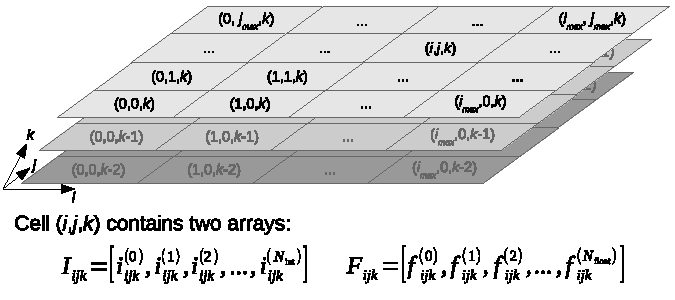
\includegraphics[width=0.8\textwidth]{LatticeModel}}
\end{DoxyImageNoCaption}


Periodic boundary conditions always apply to the first two indices of a cell, but not the third. In a manner similar to that of the software SPPARKS \texorpdfstring{$<$}{<}\href{http://spparks.sandia.gov}{\texttt{ http\+://spparks.\+sandia.\+gov}}\texorpdfstring{$>$}{>}, each cell also contains two one-\/dimensional arrays, one with integer values and one with double precision floating-\/point values. The size of these arrays is the same for all cells. The physical meaning of the contents of the arrays is left up to the client application that uses the ARL \doxylink{namespaceKMCThinFilm}{KMCThin\+Film} library; for a given application, they may be used to identify species of a basis of atoms within a cell, or the spatial coordinates of an atom in a cell in a possibly distorted lattice, or, for a simpler solid-\/on-\/solid application, the height of a column of atoms at $(i,j,0)$. The lattice need not be cubic. If the cells are treated as those of a Bravais lattice with primitive lattice vectors $\mathbf{a}_i$, $\mathbf{a}_j$, and $\mathbf{a}_k$, then the physical location of cell $(i,j,k)$ may be said to be  $\mathbf{a}_i i + \mathbf{a}_j j
+ \mathbf{a}_k k$. The sizes of the arrays in each cell of the lattice, as well as the maximum values of the first two indices of a cell, are fixed when the lattice is initialized, but additional planes may be added to the lattice at any time step of the simulation.\hypertarget{concepts_and_algorithms_kmc_par_alg}{}\doxysection{\texorpdfstring{Parallel approximate Kinetic Monte Carlo algorithm}{Parallel approximate Kinetic Monte Carlo algorithm}}\label{concepts_and_algorithms_kmc_par_alg}
The lattice in a parallel k\+MC simulation is partitioned among the processors in an MPI communicator. There are two methods of decomposition. The simplest is row-\/based decomposition, shown below.

 
\begin{DoxyImageNoCaption}
  \mbox{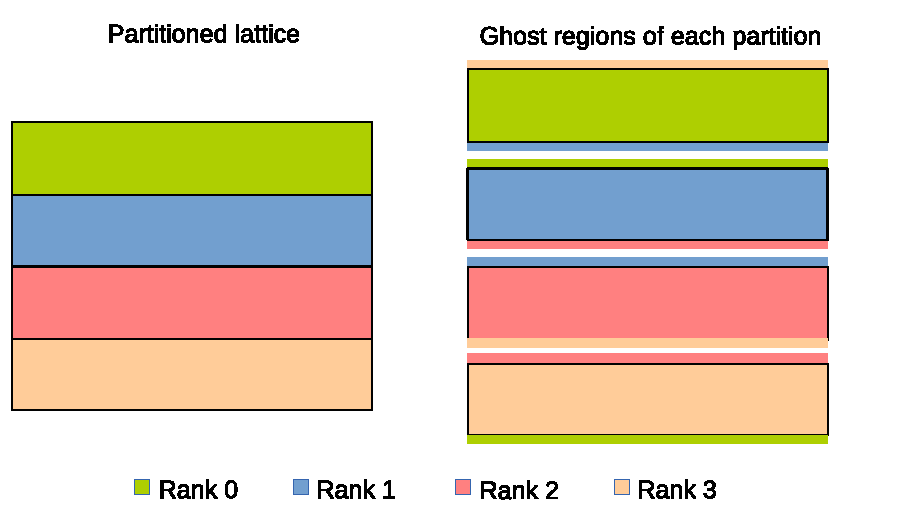
\includegraphics[width=0.7\textwidth]{PartitionedLatticeRow}}
\end{DoxyImageNoCaption}


In the above diagram, a lattice is divided among four processors with ranks ranging from 0 to 3. Here, ``ghost sites'' appear along the top and bottom of each partition of the lattice. The ghost regions along the edges of each partition are copies of the lattice sites of a neighboring processor, and in the diagram, the processor from which they are copied is shown via their color. Periodic boundary conditions are employed here, so that the top of the rank 0 partition is connected to the bottom of the rank 3 partition. Ghost regions are not needed for the left and right sides. Alternatively, the lattice may be decomposed such that the perimeter of each partition is minimized. Here, this is called {\itshape compact} decomposition, and is shown below.

 
\begin{DoxyImageNoCaption}
  \mbox{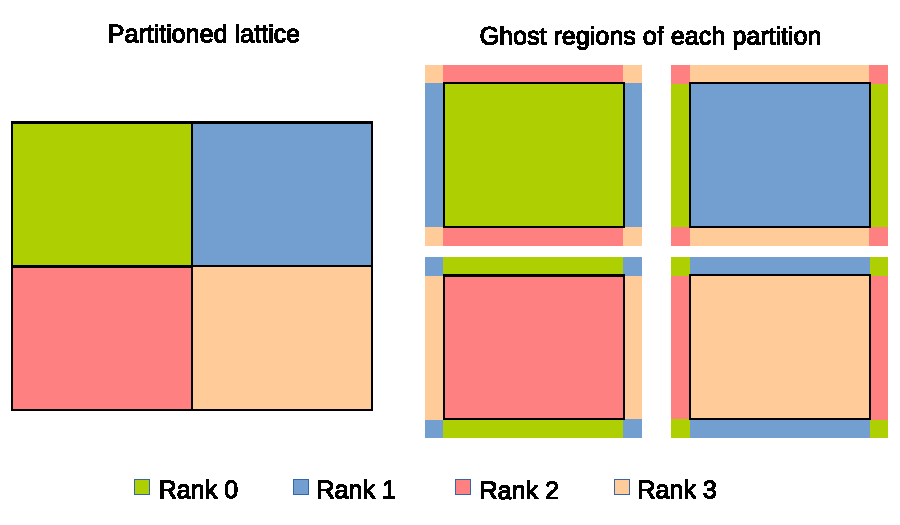
\includegraphics[width=0.8\textwidth]{PartitionedLatticeCompact}}
\end{DoxyImageNoCaption}


Now, ghost regions are along the whole boundary of each portion of the lattice. Again, the lattice is shown divided among four processors with ranks ranging from 0 to 3.

Attempting to do k\+MC simulations on each partition of the lattice would lead to problems at the partition boundaries, since the events done on each partition could lead to conflicting effects on the ghost sites. To avoid this problem, an approximate k\+MC algorithm was developed \cite{shim05}, where each partition is further subdivided into sectors, and at any given time in the simulation, events are executed only for sites within one of these sectors, as illustrated below for the case of compact decomposition.

 
\begin{DoxyImageNoCaption}
  \mbox{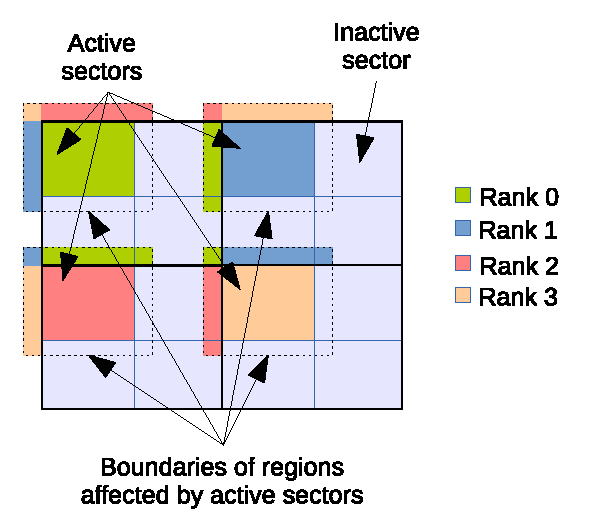
\includegraphics[width=0.5\textwidth]{ActiveSectorsCompact}}
\end{DoxyImageNoCaption}


Partition boundaries are indicated by thick solid lines, while the sector boundaries are indicated by thinner solid lines. Active sectors are shown in the color corresponding to the rank of the partition to which they belong. The dotted lines show the boundaries of the regions affected by events that occur within the active sectors. The parts of these regions that affect ghost sites are shown in the color corresponding to the ranks of the sites of which the ghost sites are copies. If row decomposition were used, there would be two sectors per partition instead of four. Here, in the above diagram, the active sectors happen to be the upper left quadrants of the lattice partitions. At any given time in the simulation, they could be the lower left, lower right, or upper right quadrants, so long as the relative locations of these active sectors are the same for all processors, that is, {\itshape all} upper left, {\itshape all} lower left, and so on. Because the active sectors all have the same relative location, the regions that are affected by events happening within them do not overlap, as illustrated by the diagram above.

With the sectors now defined, the approximate k\+MC algorithm can proceed on each processor as follows\+:


\begin{DoxyEnumerate}
\item Initialize the global time {\itshape t} to zero.
\item Determine the initial value of the stop time $t_{stop}$.
\item Repeat the following until {\itshape t} exceed the desired time $t_{max}$\+:
\begin{DoxyEnumerate}
\item Iterate over the sectors. For each sector visited,
\begin{DoxyEnumerate}
\item initialize the local time $t_{local}$ to zero,
\item update the ghost sites and the set of possible events affected by changes to the ghost sites,
\item run a normal serial k\+MC algorithm on the sites within the sector, incrementing $t_{local}$ as each event is executed until $t_{local} > t_{stop}$, but do not allow the event that would cause $t_{local}$ to exceed $t_{stop}$ to be executed, and
\item update the off-\/processor sites that correspond to the ghost sites that have changed due to the events that have occurred, and again update the set of possible events affected by the ghost site updates.
\end{DoxyEnumerate}
\item Increment the global time {\itshape t} by $t_{stop}$.
\item Update the value of $t_{stop}$.
\end{DoxyEnumerate}
\end{DoxyEnumerate}

The updates of the ghost sites that are performed when a sector is visited do not involve communicating the entirety of the ghost site regions bordering a sector, only the communication of {\itshape changes} to each region.

In principle, the sequence in which the sectors are visited may be random, so long as (1) each processor uses the same random sequences (in order that the active sectors on each processor are at the same relative location, as mentioned previously), and (2) that four sectors are visited before the global time is incremented. However, in the ARL \doxylink{namespaceKMCThinFilm}{KMCThin\+Film} library, the simpler approach seen in another k\+MC code, SPPARKS \cite{plim23}, is taken, where each sector is simply visited in turn in a deterministic loop. In the ARL \doxylink{namespaceKMCThinFilm}{KMCThin\+Film} library, this loop begins at the upper left and then continues to the lower left, followed by the lower right and upper right.

Compact decomposition, despite minimizing the perimeter of each partition, may be slower than row-\/based decomposition, because the former mode of decomposition requires twice as many sectors as the latter, and each visit of a sector requires the communication of ghosts. The volume of data communicated in row-\/based decomposition may indeed be higher than that in compact decomposition. However, since only changes to ghost regions are communicated, this volume is not that high to begin with, so the communication overhead is dominated more by the very acts of sending and receiving messages, rather the costs associated with the size of the data itself. Because of this, row-\/based decomposition is the default in the ARL \doxylink{namespaceKMCThinFilm}{KMCThin\+Film} library.

The value of $t_{stop}$ may be determined by various time-\/stepping schemes. The simplest of these is to set $t_{stop}$ to a fixed value. The other schemes are various kinds of adaptive algorithms, which attempt to determine a reasonable value of $t_{stop}$ from the propensities of the possible events in the simulation. In all of these algorithms, the time step has the general form,   \[t_{stop} = \frac{n_{stop}}{F_{stop}}
\] where $n_{stop}$ is an adjustable parameter, and $F_{stop}$ is a function that determines the particular adaptive time step scheme. Here are the currently available choices for $F_{stop}$\+:


\begin{DoxyItemize}
\item The maximum propensity of all currently possible cell-\/centered events in the simulation. This is a simplified version of the adaptive method of determining $F_{stop}$ recommended by \cite{shim05}. When this method is used, a good conservative value of $n_{stop}$ is 1.\+0, though in some applications, such as island coarsening, a value of up to 10.\+0 has been used without much loss of accuracy \cite{shi07}.
\item The maximum of the average propensities per possible cell-\/centered event from each sector.  $F_{stop} = \max(p_s^1,
  p_s^2, \dots, p_s^{N_{proc}})$, where $N_{proc}$ is the number of processors and for the case of compact decomposition, $p_s^n = \max(p_{s,UL}^n,p_{s,LL}^n,p_{s,LR}^n,p_{s,UR}^n)$, where $p_{s,UL}^n$ is the average propensity of the events in the upper-\/left sector of partition {\itshape n}, that is, the sum of the propensities of all possible events in that sector divided by the number of possible events, and similarly, $p_{s,LL}^n$, $p_{s,LR}^n$, and $p_{s,UR}^n$ are the mean propensities in the lower left, lower right, and upper right sectors of partition {\itshape n}, as in SPPARKS \cite{plim23}. For this choice of $F_{stop}$, a reasonable starting value for $n_{stop}$ is 1.\+0. Note that for a given value of $n_{stop}$, this approach may be less conservative than the previous one.
\end{DoxyItemize}

An additional optional parameter $t_{stop,max}$ may be used with the adaptive schemes. If this parameter is set, then if $n_{stop}/F_{stop} > t_{stop,max}$, $t_{stop}$ will equal $t_{stop,max}$ instead of $n_{stop}/F_{stop}$. This may be useful in cases where the adaptive scheme temporarily overestimates $t_{stop}$ during a simulation.

In a parallel simulation, the propensity of an over-\/lattice event is the propensity per unit area scaled by the in-\/plane area of a {\itshape sector}, rather than the size of a whole monolayer. Also, running a parallel simulation changes how periodic actions are run. In a serial simulation, if a periodic action executes, it executes shortly after an event has been executed. In a parallel simulation, if a periodic action executes, it executes shortly after $t_{stop}$ has been incremented, that is, outside of the looping over sectors. This allows periodic actions to use MPI calls for parallel communication, since a periodic action will execute the same number of times on every processor. 
\chapter{Illustrating the usage of the ARL KMCThin\+Film library by example}
\hypertarget{illustrating_use_by_example}{}\label{illustrating_use_by_example}\index{Illustrating the usage of the ARL KMCThinFilm library by example@{Illustrating the usage of the ARL KMCThinFilm library by example}}
Perhaps the best way to showcase the functionality of the ARL \doxylink{namespaceKMCThinFilm}{KMCThin\+Film} library is to provide examples of its use, so several examples will be shown here. The first example is a very basic solid-\/on-\/solid model and only requires a two-\/dimensional lattice. It is intended to give an overall sense of how the library is meant to be used. The second example shows what is needed to implement a parallel kinetic Monte Carlo simulation with this library. The third example is slightly less simple in that it shows how to implement a three-\/dimensional simulation, and it shows a few other features of the library. The fourth example involves a model of a patterned substrate that encourages two-\/dimensional island formation at regular places along a grid. It is meant to show how the ARL \doxylink{namespaceKMCThinFilm}{KMCThin\+Film} library can be used to speed the implementation of models with features that could require custom code to implement, and again shows some new features of the library not mentioned in previous examples. It is expected that these examples be read {\itshape in order}, since matters discussed in detail in a previous example may be reviewed only briefly, if at all, in later examples. It is also recommended to read all of the examples, in order to get a better overview of the library\textquotesingle{}s features.\hypertarget{illustrating_use_by_example_example_fractal}{}\doxysection{\texorpdfstring{Example\+: Implementation of a ``fractal'' solid-\/on-\/solid model}{Example\+: Implementation of a ``fractal'' solid-\/on-\/solid model}}\label{illustrating_use_by_example_example_fractal}
This example implements a ``fractal'' kinetic Monte Carlo model (similar to that described in the work that developed the approximate semirigorous parallel k\+MC \cite{shim05}). In this simple model, the lattice is simple cubic. The fractal model has two kinds of possible events\+: deposition and diffusion. The deposition flux, i.\+e. propensity per unit area, is {\itshape F} monolayers per unit time. Here, diffusion is a hop of a particle from one lattice site to a nearest neighboring site. Furthermore, in this model, a particle can only diffuse if it has no lateral nearest or next-\/nearest neighbors. This causes the particles to form a surface somewhat reminiscent of snowflakes. If a diffusion event can occur, it occurs with propensity {\itshape D}.

Since this is a solid-\/on-\/solid model, if a diffusing particle moves to a site that is not just above another particle, then the diffusing particle will fall until it lands on top of another particle. This guarantees no vacancies, and it also means that the three-\/dimensional {\itshape true} lattice, where each cell is either occupied or unoccupied, does not have to be explicitly modeled. Instead, a {\itshape computational} lattice is used that has the same lateral dimensions as the cubic true lattice but always contains only a single lattice plane, and the height of the column of particles at cell $(i,j,0)$ of the true lattice is recorded at cell $(i,j,0)$ of the lattice used for computation.

There will actually be {\itshape two} implementations shown in this example\+: one using auto-\/tracking to determine the cells affected by an event, and one using semi-\/manual tracking.\hypertarget{illustrating_use_by_example_ex_fractal_auto_tracking}{}\doxysubsection{\texorpdfstring{Using auto-\/tracking}{Using auto-\/tracking}}\label{illustrating_use_by_example_ex_fractal_auto_tracking}
The code for this example is in the directory {\ttfamily doc/example-\/code/test\+Fractal} of the ARL \doxylink{namespaceKMCThinFilm}{KMCThin\+Film} installation. We will begin by viewing what is effectively the driver file for the simulation code, {\ttfamily test\+Fractal.\+cpp}, which will show the general outline of the simulation, but leave in a few ``blanks'' to be filled in, so to speak. To fill in these blanks, we will then turn to the files {\ttfamily Events\+And\+Actions.\+hpp} and {\ttfamily Events\+And\+Actions.\+cpp}, where the implementation code lies.\hypertarget{illustrating_use_by_example_ex_fractal_driver}{}\doxysubsubsection{\texorpdfstring{Examining the driver code}{Examining the driver code}}\label{illustrating_use_by_example_ex_fractal_driver}
The header files needed by {\ttfamily test\+Fractal.\+cpp} are as follows\+:


\begin{DoxyCodeInclude}{0}
\DoxyCodeLine{\textcolor{preprocessor}{\#include\ <KMCThinFilm/Simulation.hpp>}}
\DoxyCodeLine{\textcolor{preprocessor}{\#include\ <KMCThinFilm/RandNumGenMT19937.hpp>}}
\DoxyCodeLine{}
\DoxyCodeLine{\textcolor{preprocessor}{\#include\ "{}EventsAndActions.hpp"{}}}

\end{DoxyCodeInclude}


The last of these headers, {\ttfamily Events\+And\+Actions.\+hpp}, was mentioned above and will be discussed in more detail later. The remaining headers include the definitions for the \doxylink{classKMCThinFilm_1_1Simulation}{KMCThin\+Film\+::\+Simulation} class and a wrapper class for a Mersenne Twister random number generator. Here, any available concrete implementation of the \doxylink{classKMCThinFilm_1_1RandNumGen}{KMCThin\+Film\+::\+Rand\+Num\+Gen} class could have been used in place of \doxylink{classKMCThinFilm_1_1RandNumGenMT19937}{KMCThin\+Film\+::\+Rand\+Num\+Gen\+MT19937}. In order to avoid having to type the prefix ``{\ttfamily \doxylink{namespaceKMCThinFilm}{KMCThin\+Film}\+:\+:}'' repeatedly, the next line is


\begin{DoxyCodeInclude}{0}
\DoxyCodeLine{\textcolor{keyword}{using\ namespace\ }\mbox{\hyperlink{namespaceKMCThinFilm}{KMCThinFilm}};}

\end{DoxyCodeInclude}


At the beginning of the {\ttfamily main()} function in {\ttfamily test\+Fractal.\+cpp}, we have the following hard-\/coded parameters\+:


\begin{DoxyCodeInclude}{0}
\DoxyCodeLine{\ \ \textcolor{keywordtype}{double}\ F\ =\ 1,\ DoverF\ =\ 1e5,\ maxCoverage\ =\ 4;}
\DoxyCodeLine{\ \ \textcolor{keywordtype}{int}\ domainSize\ =\ 256;}
\DoxyCodeLine{\ \ \textcolor{keywordtype}{unsigned}\ \textcolor{keywordtype}{int}\ seed\ =\ 42;}
\DoxyCodeLine{\ \ \mbox{\hyperlink{namespaceKMCThinFilm_1_1SolverId_a43b0b7ee9ab985e86a13450beb2c7523}{SolverId::Type}}\ sId\ =\ \mbox{\hyperlink{namespaceKMCThinFilm_1_1SolverId_a43b0b7ee9ab985e86a13450beb2c7523a66b6c59bbaeb00525c6dd96af1b33563}{SolverId::DYNAMIC\_SCHULZE}};}

\end{DoxyCodeInclude}


The first several parameters pertain to the fractal model itself. Parameter {\ttfamily F} is the aforementioned deposition flux {\itshape F}, while {\ttfamily DoverF} is {\itshape D}/{\itshape F}. The parameter {\ttfamily max\+Coverage} indicates how many monolayers to deposit, and {\ttfamily domain\+Size} will be used to set the size of the lattice.

The last two parameters relate more to the computation of the kinetic Monte Carlo simulation. The parameter {\ttfamily seed} is the seed for the random number generator. Parameter {\ttfamily s\+Id} indicates which solver will be used to randomly choose an event at a time step in the simulation.

\begin{DoxyNote}{Note}
The parameters are only hard-\/coded in order to simplify the example. In a more realistic simulation code, one could use, for example, the Program Options library of Boost \texorpdfstring{$<$}{<}\href{http://www.boost.org}{\texttt{ http\+://www.\+boost.\+org}}\texorpdfstring{$>$}{>} to input the parameters, especially since Boost is already a dependency of the ARL \doxylink{namespaceKMCThinFilm}{KMCThin\+Film} library.
\end{DoxyNote}
To determine the simulation time needed to deposit the desired number of monolayers, {\ttfamily max\+Coverage} is divided by the flux {\ttfamily F}, so the next line of {\ttfamily test\+Fractal.\+cpp} reads


\begin{DoxyCodeInclude}{0}
\DoxyCodeLine{\ \ \textcolor{keywordtype}{double}\ approxDepTime\ =\ maxCoverage/F;}

\end{DoxyCodeInclude}


At this point, the simulation itself is initialized. To do this, the parameters needed to initialize the lattice used in the simulation are passed to the constructor of a \doxylink{classKMCThinFilm_1_1Simulation}{KMCThin\+Film\+::\+Simulation} object\+:


\begin{DoxyCodeInclude}{0}
\DoxyCodeLine{\ \ \mbox{\hyperlink{structKMCThinFilm_1_1LatticeParams}{LatticeParams}}\ latParams;}
\DoxyCodeLine{\ \ latParams.\mbox{\hyperlink{structKMCThinFilm_1_1LatticeParams_a7a9d46d27758a276fd20d9c18156371a}{numIntsPerCell}}\ =\ FIntVal::SIZE;}
\DoxyCodeLine{\ \ latParams.\mbox{\hyperlink{structKMCThinFilm_1_1LatticeParams_a3a3cc62a6fb5fdda00ed2c63e1ff1020}{globalPlanarDims}}[0]\ =\ latParams.\mbox{\hyperlink{structKMCThinFilm_1_1LatticeParams_a3a3cc62a6fb5fdda00ed2c63e1ff1020}{globalPlanarDims}}[1]\ =\ domainSize;}
\DoxyCodeLine{}
\DoxyCodeLine{\ \ \mbox{\hyperlink{classKMCThinFilm_1_1Simulation}{Simulation}}\ sim(latParams);}

\end{DoxyCodeInclude}


Here, the size of the array of integers in each lattice cell is set to {\ttfamily FInt\+Val\+::\+SIZE}, which will turn out to be an enumeration constant defined in {\ttfamily Events\+And\+Actions.\+hpp}. It was mentioned before that {\ttfamily domain\+Size} will be used to set the size of the lattice. Now here, the lateral size of the lattice has been set to {\ttfamily domain\+Size} {$\times$} {\ttfamily domain\+Size}.

The choice of solver and random number generator for the simulation are now set\+:


\begin{DoxyCodeInclude}{0}
\DoxyCodeLine{\ \ sim.setSolver(sId);}
\DoxyCodeLine{}
\DoxyCodeLine{\ \ \mbox{\hyperlink{namespaceKMCThinFilm_a7b5f253610505f71091c404d12d05aee}{RandNumGenSharedPtr}}\ rng(\textcolor{keyword}{new}\ \mbox{\hyperlink{classKMCThinFilm_1_1RandNumGenMT19937}{RandNumGenMT19937}}(seed));}
\DoxyCodeLine{}
\DoxyCodeLine{\ \ sim.setRNG(rng);}

\end{DoxyCodeInclude}


The order of the above statements matters, since \doxylink{classKMCThinFilm_1_1Simulation_aab6ce6b8f7013c7ce3bcedb8fc3cc469}{KMCThin\+Film\+::\+Simulation\+::set\+RNG()} must be called {\itshape after} \doxylink{classKMCThinFilm_1_1Simulation_adf613f2cf2520695a0fb2ddbbdfd2328}{KMCThin\+Film\+::\+Simulation\+::set\+Solver()}. Here, a ``smart'' pointer to an instance of a \doxylink{classKMCThinFilm_1_1RandNumGen}{KMCThin\+Film\+::\+Rand\+Num\+Gen} class is passed to our \doxylink{classKMCThinFilm_1_1Simulation}{KMCThin\+Film\+::\+Simulation} object, {\ttfamily sim}. Since this is a shared pointer, {\ttfamily sim} does not exclusively own this pointer. Instead, this pointer deletes itself when there are no more references to it. (Also, if need be, other objects besides {\ttfamily sim} are allowed to make use of this pointer to generate random numbers of their own, but that will not be an issue in this simple example.)

At this point, {\itshape possible events} and {\itshape periodic actions} may be added to the simulation. We begin by adding a possible deposition event\+:


\begin{DoxyCodeInclude}{0}
\DoxyCodeLine{\ \ sim.reserveOverLatticeEvents(FOverLatticeEvents::SIZE);}
\DoxyCodeLine{\ \ sim.addOverLatticeEvent(FOverLatticeEvents::DEPOSITION,}
\DoxyCodeLine{\ \ \ \ \ \ \ \ \ \ \ \ \ \ \ \ \ \ \ \ \ \ \ \ \ \ F,\ DepositionExecute);}

\end{DoxyCodeInclude}


This code adds possible so-\/called {\itshape over-\/lattice} events, which are events that may originate from some randomly picked site at the top of the lattice, as discussed in the section entitled ``\doxysectlink{concepts_and_algorithms_kMC_sim_overview}{Basics of kinetic Monte Carlo simulation as implemented in the ARL KMCThin\+Film library}{1}.'' For example, deposition of a particle can be modeled as an event where a particle appears randomly at the top of the lattice and falls until it lands atop an occupied lattice site.

The member function \doxylink{classKMCThinFilm_1_1Simulation_a21587717d5f10a6ae3b8c3606752db13}{KMCThin\+Film\+::\+Simulation\+::reserve\+Over\+Lattice\+Events()} sets the number of possible over-\/lattice events that will be added to the simulation and reserves memory for them. Here, the number of such events is {\ttfamily FOver\+Lattice\+Events\+::\+SIZE}, another enumeration constant defined in {\ttfamily Events\+And\+Actions.\+hpp}. The member function \doxylink{classKMCThinFilm_1_1Simulation_affa3dff53afd248546457944b98376d9}{KMCThin\+Film\+::\+Simulation\+::add\+Over\+Lattice\+Event()} actually adds the event to the simulation. The three arguments that it takes are an integer label identifying the event, which here is another enumeration constant {\ttfamily FOver\+Lattice\+Events\+::\+DEPOSITION}; a propensity per unit of in-\/plane area, that is, the flux {\itshape F}; and a function or function object responsible for actually executing the event, which here is {\ttfamily Deposition\+Execute}. (The actual propensity of the event is the propensity per area scaled by the size of a monolayer of lattice cells, i.\+e., {\ttfamily lat\+Params.\+global\+Planar\+Dims\mbox{[}0\mbox{]}} {$\times$} {\ttfamily lat\+Params.\+global\+Planar\+Dims\mbox{[}1\mbox{]}}.)

We now begin to add {\itshape cell-\/centered} events to the simulation. Again, as discussed in the section entitled ``\doxysectlink{concepts_and_algorithms_kMC_sim_overview}{Basics of kinetic Monte Carlo simulation as implemented in the ARL KMCThin\+Film library}{1},'' these events are called such because such events originate in the neighborhood of some lattice cell, and their propensities---unlike those of over-\/lattice events---{\itshape are} affected by the states of cells in that neighborhood. This neighborhood is defined via one or more {\itshape offsets} from a central cell, as follows\+:


\begin{DoxyCodeInclude}{0}
\DoxyCodeLine{\ \ \mbox{\hyperlink{classKMCThinFilm_1_1CellNeighOffsets}{CellNeighOffsets}}\ hopCNO(HopOffset::SIZE);}
\DoxyCodeLine{}
\DoxyCodeLine{\ \ hopCNO.addOffset(HopOffset::UP,\ \ \ \ \mbox{\hyperlink{classKMCThinFilm_1_1CellIndsOffset}{CellIndsOffset}}(0,+1,0));}
\DoxyCodeLine{\ \ hopCNO.addOffset(HopOffset::DOWN,\ \ \mbox{\hyperlink{classKMCThinFilm_1_1CellIndsOffset}{CellIndsOffset}}(0,-\/1,0));}
\DoxyCodeLine{\ \ hopCNO.addOffset(HopOffset::LEFT,\ \ \mbox{\hyperlink{classKMCThinFilm_1_1CellIndsOffset}{CellIndsOffset}}(-\/1,0,0));}
\DoxyCodeLine{\ \ hopCNO.addOffset(HopOffset::RIGHT,\ \mbox{\hyperlink{classKMCThinFilm_1_1CellIndsOffset}{CellIndsOffset}}(+1,0,0));}
\DoxyCodeLine{}
\DoxyCodeLine{\ \ hopCNO.addOffset(HopOffset::RIGHT\_UP,\ \ \ \mbox{\hyperlink{classKMCThinFilm_1_1CellIndsOffset}{CellIndsOffset}}(+1,+1,0));}
\DoxyCodeLine{\ \ hopCNO.addOffset(HopOffset::RIGHT\_DOWN,\ \mbox{\hyperlink{classKMCThinFilm_1_1CellIndsOffset}{CellIndsOffset}}(+1,-\/1,0));}
\DoxyCodeLine{\ \ hopCNO.addOffset(HopOffset::LEFT\_UP,\ \ \ \ \mbox{\hyperlink{classKMCThinFilm_1_1CellIndsOffset}{CellIndsOffset}}(-\/1,+1,0));}
\DoxyCodeLine{\ \ hopCNO.addOffset(HopOffset::LEFT\_DOWN,\ \ \mbox{\hyperlink{classKMCThinFilm_1_1CellIndsOffset}{CellIndsOffset}}(-\/1,-\/1,0));}

\end{DoxyCodeInclude}


The object {\ttfamily hop\+CNO} is a container of these offsets. In its constructor, it is passed the number of offsets that it will contain, which here is expressed as another enumeration constant, {\ttfamily Hop\+Offset\+::\+SIZE}. The actual offsets are added with the \doxylink{classKMCThinFilm_1_1CellNeighOffsets_a7b983204101cef4973f685d3c68a0106}{KMCThin\+Film\+::\+Cell\+Neigh\+Offsets\+::add\+Offset()}, which takes an integer label greater than zero and less than {\ttfamily Hop\+Offset\+::\+SIZE}, and the offset itself. The integer label 0 (which is also {\ttfamily Hop\+Offset\+::\+SELF}, a constant that will be seen later) is not used as an argument to \doxylink{classKMCThinFilm_1_1CellNeighOffsets_a7b983204101cef4973f685d3c68a0106}{KMCThin\+Film\+::\+Cell\+Neigh\+Offsets\+::add\+Offset()} because it is reserved for the zero offset, i.\+e., {\ttfamily Cell\+Inds\+Offset(0,0,0)}, which is automatically included in a \doxylink{classKMCThinFilm_1_1CellNeighOffsets}{KMCThin\+Film\+::\+Cell\+Neigh\+Offsets} object. The offsets added in the snippet of code above correspond to the positions shown in the figure below\+:

 
\begin{DoxyImageNoCaption}
  \mbox{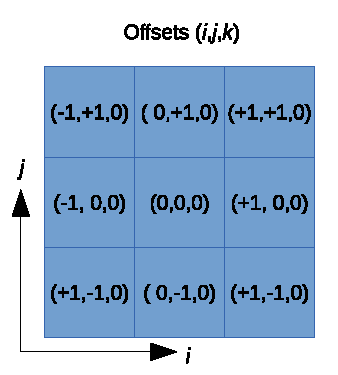
\includegraphics[width=\textwidth,height=\textheight/2,keepaspectratio=true]{OffsetsFractalSim}}
\end{DoxyImageNoCaption}


Since the simulation is on a square lattice, {\itshape i} and {\itshape j} happen to be orthogonal, and the axis along which index {\itshape k} would point is perpendicularly out of the plane. Also, because this is a two-\/dimensional simulation, the third index of the offset, {\itshape k}, is always zero here.

Once the offsets are defined, cell-\/centered events can then be added\+:


\begin{DoxyCodeInclude}{0}
\DoxyCodeLine{\ \ sim.reserveCellCenteredEventGroups(1,FCellCenteredEvents::SIZE);}
\DoxyCodeLine{}
\DoxyCodeLine{\ \ \mbox{\hyperlink{classKMCThinFilm_1_1EventExecutorGroup}{EventExecutorGroup}}\ hopExecs(FCellCenteredEvents::SIZE);}
\DoxyCodeLine{\ \ hopExecs.addEventExecutor(FCellCenteredEvents::HOP\_LEFT,}
\DoxyCodeLine{\ \ \ \ \ \ \ \ \ \ \ \ \ \ \ \ \ \ \ \ \ \ \ \ \ \ \ \ HoppingExecute(FCellCenteredEvents::HOP\_LEFT));}
\DoxyCodeLine{\ \ hopExecs.addEventExecutor(FCellCenteredEvents::HOP\_RIGHT,}
\DoxyCodeLine{\ \ \ \ \ \ \ \ \ \ \ \ \ \ \ \ \ \ \ \ \ \ \ \ \ \ \ \ HoppingExecute(FCellCenteredEvents::HOP\_RIGHT));}
\DoxyCodeLine{\ \ hopExecs.addEventExecutor(FCellCenteredEvents::HOP\_UP,}
\DoxyCodeLine{\ \ \ \ \ \ \ \ \ \ \ \ \ \ \ \ \ \ \ \ \ \ \ \ \ \ \ \ HoppingExecute(FCellCenteredEvents::HOP\_UP));}
\DoxyCodeLine{\ \ hopExecs.addEventExecutor(FCellCenteredEvents::HOP\_DOWN,}
\DoxyCodeLine{\ \ \ \ \ \ \ \ \ \ \ \ \ \ \ \ \ \ \ \ \ \ \ \ \ \ \ \ HoppingExecute(FCellCenteredEvents::HOP\_DOWN));}
\DoxyCodeLine{}
\DoxyCodeLine{\ \ sim.addCellCenteredEventGroup(1,\ hopCNO,}
\DoxyCodeLine{\ \ \ \ \ \ \ \ \ \ \ \ \ \ \ \ \ \ \ \ \ \ \ \ \ \ \ \ \ \ \ \ HoppingPropensity(DoverF*F),}
\DoxyCodeLine{\ \ \ \ \ \ \ \ \ \ \ \ \ \ \ \ \ \ \ \ \ \ \ \ \ \ \ \ \ \ \ \ hopExecs);}

\end{DoxyCodeInclude}


The member function \doxylink{classKMCThinFilm_1_1Simulation_a07827968543d9a9f2cbbdb356b5df8df}{KMCThin\+Film\+::\+Simulation\+::reserve\+Cell\+Centered\+Event\+Groups()} is somewhat analogous to the member function \doxylink{classKMCThinFilm_1_1Simulation_a21587717d5f10a6ae3b8c3606752db13}{KMCThin\+Film\+::\+Simulation\+::reserve\+Over\+Lattice\+Events()} mentioned before. Unlike over-\/lattice events, though, similar types of cell-\/centered events are grouped together. The first argument to this function indicates the number of groups---which is just 1 in this case---while the second argument indicates the total number of individual cell-\/centered event types, regardless of grouping. Here, this number happens to be the enumeration constant {\ttfamily FCell\+Centered\+Events\+::\+SIZE}.

Before actually adding a group of cell-\/centered event types, an \doxylink{classKMCThinFilm_1_1EventExecutorGroup}{KMCThin\+Film\+::\+Event\+Executor\+Group} object must be constructed. This object encapsulates a set of functions or function objects used to execute one of the events in the group of event types, and its constructor takes as an argument the number of function/function objects to be added to the group. Functions and function objects are added to the group in a manner similar to the way offsets are added to a \doxylink{classKMCThinFilm_1_1CellNeighOffsets}{KMCThin\+Film\+::\+Cell\+Neigh\+Offsets} object. Here, the \doxylink{classKMCThinFilm_1_1EventExecutorGroup_a109dab6bc920f3fd6cf7df5d8076a61f}{KMCThin\+Film\+::\+Event\+Executor\+Group\+::add\+Event\+Executor()} takes two arguments\+: an integer label that is greater than or equal to zero and less than {\ttfamily FCell\+Centered\+Events\+::\+SIZE}, and a function/function object satisfying the \doxylink{namespaceKMCThinFilm_a601f0f23e6b591202d40f27df34db951}{KMCThin\+Film\+::\+Event\+Executor\+Auto\+Track} signature.

A group of cell-\/centered event types is added by means of the \doxylink{classKMCThinFilm_1_1Simulation_ada268bce065b942617fd1331b083626d}{KMCThin\+Film\+::\+Simulation\+::add\+Cell\+Centered\+Event\+Group()} member function. This function takes four arguments\+: an integer label identifying the event, which is arbitrarily set to one, a \doxylink{classKMCThinFilm_1_1CellNeighOffsets}{KMCThin\+Film\+::\+Cell\+Neigh\+Offsets} object, which here is {\ttfamily hop\+CNO}, a function or function object used to calculate the propensity of the event, which here is the object {\ttfamily Hopping\+Propensity(\+Dover\+F\texorpdfstring{$\ast$}{*}\+F)}, and the aforementioned \doxylink{classKMCThinFilm_1_1EventExecutorGroup}{KMCThin\+Film\+::\+Event\+Executor\+Group} object. Here, the constructor for the {\ttfamily Hopping\+Propensity} function object class happens to take an argument equal to the hopping propensity {\itshape D}, but that will not necessarily be the case in general.

Finally, we define a time-\/periodic action, which here dumps the state of the lattice to a file at regular intervals of simulation time.


\begin{DoxyCodeInclude}{0}
\DoxyCodeLine{\ \ sim.reserveTimePeriodicActions(PAction::SIZE);}
\DoxyCodeLine{\ \ sim.addTimePeriodicAction(PAction::PRINT,}
\DoxyCodeLine{\ \ \ \ \ \ \ \ \ \ \ \ \ \ \ \ \ \ \ \ \ \ \ \ \ \ \ \ PrintASCII(\textcolor{stringliteral}{"{}snapshot"{}}),}
\DoxyCodeLine{\ \ \ \ \ \ \ \ \ \ \ \ \ \ \ \ \ \ \ \ \ \ \ \ \ \ \ \ 0.05*approxDepTime,\ \textcolor{keyword}{true});}

\end{DoxyCodeInclude}


Again, we have a member function for reserving a type of object, followed by a member function that adds the type of object. The argument to \doxylink{classKMCThinFilm_1_1Simulation_af30c7df97cb00c239325b0500b971a40}{KMCThin\+Film\+::\+Simulation\+::reserve\+Time\+Periodic\+Actions()} is the number of time-\/periodic actions to be added, and as before, this number is represented via an enumeration constant, {\ttfamily PAction\+::\+SIZE}. The member function \doxylink{classKMCThinFilm_1_1Simulation_a2d0b886ef44d3acf0a8c018a7042e1d9}{KMCThin\+Film\+::\+Simulation\+::add\+Time\+Periodic\+Action()} has four arguments\+: an integer label, which here is another enumeration constant {\ttfamily PAction\+::\+PRINT}; a function object to execute the periodic action; the period for the action, which here is taken to be 0.\+05 {$\times$} {\ttfamily approx\+Dep\+Time}; and a Boolean flag to indicate if the action should be performed at the end of a simulation run.

After all this setup, the simulation is then actually set to run as follows\+:


\begin{DoxyCodeInclude}{0}
\DoxyCodeLine{\ \ sim.run(approxDepTime);}
\DoxyCodeLine{\ \ sim.removeOverLatticeEvent(FOverLatticeEvents::DEPOSITION);}
\DoxyCodeLine{\ \ sim.run(0.1*approxDepTime);}

\end{DoxyCodeInclude}


Note that the simulation is run in two stages. In the first stage, there is both diffusion and deposition for a certain amount of time. Then deposition is stopped by removing the deposition event from the simulation. In the second stage, the simulation is run with only diffusion.

(By the way, in this particular fractal model, since particles cannot diffuse if they have any nearest or next nearest neighbors, the simulation soon runs out of particles that can diffuse because the available particles soon acquire neighbors and thus become fixed in place. This causes the simulation to run out of possible events and end before the alloted simulation time is up.)

The general outline of the simulation, as indicated from the driver code, is as follows. First, a simulation object is initialized. Then, possible events and periodic actions are added to the simulation. Finally, the simulation is then run. There are still several ``blanks'' left. Some of these are the enumeration constants. Others are the details of the functions or function objects used to implement the possible events and periodic actions. For these, we turn to an examination of the implementation code in Events\+And\+Actions.\+cpp and its associated header file.\hypertarget{illustrating_use_by_example_ex_fractal_impl}{}\doxysubsubsection{\texorpdfstring{Examining the implementation code}{Examining the implementation code}}\label{illustrating_use_by_example_ex_fractal_impl}
We begin with the header file Events\+And\+Actions.\+hpp. Here we see that the enumerations, rather than being defined directly, are generated from convenience macros defined in \doxylink{MakeEnum_8hpp}{Make\+Enum.\+hpp} from the ARL \doxylink{namespaceKMCThinFilm}{KMCThin\+Film} library. These macros define enumerations associated with adding possible events and actions\+:


\begin{DoxyCodeInclude}{0}
\DoxyCodeLine{\mbox{\hyperlink{MakeEnum_8hpp_a21a6e7611184f517474f1a4628e0e0cb}{KMC\_MAKE\_ID\_ENUM}}(FOverLatticeEvents,}
\DoxyCodeLine{\ \ \ \ \ \ \ \ \ \ \ \ \ \ \ \ \ DEPOSITION);}
\DoxyCodeLine{}
\DoxyCodeLine{\mbox{\hyperlink{MakeEnum_8hpp_a21a6e7611184f517474f1a4628e0e0cb}{KMC\_MAKE\_ID\_ENUM}}(FCellCenteredEvents,}
\DoxyCodeLine{\ \ \ \ \ \ \ \ \ \ \ \ \ \ \ \ \ HOP\_UP,}
\DoxyCodeLine{\ \ \ \ \ \ \ \ \ \ \ \ \ \ \ \ \ HOP\_DOWN,}
\DoxyCodeLine{\ \ \ \ \ \ \ \ \ \ \ \ \ \ \ \ \ HOP\_LEFT,}
\DoxyCodeLine{\ \ \ \ \ \ \ \ \ \ \ \ \ \ \ \ \ HOP\_RIGHT);}
\DoxyCodeLine{}
\DoxyCodeLine{\mbox{\hyperlink{MakeEnum_8hpp_a21a6e7611184f517474f1a4628e0e0cb}{KMC\_MAKE\_ID\_ENUM}}(PAction,}
\DoxyCodeLine{\ \ \ \ \ \ \ \ \ \ \ \ \ \ \ \ \ PRINT);}

\end{DoxyCodeInclude}


The enumerations defined through these macros all include a constant containing the name ``{\ttfamily SIZE}'', which indicates the number of constants in the enumeration (not including {\ttfamily SIZE} itself)\+: {\ttfamily FOver\+Lattice\+Events\+::\+SIZE}, {\ttfamily FCell\+Centered\+Events\+::\+SIZE}, and {\ttfamily PAction\+::\+SIZE}.

The following convenience macro operates similarly\+:


\begin{DoxyCodeInclude}{0}
\DoxyCodeLine{\mbox{\hyperlink{MakeEnum_8hpp_ab74f47ea48cae4ae81e76e45c4fd67c4}{KMC\_MAKE\_LATTICE\_INTVAL\_ENUM}}(F,\ HEIGHT);}

\end{DoxyCodeInclude}


However, the prefix of the enumerations from this macro is not just the first argument of the macro, but the first argument plus ``{\ttfamily Int\+Val}, hence why the constant {\ttfamily FInt\+Val\+::\+SIZE} was seen in the driver code. This macro also defines the constant {\ttfamily FInt\+Val\+::\+HEIGHT}, which will be seen later in the implementation code.

The final macro invocation is


\begin{DoxyCodeInclude}{0}
\DoxyCodeLine{\mbox{\hyperlink{MakeEnum_8hpp_a18b06446141f866d52168964dbc824c7}{KMC\_MAKE\_OFFSET\_ENUM}}(HopOffset,}
\DoxyCodeLine{\ \ \ \ \ \ \ \ \ \ \ \ \ \ \ \ \ \ \ \ \ UP,\ DOWN,\ LEFT,\ RIGHT,}
\DoxyCodeLine{\ \ \ \ \ \ \ \ \ \ \ \ \ \ \ \ \ \ \ \ \ RIGHT\_UP,\ RIGHT\_DOWN,\ LEFT\_UP,\ LEFT\_DOWN);}

\end{DoxyCodeInclude}


This defines the enumeration used to label the offsets between the cell about which an event is centered and the neighboring cells that affect its propensity. Unlike the previously defined enumerations, this one contains {\itshape two} special constants. One of them is {\ttfamily Hop\+Offset\+::\+SIZE}, which as before is the number of constants in the enumeration (not including {\ttfamily SIZE} itself). We have seen this constant used in the driver code as the argument to a constructor of a \doxylink{classKMCThinFilm_1_1CellNeighOffsets}{KMCThin\+Film\+::\+Cell\+Neigh\+Offsets} object. The other is {\ttfamily Hop\+Offset\+::\+SELF}, which identifies {\ttfamily \doxylink{classKMCThinFilm_1_1CellIndsOffset}{Cell\+Inds\+Offset(0,0,0)}}, the offset corresponding to the cell about which an event is centered. This constant will be seen later in the implementation code.

The rest of the lines of the file {\ttfamily Events\+And\+Actions.\+hpp} contain the declarations and definitions for the functions and function objects that define possible events and a periodic action. We now look at these and at their implementations in the file {\ttfamily Events\+And\+Actions.\+cpp}.

Here is the declararation for the function performing deposition\+:


\begin{DoxyCodeInclude}{0}
\DoxyCodeLine{\textcolor{keywordtype}{void}\ DepositionExecute(\textcolor{keyword}{const}\ \mbox{\hyperlink{classKMCThinFilm_1_1CellInds}{KMCThinFilm::CellInds}}\ \&\ ci,}
\DoxyCodeLine{\ \ \ \ \ \ \ \ \ \ \ \ \ \ \ \ \ \ \ \ \ \ \ \textcolor{keyword}{const}\ \mbox{\hyperlink{classKMCThinFilm_1_1SimulationState}{KMCThinFilm::SimulationState}}\ \&\ simState,}
\DoxyCodeLine{\ \ \ \ \ \ \ \ \ \ \ \ \ \ \ \ \ \ \ \ \ \ \ \mbox{\hyperlink{classKMCThinFilm_1_1Lattice}{KMCThinFilm::Lattice}}\ \&\ lattice);}

\end{DoxyCodeInclude}


This function declaration satisfies the \doxylink{namespaceKMCThinFilm_a601f0f23e6b591202d40f27df34db951}{KMCThin\+Film\+::\+Event\+Executor\+Auto\+Track} signature, because it accepts arguments that are references to a \doxylink{classKMCThinFilm_1_1CellInds}{KMCThin\+Film\+::\+Cell\+Inds} object, a \doxylink{classKMCThinFilm_1_1SimulationState}{KMCThin\+Film\+::\+Simulation\+State} object, and a \doxylink{classKMCThinFilm_1_1Lattice}{KMCThin\+Film\+::\+Lattice} object, in that order. Furthermore, since this function is used to alter the lattice, the reference to the \doxylink{classKMCThinFilm_1_1Lattice}{KMCThin\+Film\+::\+Lattice} object is {\itshape not} constant. The implementation of this function is shown below. (It lacks the ``{\ttfamily \doxylink{namespaceKMCThinFilm}{KMCThin\+Film}\+:\+:}'' prefix because {\ttfamily Events\+And\+Actions.\+cpp} begins with the statement ``{\ttfamily using namespace \doxylink{namespaceKMCThinFilm}{KMCThin\+Film};}''.)


\begin{DoxyCodeInclude}{0}
\DoxyCodeLine{\textcolor{keywordtype}{void}\ DepositionExecute(\textcolor{keyword}{const}\ \mbox{\hyperlink{classKMCThinFilm_1_1CellInds}{CellInds}}\ \&\ ci,}
\DoxyCodeLine{\ \ \ \ \ \ \ \ \ \ \ \ \ \ \ \ \ \ \ \ \ \ \ \textcolor{keyword}{const}\ \mbox{\hyperlink{classKMCThinFilm_1_1SimulationState}{SimulationState}}\ \&\ simState,}
\DoxyCodeLine{\ \ \ \ \ \ \ \ \ \ \ \ \ \ \ \ \ \ \ \ \ \ \ \mbox{\hyperlink{classKMCThinFilm_1_1Lattice}{Lattice}}\ \&\ lattice)\ \{}
\DoxyCodeLine{}
\DoxyCodeLine{\ \ \textcolor{keywordtype}{int}\ currVal\ =\ lattice.\mbox{\hyperlink{classKMCThinFilm_1_1Lattice_aff659b471f414c579a51fe280b218ef1}{getInt}}(ci,\ FIntVal::HEIGHT);}
\DoxyCodeLine{\ \ lattice.\mbox{\hyperlink{classKMCThinFilm_1_1Lattice_a81beda29c4c8722cb047f7f2ce0a09ce}{setInt}}(ci,\ FIntVal::HEIGHT,\ currVal\ +\ 1);}
\DoxyCodeLine{}
\DoxyCodeLine{\}}

\end{DoxyCodeInclude}


The argument {\ttfamily ci} represents the \doxylink{classKMCThinFilm_1_1CellInds}{indices of a lattice cell}. Since the function executes an {\itshape over-\/lattice} event, {\ttfamily ci.\+i} and {\ttfamily ci.\+j} are random values, and {\ttfamily ci.\+k} is one less than the current number of lattice planes---which for this two-\/dimensional simulation is simply zero. Essentially what is happening is that the column height at random location $(\mathtt{ci.i}, \mathtt{ci.j}, 0)$ in the lattice is being incremented by one.

In principle, this could have been implemented as class for a function {\itshape object}, that is, a class containing an overload of {\ttfamily operator()}, but here it is an ordinary function for the sake of simplicity. In some later examples, deposition {\itshape is} implemented by a function object class.

\begin{DoxyNote}{Note}
The {\ttfamily sim\+State} argument is not used in this case because the execution of this deposition event does not depend upon time. On the other hand, if, for example, deposition were on a rotating substrate, then it might be possible that deposition could occur along a trajectory whose azimuth was  $2\pi\omega
\times \mathtt{simState.elapsedTime()}$, where $\omega$ is the rate of rotation \cite{cho05}.
\end{DoxyNote}
The function object class {\ttfamily Hopping\+Propensity} is defined as follows\+:


\begin{DoxyCodeInclude}{0}
\DoxyCodeLine{\textcolor{keyword}{class\ }HoppingPropensity\ \{}
\DoxyCodeLine{\textcolor{keyword}{public}:}
\DoxyCodeLine{\ \ HoppingPropensity(\textcolor{keywordtype}{double}\ D)\ :\ D\_(D)\ \{\}}
\DoxyCodeLine{\ \ \textcolor{keywordtype}{void}\ operator()(\textcolor{keyword}{const}\ KMCThinFilm::CellNeighProbe\ \&\ cnp,\ }
\DoxyCodeLine{\ \ \ \ \ \ \ \ \ \ \ \ \ \ \ \ \ \ std::vector<double>\ \&\ propensityVec)\ \textcolor{keyword}{const};}
\DoxyCodeLine{\textcolor{keyword}{private}:}
\DoxyCodeLine{\ \ \textcolor{keywordtype}{double}\ D\_;}
\DoxyCodeLine{\};}

\end{DoxyCodeInclude}


In this class, the private data member {\ttfamily D\+\_\+} stores the hopping propensity {\itshape D}. Also, this class satisfies the \doxylink{namespaceKMCThinFilm_afc58c6c4948aa7d7243beb0990a563f1}{KMCThin\+Film\+::\+Cell\+Centered\+Group\+Propensities} signature, since it contains an overload of {\ttfamily operator()} that takes as arguments a constant reference to a \doxylink{classKMCThinFilm_1_1CellNeighProbe}{KMCThin\+Film\+::\+Cell\+Neigh\+Probe} object and {\itshape non}-\/constant reference to a {\ttfamily std\+::vector} of double precision values. This second argument is an output argument that will be the propensities of hopping in various directions. Before an instance of this function object class even has a chance to execute, the output argument will have already been resized so that it has the same number of elements as there are cell-\/centered events in the group associated with this function object class, and these elements will have been initialized to zero.

Here is the part of the implementation of the function object class that actually calculates the propensity for hopping\+:


\begin{DoxyCodeInclude}{0}
\DoxyCodeLine{\textcolor{keywordtype}{void}\ HoppingPropensity::operator()(\textcolor{keyword}{const}\ \mbox{\hyperlink{classKMCThinFilm_1_1CellNeighProbe}{CellNeighProbe}}\ \&\ cnp,\ }
\DoxyCodeLine{\ \ \ \ \ \ \ \ \ \ \ \ \ \ \ \ \ \ \ \ \ \ \ \ \ \ \ \ \ \ \ \ \ \ \ std::vector<double>\ \&\ propensityVec)\textcolor{keyword}{\ const\ }\{}
\DoxyCodeLine{}
\DoxyCodeLine{\ \ \textcolor{keywordtype}{int}\ currHeight\ =\ cnp.\mbox{\hyperlink{classKMCThinFilm_1_1CellNeighProbe_a7be3ba45264054167a243f15a1954b92}{getInt}}(cnp.\mbox{\hyperlink{classKMCThinFilm_1_1CellNeighProbe_a1ba997186f6326b525dd66df4254d198}{getCellToProbe}}(HopOffset::SELF),\ FIntVal::HEIGHT);}
\DoxyCodeLine{}
\DoxyCodeLine{\ \ \textcolor{keywordflow}{if}\ (currHeight\ >\ 0)\ \{}
\DoxyCodeLine{\ \ \ \ \textcolor{keywordflow}{if}\ ((currHeight\ >\ cnp.\mbox{\hyperlink{classKMCThinFilm_1_1CellNeighProbe_a7be3ba45264054167a243f15a1954b92}{getInt}}(cnp.\mbox{\hyperlink{classKMCThinFilm_1_1CellNeighProbe_a1ba997186f6326b525dd66df4254d198}{getCellToProbe}}(HopOffset::UP),\ FIntVal::HEIGHT))}
\DoxyCodeLine{\ \ \ \ \ \ \ \ \&\&\ (currHeight\ >\ cnp.\mbox{\hyperlink{classKMCThinFilm_1_1CellNeighProbe_a7be3ba45264054167a243f15a1954b92}{getInt}}(cnp.\mbox{\hyperlink{classKMCThinFilm_1_1CellNeighProbe_a1ba997186f6326b525dd66df4254d198}{getCellToProbe}}(HopOffset::DOWN),\ FIntVal::HEIGHT))}
\DoxyCodeLine{\ \ \ \ \ \ \ \ \&\&\ (currHeight\ >\ cnp.\mbox{\hyperlink{classKMCThinFilm_1_1CellNeighProbe_a7be3ba45264054167a243f15a1954b92}{getInt}}(cnp.\mbox{\hyperlink{classKMCThinFilm_1_1CellNeighProbe_a1ba997186f6326b525dd66df4254d198}{getCellToProbe}}(HopOffset::LEFT),\ FIntVal::HEIGHT))}
\DoxyCodeLine{\ \ \ \ \ \ \ \ \&\&\ (currHeight\ >\ cnp.\mbox{\hyperlink{classKMCThinFilm_1_1CellNeighProbe_a7be3ba45264054167a243f15a1954b92}{getInt}}(cnp.\mbox{\hyperlink{classKMCThinFilm_1_1CellNeighProbe_a1ba997186f6326b525dd66df4254d198}{getCellToProbe}}(HopOffset::RIGHT),\ FIntVal::HEIGHT))}
\DoxyCodeLine{\ \ \ \ \ \ \ \ \&\&\ (currHeight\ >\ cnp.\mbox{\hyperlink{classKMCThinFilm_1_1CellNeighProbe_a7be3ba45264054167a243f15a1954b92}{getInt}}(cnp.\mbox{\hyperlink{classKMCThinFilm_1_1CellNeighProbe_a1ba997186f6326b525dd66df4254d198}{getCellToProbe}}(HopOffset::RIGHT\_UP),\ FIntVal::HEIGHT))}
\DoxyCodeLine{\ \ \ \ \ \ \ \ \&\&\ (currHeight\ >\ cnp.\mbox{\hyperlink{classKMCThinFilm_1_1CellNeighProbe_a7be3ba45264054167a243f15a1954b92}{getInt}}(cnp.\mbox{\hyperlink{classKMCThinFilm_1_1CellNeighProbe_a1ba997186f6326b525dd66df4254d198}{getCellToProbe}}(HopOffset::RIGHT\_DOWN),\ FIntVal::HEIGHT))}
\DoxyCodeLine{\ \ \ \ \ \ \ \ \&\&\ (currHeight\ >\ cnp.\mbox{\hyperlink{classKMCThinFilm_1_1CellNeighProbe_a7be3ba45264054167a243f15a1954b92}{getInt}}(cnp.\mbox{\hyperlink{classKMCThinFilm_1_1CellNeighProbe_a1ba997186f6326b525dd66df4254d198}{getCellToProbe}}(HopOffset::LEFT\_UP),\ FIntVal::HEIGHT))}
\DoxyCodeLine{\ \ \ \ \ \ \ \ \&\&\ (currHeight\ >\ cnp.\mbox{\hyperlink{classKMCThinFilm_1_1CellNeighProbe_a7be3ba45264054167a243f15a1954b92}{getInt}}(cnp.\mbox{\hyperlink{classKMCThinFilm_1_1CellNeighProbe_a1ba997186f6326b525dd66df4254d198}{getCellToProbe}}(HopOffset::LEFT\_DOWN),\ FIntVal::HEIGHT)))\ \{}
\DoxyCodeLine{}
\DoxyCodeLine{\ \ \ \ \ \ propensityVec[FCellCenteredEvents::HOP\_LEFT]\ =\ }
\DoxyCodeLine{\ \ \ \ \ \ \ \ propensityVec[FCellCenteredEvents::HOP\_RIGHT]\ =\ }
\DoxyCodeLine{\ \ \ \ \ \ \ \ propensityVec[FCellCenteredEvents::HOP\_UP]\ =\ }
\DoxyCodeLine{\ \ \ \ \ \ \ \ propensityVec[FCellCenteredEvents::HOP\_DOWN]\ =\ D\_;}
\DoxyCodeLine{\ \ \ \ \}}
\DoxyCodeLine{\ \ \}}
\DoxyCodeLine{}
\DoxyCodeLine{\}}

\end{DoxyCodeInclude}


In propensity calculations, access to the lattice is {\itshape indirect} and occurs via the \doxylink{classKMCThinFilm_1_1CellNeighProbe}{KMCThin\+Film\+::\+Cell\+Neigh\+Probe} object. This object can only access cells that can be returned by \doxylink{classKMCThinFilm_1_1CellNeighProbe_a1ba997186f6326b525dd66df4254d198}{KMCThin\+Film\+::\+Cell\+Neigh\+Probe\+::get\+Cell\+To\+Probe}, which takes the integer label of an offset and returns an object that refers to the cell whose indices are the indices of the cell about which the event is centered plus that offset. If the cell indices about which an object is centered are $(i,j,k)$, then {\ttfamily get\+Cell\+To\+Probe(\+Hop\+Offset\+::\+UP)} returns an object referring to the cell with indices $(i,j+1,k)$, {\ttfamily get\+Cell\+To\+Probe(\+Hop\+Offset\+::\+DOWN)} returns an object referring to the cell with indices $(i,j-1,k)$, and so on. Also, {\ttfamily get\+Cell\+To\+Probe(\+Hop\+Offset\+::\+SELF)} returns an object referring to the cell about which the event is centered, that is, $(i,j,k)$.

\begin{DoxyNote}{Note}
The association of offsets with a \doxylink{namespaceKMCThinFilm_afc58c6c4948aa7d7243beb0990a563f1}{KMCThin\+Film\+::\+Cell\+Centered\+Group\+Propensities} object is done in \doxysectlink{illustrating_use_by_example_ex_fractal_driver}{driver code}{3} via calls to \doxylink{classKMCThinFilm_1_1Simulation_ada268bce065b942617fd1331b083626d}{KMCThin\+Film\+::\+Simulation\+::add\+Cell\+Centered\+Event\+Group()}.
\end{DoxyNote}
The reason for using such indirect lattice access is that it forces the implementation of cell-\/centered propensity calculations to use well-\/defined local neighborhoods about the cell where an event is centered, which makes the incremental update of the set of possible events at each time step possible.

The actual propensity calculation itself is simple. The variable {\ttfamily curr\+Height} is the height of the column of particles at cell $(\mathtt{ci.i}, \mathtt{ci.j}, 0)$ in the true lattice. The propensities stored in {\ttfamily propensity\+Vec} are already initially zero, so they only becomes equal to {\ttfamily D\+\_\+} if


\begin{DoxyItemize}
\item the cell  $(\mathtt{ci.i}, \mathtt{ci.j}, \mathtt{currHeight} -
  1)$ in the true lattice is occupied (i.\+e. the column height stored at cell $(\mathtt{ci.i}, \mathtt{ci.j}, 0)$ of the computational lattice is nonzero), and
\item the lateral neighboring sites of cell  $(\mathtt{ci.i},
  \mathtt{ci.j}, \mathtt{currHeight} - 1)$ in the true lattice are empty (i.\+e. the column height stored at cell $(\mathtt{ci.i}, \mathtt{ci.j}, 0)$ in the computational lattice is greater than the column heights stored in the nearest and next-\/nearest neighbors of that cell).
\end{DoxyItemize}

For convenience and ease of reading, the indices used with {\ttfamily propensity\+Vec} are symbolic enumeration constants that correspond to an event type, i.\+e. {\ttfamily propensity\+Vec\mbox{[}FCell\+Centered\+Events\+::\+HOP\+\_\+\+LEFT\mbox{]}} is the propensity for hopping to the left, {\ttfamily propensity\+Vec\mbox{[}FCell\+Centered\+Events\+::\+HOP\+\_\+\+RIGHT\mbox{]}} is the propensity for hopping to the right, and so on.

\begin{DoxyNote}{Note}
Lattice indices start from zero, which is why the indices of the topmost particle of a column would be  $(\mathtt{ci.i},
\mathtt{ci.j}, \mathtt{currHeight} - 1)$, where {\ttfamily curr\+Height} is the height of the column of particles.
\end{DoxyNote}
As a general rule, the propensity of an event centered at a cell should be zero if it cannot happen at that particular cell.

The function object class {\ttfamily Hopping\+Execute} is defined as follows\+:


\begin{DoxyCodeInclude}{0}
\DoxyCodeLine{\textcolor{keyword}{class\ }HoppingExecute\ \{}
\DoxyCodeLine{\textcolor{keyword}{public}:}
\DoxyCodeLine{\ \ HoppingExecute(FCellCenteredEvents::Type\ hopDir);}
\DoxyCodeLine{\ \ \textcolor{keywordtype}{void}\ operator()(\textcolor{keyword}{const}\ KMCThinFilm::CellInds\ \&\ ci,}
\DoxyCodeLine{\ \ \ \ \ \ \ \ \ \ \ \ \ \ \ \ \ \ \textcolor{keyword}{const}\ KMCThinFilm::SimulationState\ \&\ simState,}
\DoxyCodeLine{\ \ \ \ \ \ \ \ \ \ \ \ \ \ \ \ \ \ KMCThinFilm::Lattice\ \&\ lattice)\ \textcolor{keyword}{const};}
\DoxyCodeLine{\textcolor{keyword}{private}:}
\DoxyCodeLine{\ \ \textcolor{keywordtype}{int}\ jump\_i\_,\ jump\_j\_;}
\DoxyCodeLine{\};}

\end{DoxyCodeInclude}


This class satisfies the \doxylink{namespaceKMCThinFilm_a601f0f23e6b591202d40f27df34db951}{KMCThin\+Film\+::\+Event\+Executor\+Auto\+Track} signature, since it contains an overload of {\ttfamily operator()} that accepts arguments that are references to a \doxylink{classKMCThinFilm_1_1CellInds}{KMCThin\+Film\+::\+Cell\+Inds} object, a \doxylink{classKMCThinFilm_1_1SimulationState}{KMCThin\+Film\+::\+Simulation\+State} object, and a \doxylink{classKMCThinFilm_1_1Lattice}{KMCThin\+Film\+::\+Lattice} object, in that order. Again, since this operator is used to alter the lattice, the reference to the \doxylink{classKMCThinFilm_1_1Lattice}{KMCThin\+Film\+::\+Lattice} object is {\itshape not} constant. The constructor for this class is as follows\+:


\begin{DoxyCodeInclude}{0}
\DoxyCodeLine{HoppingExecute::HoppingExecute(FCellCenteredEvents::Type\ hopDir)\ \{}
\DoxyCodeLine{}
\DoxyCodeLine{\ \ \textcolor{keywordflow}{switch}\ (hopDir)\ \{}
\DoxyCodeLine{\ \ \textcolor{keywordflow}{case}\ FCellCenteredEvents::HOP\_UP:}
\DoxyCodeLine{\ \ \ \ jump\_i\_\ =\ 0;}
\DoxyCodeLine{\ \ \ \ jump\_j\_\ =\ 1;}
\DoxyCodeLine{\ \ \ \ \textcolor{keywordflow}{break};}
\DoxyCodeLine{\ \ \textcolor{keywordflow}{case}\ FCellCenteredEvents::HOP\_DOWN:}
\DoxyCodeLine{\ \ \ \ jump\_i\_\ =\ 0;}
\DoxyCodeLine{\ \ \ \ jump\_j\_\ =\ -\/1;}
\DoxyCodeLine{\ \ \ \ \textcolor{keywordflow}{break};}
\DoxyCodeLine{\ \ \textcolor{keywordflow}{case}\ FCellCenteredEvents::HOP\_LEFT:}
\DoxyCodeLine{\ \ \ \ jump\_i\_\ =\ -\/1;}
\DoxyCodeLine{\ \ \ \ jump\_j\_\ =\ 0;}
\DoxyCodeLine{\ \ \ \ \textcolor{keywordflow}{break};}
\DoxyCodeLine{\ \ \textcolor{keywordflow}{case}\ FCellCenteredEvents::HOP\_RIGHT:}
\DoxyCodeLine{\ \ \ \ jump\_i\_\ =\ 1;}
\DoxyCodeLine{\ \ \ \ jump\_j\_\ =\ 0;}
\DoxyCodeLine{\ \ \ \ \textcolor{keywordflow}{break};}
\DoxyCodeLine{\ \ \textcolor{keywordflow}{default}:}
\DoxyCodeLine{\ \ \ \ \mbox{\hyperlink{namespaceKMCThinFilm_a77bd0cec2abe3a269140d80cfea34ed8}{exitWithMsg}}(\textcolor{stringliteral}{"{}Bad\ hop\ direction!"{}});}
\DoxyCodeLine{\ \ \}}
\DoxyCodeLine{\}}

\end{DoxyCodeInclude}


One can see from this constructor that the function object it instantiates can do one of four possible events, namely a hop to one of four nearest neighboring cells.

Here is the part of the implementation of the function object class that actually executes the event\+:


\begin{DoxyCodeInclude}{0}
\DoxyCodeLine{\textcolor{keywordtype}{void}\ HoppingExecute::operator()(\textcolor{keyword}{const}\ \mbox{\hyperlink{classKMCThinFilm_1_1CellInds}{CellInds}}\ \&\ ci,}
\DoxyCodeLine{\ \ \ \ \ \ \ \ \ \ \ \ \ \ \ \ \ \ \ \ \ \ \ \ \ \ \ \ \ \ \ \ \textcolor{keyword}{const}\ \mbox{\hyperlink{classKMCThinFilm_1_1SimulationState}{SimulationState}}\ \&\ simState,}
\DoxyCodeLine{\ \ \ \ \ \ \ \ \ \ \ \ \ \ \ \ \ \ \ \ \ \ \ \ \ \ \ \ \ \ \ \ \mbox{\hyperlink{classKMCThinFilm_1_1Lattice}{Lattice}}\ \&\ lattice)\textcolor{keyword}{\ const\ }\{}
\DoxyCodeLine{}
\DoxyCodeLine{\ \ \mbox{\hyperlink{classKMCThinFilm_1_1CellInds}{CellInds}}\ ciTo(ci.i\ +\ jump\_i\_,\ ci.j\ +\ jump\_j\_,\ ci.k);}
\DoxyCodeLine{}
\DoxyCodeLine{\ \ \textcolor{keywordtype}{int}\ currFrom\ =\ lattice.\mbox{\hyperlink{classKMCThinFilm_1_1Lattice_aff659b471f414c579a51fe280b218ef1}{getInt}}(ci,\ FIntVal::HEIGHT);}
\DoxyCodeLine{\ \ \textcolor{keywordtype}{int}\ currTo\ =\ lattice.\mbox{\hyperlink{classKMCThinFilm_1_1Lattice_aff659b471f414c579a51fe280b218ef1}{getInt}}(ciTo,\ FIntVal::HEIGHT);}
\DoxyCodeLine{\ \ }
\DoxyCodeLine{\ \ lattice.\mbox{\hyperlink{classKMCThinFilm_1_1Lattice_a81beda29c4c8722cb047f7f2ce0a09ce}{setInt}}(ci,\ FIntVal::HEIGHT,\ currFrom\ -\/\ 1);}
\DoxyCodeLine{\ \ lattice.\mbox{\hyperlink{classKMCThinFilm_1_1Lattice_a81beda29c4c8722cb047f7f2ce0a09ce}{setInt}}(ciTo,\ FIntVal::HEIGHT,\ currTo\ +\ 1);}
\DoxyCodeLine{\}}

\end{DoxyCodeInclude}


Here, {\ttfamily ci} is the set of indices of a cell where the cell-\/centered event can happen, rather than just some random location at the top of the lattice as it is for an over-\/lattice event. Since this particular model is two-\/dimensional, {\ttfamily ci.\+k} is always zero. The hopping of a particle from cell $(\mathtt{ci.i}, \mathtt{ci.j}, \mathtt{currFrom} - 1)$ in the true lattice to  $(\mathtt{ciTo.i}, \mathtt{ciTo.j},
\mathtt{currTo})$ is represented in the computational lattice as a decrement of the column height at {\ttfamily ci} and an increment of the column height at {\ttfamily ci\+To}.

Finally, the function object class {\ttfamily Print\+ASCII}, which prints the state of the lattice to a text file, is defined as follows\+:


\begin{DoxyCodeInclude}{0}
\DoxyCodeLine{\textcolor{keyword}{class\ }PrintASCII\ \{}
\DoxyCodeLine{\textcolor{keyword}{public}:}
\DoxyCodeLine{\ \ PrintASCII(\textcolor{keyword}{const}\ std::string\ \&\ fNameRoot)}
\DoxyCodeLine{\ \ \ \ :\ fNameRoot\_(fNameRoot),}
\DoxyCodeLine{\ \ \ \ \ \ snapShotCntr\_(0)}
\DoxyCodeLine{\ \ \{\}}
\DoxyCodeLine{}
\DoxyCodeLine{\ \ \textcolor{keywordtype}{void}\ operator()(\textcolor{keyword}{const}\ KMCThinFilm::SimulationState\ \&\ simState,}
\DoxyCodeLine{\ \ \ \ \ \ \ \ \ \ \ \ \ \ \ \ \ \ KMCThinFilm::Lattice\ \&\ lattice);}
\DoxyCodeLine{}
\DoxyCodeLine{\textcolor{keyword}{private}:}
\DoxyCodeLine{\ \ std::string\ fNameRoot\_;}
\DoxyCodeLine{\ \ \textcolor{keywordtype}{int}\ snapShotCntr\_;}
\DoxyCodeLine{\};}

\end{DoxyCodeInclude}


This code satisfies the function signature \doxylink{namespaceKMCThinFilm_ab48bbcbabdf454a07e2f0edb47404abe}{KMCThin\+Film\+::\+Periodic\+Action}, since it takes as arguments references to a \doxylink{classKMCThinFilm_1_1SimulationState}{KMCThin\+Film\+::\+Simulation\+State} object and a \doxylink{classKMCThinFilm_1_1Lattice}{KMCThin\+Film\+::\+Lattice} object. While this particular periodic action only dumps the state of the lattice, it is possible for a periodic action to change the lattice, which is why the reference to the \doxylink{classKMCThinFilm_1_1Lattice}{KMCThin\+Film\+::\+Lattice} object is {\itshape not} constant.

Here is the implementation of the function object class\+:


\begin{DoxyCodeInclude}{0}
\DoxyCodeLine{\textcolor{keywordtype}{void}\ PrintASCII::operator()(\textcolor{keyword}{const}\ \mbox{\hyperlink{classKMCThinFilm_1_1SimulationState}{SimulationState}}\ \&\ simState,\ \mbox{\hyperlink{classKMCThinFilm_1_1Lattice}{Lattice}}\ \&\ lattice)\ \{}
\DoxyCodeLine{}
\DoxyCodeLine{\ \ ++snapShotCntr\_;}
\DoxyCodeLine{}
\DoxyCodeLine{\ \ std::string\ fName\ =\ fNameRoot\_\ +\ boost::lexical\_cast<std::string>(snapShotCntr\_)\ +\ \textcolor{stringliteral}{"{}.dat"{}};}
\DoxyCodeLine{\ \ \ \ }
\DoxyCodeLine{\ \ std::ofstream\ outFile(fName.c\_str());}
\DoxyCodeLine{}
\DoxyCodeLine{\ \ \mbox{\hyperlink{structKMCThinFilm_1_1LatticePlanarBBox}{LatticePlanarBBox}}\ localPlanarBBox;}
\DoxyCodeLine{\ \ lattice.\mbox{\hyperlink{classKMCThinFilm_1_1Lattice_a1504ff860e046a8965b37dd437a74c52}{getLocalPlanarBBox}}(\textcolor{keyword}{false},\ localPlanarBBox);}
\DoxyCodeLine{}
\DoxyCodeLine{\ \ \textcolor{keywordtype}{int}\ iminGlobal\ =\ localPlanarBBox.\mbox{\hyperlink{structKMCThinFilm_1_1LatticePlanarBBox_a9de43623938e1ceb68c26feafd4cd009}{imin}};}
\DoxyCodeLine{\ \ \textcolor{keywordtype}{int}\ jminGlobal\ =\ localPlanarBBox.\mbox{\hyperlink{structKMCThinFilm_1_1LatticePlanarBBox_aa227140b560487687496bdbaef79d85e}{jmin}};}
\DoxyCodeLine{}
\DoxyCodeLine{\ \ \textcolor{comment}{//\ "{}P1"{}\ here\ is\ short\ for\ "{}Plus\ 1"{}.}}
\DoxyCodeLine{\ \ \textcolor{keywordtype}{int}\ imaxP1Global\ =\ localPlanarBBox.\mbox{\hyperlink{structKMCThinFilm_1_1LatticePlanarBBox_a8bc6629f20496b2845d66f924a04f35a}{imaxP1}};}
\DoxyCodeLine{\ \ \textcolor{keywordtype}{int}\ jmaxP1Global\ =\ localPlanarBBox.\mbox{\hyperlink{structKMCThinFilm_1_1LatticePlanarBBox_abedcda2c34e2bdfe0404e22838ed33dd}{jmaxP1}};}
\DoxyCodeLine{}
\DoxyCodeLine{\ \ outFile\ <<\ \textcolor{stringliteral}{"{}\#\ "{}}\ <<\ iminGlobal\ <<\ \textcolor{stringliteral}{"{}\ "{}}\ <<\ imaxP1Global\ <<\ \textcolor{stringliteral}{"{}\ "{}}\ <<\ jminGlobal\ <<\ \textcolor{stringliteral}{"{}\ "{}}\ <<\ jmaxP1Global}
\DoxyCodeLine{\ \ \ \ \ \ \ \ \ \ <<\ \textcolor{stringliteral}{"{}\ time:"{}}\ <<\ simState.\mbox{\hyperlink{classKMCThinFilm_1_1SimulationState_a01882b6444dedf12543e0a9e7f763f02}{elapsedTime}}()\ <<\ \textcolor{stringliteral}{"{}\(\backslash\)n"{}};}
\DoxyCodeLine{}
\DoxyCodeLine{\ \ \mbox{\hyperlink{classKMCThinFilm_1_1CellInds}{CellInds}}\ ci;\ ci.k\ =\ 0;}
\DoxyCodeLine{\ \ \textcolor{keywordflow}{for}\ (ci.i\ =\ localPlanarBBox.\mbox{\hyperlink{structKMCThinFilm_1_1LatticePlanarBBox_a9de43623938e1ceb68c26feafd4cd009}{imin}};\ ci.i\ <\ localPlanarBBox.\mbox{\hyperlink{structKMCThinFilm_1_1LatticePlanarBBox_a8bc6629f20496b2845d66f924a04f35a}{imaxP1}};\ ++(ci.i))\ \{}
\DoxyCodeLine{\ \ \ \ \textcolor{keywordflow}{for}\ (ci.j\ =\ localPlanarBBox.\mbox{\hyperlink{structKMCThinFilm_1_1LatticePlanarBBox_aa227140b560487687496bdbaef79d85e}{jmin}};\ ci.j\ <\ localPlanarBBox.\mbox{\hyperlink{structKMCThinFilm_1_1LatticePlanarBBox_abedcda2c34e2bdfe0404e22838ed33dd}{jmaxP1}};\ ++(ci.j))\ \{}
\DoxyCodeLine{\ \ \ \ \ \ outFile\ <<\ ci.i\ <<\ \textcolor{stringliteral}{"{}\ "{}}\ <<\ ci.j\ <<\ \textcolor{stringliteral}{"{}\ "{}}}
\DoxyCodeLine{\ \ \ \ \ \ \ \ \ \ \ \ \ \ <<\ lattice.\mbox{\hyperlink{classKMCThinFilm_1_1Lattice_aff659b471f414c579a51fe280b218ef1}{getInt}}(ci,\ FIntVal::HEIGHT)\ <<\ \textcolor{stringliteral}{"{}\(\backslash\)n"{}};}
\DoxyCodeLine{\ \ \ \ \}}
\DoxyCodeLine{\ \ \}}
\DoxyCodeLine{}
\DoxyCodeLine{\ \ outFile.close();}
\DoxyCodeLine{\}}

\end{DoxyCodeInclude}


This code prints a header that indicates the minimum and maximum values of in-\/plane lattice cell indices {\itshape i} and {\itshape j}, and the elapsed time. It then prints the in-\/plane indices of each cell and the column height stored at that cell.

Also, this code is written to in such a way as to facilitate parallelization. Since this is a serial code, \doxylink{classKMCThinFilm_1_1Lattice_ac160d406b29dc80fb72551ad3d74ac3a}{KMCThin\+Film\+::\+Lattice\+::get\+Global\+Planar\+BBox()} could have been used in place of \doxylink{classKMCThinFilm_1_1Lattice_a1504ff860e046a8965b37dd437a74c52}{KMCThin\+Film\+::\+Lattice\+::get\+Local\+Planar\+BBox()} to obtain the minimum and maximum values of the in-\/plane indices. However, the code as written above will also work in parallel to produce a dump to a file of the part of the lattice that a given processor owns, which would {\itshape not} be true if \doxylink{classKMCThinFilm_1_1Lattice_ac160d406b29dc80fb72551ad3d74ac3a}{KMCThin\+Film\+::\+Lattice\+::get\+Global\+Planar\+BBox()} had been used.\hypertarget{illustrating_use_by_example_Results}{}\doxysubsubsection{\texorpdfstring{Results}{Results}}\label{illustrating_use_by_example_Results}
An overhead view of the surface of the ``fractal'' thin film at various simulation times {\itshape t}, from 0.\+20 units to its maximum value of 4.\+0 units, is shown below. Within a given overhead view, black represents the smallest possible height of a column of particles, and white represents the largest.

 
\begin{DoxyImageNoCaption}
  \mbox{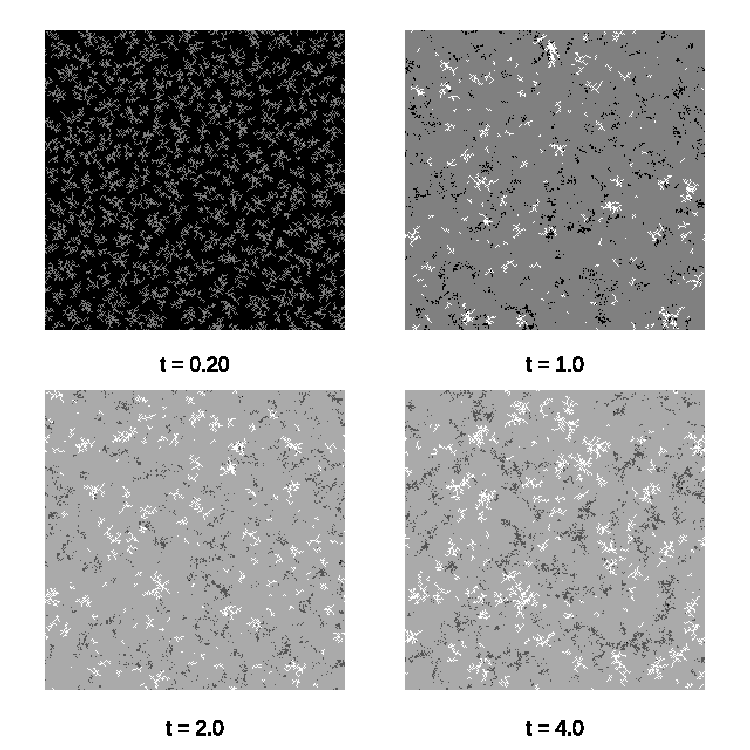
\includegraphics[width=5in]{testFractalSnapshots}}
\end{DoxyImageNoCaption}
\hypertarget{illustrating_use_by_example_ex_fractal_sman_tracking}{}\doxysubsection{\texorpdfstring{Using semi-\/manual tracking}{Using semi-\/manual tracking}}\label{illustrating_use_by_example_ex_fractal_sman_tracking}
The code for this example, which is in the directory {\ttfamily doc/example-\/code/test\+Fractal\+\_\+semi\+\_\+manual\+\_\+track} of the ARL \doxylink{namespaceKMCThinFilm}{KMCThin\+Film} installation, is not much different from that used for previous section ``\doxysectlink{illustrating_use_by_example_ex_fractal_auto_tracking}{Using auto-\/tracking}{2}.''

The source code for the driver file, {\ttfamily test\+Fractal.\+cpp}, mainly differs in how event types are added to the system. The following code is used to add the over-\/lattice event type of deposition to the simulation\+:


\begin{DoxyCodeInclude}{0}
\DoxyCodeLine{\ \ std::vector<CellNeighOffsets>\ tmpExecCNO;}
\DoxyCodeLine{\ \ tmpExecCNO.reserve(1);}
\DoxyCodeLine{}
\DoxyCodeLine{\ \ sim.reserveOverLatticeEvents(FOverLatticeEvents::SIZE);}
\DoxyCodeLine{}
\DoxyCodeLine{\ \ tmpExecCNO.push\_back(\mbox{\hyperlink{classKMCThinFilm_1_1CellNeighOffsets}{CellNeighOffsets}}(1));}
\DoxyCodeLine{\ \ sim.reserveOverLatticeEvents(FOverLatticeEvents::SIZE);}
\DoxyCodeLine{\ \ sim.addOverLatticeEvent(FOverLatticeEvents::DEPOSITION,}
\DoxyCodeLine{\ \ \ \ \ \ \ \ \ \ \ \ \ \ \ \ \ \ \ \ \ \ \ \ \ \ F,\ DepositionExecute,\ tmpExecCNO);}

\end{DoxyCodeInclude}


The member function \doxylink{classKMCThinFilm_1_1Simulation_a21587717d5f10a6ae3b8c3606752db13}{KMCThin\+Film\+::\+Simulation\+::reserve\+Over\+Lattice\+Events()} works the same as before. What differs is the member function \doxylink{classKMCThinFilm_1_1Simulation_affa3dff53afd248546457944b98376d9}{KMCThin\+Film\+::\+Simulation\+::add\+Over\+Lattice\+Event()}, which now has an additional argument, {\ttfamily tmp\+Exec\+CNO}, a {\ttfamily std\+::vector} of \doxylink{classKMCThinFilm_1_1CellNeighOffsets}{KMCThin\+Film\+::\+Cell\+Neigh\+Offsets} objects. For a given deposition event, only one lattice cell is directly changed, so {\ttfamily tmp\+Exec\+CNO} has only one element, which in turn contains only one \doxylink{classKMCThinFilm_1_1CellNeighOffsets}{KMCThin\+Film\+::\+Cell\+Neigh\+Offsets} instance, which contains only the offset that is present in every such instance, $(0,0,0)$. The third argument of \doxylink{classKMCThinFilm_1_1Simulation_affa3dff53afd248546457944b98376d9}{KMCThin\+Film\+::\+Simulation\+::add\+Over\+Lattice\+Event()} is also different, since it satisfies the \doxylink{namespaceKMCThinFilm_a92a9e6c3ced8703f95265e85d80f1797}{KMCThin\+Film\+::\+Event\+Executor\+Semi\+Manual\+Track} signature rather than the \doxylink{namespaceKMCThinFilm_a601f0f23e6b591202d40f27df34db951}{KMCThin\+Film\+::\+Event\+Executor\+Auto\+Track} signature. The following code is used to add a group of cell-\/centered event types\+:


\begin{DoxyCodeInclude}{0}
\DoxyCodeLine{\ \ sim.reserveCellCenteredEventGroups(1,FCellCenteredEvents::SIZE);}
\DoxyCodeLine{}
\DoxyCodeLine{\ \ \mbox{\hyperlink{classKMCThinFilm_1_1EventExecutorGroup}{EventExecutorGroup}}\ hopExecs(FCellCenteredEvents::SIZE);}
\DoxyCodeLine{\ \ tmpExecCNO.clear();}
\DoxyCodeLine{\ \ tmpExecCNO.push\_back(\mbox{\hyperlink{classKMCThinFilm_1_1CellNeighOffsets}{CellNeighOffsets}}(2));}
\DoxyCodeLine{\ \ tmpExecCNO.back().addOffset(1,\ hopCNO.getOffset(HopOffset::LEFT));}
\DoxyCodeLine{}
\DoxyCodeLine{\ \ hopExecs.addEventExecutor(FCellCenteredEvents::HOP\_LEFT,}
\DoxyCodeLine{\ \ \ \ \ \ \ \ \ \ \ \ \ \ \ \ \ \ \ \ \ \ \ \ \ \ \ \ HoppingExecute(),\ tmpExecCNO);}
\DoxyCodeLine{}
\DoxyCodeLine{\ \ tmpExecCNO.back().resetOffsets(2);}
\DoxyCodeLine{\ \ tmpExecCNO.back().addOffset(1,\ hopCNO.getOffset(HopOffset::RIGHT));}
\DoxyCodeLine{\ \ hopExecs.addEventExecutor(FCellCenteredEvents::HOP\_RIGHT,}
\DoxyCodeLine{\ \ \ \ \ \ \ \ \ \ \ \ \ \ \ \ \ \ \ \ \ \ \ \ \ \ \ \ HoppingExecute(),\ tmpExecCNO);}
\DoxyCodeLine{}
\DoxyCodeLine{\ \ tmpExecCNO.back().resetOffsets(2);}
\DoxyCodeLine{\ \ tmpExecCNO.back().addOffset(1,\ hopCNO.getOffset(HopOffset::UP));}
\DoxyCodeLine{\ \ hopExecs.addEventExecutor(FCellCenteredEvents::HOP\_UP,}
\DoxyCodeLine{\ \ \ \ \ \ \ \ \ \ \ \ \ \ \ \ \ \ \ \ \ \ \ \ \ \ \ \ HoppingExecute(),\ tmpExecCNO);}
\DoxyCodeLine{}
\DoxyCodeLine{\ \ tmpExecCNO.back().resetOffsets(2);}
\DoxyCodeLine{\ \ tmpExecCNO.back().addOffset(1,\ hopCNO.getOffset(HopOffset::DOWN));}
\DoxyCodeLine{\ \ hopExecs.addEventExecutor(FCellCenteredEvents::HOP\_DOWN,}
\DoxyCodeLine{\ \ \ \ \ \ \ \ \ \ \ \ \ \ \ \ \ \ \ \ \ \ \ \ \ \ \ \ HoppingExecute(),\ tmpExecCNO);}
\DoxyCodeLine{}
\DoxyCodeLine{\ \ sim.addCellCenteredEventGroup(1,\ hopCNO,}
\DoxyCodeLine{\ \ \ \ \ \ \ \ \ \ \ \ \ \ \ \ \ \ \ \ \ \ \ \ \ \ \ \ \ \ \ \ HoppingPropensity(DoverF*F),}
\DoxyCodeLine{\ \ \ \ \ \ \ \ \ \ \ \ \ \ \ \ \ \ \ \ \ \ \ \ \ \ \ \ \ \ \ \ hopExecs);}

\end{DoxyCodeInclude}


Here, the member functions \doxylink{classKMCThinFilm_1_1Simulation_a07827968543d9a9f2cbbdb356b5df8df}{KMCThin\+Film\+::\+Simulation\+::reserve\+Cell\+Centered\+Event\+Groups()} and \doxylink{classKMCThinFilm_1_1Simulation_ada268bce065b942617fd1331b083626d}{KMCThin\+Film\+::\+Simulation\+::add\+Cell\+Centered\+Event\+Group()} are the same as before. What differs is the way entries are added to the \doxylink{classKMCThinFilm_1_1EventExecutorGroup}{KMCThin\+Film\+::\+Event\+Executor\+Group} instance. Here, \doxylink{classKMCThinFilm_1_1EventExecutorGroup_a109dab6bc920f3fd6cf7df5d8076a61f}{KMCThin\+Film\+::\+Event\+Executor\+Group\+::add\+Event\+Executor()} takes an additional argument, the vector {\ttfamily tmp\+Exec\+CNO}. This vector still contains a single element each time it is used, but since a hopping event changes two lattice cells, this single element contains a \doxylink{classKMCThinFilm_1_1CellNeighOffsets}{KMCThin\+Film\+::\+Cell\+Neigh\+Offsets} instance with two offsets\+: the ever-\/present offset $(0,0,0)$, corresponding to the cell from which a particle hops, and an offset corresponding to the cell to which a particle hops, which depends on the hopping direction. The second argument to \doxylink{classKMCThinFilm_1_1EventExecutorGroup_a109dab6bc920f3fd6cf7df5d8076a61f}{KMCThin\+Film\+::\+Event\+Executor\+Group\+::add\+Event\+Executor()} is also different, since it satisfies the \doxylink{namespaceKMCThinFilm_a92a9e6c3ced8703f95265e85d80f1797}{KMCThin\+Film\+::\+Event\+Executor\+Semi\+Manual\+Track} signature rather than the \doxylink{namespaceKMCThinFilm_a601f0f23e6b591202d40f27df34db951}{KMCThin\+Film\+::\+Event\+Executor\+Auto\+Track} signature.

In {\ttfamily Events\+And\+Actions.\+hpp}, here is the declararation for the function performing deposition\+:


\begin{DoxyCodeInclude}{0}
\DoxyCodeLine{\textcolor{keywordtype}{void}\ DepositionExecute(\textcolor{keyword}{const}\ \mbox{\hyperlink{classKMCThinFilm_1_1CellInds}{KMCThinFilm::CellInds}}\ \&\ ci,}
\DoxyCodeLine{\ \ \ \ \ \ \ \ \ \ \ \ \ \ \ \ \ \ \ \ \ \ \ \textcolor{keyword}{const}\ \mbox{\hyperlink{classKMCThinFilm_1_1SimulationState}{KMCThinFilm::SimulationState}}\ \&\ simState,}
\DoxyCodeLine{\ \ \ \ \ \ \ \ \ \ \ \ \ \ \ \ \ \ \ \ \ \ \ \textcolor{keyword}{const}\ \mbox{\hyperlink{classKMCThinFilm_1_1Lattice}{KMCThinFilm::Lattice}}\ \&\ lattice,}
\DoxyCodeLine{\ \ \ \ \ \ \ \ \ \ \ \ \ \ \ \ \ \ \ \ \ \ \ std::vector<KMCThinFilm::CellsToChange>\ \&\ ctcVec);}

\end{DoxyCodeInclude}


This function declaration satisfies the \doxylink{namespaceKMCThinFilm_a92a9e6c3ced8703f95265e85d80f1797}{KMCThin\+Film\+::\+Event\+Executor\+Semi\+Manual\+Track} signature, because it accepts arguments that are references to a \doxylink{classKMCThinFilm_1_1CellInds}{KMCThin\+Film\+::\+Cell\+Inds} object, a \doxylink{classKMCThinFilm_1_1SimulationState}{KMCThin\+Film\+::\+Simulation\+State} object, a \doxylink{classKMCThinFilm_1_1Lattice}{KMCThin\+Film\+::\+Lattice} object, and a {\ttfamily std\+::vector} of \doxylink{classKMCThinFilm_1_1CellsToChange}{KMCThin\+Film\+::\+Cells\+To\+Change} objects, in that order. Here, the reference to the \doxylink{classKMCThinFilm_1_1Lattice}{KMCThin\+Film\+::\+Lattice} object {\itshape is} constant, since changes to the lattice are forced to occur via \doxylink{classKMCThinFilm_1_1CellsToChange}{KMCThin\+Film\+::\+Cells\+To\+Change} objects. The implementation of this function is shown below.


\begin{DoxyCodeInclude}{0}
\DoxyCodeLine{\textcolor{keywordtype}{void}\ DepositionExecute(\textcolor{keyword}{const}\ \mbox{\hyperlink{classKMCThinFilm_1_1CellInds}{CellInds}}\ \&\ ci,}
\DoxyCodeLine{\ \ \ \ \ \ \ \ \ \ \ \ \ \ \ \ \ \ \ \ \ \ \ \textcolor{keyword}{const}\ \mbox{\hyperlink{classKMCThinFilm_1_1SimulationState}{SimulationState}}\ \&\ simState,}
\DoxyCodeLine{\ \ \ \ \ \ \ \ \ \ \ \ \ \ \ \ \ \ \ \ \ \ \ \textcolor{keyword}{const}\ \mbox{\hyperlink{classKMCThinFilm_1_1Lattice}{KMCThinFilm::Lattice}}\ \&\ lattice,}
\DoxyCodeLine{\ \ \ \ \ \ \ \ \ \ \ \ \ \ \ \ \ \ \ \ \ \ \ std::vector<KMCThinFilm::CellsToChange>\ \&\ ctcVec)\ \{}
\DoxyCodeLine{}
\DoxyCodeLine{\ \ \mbox{\hyperlink{classKMCThinFilm_1_1CellsToChange}{CellsToChange}}\ \&\ ctc\ =\ ctcVec[0];}
\DoxyCodeLine{\ \ ctc.\mbox{\hyperlink{classKMCThinFilm_1_1CellsToChange_a8a56c1106701d5bc3409cd30343fee2c}{setCenter}}(ci);}
\DoxyCodeLine{}
\DoxyCodeLine{\ \ \textcolor{keywordtype}{int}\ currVal\ =\ lattice.\mbox{\hyperlink{classKMCThinFilm_1_1Lattice_aff659b471f414c579a51fe280b218ef1}{getInt}}(ci,\ FIntVal::HEIGHT);}
\DoxyCodeLine{\ \ ctc.\mbox{\hyperlink{classKMCThinFilm_1_1CellsToChange_a62079b840cc200e37e2907ba2e394f78}{setInt}}(0,\ FIntVal::HEIGHT,\ currVal\ +\ 1);}
\DoxyCodeLine{\}}

\end{DoxyCodeInclude}


In general, a \doxylink{classKMCThinFilm_1_1CellsToChange}{KMCThin\+Film\+::\+Cells\+To\+Change} object contains a set of offsets that specifies the relative positions of changed cells, and the \doxylink{classKMCThinFilm_1_1CellsToChange_a8a56c1106701d5bc3409cd30343fee2c}{KMCThin\+Film\+::\+Cells\+To\+Change\+::set\+Center()} member function essentially provides an ``anchor'' used to translate these relative positions to absolute ones. Given a center  $(i_0,
j_0, k_0)$ and offsets $(0,0,0)$, $(o^1_i,o^1_j,o^1_k)$, etc., the absolute coordinates of the cells to change become $(i_0, j_0, k_0)$,  $(i_0 + o^1_i, j_0 + o^1_j, k_0 +
o^1_k)$, etc. Because of how this over-\/lattice event was set up in the driver code, the \doxylink{classKMCThinFilm_1_1CellsToChange}{KMCThin\+Film\+::\+Cells\+To\+Change} object here happens to contain only one offset, $(0,0,0)$, the indices of the cell to be changed are just  $(\mathtt{ci.i}, \mathtt{ci.j},
\mathtt{ci.k})$. The member function \doxylink{classKMCThinFilm_1_1CellsToChange_a62079b840cc200e37e2907ba2e394f78}{KMCThin\+Film\+::\+Cells\+To\+Change\+::set\+Int()} performs the actual change to the cell. This member function is analogous to \doxylink{classKMCThinFilm_1_1Lattice_a81beda29c4c8722cb047f7f2ce0a09ce}{KMCThin\+Film\+::\+Lattice\+::set\+Int()}, except that its first argument is an integer ID corresponding to one of the offsets stored in a \doxylink{classKMCThinFilm_1_1CellsToChange}{KMCThin\+Film\+::\+Cells\+To\+Change} object, rather than a set of cell indices. An integer ID of zero always corresponds to the offset $(0,0,0)$, and accordingly to the indices of the center, which here is $(\mathtt{ci.i}, \mathtt{ci.j}, \mathtt{ci.k})$.

The function object class {\ttfamily Hopping\+Execute} is now defined as follows\+:


\begin{DoxyCodeInclude}{0}
\DoxyCodeLine{\textcolor{keyword}{class\ }HoppingExecute\ \{}
\DoxyCodeLine{\textcolor{keyword}{public}:}
\DoxyCodeLine{\ \ \textcolor{keywordtype}{void}\ operator()(\textcolor{keyword}{const}\ KMCThinFilm::CellInds\ \&\ ci,}
\DoxyCodeLine{\ \ \ \ \ \ \ \ \ \ \ \ \ \ \ \ \ \ \textcolor{keyword}{const}\ KMCThinFilm::SimulationState\ \&\ simState,}
\DoxyCodeLine{\ \ \ \ \ \ \ \ \ \ \ \ \ \ \ \ \ \ \textcolor{keyword}{const}\ KMCThinFilm::Lattice\ \&\ lattice,}
\DoxyCodeLine{\ \ \ \ \ \ \ \ \ \ \ \ \ \ \ \ \ \ std::vector<KMCThinFilm::CellsToChange>\ \&\ ctcVec)\ \textcolor{keyword}{const};}
\DoxyCodeLine{\};}

\end{DoxyCodeInclude}


Since semi-\/manual tracking is used, this class satisfies the \doxylink{namespaceKMCThinFilm_a92a9e6c3ced8703f95265e85d80f1797}{KMCThin\+Film\+::\+Event\+Executor\+Semi\+Manual\+Track} signature, rather than the \doxylink{namespaceKMCThinFilm_a601f0f23e6b591202d40f27df34db951}{KMCThin\+Film\+::\+Event\+Executor\+Auto\+Track} signature. Unlike the previous implementation of the {\ttfamily Hopping\+Execute} class, this one has no private members to indicate the hopping direction, because the hopping direction is determined from the {\ttfamily ctc\+Vec} argument. Here is the part of the implementation of the function object class that actually executes the event\+:


\begin{DoxyCodeInclude}{0}
\DoxyCodeLine{\textcolor{keywordtype}{void}\ HoppingExecute::operator()(\textcolor{keyword}{const}\ \mbox{\hyperlink{classKMCThinFilm_1_1CellInds}{CellInds}}\ \&\ ci,}
\DoxyCodeLine{\ \ \ \ \ \ \ \ \ \ \ \ \ \ \ \ \ \ \ \ \ \ \ \ \ \ \ \ \ \ \ \ \textcolor{keyword}{const}\ \mbox{\hyperlink{classKMCThinFilm_1_1SimulationState}{SimulationState}}\ \&\ simState,}
\DoxyCodeLine{\ \ \ \ \ \ \ \ \ \ \ \ \ \ \ \ \ \ \ \ \ \ \ \ \ \ \ \ \ \ \ \ \textcolor{keyword}{const}\ \mbox{\hyperlink{classKMCThinFilm_1_1Lattice}{KMCThinFilm::Lattice}}\ \&\ lattice,}
\DoxyCodeLine{\ \ \ \ \ \ \ \ \ \ \ \ \ \ \ \ \ \ \ \ \ \ \ \ \ \ \ \ \ \ \ \ std::vector<KMCThinFilm::CellsToChange>\ \&\ ctcVec)\textcolor{keyword}{\ const\ }\{}
\DoxyCodeLine{}
\DoxyCodeLine{\ \ \mbox{\hyperlink{classKMCThinFilm_1_1CellsToChange}{CellsToChange}}\ \&\ ctc\ =\ ctcVec[0];}
\DoxyCodeLine{\ \ ctc.\mbox{\hyperlink{classKMCThinFilm_1_1CellsToChange_a8a56c1106701d5bc3409cd30343fee2c}{setCenter}}(ci);}
\DoxyCodeLine{}
\DoxyCodeLine{\ \ \textcolor{keywordtype}{int}\ currFrom\ =\ lattice.\mbox{\hyperlink{classKMCThinFilm_1_1Lattice_aff659b471f414c579a51fe280b218ef1}{getInt}}(ci,\ FIntVal::HEIGHT);}
\DoxyCodeLine{\ \ \textcolor{keywordtype}{int}\ currTo\ =\ ctc.\mbox{\hyperlink{classKMCThinFilm_1_1CellsToChange_ae559a33ad8206a5e1c8cfd8803ccc765}{getInt}}(1,\ FIntVal::HEIGHT);}
\DoxyCodeLine{\ \ }
\DoxyCodeLine{\ \ ctc.\mbox{\hyperlink{classKMCThinFilm_1_1CellsToChange_a62079b840cc200e37e2907ba2e394f78}{setInt}}(0,\ FIntVal::HEIGHT,\ currFrom\ -\/\ 1);}
\DoxyCodeLine{\ \ ctc.\mbox{\hyperlink{classKMCThinFilm_1_1CellsToChange_a62079b840cc200e37e2907ba2e394f78}{setInt}}(1,\ FIntVal::HEIGHT,\ currTo\ +\ 1);}
\DoxyCodeLine{\}}

\end{DoxyCodeInclude}


Here, {\ttfamily ctc\+Vec} contains a \doxylink{classKMCThinFilm_1_1CellsToChange}{KMCThin\+Film\+::\+Cells\+To\+Change} object with {\itshape two} offsets\+: $(0,0,0)$, which corresponds to the cell from which a particle hops, and an offset that corresponds to the cell to which a particle hops, which depends on the hopping direction. Here we see \doxylink{classKMCThinFilm_1_1CellsToChange_ae559a33ad8206a5e1c8cfd8803ccc765}{KMCThin\+Film\+::\+Cells\+To\+Change\+::get\+Int()} as well as \doxylink{classKMCThinFilm_1_1Lattice_aff659b471f414c579a51fe280b218ef1}{KMCThin\+Film\+::\+Lattice\+::get\+Int()}. The former function is analogous to the latter, with the former function using an integer ID---corresponding to one of the offsets in a \doxylink{classKMCThinFilm_1_1CellsToChange}{KMCThin\+Film\+::\+Cells\+To\+Change} object---instead of cell indices. The integer ID of offset $(0,0,0)$ is, as always,
\begin{DoxyEnumerate}
\item The integer ID of the other offset can be inferred from the portion of the driver code where the offset was set. For example, for rightward hopping, the code to set the offset is
\end{DoxyEnumerate}


\begin{DoxyCodeInclude}{0}
\DoxyCodeLine{\ \ tmpExecCNO.back().resetOffsets(2);}
\DoxyCodeLine{\ \ tmpExecCNO.back().addOffset(1,\ hopCNO.getOffset(HopOffset::RIGHT));}
\DoxyCodeLine{\ \ hopExecs.addEventExecutor(FCellCenteredEvents::HOP\_RIGHT,}
\DoxyCodeLine{\ \ \ \ \ \ \ \ \ \ \ \ \ \ \ \ \ \ \ \ \ \ \ \ \ \ \ \ HoppingExecute(),\ tmpExecCNO);}

\end{DoxyCodeInclude}


The first argument of \doxylink{classKMCThinFilm_1_1CellNeighOffsets_a7b983204101cef4973f685d3c68a0106}{KMCThin\+Film\+::\+Cell\+Neigh\+Offsets\+::add\+Offset()}, which here happens to be 1, is the integer ID for the offset corresponding to the cell to which a particle hops.

The rest of the code of this implementation of a fractal solid-\/on-\/solid model is the same as it is in \doxylink{illustrating_use_by_example_ex_fractal_auto_tracking}{the implementation using auto-\/tracking}.\hypertarget{illustrating_use_by_example_example_fractal_par}{}\doxysection{\texorpdfstring{Example\+: Parallelizing an implementation of a ``fractal'' solid-\/on-\/solid model}{Example\+: Parallelizing an implementation of a ``fractal'' solid-\/on-\/solid model}}\label{illustrating_use_by_example_example_fractal_par}
The code for this example is in the directory {\ttfamily doc/example-\/code/test\+Fractal\+\_\+parallel} of the ARL \doxylink{namespaceKMCThinFilm}{KMCThin\+Film} installation, and it is almost the same as that in {\ttfamily doc/example-\/code/test\+Fractal\+\_\+semi\+\_\+manual\+\_\+track}. Some of the most pertinent differences between the two codes will be discussed here. The parallelized code is actually written so that it can be compiled to either a serial application or an MPI application.

The actual process of parallelizing the code described in the previous section is actually straightforward. Only the driver code, in {\ttfamily test\+Fractal.\+cpp} differs from its serial counterpart, though if the code for dumping the state of the lattice to a file had been different, this might not have been the case. The most obvious changes are near the beginning and the end of the function {\ttfamily main()}, where {\ttfamily MPI\+\_\+\+Init()} and {\ttfamily MPI\+\_\+\+Finalize() are called}\+:


\begin{DoxyCodeInclude}{0}
\DoxyCodeLine{\textcolor{preprocessor}{\#if\ KMC\_PARALLEL}}
\DoxyCodeLine{\ \ MPI\_Init(\&argc,\ \&argv);}
\DoxyCodeLine{\textcolor{preprocessor}{\#endif}}

\end{DoxyCodeInclude}



\begin{DoxyCodeInclude}{0}
\DoxyCodeLine{\textcolor{preprocessor}{\#if\ KMC\_PARALLEL}}
\DoxyCodeLine{\ \ MPI\_Finalize();}
\DoxyCodeLine{\textcolor{preprocessor}{\#endif}}

\end{DoxyCodeInclude}


In order for the driver code to be compilable as serial code, these MPI calls are wrapped by the {\ttfamily \#if KMC\+\_\+\+PARALLEL} and {\ttfamily \#endif} preprocessor directives. Note that {\ttfamily \#if} and {\bfseries{not}} {\ttfamily \#ifdef} is used here.

While most of the parameters near the beginning of {\ttfamily main()} are the same as in the serial version of the code, there is one minor change and one addition, which can be seen below.


\begin{DoxyCodeInclude}{0}
\DoxyCodeLine{\ \ \textcolor{keywordtype}{double}\ F\ =\ 1,\ DoverF\ =\ 1e5,\ maxCoverage\ =\ 4;}
\DoxyCodeLine{\ \ \textcolor{keywordtype}{int}\ domainSize\ =\ 256;}
\DoxyCodeLine{\ \ \textcolor{keywordtype}{unsigned}\ \textcolor{keywordtype}{int}\ seedGlobal\ =\ 42;}
\DoxyCodeLine{\ \ \mbox{\hyperlink{namespaceKMCThinFilm_1_1SolverId_a43b0b7ee9ab985e86a13450beb2c7523}{SolverId::Type}}\ sId\ =\ \mbox{\hyperlink{namespaceKMCThinFilm_1_1SolverId_a43b0b7ee9ab985e86a13450beb2c7523a66b6c59bbaeb00525c6dd96af1b33563}{SolverId::DYNAMIC\_SCHULZE}};}
\DoxyCodeLine{}
\DoxyCodeLine{\ \ \mbox{\hyperlink{classKMCThinFilm_1_1TimeIncr_1_1SchemeVars}{TimeIncr::SchemeVars}}\ schemeVars;}
\DoxyCodeLine{\ \ schemeVars.\mbox{\hyperlink{classKMCThinFilm_1_1TimeIncr_1_1SchemeVars_a9c534dc3967fe996205a22d3b4eb9efc}{setSchemeName}}(\mbox{\hyperlink{namespaceKMCThinFilm_1_1TimeIncr_1_1SchemeName_a9d8be73a26298e6c4379c28285902534ad72ce3a3804cccdfc67fd4debe9cfe9c}{TimeIncr::SchemeName::MAX\_AVG\_PROPENSITY\_PER\_POSS\_EVENT}});}
\DoxyCodeLine{}
\DoxyCodeLine{\ \ schemeVars.\mbox{\hyperlink{classKMCThinFilm_1_1TimeIncr_1_1SchemeVars_a791374d98d976927c656d4adabe19f8d}{setSchemeParam}}(\mbox{\hyperlink{namespaceKMCThinFilm_1_1TimeIncr_1_1SchemeParam_a1ee2f5f6234ea51c6d8ae6993aee48caa1434deeb490996399bdff45a7eb194ee}{TimeIncr::SchemeParam::NSTOP}},\ }
\DoxyCodeLine{\#ifndef\ BAD\_NSTOP}
\DoxyCodeLine{\ \ \ \ \ \ \ \ \ \ \ \ \ \ \ \ \ \ \ \ \ \ \ \ \ \ \ \ 1}
\DoxyCodeLine{\#\textcolor{keywordflow}{else}}
\DoxyCodeLine{\ \ \ \ \ \ \ \ \ \ \ \ \ \ \ \ \ \ \ \ \ \ \ \ \ \ \ \ 100}
\DoxyCodeLine{\#endif}
\DoxyCodeLine{\ \ \ \ \ \ \ \ \ \ \ \ \ \ \ \ \ \ \ \ \ \ \ \ \ \ \ \ );}

\end{DoxyCodeInclude}


The minor change is just a renaming of the variable {\ttfamily seed} to {\ttfamily seed\+Global}, which reflects a change in how the random number generator is initialized in parallel. The addition is the presence of an instance of \doxylink{classKMCThinFilm_1_1TimeIncr_1_1SchemeVars}{KMCThin\+Film\+::\+Time\+Incr\+::\+Scheme\+Vars}, which is used to set the choice of parallel time stepping scheme and any parameter of it. A choice of such a scheme is required to run a parallel Kinetic Monte Carlo simulation. (Parallel time stepping is discussed in the section entitled ``\doxysectlink{concepts_and_algorithms_kmc_par_alg}{Parallel approximate Kinetic Monte Carlo algorithm}{1}.'') The preprocessor variable {\ttfamily BAD\+\_\+\+NSTOP} is used in this example to determine whether the parameter $n_{stop}$ for the parallel time stepping is set to a reasonable value for this simulation, or to one that will produce artifacts.) Unlike the calls to MPI functions, this addition does not have to be placed between {\ttfamily \#if KMC\+\_\+\+PARALLEL} and {\ttfamily \#endif} directives. It simply has no effect in a serial simulation. This is a common practice in the ARL \doxylink{namespaceKMCThinFilm}{KMCThin\+Film} library. Unless a part of its programming interface explicitly involves an MPI data structure, such as {\ttfamily MPI\+\_\+\+Comm}, it will be both legal and harmless in serial code.

Most of the initialization of the simulation, which is shown here,


\begin{DoxyCodeInclude}{0}
\DoxyCodeLine{\ \ \mbox{\hyperlink{structKMCThinFilm_1_1LatticeParams}{LatticeParams}}\ latParams;}
\DoxyCodeLine{\ \ latParams.\mbox{\hyperlink{structKMCThinFilm_1_1LatticeParams_a7a9d46d27758a276fd20d9c18156371a}{numIntsPerCell}}\ =\ FIntVal::SIZE;}
\DoxyCodeLine{\ \ latParams.\mbox{\hyperlink{structKMCThinFilm_1_1LatticeParams_a3a3cc62a6fb5fdda00ed2c63e1ff1020}{globalPlanarDims}}[0]\ =\ latParams.\mbox{\hyperlink{structKMCThinFilm_1_1LatticeParams_a3a3cc62a6fb5fdda00ed2c63e1ff1020}{globalPlanarDims}}[1]\ =\ domainSize;}
\DoxyCodeLine{\ \ latParams.\mbox{\hyperlink{structKMCThinFilm_1_1LatticeParams_addb121738727b46ba00c2c71996f4272}{ghostExtent}}[0]\ =\ latParams.\mbox{\hyperlink{structKMCThinFilm_1_1LatticeParams_addb121738727b46ba00c2c71996f4272}{ghostExtent}}[1]\ =\ 1;}
\DoxyCodeLine{}
\DoxyCodeLine{\textcolor{preprocessor}{\#ifdef\ USE\_COMPACT\_DECOMP}}
\DoxyCodeLine{\ \ latParams.\mbox{\hyperlink{structKMCThinFilm_1_1LatticeParams_a02f5a1a7568e0d94d0127260b4e9dd05}{parallelDecomp}}\ =\ \mbox{\hyperlink{structKMCThinFilm_1_1LatticeParams_ad3f37769b5b30a8f3e941743271def8aa8fc91ae7961264b3e4b8a0706bc01968}{LatticeParams::COMPACT}};}
\DoxyCodeLine{\textcolor{preprocessor}{\#endif}}
\DoxyCodeLine{}
\DoxyCodeLine{\ \ \mbox{\hyperlink{classKMCThinFilm_1_1Simulation}{Simulation}}\ sim(latParams);}

\end{DoxyCodeInclude}


is the same as in the serial simulation, except for a crucial addition\+: specifying the values of the {\ttfamily ghost\+Extent} member of the \doxylink{structKMCThinFilm_1_1LatticeParams}{KMCThin\+Film\+::\+Lattice\+Params} object, which indicate the extent of the ghost region at the edge of each lattice plane. As with the reference to \doxylink{classKMCThinFilm_1_1TimeIncr_1_1SchemeVars}{KMCThin\+Film\+::\+Time\+Incr\+::\+Scheme\+Vars}, there is no need to wrap the statement {\ttfamily lat\+Params.\+ghost\+Extent\mbox{[}0\mbox{]} = lat\+Params.\+ghost\+Extent\mbox{[}1\mbox{]} = 1} within {\ttfamily \#if KMC\+\_\+\+PARALLEL} and {\ttfamily \#endif}, since it simply has no effect in a serial simulation. The preprocessor variable {\ttfamily USE\+\_\+\+COMPACT\+\_\+\+DECOMP} is used in this example to determine whether compact parallel decomposition is used instead of the default row-\/based decomposition. (See the section entitled ``\doxysectlink{concepts_and_algorithms_kmc_par_alg}{Parallel approximate Kinetic Monte Carlo algorithm}{1}"{}"{}'' for a description of methods of decomposition.)

Also, in a parallel simulation, the \doxylink{structKMCThinFilm_1_1LatticeParams}{KMCThin\+Film\+::\+Lattice\+Params} object has an additional member of type {\ttfamily MPI\+\_\+\+Comm}, {\ttfamily lattice\+Comm\+Initial}. By default, this is simply set to {\ttfamily MPI\+\_\+\+COMM\+\_\+\+WORLD}, so there is typically no need to explicitly specify it. However, since it is not defined in the serial version of the ARL \doxylink{namespaceKMCThinFilm}{KMCThin\+Film} library, if there had been any explicit reference to it in the driver code, it would have needed to have been surrounded by {\ttfamily \#if KMC\+\_\+\+PARALLEL} and {\ttfamily \#endif}.

Setting the random number generator becomes slightly more complicated in a parallel simulation, as shown below.


\begin{DoxyCodeInclude}{0}
\DoxyCodeLine{\textcolor{preprocessor}{\#if\ KMC\_PARALLEL}}
\DoxyCodeLine{\ \ \mbox{\hyperlink{namespaceKMCThinFilm_a7b5f253610505f71091c404d12d05aee}{RandNumGenSharedPtr}}\ rng(\textcolor{keyword}{new}\ \mbox{\hyperlink{classKMCThinFilm_1_1RandNumGenDCMT}{RandNumGenDCMT}}(sim.procID(),}
\DoxyCodeLine{\ \ \ \ \ \ \ \ \ \ \ \ \ \ \ \ \ \ \ \ \ \ \ \ \ \ \ \ \ \ \ \ \ \ \ \ \ \ \ \ \ \ \ \ \ seedGlobal,}
\DoxyCodeLine{\ \ \ \ \ \ \ \ \ \ \ \ \ \ \ \ \ \ \ \ \ \ \ \ \ \ \ \ \ \ \ \ \ \ \ \ \ \ \ \ \ \ \ \ \ 123*sim.procID()\ +\ 456,}
\DoxyCodeLine{\ \ \ \ \ \ \ \ \ \ \ \ \ \ \ \ \ \ \ \ \ \ \ \ \ \ \ \ \ \ \ \ \ \ \ \ \ \ \ \ \ \ \ \ \ RandNumGenDCMT::P521));}
\DoxyCodeLine{\textcolor{preprocessor}{\#else}}
\DoxyCodeLine{\ \ \mbox{\hyperlink{namespaceKMCThinFilm_a7b5f253610505f71091c404d12d05aee}{RandNumGenSharedPtr}}\ rng(\textcolor{keyword}{new}\ \mbox{\hyperlink{classKMCThinFilm_1_1RandNumGenMT19937}{RandNumGenMT19937}}(seedGlobal));}
\DoxyCodeLine{\textcolor{preprocessor}{\#endif}}
\DoxyCodeLine{}
\DoxyCodeLine{\ \ sim.setRNG(rng);}

\end{DoxyCodeInclude}


Here, in the serial version of the code, the \doxylink{classKMCThinFilm_1_1RandNumGenMT19937}{KMCThin\+Film\+::\+Rand\+Num\+Gen\+MT19937} is used, while in parallel, \doxylink{classKMCThinFilm_1_1RandNumGenDCMT}{KMCThin\+Film\+::\+Rand\+Num\+Gen\+DCMT} is used. In principle, \doxylink{classKMCThinFilm_1_1RandNumGenDCMT}{KMCThin\+Film\+::\+Rand\+Num\+Gen\+DCMT} could be have been used for both parallel and serial, but \doxylink{classKMCThinFilm_1_1RandNumGenMT19937}{KMCThin\+Film\+::\+Rand\+Num\+Gen\+MT19937} is restricted to serial use. One should also note that the constructor to parallel random number generators such as \doxylink{classKMCThinFilm_1_1RandNumGenDCMT}{KMCThin\+Film\+::\+Rand\+Num\+Gen\+DCMT} takes the MPI rank or processor ID as an argument. Here, this is given by \doxylink{classKMCThinFilm_1_1Simulation_a4007433a9f7d97dd149c2488b7d94e5b}{KMCThin\+Film\+::\+Simulation\+::proc\+ID()}.

Once \doxylink{classKMCThinFilm_1_1Simulation_adf613f2cf2520695a0fb2ddbbdfd2328}{KMCThin\+Film\+::\+Simulation\+::set\+Solver()} has been called, the parallel time step scheme can now be set as follows.


\begin{DoxyCodeInclude}{0}
\DoxyCodeLine{\ \ sim.setTimeIncrScheme(schemeVars);}

\end{DoxyCodeInclude}


Again, there is no need to surround this by {\ttfamily \#if KMC\+\_\+\+PARALLEL} and {\ttfamily \#endif}, since it is just a no-\/op in serial code.

Finally, there is a minor but needed change in the setup for dumping the state of the lattice to files\+:


\begin{DoxyCodeInclude}{0}
\DoxyCodeLine{\ \ sim.reserveTimePeriodicActions(PAction::SIZE);}
\DoxyCodeLine{\ \ sim.addTimePeriodicAction(PAction::PRINT,}
\DoxyCodeLine{\ \ \ \ \ \ \ \ \ \ \ \ \ \ \ \ \ \ \ \ \ \ \ \ \ \ \ \ PrintASCII(\textcolor{stringliteral}{"{}outFile\_ProcCoords"{}}\ +\ }
\DoxyCodeLine{\ \ \ \ \ \ \ \ \ \ \ \ \ \ \ \ \ \ \ \ \ \ \ \ \ \ \ \ \ \ \ \ \ \ \ \ \ \ \ boost::lexical\_cast<std::string>(sim.commCoord(0))\ +\ \textcolor{stringliteral}{"{}\_"{}}\ +}
\DoxyCodeLine{\ \ \ \ \ \ \ \ \ \ \ \ \ \ \ \ \ \ \ \ \ \ \ \ \ \ \ \ \ \ \ \ \ \ \ \ \ \ \ boost::lexical\_cast<std::string>(sim.commCoord(1))\ +\ \textcolor{stringliteral}{"{}\_snapshot"{}}),}
\DoxyCodeLine{\ \ \ \ \ \ \ \ \ \ \ \ \ \ \ \ \ \ \ \ \ \ \ \ \ \ \ \ 0.05*approxDepTime,\ \textcolor{keyword}{true});}

\end{DoxyCodeInclude}


Whereas before in the purely serial code, the root of the names of the dump files was just ``{\ttfamily snapshot}'', now it is a string that is unique to each MPI process. Here, each process writes to its own file, which is not always optimal but will suffice here. In serial code, {\ttfamily sim.\+comm\+Coord(0)} and {\ttfamily sim.\+comm\+Coord(1)} both return an integer value of zero.

When running the parallelized code, two things may be noticed. First, for such a small simulation, it is likely to run {\itshape slower} than the corresponding serial code. Second, whereas the serial code will simply quit when it runs out of possible events to execute, the parallel code will simply continue until the specified simulation time is reached.

The results of the parallel simulations should be about the same as those in the serial simulation, provided that the parameters for the parallel time stepping algorithm are set appropriately. The following results show what may happen if they are not set correctly\+:

 
\begin{DoxyImageNoCaption}
  \mbox{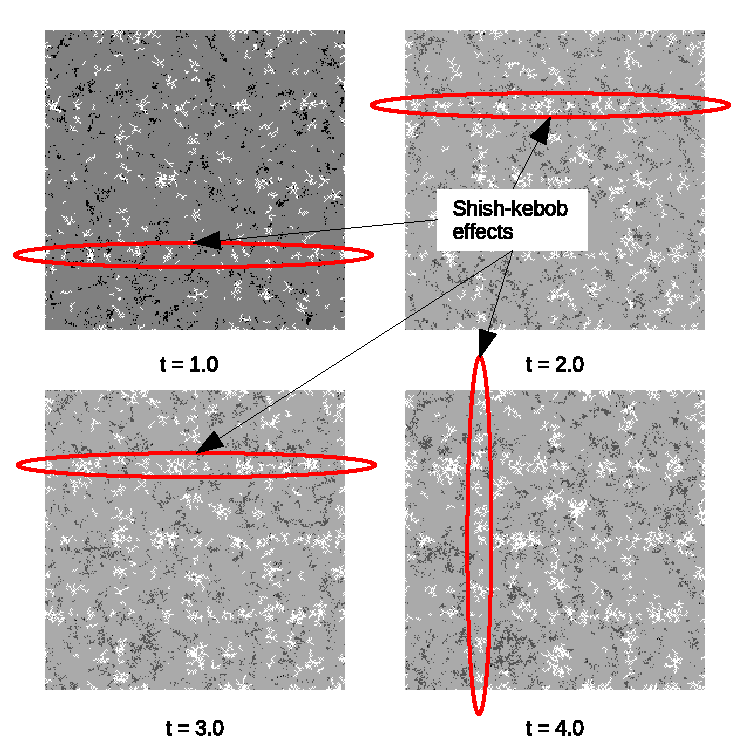
\includegraphics[width=5in]{testParBadSnapshots}}
\end{DoxyImageNoCaption}


These snapshots of the simulated surface, at simulations times {\itshape t} 1.\+0 through 4.\+0, contain artifacts that have been described as a ``shish-\/kebob'' effect \cite{plim23}, where parts of the growing simulated film concentrate on sector boundaries. Some instances of these artifacts have been circled in red. The presence of these artifacts indicates that the size of the parallel time steps is too large.\hypertarget{illustrating_use_by_example_example_baldep}{}\doxysection{\texorpdfstring{Example\+: Implementations of a ballistic deposition model}{Example\+: Implementations of a ballistic deposition model}}\label{illustrating_use_by_example_example_baldep}
While the examples above showcased several features of the ARL \doxylink{namespaceKMCThinFilm}{KMCThin\+Film} library, they were still two-\/dimensional. This particular example is meant to show what is needed for a simulation that requires a three-\/dimensional lattice. It will also show a few other features of the ARL \doxylink{namespaceKMCThinFilm}{KMCThin\+Film} library.

What follows is a pair of example implementations that involve ballistic deposition on a cubic lattice and a contrived cell-\/centered event to change the ``color'' of a lattice cell, which here is a floating-\/point number between zero and one. In ballistic deposition, a depositing particle travels in a straight line until it is close enough to another particle to ``stick'' to it. The result is a deposit that can have several vacancies and overhangs. For simplicity, the depositing particles travel straight downward, which allows the use of simplified algorithms that obviate the need to explicitly model the actual travel of the particle. The propensity of the cell-\/centered event is proportional to the number of occupied nearest neighbors of a lattice cell, including those above and below the cell, and the execution of the event changes the color to an average of the the current cell color and the colors of its occupied nearest neighbors.

In the simplified deposition algorithm \cite{meakin92}, there is both a cubic lattice, whose cells may either be occupied or unoccupied, and an auxiliary two-\/dimensional array of active zone height coordinates, which has the same lateral dimensions as the cubic lattice and may be denoted as $h_a(i,j)$. Before any deposition events begin, the elements of $h_a(i,j)$ are initialized to zero. When a deposition event is chosen, in-\/plane lattice coordinates $(i,j)$ are randomly chosen. Then, a particle is placed at lattice site  $\left(i,j,
h_a(i,j)\right)$, and for each in-\/plane coordinate  $(i_{neigh}, j_{neigh}) \in \{(i+1,j), (i-1,j), (i,j+1),
(i,j-1)\}$, the value of $h_a(i_{neigh}, j_{neigh})$ is checked to see if is less than $h_a(i,j)$. If it is, then it is increased it to the value of $h_a(i,j)$. After this, $h_a(i,j)$ is incremented by one.\hypertarget{illustrating_use_by_example_example_baldep_impl1}{}\doxysubsection{\texorpdfstring{First implementation}{First implementation}}\label{illustrating_use_by_example_example_baldep_impl1}
The code for this implementation is in {\ttfamily doc/example-\/code/test\+Ballistic\+Dep1} of the installation directory of the ARL \doxylink{namespaceKMCThinFilm}{KMCThin\+Film} library. In this implementation, auto-\/tracking has been used. Also, the values of the auxiliary array $h_a(i,j)$ are stored within the first plane of the lattice. Accordingly, in {\ttfamily Events\+And\+Actions.\+hpp}, the following enumeration,


\begin{DoxyCodeInclude}{0}
\DoxyCodeLine{\mbox{\hyperlink{MakeEnum_8hpp_ab74f47ea48cae4ae81e76e45c4fd67c4}{KMC\_MAKE\_LATTICE\_INTVAL\_ENUM}}(BD,\ IS\_OCCUPIED,\ ACTIVE\_ZONE\_HEIGHT);}
\DoxyCodeLine{}
\DoxyCodeLine{\mbox{\hyperlink{MakeEnum_8hpp_aa5359f8f13cbe2c11d54214f49fcf8e8}{KMC\_MAKE\_LATTICE\_FLOATVAL\_ENUM}}(BD,\ COLOR);}

\end{DoxyCodeInclude}


has been defined. The definition for the function object class defining deposition is as follows\+:


\begin{DoxyCodeInclude}{0}
\DoxyCodeLine{\textcolor{keyword}{class\ }DepositionExecute\ \{}
\DoxyCodeLine{\textcolor{keyword}{public}:}
\DoxyCodeLine{\ \ DepositionExecute();}
\DoxyCodeLine{}
\DoxyCodeLine{\ \ \textcolor{keywordtype}{void}\ operator()(\textcolor{keyword}{const}\ KMCThinFilm::CellInds\ \&\ ci,}
\DoxyCodeLine{\ \ \ \ \ \ \ \ \ \ \ \ \ \ \ \ \ \ \textcolor{keyword}{const}\ KMCThinFilm::SimulationState\ \&\ simState,}
\DoxyCodeLine{\ \ \ \ \ \ \ \ \ \ \ \ \ \ \ \ \ \ KMCThinFilm::Lattice\ \&\ lattice);}
\DoxyCodeLine{\textcolor{keyword}{private}:}
\DoxyCodeLine{\ \ std::vector<KMCThinFilm::CellIndsOffset>\ neighOffsets\_;}
\DoxyCodeLine{\};}

\end{DoxyCodeInclude}


The vector {\ttfamily neigh\+Offsets\+\_\+} will be used to find the in-\/plane neighboring lattice cells of the randomly chosen deposition site. This vector is now initialized in the constructor for the deposition function object\+:


\begin{DoxyCodeInclude}{0}
\DoxyCodeLine{DepositionExecute::DepositionExecute()\ \{}
\DoxyCodeLine{\ \ }
\DoxyCodeLine{\ \ neighOffsets\_.reserve(4);}
\DoxyCodeLine{\ \ neighOffsets\_.push\_back(\mbox{\hyperlink{classKMCThinFilm_1_1CellIndsOffset}{CellIndsOffset}}(\ 0,-\/1));}
\DoxyCodeLine{\ \ neighOffsets\_.push\_back(\mbox{\hyperlink{classKMCThinFilm_1_1CellIndsOffset}{CellIndsOffset}}(\ 0,+1));}
\DoxyCodeLine{\ \ neighOffsets\_.push\_back(\mbox{\hyperlink{classKMCThinFilm_1_1CellIndsOffset}{CellIndsOffset}}(-\/1,\ 0));}
\DoxyCodeLine{\ \ neighOffsets\_.push\_back(\mbox{\hyperlink{classKMCThinFilm_1_1CellIndsOffset}{CellIndsOffset}}(+1,\ 0));}
\DoxyCodeLine{}
\DoxyCodeLine{\}}

\end{DoxyCodeInclude}


The implementation of the operator that performs the actual execution of the deposition event is shown below.


\begin{DoxyCodeInclude}{0}
\DoxyCodeLine{\textcolor{keywordtype}{void}\ DepositionExecute::operator()(\textcolor{keyword}{const}\ \mbox{\hyperlink{classKMCThinFilm_1_1CellInds}{CellInds}}\ \&\ ci,}
\DoxyCodeLine{\ \ \ \ \ \ \ \ \ \ \ \ \ \ \ \ \ \ \ \ \ \ \ \ \ \ \ \ \ \ \ \ \ \ \ \textcolor{keyword}{const}\ \mbox{\hyperlink{classKMCThinFilm_1_1SimulationState}{SimulationState}}\ \&\ simState,}
\DoxyCodeLine{\ \ \ \ \ \ \ \ \ \ \ \ \ \ \ \ \ \ \ \ \ \ \ \ \ \ \ \ \ \ \ \ \ \ \ \mbox{\hyperlink{classKMCThinFilm_1_1Lattice}{Lattice}}\ \&\ lattice)\ \{}
\DoxyCodeLine{\ \ }
\DoxyCodeLine{\ \ \textcolor{comment}{/*\ Ballistic\ deposition\ algorithm\ for\ cubic\ lattices\ from\ Meakin\ and}}
\DoxyCodeLine{\textcolor{comment}{\ \ \ \ \ Krug,\ Physical\ Review\ A,\ vol.\ 46,\ num.\ 6,\ pp.\ 3390-\/3399\ (1992).*/}}
\DoxyCodeLine{}
\DoxyCodeLine{\ \ \mbox{\hyperlink{classKMCThinFilm_1_1CellInds}{CellInds}}\ ciInPlane(ci.i,\ ci.j,\ 0);}
\DoxyCodeLine{}
\DoxyCodeLine{\ \ \textcolor{keywordtype}{int}\ kDepAtom\ =\ lattice.\mbox{\hyperlink{classKMCThinFilm_1_1Lattice_aff659b471f414c579a51fe280b218ef1}{getInt}}(ciInPlane,\ BDIntVal::ACTIVE\_ZONE\_HEIGHT);}
\DoxyCodeLine{}
\DoxyCodeLine{\ \ \mbox{\hyperlink{classKMCThinFilm_1_1CellInds}{CellInds}}\ ciTo(ci.i,\ ci.j,\ kDepAtom);}
\DoxyCodeLine{\ \ }
\DoxyCodeLine{\ \ lattice.\mbox{\hyperlink{classKMCThinFilm_1_1Lattice_aa36bda22ed2b0bc8d8737d3d63009765}{addPlanes}}(ciTo.k\ -\/\ ci.k);}
\DoxyCodeLine{\ \ lattice.\mbox{\hyperlink{classKMCThinFilm_1_1Lattice_a81beda29c4c8722cb047f7f2ce0a09ce}{setInt}}(ciTo,\ BDIntVal::IS\_OCCUPIED,\ 1);}
\DoxyCodeLine{}
\DoxyCodeLine{\ \ \textcolor{keywordflow}{for}\ (std::vector<CellIndsOffset>::const\_iterator\ offsetItr\ =\ neighOffsets\_.begin(),}
\DoxyCodeLine{\ \ \ \ \ \ \ \ \ offsetItrEnd\ =\ neighOffsets\_.end();\ offsetItr\ !=\ offsetItrEnd;\ ++offsetItr)\ \{}
\DoxyCodeLine{}
\DoxyCodeLine{\ \ \ \ \mbox{\hyperlink{classKMCThinFilm_1_1CellInds}{CellInds}}\ neighInPlane\ =\ ciInPlane\ +\ *offsetItr;}
\DoxyCodeLine{}
\DoxyCodeLine{\ \ \ \ \textcolor{keywordflow}{if}\ (lattice.\mbox{\hyperlink{classKMCThinFilm_1_1Lattice_aff659b471f414c579a51fe280b218ef1}{getInt}}(neighInPlane,\ BDIntVal::ACTIVE\_ZONE\_HEIGHT)\ <\ kDepAtom)\ \{}
\DoxyCodeLine{\ \ \ \ \ \ lattice.\mbox{\hyperlink{classKMCThinFilm_1_1Lattice_a81beda29c4c8722cb047f7f2ce0a09ce}{setInt}}(neighInPlane,\ BDIntVal::ACTIVE\_ZONE\_HEIGHT,\ kDepAtom);}
\DoxyCodeLine{\ \ \ \ \}}
\DoxyCodeLine{\ \ \}}
\DoxyCodeLine{}
\DoxyCodeLine{\ \ lattice.\mbox{\hyperlink{classKMCThinFilm_1_1Lattice_a81beda29c4c8722cb047f7f2ce0a09ce}{setInt}}(ciInPlane,\ BDIntVal::ACTIVE\_ZONE\_HEIGHT,\ kDepAtom\ +\ 1);}
\DoxyCodeLine{}
\DoxyCodeLine{\}}

\end{DoxyCodeInclude}


Again, the argument {\ttfamily ci} represents the \doxylink{classKMCThinFilm_1_1CellInds}{indices of a lattice cell}. The operator executes an {\itshape over-\/lattice} event, so {\ttfamily ci.\+i} and {\ttfamily ci.\+j} are already random values. This takes care of the part of Meakin\textquotesingle{}s algorithm where a random pair of in-\/plane indices is chosen. The variable {\ttfamily k\+Dep\+Atom} is used to store the current active zone height for the in-\/plane indices  $(\mathtt{ci.i},
\mathtt{ci.j})$. Since the active zone heights are stored only within the {\itshape first} plane of the lattice, {\ttfamily ci\+In\+Plane.\+k} is zero.

Before placing a particle in the lattice cell at {\ttfamily ci\+To}, or  $(\mathtt{ci.i}, \mathtt{ci.j},
\mathtt{kDepAtom})$, it must be ensured that this cell is actually available in the computational lattice. This is what the call to \doxylink{classKMCThinFilm_1_1Lattice_aa36bda22ed2b0bc8d8737d3d63009765}{KMCThin\+Film\+::\+Lattice\+::add\+Planes()} is for. The argument to this member function, if positive, is the number of lattice planes to add. Now {\ttfamily ci.\+k} is initially one less than the maximum number of lattice planes, that is, the maximum possible value of the third lattice coordinate, {\itshape k}. Accordingly, if $\mathtt{ciTo.k} - \mathtt{ci.k}$ is positive, then it is the number of planes that would need to be added to ensure that {\ttfamily ci\+To} is a valid set of indices. If it is zero or negative, then no planes need to be added, and then the call to \doxylink{classKMCThinFilm_1_1Lattice_aa36bda22ed2b0bc8d8737d3d63009765}{KMCThin\+Film\+::\+Lattice\+::add\+Planes()} will simply do nothing. Once the call has been made, \doxylink{classKMCThinFilm_1_1Lattice_a81beda29c4c8722cb047f7f2ce0a09ce}{KMCThin\+Film\+::\+Lattice\+::set\+Int()} can be safely called.

The remainder of the implementation of the operator performing deposition, from the {\ttfamily for} loop onward, simply updates the values of $h_a(i,j)$. The main feature of interest in this remaining part is the \doxylink{namespaceKMCThinFilm_a57489af951d041dc66872aea47fa3da2}{``{\ttfamily +}'' operator} applied to {\ttfamily ci\+In\+Plane} and {\ttfamily \texorpdfstring{$\ast$}{*}offset\+Itr}. The meaning of this operator is such that the statement


\begin{DoxyCode}{0}
\DoxyCodeLine{CellInds\ neighInPlane\ =\ ciInPlane\ +\ *offsetItr;}

\end{DoxyCode}


is equivalent to


\begin{DoxyCode}{0}
\DoxyCodeLine{CellInds\ neighInPlane(ciInPlane.i\ +\ offsetItr-\/>i,}
\DoxyCodeLine{\ \ \ \ \ \ \ \ \ \ \ \ \ \ \ \ \ \ \ \ \ \ ciInPlane.j\ +\ offsetItr-\/>j,}
\DoxyCodeLine{\ \ \ \ \ \ \ \ \ \ \ \ \ \ \ \ \ \ \ \ \ \ ciInPlane.k\ +\ offsetItr-\/>k);}

\end{DoxyCode}


This operator is not commutative; the offset must be its second operand.

Now normally, when \doxylink{classKMCThinFilm_1_1Lattice_aa36bda22ed2b0bc8d8737d3d63009765}{KMCThin\+Film\+::\+Lattice\+::add\+Planes()} is called, the cells that it creates have the quantities associated with them (e.\+g. those labeled as {\ttfamily BDInt\+Val\+::\+IS\+\_\+\+OCCUPIED}, {\ttfamily BDInt\+Val\+::\+ACTIVE\+\_\+\+ZONE\+\_\+\+HEIGHT}, and {\ttfamily BDFloat\+Val\+::\+COLOR}) all set to zero. However, this can be changed, and has been changed for this example. In the initialization of the simulation done via these lines in {\ttfamily test\+Ballistic\+Dep.\+cpp},


\begin{DoxyCodeInclude}{0}
\DoxyCodeLine{\ \ \mbox{\hyperlink{namespaceKMCThinFilm_a7b5f253610505f71091c404d12d05aee}{RandNumGenSharedPtr}}\ rng(\textcolor{keyword}{new}\ \mbox{\hyperlink{classKMCThinFilm_1_1RandNumGenMT19937}{RandNumGenMT19937}}(seed));}
\DoxyCodeLine{}
\DoxyCodeLine{\ \ \mbox{\hyperlink{structKMCThinFilm_1_1LatticeParams}{LatticeParams}}\ latParams;}
\DoxyCodeLine{\ \ latParams.\mbox{\hyperlink{structKMCThinFilm_1_1LatticeParams_a7a9d46d27758a276fd20d9c18156371a}{numIntsPerCell}}\ =\ BDIntVal::SIZE;}
\DoxyCodeLine{\ \ latParams.\mbox{\hyperlink{structKMCThinFilm_1_1LatticeParams_a55263f7f4ef826b814ffeaae27ddf687}{numFloatsPerCell}}\ =\ BDFloatVal::SIZE;}
\DoxyCodeLine{\ \ latParams.\mbox{\hyperlink{structKMCThinFilm_1_1LatticeParams_a3a3cc62a6fb5fdda00ed2c63e1ff1020}{globalPlanarDims}}[0]\ =\ latParams.\mbox{\hyperlink{structKMCThinFilm_1_1LatticeParams_a3a3cc62a6fb5fdda00ed2c63e1ff1020}{globalPlanarDims}}[1]\ =\ domainSize;}
\DoxyCodeLine{\ \ latParams.\mbox{\hyperlink{structKMCThinFilm_1_1LatticeParams_afc58fe3eed9df51a18d9a3fe2ed3b8d1}{setEmptyCellVals}}\ =\ SetEmptyCellWithRandColor(rng);}
\DoxyCodeLine{\ \ latParams.\mbox{\hyperlink{structKMCThinFilm_1_1LatticeParams_a1b5bd22cee6f39342f07f59fb31866c9}{numPlanesToReserve}}\ =\ 100;}
\DoxyCodeLine{}
\DoxyCodeLine{\ \ \mbox{\hyperlink{classKMCThinFilm_1_1Simulation}{Simulation}}\ sim(latParams);}

\end{DoxyCodeInclude}


a special function object, an instance of {\ttfamily Set\+Empty\+Cell\+With\+Rand\+Color}, is used to initialize an empty cell. This function object is defined and implemented in the function files {\ttfamily Init\+Lattice.\+hpp} and {\ttfamily Init\+Lattice.\+cpp}, respectively, which are shown below\+:


\begin{DoxyCodeInclude}{0}
\DoxyCodeLine{\textcolor{preprocessor}{\#ifndef\ INIT\_LATTICE\_HPP}}
\DoxyCodeLine{\textcolor{preprocessor}{\#define\ INIT\_LATTICE\_HPP}}
\DoxyCodeLine{}
\DoxyCodeLine{\textcolor{preprocessor}{\#include\ <KMCThinFilm/Lattice.hpp>}}
\DoxyCodeLine{\textcolor{preprocessor}{\#include\ <KMCThinFilm/RandNumGen.hpp>}}
\DoxyCodeLine{}
\DoxyCodeLine{\textcolor{keyword}{class\ }SetEmptyCellWithRandColor\ \{}
\DoxyCodeLine{\textcolor{keyword}{public}:}
\DoxyCodeLine{\ \ SetEmptyCellWithRandColor(\mbox{\hyperlink{namespaceKMCThinFilm_a7b5f253610505f71091c404d12d05aee}{KMCThinFilm::RandNumGenSharedPtr}}\ rng)}
\DoxyCodeLine{\ \ \ \ :\ rng\_(rng)}
\DoxyCodeLine{\ \ \{\}}
\DoxyCodeLine{}
\DoxyCodeLine{\ \ \textcolor{keywordtype}{void}\ operator()(\textcolor{keyword}{const}\ KMCThinFilm::CellInds\ \&\ ci,}
\DoxyCodeLine{\ \ \ \ \ \ \ \ \ \ \ \ \ \ \ \ \ \ \textcolor{keyword}{const}\ KMCThinFilm::Lattice\ \&\ lattice,}
\DoxyCodeLine{\ \ \ \ \ \ \ \ \ \ \ \ \ \ \ \ \ \ std::vector<int>\ \&\ emptyIntVals,}
\DoxyCodeLine{\ \ \ \ \ \ \ \ \ \ \ \ \ \ \ \ \ \ std::vector<double>\ \&\ emptyFloatVals);}
\DoxyCodeLine{\textcolor{keyword}{private}:}
\DoxyCodeLine{\ \ \mbox{\hyperlink{namespaceKMCThinFilm_a7b5f253610505f71091c404d12d05aee}{KMCThinFilm::RandNumGenSharedPtr}}\ rng\_;}
\DoxyCodeLine{\};}
\DoxyCodeLine{}
\DoxyCodeLine{\textcolor{preprocessor}{\#endif\ }\textcolor{comment}{/*\ INIT\_LATTICE\_HPP\ */}\textcolor{preprocessor}{}}

\end{DoxyCodeInclude}



\begin{DoxyCodeInclude}{0}
\DoxyCodeLine{\textcolor{preprocessor}{\#include\ "{}InitLattice.hpp"{}}}
\DoxyCodeLine{\textcolor{preprocessor}{\#include\ "{}EventsAndActions.hpp"{}}}
\DoxyCodeLine{}
\DoxyCodeLine{\textcolor{keyword}{using\ namespace\ }\mbox{\hyperlink{namespaceKMCThinFilm}{KMCThinFilm}};}
\DoxyCodeLine{}
\DoxyCodeLine{\textcolor{keywordtype}{void}\ SetEmptyCellWithRandColor::operator()(\textcolor{keyword}{const}\ \mbox{\hyperlink{classKMCThinFilm_1_1CellInds}{CellInds}}\ \&\ ci,}
\DoxyCodeLine{\ \ \ \ \ \ \ \ \ \ \ \ \ \ \ \ \ \ \ \ \ \ \ \ \ \ \ \ \ \ \ \ \ \ \ \ \ \ \ \ \ \ \ \textcolor{keyword}{const}\ \mbox{\hyperlink{classKMCThinFilm_1_1Lattice}{Lattice}}\ \&\ lattice,}
\DoxyCodeLine{\ \ \ \ \ \ \ \ \ \ \ \ \ \ \ \ \ \ \ \ \ \ \ \ \ \ \ \ \ \ \ \ \ \ \ \ \ \ \ \ \ \ \ std::vector<int>\ \&\ emptyIntVals,}
\DoxyCodeLine{\ \ \ \ \ \ \ \ \ \ \ \ \ \ \ \ \ \ \ \ \ \ \ \ \ \ \ \ \ \ \ \ \ \ \ \ \ \ \ \ \ \ \ std::vector<double>\ \&\ emptyFloatVals)\ \{}
\DoxyCodeLine{\ \ }
\DoxyCodeLine{\ \ emptyFloatVals[BDFloatVal::COLOR]\ =\ rng\_-\/>getNumInOpenIntervalFrom0To1();}
\DoxyCodeLine{\ \ }
\DoxyCodeLine{\}}

\end{DoxyCodeInclude}


Here, even an ``empty'' lattice cell has a color associated with it, which is randomly determined. Note that there is no need to resize the vectors used as output arguments of {\ttfamily Set\+Empty\+Cell\+With\+Rand\+Color\+::operator()}, since the sizes of these vectors have already been set to the number of integer and floating-\/point quantities, respectively, at each lattice cell.

Since multiple lattice planes will be added during the course of the simulation, {\ttfamily lat\+Params.\+num\+Planes\+To\+Reserve} is set to roughly the number of planes that might be added. This reserves space in memory for those planes but does not add them to the lattice outright. Actually adding the planes is done by \doxylink{classKMCThinFilm_1_1Lattice_aa36bda22ed2b0bc8d8737d3d63009765}{KMCThin\+Film\+::\+Lattice\+::add\+Planes()}. {\ttfamily lat\+Params.\+num\+Planes\+To\+Reserve} is {\itshape not} a hard limit on the number of lattice planes that may be added; it merely affects performance.

\begin{DoxyNote}{Note}
While this example of a means of initializing an empty lattice is contrived, a not-\/so contrived example would be a case where the lattice is distorted and the current coordinates of a particle, which may be near rather than exactly at a lattice site, are stored at a lattice cell. In a new empty cell, it would make sense for these coordinates to be initialized not to zero, but rather to some function of the lattice indices $(i,j,k)$, e.\+g.  $\mathbf{a}_i i + \mathbf{a}_j j + \mathbf{a}_k k +
\mathbf{b}$, where $\mathbf{a}_i$, $\mathbf{a}_j$, and $\mathbf{a}_k$ are primitive lattice vectors and $\mathbf{b}$ is a basis vector.
\end{DoxyNote}
The enumeration associated with the offsets used in the function object classes involved in the color change in a lattice cell is as follows\+:


\begin{DoxyCodeInclude}{0}
\DoxyCodeLine{\mbox{\hyperlink{MakeEnum_8hpp_a18b06446141f866d52168964dbc824c7}{KMC\_MAKE\_OFFSET\_ENUM}}(MIX\_OFFSET,}
\DoxyCodeLine{\ \ \ \ \ \ \ \ \ \ \ \ \ \ \ \ \ \ \ \ \ NORTH,\ SOUTH,\ WEST,\ EAST\ \textcolor{comment}{/*\ First\ four\ neighbors\ are\ lateral\ */},\ }
\DoxyCodeLine{\ \ \ \ \ \ \ \ \ \ \ \ \ \ \ \ \ \ \ \ \ UP,\ DOWN);}

\end{DoxyCodeInclude}


The definition for the function object class defining the propensity for the color change in a lattice cell is


\begin{DoxyCodeInclude}{0}
\DoxyCodeLine{\textcolor{keyword}{class\ }ColorMixPropensity\ \{}
\DoxyCodeLine{\textcolor{keyword}{public}:}
\DoxyCodeLine{\ \ ColorMixPropensity(\textcolor{keywordtype}{double}\ mixPropPerNeighbor)}
\DoxyCodeLine{\ \ \ \ :\ mixPropPerNeighbor\_(mixPropPerNeighbor)}
\DoxyCodeLine{\ \ \{\}\ }
\DoxyCodeLine{}
\DoxyCodeLine{\ \ \textcolor{keywordtype}{void}\ operator()(\textcolor{keyword}{const}\ KMCThinFilm::CellNeighProbe\ \&\ cnp,}
\DoxyCodeLine{\ \ \ \ \ \ \ \ \ \ \ \ \ \ \ \ \ \ std::vector<double>\ \&\ propensityVec)\ \textcolor{keyword}{const};}
\DoxyCodeLine{\textcolor{keyword}{private}:}
\DoxyCodeLine{\ \ \textcolor{keywordtype}{double}\ mixPropPerNeighbor\_;}
\DoxyCodeLine{\};}

\end{DoxyCodeInclude}


and its implementation is


\begin{DoxyCodeInclude}{0}
\DoxyCodeLine{\textcolor{keywordtype}{void}\ ColorMixPropensity::operator()(\textcolor{keyword}{const}\ \mbox{\hyperlink{classKMCThinFilm_1_1CellNeighProbe}{KMCThinFilm::CellNeighProbe}}\ \&\ cnp,}
\DoxyCodeLine{\ \ \ \ \ \ \ \ \ \ \ \ \ \ \ \ \ \ \ \ \ \ \ \ \ \ \ \ \ \ \ \ \ \ \ \ std::vector<double>\ \&\ propensityVec)\textcolor{keyword}{\ const\ }\{}
\DoxyCodeLine{\ \ }
\DoxyCodeLine{\ \ \textcolor{keywordflow}{if}\ (cnp.\mbox{\hyperlink{classKMCThinFilm_1_1CellNeighProbe_a7be3ba45264054167a243f15a1954b92}{getInt}}(cnp.\mbox{\hyperlink{classKMCThinFilm_1_1CellNeighProbe_a1ba997186f6326b525dd66df4254d198}{getCellToProbe}}(MIX\_OFFSET::SELF),\ BDIntVal::IS\_OCCUPIED))\ \{}
\DoxyCodeLine{}
\DoxyCodeLine{\ \ \ \ \textcolor{keywordtype}{int}\ numNeighs\ =\ 0;}
\DoxyCodeLine{}
\DoxyCodeLine{\ \ \ \ \textcolor{comment}{//\ Visiting\ four\ lateral\ neighbors}}
\DoxyCodeLine{\ \ \ \ \textcolor{keywordflow}{for}\ (\textcolor{keywordtype}{int}\ whichOffset\ =\ 1;\ whichOffset\ <=\ 4;\ ++whichOffset)\ \{}
\DoxyCodeLine{}
\DoxyCodeLine{\ \ \ \ \ \ \textcolor{keywordflow}{if}\ (cnp.\mbox{\hyperlink{classKMCThinFilm_1_1CellNeighProbe_a7be3ba45264054167a243f15a1954b92}{getInt}}(cnp.\mbox{\hyperlink{classKMCThinFilm_1_1CellNeighProbe_a1ba997186f6326b525dd66df4254d198}{getCellToProbe}}(whichOffset),\ BDIntVal::IS\_OCCUPIED))\ \{}
\DoxyCodeLine{\ \ \ \ \ \ \ \ ++numNeighs;}
\DoxyCodeLine{\ \ \ \ \ \ \}}
\DoxyCodeLine{}
\DoxyCodeLine{\ \ \ \ \}}
\DoxyCodeLine{}
\DoxyCodeLine{\ \ \ \ \mbox{\hyperlink{classKMCThinFilm_1_1CellToProbe}{CellToProbe}}\ downCell\ =\ cnp.\mbox{\hyperlink{classKMCThinFilm_1_1CellNeighProbe_a1ba997186f6326b525dd66df4254d198}{getCellToProbe}}(MIX\_OFFSET::DOWN);}
\DoxyCodeLine{\ \ \ \ \textcolor{keywordflow}{if}\ (cnp.\mbox{\hyperlink{classKMCThinFilm_1_1CellNeighProbe_acff2debf7ca2157b8ea1d58475a9f25f}{belowLatticeBottom}}(downCell)\ ||\ cnp.\mbox{\hyperlink{classKMCThinFilm_1_1CellNeighProbe_a7be3ba45264054167a243f15a1954b92}{getInt}}(downCell,\ BDIntVal::IS\_OCCUPIED))\ \{}
\DoxyCodeLine{\ \ \ \ \ \ ++numNeighs;}
\DoxyCodeLine{\ \ \ \ \}}
\DoxyCodeLine{}
\DoxyCodeLine{\ \ \ \ \mbox{\hyperlink{classKMCThinFilm_1_1CellToProbe}{CellToProbe}}\ upCell\ =\ cnp.\mbox{\hyperlink{classKMCThinFilm_1_1CellNeighProbe_a1ba997186f6326b525dd66df4254d198}{getCellToProbe}}(MIX\_OFFSET::UP);}
\DoxyCodeLine{\ \ \ \ \textcolor{keywordflow}{if}\ ((!cnp.\mbox{\hyperlink{classKMCThinFilm_1_1CellNeighProbe_a1c68a11a6d1af530abf21ed070ae452c}{exceedsLatticeHeight}}(upCell))\ \&\&\ cnp.\mbox{\hyperlink{classKMCThinFilm_1_1CellNeighProbe_a7be3ba45264054167a243f15a1954b92}{getInt}}(upCell,\ BDIntVal::IS\_OCCUPIED))\ \{}
\DoxyCodeLine{\ \ \ \ \ \ ++numNeighs;}
\DoxyCodeLine{\ \ \ \ \}}
\DoxyCodeLine{}
\DoxyCodeLine{\ \ \ \ propensityVec[CellCenteredEvents::COLOR\_MIXING]\ =\ mixPropPerNeighbor\_*numNeighs;}
\DoxyCodeLine{}
\DoxyCodeLine{\ \ \}}
\DoxyCodeLine{\}}

\end{DoxyCodeInclude}


There are a couple new things to note.

First, the contributions of the lateral nearest neighboring cells are determined by looping over the {\itshape numeric} labels for the offsets, 1 through 4, rather than the symbolic constants {\ttfamily MIX\+\_\+\+OFFSET\+::\+NORTH}, {\ttfamily MIX\+\_\+\+OFFSET\+::\+SOUTH}, {\ttfamily MIX\+\_\+\+OFFSET\+::\+WEST}, and {\ttfamily MIX\+\_\+\+OFFSET\+::\+EAST}. This is perfectly legal; the {\itshape N} enumeration constants listed in the arguments of \doxylink{MakeEnum_8hpp_a18b06446141f866d52168964dbc824c7}{KMC\+\_\+\+MAKE\+\_\+\+OFFSET\+\_\+\+ENUM} will correspond respectively to the numbers 1 through {\itshape N}. (Note that the number zero corresponds to the offset {\ttfamily MIX\+\_\+\+OFFSET\+::\+SELF}.) There is a tradeoff here. Iterating over {\itshape numeric} labels for the offsets may be less self-\/documenting, but using the symbolic enumeration constants may involve more ``cut-\/and-\/paste'' code.

Second, when probing the non-\/lateral neighbors, the member functions \doxylink{classKMCThinFilm_1_1CellNeighProbe_acff2debf7ca2157b8ea1d58475a9f25f}{KMCThin\+Film\+::\+Cell\+Neigh\+Probe\+::below\+Lattice\+Bottom()} and \doxylink{classKMCThinFilm_1_1CellNeighProbe_a1c68a11a6d1af530abf21ed070ae452c}{KMCThin\+Film\+::\+Cell\+Neigh\+Probe\+::exceeds\+Lattice\+Height()} are used to ensure that calls to \doxylink{classKMCThinFilm_1_1CellNeighProbe_a7be3ba45264054167a243f15a1954b92}{KMCThin\+Film\+::\+Cell\+Neigh\+Probe\+::get\+Int()} are only applied to \doxylink{classKMCThinFilm_1_1CellToProbe}{KMCThin\+Film\+::\+Cell\+To\+Probe} objects with valid indices (due to the short-\/circuit evaluation of operators {\ttfamily \texorpdfstring{$\vert$}{|}\texorpdfstring{$\vert$}{|}} and {\ttfamily \&\&}). In two-\/dimensional serial simulations, in-\/plane indices {\itshape i} and {\itshape j} are always valid, because they are wrapped due to periodic boundary conditions, and in two-\/dimensional parallel simulations, in-\/plane indices {\itshape i} and {\itshape j} should always be valid if the size of the ghost regions of the lattice has been properly set. In three-\/dimensional simulations, index {\itshape k} could easily be set to an invalid value, either a negative value---referring to a cell effectively below the computational lattice---or a value that is greater or equal to the number of lattice planes---referring to a cell effectively above the computational lattice. Note that cells below the lattice are treated differently than those above it. Here, if cell indices point to a cell that would be below the computational lattice, {\ttfamily num\+Neighs} is incremented because such a cell is understood as belonging to the substrate onto which a film is being deposited. If cell indices point to a cell that would be above the computational lattice, {\ttfamily num\+Neighs} is not incremented, since such a cell is understood as belonging to the empty space above the film.

The definition for the function object class that would execute color mixing is as follows\+:


\begin{DoxyCodeInclude}{0}
\DoxyCodeLine{\textcolor{keyword}{class\ }ColorMixExecute\ \{}
\DoxyCodeLine{\textcolor{keyword}{public}:}
\DoxyCodeLine{\ \ ColorMixExecute(\mbox{\hyperlink{namespaceKMCThinFilm_a7b5f253610505f71091c404d12d05aee}{KMCThinFilm::RandNumGenSharedPtr}}\ rng\_,}
\DoxyCodeLine{\ \ \ \ \ \ \ \ \ \ \ \ \ \ \ \ \ \ \textcolor{keyword}{const}\ KMCThinFilm::CellNeighOffsets\ *\ mixCNO,}
\DoxyCodeLine{\ \ \ \ \ \ \ \ \ \ \ \ \ \ \ \ \ \ \textcolor{keywordtype}{int}\ *\ numMixes);}
\DoxyCodeLine{}
\DoxyCodeLine{\ \ \textcolor{keywordtype}{void}\ operator()(\textcolor{keyword}{const}\ KMCThinFilm::CellInds\ \&\ ci,}
\DoxyCodeLine{\ \ \ \ \ \ \ \ \ \ \ \ \ \ \ \ \ \ \textcolor{keyword}{const}\ KMCThinFilm::SimulationState\ \&\ simState,}
\DoxyCodeLine{\ \ \ \ \ \ \ \ \ \ \ \ \ \ \ \ \ \ KMCThinFilm::Lattice\ \&\ lattice);}
\DoxyCodeLine{\textcolor{keyword}{private}:}
\DoxyCodeLine{\ \ \mbox{\hyperlink{namespaceKMCThinFilm_a7b5f253610505f71091c404d12d05aee}{KMCThinFilm::RandNumGenSharedPtr}}\ rng\_;}
\DoxyCodeLine{\ \ \textcolor{keyword}{const}\ KMCThinFilm::CellNeighOffsets\ *\ mixCNO\_;}
\DoxyCodeLine{\ \ \textcolor{keywordtype}{int}\ *\ numMixes\_;}
\DoxyCodeLine{\};}

\end{DoxyCodeInclude}


Private member {\ttfamily mix\+CNO\+\_\+} is simply a pointer to the same set of offsets used to calculate the propensity for mixing, as seen in the part of the driver code, {\ttfamily test\+Ballistic\+Dep.\+cpp}, where cell-\/centered event types are added to the simulation\+:


\begin{DoxyCodeInclude}{0}
\DoxyCodeLine{\ \ \mbox{\hyperlink{classKMCThinFilm_1_1CellNeighOffsets}{CellNeighOffsets}}\ mixCNO(MIX\_OFFSET::SIZE);}
\DoxyCodeLine{\ \ mixCNO.addOffset(MIX\_OFFSET::NORTH,\ \mbox{\hyperlink{classKMCThinFilm_1_1CellIndsOffset}{CellIndsOffset}}(+1,\ 0,\ 0));}
\DoxyCodeLine{\ \ mixCNO.addOffset(MIX\_OFFSET::SOUTH,\ \mbox{\hyperlink{classKMCThinFilm_1_1CellIndsOffset}{CellIndsOffset}}(-\/1,\ 0,\ 0));}
\DoxyCodeLine{\ \ mixCNO.addOffset(MIX\_OFFSET::WEST,\ \ \mbox{\hyperlink{classKMCThinFilm_1_1CellIndsOffset}{CellIndsOffset}}(\ 0,-\/1,\ 0));}
\DoxyCodeLine{\ \ mixCNO.addOffset(MIX\_OFFSET::EAST,\ \ \mbox{\hyperlink{classKMCThinFilm_1_1CellIndsOffset}{CellIndsOffset}}(\ 0,+1,\ 0));}
\DoxyCodeLine{\ \ mixCNO.addOffset(MIX\_OFFSET::UP,\ \ \ \ \mbox{\hyperlink{classKMCThinFilm_1_1CellIndsOffset}{CellIndsOffset}}(\ 0,\ 0,+1));}
\DoxyCodeLine{\ \ mixCNO.addOffset(MIX\_OFFSET::DOWN,\ \ \mbox{\hyperlink{classKMCThinFilm_1_1CellIndsOffset}{CellIndsOffset}}(\ 0,\ 0,-\/1));}
\DoxyCodeLine{}
\DoxyCodeLine{\ \ \textcolor{keywordtype}{int}\ numMixes;}
\DoxyCodeLine{}
\DoxyCodeLine{\ \ \mbox{\hyperlink{classKMCThinFilm_1_1EventExecutorGroup}{EventExecutorGroup}}\ mixExec(CellCenteredEvents::SIZE);}
\DoxyCodeLine{}
\DoxyCodeLine{\ \ mixExec.addEventExecutor(CellCenteredEvents::COLOR\_MIXING,}
\DoxyCodeLine{\ \ \ \ \ \ \ \ \ \ \ \ \ \ \ \ \ \ \ \ \ \ \ \ \ \ \ ColorMixExecute(rng,\ \&mixCNO,\ \&numMixes));}
\DoxyCodeLine{}
\DoxyCodeLine{\ \ sim.reserveCellCenteredEventGroups(1,\ CellCenteredEvents::SIZE);}
\DoxyCodeLine{\ \ sim.addCellCenteredEventGroup(1,\ mixCNO,}
\DoxyCodeLine{\ \ \ \ \ \ \ \ \ \ \ \ \ \ \ \ \ \ \ \ \ \ \ \ \ \ \ \ \ \ \ \ ColorMixPropensity(10*F),}
\DoxyCodeLine{\ \ \ \ \ \ \ \ \ \ \ \ \ \ \ \ \ \ \ \ \ \ \ \ \ \ \ \ \ \ \ \ mixExec);}

\end{DoxyCodeInclude}


Private member {\ttfamily num\+Mixes\+\_\+} will be used to keep track of how many times a color mixing event is executed. One can see from the above code and from the code of the constructor of {\ttfamily Color\+Mix\+Execute} below,


\begin{DoxyCodeInclude}{0}
\DoxyCodeLine{ColorMixExecute::ColorMixExecute(\mbox{\hyperlink{namespaceKMCThinFilm_a7b5f253610505f71091c404d12d05aee}{RandNumGenSharedPtr}}\ rng,}
\DoxyCodeLine{\ \ \ \ \ \ \ \ \ \ \ \ \ \ \ \ \ \ \ \ \ \ \ \ \ \ \ \ \ \ \ \ \ \textcolor{keyword}{const}\ \mbox{\hyperlink{classKMCThinFilm_1_1CellNeighOffsets}{CellNeighOffsets}}\ *\ mixCNO,}
\DoxyCodeLine{\ \ \ \ \ \ \ \ \ \ \ \ \ \ \ \ \ \ \ \ \ \ \ \ \ \ \ \ \ \ \ \ \ \textcolor{keywordtype}{int}\ *\ numMixes)}
\DoxyCodeLine{\ \ :\ rng\_(rng),\ }
\DoxyCodeLine{\ \ \ \ mixCNO\_(mixCNO),}
\DoxyCodeLine{\ \ \ \ numMixes\_(numMixes)\ \{}
\DoxyCodeLine{}
\DoxyCodeLine{\ \ *numMixes\_\ =\ 0;}
\DoxyCodeLine{}
\DoxyCodeLine{\}}

\end{DoxyCodeInclude}


that this private member points to the integer variable {\ttfamily num\+Mixes} in the driver code. After the simulation has finished running, the value of {\ttfamily num\+Mixes} will be printed.

The implementation of the operator in the {\ttfamily Color\+Mix\+Execute} class that executes color mixing is shown below\+:


\begin{DoxyCodeInclude}{0}
\DoxyCodeLine{\textcolor{keywordtype}{void}\ ColorMixExecute::operator()(\textcolor{keyword}{const}\ \mbox{\hyperlink{classKMCThinFilm_1_1CellInds}{KMCThinFilm::CellInds}}\ \&\ ci,}
\DoxyCodeLine{\ \ \ \ \ \ \ \ \ \ \ \ \ \ \ \ \ \ \ \ \ \ \ \ \ \ \ \ \ \ \ \ \ \textcolor{keyword}{const}\ \mbox{\hyperlink{classKMCThinFilm_1_1SimulationState}{KMCThinFilm::SimulationState}}\ \&\ simState,}
\DoxyCodeLine{\ \ \ \ \ \ \ \ \ \ \ \ \ \ \ \ \ \ \ \ \ \ \ \ \ \ \ \ \ \ \ \ \ \mbox{\hyperlink{classKMCThinFilm_1_1Lattice}{KMCThinFilm::Lattice}}\ \&\ lattice)\ \{}
\DoxyCodeLine{}
\DoxyCodeLine{\ \ \textcolor{keywordtype}{double}\ color\ =\ lattice.\mbox{\hyperlink{classKMCThinFilm_1_1Lattice_a825ef41025b740e190d60d097f9d9ae5}{getFloat}}(ci,\ BDFloatVal::COLOR);}
\DoxyCodeLine{\ \ \textcolor{keywordtype}{int}\ numColors\ =\ 1;}
\DoxyCodeLine{}
\DoxyCodeLine{\ \ \textcolor{comment}{//\ Visiting\ four\ lateral\ neighbors}}
\DoxyCodeLine{\ \ \textcolor{keywordflow}{for}\ (\textcolor{keywordtype}{int}\ whichOffset\ =\ 1;\ whichOffset\ <=\ 4;\ ++whichOffset)\ \{}
\DoxyCodeLine{}
\DoxyCodeLine{\ \ \ \ \mbox{\hyperlink{classKMCThinFilm_1_1CellInds}{CellInds}}\ ciNeigh\ =\ ci\ +\ mixCNO\_-\/>getOffset(whichOffset);}
\DoxyCodeLine{}
\DoxyCodeLine{\ \ \ \ \textcolor{keywordflow}{if}\ (lattice.\mbox{\hyperlink{classKMCThinFilm_1_1Lattice_aff659b471f414c579a51fe280b218ef1}{getInt}}(ciNeigh,\ BDIntVal::IS\_OCCUPIED))\ \{}
\DoxyCodeLine{\ \ \ \ \ \ color\ +=\ lattice.\mbox{\hyperlink{classKMCThinFilm_1_1Lattice_a825ef41025b740e190d60d097f9d9ae5}{getFloat}}(ciNeigh,\ BDFloatVal::COLOR);}
\DoxyCodeLine{\ \ \ \ \ \ ++numColors;\ \ \ \ \ \ }
\DoxyCodeLine{\ \ \ \ \}}
\DoxyCodeLine{\ \ \ \ \ \ }
\DoxyCodeLine{\ \ \}}
\DoxyCodeLine{}
\DoxyCodeLine{\ \ \mbox{\hyperlink{classKMCThinFilm_1_1CellInds}{CellInds}}\ ciDown\ =\ ci\ +\ \ mixCNO\_-\/>getOffset(MIX\_OFFSET::DOWN);}
\DoxyCodeLine{}
\DoxyCodeLine{\ \ \textcolor{keywordtype}{bool}\ belowLatticeBottom\ =\ (ciDown.k\ <\ 0);}
\DoxyCodeLine{\ \ \textcolor{keywordtype}{bool}\ ciDownIsOccupied\ =\ (belowLatticeBottom\ ||\ lattice.\mbox{\hyperlink{classKMCThinFilm_1_1Lattice_aff659b471f414c579a51fe280b218ef1}{getInt}}(ciDown,\ BDIntVal::IS\_OCCUPIED));}
\DoxyCodeLine{}
\DoxyCodeLine{\ \ \textcolor{keywordflow}{if}\ (ciDownIsOccupied)\ \{}
\DoxyCodeLine{\ \ \ \ color\ +=\ (belowLatticeBottom\ ?}
\DoxyCodeLine{\ \ \ \ \ \ \ \ \ \ \ \ \ \ (rng\_-\/>getNumInOpenIntervalFrom0To1())\ :}
\DoxyCodeLine{\ \ \ \ \ \ \ \ \ \ \ \ \ \ lattice.\mbox{\hyperlink{classKMCThinFilm_1_1Lattice_a825ef41025b740e190d60d097f9d9ae5}{getFloat}}(ciDown,\ BDFloatVal::COLOR));}
\DoxyCodeLine{\ \ \ \ ++numColors;}
\DoxyCodeLine{\ \ \}}
\DoxyCodeLine{}
\DoxyCodeLine{\ \ \mbox{\hyperlink{classKMCThinFilm_1_1CellInds}{CellInds}}\ ciUp\ =\ ci\ +\ \ mixCNO\_-\/>getOffset(MIX\_OFFSET::UP);}
\DoxyCodeLine{}
\DoxyCodeLine{\ \ \textcolor{keywordflow}{if}\ ((ciUp.k\ <\ lattice.\mbox{\hyperlink{classKMCThinFilm_1_1Lattice_a79fcfbbdb100a422553f1648019aab1a}{currHeight}}())\ \&\&\ lattice.\mbox{\hyperlink{classKMCThinFilm_1_1Lattice_aff659b471f414c579a51fe280b218ef1}{getInt}}(ciUp,\ BDIntVal::IS\_OCCUPIED))\ \{}
\DoxyCodeLine{}
\DoxyCodeLine{\ \ \ \ color\ +=\ lattice.\mbox{\hyperlink{classKMCThinFilm_1_1Lattice_a825ef41025b740e190d60d097f9d9ae5}{getFloat}}(ciUp,\ BDFloatVal::COLOR);}
\DoxyCodeLine{\ \ \ \ ++numColors;}
\DoxyCodeLine{}
\DoxyCodeLine{\ \ \}}
\DoxyCodeLine{}
\DoxyCodeLine{\ \ lattice.\mbox{\hyperlink{classKMCThinFilm_1_1Lattice_aefe9601bf62fdb46d451d61fa017e691}{setFloat}}(ci,\ BDFloatVal::COLOR,\ color/numColors);}
\DoxyCodeLine{}
\DoxyCodeLine{\ \ ++(*numMixes\_);}
\DoxyCodeLine{}
\DoxyCodeLine{\}}

\end{DoxyCodeInclude}


Whereas in the function object to calculate propensity, there were special member functions to check whether index {\itshape k} of some set of cell indices was less than zero or greater than or equal to the lattice height, here such checks are performed ``manually,'' so to speak. Also, again cells below the computational lattice are here treated differently than those above it. Cells below the lattice are again assumed to belong to the substrate, and for this contrived example, each particle in the substrate is assumed to have a random color. Cells above the computational lattice are again assumed to belong to the empty space above the deposited thin film, and thus do not contribute to the new value of the color of the cell.

The periodic action used to dump the state of the lattice to a file uses a file format called ``\href{http://www.visitusers.org/index.php?title=Reading_point_data}{\texttt{ Point3D}},'', which can viewed with the software Vis\+It \texorpdfstring{$<$}{<}\href{http://visit.llnl.gov}{\texttt{ http\+://visit.\+llnl.\+gov}}\texorpdfstring{$>$}{>}. It is used to display arrangements of particles colored according to some quantity, which in this case is the so-\/callled color of each lattice cell. The last snapshot, when viewed in Vis\+It, should look something like this\+:

 
\begin{DoxyImageNoCaption}
  \mbox{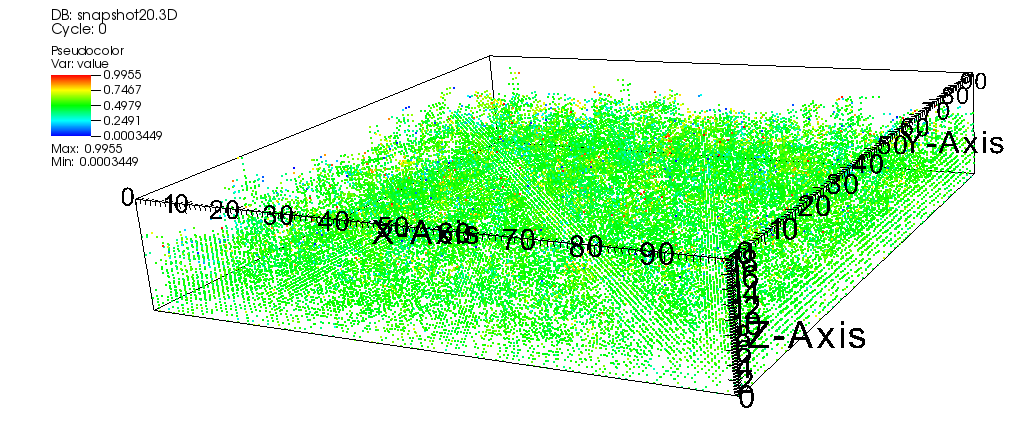
\includegraphics[width=0.8\textwidth]{testBallisticDep1_visit3D.png}}
\end{DoxyImageNoCaption}


A slice of this snapshot in Vis\+It, showing particles with cell index {\itshape j} = 50, should look something like this\+:

 
\begin{DoxyImageNoCaption}
  \mbox{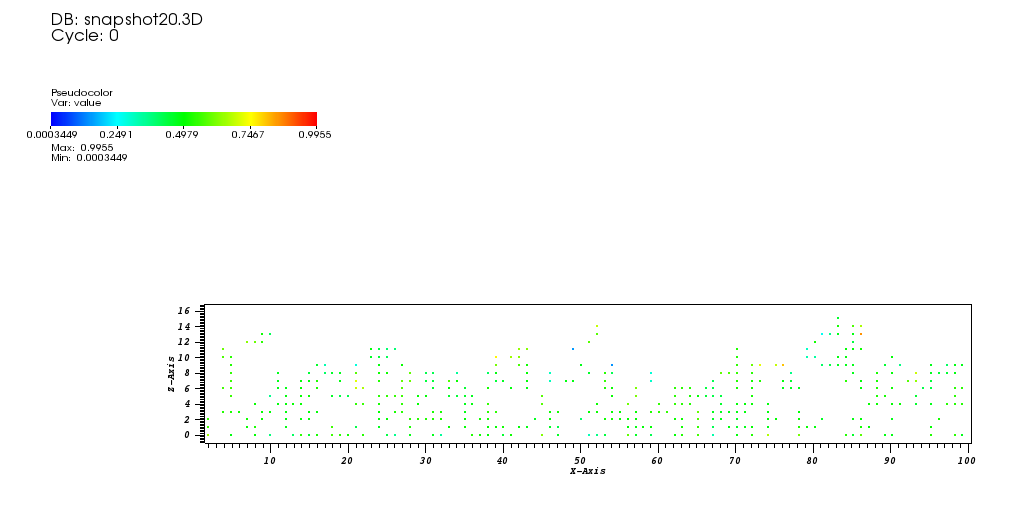
\includegraphics[width=0.8\textwidth]{testBallisticDep1_visit_slice_y50.png}}
\end{DoxyImageNoCaption}
\hypertarget{illustrating_use_by_example_example_baldep_impl2}{}\doxysubsection{\texorpdfstring{Second implementation}{Second implementation}}\label{illustrating_use_by_example_example_baldep_impl2}
One may have noticed a problem with the implementation of ballistic deposition described above. While only the values of the quantity labeled {\ttfamily BDInt\+Val\+::\+ACTIVE\+\_\+\+ZONE\+\_\+\+HEIGHT} in the first lattice plane are used, this quantity is defined for all cells of the lattice, which is somewhat wasteful. In this alternate implementation, then, the values of the auxiliary array $h_a(i,j)$ will be stored not within the first plane of the lattice, but rather in a separate auxiliary array. Also, semi-\/manual tracking will be used for this example. The code for this new implementation is in {\ttfamily doc/example-\/code/test\+Ballistic\+Dep2} of the installation directory of the ARL \doxylink{namespaceKMCThinFilm}{KMCThin\+Film} library.

We begin by defining {\ttfamily Int\+Array2D} in {\ttfamily Events\+And\+Actions.\+hpp}, a type for a two-\/dimensional integer array, using the multi-\/array implementation from Boost \texorpdfstring{$<$}{<}\href{http://www.boost.org}{\texttt{ http\+://www.\+boost.\+org}}\texorpdfstring{$>$}{>}, and a shared pointer for that type, also using a ``smart'' pointer implementation from the Boost library\+:


\begin{DoxyCodeInclude}{0}
\DoxyCodeLine{\textcolor{preprocessor}{\#include\ <boost/multi\_array.hpp>}}
\DoxyCodeLine{\textcolor{preprocessor}{\#include\ <boost/shared\_ptr.hpp>}}
\DoxyCodeLine{}
\DoxyCodeLine{\textcolor{keyword}{typedef}\ boost::multi\_array<int,\ 2>\ IntArray2D;}
\DoxyCodeLine{\textcolor{keyword}{typedef}\ boost::shared\_ptr<IntArray2D>\ IntArray2DSharedPtr;}

\end{DoxyCodeInclude}


In the definition of the function object class performing ballistic deposition,


\begin{DoxyCodeInclude}{0}
\DoxyCodeLine{\textcolor{keyword}{class\ }DepositionExecute\ \{}
\DoxyCodeLine{\textcolor{keyword}{public}:}
\DoxyCodeLine{\ \ DepositionExecute(\textcolor{keyword}{const}\ KMCThinFilm::LatticePlanarBBox\ \&\ planarBBox);}
\DoxyCodeLine{}
\DoxyCodeLine{\ \ \textcolor{keywordtype}{void}\ operator()(\textcolor{keyword}{const}\ KMCThinFilm::CellInds\ \&\ ci,}
\DoxyCodeLine{\ \ \ \ \ \ \ \ \ \ \ \ \ \ \ \ \ \ \textcolor{keyword}{const}\ KMCThinFilm::SimulationState\ \&\ simState,}
\DoxyCodeLine{\ \ \ \ \ \ \ \ \ \ \ \ \ \ \ \ \ \ \textcolor{keyword}{const}\ KMCThinFilm::Lattice\ \&\ lattice,}
\DoxyCodeLine{\ \ \ \ \ \ \ \ \ \ \ \ \ \ \ \ \ \ std::vector<KMCThinFilm::CellsToChange>\ \&\ ctcVec);}
\DoxyCodeLine{\textcolor{keyword}{private}:}
\DoxyCodeLine{\ \ IntArray2DSharedPtr\ activeZoneHeights\_;}
\DoxyCodeLine{}
\DoxyCodeLine{\ \ std::vector<KMCThinFilm::CellIndsOffset>\ neighOffsets\_;}
\DoxyCodeLine{\};}

\end{DoxyCodeInclude}


we have a shared pointer to an {\ttfamily Int\+Array2D} object, {\ttfamily active\+Zone\+Heights\+\_\+}. The constructor takes a \doxylink{structKMCThinFilm_1_1LatticePlanarBBox}{KMCThin\+Film\+::\+Lattice\+Planar\+BBox} parameter object, which is used to size the array to which {\ttfamily active\+Zone\+Heights\+\_\+} points\+:


\begin{DoxyCodeInclude}{0}
\DoxyCodeLine{DepositionExecute::DepositionExecute(\textcolor{keyword}{const}\ \mbox{\hyperlink{structKMCThinFilm_1_1LatticePlanarBBox}{LatticePlanarBBox}}\ \&\ planarBBox)}
\DoxyCodeLine{:\ activeZoneHeights\_(new\ IntArray2D)\ \{}
\DoxyCodeLine{}
\DoxyCodeLine{\ \ \textcolor{comment}{//\ The\ resize()\ member\ function\ will\ initialize\ the\ elements\ of\ this}}
\DoxyCodeLine{\ \ \textcolor{comment}{//\ array\ to\ zero.}}
\DoxyCodeLine{\ \ activeZoneHeights\_-\/>resize(boost::extents[planarBBox.\mbox{\hyperlink{structKMCThinFilm_1_1LatticePlanarBBox_a8bc6629f20496b2845d66f924a04f35a}{imaxP1}}\ -\/\ planarBBox.\mbox{\hyperlink{structKMCThinFilm_1_1LatticePlanarBBox_a9de43623938e1ceb68c26feafd4cd009}{imin}}]}
\DoxyCodeLine{\ \ \ \ \ \ \ \ \ \ \ \ \ \ \ \ \ \ \ \ \ \ \ \ \ \ \ \ \ [planarBBox.\mbox{\hyperlink{structKMCThinFilm_1_1LatticePlanarBBox_abedcda2c34e2bdfe0404e22838ed33dd}{jmaxP1}}\ -\/\ planarBBox.\mbox{\hyperlink{structKMCThinFilm_1_1LatticePlanarBBox_aa227140b560487687496bdbaef79d85e}{jmin}}]);}
\DoxyCodeLine{\ \ }
\DoxyCodeLine{\ \ neighOffsets\_.reserve(4);}
\DoxyCodeLine{\ \ neighOffsets\_.push\_back(\mbox{\hyperlink{classKMCThinFilm_1_1CellIndsOffset}{CellIndsOffset}}(\ 0,-\/1));}
\DoxyCodeLine{\ \ neighOffsets\_.push\_back(\mbox{\hyperlink{classKMCThinFilm_1_1CellIndsOffset}{CellIndsOffset}}(\ 0,+1));}
\DoxyCodeLine{\ \ neighOffsets\_.push\_back(\mbox{\hyperlink{classKMCThinFilm_1_1CellIndsOffset}{CellIndsOffset}}(-\/1,\ 0));}
\DoxyCodeLine{\ \ neighOffsets\_.push\_back(\mbox{\hyperlink{classKMCThinFilm_1_1CellIndsOffset}{CellIndsOffset}}(+1,\ 0));}
\DoxyCodeLine{}
\DoxyCodeLine{\}}

\end{DoxyCodeInclude}


In the driver code {\ttfamily test\+Ballistic\+Dep.\+cpp}, the \doxylink{structKMCThinFilm_1_1LatticePlanarBBox}{KMCThin\+Film\+::\+Lattice\+Planar\+BBox} parameter object passed to this constructor contains the lateral bounds of the global lattice.

Finally, the implementation of ballistic deposition is as follows\+:


\begin{DoxyCodeInclude}{0}
\DoxyCodeLine{\textcolor{keywordtype}{void}\ DepositionExecute::operator()(\textcolor{keyword}{const}\ \mbox{\hyperlink{classKMCThinFilm_1_1CellInds}{KMCThinFilm::CellInds}}\ \&\ ci,}
\DoxyCodeLine{\ \ \ \ \ \ \ \ \ \ \ \ \ \ \ \ \ \ \ \ \ \ \ \ \ \ \ \ \ \ \ \ \ \ \ \textcolor{keyword}{const}\ \mbox{\hyperlink{classKMCThinFilm_1_1SimulationState}{KMCThinFilm::SimulationState}}\ \&\ simState,}
\DoxyCodeLine{\ \ \ \ \ \ \ \ \ \ \ \ \ \ \ \ \ \ \ \ \ \ \ \ \ \ \ \ \ \ \ \ \ \ \ \textcolor{keyword}{const}\ \mbox{\hyperlink{classKMCThinFilm_1_1Lattice}{KMCThinFilm::Lattice}}\ \&\ lattice,}
\DoxyCodeLine{\ \ \ \ \ \ \ \ \ \ \ \ \ \ \ \ \ \ \ \ \ \ \ \ \ \ \ \ \ \ \ \ \ \ \ std::vector<KMCThinFilm::CellsToChange>\ \&\ ctcVec)\ \{}
\DoxyCodeLine{\ \ }
\DoxyCodeLine{\ \ \textcolor{comment}{/*\ Ballistic\ deposition\ algorithm\ for\ cubic\ lattices\ from\ Meakin\ and}}
\DoxyCodeLine{\textcolor{comment}{\ \ \ \ \ Krug,\ Physical\ Review\ A,\ vol.\ 46,\ num.\ 6,\ pp.\ 3390-\/3399\ (1992).*/}}
\DoxyCodeLine{}
\DoxyCodeLine{\ \ \textcolor{keywordtype}{int}\ kDepAtom\ =\ (*activeZoneHeights\_)[ci.i][ci.j];}
\DoxyCodeLine{}
\DoxyCodeLine{\ \ \mbox{\hyperlink{classKMCThinFilm_1_1CellInds}{CellInds}}\ ciTo(ci.i,\ ci.j,\ kDepAtom);}
\DoxyCodeLine{}
\DoxyCodeLine{\ \ \mbox{\hyperlink{classKMCThinFilm_1_1CellsToChange}{CellsToChange}}\ \&\ ctc\ =\ ctcVec[0];}
\DoxyCodeLine{}
\DoxyCodeLine{\ \ ctc.\mbox{\hyperlink{classKMCThinFilm_1_1CellsToChange_a8a56c1106701d5bc3409cd30343fee2c}{setCenter}}(ciTo);}
\DoxyCodeLine{\ \ }
\DoxyCodeLine{\ \ ctc.\mbox{\hyperlink{classKMCThinFilm_1_1CellsToChange_a6753306ace3d33af03814bfb048498b5}{addLatticePlanes}}(ciTo.k\ -\/\ ci.k);}
\DoxyCodeLine{\ \ ctc.\mbox{\hyperlink{classKMCThinFilm_1_1CellsToChange_a62079b840cc200e37e2907ba2e394f78}{setInt}}(0,\ BDIntVal::IS\_OCCUPIED,\ 1);}
\DoxyCodeLine{}
\DoxyCodeLine{\ \ \textcolor{keywordflow}{for}\ (std::vector<CellIndsOffset>::const\_iterator\ offsetItr\ =\ neighOffsets\_.begin(),}
\DoxyCodeLine{\ \ \ \ \ \ \ \ \ offsetItrEnd\ =\ neighOffsets\_.end();\ offsetItr\ !=\ offsetItrEnd;\ ++offsetItr)\ \{}
\DoxyCodeLine{}
\DoxyCodeLine{\ \ \ \ \mbox{\hyperlink{classKMCThinFilm_1_1CellInds}{CellInds}}\ neigh\ =\ ciTo\ +\ *offsetItr;}
\DoxyCodeLine{}
\DoxyCodeLine{\ \ \ \ \textcolor{keywordtype}{int}\ i\ =\ lattice.\mbox{\hyperlink{classKMCThinFilm_1_1Lattice_ad86c9013774b072638db5527ced49cf8}{wrapI}}(neigh);}
\DoxyCodeLine{\ \ \ \ \textcolor{keywordtype}{int}\ j\ =\ lattice.\mbox{\hyperlink{classKMCThinFilm_1_1Lattice_a837c173e46cb56875b02dbdb27da71c9}{wrapJ}}(neigh);}
\DoxyCodeLine{}
\DoxyCodeLine{\ \ \ \ \textcolor{keywordflow}{if}\ ((*activeZoneHeights\_)[i][j]\ <\ kDepAtom)\ \{}
\DoxyCodeLine{\ \ \ \ \ \ (*activeZoneHeights\_)[i][j]\ =\ kDepAtom;}
\DoxyCodeLine{\ \ \ \ \}}
\DoxyCodeLine{\ \ \}}
\DoxyCodeLine{}
\DoxyCodeLine{\ \ ++((*activeZoneHeights\_)[ci.i][ci.j]);}
\DoxyCodeLine{\}}

\end{DoxyCodeInclude}


Note that since {\ttfamily active\+Zone\+Heights\+\_\+} is an external array, we use \doxylink{classKMCThinFilm_1_1Lattice_ad86c9013774b072638db5527ced49cf8}{KMCThin\+Film\+::\+Lattice\+::wrap\+I()} and \doxylink{classKMCThinFilm_1_1Lattice_a837c173e46cb56875b02dbdb27da71c9}{KMCThin\+Film\+::\+Lattice\+::wrap\+J()} to ensure that the array indices used with {\ttfamily active\+Zone\+Heights\+\_\+} are correctly wrapped to account for periodic boundary conditions. This was not necessary when $h_a(i,j)$ was stored in the first plane of the lattice and \doxylink{classKMCThinFilm_1_1Lattice_aff659b471f414c579a51fe280b218ef1}{KMCThin\+Film\+::\+Lattice\+::get\+Int()} was used to access its contents, since \doxylink{classKMCThinFilm_1_1Lattice_aff659b471f414c579a51fe280b218ef1}{get\+Int()} automatically accounts for any periodic boundary conditions. Also, since semi-\/manual tracking is used, {\ttfamily lattice} is a {\itshape constant} reference, so planes must be added to the lattice via the member function \doxylink{classKMCThinFilm_1_1CellsToChange_a6753306ace3d33af03814bfb048498b5}{KMCThin\+Film\+::\+Cells\+To\+Change\+::add\+Lattice\+Planes()}.

One may ask why {\ttfamily active\+Zone\+Heights\+\_\+} is a pointer to an array instead of just an array. The reason for this is that when the {\ttfamily Deposition\+Execute} object is passed to \doxylink{classKMCThinFilm_1_1Simulation_affa3dff53afd248546457944b98376d9}{KMCThin\+Film\+::\+Simulation\+::add\+Over\+Lattice\+Event()}, it is passed by value. This would mean that there would be two copies of the {\ttfamily active\+Zone\+Heights\+\_\+} array, one created when the {\ttfamily Deposition\+Execute} object is constructed, and another when a copy of this object is made to pass it by value. By using a pointer, only a pointer to the array is copied. A ``smart'' shared pointer is used so that it will automatically be deleted when there are no more references to it.

One downside of this implementation is that it is more difficult to parallelize than the previous one. With {\ttfamily \texorpdfstring{$\ast$}{*}active\+Zone\+Heights\+\_\+} as a separate array, the process of splitting up the array, taking care of updates of ghost entries, etc. has to be handled explicitly. The handling of MPI communication could be done via a periodic action executed at each step, though one would need to refactor the code so that a {\ttfamily Deposition\+Execute} object and the function object performing the periodic action could both access the array containing $h_a(i,j)$.

The resulting simulated thin film produced by this implementation is similar to that produced in the previous simulation but not the same, even if the same seed to the random number generator has been used. This is because the previous implementation contains calls to {\ttfamily lattice.\+set\+Int(..., BDInt\+Val\+::\+ACTIVE\+\_\+\+ZONE\+\_\+\+HEIGHT, ...)} in the function object that executes a deposition event. This triggers the solvers in the simulation to examine the possible events in the neighborhood of where the value of the quantity labeled {\ttfamily BDInt\+Val\+::\+ACTIVE\+\_\+\+ZONE\+\_\+\+HEIGHT} has been changed, which, due to implementation details in the ARL \doxylink{namespaceKMCThinFilm}{KMCThin\+Film} library, ends up changing the order that possible events with the same propensity are stored, which in turn affects which event is randomly chosen at a time step.\hypertarget{illustrating_use_by_example_example_pat_sub}{}\doxysection{\texorpdfstring{Example\+: Implementations of a patterned substrate model}{Example\+: Implementations of a patterned substrate model}}\label{illustrating_use_by_example_example_pat_sub}
This example is meant to show how the ARL \doxylink{namespaceKMCThinFilm}{KMCThin\+Film} library may be used to implement models that are unusual in the sense that they have features that would almost inevitably require custom code to implement. An example of such a model is that of a patterned substrate \cite{kur99}. Like the fractal model, they use solid-\/on-\/solid modeling of a cubic lattice, which again means that the arrangement of atoms in the actual true lattice can be stored in a two-\/dimensional computational lattice, such that $(i,j,0)$ in the computational lattice stores the height of the column of particles at $(i,j,0)$ in the true lattice. As before, if a diffusing particle in the true lattice moves to a nearest-\/neighboring site that is not just above another particle, then the diffusing particle will fall until it lands on top of another particle. Also, if the site to which a particle attempts to move is occupied, then the particle will climb to the top of the column of particles that contains that occupied site. Falling and climbing are illustrated below, where an empty circle indicates the old position of a particle and a dark filled circle indicates the new position of a particle\+:

 
\begin{DoxyImageNoCaption}
  \mbox{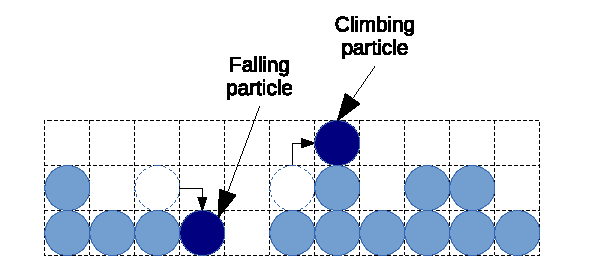
\includegraphics[height=1.5in]{FallingAndClimbingParticles}}
\end{DoxyImageNoCaption}


In one of the models of Kuronen et al., the propensity for the hopping of a particle at a lattice cell is   \[p = k\exp\left(-\frac{E}{k_B T}\right)
\] where $k_B$ is the Boltzmann constant, {\itshape T} is temperature, $k = kT/h$ with {\itshape h} being Planck\textquotesingle{}s constant, and   \[E = E_s(i,j) + n E_n
\] Here, {\itshape n} is the number of occupied lateral neighbors of the cell, $E_n$ (= 0.\+18 eV) is a measure of the bond strength between a particle and a lateral nearest neighboring particle, and $E_s$ is a position-\/dependent diffusion barrier dependent on the patterning of the substrate, which varies with {\itshape i} and {\itshape j} as illustrated below, with brighter colors indicating higher values.

 
\begin{DoxyImageNoCaption}
  \mbox{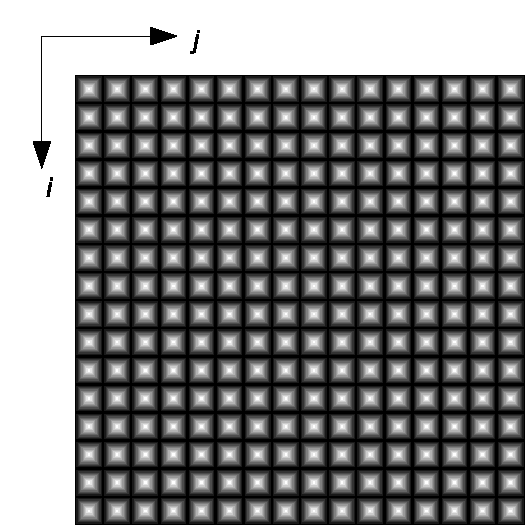
\includegraphics[height=3in]{tiled16x16Domain_annotated}}
\end{DoxyImageNoCaption}


The above pattern consists of a 16 {$\times$} 16 array of square domains, and each domain is an array of 22 {$\times$} 22 elements. This implies that the lattice has lateral dimensions (16{$\cdot$}22) {$\times$} (16{$\cdot$}22). At the edge of a domain, $E_s$ is at its minimum value, 0.\+65 eV, and at the center of a domain, it is at its maximum, 0.\+85 eV. $E_s$ varies linearly between its minimum and maximum values.

The results of this patterned substrate model should be an arrangement of islands centered about the parts of the substrate where $E_s$ is maximum.\hypertarget{illustrating_use_by_example_example_pat_sub_impl1}{}\doxysubsection{\texorpdfstring{First implementation}{First implementation}}\label{illustrating_use_by_example_example_pat_sub_impl1}
The code for this implementation is in {\ttfamily doc/example-\/code/test\+Patterned\+Surface1} of the installation directory of the ARL \doxylink{namespaceKMCThinFilm}{KMCThin\+Film} library. In it, the value $E_s(i,j)$ is stored at cell $(i,j,0)$ of the computational lattice. This requires using a special method to initialize the lattice. The values of $E_s(i,j)$ are stored in a file (entitled {\ttfamily tiled16x16\+Domain.\+dat}) where the first line contains the lateral dimensions of the lattice and subsequent lines are of the form

\begin{DoxyVerb}i j E_s(i,j)
\end{DoxyVerb}


where the first two numbers in the line are the lateral lattice cell indices and the third number is the value of $E_s$ for those indices.

We begin with the files {\ttfamily Init\+Lattice.\+hpp} and {\ttfamily Init\+Lattice.\+cpp}, which contain the definition and implementation of the function object than initializes the lattice. The contents of the first file are


\begin{DoxyCodeInclude}{0}
\DoxyCodeLine{\textcolor{preprocessor}{\#ifndef\ INIT\_LATTICE\_HPP}}
\DoxyCodeLine{\textcolor{preprocessor}{\#define\ INIT\_LATTICE\_HPP}}
\DoxyCodeLine{}
\DoxyCodeLine{\textcolor{preprocessor}{\#include\ <string>}}
\DoxyCodeLine{}
\DoxyCodeLine{\textcolor{preprocessor}{\#include\ <KMCThinFilm/Lattice.hpp>}}
\DoxyCodeLine{\textcolor{preprocessor}{\#include\ <KMCThinFilm/ErrorHandling.hpp>}}
\DoxyCodeLine{}
\DoxyCodeLine{\textcolor{keyword}{class\ }InitLatticeFromFile\ \{}
\DoxyCodeLine{\textcolor{keyword}{public}:}
\DoxyCodeLine{\ \ InitLatticeFromFile(\textcolor{keyword}{const}\ std::string\ \&\ inpFName)}
\DoxyCodeLine{\ \ \ \ :\ inpFName\_(inpFName)}
\DoxyCodeLine{\ \ \{\}}
\DoxyCodeLine{}
\DoxyCodeLine{\ \ \textcolor{keywordtype}{void}\ operator()(KMCThinFilm::Lattice\ \&\ lattice)\ \textcolor{keyword}{const};}
\DoxyCodeLine{\textcolor{keyword}{private}:}
\DoxyCodeLine{\ \ std::string\ inpFName\_;}
\DoxyCodeLine{\};}
\DoxyCodeLine{}
\DoxyCodeLine{\textcolor{preprocessor}{\#endif\ }\textcolor{comment}{/*\ INIT\_LATTICE\_HPP\ */}\textcolor{preprocessor}{}}

\end{DoxyCodeInclude}


The constructor of the {\ttfamily Init\+Lattice\+From\+File} class here takes as an argument the name of the input file containing the values of $E_s$. The contents of {\ttfamily Init\+Lattice.\+cpp} are as follows\+:


\begin{DoxyCodeInclude}{0}
\DoxyCodeLine{\textcolor{preprocessor}{\#include\ "{}InitLattice.hpp"{}}}
\DoxyCodeLine{\textcolor{preprocessor}{\#include\ "{}EventsAndActions.hpp"{}}}
\DoxyCodeLine{}
\DoxyCodeLine{\textcolor{preprocessor}{\#include\ <fstream>}}
\DoxyCodeLine{}
\DoxyCodeLine{\textcolor{preprocessor}{\#include\ <boost/array.hpp>}}
\DoxyCodeLine{\textcolor{preprocessor}{\#include\ <boost/lexical\_cast.hpp>}}
\DoxyCodeLine{}
\DoxyCodeLine{\textcolor{keyword}{using\ namespace\ }\mbox{\hyperlink{namespaceKMCThinFilm}{KMCThinFilm}};}
\DoxyCodeLine{}
\DoxyCodeLine{\textcolor{keywordtype}{void}\ InitLatticeFromFile::operator()(\mbox{\hyperlink{classKMCThinFilm_1_1Lattice}{Lattice}}\ \&\ lattice)\textcolor{keyword}{\ const\ }\{}
\DoxyCodeLine{\ \ }
\DoxyCodeLine{\ \ std::ifstream\ inpFile(inpFName\_.c\_str());}
\DoxyCodeLine{}
\DoxyCodeLine{\ \ boost::array<int,2>\ globalPlanarDims;}
\DoxyCodeLine{}
\DoxyCodeLine{\ \ inpFile\ >>\ globalPlanarDims[0]\ >>\ globalPlanarDims[1];}
\DoxyCodeLine{}
\DoxyCodeLine{\ \ \mbox{\hyperlink{structKMCThinFilm_1_1LatticePlanarBBox}{LatticePlanarBBox}}\ globalPlanarBBox;}
\DoxyCodeLine{\ \ lattice.\mbox{\hyperlink{classKMCThinFilm_1_1Lattice_ac160d406b29dc80fb72551ad3d74ac3a}{getGlobalPlanarBBox}}(globalPlanarBBox);}
\DoxyCodeLine{}
\DoxyCodeLine{\ \ \mbox{\hyperlink{namespaceKMCThinFilm_acb9484dffdfd1584121f8a7c8bb8d924}{exitOnCondition}}((globalPlanarDims[0]\ !=\ (globalPlanarBBox.\mbox{\hyperlink{structKMCThinFilm_1_1LatticePlanarBBox_a8bc6629f20496b2845d66f924a04f35a}{imaxP1}}\ -\/\ globalPlanarBBox.\mbox{\hyperlink{structKMCThinFilm_1_1LatticePlanarBBox_a9de43623938e1ceb68c26feafd4cd009}{imin}}))\ ||}
\DoxyCodeLine{\ \ \ \ \ \ \ \ \ \ \ \ \ \ \ \ \ \ (globalPlanarDims[1]\ !=\ (globalPlanarBBox.\mbox{\hyperlink{structKMCThinFilm_1_1LatticePlanarBBox_abedcda2c34e2bdfe0404e22838ed33dd}{jmaxP1}}\ -\/\ globalPlanarBBox.\mbox{\hyperlink{structKMCThinFilm_1_1LatticePlanarBBox_aa227140b560487687496bdbaef79d85e}{jmin}})),}
\DoxyCodeLine{\ \ \ \ \ \ \ \ \ \ \ \ \ \ \ \ \ \ \textcolor{stringliteral}{"{}Mismatch\ in\ lattice\ dimensions\ and\ dimensions\ of\ strain\ eng.\ den.\ array."{}});}
\DoxyCodeLine{}
\DoxyCodeLine{\ \ lattice.\mbox{\hyperlink{classKMCThinFilm_1_1Lattice_aa36bda22ed2b0bc8d8737d3d63009765}{addPlanes}}(1);}
\DoxyCodeLine{}
\DoxyCodeLine{\ \ \mbox{\hyperlink{structKMCThinFilm_1_1LatticePlanarBBox}{LatticePlanarBBox}}\ localPlanarBBox;}
\DoxyCodeLine{\ \ lattice.\mbox{\hyperlink{classKMCThinFilm_1_1Lattice_a1504ff860e046a8965b37dd437a74c52}{getLocalPlanarBBox}}(\textcolor{keyword}{false},\ localPlanarBBox);}
\DoxyCodeLine{}
\DoxyCodeLine{\ \ \textcolor{keywordtype}{int}\ maxLineNumP1\ =\ (globalPlanarDims[0])*(globalPlanarDims[1]);}
\DoxyCodeLine{}
\DoxyCodeLine{\ \ \mbox{\hyperlink{classKMCThinFilm_1_1CellInds}{CellInds}}\ ci;\ ci.k\ =\ 0;}
\DoxyCodeLine{\ \ \textcolor{keywordflow}{for}\ (\textcolor{keywordtype}{int}\ lineNum\ =\ 0;\ lineNum\ <\ maxLineNumP1;\ ++lineNum)\ \{}
\DoxyCodeLine{\ \ \ \ }
\DoxyCodeLine{\ \ \ \ \textcolor{keywordtype}{int}\ i,\ j;}
\DoxyCodeLine{\ \ \ \ \textcolor{keywordtype}{double}\ E\_s;}
\DoxyCodeLine{}
\DoxyCodeLine{\ \ \ \ inpFile\ >>\ i\ >>\ j\ >>\ E\_s;}
\DoxyCodeLine{}
\DoxyCodeLine{\ \ \ \ \textcolor{keywordflow}{if}\ ((i\ >=\ localPlanarBBox.\mbox{\hyperlink{structKMCThinFilm_1_1LatticePlanarBBox_a9de43623938e1ceb68c26feafd4cd009}{imin}})\ \&\&\ (i\ <\ localPlanarBBox.\mbox{\hyperlink{structKMCThinFilm_1_1LatticePlanarBBox_a8bc6629f20496b2845d66f924a04f35a}{imaxP1}})\ \&\&\ }
\DoxyCodeLine{\ \ \ \ \ \ \ \ (j\ >=\ localPlanarBBox.\mbox{\hyperlink{structKMCThinFilm_1_1LatticePlanarBBox_aa227140b560487687496bdbaef79d85e}{jmin}})\ \&\&\ (j\ <\ localPlanarBBox.\mbox{\hyperlink{structKMCThinFilm_1_1LatticePlanarBBox_abedcda2c34e2bdfe0404e22838ed33dd}{jmaxP1}}))\ \{}
\DoxyCodeLine{}
\DoxyCodeLine{\ \ \ \ \ \ ci.i\ =\ i;}
\DoxyCodeLine{\ \ \ \ \ \ ci.j\ =\ j;}
\DoxyCodeLine{\ \ \ \ \ \ \ \ }
\DoxyCodeLine{\ \ \ \ \ \ lattice.\mbox{\hyperlink{classKMCThinFilm_1_1Lattice_aefe9601bf62fdb46d451d61fa017e691}{setFloat}}(ci,\ PSFloatVal::E\_s,\ E\_s);}
\DoxyCodeLine{\ \ \ \ \}}
\DoxyCodeLine{}
\DoxyCodeLine{\ \ \}}
\DoxyCodeLine{\ \ \ \ }
\DoxyCodeLine{\ \ inpFile.close();}
\DoxyCodeLine{}
\DoxyCodeLine{\}}

\end{DoxyCodeInclude}


This operator reads in the file containing the values of $E_s(i,j)$, line by line, and stores these values in the floating-\/point array element labeled {\ttfamily PSFloat\+Val\+::\+E\+\_\+s} in lattice cell $(i,j,0)$. The (global) lateral bounds of the lattice have already been initialized before this operator has even been invoked, so here there is a check to ensure that the lateral bounds of the lattice indicated in the first line of the file match the actual lateral bounds of the lattice. After this check, the actual initialization begins. First, a lattice plane is added with the \doxylink{classKMCThinFilm_1_1Lattice_aa36bda22ed2b0bc8d8737d3d63009765}{KMCThin\+Film\+::\+Lattice\+::add\+Planes()} member function. Shortly afterward comes the reading in of the rest of the file containing the values of $E_s(i,j)$. There is some allowance for parallel implementation. The local bounds of indices {\itshape i} and {\itshape j} are determined using \doxylink{classKMCThinFilm_1_1Lattice_a1504ff860e046a8965b37dd437a74c52}{KMCThin\+Film\+::\+Lattice\+::get\+Local\+Planar\+BBox}. While each MPI process would still read in the whole file, which is not that efficient, the process would also only store the values of $E_s(i,j)$ for the lattice cell indices {\itshape i} and {\itshape j} whose values are within the previously determined local bounds.

In the driver file {\ttfamily test\+Patterned\+Surface.\+cpp}, the simulation is initialized as follows\+:


\begin{DoxyCodeInclude}{0}
\DoxyCodeLine{\ \ \mbox{\hyperlink{structKMCThinFilm_1_1LatticeParams}{LatticeParams}}\ latParams;}
\DoxyCodeLine{\ \ latParams.\mbox{\hyperlink{structKMCThinFilm_1_1LatticeParams_a7a9d46d27758a276fd20d9c18156371a}{numIntsPerCell}}\ =\ PSIntVal::SIZE;}
\DoxyCodeLine{\ \ latParams.\mbox{\hyperlink{structKMCThinFilm_1_1LatticeParams_a55263f7f4ef826b814ffeaae27ddf687}{numFloatsPerCell}}\ =\ PSFloatVal::SIZE;}
\DoxyCodeLine{}
\DoxyCodeLine{\ \ std::ifstream\ patternFile(patternFName.c\_str());}
\DoxyCodeLine{}
\DoxyCodeLine{\ \ \textcolor{keywordflow}{if}\ (patternFile)\ \{}
\DoxyCodeLine{\ \ \ \ patternFile\ >>\ latParams.\mbox{\hyperlink{structKMCThinFilm_1_1LatticeParams_a3a3cc62a6fb5fdda00ed2c63e1ff1020}{globalPlanarDims}}[0]\ >>\ latParams.\mbox{\hyperlink{structKMCThinFilm_1_1LatticeParams_a3a3cc62a6fb5fdda00ed2c63e1ff1020}{globalPlanarDims}}[1];}
\DoxyCodeLine{\ \ \}}
\DoxyCodeLine{\ \ \textcolor{keywordflow}{else}\ \{}
\DoxyCodeLine{\ \ \ \ \mbox{\hyperlink{namespaceKMCThinFilm_a77bd0cec2abe3a269140d80cfea34ed8}{exitWithMsg}}(\textcolor{stringliteral}{"{}Cannot\ access\ "{}}\ +\ patternFName\ +\ }
\DoxyCodeLine{\ \ \ \ \ \ \ \ \ \ \ \ \ \ \ \ \textcolor{stringliteral}{"{}.\ Check\ if\ your\ are\ executing\ this\ program\ from\ the\ correct\ directory."{}});}
\DoxyCodeLine{\ \ \}}
\DoxyCodeLine{}
\DoxyCodeLine{\ \ patternFile.close();}
\DoxyCodeLine{}
\DoxyCodeLine{\ \ latParams.\mbox{\hyperlink{structKMCThinFilm_1_1LatticeParams_a3591118c88951f3a6c7de54117979c36}{latInit}}\ =\ InitLatticeFromFile(patternFName);}
\DoxyCodeLine{}
\DoxyCodeLine{\ \ \mbox{\hyperlink{classKMCThinFilm_1_1Simulation}{Simulation}}\ sim(latParams);}

\end{DoxyCodeInclude}


Here, {\ttfamily pattern\+FName} is the name of the file containing the values of $E_s(i,j)$. The first line of this file is read in to determine the lateral dimensions of the lattice, and then the file is closed. Afterwards, the {\itshape lat\+Init} member of the \doxylink{structKMCThinFilm_1_1LatticeParams}{KMCThin\+Film\+::\+Lattice\+Params} parameter object is set to an instance of the {\ttfamily Init\+Lattice\+From\+File} class, which is of course initialized to read from the file with the name {\ttfamily pattern\+FName}. (This also means that this implementation is a bit inelegant, since part of the file {\ttfamily pattern\+FName} will be read twice.)

This takes care of the initialization of the lattice.

Deposition here is done by the same means as in the example of the fractal solid-\/on-\/solid model using auto-\/tracking, while the execution of a hopping event is done by the same means as in the example of the fractal solid-\/on-\/solid model using semi-\/manual tracking. It is mainly the determination of a hopping event\textquotesingle{}s propensity that is different. The definition of the function object class for determining propensity of hopping is shown below\+:


\begin{DoxyCodeInclude}{0}
\DoxyCodeLine{\textcolor{keyword}{class\ }HoppingPropensity\ \{}
\DoxyCodeLine{\textcolor{keyword}{public}:}
\DoxyCodeLine{\ \ HoppingPropensity(\textcolor{keywordtype}{double}\ E\_n,\ \textcolor{keywordtype}{double}\ T)\ }
\DoxyCodeLine{\ \ \ \ :\ E\_n\_(E\_n),\ kBT\_(PhysConst::kB*T),\ k\_(kBT\_/PhysConst::h)}
\DoxyCodeLine{\ \ \{\}}
\DoxyCodeLine{\ \ \textcolor{keywordtype}{void}\ operator()(\textcolor{keyword}{const}\ KMCThinFilm::CellNeighProbe\ \&\ cnp,}
\DoxyCodeLine{\ \ \ \ \ \ \ \ \ \ \ \ \ \ \ \ \ \ std::vector<double>\ \&\ propensityVec)\ \textcolor{keyword}{const};}
\DoxyCodeLine{\textcolor{keyword}{private}:}
\DoxyCodeLine{\ \ \textcolor{keywordtype}{double}\ E\_n\_,\ kBT\_,\ k\_;}
\DoxyCodeLine{\};}

\end{DoxyCodeInclude}


The constants {\ttfamily Phys\+Const\+::kB} and {\ttfamily Phys\+Const\+::h} are merely the Boltzmann constant and Planck\textquotesingle{}s constant, and they are defined in the file {\ttfamily Physical\+Constants.\+hpp} of this example code. The private variables {\ttfamily E\+\_\+n\+\_\+}, {\ttfamily k\+BT\+\_\+}, and {\ttfamily k\+\_\+} correspond to the aforementioned expressions $E_n$, $k_B T$, and {\itshape k}. The implementation of the function object class for determining hopping propensity is shown below\+:


\begin{DoxyCodeInclude}{0}
\DoxyCodeLine{\textcolor{keywordtype}{void}\ HoppingPropensity::operator()(\textcolor{keyword}{const}\ \mbox{\hyperlink{classKMCThinFilm_1_1CellNeighProbe}{CellNeighProbe}}\ \&\ cnp,}
\DoxyCodeLine{\ \ \ \ \ \ \ \ \ \ \ \ \ \ \ \ \ \ \ \ \ \ \ \ \ \ \ \ \ \ \ \ \ \ \ std::vector<double>\ \&\ propensityVec)\textcolor{keyword}{\ const\ }\{}
\DoxyCodeLine{}
\DoxyCodeLine{\ \ \mbox{\hyperlink{classKMCThinFilm_1_1CellToProbe}{KMCThinFilm::CellToProbe}}\ ctpSelf\ =\ cnp.\mbox{\hyperlink{classKMCThinFilm_1_1CellNeighProbe_a1ba997186f6326b525dd66df4254d198}{getCellToProbe}}(HopOffset::SELF);}
\DoxyCodeLine{}
\DoxyCodeLine{\ \ \textcolor{keywordtype}{int}\ currHeight\ =\ cnp.\mbox{\hyperlink{classKMCThinFilm_1_1CellNeighProbe_a7be3ba45264054167a243f15a1954b92}{getInt}}(ctpSelf,\ PSIntVal::HEIGHT);}
\DoxyCodeLine{}
\DoxyCodeLine{\ \ \textcolor{keywordflow}{if}\ (currHeight\ >\ 0)\ \{}
\DoxyCodeLine{\ \ \ \ }
\DoxyCodeLine{\ \ \ \ \textcolor{keywordtype}{int}\ n\ =\ 0;}
\DoxyCodeLine{}
\DoxyCodeLine{\ \ \ \ \textcolor{keywordflow}{if}\ (cnp.\mbox{\hyperlink{classKMCThinFilm_1_1CellNeighProbe_a7be3ba45264054167a243f15a1954b92}{getInt}}(cnp.\mbox{\hyperlink{classKMCThinFilm_1_1CellNeighProbe_a1ba997186f6326b525dd66df4254d198}{getCellToProbe}}(HopOffset::UP),\ PSIntVal::HEIGHT)\ >=\ currHeight)\ \{}
\DoxyCodeLine{\ \ \ \ \ \ ++n;}
\DoxyCodeLine{\ \ \ \ \}}
\DoxyCodeLine{}
\DoxyCodeLine{\ \ \ \ \textcolor{keywordflow}{if}\ (cnp.\mbox{\hyperlink{classKMCThinFilm_1_1CellNeighProbe_a7be3ba45264054167a243f15a1954b92}{getInt}}(cnp.\mbox{\hyperlink{classKMCThinFilm_1_1CellNeighProbe_a1ba997186f6326b525dd66df4254d198}{getCellToProbe}}(HopOffset::DOWN),\ PSIntVal::HEIGHT)\ >=\ currHeight)\ \{}
\DoxyCodeLine{\ \ \ \ \ \ ++n;}
\DoxyCodeLine{\ \ \ \ \}}
\DoxyCodeLine{}
\DoxyCodeLine{\ \ \ \ \textcolor{keywordflow}{if}\ (cnp.\mbox{\hyperlink{classKMCThinFilm_1_1CellNeighProbe_a7be3ba45264054167a243f15a1954b92}{getInt}}(cnp.\mbox{\hyperlink{classKMCThinFilm_1_1CellNeighProbe_a1ba997186f6326b525dd66df4254d198}{getCellToProbe}}(HopOffset::LEFT),\ PSIntVal::HEIGHT)\ >=\ currHeight)\ \{}
\DoxyCodeLine{\ \ \ \ \ \ ++n;}
\DoxyCodeLine{\ \ \ \ \}}
\DoxyCodeLine{}
\DoxyCodeLine{\ \ \ \ \textcolor{keywordflow}{if}\ (cnp.\mbox{\hyperlink{classKMCThinFilm_1_1CellNeighProbe_a7be3ba45264054167a243f15a1954b92}{getInt}}(cnp.\mbox{\hyperlink{classKMCThinFilm_1_1CellNeighProbe_a1ba997186f6326b525dd66df4254d198}{getCellToProbe}}(HopOffset::RIGHT),\ PSIntVal::HEIGHT)\ >=\ currHeight)\ \{}
\DoxyCodeLine{\ \ \ \ \ \ ++n;}
\DoxyCodeLine{\ \ \ \ \}}
\DoxyCodeLine{}
\DoxyCodeLine{\ \ \ \ \textcolor{keywordtype}{double}\ E\ =\ cnp.\mbox{\hyperlink{classKMCThinFilm_1_1CellNeighProbe_a1425c18df394e394b7c50e9f332371fc}{getFloat}}(ctpSelf,\ PSFloatVal::E\_s)\ +\ n*E\_n\_;}
\DoxyCodeLine{}
\DoxyCodeLine{\ \ \ \ \textcolor{keywordtype}{double}\ p\ =\ k\_*std::exp(-\/E/kBT\_);}
\DoxyCodeLine{\ \ \ \ }
\DoxyCodeLine{\ \ \ \ \textcolor{keywordflow}{for}\ (\textcolor{keywordtype}{int}\ i\ =\ 0;\ i\ <\ PSCellCenteredEvents::SIZE;\ ++i)\ \{}
\DoxyCodeLine{\ \ \ \ \ \ propensityVec[i]\ =\ p;}
\DoxyCodeLine{\ \ \ \ \}}
\DoxyCodeLine{}
\DoxyCodeLine{\ \ \}}
\DoxyCodeLine{\}}

\end{DoxyCodeInclude}


Here, {\ttfamily curr\+Height} is the height of the column of particles at $(\mathtt{ci.i}, \mathtt{ci.j}, 0)$ in the true lattice. Let $(i_{\mathrm{off}}, j_{\mathrm{off}})$ be an offset of cell indices, which for {\ttfamily Hop\+Offset\+::\+UP} is $(0,+1)$, for {\ttfamily Hop\+Offset\+::\+DOWN} is $(0,-1)$, for {\ttfamily Hop\+Offset\+::\+LEFT} is $(-1,0)$, and for {\ttfamily Hop\+Offset\+::\+RIGHT} is $(+1,0)$. If a column of particles at  $(\mathtt{ci.i} + i_{\mathrm{off}}, \mathtt{ci.j} +
j_{\mathrm{off}}, 0)$ is greater than or equal to {\ttfamily curr\+Height}, that means that the site $(\mathtt{ci.i}, \mathtt{ci.j}, \mathtt{currHeight} - 1)$ in the true lattice has an occupied nearest neighbor at  $(\mathtt{ci.i} + i_{\mathrm{off}}, \mathtt{ci.j} +
j_{\mathrm{off}}, \mathtt{currHeight} - 1)$, and the variable {\ttfamily n} is incremented accordingly. The calculation of the propensity, then, follows straightforwardly from the aforementioned formulas for the patterned substrate \cite{kur99}.

An overhead view of the surface of the islands on the patterned substrate at various simulation times {\itshape t}, from 2.\+27 units to its maximum value of 50.\+0 units, is shown below.

 
\begin{DoxyImageNoCaption}
  \mbox{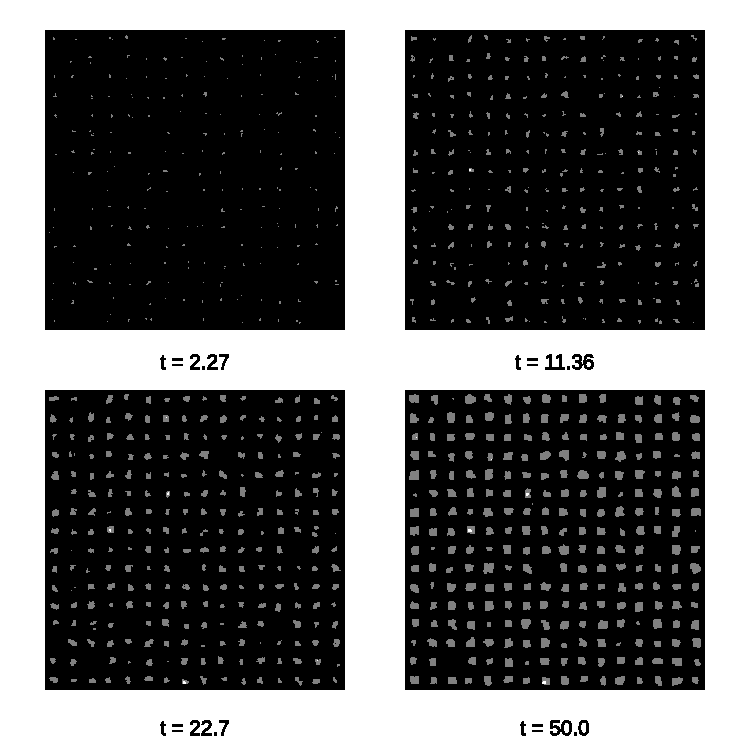
\includegraphics[width=5in]{testPatSubSnapshots}}
\end{DoxyImageNoCaption}
\hypertarget{illustrating_use_by_example_example_pat_sub_impl2}{}\doxysubsection{\texorpdfstring{Second implementation}{Second implementation}}\label{illustrating_use_by_example_example_pat_sub_impl2}
The previous implementation of the patterned substrate model \cite{kur99} does not take advantage of the periodicity of $E_s$. This new implementation will. Instead of storing values of $E_s(i,j)$ in the computational lattice itself, they will be stored in a small array used by the function object used to calculate propensities. This means that no special means to initialize the lattice is required. The code for this implementation is in {\ttfamily doc/example-\/code/test\+Patterned\+Surface2} of the installation directory of the ARL \doxylink{namespaceKMCThinFilm}{KMCThin\+Film} library.

The file containing the values of $E_s(i,j)$, {\ttfamily single\+Domain.\+dat} only contains the values of $E_s$ within a single domain of (22 {$\times$} 22 array) elements. The first line of this file contains the dimensions of this domain, and the rest of the lines in this file have the following format,

\begin{DoxyVerb}i j E_s(i,j)
\end{DoxyVerb}


where the first two numbers in the line are the indices of the domain array and the third number is the value of $E_s$ for those indices. In the driver code {\ttfamily test\+Patterned\+Surface.\+cpp}, this file is read into an array as follows,


\begin{DoxyCodeInclude}{0}
\DoxyCodeLine{\ \ DblArray2D\ E\_s;}
\DoxyCodeLine{\ \ }
\DoxyCodeLine{\ \ std::ifstream\ patternFile(\textcolor{stringliteral}{"{}../singleDomain.dat"{}});}
\DoxyCodeLine{\ \ boost::array<int,2>\ E\_s\_extents;}
\DoxyCodeLine{}
\DoxyCodeLine{\ \ patternFile\ >>\ E\_s\_extents[0]\ >>\ E\_s\_extents[1];}
\DoxyCodeLine{\ \ E\_s.resize(E\_s\_extents);}
\DoxyCodeLine{}
\DoxyCodeLine{\ \ \textcolor{keywordtype}{int}\ E\_s\_i,\ E\_s\_j;}
\DoxyCodeLine{\ \ \textcolor{keywordtype}{double}\ E\_s\_val;}
\DoxyCodeLine{}
\DoxyCodeLine{\ \ \textcolor{keywordflow}{while}\ (patternFile\ >>\ E\_s\_i\ >>\ E\_s\_j\ >>\ E\_s\_val)\ \{}
\DoxyCodeLine{\ \ \ \ E\_s[E\_s\_i][E\_s\_j]\ =\ E\_s\_val;}
\DoxyCodeLine{\ \ \}}

\end{DoxyCodeInclude}


where {\ttfamily Dbl\+Array2D} is defined in {\ttfamily Events\+And\+Actions.\+hpp} as


\begin{DoxyCodeInclude}{0}
\DoxyCodeLine{\textcolor{preprocessor}{\#include\ <boost/multi\_array.hpp>}}
\DoxyCodeLine{\textcolor{keyword}{typedef}\ boost::multi\_array<double,2>\ DblArray2D;}

\end{DoxyCodeInclude}


Again, we use the multi-\/array implementation from Boost \texorpdfstring{$<$}{<}\href{http://www.boost.org}{\texttt{ http\+://www.\+boost.\+org}}\texorpdfstring{$>$}{>}. The function object for determining hopping propensity is defined as follows\+:


\begin{DoxyCodeInclude}{0}
\DoxyCodeLine{\textcolor{keyword}{class\ }HoppingPropensity\ \{}
\DoxyCodeLine{\textcolor{keyword}{public}:}
\DoxyCodeLine{\ \ HoppingPropensity(\textcolor{keyword}{const}\ DblArray2D\ *\ E\_s,\ \textcolor{keywordtype}{double}\ E\_n,\ \textcolor{keywordtype}{double}\ T)\ }
\DoxyCodeLine{\ \ \ \ :\ E\_s\_(E\_s),\ E\_n\_(E\_n),\ kBT\_(PhysConst::kB*T),\ k\_(kBT\_/PhysConst::h)}
\DoxyCodeLine{\ \ \{\}}
\DoxyCodeLine{\ \ \textcolor{keywordtype}{void}\ operator()(\textcolor{keyword}{const}\ KMCThinFilm::CellNeighProbe\ \&\ cnp,}
\DoxyCodeLine{\ \ \ \ \ \ \ \ \ \ \ \ \ \ \ \ \ \ std::vector<double>\ \&\ propensityVec)\ \textcolor{keyword}{const};}
\DoxyCodeLine{\textcolor{keyword}{private}:}
\DoxyCodeLine{\ \ \textcolor{keyword}{const}\ DblArray2D\ *\ E\_s\_;}
\DoxyCodeLine{\ \ \textcolor{keywordtype}{double}\ E\_n\_,\ kBT\_,\ k\_;}
\DoxyCodeLine{\};}

\end{DoxyCodeInclude}


This function object is similar to the corresponding one in the previous implementation, except that now there is a new private variable, {\ttfamily E\+\_\+s\+\_\+}, which points to an array containing the values of $E_s(i,j)$ in a domain (and, of course, a constructor with an argument used to set the value of this private variable). The reason for {\ttfamily E\+\_\+s\+\_\+} being a pointer is similar to the one for having {\ttfamily active\+Zone\+Heights\+\_\+} be a pointer in the second implementation of the ballistic deposition model. When an instance of the {\ttfamily Hopping\+Propensity} object is passed to \doxylink{classKMCThinFilm_1_1Simulation_ada268bce065b942617fd1331b083626d}{KMCThin\+Film\+::\+Simulation\+::add\+Cell\+Centered\+Event\+Group()}, it is passed by value, and having {\ttfamily E\+\_\+s\+\_\+} be a pointer to an array rather than the array itself means that only a pointer to the array is copied rather than the whole array.

The function object for determining hopping propensity is implemented as follows\+:


\begin{DoxyCodeInclude}{0}
\DoxyCodeLine{\textcolor{keywordtype}{void}\ HoppingPropensity::operator()(\textcolor{keyword}{const}\ \mbox{\hyperlink{classKMCThinFilm_1_1CellNeighProbe}{CellNeighProbe}}\ \&\ cnp,}
\DoxyCodeLine{\ \ \ \ \ \ \ \ \ \ \ \ \ \ \ \ \ \ \ \ \ \ \ \ \ \ \ \ \ \ \ \ \ \ \ std::vector<double>\ \&\ propensityVec)\textcolor{keyword}{\ const\ }\{}
\DoxyCodeLine{}
\DoxyCodeLine{\ \ \mbox{\hyperlink{classKMCThinFilm_1_1CellToProbe}{KMCThinFilm::CellToProbe}}\ ctpSelf\ =\ cnp.\mbox{\hyperlink{classKMCThinFilm_1_1CellNeighProbe_a1ba997186f6326b525dd66df4254d198}{getCellToProbe}}(HopOffset::SELF);}
\DoxyCodeLine{}
\DoxyCodeLine{\ \ \textcolor{keywordtype}{int}\ currHeight\ =\ cnp.\mbox{\hyperlink{classKMCThinFilm_1_1CellNeighProbe_a7be3ba45264054167a243f15a1954b92}{getInt}}(ctpSelf,\ PSIntVal::HEIGHT);}
\DoxyCodeLine{}
\DoxyCodeLine{\ \ \textcolor{keywordflow}{if}\ (currHeight\ >\ 0)\ \{}
\DoxyCodeLine{\ \ \ \ }
\DoxyCodeLine{\ \ \ \ \textcolor{keywordtype}{int}\ n\ =\ 0;}
\DoxyCodeLine{}
\DoxyCodeLine{\ \ \ \ \textcolor{keywordflow}{if}\ (cnp.\mbox{\hyperlink{classKMCThinFilm_1_1CellNeighProbe_a7be3ba45264054167a243f15a1954b92}{getInt}}(cnp.\mbox{\hyperlink{classKMCThinFilm_1_1CellNeighProbe_a1ba997186f6326b525dd66df4254d198}{getCellToProbe}}(HopOffset::UP),\ PSIntVal::HEIGHT)\ >=\ currHeight)\ \{}
\DoxyCodeLine{\ \ \ \ \ \ ++n;}
\DoxyCodeLine{\ \ \ \ \}}
\DoxyCodeLine{}
\DoxyCodeLine{\ \ \ \ \textcolor{keywordflow}{if}\ (cnp.\mbox{\hyperlink{classKMCThinFilm_1_1CellNeighProbe_a7be3ba45264054167a243f15a1954b92}{getInt}}(cnp.\mbox{\hyperlink{classKMCThinFilm_1_1CellNeighProbe_a1ba997186f6326b525dd66df4254d198}{getCellToProbe}}(HopOffset::DOWN),\ PSIntVal::HEIGHT)\ >=\ currHeight)\ \{}
\DoxyCodeLine{\ \ \ \ \ \ ++n;}
\DoxyCodeLine{\ \ \ \ \}}
\DoxyCodeLine{}
\DoxyCodeLine{\ \ \ \ \textcolor{keywordflow}{if}\ (cnp.\mbox{\hyperlink{classKMCThinFilm_1_1CellNeighProbe_a7be3ba45264054167a243f15a1954b92}{getInt}}(cnp.\mbox{\hyperlink{classKMCThinFilm_1_1CellNeighProbe_a1ba997186f6326b525dd66df4254d198}{getCellToProbe}}(HopOffset::LEFT),\ PSIntVal::HEIGHT)\ >=\ currHeight)\ \{}
\DoxyCodeLine{\ \ \ \ \ \ ++n;}
\DoxyCodeLine{\ \ \ \ \}}
\DoxyCodeLine{}
\DoxyCodeLine{\ \ \ \ \textcolor{keywordflow}{if}\ (cnp.\mbox{\hyperlink{classKMCThinFilm_1_1CellNeighProbe_a7be3ba45264054167a243f15a1954b92}{getInt}}(cnp.\mbox{\hyperlink{classKMCThinFilm_1_1CellNeighProbe_a1ba997186f6326b525dd66df4254d198}{getCellToProbe}}(HopOffset::RIGHT),\ PSIntVal::HEIGHT)\ >=\ currHeight)\ \{}
\DoxyCodeLine{\ \ \ \ \ \ ++n;}
\DoxyCodeLine{\ \ \ \ \}}
\DoxyCodeLine{}
\DoxyCodeLine{\ \ \ \ \textcolor{keyword}{const}\ \mbox{\hyperlink{classKMCThinFilm_1_1CellInds}{CellInds}}\ \&\ ciSelf\ =\ ctpSelf.\mbox{\hyperlink{classKMCThinFilm_1_1CellToProbe_a9b2f2133ce27c287b7ece18d8df929ac}{inds}}();}
\DoxyCodeLine{}
\DoxyCodeLine{\ \ \ \ \textcolor{keywordtype}{int}\ coord\_i\_in\_domain\ =\ ciSelf.i\ \%\ (E\_s\_-\/>shape()[0]);}
\DoxyCodeLine{\ \ \ \ \textcolor{keywordtype}{int}\ coord\_j\_in\_domain\ =\ ciSelf.j\ \%\ (E\_s\_-\/>shape()[1]);}
\DoxyCodeLine{}
\DoxyCodeLine{\ \ \ \ \textcolor{keywordtype}{double}\ E\ =\ (*E\_s\_)[coord\_i\_in\_domain][coord\_j\_in\_domain]\ +\ n*E\_n\_;}
\DoxyCodeLine{}
\DoxyCodeLine{\ \ \ \ \textcolor{keywordtype}{double}\ p\ =\ k\_*std::exp(-\/E/kBT\_);}
\DoxyCodeLine{}
\DoxyCodeLine{\ \ \ \ \textcolor{keywordflow}{for}\ (\textcolor{keywordtype}{int}\ i\ =\ 0;\ i\ <\ PSCellCenteredEvents::SIZE;\ ++i)\ \{}
\DoxyCodeLine{\ \ \ \ \ \ propensityVec[i]\ =\ p;}
\DoxyCodeLine{\ \ \ \ \}}
\DoxyCodeLine{}
\DoxyCodeLine{\ \ \}}
\DoxyCodeLine{\}}

\end{DoxyCodeInclude}


This function object is also similar to the corresponding one in the previous implementation, except that


\begin{DoxyEnumerate}
\item it actually accesses lattice cell indices, via the member function \doxylink{classKMCThinFilm_1_1CellToProbe_a9b2f2133ce27c287b7ece18d8df929ac}{KMCThin\+Film\+::\+Cell\+To\+Probe\+::inds()}, and
\item it converts the in-\/plane cell indices, {\ttfamily ci\+Self.\+i} and {\ttfamily ci\+Self.\+j}, into indices {\ttfamily coord\+\_\+i\+\_\+in\+\_\+domain} and {\ttfamily coord\+\_\+j\+\_\+in\+\_\+domain} of the array to which {\ttfamily E\+\_\+s\+\_\+} points.
\end{DoxyEnumerate}

The latter is more a matter for the particular kinetic Monte Carlo model being implemented, but the former is more generally useful functionality.

The rest of this implementation is the same as the previous one. Provided that the same parameters, lattice dimensions, domain dimensions, and seeding for the random number generator are used in both this implementation and the previous one, the two implementations should yield exactly the same results. 
\chapter{Namespace Documentation}
\doxysection{KMCThin\+Film Namespace Reference}
\hypertarget{namespaceKMCThinFilm}{}\label{namespaceKMCThinFilm}\index{KMCThinFilm@{KMCThinFilm}}
\doxysubsubsection*{Namespaces}
\begin{DoxyCompactItemize}
\item 
namespace \mbox{\hyperlink{namespaceKMCThinFilm_1_1SolverId}{Solver\+Id}}
\item 
namespace \mbox{\hyperlink{namespaceKMCThinFilm_1_1TimeIncr}{Time\+Incr}}
\end{DoxyCompactItemize}
\doxysubsubsection*{Classes}
\begin{DoxyCompactItemize}
\item 
class \mbox{\hyperlink{classKMCThinFilm_1_1AddEmptyPlanes}{Add\+Empty\+Planes}}
\item 
class \mbox{\hyperlink{classKMCThinFilm_1_1CellInds}{Cell\+Inds}}
\item 
class \mbox{\hyperlink{classKMCThinFilm_1_1CellIndsOffset}{Cell\+Inds\+Offset}}
\item 
class \mbox{\hyperlink{classKMCThinFilm_1_1CellNeighOffsets}{Cell\+Neigh\+Offsets}}
\item 
class \mbox{\hyperlink{classKMCThinFilm_1_1CellNeighProbe}{Cell\+Neigh\+Probe}}
\item 
class \mbox{\hyperlink{classKMCThinFilm_1_1CellsToChange}{Cells\+To\+Change}}
\item 
class \mbox{\hyperlink{classKMCThinFilm_1_1CellToProbe}{Cell\+To\+Probe}}
\item 
class \mbox{\hyperlink{classKMCThinFilm_1_1EventExecutorGroup}{Event\+Executor\+Group}}
\item 
class \mbox{\hyperlink{classKMCThinFilm_1_1Lattice}{Lattice}}
\item 
struct \mbox{\hyperlink{structKMCThinFilm_1_1LatticeParams}{Lattice\+Params}}
\item 
struct \mbox{\hyperlink{structKMCThinFilm_1_1LatticePlanarBBox}{Lattice\+Planar\+BBox}}
\item 
class \mbox{\hyperlink{classKMCThinFilm_1_1RandNumGen}{Rand\+Num\+Gen}}
\item 
class \mbox{\hyperlink{classKMCThinFilm_1_1RandNumGenDCMT}{Rand\+Num\+Gen\+DCMT}}
\item 
class \mbox{\hyperlink{classKMCThinFilm_1_1RandNumGenMT19937}{Rand\+Num\+Gen\+MT19937}}
\item 
class \mbox{\hyperlink{classKMCThinFilm_1_1RandNumGenRngStreams}{Rand\+Num\+Gen\+Rng\+Streams}}
\item 
class \mbox{\hyperlink{classKMCThinFilm_1_1Simulation}{Simulation}}
\item 
class \mbox{\hyperlink{classKMCThinFilm_1_1SimulationState}{Simulation\+State}}
\end{DoxyCompactItemize}
\doxysubsubsection*{Typedefs}
\begin{DoxyCompactItemize}
\item 
typedef boost\+::function$<$ void(const \mbox{\hyperlink{classKMCThinFilm_1_1CellNeighProbe}{Cell\+Neigh\+Probe}} \&, std\+::vector$<$ double $>$ \&)$>$ \mbox{\hyperlink{namespaceKMCThinFilm_afc58c6c4948aa7d7243beb0990a563f1}{Cell\+Centered\+Group\+Propensities}}
\item 
typedef boost\+::function$<$ void(const \mbox{\hyperlink{classKMCThinFilm_1_1CellInds}{Cell\+Inds}} \&, const \mbox{\hyperlink{classKMCThinFilm_1_1SimulationState}{Simulation\+State}} \&, \mbox{\hyperlink{classKMCThinFilm_1_1Lattice}{Lattice}} \&)$>$ \mbox{\hyperlink{namespaceKMCThinFilm_a601f0f23e6b591202d40f27df34db951}{Event\+Executor\+Auto\+Track}}
\item 
typedef boost\+::function$<$ void(const \mbox{\hyperlink{classKMCThinFilm_1_1CellInds}{Cell\+Inds}} \&, const \mbox{\hyperlink{classKMCThinFilm_1_1SimulationState}{Simulation\+State}} \&, const \mbox{\hyperlink{classKMCThinFilm_1_1Lattice}{Lattice}} \&, std\+::vector$<$ \mbox{\hyperlink{classKMCThinFilm_1_1CellsToChange}{Cells\+To\+Change}} $>$ \&)$>$ \mbox{\hyperlink{namespaceKMCThinFilm_a92a9e6c3ced8703f95265e85d80f1797}{Event\+Executor\+Semi\+Manual\+Track}}
\item 
typedef boost\+::function$<$ void(\mbox{\hyperlink{classKMCThinFilm_1_1Lattice}{Lattice}} \&lattice)$>$ \mbox{\hyperlink{namespaceKMCThinFilm_a716044de50c29c8bb9118f8dbeb3d4bf}{Lattice\+Initializer}}
\item 
typedef boost\+::function$<$ void(const \mbox{\hyperlink{classKMCThinFilm_1_1SimulationState}{Simulation\+State}} \&, \mbox{\hyperlink{classKMCThinFilm_1_1Lattice}{Lattice}} \&)$>$ \mbox{\hyperlink{namespaceKMCThinFilm_ab48bbcbabdf454a07e2f0edb47404abe}{Periodic\+Action}}
\item 
typedef boost\+::shared\+\_\+ptr$<$ \mbox{\hyperlink{classKMCThinFilm_1_1RandNumGen}{Rand\+Num\+Gen}} $>$ \mbox{\hyperlink{namespaceKMCThinFilm_a7b5f253610505f71091c404d12d05aee}{Rand\+Num\+Gen\+Shared\+Ptr}}
\item 
typedef boost\+::function$<$ void(const \mbox{\hyperlink{classKMCThinFilm_1_1CellInds}{Cell\+Inds}} \&, const \mbox{\hyperlink{classKMCThinFilm_1_1Lattice}{Lattice}} \&, std\+::vector$<$ int $>$ \&empty\+Int\+Vals, std\+::vector$<$ double $>$ \&empty\+Float\+Vals)$>$ \mbox{\hyperlink{namespaceKMCThinFilm_a92970705c2d791c5497beb06d88c8fa3}{Set\+Empty\+Cell\+Vals}}
\end{DoxyCompactItemize}
\doxysubsubsection*{Functions}
\begin{DoxyCompactItemize}
\item 
void \mbox{\hyperlink{namespaceKMCThinFilm_aac20cac9fafdadc9f9140d8c444a909d}{abort\+On\+Condition}} (bool condition, const std\+::string \&msg)
\item 
void \mbox{\hyperlink{namespaceKMCThinFilm_a02f166564651b1bae0acea5afe7d6a75}{abort\+With\+Msg}} (const std\+::string \&msg)
\item 
void \mbox{\hyperlink{namespaceKMCThinFilm_acb9484dffdfd1584121f8a7c8bb8d924}{exit\+On\+Condition}} (bool condition, const std\+::string \&msg)
\item 
void \mbox{\hyperlink{namespaceKMCThinFilm_a77bd0cec2abe3a269140d80cfea34ed8}{exit\+With\+Msg}} (const std\+::string \&msg)
\item 
\mbox{\hyperlink{classKMCThinFilm_1_1CellInds}{Cell\+Inds}} \mbox{\hyperlink{namespaceKMCThinFilm_a57489af951d041dc66872aea47fa3da2}{operator+}} (const \mbox{\hyperlink{classKMCThinFilm_1_1CellInds}{Cell\+Inds}} \&ci, const \mbox{\hyperlink{classKMCThinFilm_1_1CellIndsOffset}{Cell\+Inds\+Offset}} \&offset)
\item 
\mbox{\hyperlink{classKMCThinFilm_1_1CellIndsOffset}{Cell\+Inds\+Offset}} \mbox{\hyperlink{namespaceKMCThinFilm_aacd669843be2e15ab3d438f7cf892f20}{operator+}} (const \mbox{\hyperlink{classKMCThinFilm_1_1CellIndsOffset}{Cell\+Inds\+Offset}} \&offset1, const \mbox{\hyperlink{classKMCThinFilm_1_1CellIndsOffset}{Cell\+Inds\+Offset}} \&offset2)
\end{DoxyCompactItemize}


\doxysubsection{Detailed Description}
This is the namespace that contains all the class definitions and functions of the ARL \doxylink{namespaceKMCThinFilm}{KMCThin\+Film} library. 

\doxysubsection{Typedef Documentation}
\Hypertarget{namespaceKMCThinFilm_afc58c6c4948aa7d7243beb0990a563f1}\index{KMCThinFilm@{KMCThinFilm}!CellCenteredGroupPropensities@{CellCenteredGroupPropensities}}
\index{CellCenteredGroupPropensities@{CellCenteredGroupPropensities}!KMCThinFilm@{KMCThinFilm}}
\doxysubsubsection{\texorpdfstring{CellCenteredGroupPropensities}{CellCenteredGroupPropensities}}
{\footnotesize\ttfamily \label{namespaceKMCThinFilm_afc58c6c4948aa7d7243beb0990a563f1} 
typedef boost\+::function$<$void (const \mbox{\hyperlink{classKMCThinFilm_1_1CellNeighProbe}{Cell\+Neigh\+Probe}} \&, std\+::vector$<$double$>$ \&)$>$ \mbox{\hyperlink{namespaceKMCThinFilm_afc58c6c4948aa7d7243beb0990a563f1}{KMCThin\+Film\+::\+Cell\+Centered\+Group\+Propensities}}}

Signature of the function object used to determine the propensities of a group of related events. \Hypertarget{namespaceKMCThinFilm_a601f0f23e6b591202d40f27df34db951}\index{KMCThinFilm@{KMCThinFilm}!EventExecutorAutoTrack@{EventExecutorAutoTrack}}
\index{EventExecutorAutoTrack@{EventExecutorAutoTrack}!KMCThinFilm@{KMCThinFilm}}
\doxysubsubsection{\texorpdfstring{EventExecutorAutoTrack}{EventExecutorAutoTrack}}
{\footnotesize\ttfamily \label{namespaceKMCThinFilm_a601f0f23e6b591202d40f27df34db951} 
typedef boost\+::function$<$void (const \mbox{\hyperlink{classKMCThinFilm_1_1CellInds}{Cell\+Inds}} \&, const \mbox{\hyperlink{classKMCThinFilm_1_1SimulationState}{Simulation\+State}} \&, \mbox{\hyperlink{classKMCThinFilm_1_1Lattice}{Lattice}} \&)$>$ \mbox{\hyperlink{namespaceKMCThinFilm_a601f0f23e6b591202d40f27df34db951}{KMCThin\+Film\+::\+Event\+Executor\+Auto\+Track}}}

Signature for a function object to execute an event where "{}auto-\/tracking"{} is used.

In auto-\/tracking, cells affected by the event are determined automatically from the offsets used to calculate propensities and the positions of cells directly changed by the executed event, which are logged automatically when \doxylink{classKMCThinFilm_1_1Lattice_a81beda29c4c8722cb047f7f2ce0a09ce}{Lattice\+::set\+Int()} and \doxylink{classKMCThinFilm_1_1Lattice_aefe9601bf62fdb46d451d61fa017e691}{Lattice\+::set\+Float()} are called. This mode of tracking may lead to redundant propensity calculations. \Hypertarget{namespaceKMCThinFilm_a92a9e6c3ced8703f95265e85d80f1797}\index{KMCThinFilm@{KMCThinFilm}!EventExecutorSemiManualTrack@{EventExecutorSemiManualTrack}}
\index{EventExecutorSemiManualTrack@{EventExecutorSemiManualTrack}!KMCThinFilm@{KMCThinFilm}}
\doxysubsubsection{\texorpdfstring{EventExecutorSemiManualTrack}{EventExecutorSemiManualTrack}}
{\footnotesize\ttfamily \label{namespaceKMCThinFilm_a92a9e6c3ced8703f95265e85d80f1797} 
typedef boost\+::function$<$void (const \mbox{\hyperlink{classKMCThinFilm_1_1CellInds}{Cell\+Inds}} \&, const \mbox{\hyperlink{classKMCThinFilm_1_1SimulationState}{Simulation\+State}} \&, const \mbox{\hyperlink{classKMCThinFilm_1_1Lattice}{Lattice}} \&, std\+::vector$<$\mbox{\hyperlink{classKMCThinFilm_1_1CellsToChange}{Cells\+To\+Change}}$>$ \&)$>$ \mbox{\hyperlink{namespaceKMCThinFilm_a92a9e6c3ced8703f95265e85d80f1797}{KMCThin\+Film\+::\+Event\+Executor\+Semi\+Manual\+Track}}}

Signature for a function object to execute an event where "{}semi-\/manual"{} tracking is used.

In semi-\/manual tracking, the user specifies the relative positions of the cells changed by an event. Using this information along with the offsets used to calculate propensities can reduce or eliminate redundant propensity calculations. \Hypertarget{namespaceKMCThinFilm_a716044de50c29c8bb9118f8dbeb3d4bf}\index{KMCThinFilm@{KMCThinFilm}!LatticeInitializer@{LatticeInitializer}}
\index{LatticeInitializer@{LatticeInitializer}!KMCThinFilm@{KMCThinFilm}}
\doxysubsubsection{\texorpdfstring{LatticeInitializer}{LatticeInitializer}}
{\footnotesize\ttfamily \label{namespaceKMCThinFilm_a716044de50c29c8bb9118f8dbeb3d4bf} 
typedef boost\+::function$<$void (\mbox{\hyperlink{classKMCThinFilm_1_1Lattice}{Lattice}} \& lattice)$>$ \mbox{\hyperlink{namespaceKMCThinFilm_a716044de50c29c8bb9118f8dbeb3d4bf}{KMCThin\+Film\+::\+Lattice\+Initializer}}}

Signature of a function or function object to be used to initialize a lattice. \Hypertarget{namespaceKMCThinFilm_ab48bbcbabdf454a07e2f0edb47404abe}\index{KMCThinFilm@{KMCThinFilm}!PeriodicAction@{PeriodicAction}}
\index{PeriodicAction@{PeriodicAction}!KMCThinFilm@{KMCThinFilm}}
\doxysubsubsection{\texorpdfstring{PeriodicAction}{PeriodicAction}}
{\footnotesize\ttfamily \label{namespaceKMCThinFilm_ab48bbcbabdf454a07e2f0edb47404abe} 
typedef boost\+::function$<$void (const \mbox{\hyperlink{classKMCThinFilm_1_1SimulationState}{Simulation\+State}} \&, \mbox{\hyperlink{classKMCThinFilm_1_1Lattice}{Lattice}} \&)$>$ \mbox{\hyperlink{namespaceKMCThinFilm_ab48bbcbabdf454a07e2f0edb47404abe}{KMCThin\+Film\+::\+Periodic\+Action}}}

Signature for the function object called periodically during a simulation. \Hypertarget{namespaceKMCThinFilm_a7b5f253610505f71091c404d12d05aee}\index{KMCThinFilm@{KMCThinFilm}!RandNumGenSharedPtr@{RandNumGenSharedPtr}}
\index{RandNumGenSharedPtr@{RandNumGenSharedPtr}!KMCThinFilm@{KMCThinFilm}}
\doxysubsubsection{\texorpdfstring{RandNumGenSharedPtr}{RandNumGenSharedPtr}}
{\footnotesize\ttfamily \label{namespaceKMCThinFilm_a7b5f253610505f71091c404d12d05aee} 
typedef boost\+::shared\+\_\+ptr$<$\mbox{\hyperlink{classKMCThinFilm_1_1RandNumGen}{Rand\+Num\+Gen}}$>$ \mbox{\hyperlink{namespaceKMCThinFilm_a7b5f253610505f71091c404d12d05aee}{KMCThin\+Film\+::\+Rand\+Num\+Gen\+Shared\+Ptr}}}

"{}\+Smart"{} pointer used to point to an implementation of the \doxylink{classKMCThinFilm_1_1RandNumGen}{Rand\+Num\+Gen} class. \begin{Desc}
\item[Examples]\par
\mbox{\hyperlink{testBallisticDep1_2EventsAndActions_8hpp-example}{test\+Ballistic\+Dep1/\+Events\+And\+Actions.\+hpp}}, \mbox{\hyperlink{testBallisticDep1_2InitLattice_8hpp-example}{test\+Ballistic\+Dep1/\+Init\+Lattice.\+hpp}}, and \mbox{\hyperlink{testBallisticDep2_2EventsAndActions_8hpp-example}{test\+Ballistic\+Dep2/\+Events\+And\+Actions.\+hpp}}.\end{Desc}
\Hypertarget{namespaceKMCThinFilm_a92970705c2d791c5497beb06d88c8fa3}\index{KMCThinFilm@{KMCThinFilm}!SetEmptyCellVals@{SetEmptyCellVals}}
\index{SetEmptyCellVals@{SetEmptyCellVals}!KMCThinFilm@{KMCThinFilm}}
\doxysubsubsection{\texorpdfstring{SetEmptyCellVals}{SetEmptyCellVals}}
{\footnotesize\ttfamily \label{namespaceKMCThinFilm_a92970705c2d791c5497beb06d88c8fa3} 
typedef boost\+::function$<$void (const \mbox{\hyperlink{classKMCThinFilm_1_1CellInds}{Cell\+Inds}} \&, const \mbox{\hyperlink{classKMCThinFilm_1_1Lattice}{Lattice}} \&, std\+::vector$<$int$>$ \& empty\+Int\+Vals, std\+::vector$<$double$>$ \& empty\+Float\+Vals)$>$ \mbox{\hyperlink{namespaceKMCThinFilm_a92970705c2d791c5497beb06d88c8fa3}{KMCThin\+Film\+::\+Set\+Empty\+Cell\+Vals}}}

Signature of a function or function object to be used to set the integers and floating-\/point numbers in an empty lattice cell to their proper values.

Note that when this function is used, the vectors {\itshape empty\+Int\+Vals} and {\itshape empty\+Float\+Vals} have already had their sizes set to the number of integer values and number of floating-\/point values per lattice cell, respectively. 

\doxysubsection{Function Documentation}
\Hypertarget{namespaceKMCThinFilm_aac20cac9fafdadc9f9140d8c444a909d}\index{KMCThinFilm@{KMCThinFilm}!abortOnCondition@{abortOnCondition}}
\index{abortOnCondition@{abortOnCondition}!KMCThinFilm@{KMCThinFilm}}
\doxysubsubsection{\texorpdfstring{abortOnCondition()}{abortOnCondition()}}
{\footnotesize\ttfamily \label{namespaceKMCThinFilm_aac20cac9fafdadc9f9140d8c444a909d} 
void KMCThin\+Film\+::abort\+On\+Condition (\begin{DoxyParamCaption}\item[{bool}]{condition}{, }\item[{const std\+::string \&}]{msg}{}\end{DoxyParamCaption})}

Aborts the program and prints the message string {\itshape msg} on all processors where {\itshape condition} is true.

This function terminates less gracefully than \doxylink{namespaceKMCThinFilm_acb9484dffdfd1584121f8a7c8bb8d924}{exit\+On\+Condition()}, but may be used for cases where {\itshape condition} may not necessarily evaluate to the same value on all processors.

\begin{DoxySeeAlso}{See also}
\doxylink{namespaceKMCThinFilm_acb9484dffdfd1584121f8a7c8bb8d924}{exit\+On\+Condition()} 
\end{DoxySeeAlso}
\Hypertarget{namespaceKMCThinFilm_a02f166564651b1bae0acea5afe7d6a75}\index{KMCThinFilm@{KMCThinFilm}!abortWithMsg@{abortWithMsg}}
\index{abortWithMsg@{abortWithMsg}!KMCThinFilm@{KMCThinFilm}}
\doxysubsubsection{\texorpdfstring{abortWithMsg()}{abortWithMsg()}}
{\footnotesize\ttfamily \label{namespaceKMCThinFilm_a02f166564651b1bae0acea5afe7d6a75} 
void KMCThin\+Film\+::abort\+With\+Msg (\begin{DoxyParamCaption}\item[{const std\+::string \&}]{msg}{}\end{DoxyParamCaption})}

Aborts the program and prints the message string {\itshape msg} on all processors. \Hypertarget{namespaceKMCThinFilm_acb9484dffdfd1584121f8a7c8bb8d924}\index{KMCThinFilm@{KMCThinFilm}!exitOnCondition@{exitOnCondition}}
\index{exitOnCondition@{exitOnCondition}!KMCThinFilm@{KMCThinFilm}}
\doxysubsubsection{\texorpdfstring{exitOnCondition()}{exitOnCondition()}}
{\footnotesize\ttfamily \label{namespaceKMCThinFilm_acb9484dffdfd1584121f8a7c8bb8d924} 
void KMCThin\+Film\+::exit\+On\+Condition (\begin{DoxyParamCaption}\item[{bool}]{condition}{, }\item[{const std\+::string \&}]{msg}{}\end{DoxyParamCaption})}

Exits the program and prints the message string {\itshape msg} on rank 0 of MPI\+\_\+\+COMM\+\_\+\+WORLD if {\itshape condition} is true.

This function allows for limited error handling, but only for the cases where {\itshape condition} is tested on all processors and {\itshape will evaluate to the same value on all processors}. If these conditions will not always be satisfied, then another method of error handling, e.\+g. \doxylink{namespaceKMCThinFilm_aac20cac9fafdadc9f9140d8c444a909d}{abort\+On\+Condition()}, should be used instead.

\begin{DoxySeeAlso}{See also}
\doxylink{namespaceKMCThinFilm_aac20cac9fafdadc9f9140d8c444a909d}{abort\+On\+Condition()} 
\end{DoxySeeAlso}
\Hypertarget{namespaceKMCThinFilm_a77bd0cec2abe3a269140d80cfea34ed8}\index{KMCThinFilm@{KMCThinFilm}!exitWithMsg@{exitWithMsg}}
\index{exitWithMsg@{exitWithMsg}!KMCThinFilm@{KMCThinFilm}}
\doxysubsubsection{\texorpdfstring{exitWithMsg()}{exitWithMsg()}}
{\footnotesize\ttfamily \label{namespaceKMCThinFilm_a77bd0cec2abe3a269140d80cfea34ed8} 
void KMCThin\+Film\+::exit\+With\+Msg (\begin{DoxyParamCaption}\item[{const std\+::string \&}]{msg}{}\end{DoxyParamCaption})}

Exits the program and prints the message string {\itshape msg} on rank 0 of MPI\+\_\+\+COMM\+\_\+\+WORLD. \Hypertarget{namespaceKMCThinFilm_a57489af951d041dc66872aea47fa3da2}\index{KMCThinFilm@{KMCThinFilm}!operator+@{operator+}}
\index{operator+@{operator+}!KMCThinFilm@{KMCThinFilm}}
\doxysubsubsection{\texorpdfstring{operator+()}{operator+()}\hspace{0.1cm}{\footnotesize\ttfamily [1/2]}}
{\footnotesize\ttfamily \label{namespaceKMCThinFilm_a57489af951d041dc66872aea47fa3da2} 
\mbox{\hyperlink{classKMCThinFilm_1_1CellInds}{Cell\+Inds}} KMCThin\+Film\+::operator+ (\begin{DoxyParamCaption}\item[{const \mbox{\hyperlink{classKMCThinFilm_1_1CellInds}{Cell\+Inds}} \&}]{ci}{, }\item[{const \mbox{\hyperlink{classKMCThinFilm_1_1CellIndsOffset}{Cell\+Inds\+Offset}} \&}]{offset}{}\end{DoxyParamCaption})}

Returns a \doxylink{classKMCThinFilm_1_1CellInds}{Cell\+Inds} instance with the indices ci.\+i + offset.\+i, ci.\+j + offset.\+j, and ci.\+k + offset.\+k. \Hypertarget{namespaceKMCThinFilm_aacd669843be2e15ab3d438f7cf892f20}\index{KMCThinFilm@{KMCThinFilm}!operator+@{operator+}}
\index{operator+@{operator+}!KMCThinFilm@{KMCThinFilm}}
\doxysubsubsection{\texorpdfstring{operator+()}{operator+()}\hspace{0.1cm}{\footnotesize\ttfamily [2/2]}}
{\footnotesize\ttfamily \label{namespaceKMCThinFilm_aacd669843be2e15ab3d438f7cf892f20} 
\mbox{\hyperlink{classKMCThinFilm_1_1CellIndsOffset}{Cell\+Inds\+Offset}} KMCThin\+Film\+::operator+ (\begin{DoxyParamCaption}\item[{const \mbox{\hyperlink{classKMCThinFilm_1_1CellIndsOffset}{Cell\+Inds\+Offset}} \&}]{offset1}{, }\item[{const \mbox{\hyperlink{classKMCThinFilm_1_1CellIndsOffset}{Cell\+Inds\+Offset}} \&}]{offset2}{}\end{DoxyParamCaption})}

Returns a \doxylink{classKMCThinFilm_1_1CellIndsOffset}{Cell\+Inds\+Offset} instance with the indices offset1.\+i + offset2.\+i, offset1.\+j + offset2.\+j, and offset1.\+k + offset2.\+k. 
\doxysection{KMCThin\+Film\+::Solver\+Id Namespace Reference}
\hypertarget{namespaceKMCThinFilm_1_1SolverId}{}\label{namespaceKMCThinFilm_1_1SolverId}\index{KMCThinFilm::SolverId@{KMCThinFilm::SolverId}}
\doxysubsubsection*{Enumerations}
\begin{DoxyCompactItemize}
\item 
enum \mbox{\hyperlink{namespaceKMCThinFilm_1_1SolverId_a43b0b7ee9ab985e86a13450beb2c7523}{Type}} \{ \mbox{\hyperlink{namespaceKMCThinFilm_1_1SolverId_a43b0b7ee9ab985e86a13450beb2c7523a66b6c59bbaeb00525c6dd96af1b33563}{DYNAMIC\+\_\+\+SCHULZE}}
, \mbox{\hyperlink{namespaceKMCThinFilm_1_1SolverId_a43b0b7ee9ab985e86a13450beb2c7523ae9d89581f4843523f96f1ef4350094d4}{BINARY\+\_\+\+TREE}}
 \}
\end{DoxyCompactItemize}


\doxysubsection{Detailed Description}
Namespace to enclose the \doxylink{namespaceKMCThinFilm_1_1SolverId_a43b0b7ee9ab985e86a13450beb2c7523}{Solver\+Id\+::\+Type} enumeration 

\doxysubsection{Enumeration Type Documentation}
\Hypertarget{namespaceKMCThinFilm_1_1SolverId_a43b0b7ee9ab985e86a13450beb2c7523}\index{KMCThinFilm::SolverId@{KMCThinFilm::SolverId}!Type@{Type}}
\index{Type@{Type}!KMCThinFilm::SolverId@{KMCThinFilm::SolverId}}
\doxysubsubsection{\texorpdfstring{Type}{Type}}
{\footnotesize\ttfamily \label{namespaceKMCThinFilm_1_1SolverId_a43b0b7ee9ab985e86a13450beb2c7523} 
enum \mbox{\hyperlink{namespaceKMCThinFilm_1_1SolverId_a43b0b7ee9ab985e86a13450beb2c7523}{KMCThin\+Film\+::\+Solver\+Id\+::\+Type}}}

Types of solvers used in a KMC simulation \begin{DoxyEnumFields}[2]{Enumerator}
\raisebox{\heightof{T}}[0pt][0pt]{\index{DYNAMIC\_SCHULZE@{DYNAMIC\_SCHULZE}!KMCThinFilm::SolverId@{KMCThinFilm::SolverId}}\index{KMCThinFilm::SolverId@{KMCThinFilm::SolverId}!DYNAMIC\_SCHULZE@{DYNAMIC\_SCHULZE}}}\Hypertarget{namespaceKMCThinFilm_1_1SolverId_a43b0b7ee9ab985e86a13450beb2c7523a66b6c59bbaeb00525c6dd96af1b33563}\label{namespaceKMCThinFilm_1_1SolverId_a43b0b7ee9ab985e86a13450beb2c7523a66b6c59bbaeb00525c6dd96af1b33563} 
DYNAMIC\+\_\+\+SCHULZE&A solver implementing an algorithm similar to that described by Schulze in {\itshape Physical Review E}, vol. 65, 036704 (2002), but allowing for the number of event propensities to be determined at runtime. This should allow the choosing of an event to scale with the number of unique propensities, rather than the number of events. \\
\hline

\raisebox{\heightof{T}}[0pt][0pt]{\index{BINARY\_TREE@{BINARY\_TREE}!KMCThinFilm::SolverId@{KMCThinFilm::SolverId}}\index{KMCThinFilm::SolverId@{KMCThinFilm::SolverId}!BINARY\_TREE@{BINARY\_TREE}}}\Hypertarget{namespaceKMCThinFilm_1_1SolverId_a43b0b7ee9ab985e86a13450beb2c7523ae9d89581f4843523f96f1ef4350094d4}\label{namespaceKMCThinFilm_1_1SolverId_a43b0b7ee9ab985e86a13450beb2c7523ae9d89581f4843523f96f1ef4350094d4} 
BINARY\+\_\+\+TREE&A solver where the possible events are stored as leaves in a binary tree, allowing the choosing of an event to scale as $O(log_2 N)$, where {\itshape N} is the number of possible events. May be faster than DYNAMIC\+\_\+\+SCHULZE in practice. \\
\hline

\end{DoxyEnumFields}

\doxysection{KMCThin\+Film\+::Time\+Incr Namespace Reference}
\hypertarget{namespaceKMCThinFilm_1_1TimeIncr}{}\label{namespaceKMCThinFilm_1_1TimeIncr}\index{KMCThinFilm::TimeIncr@{KMCThinFilm::TimeIncr}}
\doxysubsubsection*{Namespaces}
\begin{DoxyCompactItemize}
\item 
namespace \mbox{\hyperlink{namespaceKMCThinFilm_1_1TimeIncr_1_1SchemeName}{Scheme\+Name}}
\item 
namespace \mbox{\hyperlink{namespaceKMCThinFilm_1_1TimeIncr_1_1SchemeParam}{Scheme\+Param}}
\end{DoxyCompactItemize}
\doxysubsubsection*{Classes}
\begin{DoxyCompactItemize}
\item 
class \mbox{\hyperlink{classKMCThinFilm_1_1TimeIncr_1_1SchemeVars}{Scheme\+Vars}}
\end{DoxyCompactItemize}


\doxysubsection{Detailed Description}
This namespace wraps a class and enumerations relating to specifying parallel time-\/stepping schemes. 
\doxysection{KMCThin\+Film\+::Time\+Incr\+::Scheme\+Name Namespace Reference}
\hypertarget{namespaceKMCThinFilm_1_1TimeIncr_1_1SchemeName}{}\label{namespaceKMCThinFilm_1_1TimeIncr_1_1SchemeName}\index{KMCThinFilm::TimeIncr::SchemeName@{KMCThinFilm::TimeIncr::SchemeName}}
\doxysubsubsection*{Enumerations}
\begin{DoxyCompactItemize}
\item 
enum \mbox{\hyperlink{namespaceKMCThinFilm_1_1TimeIncr_1_1SchemeName_a9d8be73a26298e6c4379c28285902534}{Type}} \{ \mbox{\hyperlink{namespaceKMCThinFilm_1_1TimeIncr_1_1SchemeName_a9d8be73a26298e6c4379c28285902534ad72ce3a3804cccdfc67fd4debe9cfe9c}{MAX\+\_\+\+AVG\+\_\+\+PROPENSITY\+\_\+\+PER\+\_\+\+POSS\+\_\+\+EVENT}}
, \mbox{\hyperlink{namespaceKMCThinFilm_1_1TimeIncr_1_1SchemeName_a9d8be73a26298e6c4379c28285902534a3ba84d51e2172abe5f6b178f98071d3f}{MAX\+\_\+\+SINGLE\+\_\+\+PROPENSITY}}
, \mbox{\hyperlink{namespaceKMCThinFilm_1_1TimeIncr_1_1SchemeName_a9d8be73a26298e6c4379c28285902534a0ae0cc5daa6d4735cfc3a61cbd67f8e7}{FIXED\+\_\+\+VALUE}}
 \}
\end{DoxyCompactItemize}


\doxysubsection{Detailed Description}
Namespace to enclose the \doxylink{namespaceKMCThinFilm_1_1TimeIncr_1_1SchemeName_a9d8be73a26298e6c4379c28285902534}{Scheme\+Name\+::\+Type} enumeration 

\doxysubsection{Enumeration Type Documentation}
\Hypertarget{namespaceKMCThinFilm_1_1TimeIncr_1_1SchemeName_a9d8be73a26298e6c4379c28285902534}\index{KMCThinFilm::TimeIncr::SchemeName@{KMCThinFilm::TimeIncr::SchemeName}!Type@{Type}}
\index{Type@{Type}!KMCThinFilm::TimeIncr::SchemeName@{KMCThinFilm::TimeIncr::SchemeName}}
\doxysubsubsection{\texorpdfstring{Type}{Type}}
{\footnotesize\ttfamily \label{namespaceKMCThinFilm_1_1TimeIncr_1_1SchemeName_a9d8be73a26298e6c4379c28285902534} 
enum \mbox{\hyperlink{namespaceKMCThinFilm_1_1TimeIncr_1_1SchemeName_a9d8be73a26298e6c4379c28285902534}{KMCThin\+Film\+::\+Time\+Incr\+::\+Scheme\+Name\+::\+Type}}}

Types of parallel time-\/incrementing schemes \begin{DoxyEnumFields}[2]{Enumerator}
\raisebox{\heightof{T}}[0pt][0pt]{\index{MAX\_AVG\_PROPENSITY\_PER\_POSS\_EVENT@{MAX\_AVG\_PROPENSITY\_PER\_POSS\_EVENT}!KMCThinFilm::TimeIncr::SchemeName@{KMCThinFilm::TimeIncr::SchemeName}}\index{KMCThinFilm::TimeIncr::SchemeName@{KMCThinFilm::TimeIncr::SchemeName}!MAX\_AVG\_PROPENSITY\_PER\_POSS\_EVENT@{MAX\_AVG\_PROPENSITY\_PER\_POSS\_EVENT}}}\Hypertarget{namespaceKMCThinFilm_1_1TimeIncr_1_1SchemeName_a9d8be73a26298e6c4379c28285902534ad72ce3a3804cccdfc67fd4debe9cfe9c}\label{namespaceKMCThinFilm_1_1TimeIncr_1_1SchemeName_a9d8be73a26298e6c4379c28285902534ad72ce3a3804cccdfc67fd4debe9cfe9c} 
MAX\+\_\+\+AVG\+\_\+\+PROPENSITY\+\_\+\+PER\+\_\+\+POSS\+\_\+\+EVENT&Scheme where the time step is inversely proportional to the maximum of the average propensities per possible event from all sectors, where the average propensity per possible event is the sum of all propensities in a sector divided by the number of possible events in that sector. This is similar to the adaptive time step scheme used in SPPARKS (\href{http://spparks.sandia.gov/}{\texttt{ http\+://spparks.\+sandia.\+gov/}}). \\
\hline

\raisebox{\heightof{T}}[0pt][0pt]{\index{MAX\_SINGLE\_PROPENSITY@{MAX\_SINGLE\_PROPENSITY}!KMCThinFilm::TimeIncr::SchemeName@{KMCThinFilm::TimeIncr::SchemeName}}\index{KMCThinFilm::TimeIncr::SchemeName@{KMCThinFilm::TimeIncr::SchemeName}!MAX\_SINGLE\_PROPENSITY@{MAX\_SINGLE\_PROPENSITY}}}\Hypertarget{namespaceKMCThinFilm_1_1TimeIncr_1_1SchemeName_a9d8be73a26298e6c4379c28285902534a3ba84d51e2172abe5f6b178f98071d3f}\label{namespaceKMCThinFilm_1_1TimeIncr_1_1SchemeName_a9d8be73a26298e6c4379c28285902534a3ba84d51e2172abe5f6b178f98071d3f} 
MAX\+\_\+\+SINGLE\+\_\+\+PROPENSITY&Scheme where the time step is inversely proportional to largest event propensity available in the simulation. This is similar to the adaptive time step scheme suggested by Shim and Amar in {\itshape Physical Review B}, vol. 71, 125432 (2005). \\
\hline

\raisebox{\heightof{T}}[0pt][0pt]{\index{FIXED\_VALUE@{FIXED\_VALUE}!KMCThinFilm::TimeIncr::SchemeName@{KMCThinFilm::TimeIncr::SchemeName}}\index{KMCThinFilm::TimeIncr::SchemeName@{KMCThinFilm::TimeIncr::SchemeName}!FIXED\_VALUE@{FIXED\_VALUE}}}\Hypertarget{namespaceKMCThinFilm_1_1TimeIncr_1_1SchemeName_a9d8be73a26298e6c4379c28285902534a0ae0cc5daa6d4735cfc3a61cbd67f8e7}\label{namespaceKMCThinFilm_1_1TimeIncr_1_1SchemeName_a9d8be73a26298e6c4379c28285902534a0ae0cc5daa6d4735cfc3a61cbd67f8e7} 
FIXED\+\_\+\+VALUE&Scheme where the time step is a fixed value. \\
\hline

\end{DoxyEnumFields}

\doxysection{KMCThin\+Film\+::Time\+Incr\+::Scheme\+Param Namespace Reference}
\hypertarget{namespaceKMCThinFilm_1_1TimeIncr_1_1SchemeParam}{}\label{namespaceKMCThinFilm_1_1TimeIncr_1_1SchemeParam}\index{KMCThinFilm::TimeIncr::SchemeParam@{KMCThinFilm::TimeIncr::SchemeParam}}
\doxysubsubsection*{Enumerations}
\begin{DoxyCompactItemize}
\item 
enum \mbox{\hyperlink{namespaceKMCThinFilm_1_1TimeIncr_1_1SchemeParam_a1ee2f5f6234ea51c6d8ae6993aee48ca}{Type}} \{ \mbox{\hyperlink{namespaceKMCThinFilm_1_1TimeIncr_1_1SchemeParam_a1ee2f5f6234ea51c6d8ae6993aee48caa1434deeb490996399bdff45a7eb194ee}{NSTOP}}
, \mbox{\hyperlink{namespaceKMCThinFilm_1_1TimeIncr_1_1SchemeParam_a1ee2f5f6234ea51c6d8ae6993aee48caa381157d3b65fd9c6b64eb3c9c3d42f19}{TSTOP\+\_\+\+MAX}}
, \mbox{\hyperlink{namespaceKMCThinFilm_1_1TimeIncr_1_1SchemeParam_a1ee2f5f6234ea51c6d8ae6993aee48caace4c77c06ed19a35d9e7ea189f7154b2}{TSTOP}}
 \}
\end{DoxyCompactItemize}


\doxysubsection{Detailed Description}
Namespace to enclose the \doxylink{namespaceKMCThinFilm_1_1TimeIncr_1_1SchemeParam_a1ee2f5f6234ea51c6d8ae6993aee48ca}{Scheme\+Param\+::\+Type} enumeration 

\doxysubsection{Enumeration Type Documentation}
\Hypertarget{namespaceKMCThinFilm_1_1TimeIncr_1_1SchemeParam_a1ee2f5f6234ea51c6d8ae6993aee48ca}\index{KMCThinFilm::TimeIncr::SchemeParam@{KMCThinFilm::TimeIncr::SchemeParam}!Type@{Type}}
\index{Type@{Type}!KMCThinFilm::TimeIncr::SchemeParam@{KMCThinFilm::TimeIncr::SchemeParam}}
\doxysubsubsection{\texorpdfstring{Type}{Type}}
{\footnotesize\ttfamily \label{namespaceKMCThinFilm_1_1TimeIncr_1_1SchemeParam_a1ee2f5f6234ea51c6d8ae6993aee48ca} 
enum \mbox{\hyperlink{namespaceKMCThinFilm_1_1TimeIncr_1_1SchemeParam_a1ee2f5f6234ea51c6d8ae6993aee48ca}{KMCThin\+Film\+::\+Time\+Incr\+::\+Scheme\+Param\+::\+Type}}}

Parameters used in the parallel time-\/incrementing schemes \begin{DoxyEnumFields}[2]{Enumerator}
\raisebox{\heightof{T}}[0pt][0pt]{\index{NSTOP@{NSTOP}!KMCThinFilm::TimeIncr::SchemeParam@{KMCThinFilm::TimeIncr::SchemeParam}}\index{KMCThinFilm::TimeIncr::SchemeParam@{KMCThinFilm::TimeIncr::SchemeParam}!NSTOP@{NSTOP}}}\Hypertarget{namespaceKMCThinFilm_1_1TimeIncr_1_1SchemeParam_a1ee2f5f6234ea51c6d8ae6993aee48caa1434deeb490996399bdff45a7eb194ee}\label{namespaceKMCThinFilm_1_1TimeIncr_1_1SchemeParam_a1ee2f5f6234ea51c6d8ae6993aee48caa1434deeb490996399bdff45a7eb194ee} 
NSTOP&This is a premultiplier used in adaptive time schemes where the time step takes the form $t_{stop} = NSTOP/P$, where {\itshape P} is some function of the available event propensities. \\
\hline

\raisebox{\heightof{T}}[0pt][0pt]{\index{TSTOP\_MAX@{TSTOP\_MAX}!KMCThinFilm::TimeIncr::SchemeParam@{KMCThinFilm::TimeIncr::SchemeParam}}\index{KMCThinFilm::TimeIncr::SchemeParam@{KMCThinFilm::TimeIncr::SchemeParam}!TSTOP\_MAX@{TSTOP\_MAX}}}\Hypertarget{namespaceKMCThinFilm_1_1TimeIncr_1_1SchemeParam_a1ee2f5f6234ea51c6d8ae6993aee48caa381157d3b65fd9c6b64eb3c9c3d42f19}\label{namespaceKMCThinFilm_1_1TimeIncr_1_1SchemeParam_a1ee2f5f6234ea51c6d8ae6993aee48caa381157d3b65fd9c6b64eb3c9c3d42f19} 
TSTOP\+\_\+\+MAX&Maximum time step for the adaptive schemes. The time step is set to this value if the step determined by the adaptive scheme would otherwise exceed it. \\
\hline

\raisebox{\heightof{T}}[0pt][0pt]{\index{TSTOP@{TSTOP}!KMCThinFilm::TimeIncr::SchemeParam@{KMCThinFilm::TimeIncr::SchemeParam}}\index{KMCThinFilm::TimeIncr::SchemeParam@{KMCThinFilm::TimeIncr::SchemeParam}!TSTOP@{TSTOP}}}\Hypertarget{namespaceKMCThinFilm_1_1TimeIncr_1_1SchemeParam_a1ee2f5f6234ea51c6d8ae6993aee48caace4c77c06ed19a35d9e7ea189f7154b2}\label{namespaceKMCThinFilm_1_1TimeIncr_1_1SchemeParam_a1ee2f5f6234ea51c6d8ae6993aee48caace4c77c06ed19a35d9e7ea189f7154b2} 
TSTOP&Time step used for scheme \doxylink{namespaceKMCThinFilm_1_1TimeIncr_1_1SchemeName_a9d8be73a26298e6c4379c28285902534a0ae0cc5daa6d4735cfc3a61cbd67f8e7}{Scheme\+Name\+::\+FIXED\+\_\+\+VALUE}. \\
\hline

\end{DoxyEnumFields}

\chapter{Class Documentation}
\doxysection{KMCThin\+Film\+::Add\+Empty\+Planes Class Reference}
\hypertarget{classKMCThinFilm_1_1AddEmptyPlanes}{}\label{classKMCThinFilm_1_1AddEmptyPlanes}\index{KMCThinFilm::AddEmptyPlanes@{KMCThinFilm::AddEmptyPlanes}}


{\ttfamily \#include $<$Lattice.\+hpp$>$}

\doxysubsubsection*{Public Member Functions}
\begin{DoxyCompactItemize}
\item 
\mbox{\hyperlink{classKMCThinFilm_1_1AddEmptyPlanes_a5293f24696be7f5709ba893f1a50d023}{Add\+Empty\+Planes}} (int num\+Planes\+To\+Add)
\item 
void \mbox{\hyperlink{classKMCThinFilm_1_1AddEmptyPlanes_a452a8637e1c9480c26cda51093d251e5}{operator()}} (\mbox{\hyperlink{classKMCThinFilm_1_1Lattice}{Lattice}} \&lattice) const
\end{DoxyCompactItemize}


\doxysubsection{Detailed Description}
Simple function object used to add empty planes to the lattice, especially during initialization of the lattice. 

\doxysubsection{Constructor \& Destructor Documentation}
\Hypertarget{classKMCThinFilm_1_1AddEmptyPlanes_a5293f24696be7f5709ba893f1a50d023}\index{KMCThinFilm::AddEmptyPlanes@{KMCThinFilm::AddEmptyPlanes}!AddEmptyPlanes@{AddEmptyPlanes}}
\index{AddEmptyPlanes@{AddEmptyPlanes}!KMCThinFilm::AddEmptyPlanes@{KMCThinFilm::AddEmptyPlanes}}
\doxysubsubsection{\texorpdfstring{AddEmptyPlanes()}{AddEmptyPlanes()}}
{\footnotesize\ttfamily \label{classKMCThinFilm_1_1AddEmptyPlanes_a5293f24696be7f5709ba893f1a50d023} 
KMCThin\+Film\+::\+Add\+Empty\+Planes\+::\+Add\+Empty\+Planes (\begin{DoxyParamCaption}\item[{int}]{num\+Planes\+To\+Add}{}\end{DoxyParamCaption})}

Constructor, defines number of lattice planes to add. 

\doxysubsection{Member Function Documentation}
\Hypertarget{classKMCThinFilm_1_1AddEmptyPlanes_a452a8637e1c9480c26cda51093d251e5}\index{KMCThinFilm::AddEmptyPlanes@{KMCThinFilm::AddEmptyPlanes}!operator()@{operator()}}
\index{operator()@{operator()}!KMCThinFilm::AddEmptyPlanes@{KMCThinFilm::AddEmptyPlanes}}
\doxysubsubsection{\texorpdfstring{operator()()}{operator()()}}
{\footnotesize\ttfamily \label{classKMCThinFilm_1_1AddEmptyPlanes_a452a8637e1c9480c26cda51093d251e5} 
void KMCThin\+Film\+::\+Add\+Empty\+Planes\+::operator() (\begin{DoxyParamCaption}\item[{\mbox{\hyperlink{classKMCThinFilm_1_1Lattice}{Lattice}} \&}]{lattice}{}\end{DoxyParamCaption}) const}

Overload of operator() that performs the actual adding of planes. 
\doxysection{KMCThin\+Film\+::Cell\+Inds Class Reference}
\hypertarget{classKMCThinFilm_1_1CellInds}{}\label{classKMCThinFilm_1_1CellInds}\index{KMCThinFilm::CellInds@{KMCThinFilm::CellInds}}


{\ttfamily \#include $<$Cell\+Inds.\+hpp$>$}

Inheritance diagram for KMCThin\+Film\+::Cell\+Inds\+:\begin{figure}[H]
\begin{center}
\leavevmode
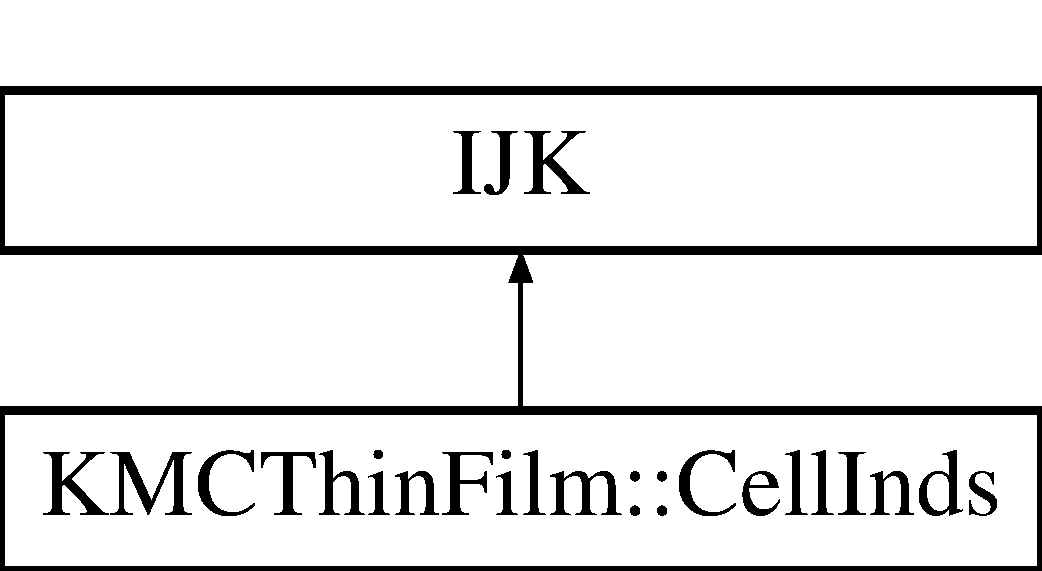
\includegraphics[height=2.000000cm]{classKMCThinFilm_1_1CellInds}
\end{center}
\end{figure}
\doxysubsubsection*{Public Member Functions}
\begin{DoxyCompactItemize}
\item 
\mbox{\hyperlink{classKMCThinFilm_1_1CellInds_a0534cf39ca2c6c8b35714eae3c97a151}{Cell\+Inds}} ()
\item 
\mbox{\hyperlink{classKMCThinFilm_1_1CellInds_a4c86adde21fec8a5ebcb3db217f0bca2}{Cell\+Inds}} (int ii, int jj, int kk=0)
\end{DoxyCompactItemize}


\doxysubsection{Detailed Description}
Indices of a lattice cell.

This class has three {\itshape public} data members, i, j, and k, which represent the first, second, and third indices. If the lattice has primitive lattice vectors ai, aj, and ak, then the location of the lattice cell may be taken as i\texorpdfstring{$\ast$}{*}ai + j\texorpdfstring{$\ast$}{*}aj + k\texorpdfstring{$\ast$}{*}ak.

\begin{DoxySeeAlso}{See also}
\doxylink{classKMCThinFilm_1_1CellIndsOffset}{Cell\+Inds\+Offset} \doxylink{namespaceKMCThinFilm_a57489af951d041dc66872aea47fa3da2}{KMCThin\+Film\+::operator+()} 
\end{DoxySeeAlso}
\begin{Desc}
\item[Examples]\par
\mbox{\hyperlink{testBallisticDep1_2EventsAndActions_8cpp-example}{test\+Ballistic\+Dep1/\+Events\+And\+Actions.\+cpp}}, \mbox{\hyperlink{testBallisticDep1_2EventsAndActions_8hpp-example}{test\+Ballistic\+Dep1/\+Events\+And\+Actions.\+hpp}}, \mbox{\hyperlink{testBallisticDep1_2InitLattice_8cpp-example}{test\+Ballistic\+Dep1/\+Init\+Lattice.\+cpp}}, \mbox{\hyperlink{testBallisticDep1_2InitLattice_8hpp-example}{test\+Ballistic\+Dep1/\+Init\+Lattice.\+hpp}}, \mbox{\hyperlink{testBallisticDep2_2EventsAndActions_8cpp-example}{test\+Ballistic\+Dep2/\+Events\+And\+Actions.\+cpp}}, \mbox{\hyperlink{testBallisticDep2_2EventsAndActions_8hpp-example}{test\+Ballistic\+Dep2/\+Events\+And\+Actions.\+hpp}}, \mbox{\hyperlink{testFractal_2EventsAndActions_8cpp-example}{test\+Fractal/\+Events\+And\+Actions.\+cpp}}, \mbox{\hyperlink{testFractal_2EventsAndActions_8hpp-example}{test\+Fractal/\+Events\+And\+Actions.\+hpp}}, \mbox{\hyperlink{testFractal_semi_manual_track_2EventsAndActions_8cpp-example}{test\+Fractal\+\_\+semi\+\_\+manual\+\_\+track/\+Events\+And\+Actions.\+cpp}}, \mbox{\hyperlink{testFractal_semi_manual_track_2EventsAndActions_8hpp-example}{test\+Fractal\+\_\+semi\+\_\+manual\+\_\+track/\+Events\+And\+Actions.\+hpp}}, \mbox{\hyperlink{testPatternedSurface1_2EventsAndActions_8cpp-example}{test\+Patterned\+Surface1/\+Events\+And\+Actions.\+cpp}}, \mbox{\hyperlink{testPatternedSurface1_2EventsAndActions_8hpp-example}{test\+Patterned\+Surface1/\+Events\+And\+Actions.\+hpp}}, \mbox{\hyperlink{testPatternedSurface1_2InitLattice_8cpp-example}{test\+Patterned\+Surface1/\+Init\+Lattice.\+cpp}}, \mbox{\hyperlink{testPatternedSurface2_2EventsAndActions_8cpp-example}{test\+Patterned\+Surface2/\+Events\+And\+Actions.\+cpp}}, and \mbox{\hyperlink{testPatternedSurface2_2EventsAndActions_8hpp-example}{test\+Patterned\+Surface2/\+Events\+And\+Actions.\+hpp}}.\end{Desc}


\doxysubsection{Constructor \& Destructor Documentation}
\Hypertarget{classKMCThinFilm_1_1CellInds_a0534cf39ca2c6c8b35714eae3c97a151}\index{KMCThinFilm::CellInds@{KMCThinFilm::CellInds}!CellInds@{CellInds}}
\index{CellInds@{CellInds}!KMCThinFilm::CellInds@{KMCThinFilm::CellInds}}
\doxysubsubsection{\texorpdfstring{CellInds()}{CellInds()}\hspace{0.1cm}{\footnotesize\ttfamily [1/2]}}
{\footnotesize\ttfamily \label{classKMCThinFilm_1_1CellInds_a0534cf39ca2c6c8b35714eae3c97a151} 
KMCThin\+Film\+::\+Cell\+Inds\+::\+Cell\+Inds (\begin{DoxyParamCaption}{}{}\end{DoxyParamCaption})\hspace{0.3cm}{\ttfamily [inline]}}

Constructs an empty \doxylink{classKMCThinFilm_1_1CellInds}{Cell\+Inds}. \Hypertarget{classKMCThinFilm_1_1CellInds_a4c86adde21fec8a5ebcb3db217f0bca2}\index{KMCThinFilm::CellInds@{KMCThinFilm::CellInds}!CellInds@{CellInds}}
\index{CellInds@{CellInds}!KMCThinFilm::CellInds@{KMCThinFilm::CellInds}}
\doxysubsubsection{\texorpdfstring{CellInds()}{CellInds()}\hspace{0.1cm}{\footnotesize\ttfamily [2/2]}}
{\footnotesize\ttfamily \label{classKMCThinFilm_1_1CellInds_a4c86adde21fec8a5ebcb3db217f0bca2} 
KMCThin\+Film\+::\+Cell\+Inds\+::\+Cell\+Inds (\begin{DoxyParamCaption}\item[{int}]{ii}{, }\item[{int}]{jj}{, }\item[{int}]{kk}{ = {\ttfamily 0}}\end{DoxyParamCaption})\hspace{0.3cm}{\ttfamily [inline]}}

Constructs a \doxylink{classKMCThinFilm_1_1CellInds}{Cell\+Inds} instance from a doublet or triplet of integers. 
\begin{DoxyParams}{Parameters}
{\em ii} & First index of a lattice cell  \\
\hline
{\em jj} & Second index of lattice cell  \\
\hline
{\em kk} & Third index of lattice cell \\
\hline
\end{DoxyParams}

\doxysection{KMCThin\+Film\+::Cell\+Inds\+Offset Class Reference}
\hypertarget{classKMCThinFilm_1_1CellIndsOffset}{}\label{classKMCThinFilm_1_1CellIndsOffset}\index{KMCThinFilm::CellIndsOffset@{KMCThinFilm::CellIndsOffset}}


{\ttfamily \#include $<$Cell\+Inds.\+hpp$>$}

Inheritance diagram for KMCThin\+Film\+::Cell\+Inds\+Offset\+:\begin{figure}[H]
\begin{center}
\leavevmode
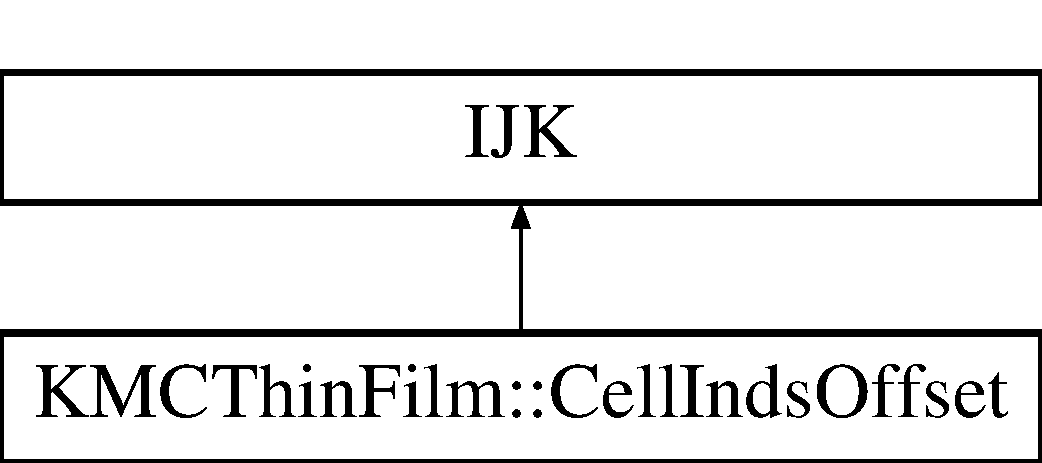
\includegraphics[height=2.000000cm]{classKMCThinFilm_1_1CellIndsOffset}
\end{center}
\end{figure}
\doxysubsubsection*{Public Member Functions}
\begin{DoxyCompactItemize}
\item 
\mbox{\hyperlink{classKMCThinFilm_1_1CellIndsOffset_af5409be7541eeb5c98f9ed771210b3cf}{Cell\+Inds\+Offset}} ()
\item 
\mbox{\hyperlink{classKMCThinFilm_1_1CellIndsOffset_a6d09182cb8481daba9d13a6815149258}{Cell\+Inds\+Offset}} (int ii, int jj, int kk=0)
\item 
\mbox{\hyperlink{classKMCThinFilm_1_1CellIndsOffset}{Cell\+Inds\+Offset}} \mbox{\hyperlink{classKMCThinFilm_1_1CellIndsOffset_abea5561250cff2e69fd7fbcd908b1f5c}{operator-\/}} () const
\end{DoxyCompactItemize}


\doxysubsection{Detailed Description}
An offset to indices of some lattice cell.

Like the \doxylink{classKMCThinFilm_1_1CellInds}{Cell\+Inds} class, it has three {\itshape public} data members, i, j, and k, which represent the offsets to be added to a given set of lattice cell indices. For example, one may write


\begin{DoxyCode}{0}
\DoxyCodeLine{CellInds\ ci(1,2,3);}
\DoxyCodeLine{CellInds\ offset(1,1,-\/1);}
\DoxyCodeLine{}
\DoxyCodeLine{CellInds\ ci\_w\_offset\ =\ ci\ +\ offset;}

\end{DoxyCode}


where the indices of ci\+\_\+w\+\_\+offset now equal 2, 3, and 2.

\begin{DoxySeeAlso}{See also}
\doxylink{classKMCThinFilm_1_1CellInds}{Cell\+Inds} \doxylink{namespaceKMCThinFilm_a57489af951d041dc66872aea47fa3da2}{KMCThin\+Film\+::operator+()} 
\end{DoxySeeAlso}
\begin{Desc}
\item[Examples]\par
\mbox{\hyperlink{testBallisticDep1_2EventsAndActions_8cpp-example}{test\+Ballistic\+Dep1/\+Events\+And\+Actions.\+cpp}}, \mbox{\hyperlink{testBallisticDep1_2testBallisticDep_8cpp-example}{test\+Ballistic\+Dep1/test\+Ballistic\+Dep.\+cpp}}, \mbox{\hyperlink{testBallisticDep2_2EventsAndActions_8cpp-example}{test\+Ballistic\+Dep2/\+Events\+And\+Actions.\+cpp}}, \mbox{\hyperlink{testBallisticDep2_2testBallisticDep_8cpp-example}{test\+Ballistic\+Dep2/test\+Ballistic\+Dep.\+cpp}}, \mbox{\hyperlink{testFractal_2testFractal_8cpp-example}{test\+Fractal/test\+Fractal.\+cpp}}, \mbox{\hyperlink{testFractal_parallel_2testFractal_8cpp-example}{test\+Fractal\+\_\+parallel/test\+Fractal.\+cpp}}, \mbox{\hyperlink{testFractal_semi_manual_track_2testFractal_8cpp-example}{test\+Fractal\+\_\+semi\+\_\+manual\+\_\+track/test\+Fractal.\+cpp}}, \mbox{\hyperlink{testPatternedSurface1_2testPatternedSurface_8cpp-example}{test\+Patterned\+Surface1/test\+Patterned\+Surface.\+cpp}}, and \mbox{\hyperlink{testPatternedSurface2_2testPatternedSurface_8cpp-example}{test\+Patterned\+Surface2/test\+Patterned\+Surface.\+cpp}}.\end{Desc}


\doxysubsection{Constructor \& Destructor Documentation}
\Hypertarget{classKMCThinFilm_1_1CellIndsOffset_af5409be7541eeb5c98f9ed771210b3cf}\index{KMCThinFilm::CellIndsOffset@{KMCThinFilm::CellIndsOffset}!CellIndsOffset@{CellIndsOffset}}
\index{CellIndsOffset@{CellIndsOffset}!KMCThinFilm::CellIndsOffset@{KMCThinFilm::CellIndsOffset}}
\doxysubsubsection{\texorpdfstring{CellIndsOffset()}{CellIndsOffset()}\hspace{0.1cm}{\footnotesize\ttfamily [1/2]}}
{\footnotesize\ttfamily \label{classKMCThinFilm_1_1CellIndsOffset_af5409be7541eeb5c98f9ed771210b3cf} 
KMCThin\+Film\+::\+Cell\+Inds\+Offset\+::\+Cell\+Inds\+Offset (\begin{DoxyParamCaption}{}{}\end{DoxyParamCaption})\hspace{0.3cm}{\ttfamily [inline]}}

Constructs an empty \doxylink{classKMCThinFilm_1_1CellIndsOffset}{Cell\+Inds\+Offset}. \Hypertarget{classKMCThinFilm_1_1CellIndsOffset_a6d09182cb8481daba9d13a6815149258}\index{KMCThinFilm::CellIndsOffset@{KMCThinFilm::CellIndsOffset}!CellIndsOffset@{CellIndsOffset}}
\index{CellIndsOffset@{CellIndsOffset}!KMCThinFilm::CellIndsOffset@{KMCThinFilm::CellIndsOffset}}
\doxysubsubsection{\texorpdfstring{CellIndsOffset()}{CellIndsOffset()}\hspace{0.1cm}{\footnotesize\ttfamily [2/2]}}
{\footnotesize\ttfamily \label{classKMCThinFilm_1_1CellIndsOffset_a6d09182cb8481daba9d13a6815149258} 
KMCThin\+Film\+::\+Cell\+Inds\+Offset\+::\+Cell\+Inds\+Offset (\begin{DoxyParamCaption}\item[{int}]{ii}{, }\item[{int}]{jj}{, }\item[{int}]{kk}{ = {\ttfamily 0}}\end{DoxyParamCaption})\hspace{0.3cm}{\ttfamily [inline]}}

Constructs a \doxylink{classKMCThinFilm_1_1CellIndsOffset}{Cell\+Inds\+Offset} instance from a doublet or triplet of integers. 
\begin{DoxyParams}{Parameters}
{\em ii} & Offset to the first index of a lattice cell  \\
\hline
{\em jj} & Offset to the second index of lattice cell  \\
\hline
{\em kk} & Offset to the third index of lattice cell \\
\hline
\end{DoxyParams}


\doxysubsection{Member Function Documentation}
\Hypertarget{classKMCThinFilm_1_1CellIndsOffset_abea5561250cff2e69fd7fbcd908b1f5c}\index{KMCThinFilm::CellIndsOffset@{KMCThinFilm::CellIndsOffset}!operator-\/@{operator-\/}}
\index{operator-\/@{operator-\/}!KMCThinFilm::CellIndsOffset@{KMCThinFilm::CellIndsOffset}}
\doxysubsubsection{\texorpdfstring{operator-\/()}{operator-()}}
{\footnotesize\ttfamily \label{classKMCThinFilm_1_1CellIndsOffset_abea5561250cff2e69fd7fbcd908b1f5c} 
\mbox{\hyperlink{classKMCThinFilm_1_1CellIndsOffset}{Cell\+Inds\+Offset}} KMCThin\+Film\+::\+Cell\+Inds\+Offset\+::operator-\/ (\begin{DoxyParamCaption}{}{}\end{DoxyParamCaption}) const}

Unary minus operator. Returns a sign-\/reversed copy of the offset. 
\doxysection{KMCThin\+Film\+::Cell\+Neigh\+Offsets Class Reference}
\hypertarget{classKMCThinFilm_1_1CellNeighOffsets}{}\label{classKMCThinFilm_1_1CellNeighOffsets}\index{KMCThinFilm::CellNeighOffsets@{KMCThinFilm::CellNeighOffsets}}


{\ttfamily \#include $<$Cell\+Neigh\+Offsets.\+hpp$>$}

\doxysubsubsection*{Public Member Functions}
\begin{DoxyCompactItemize}
\item 
\mbox{\hyperlink{classKMCThinFilm_1_1CellNeighOffsets_ae4b22e89dd2736a2d6e69c5efa88ad1e}{Cell\+Neigh\+Offsets}} (int number\+Of\+Offsets)
\item 
void \mbox{\hyperlink{classKMCThinFilm_1_1CellNeighOffsets_a7b983204101cef4973f685d3c68a0106}{add\+Offset}} (int which\+Offset, const \mbox{\hyperlink{classKMCThinFilm_1_1CellIndsOffset}{Cell\+Inds\+Offset}} \&offset)
\item 
void \mbox{\hyperlink{classKMCThinFilm_1_1CellNeighOffsets_aded2dfb4016a51aac9f7fe1b114fc261}{clear\+Offsets}} ()
\item 
const \mbox{\hyperlink{classKMCThinFilm_1_1CellIndsOffset}{Cell\+Inds\+Offset}} \& \mbox{\hyperlink{classKMCThinFilm_1_1CellNeighOffsets_acf082422c1ab26aa5144d98426f34ab2}{get\+Offset}} (int which\+Offset) const
\item 
int \mbox{\hyperlink{classKMCThinFilm_1_1CellNeighOffsets_a946a91c1759eb1dec7509984f4cdab03}{num\+Offsets}} () const
\item 
void \mbox{\hyperlink{classKMCThinFilm_1_1CellNeighOffsets_ac0ff865663588ae531dd6b4251eca368}{reset\+Offsets}} (int number\+Of\+New\+Offsets)
\end{DoxyCompactItemize}


\doxysubsection{Detailed Description}
Collection of \doxylink{classKMCThinFilm_1_1CellIndsOffset}{Cell\+Inds\+Offset} objects that are used to determine an event\textquotesingle{}s propensity.

Each offset in the collection is associated with an integer ID. No matter what, this collection always contains a \doxylink{classKMCThinFilm_1_1CellIndsOffset}{Cell\+Inds\+Offset} object with the indices (0,0,0), and this offset has the integer ID of zero. \begin{Desc}
\item[Examples]\par
\mbox{\hyperlink{testBallisticDep1_2EventsAndActions_8cpp-example}{test\+Ballistic\+Dep1/\+Events\+And\+Actions.\+cpp}}, \mbox{\hyperlink{testBallisticDep1_2testBallisticDep_8cpp-example}{test\+Ballistic\+Dep1/test\+Ballistic\+Dep.\+cpp}}, \mbox{\hyperlink{testBallisticDep2_2EventsAndActions_8cpp-example}{test\+Ballistic\+Dep2/\+Events\+And\+Actions.\+cpp}}, \mbox{\hyperlink{testBallisticDep2_2testBallisticDep_8cpp-example}{test\+Ballistic\+Dep2/test\+Ballistic\+Dep.\+cpp}}, \mbox{\hyperlink{testFractal_2testFractal_8cpp-example}{test\+Fractal/test\+Fractal.\+cpp}}, \mbox{\hyperlink{testFractal_parallel_2testFractal_8cpp-example}{test\+Fractal\+\_\+parallel/test\+Fractal.\+cpp}}, \mbox{\hyperlink{testFractal_semi_manual_track_2testFractal_8cpp-example}{test\+Fractal\+\_\+semi\+\_\+manual\+\_\+track/test\+Fractal.\+cpp}}, \mbox{\hyperlink{testPatternedSurface1_2testPatternedSurface_8cpp-example}{test\+Patterned\+Surface1/test\+Patterned\+Surface.\+cpp}}, and \mbox{\hyperlink{testPatternedSurface2_2testPatternedSurface_8cpp-example}{test\+Patterned\+Surface2/test\+Patterned\+Surface.\+cpp}}.\end{Desc}


\doxysubsection{Constructor \& Destructor Documentation}
\Hypertarget{classKMCThinFilm_1_1CellNeighOffsets_ae4b22e89dd2736a2d6e69c5efa88ad1e}\index{KMCThinFilm::CellNeighOffsets@{KMCThinFilm::CellNeighOffsets}!CellNeighOffsets@{CellNeighOffsets}}
\index{CellNeighOffsets@{CellNeighOffsets}!KMCThinFilm::CellNeighOffsets@{KMCThinFilm::CellNeighOffsets}}
\doxysubsubsection{\texorpdfstring{CellNeighOffsets()}{CellNeighOffsets()}}
{\footnotesize\ttfamily \label{classKMCThinFilm_1_1CellNeighOffsets_ae4b22e89dd2736a2d6e69c5efa88ad1e} 
KMCThin\+Film\+::\+Cell\+Neigh\+Offsets\+::\+Cell\+Neigh\+Offsets (\begin{DoxyParamCaption}\item[{int}]{number\+Of\+Offsets}{}\end{DoxyParamCaption})\hspace{0.3cm}{\ttfamily [explicit]}}

Constructs a \doxylink{classKMCThinFilm_1_1CellNeighOffsets}{Cell\+Neigh\+Offsets} object. 
\begin{DoxyParams}{Parameters}
{\em number\+Of\+Offsets} & Number of offsets to be added. \\
\hline
\end{DoxyParams}


\doxysubsection{Member Function Documentation}
\Hypertarget{classKMCThinFilm_1_1CellNeighOffsets_a7b983204101cef4973f685d3c68a0106}\index{KMCThinFilm::CellNeighOffsets@{KMCThinFilm::CellNeighOffsets}!addOffset@{addOffset}}
\index{addOffset@{addOffset}!KMCThinFilm::CellNeighOffsets@{KMCThinFilm::CellNeighOffsets}}
\doxysubsubsection{\texorpdfstring{addOffset()}{addOffset()}}
{\footnotesize\ttfamily \label{classKMCThinFilm_1_1CellNeighOffsets_a7b983204101cef4973f685d3c68a0106} 
void KMCThin\+Film\+::\+Cell\+Neigh\+Offsets\+::add\+Offset (\begin{DoxyParamCaption}\item[{int}]{which\+Offset}{, }\item[{const \mbox{\hyperlink{classKMCThinFilm_1_1CellIndsOffset}{Cell\+Inds\+Offset}} \&}]{offset}{}\end{DoxyParamCaption})}

Adds an additional offset.

The argument {\itshape which\+Offset} is not allowed to be zero, since that integer ID is already associated with the offset (0,0,0). 
\begin{DoxyParams}{Parameters}
{\em which\+Offset} & Integer ID of offset. Must be \texorpdfstring{$>$}{>}= 1 and less than \doxylink{classKMCThinFilm_1_1CellNeighOffsets_a946a91c1759eb1dec7509984f4cdab03}{num\+Offsets()}  \\
\hline
{\em offset} & The offset to be added. \\
\hline
\end{DoxyParams}
\begin{Desc}
\item[Examples]\par
\mbox{\hyperlink{testBallisticDep1_2testBallisticDep_8cpp-example}{test\+Ballistic\+Dep1/test\+Ballistic\+Dep.\+cpp}}, \mbox{\hyperlink{testBallisticDep2_2testBallisticDep_8cpp-example}{test\+Ballistic\+Dep2/test\+Ballistic\+Dep.\+cpp}}, \mbox{\hyperlink{testFractal_2testFractal_8cpp-example}{test\+Fractal/test\+Fractal.\+cpp}}, \mbox{\hyperlink{testFractal_parallel_2testFractal_8cpp-example}{test\+Fractal\+\_\+parallel/test\+Fractal.\+cpp}}, \mbox{\hyperlink{testFractal_semi_manual_track_2testFractal_8cpp-example}{test\+Fractal\+\_\+semi\+\_\+manual\+\_\+track/test\+Fractal.\+cpp}}, \mbox{\hyperlink{testPatternedSurface1_2testPatternedSurface_8cpp-example}{test\+Patterned\+Surface1/test\+Patterned\+Surface.\+cpp}}, and \mbox{\hyperlink{testPatternedSurface2_2testPatternedSurface_8cpp-example}{test\+Patterned\+Surface2/test\+Patterned\+Surface.\+cpp}}.\end{Desc}
\Hypertarget{classKMCThinFilm_1_1CellNeighOffsets_aded2dfb4016a51aac9f7fe1b114fc261}\index{KMCThinFilm::CellNeighOffsets@{KMCThinFilm::CellNeighOffsets}!clearOffsets@{clearOffsets}}
\index{clearOffsets@{clearOffsets}!KMCThinFilm::CellNeighOffsets@{KMCThinFilm::CellNeighOffsets}}
\doxysubsubsection{\texorpdfstring{clearOffsets()}{clearOffsets()}}
{\footnotesize\ttfamily \label{classKMCThinFilm_1_1CellNeighOffsets_aded2dfb4016a51aac9f7fe1b114fc261} 
void KMCThin\+Film\+::\+Cell\+Neigh\+Offsets\+::clear\+Offsets (\begin{DoxyParamCaption}{}{}\end{DoxyParamCaption})}

Removes all previously added offsets.

Note that no new offsets may be added until \doxylink{classKMCThinFilm_1_1CellNeighOffsets_ac0ff865663588ae531dd6b4251eca368}{reset\+Offsets()} is called. \Hypertarget{classKMCThinFilm_1_1CellNeighOffsets_acf082422c1ab26aa5144d98426f34ab2}\index{KMCThinFilm::CellNeighOffsets@{KMCThinFilm::CellNeighOffsets}!getOffset@{getOffset}}
\index{getOffset@{getOffset}!KMCThinFilm::CellNeighOffsets@{KMCThinFilm::CellNeighOffsets}}
\doxysubsubsection{\texorpdfstring{getOffset()}{getOffset()}}
{\footnotesize\ttfamily \label{classKMCThinFilm_1_1CellNeighOffsets_acf082422c1ab26aa5144d98426f34ab2} 
const \mbox{\hyperlink{classKMCThinFilm_1_1CellIndsOffset}{Cell\+Inds\+Offset}} \& KMCThin\+Film\+::\+Cell\+Neigh\+Offsets\+::get\+Offset (\begin{DoxyParamCaption}\item[{int}]{which\+Offset}{}\end{DoxyParamCaption}) const}

Returns the offset with the integer ID {\itshape which\+Offset}. Note that, here, {\itshape which\+Offset} {\itshape is} allowed to be zero. 
\begin{DoxyParams}{Parameters}
{\em which\+Offset} & Integer ID of offset. \\
\hline
\end{DoxyParams}
\begin{Desc}
\item[Examples]\par
\mbox{\hyperlink{testFractal_parallel_2testFractal_8cpp-example}{test\+Fractal\+\_\+parallel/test\+Fractal.\+cpp}}, \mbox{\hyperlink{testFractal_semi_manual_track_2testFractal_8cpp-example}{test\+Fractal\+\_\+semi\+\_\+manual\+\_\+track/test\+Fractal.\+cpp}}, \mbox{\hyperlink{testPatternedSurface1_2testPatternedSurface_8cpp-example}{test\+Patterned\+Surface1/test\+Patterned\+Surface.\+cpp}}, and \mbox{\hyperlink{testPatternedSurface2_2testPatternedSurface_8cpp-example}{test\+Patterned\+Surface2/test\+Patterned\+Surface.\+cpp}}.\end{Desc}
\Hypertarget{classKMCThinFilm_1_1CellNeighOffsets_a946a91c1759eb1dec7509984f4cdab03}\index{KMCThinFilm::CellNeighOffsets@{KMCThinFilm::CellNeighOffsets}!numOffsets@{numOffsets}}
\index{numOffsets@{numOffsets}!KMCThinFilm::CellNeighOffsets@{KMCThinFilm::CellNeighOffsets}}
\doxysubsubsection{\texorpdfstring{numOffsets()}{numOffsets()}}
{\footnotesize\ttfamily \label{classKMCThinFilm_1_1CellNeighOffsets_a946a91c1759eb1dec7509984f4cdab03} 
int KMCThin\+Film\+::\+Cell\+Neigh\+Offsets\+::num\+Offsets (\begin{DoxyParamCaption}{}{}\end{DoxyParamCaption}) const}

Number of offsets stored. \Hypertarget{classKMCThinFilm_1_1CellNeighOffsets_ac0ff865663588ae531dd6b4251eca368}\index{KMCThinFilm::CellNeighOffsets@{KMCThinFilm::CellNeighOffsets}!resetOffsets@{resetOffsets}}
\index{resetOffsets@{resetOffsets}!KMCThinFilm::CellNeighOffsets@{KMCThinFilm::CellNeighOffsets}}
\doxysubsubsection{\texorpdfstring{resetOffsets()}{resetOffsets()}}
{\footnotesize\ttfamily \label{classKMCThinFilm_1_1CellNeighOffsets_ac0ff865663588ae531dd6b4251eca368} 
void KMCThin\+Film\+::\+Cell\+Neigh\+Offsets\+::reset\+Offsets (\begin{DoxyParamCaption}\item[{int}]{number\+Of\+New\+Offsets}{}\end{DoxyParamCaption})}

Removes all previous offsets and allocates memory for {\itshape number\+Of\+New\+Offsets} \doxylink{classKMCThinFilm_1_1CellIndsOffset}{Cell\+Inds\+Offset} objects. 
\doxysection{KMCThin\+Film\+::Cell\+Neigh\+Probe Class Reference}
\hypertarget{classKMCThinFilm_1_1CellNeighProbe}{}\label{classKMCThinFilm_1_1CellNeighProbe}\index{KMCThinFilm::CellNeighProbe@{KMCThinFilm::CellNeighProbe}}


{\ttfamily \#include $<$Cell\+Neigh\+Probe.\+hpp$>$}

\doxysubsubsection*{Public Member Functions}
\begin{DoxyCompactItemize}
\item 
\mbox{\hyperlink{classKMCThinFilm_1_1CellNeighProbe_a4388328e433e84f9407d0ca7e85b4db2}{Cell\+Neigh\+Probe}} (const \mbox{\hyperlink{classKMCThinFilm_1_1Lattice}{Lattice}} \texorpdfstring{$\ast$}{*}lattice=NULL)
\item 
void \mbox{\hyperlink{classKMCThinFilm_1_1CellNeighProbe_a02d5bd2dd43aa7b17a6fcc7efe345443}{attach\+Cell\+Inds}} (const \mbox{\hyperlink{classKMCThinFilm_1_1CellInds}{Cell\+Inds}} \texorpdfstring{$\ast$}{*}ci, const std\+::vector$<$ \mbox{\hyperlink{classKMCThinFilm_1_1CellIndsOffset}{Cell\+Inds\+Offset}} $>$ \texorpdfstring{$\ast$}{*}cio\+Vec\+Ptr)
\item 
void \mbox{\hyperlink{classKMCThinFilm_1_1CellNeighProbe_ace997a38840ebc55993f6a98645b7808}{attach\+Lattice}} (const \mbox{\hyperlink{classKMCThinFilm_1_1Lattice}{Lattice}} \texorpdfstring{$\ast$}{*}lattice)
\item 
bool \mbox{\hyperlink{classKMCThinFilm_1_1CellNeighProbe_acff2debf7ca2157b8ea1d58475a9f25f}{below\+Lattice\+Bottom}} (const \mbox{\hyperlink{classKMCThinFilm_1_1CellToProbe}{Cell\+To\+Probe}} \&ctp) const
\item 
bool \mbox{\hyperlink{classKMCThinFilm_1_1CellNeighProbe_a1c68a11a6d1af530abf21ed070ae452c}{exceeds\+Lattice\+Height}} (const \mbox{\hyperlink{classKMCThinFilm_1_1CellToProbe}{Cell\+To\+Probe}} \&ctp) const
\item 
\mbox{\hyperlink{classKMCThinFilm_1_1CellToProbe}{Cell\+To\+Probe}} \mbox{\hyperlink{classKMCThinFilm_1_1CellNeighProbe_a1ba997186f6326b525dd66df4254d198}{get\+Cell\+To\+Probe}} (int probed\+Cell\+Ind) const
\item 
double \mbox{\hyperlink{classKMCThinFilm_1_1CellNeighProbe_a1425c18df394e394b7c50e9f332371fc}{get\+Float}} (const \mbox{\hyperlink{classKMCThinFilm_1_1CellToProbe}{Cell\+To\+Probe}} \&ctp, int which\+Float) const
\item 
int \mbox{\hyperlink{classKMCThinFilm_1_1CellNeighProbe_a7be3ba45264054167a243f15a1954b92}{get\+Int}} (const \mbox{\hyperlink{classKMCThinFilm_1_1CellToProbe}{Cell\+To\+Probe}} \&ctp, int which\+Int) const
\end{DoxyCompactItemize}


\doxysubsection{Detailed Description}
A class used by a Cell\+Centered\+Propensity function object to probe the states of neighboring lattice cells in order to determine a cell-\/centered event\textquotesingle{}s propensity.

Each neighboring lattice cell is identified by one of the integer IDs used to label the offsets inside a \doxylink{classKMCThinFilm_1_1CellNeighOffsets}{Cell\+Neigh\+Offsets} object, and the indices of this neighboring lattice cell are that of the current cell (about which an event is centered) plus the offset corresponding to its integer ID. \begin{Desc}
\item[Examples]\par
\mbox{\hyperlink{testBallisticDep1_2EventsAndActions_8cpp-example}{test\+Ballistic\+Dep1/\+Events\+And\+Actions.\+cpp}}, \mbox{\hyperlink{testBallisticDep2_2EventsAndActions_8cpp-example}{test\+Ballistic\+Dep2/\+Events\+And\+Actions.\+cpp}}, \mbox{\hyperlink{testFractal_2EventsAndActions_8cpp-example}{test\+Fractal/\+Events\+And\+Actions.\+cpp}}, \mbox{\hyperlink{testFractal_2EventsAndActions_8hpp-example}{test\+Fractal/\+Events\+And\+Actions.\+hpp}}, \mbox{\hyperlink{testFractal_semi_manual_track_2EventsAndActions_8cpp-example}{test\+Fractal\+\_\+semi\+\_\+manual\+\_\+track/\+Events\+And\+Actions.\+cpp}}, \mbox{\hyperlink{testFractal_semi_manual_track_2EventsAndActions_8hpp-example}{test\+Fractal\+\_\+semi\+\_\+manual\+\_\+track/\+Events\+And\+Actions.\+hpp}}, \mbox{\hyperlink{testPatternedSurface1_2EventsAndActions_8cpp-example}{test\+Patterned\+Surface1/\+Events\+And\+Actions.\+cpp}}, \mbox{\hyperlink{testPatternedSurface1_2EventsAndActions_8hpp-example}{test\+Patterned\+Surface1/\+Events\+And\+Actions.\+hpp}}, \mbox{\hyperlink{testPatternedSurface2_2EventsAndActions_8cpp-example}{test\+Patterned\+Surface2/\+Events\+And\+Actions.\+cpp}}, and \mbox{\hyperlink{testPatternedSurface2_2EventsAndActions_8hpp-example}{test\+Patterned\+Surface2/\+Events\+And\+Actions.\+hpp}}.\end{Desc}


\doxysubsection{Constructor \& Destructor Documentation}
\Hypertarget{classKMCThinFilm_1_1CellNeighProbe_a4388328e433e84f9407d0ca7e85b4db2}\index{KMCThinFilm::CellNeighProbe@{KMCThinFilm::CellNeighProbe}!CellNeighProbe@{CellNeighProbe}}
\index{CellNeighProbe@{CellNeighProbe}!KMCThinFilm::CellNeighProbe@{KMCThinFilm::CellNeighProbe}}
\doxysubsubsection{\texorpdfstring{CellNeighProbe()}{CellNeighProbe()}}
{\footnotesize\ttfamily \label{classKMCThinFilm_1_1CellNeighProbe_a4388328e433e84f9407d0ca7e85b4db2} 
KMCThin\+Film\+::\+Cell\+Neigh\+Probe\+::\+Cell\+Neigh\+Probe (\begin{DoxyParamCaption}\item[{const \mbox{\hyperlink{classKMCThinFilm_1_1Lattice}{Lattice}} \texorpdfstring{$\ast$}{*}}]{lattice}{ = {\ttfamily NULL}}\end{DoxyParamCaption})\hspace{0.3cm}{\ttfamily [explicit]}}

\mbox{[}{\bfseries{ADVANCED}}\mbox{]} Constructs a \doxylink{classKMCThinFilm_1_1CellNeighProbe}{Cell\+Neigh\+Probe} and attaches it to a \doxylink{classKMCThinFilm_1_1Lattice}{Lattice} object. Mainly for use in testing and debugging. 

\doxysubsection{Member Function Documentation}
\Hypertarget{classKMCThinFilm_1_1CellNeighProbe_a02d5bd2dd43aa7b17a6fcc7efe345443}\index{KMCThinFilm::CellNeighProbe@{KMCThinFilm::CellNeighProbe}!attachCellInds@{attachCellInds}}
\index{attachCellInds@{attachCellInds}!KMCThinFilm::CellNeighProbe@{KMCThinFilm::CellNeighProbe}}
\doxysubsubsection{\texorpdfstring{attachCellInds()}{attachCellInds()}}
{\footnotesize\ttfamily \label{classKMCThinFilm_1_1CellNeighProbe_a02d5bd2dd43aa7b17a6fcc7efe345443} 
void KMCThin\+Film\+::\+Cell\+Neigh\+Probe\+::attach\+Cell\+Inds (\begin{DoxyParamCaption}\item[{const \mbox{\hyperlink{classKMCThinFilm_1_1CellInds}{Cell\+Inds}} \texorpdfstring{$\ast$}{*}}]{ci}{, }\item[{const std\+::vector$<$ \mbox{\hyperlink{classKMCThinFilm_1_1CellIndsOffset}{Cell\+Inds\+Offset}} $>$ \texorpdfstring{$\ast$}{*}}]{cio\+Vec\+Ptr}{}\end{DoxyParamCaption})}

\mbox{[}{\bfseries{ADVANCED}}\mbox{]} Attaches a vector of \doxylink{classKMCThinFilm_1_1CellIndsOffset}{Cell\+Inds\+Offset} objects (generated from a \doxylink{classKMCThinFilm_1_1CellNeighOffsets}{Cell\+Neigh\+Offsets} instance). Mainly for use in testing and debugging. 
\begin{DoxyParams}{Parameters}
{\em ci} & Pointer to the indices of the cell about which an event is centered.  \\
\hline
{\em cio\+Vec\+Ptr} & Pointer to the vector of \doxylink{classKMCThinFilm_1_1CellIndsOffset}{Cell\+Inds\+Offset} objects that define the neighboring lattice cells used to calculate the propensity of the event. \\
\hline
\end{DoxyParams}
\Hypertarget{classKMCThinFilm_1_1CellNeighProbe_ace997a38840ebc55993f6a98645b7808}\index{KMCThinFilm::CellNeighProbe@{KMCThinFilm::CellNeighProbe}!attachLattice@{attachLattice}}
\index{attachLattice@{attachLattice}!KMCThinFilm::CellNeighProbe@{KMCThinFilm::CellNeighProbe}}
\doxysubsubsection{\texorpdfstring{attachLattice()}{attachLattice()}}
{\footnotesize\ttfamily \label{classKMCThinFilm_1_1CellNeighProbe_ace997a38840ebc55993f6a98645b7808} 
void KMCThin\+Film\+::\+Cell\+Neigh\+Probe\+::attach\+Lattice (\begin{DoxyParamCaption}\item[{const \mbox{\hyperlink{classKMCThinFilm_1_1Lattice}{Lattice}} \texorpdfstring{$\ast$}{*}}]{lattice}{}\end{DoxyParamCaption})}

\mbox{[}{\bfseries{ADVANCED}}\mbox{]} Attaches a \doxylink{classKMCThinFilm_1_1Lattice}{Lattice} object, replacing whatever lattice object that was attached before. Mainly for use in testing and debugging. \Hypertarget{classKMCThinFilm_1_1CellNeighProbe_acff2debf7ca2157b8ea1d58475a9f25f}\index{KMCThinFilm::CellNeighProbe@{KMCThinFilm::CellNeighProbe}!belowLatticeBottom@{belowLatticeBottom}}
\index{belowLatticeBottom@{belowLatticeBottom}!KMCThinFilm::CellNeighProbe@{KMCThinFilm::CellNeighProbe}}
\doxysubsubsection{\texorpdfstring{belowLatticeBottom()}{belowLatticeBottom()}}
{\footnotesize\ttfamily \label{classKMCThinFilm_1_1CellNeighProbe_acff2debf7ca2157b8ea1d58475a9f25f} 
bool KMCThin\+Film\+::\+Cell\+Neigh\+Probe\+::below\+Lattice\+Bottom (\begin{DoxyParamCaption}\item[{const \mbox{\hyperlink{classKMCThinFilm_1_1CellToProbe}{Cell\+To\+Probe}} \&}]{ctp}{}\end{DoxyParamCaption}) const}

Indicates whether the height coordinate of the (possibly non-\/existent) lattice cell pointed to by {\itshape ctp} is less than zero. If true, it implies that this lattice cell does not and will not actually exist in the simulation. \begin{Desc}
\item[Examples]\par
\mbox{\hyperlink{testBallisticDep1_2EventsAndActions_8cpp-example}{test\+Ballistic\+Dep1/\+Events\+And\+Actions.\+cpp}}, and \mbox{\hyperlink{testBallisticDep2_2EventsAndActions_8cpp-example}{test\+Ballistic\+Dep2/\+Events\+And\+Actions.\+cpp}}.\end{Desc}
\Hypertarget{classKMCThinFilm_1_1CellNeighProbe_a1c68a11a6d1af530abf21ed070ae452c}\index{KMCThinFilm::CellNeighProbe@{KMCThinFilm::CellNeighProbe}!exceedsLatticeHeight@{exceedsLatticeHeight}}
\index{exceedsLatticeHeight@{exceedsLatticeHeight}!KMCThinFilm::CellNeighProbe@{KMCThinFilm::CellNeighProbe}}
\doxysubsubsection{\texorpdfstring{exceedsLatticeHeight()}{exceedsLatticeHeight()}}
{\footnotesize\ttfamily \label{classKMCThinFilm_1_1CellNeighProbe_a1c68a11a6d1af530abf21ed070ae452c} 
bool KMCThin\+Film\+::\+Cell\+Neigh\+Probe\+::exceeds\+Lattice\+Height (\begin{DoxyParamCaption}\item[{const \mbox{\hyperlink{classKMCThinFilm_1_1CellToProbe}{Cell\+To\+Probe}} \&}]{ctp}{}\end{DoxyParamCaption}) const}

Indicates whether the height coordinate of the (possibly non-\/existent) lattice cell pointed to by {\itshape ctp} exceeds the current height of the lattice. If true, it implies that this lattice cell does not actually exist yet in the simulation. \begin{Desc}
\item[Examples]\par
\mbox{\hyperlink{testBallisticDep1_2EventsAndActions_8cpp-example}{test\+Ballistic\+Dep1/\+Events\+And\+Actions.\+cpp}}, and \mbox{\hyperlink{testBallisticDep2_2EventsAndActions_8cpp-example}{test\+Ballistic\+Dep2/\+Events\+And\+Actions.\+cpp}}.\end{Desc}
\Hypertarget{classKMCThinFilm_1_1CellNeighProbe_a1ba997186f6326b525dd66df4254d198}\index{KMCThinFilm::CellNeighProbe@{KMCThinFilm::CellNeighProbe}!getCellToProbe@{getCellToProbe}}
\index{getCellToProbe@{getCellToProbe}!KMCThinFilm::CellNeighProbe@{KMCThinFilm::CellNeighProbe}}
\doxysubsubsection{\texorpdfstring{getCellToProbe()}{getCellToProbe()}}
{\footnotesize\ttfamily \label{classKMCThinFilm_1_1CellNeighProbe_a1ba997186f6326b525dd66df4254d198} 
\mbox{\hyperlink{classKMCThinFilm_1_1CellToProbe}{Cell\+To\+Probe}} KMCThin\+Film\+::\+Cell\+Neigh\+Probe\+::get\+Cell\+To\+Probe (\begin{DoxyParamCaption}\item[{int}]{probed\+Cell\+Ind}{}\end{DoxyParamCaption}) const}

Retrieves the lattice cell to be probed from its integer ID. 
\begin{DoxyParams}{Parameters}
{\em probed\+Cell\+Ind} & Integer ID of the lattice cell (and its corresponding offset). \\
\hline
\end{DoxyParams}
\begin{Desc}
\item[Examples]\par
\mbox{\hyperlink{testBallisticDep1_2EventsAndActions_8cpp-example}{test\+Ballistic\+Dep1/\+Events\+And\+Actions.\+cpp}}, \mbox{\hyperlink{testBallisticDep2_2EventsAndActions_8cpp-example}{test\+Ballistic\+Dep2/\+Events\+And\+Actions.\+cpp}}, \mbox{\hyperlink{testFractal_2EventsAndActions_8cpp-example}{test\+Fractal/\+Events\+And\+Actions.\+cpp}}, \mbox{\hyperlink{testFractal_semi_manual_track_2EventsAndActions_8cpp-example}{test\+Fractal\+\_\+semi\+\_\+manual\+\_\+track/\+Events\+And\+Actions.\+cpp}}, \mbox{\hyperlink{testPatternedSurface1_2EventsAndActions_8cpp-example}{test\+Patterned\+Surface1/\+Events\+And\+Actions.\+cpp}}, and \mbox{\hyperlink{testPatternedSurface2_2EventsAndActions_8cpp-example}{test\+Patterned\+Surface2/\+Events\+And\+Actions.\+cpp}}.\end{Desc}
\Hypertarget{classKMCThinFilm_1_1CellNeighProbe_a1425c18df394e394b7c50e9f332371fc}\index{KMCThinFilm::CellNeighProbe@{KMCThinFilm::CellNeighProbe}!getFloat@{getFloat}}
\index{getFloat@{getFloat}!KMCThinFilm::CellNeighProbe@{KMCThinFilm::CellNeighProbe}}
\doxysubsubsection{\texorpdfstring{getFloat()}{getFloat()}}
{\footnotesize\ttfamily \label{classKMCThinFilm_1_1CellNeighProbe_a1425c18df394e394b7c50e9f332371fc} 
double KMCThin\+Film\+::\+Cell\+Neigh\+Probe\+::get\+Float (\begin{DoxyParamCaption}\item[{const \mbox{\hyperlink{classKMCThinFilm_1_1CellToProbe}{Cell\+To\+Probe}} \&}]{ctp}{, }\item[{int}]{which\+Float}{}\end{DoxyParamCaption}) const}

Retrieves one of the floating-\/point values (if present) from the lattice cell pointed to by {\itshape ctp}. The parameter {\itshape which\+Float} indicates which of the floating-\/point values to return. \begin{Desc}
\item[Examples]\par
\mbox{\hyperlink{testPatternedSurface1_2EventsAndActions_8cpp-example}{test\+Patterned\+Surface1/\+Events\+And\+Actions.\+cpp}}.\end{Desc}
\Hypertarget{classKMCThinFilm_1_1CellNeighProbe_a7be3ba45264054167a243f15a1954b92}\index{KMCThinFilm::CellNeighProbe@{KMCThinFilm::CellNeighProbe}!getInt@{getInt}}
\index{getInt@{getInt}!KMCThinFilm::CellNeighProbe@{KMCThinFilm::CellNeighProbe}}
\doxysubsubsection{\texorpdfstring{getInt()}{getInt()}}
{\footnotesize\ttfamily \label{classKMCThinFilm_1_1CellNeighProbe_a7be3ba45264054167a243f15a1954b92} 
int KMCThin\+Film\+::\+Cell\+Neigh\+Probe\+::get\+Int (\begin{DoxyParamCaption}\item[{const \mbox{\hyperlink{classKMCThinFilm_1_1CellToProbe}{Cell\+To\+Probe}} \&}]{ctp}{, }\item[{int}]{which\+Int}{}\end{DoxyParamCaption}) const}

Retrieves one of the integer values (if present) from the lattice cell pointed to by {\itshape ctp}. The parameter {\itshape which\+Int} indicates which of the integer values to return. \begin{Desc}
\item[Examples]\par
\mbox{\hyperlink{testBallisticDep1_2EventsAndActions_8cpp-example}{test\+Ballistic\+Dep1/\+Events\+And\+Actions.\+cpp}}, \mbox{\hyperlink{testBallisticDep2_2EventsAndActions_8cpp-example}{test\+Ballistic\+Dep2/\+Events\+And\+Actions.\+cpp}}, \mbox{\hyperlink{testFractal_2EventsAndActions_8cpp-example}{test\+Fractal/\+Events\+And\+Actions.\+cpp}}, \mbox{\hyperlink{testFractal_semi_manual_track_2EventsAndActions_8cpp-example}{test\+Fractal\+\_\+semi\+\_\+manual\+\_\+track/\+Events\+And\+Actions.\+cpp}}, \mbox{\hyperlink{testPatternedSurface1_2EventsAndActions_8cpp-example}{test\+Patterned\+Surface1/\+Events\+And\+Actions.\+cpp}}, and \mbox{\hyperlink{testPatternedSurface2_2EventsAndActions_8cpp-example}{test\+Patterned\+Surface2/\+Events\+And\+Actions.\+cpp}}.\end{Desc}

\doxysection{KMCThin\+Film\+::Cells\+To\+Change Class Reference}
\hypertarget{classKMCThinFilm_1_1CellsToChange}{}\label{classKMCThinFilm_1_1CellsToChange}\index{KMCThinFilm::CellsToChange@{KMCThinFilm::CellsToChange}}


{\ttfamily \#include $<$Cells\+To\+Change.\+hpp$>$}

\doxysubsubsection*{Public Member Functions}
\begin{DoxyCompactItemize}
\item 
void \mbox{\hyperlink{classKMCThinFilm_1_1CellsToChange_a6753306ace3d33af03814bfb048498b5}{add\+Lattice\+Planes}} (int num\+Planes\+To\+Add)
\item 
const \mbox{\hyperlink{classKMCThinFilm_1_1CellInds}{Cell\+Inds}} \& \mbox{\hyperlink{classKMCThinFilm_1_1CellsToChange_ae76e3b5b096b7aa6988f059a7c2c78a4}{get\+Cell\+Inds}} (int which\+Offset) const
\item 
double \mbox{\hyperlink{classKMCThinFilm_1_1CellsToChange_a072e22624e2eafdb9dc8fd0067f763b5}{get\+Float}} (int which\+Offset, int which\+Float) const
\item 
int \mbox{\hyperlink{classKMCThinFilm_1_1CellsToChange_ae559a33ad8206a5e1c8cfd8803ccc765}{get\+Int}} (int which\+Offset, int which\+Int) const
\item 
void \mbox{\hyperlink{classKMCThinFilm_1_1CellsToChange_a8a56c1106701d5bc3409cd30343fee2c}{set\+Center}} (const \mbox{\hyperlink{classKMCThinFilm_1_1CellInds}{Cell\+Inds}} \&ci)
\item 
void \mbox{\hyperlink{classKMCThinFilm_1_1CellsToChange_a0e89c1262df5b89f00329e685a9871fa}{set\+Float}} (int which\+Offset, int which\+Float, double val)
\item 
void \mbox{\hyperlink{classKMCThinFilm_1_1CellsToChange_a62079b840cc200e37e2907ba2e394f78}{set\+Int}} (int which\+Offset, int which\+Int, int val)
\end{DoxyCompactItemize}
\doxysubsubsection*{Friends}
\begin{DoxyCompactItemize}
\item 
\Hypertarget{classKMCThinFilm_1_1CellsToChange_aeb51e0a4c44d4192cfbdb79598859172}\label{classKMCThinFilm_1_1CellsToChange_aeb51e0a4c44d4192cfbdb79598859172} 
class {\bfseries Simulation}
\end{DoxyCompactItemize}


\doxysubsection{Detailed Description}
Class used to change the lattice when using a function object satisfying the \doxylink{namespaceKMCThinFilm_a92a9e6c3ced8703f95265e85d80f1797}{Event\+Executor\+Semi\+Manual\+Track} signature to execute an event.

Instances of this class contain offsets that define the relative positions of cells that would be directly changed by the event. These relative positions can be translated to actual positions by setting the {\itshape center} of a \doxylink{classKMCThinFilm_1_1CellsToChange}{Cells\+To\+Change} instance, that is, the absolute coordinates of the cell associated with the offset $(0,0,0)$ stored within the instance. For example, if the offsets are $(0,0,0)$, $(0,\pm1,0)$, $(\pm1,0,0)$, and $(0,0,\pm1)$, and the center is $(a,b,c)$, then the absolute coordinates of the cells changed by the event would be $(a,b,c)$, $(a,b\pm1,c)$, $(a\pm1,b,c)$, and $(a,b,c\pm1)$. Once the absolute coordinates of the cells are defined, the values in the lattice associated with these cells can be changed via \doxylink{classKMCThinFilm_1_1CellsToChange_a62079b840cc200e37e2907ba2e394f78}{set\+Int()} and \doxylink{classKMCThinFilm_1_1CellsToChange_a0e89c1262df5b89f00329e685a9871fa}{set\+Float()}.

The offsets are specified through the {\itshape cno\+Vec} argument in the following member functions\+:


\begin{DoxyItemize}
\item \doxylink{classKMCThinFilm_1_1EventExecutorGroup_a8138cfc7b591bd3136fcb8f4195815ec}{Event\+Executor\+Group\+::add\+Event\+Executor(int which\+Event, Event\+Executor\+Semi\+Manual\+Track ev\+Exec, const std\+::vector$<$\+Cell\+Neigh\+Offsets$>$ \& cno\+Vec)}
\item \doxylink{classKMCThinFilm_1_1Simulation_a8513218aee1c117ec324b8a9cdef6ccf}{Simulation\+::add\+Over\+Lattice\+Event(int, double, Event\+Executor\+Semi\+Manual\+Track ev\+Exec, const std\+::vector$<$\+Cell\+Neigh\+Offsets$>$ \& cno\+Vec)}
\end{DoxyItemize}

The offsets specified in the first element of {\itshape cno\+Vec} correspond to the offsets stored in the first element of the argument of type std\+::vector$<$\+Cells\+To\+Change$>$\& in a \doxylink{namespaceKMCThinFilm_a92a9e6c3ced8703f95265e85d80f1797}{Event\+Executor\+Semi\+Manual\+Track} function object, the offsets specified in the second element of {\itshape cno\+Vec} correspond to the offsets stored in the second element of the argument of type std\+::vector$<$\+Cells\+To\+Change$>$\& in that same function object, etc. \begin{Desc}
\item[Examples]\par
\mbox{\hyperlink{testBallisticDep2_2EventsAndActions_8cpp-example}{test\+Ballistic\+Dep2/\+Events\+And\+Actions.\+cpp}}, \mbox{\hyperlink{testFractal_semi_manual_track_2EventsAndActions_8cpp-example}{test\+Fractal\+\_\+semi\+\_\+manual\+\_\+track/\+Events\+And\+Actions.\+cpp}}, \mbox{\hyperlink{testPatternedSurface1_2EventsAndActions_8cpp-example}{test\+Patterned\+Surface1/\+Events\+And\+Actions.\+cpp}}, and \mbox{\hyperlink{testPatternedSurface2_2EventsAndActions_8cpp-example}{test\+Patterned\+Surface2/\+Events\+And\+Actions.\+cpp}}.\end{Desc}


\doxysubsection{Member Function Documentation}
\Hypertarget{classKMCThinFilm_1_1CellsToChange_a6753306ace3d33af03814bfb048498b5}\index{KMCThinFilm::CellsToChange@{KMCThinFilm::CellsToChange}!addLatticePlanes@{addLatticePlanes}}
\index{addLatticePlanes@{addLatticePlanes}!KMCThinFilm::CellsToChange@{KMCThinFilm::CellsToChange}}
\doxysubsubsection{\texorpdfstring{addLatticePlanes()}{addLatticePlanes()}}
{\footnotesize\ttfamily \label{classKMCThinFilm_1_1CellsToChange_a6753306ace3d33af03814bfb048498b5} 
void KMCThin\+Film\+::\+Cells\+To\+Change\+::add\+Lattice\+Planes (\begin{DoxyParamCaption}\item[{int}]{num\+Planes\+To\+Add}{}\end{DoxyParamCaption})}

Adds zero or more layers to a given lattice, increasing the maximum value of the third lattice cell coordinate.

Note that if {\itshape num\+Planes\+To\+Add} is non-\/positive, this member function does nothing.

\begin{DoxySeeAlso}{See also}
\doxylink{classKMCThinFilm_1_1Lattice_aa36bda22ed2b0bc8d8737d3d63009765}{Lattice\+::add\+Planes()} 
\end{DoxySeeAlso}
\begin{Desc}
\item[Examples]\par
\mbox{\hyperlink{testBallisticDep2_2EventsAndActions_8cpp-example}{test\+Ballistic\+Dep2/\+Events\+And\+Actions.\+cpp}}.\end{Desc}
\Hypertarget{classKMCThinFilm_1_1CellsToChange_ae76e3b5b096b7aa6988f059a7c2c78a4}\index{KMCThinFilm::CellsToChange@{KMCThinFilm::CellsToChange}!getCellInds@{getCellInds}}
\index{getCellInds@{getCellInds}!KMCThinFilm::CellsToChange@{KMCThinFilm::CellsToChange}}
\doxysubsubsection{\texorpdfstring{getCellInds()}{getCellInds()}}
{\footnotesize\ttfamily \label{classKMCThinFilm_1_1CellsToChange_ae76e3b5b096b7aa6988f059a7c2c78a4} 
const \mbox{\hyperlink{classKMCThinFilm_1_1CellInds}{Cell\+Inds}} \& KMCThin\+Film\+::\+Cells\+To\+Change\+::get\+Cell\+Inds (\begin{DoxyParamCaption}\item[{int}]{which\+Offset}{}\end{DoxyParamCaption}) const}

Returns the absolute coordinates that become associated with the offset ID {\itshape which\+Offset} once \doxylink{classKMCThinFilm_1_1CellsToChange_a8a56c1106701d5bc3409cd30343fee2c}{set\+Center()} has been called.

Obviously, \doxylink{classKMCThinFilm_1_1CellsToChange_a8a56c1106701d5bc3409cd30343fee2c}{set\+Center()} {\bfseries{MUST}} be called before this function. \Hypertarget{classKMCThinFilm_1_1CellsToChange_a072e22624e2eafdb9dc8fd0067f763b5}\index{KMCThinFilm::CellsToChange@{KMCThinFilm::CellsToChange}!getFloat@{getFloat}}
\index{getFloat@{getFloat}!KMCThinFilm::CellsToChange@{KMCThinFilm::CellsToChange}}
\doxysubsubsection{\texorpdfstring{getFloat()}{getFloat()}}
{\footnotesize\ttfamily \label{classKMCThinFilm_1_1CellsToChange_a072e22624e2eafdb9dc8fd0067f763b5} 
double KMCThin\+Film\+::\+Cells\+To\+Change\+::get\+Float (\begin{DoxyParamCaption}\item[{int}]{which\+Offset}{, }\item[{int}]{which\+Float}{}\end{DoxyParamCaption}) const}

Returns the value of double-\/precision array element {\itshape which\+Float} at the lattice cell associated with offset ID {\itshape which\+Offset}.

Given a lattice object instance {\ttfamily lattice} and a \doxylink{classKMCThinFilm_1_1CellsToChange}{Cells\+To\+Change} instance {\ttfamily ctc}, this function is essentially equivalent to {\ttfamily lattice.\+get\+Float(ctc.\+get\+Cell\+Inds(which\+Offset), which\+Float)}.

\doxylink{classKMCThinFilm_1_1CellsToChange_a8a56c1106701d5bc3409cd30343fee2c}{set\+Center()} {\bfseries{MUST}} be called before this function.

\begin{DoxySeeAlso}{See also}
\doxylink{classKMCThinFilm_1_1Lattice_a825ef41025b740e190d60d097f9d9ae5}{Lattice\+::get\+Float()} 
\end{DoxySeeAlso}
\Hypertarget{classKMCThinFilm_1_1CellsToChange_ae559a33ad8206a5e1c8cfd8803ccc765}\index{KMCThinFilm::CellsToChange@{KMCThinFilm::CellsToChange}!getInt@{getInt}}
\index{getInt@{getInt}!KMCThinFilm::CellsToChange@{KMCThinFilm::CellsToChange}}
\doxysubsubsection{\texorpdfstring{getInt()}{getInt()}}
{\footnotesize\ttfamily \label{classKMCThinFilm_1_1CellsToChange_ae559a33ad8206a5e1c8cfd8803ccc765} 
int KMCThin\+Film\+::\+Cells\+To\+Change\+::get\+Int (\begin{DoxyParamCaption}\item[{int}]{which\+Offset}{, }\item[{int}]{which\+Int}{}\end{DoxyParamCaption}) const}

Returns the value of integer array element {\itshape which\+Int} at the lattice cell associated with offset ID {\itshape which\+Offset}.

Given a lattice object instance {\ttfamily lattice} and a \doxylink{classKMCThinFilm_1_1CellsToChange}{Cells\+To\+Change} instance {\ttfamily ctc}, this function is essentially equivalent to {\ttfamily lattice.\+get\+Int(ctc.\+get\+Cell\+Inds(which\+Offset), which\+Int)}

\doxylink{classKMCThinFilm_1_1CellsToChange_a8a56c1106701d5bc3409cd30343fee2c}{set\+Center()} {\bfseries{MUST}} be called before this function.

\begin{DoxySeeAlso}{See also}
\doxylink{classKMCThinFilm_1_1Lattice_aff659b471f414c579a51fe280b218ef1}{Lattice\+::get\+Int()} 
\end{DoxySeeAlso}
\begin{Desc}
\item[Examples]\par
\mbox{\hyperlink{testFractal_semi_manual_track_2EventsAndActions_8cpp-example}{test\+Fractal\+\_\+semi\+\_\+manual\+\_\+track/\+Events\+And\+Actions.\+cpp}}, \mbox{\hyperlink{testPatternedSurface1_2EventsAndActions_8cpp-example}{test\+Patterned\+Surface1/\+Events\+And\+Actions.\+cpp}}, and \mbox{\hyperlink{testPatternedSurface2_2EventsAndActions_8cpp-example}{test\+Patterned\+Surface2/\+Events\+And\+Actions.\+cpp}}.\end{Desc}
\Hypertarget{classKMCThinFilm_1_1CellsToChange_a8a56c1106701d5bc3409cd30343fee2c}\index{KMCThinFilm::CellsToChange@{KMCThinFilm::CellsToChange}!setCenter@{setCenter}}
\index{setCenter@{setCenter}!KMCThinFilm::CellsToChange@{KMCThinFilm::CellsToChange}}
\doxysubsubsection{\texorpdfstring{setCenter()}{setCenter()}}
{\footnotesize\ttfamily \label{classKMCThinFilm_1_1CellsToChange_a8a56c1106701d5bc3409cd30343fee2c} 
void KMCThin\+Film\+::\+Cells\+To\+Change\+::set\+Center (\begin{DoxyParamCaption}\item[{const \mbox{\hyperlink{classKMCThinFilm_1_1CellInds}{Cell\+Inds}} \&}]{ci}{}\end{DoxyParamCaption})}

Sets to {\itshape ci} the absolute coordinates of the cell associated with the offset $(0,0,0)$ stored within a \doxylink{classKMCThinFilm_1_1CellsToChange}{Cells\+To\+Change} object. \begin{Desc}
\item[Examples]\par
\mbox{\hyperlink{testBallisticDep2_2EventsAndActions_8cpp-example}{test\+Ballistic\+Dep2/\+Events\+And\+Actions.\+cpp}}, \mbox{\hyperlink{testFractal_semi_manual_track_2EventsAndActions_8cpp-example}{test\+Fractal\+\_\+semi\+\_\+manual\+\_\+track/\+Events\+And\+Actions.\+cpp}}, \mbox{\hyperlink{testPatternedSurface1_2EventsAndActions_8cpp-example}{test\+Patterned\+Surface1/\+Events\+And\+Actions.\+cpp}}, and \mbox{\hyperlink{testPatternedSurface2_2EventsAndActions_8cpp-example}{test\+Patterned\+Surface2/\+Events\+And\+Actions.\+cpp}}.\end{Desc}
\Hypertarget{classKMCThinFilm_1_1CellsToChange_a0e89c1262df5b89f00329e685a9871fa}\index{KMCThinFilm::CellsToChange@{KMCThinFilm::CellsToChange}!setFloat@{setFloat}}
\index{setFloat@{setFloat}!KMCThinFilm::CellsToChange@{KMCThinFilm::CellsToChange}}
\doxysubsubsection{\texorpdfstring{setFloat()}{setFloat()}}
{\footnotesize\ttfamily \label{classKMCThinFilm_1_1CellsToChange_a0e89c1262df5b89f00329e685a9871fa} 
void KMCThin\+Film\+::\+Cells\+To\+Change\+::set\+Float (\begin{DoxyParamCaption}\item[{int}]{which\+Offset}{, }\item[{int}]{which\+Float}{, }\item[{double}]{val}{}\end{DoxyParamCaption})}

Sets the value of double-\/precision array element {\itshape which\+Float} at lattice cell associated with offset ID {\itshape which\+Offset} to {\itshape val}.

\doxylink{classKMCThinFilm_1_1CellsToChange_a8a56c1106701d5bc3409cd30343fee2c}{set\+Center()} {\bfseries{MUST}} be called before this function.

\begin{DoxySeeAlso}{See also}
\doxylink{classKMCThinFilm_1_1Lattice_aefe9601bf62fdb46d451d61fa017e691}{Lattice\+::set\+Float()} 
\end{DoxySeeAlso}
\begin{Desc}
\item[Examples]\par
\mbox{\hyperlink{testBallisticDep2_2EventsAndActions_8cpp-example}{test\+Ballistic\+Dep2/\+Events\+And\+Actions.\+cpp}}.\end{Desc}
\Hypertarget{classKMCThinFilm_1_1CellsToChange_a62079b840cc200e37e2907ba2e394f78}\index{KMCThinFilm::CellsToChange@{KMCThinFilm::CellsToChange}!setInt@{setInt}}
\index{setInt@{setInt}!KMCThinFilm::CellsToChange@{KMCThinFilm::CellsToChange}}
\doxysubsubsection{\texorpdfstring{setInt()}{setInt()}}
{\footnotesize\ttfamily \label{classKMCThinFilm_1_1CellsToChange_a62079b840cc200e37e2907ba2e394f78} 
void KMCThin\+Film\+::\+Cells\+To\+Change\+::set\+Int (\begin{DoxyParamCaption}\item[{int}]{which\+Offset}{, }\item[{int}]{which\+Int}{, }\item[{int}]{val}{}\end{DoxyParamCaption})}

Sets the value of integer array element {\itshape which\+Int} at lattice cell associated with offset ID {\itshape which\+Offset} to {\itshape val}.

\doxylink{classKMCThinFilm_1_1CellsToChange_a8a56c1106701d5bc3409cd30343fee2c}{set\+Center()} {\bfseries{MUST}} be called before this function.

\begin{DoxySeeAlso}{See also}
\doxylink{classKMCThinFilm_1_1Lattice_a81beda29c4c8722cb047f7f2ce0a09ce}{Lattice\+::set\+Int()} 
\end{DoxySeeAlso}
\begin{Desc}
\item[Examples]\par
\mbox{\hyperlink{testBallisticDep2_2EventsAndActions_8cpp-example}{test\+Ballistic\+Dep2/\+Events\+And\+Actions.\+cpp}}, \mbox{\hyperlink{testFractal_semi_manual_track_2EventsAndActions_8cpp-example}{test\+Fractal\+\_\+semi\+\_\+manual\+\_\+track/\+Events\+And\+Actions.\+cpp}}, \mbox{\hyperlink{testPatternedSurface1_2EventsAndActions_8cpp-example}{test\+Patterned\+Surface1/\+Events\+And\+Actions.\+cpp}}, and \mbox{\hyperlink{testPatternedSurface2_2EventsAndActions_8cpp-example}{test\+Patterned\+Surface2/\+Events\+And\+Actions.\+cpp}}.\end{Desc}

\doxysection{KMCThin\+Film\+::Cell\+To\+Probe Class Reference}
\hypertarget{classKMCThinFilm_1_1CellToProbe}{}\label{classKMCThinFilm_1_1CellToProbe}\index{KMCThinFilm::CellToProbe@{KMCThinFilm::CellToProbe}}


{\ttfamily \#include $<$Cell\+Neigh\+Probe.\+hpp$>$}

\doxysubsubsection*{Public Member Functions}
\begin{DoxyCompactItemize}
\item 
const \mbox{\hyperlink{classKMCThinFilm_1_1CellInds}{Cell\+Inds}} \& \mbox{\hyperlink{classKMCThinFilm_1_1CellToProbe_a9b2f2133ce27c287b7ece18d8df929ac}{inds}} ()
\end{DoxyCompactItemize}
\doxysubsubsection*{Friends}
\begin{DoxyCompactItemize}
\item 
\Hypertarget{classKMCThinFilm_1_1CellToProbe_a8457ba4099c956b64e3311e6b8a2754a}\label{classKMCThinFilm_1_1CellToProbe_a8457ba4099c956b64e3311e6b8a2754a} 
class {\bfseries Cell\+Neigh\+Probe}
\end{DoxyCompactItemize}


\doxysubsection{Detailed Description}
A largely opaque representation of a lattice cell for use with the \doxylink{classKMCThinFilm_1_1CellNeighProbe}{Cell\+Neigh\+Probe} class. \begin{Desc}
\item[Examples]\par
\mbox{\hyperlink{testBallisticDep1_2EventsAndActions_8cpp-example}{test\+Ballistic\+Dep1/\+Events\+And\+Actions.\+cpp}}, \mbox{\hyperlink{testBallisticDep2_2EventsAndActions_8cpp-example}{test\+Ballistic\+Dep2/\+Events\+And\+Actions.\+cpp}}, \mbox{\hyperlink{testPatternedSurface1_2EventsAndActions_8cpp-example}{test\+Patterned\+Surface1/\+Events\+And\+Actions.\+cpp}}, and \mbox{\hyperlink{testPatternedSurface2_2EventsAndActions_8cpp-example}{test\+Patterned\+Surface2/\+Events\+And\+Actions.\+cpp}}.\end{Desc}


\doxysubsection{Member Function Documentation}
\Hypertarget{classKMCThinFilm_1_1CellToProbe_a9b2f2133ce27c287b7ece18d8df929ac}\index{KMCThinFilm::CellToProbe@{KMCThinFilm::CellToProbe}!inds@{inds}}
\index{inds@{inds}!KMCThinFilm::CellToProbe@{KMCThinFilm::CellToProbe}}
\doxysubsubsection{\texorpdfstring{inds()}{inds()}}
{\footnotesize\ttfamily \label{classKMCThinFilm_1_1CellToProbe_a9b2f2133ce27c287b7ece18d8df929ac} 
const \mbox{\hyperlink{classKMCThinFilm_1_1CellInds}{Cell\+Inds}} \& KMCThin\+Film\+::\+Cell\+To\+Probe\+::inds (\begin{DoxyParamCaption}{}{}\end{DoxyParamCaption})\hspace{0.3cm}{\ttfamily [inline]}}

Returns the indices of the lattice cell pointed to by an instance of \doxylink{classKMCThinFilm_1_1CellToProbe}{Cell\+To\+Probe}. \begin{Desc}
\item[Examples]\par
\mbox{\hyperlink{testPatternedSurface2_2EventsAndActions_8cpp-example}{test\+Patterned\+Surface2/\+Events\+And\+Actions.\+cpp}}.\end{Desc}

\doxysection{KMCThin\+Film\+::Event\+Executor\+Group Class Reference}
\hypertarget{classKMCThinFilm_1_1EventExecutorGroup}{}\label{classKMCThinFilm_1_1EventExecutorGroup}\index{KMCThinFilm::EventExecutorGroup@{KMCThinFilm::EventExecutorGroup}}


{\ttfamily \#include $<$Event\+Executor\+Group.\+hpp$>$}

\doxysubsubsection*{Public Member Functions}
\begin{DoxyCompactItemize}
\item 
\mbox{\hyperlink{classKMCThinFilm_1_1EventExecutorGroup_a27c93530b79798193039b622693cfedd}{Event\+Executor\+Group}} (int num\+Events\+In\+Group)
\item 
void \mbox{\hyperlink{classKMCThinFilm_1_1EventExecutorGroup_a109dab6bc920f3fd6cf7df5d8076a61f}{add\+Event\+Executor}} (int which\+Event, \mbox{\hyperlink{namespaceKMCThinFilm_a601f0f23e6b591202d40f27df34db951}{Event\+Executor\+Auto\+Track}} ev\+Exec)
\item 
void \mbox{\hyperlink{classKMCThinFilm_1_1EventExecutorGroup_a8138cfc7b591bd3136fcb8f4195815ec}{add\+Event\+Executor}} (int which\+Event, \mbox{\hyperlink{namespaceKMCThinFilm_a92a9e6c3ced8703f95265e85d80f1797}{Event\+Executor\+Semi\+Manual\+Track}} ev\+Exec, const std\+::vector$<$ \mbox{\hyperlink{classKMCThinFilm_1_1CellNeighOffsets}{Cell\+Neigh\+Offsets}} $>$ \&cno\+Vec)
\item 
void \mbox{\hyperlink{classKMCThinFilm_1_1EventExecutorGroup_a34b3e0438f79b33e34c9a65ada1aee85}{clear\+Group}} ()
\item 
int \mbox{\hyperlink{classKMCThinFilm_1_1EventExecutorGroup_a361ed7cd4b5c2b1507049cf054551bc9}{num\+Event\+Executors}} () const
\item 
void \mbox{\hyperlink{classKMCThinFilm_1_1EventExecutorGroup_a58845befe777f2a52a814c460b477a14}{reset\+Group}} (int num\+Events\+In\+Group)
\end{DoxyCompactItemize}
\doxysubsubsection*{Friends}
\begin{DoxyCompactItemize}
\item 
\Hypertarget{classKMCThinFilm_1_1EventExecutorGroup_aeb51e0a4c44d4192cfbdb79598859172}\label{classKMCThinFilm_1_1EventExecutorGroup_aeb51e0a4c44d4192cfbdb79598859172} 
class {\bfseries Simulation}
\end{DoxyCompactItemize}


\doxysubsection{Detailed Description}
Collection of function objects satisfying the \doxylink{namespaceKMCThinFilm_a601f0f23e6b591202d40f27df34db951}{Event\+Executor\+Auto\+Track} and \doxylink{namespaceKMCThinFilm_a92a9e6c3ced8703f95265e85d80f1797}{Event\+Executor\+Semi\+Manual\+Track} signatures, used to specify a group of possible cell-\/centered events. \begin{Desc}
\item[Examples]\par
\mbox{\hyperlink{testBallisticDep1_2testBallisticDep_8cpp-example}{test\+Ballistic\+Dep1/test\+Ballistic\+Dep.\+cpp}}, \mbox{\hyperlink{testBallisticDep2_2testBallisticDep_8cpp-example}{test\+Ballistic\+Dep2/test\+Ballistic\+Dep.\+cpp}}, \mbox{\hyperlink{testFractal_2testFractal_8cpp-example}{test\+Fractal/test\+Fractal.\+cpp}}, \mbox{\hyperlink{testFractal_parallel_2testFractal_8cpp-example}{test\+Fractal\+\_\+parallel/test\+Fractal.\+cpp}}, \mbox{\hyperlink{testFractal_semi_manual_track_2testFractal_8cpp-example}{test\+Fractal\+\_\+semi\+\_\+manual\+\_\+track/test\+Fractal.\+cpp}}, \mbox{\hyperlink{testPatternedSurface1_2testPatternedSurface_8cpp-example}{test\+Patterned\+Surface1/test\+Patterned\+Surface.\+cpp}}, and \mbox{\hyperlink{testPatternedSurface2_2testPatternedSurface_8cpp-example}{test\+Patterned\+Surface2/test\+Patterned\+Surface.\+cpp}}.\end{Desc}


\doxysubsection{Constructor \& Destructor Documentation}
\Hypertarget{classKMCThinFilm_1_1EventExecutorGroup_a27c93530b79798193039b622693cfedd}\index{KMCThinFilm::EventExecutorGroup@{KMCThinFilm::EventExecutorGroup}!EventExecutorGroup@{EventExecutorGroup}}
\index{EventExecutorGroup@{EventExecutorGroup}!KMCThinFilm::EventExecutorGroup@{KMCThinFilm::EventExecutorGroup}}
\doxysubsubsection{\texorpdfstring{EventExecutorGroup()}{EventExecutorGroup()}}
{\footnotesize\ttfamily \label{classKMCThinFilm_1_1EventExecutorGroup_a27c93530b79798193039b622693cfedd} 
KMCThin\+Film\+::\+Event\+Executor\+Group\+::\+Event\+Executor\+Group (\begin{DoxyParamCaption}\item[{int}]{num\+Events\+In\+Group}{}\end{DoxyParamCaption})\hspace{0.3cm}{\ttfamily [explicit]}}

Constructs an \doxylink{classKMCThinFilm_1_1EventExecutorGroup}{Event\+Executor\+Group} object. 
\begin{DoxyParams}{Parameters}
{\em num\+Events\+In\+Group} & Number of function objects in group that execute events \\
\hline
\end{DoxyParams}


\doxysubsection{Member Function Documentation}
\Hypertarget{classKMCThinFilm_1_1EventExecutorGroup_a109dab6bc920f3fd6cf7df5d8076a61f}\index{KMCThinFilm::EventExecutorGroup@{KMCThinFilm::EventExecutorGroup}!addEventExecutor@{addEventExecutor}}
\index{addEventExecutor@{addEventExecutor}!KMCThinFilm::EventExecutorGroup@{KMCThinFilm::EventExecutorGroup}}
\doxysubsubsection{\texorpdfstring{addEventExecutor()}{addEventExecutor()}\hspace{0.1cm}{\footnotesize\ttfamily [1/2]}}
{\footnotesize\ttfamily \label{classKMCThinFilm_1_1EventExecutorGroup_a109dab6bc920f3fd6cf7df5d8076a61f} 
void KMCThin\+Film\+::\+Event\+Executor\+Group\+::add\+Event\+Executor (\begin{DoxyParamCaption}\item[{int}]{which\+Event}{, }\item[{\mbox{\hyperlink{namespaceKMCThinFilm_a601f0f23e6b591202d40f27df34db951}{Event\+Executor\+Auto\+Track}}}]{ev\+Exec}{}\end{DoxyParamCaption})}

Adds an \doxylink{namespaceKMCThinFilm_a601f0f23e6b591202d40f27df34db951}{Event\+Executor\+Auto\+Track} object to the group 
\begin{DoxyParams}{Parameters}
{\em which\+Event} & Integer ID of event in group. Must be \texorpdfstring{$>$}{>}= 0 and less than \doxylink{classKMCThinFilm_1_1EventExecutorGroup_a361ed7cd4b5c2b1507049cf054551bc9}{num\+Event\+Executors()}  \\
\hline
{\em ev\+Exec} & Function object to execute the event \\
\hline
\end{DoxyParams}
\begin{Desc}
\item[Examples]\par
\mbox{\hyperlink{testBallisticDep1_2testBallisticDep_8cpp-example}{test\+Ballistic\+Dep1/test\+Ballistic\+Dep.\+cpp}}, \mbox{\hyperlink{testBallisticDep2_2testBallisticDep_8cpp-example}{test\+Ballistic\+Dep2/test\+Ballistic\+Dep.\+cpp}}, \mbox{\hyperlink{testFractal_2testFractal_8cpp-example}{test\+Fractal/test\+Fractal.\+cpp}}, \mbox{\hyperlink{testFractal_parallel_2testFractal_8cpp-example}{test\+Fractal\+\_\+parallel/test\+Fractal.\+cpp}}, \mbox{\hyperlink{testFractal_semi_manual_track_2testFractal_8cpp-example}{test\+Fractal\+\_\+semi\+\_\+manual\+\_\+track/test\+Fractal.\+cpp}}, \mbox{\hyperlink{testPatternedSurface1_2testPatternedSurface_8cpp-example}{test\+Patterned\+Surface1/test\+Patterned\+Surface.\+cpp}}, and \mbox{\hyperlink{testPatternedSurface2_2testPatternedSurface_8cpp-example}{test\+Patterned\+Surface2/test\+Patterned\+Surface.\+cpp}}.\end{Desc}
\Hypertarget{classKMCThinFilm_1_1EventExecutorGroup_a8138cfc7b591bd3136fcb8f4195815ec}\index{KMCThinFilm::EventExecutorGroup@{KMCThinFilm::EventExecutorGroup}!addEventExecutor@{addEventExecutor}}
\index{addEventExecutor@{addEventExecutor}!KMCThinFilm::EventExecutorGroup@{KMCThinFilm::EventExecutorGroup}}
\doxysubsubsection{\texorpdfstring{addEventExecutor()}{addEventExecutor()}\hspace{0.1cm}{\footnotesize\ttfamily [2/2]}}
{\footnotesize\ttfamily \label{classKMCThinFilm_1_1EventExecutorGroup_a8138cfc7b591bd3136fcb8f4195815ec} 
void KMCThin\+Film\+::\+Event\+Executor\+Group\+::add\+Event\+Executor (\begin{DoxyParamCaption}\item[{int}]{which\+Event}{, }\item[{\mbox{\hyperlink{namespaceKMCThinFilm_a92a9e6c3ced8703f95265e85d80f1797}{Event\+Executor\+Semi\+Manual\+Track}}}]{ev\+Exec}{, }\item[{const std\+::vector$<$ \mbox{\hyperlink{classKMCThinFilm_1_1CellNeighOffsets}{Cell\+Neigh\+Offsets}} $>$ \&}]{cno\+Vec}{}\end{DoxyParamCaption})}

Adds an \doxylink{namespaceKMCThinFilm_a92a9e6c3ced8703f95265e85d80f1797}{Event\+Executor\+Semi\+Manual\+Track} object and its associated offsets to the group.

The argument {\itshape cno\+Vec} indicates the relative positions of cells that would be directly changed by executing {\itshape ev\+Exec}. If, for example, the event changed cells $(i_1, j_1, k_1)$ and $(i_1 + a, j_1 + b, k_1 + c)$, and also $(i_2, j_2, k_2)$,  $(i_2 + d_1, j_2 + e_1, k_2
+ f_1)$, and $(i_2 + d_2, j_2 + e_2, k_2 + f_2)$, where the relative positions of $(i_1, j_1, k_1)$ and  $(i_2,
j_2, k_2)$ may vary with respect to each other, then the first entry of {\itshape cno\+Vec} would be the offsets associated with $(i_1, j_1, k_1)$, that is, $(0,0,0)$ and $(a,b,c)$, and the second entry of {\itshape cno\+Vec} would be the offsets associated with $(i_2, j_2, k_2)$, that is, $(0,0,0)$, $(d_1, e_1, f_1)$ and  $(d_2,
e_2, f_2)$. 
\begin{DoxyParams}{Parameters}
{\em which\+Event} & Integer ID of event in group. Must be \texorpdfstring{$>$}{>}= 0 and less than \doxylink{classKMCThinFilm_1_1EventExecutorGroup_a361ed7cd4b5c2b1507049cf054551bc9}{num\+Event\+Executors()}  \\
\hline
{\em ev\+Exec} & Function object to execute the event  \\
\hline
{\em cno\+Vec} & Relative positions of cells directly changed by event. \\
\hline
\end{DoxyParams}
\Hypertarget{classKMCThinFilm_1_1EventExecutorGroup_a34b3e0438f79b33e34c9a65ada1aee85}\index{KMCThinFilm::EventExecutorGroup@{KMCThinFilm::EventExecutorGroup}!clearGroup@{clearGroup}}
\index{clearGroup@{clearGroup}!KMCThinFilm::EventExecutorGroup@{KMCThinFilm::EventExecutorGroup}}
\doxysubsubsection{\texorpdfstring{clearGroup()}{clearGroup()}}
{\footnotesize\ttfamily \label{classKMCThinFilm_1_1EventExecutorGroup_a34b3e0438f79b33e34c9a65ada1aee85} 
void KMCThin\+Film\+::\+Event\+Executor\+Group\+::clear\+Group (\begin{DoxyParamCaption}{}{}\end{DoxyParamCaption})}

Removes all previous function objects from the group. \Hypertarget{classKMCThinFilm_1_1EventExecutorGroup_a361ed7cd4b5c2b1507049cf054551bc9}\index{KMCThinFilm::EventExecutorGroup@{KMCThinFilm::EventExecutorGroup}!numEventExecutors@{numEventExecutors}}
\index{numEventExecutors@{numEventExecutors}!KMCThinFilm::EventExecutorGroup@{KMCThinFilm::EventExecutorGroup}}
\doxysubsubsection{\texorpdfstring{numEventExecutors()}{numEventExecutors()}}
{\footnotesize\ttfamily \label{classKMCThinFilm_1_1EventExecutorGroup_a361ed7cd4b5c2b1507049cf054551bc9} 
int KMCThin\+Film\+::\+Event\+Executor\+Group\+::num\+Event\+Executors (\begin{DoxyParamCaption}{}{}\end{DoxyParamCaption}) const}

Returns the number of function objects stored in the group. \Hypertarget{classKMCThinFilm_1_1EventExecutorGroup_a58845befe777f2a52a814c460b477a14}\index{KMCThinFilm::EventExecutorGroup@{KMCThinFilm::EventExecutorGroup}!resetGroup@{resetGroup}}
\index{resetGroup@{resetGroup}!KMCThinFilm::EventExecutorGroup@{KMCThinFilm::EventExecutorGroup}}
\doxysubsubsection{\texorpdfstring{resetGroup()}{resetGroup()}}
{\footnotesize\ttfamily \label{classKMCThinFilm_1_1EventExecutorGroup_a58845befe777f2a52a814c460b477a14} 
void KMCThin\+Film\+::\+Event\+Executor\+Group\+::reset\+Group (\begin{DoxyParamCaption}\item[{int}]{num\+Events\+In\+Group}{}\end{DoxyParamCaption})}

Removes all previous function objects from the group and allocates memory for {\itshape num\+Events\+In\+Group} function objects. 
\doxysection{KMCThin\+Film\+::Lattice Class Reference}
\hypertarget{classKMCThinFilm_1_1Lattice}{}\label{classKMCThinFilm_1_1Lattice}\index{KMCThinFilm::Lattice@{KMCThinFilm::Lattice}}


{\ttfamily \#include $<$Lattice.\+hpp$>$}

Inheritance diagram for KMCThin\+Film\+::Lattice\+:\begin{figure}[H]
\begin{center}
\leavevmode
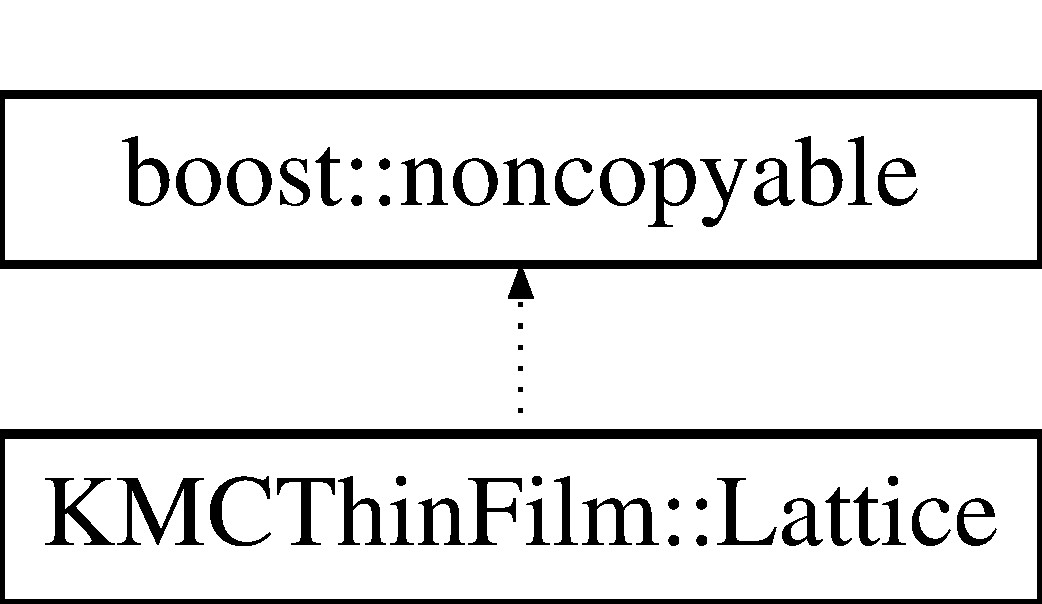
\includegraphics[height=2.000000cm]{classKMCThinFilm_1_1Lattice}
\end{center}
\end{figure}
\doxysubsubsection*{Public Member Functions}
\begin{DoxyCompactItemize}
\item 
\mbox{\hyperlink{classKMCThinFilm_1_1Lattice_ae8e2c418fc3fd1bcd0ca61c3647d6462}{Lattice}} (const \mbox{\hyperlink{structKMCThinFilm_1_1LatticeParams}{Lattice\+Params}} \&params\+For\+Lattice)
\item 
void \mbox{\hyperlink{classKMCThinFilm_1_1Lattice_aa36bda22ed2b0bc8d8737d3d63009765}{add\+Planes}} (int num\+Planes\+To\+Add)
\item 
bool \mbox{\hyperlink{classKMCThinFilm_1_1Lattice_a22bdff6d2d8478783350f84ccd73ba70}{add\+To\+Export\+Buffer\+If\+Needed}} (const \mbox{\hyperlink{classKMCThinFilm_1_1CellInds}{Cell\+Inds}} \&ci)
\item 
void \mbox{\hyperlink{classKMCThinFilm_1_1Lattice_a5cb4134926e0f9d17dc4ee0a9606d98a}{clear\+Ghosts\+To\+Send}} ()
\item 
const MPI\+\_\+\+Comm \& \mbox{\hyperlink{classKMCThinFilm_1_1Lattice_aef0511e825e463bc1f91df0720513c86}{comm}} () const
\item 
int \mbox{\hyperlink{classKMCThinFilm_1_1Lattice_a0236ed2c0c17d92a5ab01f61519f8983}{comm\+Coord}} (int dim) const
\item 
int \mbox{\hyperlink{classKMCThinFilm_1_1Lattice_a79fcfbbdb100a422553f1648019aab1a}{curr\+Height}} () const
\item 
double \mbox{\hyperlink{classKMCThinFilm_1_1Lattice_a825ef41025b740e190d60d097f9d9ae5}{get\+Float}} (const \mbox{\hyperlink{classKMCThinFilm_1_1CellInds}{Cell\+Inds}} \&ci, int which\+Float) const
\item 
void \mbox{\hyperlink{classKMCThinFilm_1_1Lattice_ac160d406b29dc80fb72551ad3d74ac3a}{get\+Global\+Planar\+BBox}} (\mbox{\hyperlink{structKMCThinFilm_1_1LatticePlanarBBox}{Lattice\+Planar\+BBox}} \&bbox) const
\item 
int \mbox{\hyperlink{classKMCThinFilm_1_1Lattice_aff659b471f414c579a51fe280b218ef1}{get\+Int}} (const \mbox{\hyperlink{classKMCThinFilm_1_1CellInds}{Cell\+Inds}} \&ci, int which\+Int) const
\item 
void \mbox{\hyperlink{classKMCThinFilm_1_1Lattice_a1504ff860e046a8965b37dd437a74c52}{get\+Local\+Planar\+BBox}} (bool w\+Ghost, \mbox{\hyperlink{structKMCThinFilm_1_1LatticePlanarBBox}{Lattice\+Planar\+BBox}} \&bbox) const
\item 
const std\+::vector$<$ std\+::vector$<$ IJK $>$ $>$ \& \mbox{\hyperlink{classKMCThinFilm_1_1Lattice_afc38b275efbadecc0800d5b77ad8841d}{get\+Received\+Ghost\+Inds}} () const
\item 
const std\+::vector$<$ std\+::vector$<$ IJK $>$ $>$ \& \mbox{\hyperlink{classKMCThinFilm_1_1Lattice_a7b1f19702b428a80fe886a5d24ae4f05}{get\+Received\+Local\+Inds}} () const
\item 
void \mbox{\hyperlink{classKMCThinFilm_1_1Lattice_ae6d9adbfdcd256875c8b9b6b281c648c}{get\+Sector\+Planar\+BBox}} (int sect\+Num, \mbox{\hyperlink{structKMCThinFilm_1_1LatticePlanarBBox}{Lattice\+Planar\+BBox}} \&bbox) const
\item 
int \mbox{\hyperlink{classKMCThinFilm_1_1Lattice_ab88c96bfe79958ad29842a6ce72c77a8}{ghost\+Extent}} (int dim) const
\item 
int \mbox{\hyperlink{classKMCThinFilm_1_1Lattice_af88c2bfaa3f80c7efc19402c0d24a50b}{n\+Floats\+Per\+Cell}} () const
\item 
int \mbox{\hyperlink{classKMCThinFilm_1_1Lattice_ae141f7cd71bbbdf12dffe12e0dc0f115}{n\+Ints\+Per\+Cell}} () const
\item 
int \mbox{\hyperlink{classKMCThinFilm_1_1Lattice_ad48a237aac1ffb943bf8b49de148da89}{n\+Procs}} () const
\item 
int \mbox{\hyperlink{classKMCThinFilm_1_1Lattice_a3bf12bd319b270be69241404305470ca}{num\+Sectors}} () const
\item 
int \mbox{\hyperlink{classKMCThinFilm_1_1Lattice_ab3e6a5e45049adf3e15a9716eae02de1}{planes\+Reserved}} () const
\item 
int \mbox{\hyperlink{classKMCThinFilm_1_1Lattice_aec4668447dc65f0a0be67b53519db0d5}{proc\+ID}} () const
\item 
int \mbox{\hyperlink{classKMCThinFilm_1_1Lattice_ab21e3aa48b60071c245ac1d3e4c8b6d9}{proc\+Per\+Dim}} (int dim) const
\item 
void \mbox{\hyperlink{classKMCThinFilm_1_1Lattice_ae6ed07b1fe933e225797e516d3a4f776}{recv\+Ghosts}} (int sect\+Num)
\item 
void \mbox{\hyperlink{classKMCThinFilm_1_1Lattice_a453210b26b7b82606bb10c3f1029cdad}{recv\+Ghosts\+Update}} (int sect\+Num)
\item 
void \mbox{\hyperlink{classKMCThinFilm_1_1Lattice_ae7545e7f3d017242dd25d7ee7dd71458}{reserve\+Planes}} (int num\+Total\+Planes\+To\+Reserve)
\item 
int \mbox{\hyperlink{classKMCThinFilm_1_1Lattice_a51bd26f57ef3eb7ba005eb2a4570478e}{sector\+Of\+Indices}} (const \mbox{\hyperlink{classKMCThinFilm_1_1CellInds}{Cell\+Inds}} \&ci) const
\item 
void \mbox{\hyperlink{classKMCThinFilm_1_1Lattice_ac4c58a1cfa17486667fe07f2cfa167cb}{send\+Ghosts}} (int sect\+Num)
\item 
void \mbox{\hyperlink{classKMCThinFilm_1_1Lattice_a11f64bd02c9f4d55da74388d69d3d0bb}{send\+Ghosts\+Update}} (int sect\+Num)
\item 
void \mbox{\hyperlink{classKMCThinFilm_1_1Lattice_aefe9601bf62fdb46d451d61fa017e691}{set\+Float}} (const \mbox{\hyperlink{classKMCThinFilm_1_1CellInds}{Cell\+Inds}} \&ci, int which\+Int, double val)
\item 
void \mbox{\hyperlink{classKMCThinFilm_1_1Lattice_a81beda29c4c8722cb047f7f2ce0a09ce}{set\+Int}} (const \mbox{\hyperlink{classKMCThinFilm_1_1CellInds}{Cell\+Inds}} \&ci, int which\+Int, int val)
\item 
int \mbox{\hyperlink{classKMCThinFilm_1_1Lattice_ad86c9013774b072638db5527ced49cf8}{wrapI}} (const \mbox{\hyperlink{classKMCThinFilm_1_1CellInds}{Cell\+Inds}} \&ci) const
\item 
int \mbox{\hyperlink{classKMCThinFilm_1_1Lattice_a837c173e46cb56875b02dbdb27da71c9}{wrapJ}} (const \mbox{\hyperlink{classKMCThinFilm_1_1CellInds}{Cell\+Inds}} \&ci) const
\end{DoxyCompactItemize}
\doxysubsubsection*{Friends}
\begin{DoxyCompactItemize}
\item 
\Hypertarget{classKMCThinFilm_1_1Lattice_aeb51e0a4c44d4192cfbdb79598859172}\label{classKMCThinFilm_1_1Lattice_aeb51e0a4c44d4192cfbdb79598859172} 
class {\bfseries Simulation}
\end{DoxyCompactItemize}


\doxysubsection{Detailed Description}
A lattice that may be distributed over several processors.

This lattice is designed to be simple but general. It is represented as a three-\/dimensional array, which can not only be used for square or simple cubic lattices, but also lattices of other physical shapes, such as the part of layer {\itshape k} of a simple hexagonal lattice shown below\+:

\begin{DoxyVerb}    (0,1,k)-----(1,1,k)----(2,1,k)----(3,1,k)---(4,1,k)
      / \        / \        / \        / \        /
     /   \      /   \      /   \      /   \      /
    /     \    /     \    /     \    /     \    /
   /       \  /       \  /       \  /       \  /
  /_________\/_________\/_________\/_________\/
(0,0,k)   (1,0,k)   (2,0,k)     (3,0,k)   (4,0,k)
\end{DoxyVerb}


For further flexibility, each site may effectively contain an array of integers and/or an array of double-\/precision floating point numbers. The lengths of these arrays is the same for all sites on the lattice. \begin{Desc}
\item[Examples]\par
\mbox{\hyperlink{testBallisticDep1_2EventsAndActions_8cpp-example}{test\+Ballistic\+Dep1/\+Events\+And\+Actions.\+cpp}}, \mbox{\hyperlink{testBallisticDep1_2EventsAndActions_8hpp-example}{test\+Ballistic\+Dep1/\+Events\+And\+Actions.\+hpp}}, \mbox{\hyperlink{testBallisticDep1_2InitLattice_8cpp-example}{test\+Ballistic\+Dep1/\+Init\+Lattice.\+cpp}}, \mbox{\hyperlink{testBallisticDep1_2InitLattice_8hpp-example}{test\+Ballistic\+Dep1/\+Init\+Lattice.\+hpp}}, \mbox{\hyperlink{testBallisticDep2_2EventsAndActions_8cpp-example}{test\+Ballistic\+Dep2/\+Events\+And\+Actions.\+cpp}}, \mbox{\hyperlink{testBallisticDep2_2EventsAndActions_8hpp-example}{test\+Ballistic\+Dep2/\+Events\+And\+Actions.\+hpp}}, \mbox{\hyperlink{testFractal_2EventsAndActions_8cpp-example}{test\+Fractal/\+Events\+And\+Actions.\+cpp}}, \mbox{\hyperlink{testFractal_2EventsAndActions_8hpp-example}{test\+Fractal/\+Events\+And\+Actions.\+hpp}}, \mbox{\hyperlink{testFractal_semi_manual_track_2EventsAndActions_8cpp-example}{test\+Fractal\+\_\+semi\+\_\+manual\+\_\+track/\+Events\+And\+Actions.\+cpp}}, \mbox{\hyperlink{testFractal_semi_manual_track_2EventsAndActions_8hpp-example}{test\+Fractal\+\_\+semi\+\_\+manual\+\_\+track/\+Events\+And\+Actions.\+hpp}}, \mbox{\hyperlink{testPatternedSurface1_2EventsAndActions_8cpp-example}{test\+Patterned\+Surface1/\+Events\+And\+Actions.\+cpp}}, \mbox{\hyperlink{testPatternedSurface1_2EventsAndActions_8hpp-example}{test\+Patterned\+Surface1/\+Events\+And\+Actions.\+hpp}}, \mbox{\hyperlink{testPatternedSurface1_2InitLattice_8cpp-example}{test\+Patterned\+Surface1/\+Init\+Lattice.\+cpp}}, \mbox{\hyperlink{testPatternedSurface1_2InitLattice_8hpp-example}{test\+Patterned\+Surface1/\+Init\+Lattice.\+hpp}}, \mbox{\hyperlink{testPatternedSurface2_2EventsAndActions_8cpp-example}{test\+Patterned\+Surface2/\+Events\+And\+Actions.\+cpp}}, and \mbox{\hyperlink{testPatternedSurface2_2EventsAndActions_8hpp-example}{test\+Patterned\+Surface2/\+Events\+And\+Actions.\+hpp}}.\end{Desc}


\doxysubsection{Constructor \& Destructor Documentation}
\Hypertarget{classKMCThinFilm_1_1Lattice_ae8e2c418fc3fd1bcd0ca61c3647d6462}\index{KMCThinFilm::Lattice@{KMCThinFilm::Lattice}!Lattice@{Lattice}}
\index{Lattice@{Lattice}!KMCThinFilm::Lattice@{KMCThinFilm::Lattice}}
\doxysubsubsection{\texorpdfstring{Lattice()}{Lattice()}}
{\footnotesize\ttfamily \label{classKMCThinFilm_1_1Lattice_ae8e2c418fc3fd1bcd0ca61c3647d6462} 
KMCThin\+Film\+::\+Lattice\+::\+Lattice (\begin{DoxyParamCaption}\item[{const \mbox{\hyperlink{structKMCThinFilm_1_1LatticeParams}{Lattice\+Params}} \&}]{params\+For\+Lattice}{}\end{DoxyParamCaption})}

\mbox{[}{\bfseries{ADVANCED}}\mbox{]} Constructor of a \doxylink{classKMCThinFilm_1_1Lattice}{Lattice} object

Unless one is debugging or testing an application that uses ARL \doxylink{namespaceKMCThinFilm}{KMCThin\+Film}, there is little point in calling this directly, since when a \doxylink{classKMCThinFilm_1_1Simulation}{Simulation} object is constructed, it builds a \doxylink{classKMCThinFilm_1_1Lattice}{Lattice} object internally for its own use. 

\doxysubsection{Member Function Documentation}
\Hypertarget{classKMCThinFilm_1_1Lattice_aa36bda22ed2b0bc8d8737d3d63009765}\index{KMCThinFilm::Lattice@{KMCThinFilm::Lattice}!addPlanes@{addPlanes}}
\index{addPlanes@{addPlanes}!KMCThinFilm::Lattice@{KMCThinFilm::Lattice}}
\doxysubsubsection{\texorpdfstring{addPlanes()}{addPlanes()}}
{\footnotesize\ttfamily \label{classKMCThinFilm_1_1Lattice_aa36bda22ed2b0bc8d8737d3d63009765} 
void KMCThin\+Film\+::\+Lattice\+::add\+Planes (\begin{DoxyParamCaption}\item[{int}]{num\+Planes\+To\+Add}{}\end{DoxyParamCaption})}

Adds zero or more layers to a given lattice, increasing the maximum value of the third lattice cell coordinate.

Note that if {\itshape num\+Planes\+To\+Add} is non-\/positive, this member function does nothing. This behavior may be used to conditionally add lattice planes. For example,


\begin{DoxyCode}{0}
\DoxyCodeLine{\textcolor{comment}{//\ Lattice\ object\ named\ "{}lattice"{}\ defined\ above}}
\DoxyCodeLine{}
\DoxyCodeLine{CellInds\ ci;}
\DoxyCodeLine{}
\DoxyCodeLine{\textcolor{comment}{//\ Misc.\ calcs\ ...}}
\DoxyCodeLine{}
\DoxyCodeLine{ci.k\ =\ someFunction(...);}
\DoxyCodeLine{kMax\ =\ lattice.currHeight()\ -\/\ 1;}
\DoxyCodeLine{}
\DoxyCodeLine{lattice.addPlanes(ci.k\ -\/\ kMax);\ \textcolor{comment}{//\ Only\ adds\ a\ lattice\ plane\ if\ ci.k\ exceeds\ kMax}}
\DoxyCodeLine{}
\DoxyCodeLine{lattice.setInt(ci,\ whichInt,\ anotherFunction(...));}

\end{DoxyCode}
 \begin{Desc}
\item[Examples]\par
\mbox{\hyperlink{testBallisticDep1_2EventsAndActions_8cpp-example}{test\+Ballistic\+Dep1/\+Events\+And\+Actions.\+cpp}}, and \mbox{\hyperlink{testPatternedSurface1_2InitLattice_8cpp-example}{test\+Patterned\+Surface1/\+Init\+Lattice.\+cpp}}.\end{Desc}
\Hypertarget{classKMCThinFilm_1_1Lattice_a22bdff6d2d8478783350f84ccd73ba70}\index{KMCThinFilm::Lattice@{KMCThinFilm::Lattice}!addToExportBufferIfNeeded@{addToExportBufferIfNeeded}}
\index{addToExportBufferIfNeeded@{addToExportBufferIfNeeded}!KMCThinFilm::Lattice@{KMCThinFilm::Lattice}}
\doxysubsubsection{\texorpdfstring{addToExportBufferIfNeeded()}{addToExportBufferIfNeeded()}}
{\footnotesize\ttfamily \label{classKMCThinFilm_1_1Lattice_a22bdff6d2d8478783350f84ccd73ba70} 
bool KMCThin\+Film\+::\+Lattice\+::add\+To\+Export\+Buffer\+If\+Needed (\begin{DoxyParamCaption}\item[{const \mbox{\hyperlink{classKMCThinFilm_1_1CellInds}{Cell\+Inds}} \&}]{ci}{}\end{DoxyParamCaption})}

\mbox{[}{\bfseries{ADVANCED}}\mbox{]} Adds {\itshape ci} to the lists of \doxylink{classKMCThinFilm_1_1CellInds}{Cell\+Inds} objects to be sent to other processors, provided that {\itshape ci} is either in a ghost region or in the part of the boundary of the lattice that is sent to other processors. Returns true if {\itshape ci} is in a ghost region.

This should typically be used between a pair of calls to \doxylink{classKMCThinFilm_1_1Lattice_a453210b26b7b82606bb10c3f1029cdad}{recv\+Ghosts\+Update(i)} and \doxylink{classKMCThinFilm_1_1Lattice_a11f64bd02c9f4d55da74388d69d3d0bb}{send\+Ghosts\+Update(i)}, where the value of {\itshape i} is the same for both calls. If ghosts are never exported, then \doxylink{classKMCThinFilm_1_1Lattice_a5cb4134926e0f9d17dc4ee0a9606d98a}{clear\+Ghosts\+To\+Send()} should be used in place of \doxylink{classKMCThinFilm_1_1Lattice_a11f64bd02c9f4d55da74388d69d3d0bb}{send\+Ghosts\+Update()}, and calls to \doxylink{classKMCThinFilm_1_1Lattice_a22bdff6d2d8478783350f84ccd73ba70}{add\+To\+Export\+Buffer\+If\+Needed()} may be called before any calls to \doxylink{classKMCThinFilm_1_1Lattice_a453210b26b7b82606bb10c3f1029cdad}{recv\+Ghosts\+Update()}. \Hypertarget{classKMCThinFilm_1_1Lattice_a5cb4134926e0f9d17dc4ee0a9606d98a}\index{KMCThinFilm::Lattice@{KMCThinFilm::Lattice}!clearGhostsToSend@{clearGhostsToSend}}
\index{clearGhostsToSend@{clearGhostsToSend}!KMCThinFilm::Lattice@{KMCThinFilm::Lattice}}
\doxysubsubsection{\texorpdfstring{clearGhostsToSend()}{clearGhostsToSend()}}
{\footnotesize\ttfamily \label{classKMCThinFilm_1_1Lattice_a5cb4134926e0f9d17dc4ee0a9606d98a} 
void KMCThin\+Film\+::\+Lattice\+::clear\+Ghosts\+To\+Send (\begin{DoxyParamCaption}{}{}\end{DoxyParamCaption})}

\mbox{[}{\bfseries{ADVANCED}}\mbox{]} Clears any ghosts that would be sent by a call to \doxylink{classKMCThinFilm_1_1Lattice_a11f64bd02c9f4d55da74388d69d3d0bb}{send\+Ghosts\+Update()} \Hypertarget{classKMCThinFilm_1_1Lattice_aef0511e825e463bc1f91df0720513c86}\index{KMCThinFilm::Lattice@{KMCThinFilm::Lattice}!comm@{comm}}
\index{comm@{comm}!KMCThinFilm::Lattice@{KMCThinFilm::Lattice}}
\doxysubsubsection{\texorpdfstring{comm()}{comm()}}
{\footnotesize\ttfamily \label{classKMCThinFilm_1_1Lattice_aef0511e825e463bc1f91df0720513c86} 
const MPI\+\_\+\+Comm \& KMCThin\+Film\+::\+Lattice\+::comm (\begin{DoxyParamCaption}{}{}\end{DoxyParamCaption}) const}

The MPI communicator used by the lattice for interchange of ghosts, if the preprocessor variable KMC\+\_\+\+PARALLEL is non-\/zero. {\bfseries{Not available in the serial version of the ARL \doxylink{namespaceKMCThinFilm}{KMCThin\+Film} library.}}

This is {\itshape not} the same as the {\itshape lattice\+Comm\+Initial} member of the \doxylink{structKMCThinFilm_1_1LatticeParams}{Lattice\+Params} object used to construct the lattice. While it contains the same number of processors as {\itshape lattice\+Comm\+Initial}, the lines of code


\begin{DoxyCode}{0}
\DoxyCodeLine{\textcolor{keywordtype}{int}\ rank;}
\DoxyCodeLine{LatticeParams\ latParams;}
\DoxyCodeLine{MPI\_Comm\_rank(latParams.latticeCommInitial,\ \&rank);}

\end{DoxyCode}


and


\begin{DoxyCode}{0}
\DoxyCodeLine{\textcolor{comment}{//\ Lattice\ object\ named\ "{}lattice"{}\ defined\ above}}
\DoxyCodeLine{\textcolor{keywordtype}{int}\ rank;}
\DoxyCodeLine{MPI\_Comm\_rank(lattice.comm(),\ \&rank);}

\end{DoxyCode}


may not return the same value for {\itshape rank}. \Hypertarget{classKMCThinFilm_1_1Lattice_a0236ed2c0c17d92a5ab01f61519f8983}\index{KMCThinFilm::Lattice@{KMCThinFilm::Lattice}!commCoord@{commCoord}}
\index{commCoord@{commCoord}!KMCThinFilm::Lattice@{KMCThinFilm::Lattice}}
\doxysubsubsection{\texorpdfstring{commCoord()}{commCoord()}}
{\footnotesize\ttfamily \label{classKMCThinFilm_1_1Lattice_a0236ed2c0c17d92a5ab01f61519f8983} 
int KMCThin\+Film\+::\+Lattice\+::comm\+Coord (\begin{DoxyParamCaption}\item[{int}]{dim}{}\end{DoxyParamCaption}) const}

Coordinates for a processor in an MPI Cartesian topology along in-\/plane dimension {\itshape dim} for a given processor.

For example, if the lattice is partitioned as follows,

\begin{DoxyVerb}*-----*-----*-----*
|  3  |  4  |  5  |
*-----*-----*-----*
|  0  |  1  |  2  |
*-----*-----*-----*
\end{DoxyVerb}


where the numbers 0, 1, 2, etc., denote processor ranks, then if the MPI rank of a processor is 4, then comm\+Coord(0) returns a value of 1, and comm\+Coord(0) returns a value of 2. The coordinates for all processor ranks in the above partitioned lattice are shown below\+:

\begin{DoxyVerb}*-----*-----*-----*
|(1,0)|(1,1)|(1,2)|
*-----*-----*-----*
|(0,0)|(0,1)|(0,2)|
*-----*-----*-----*
\end{DoxyVerb}


Note that the coordinates described here are {\itshape not} the same as the coordinates of a lattice cell.

\begin{DoxySeeAlso}{See also}
\doxylink{classKMCThinFilm_1_1Lattice_ab21e3aa48b60071c245ac1d3e4c8b6d9}{proc\+Per\+Dim()} 
\end{DoxySeeAlso}
\Hypertarget{classKMCThinFilm_1_1Lattice_a79fcfbbdb100a422553f1648019aab1a}\index{KMCThinFilm::Lattice@{KMCThinFilm::Lattice}!currHeight@{currHeight}}
\index{currHeight@{currHeight}!KMCThinFilm::Lattice@{KMCThinFilm::Lattice}}
\doxysubsubsection{\texorpdfstring{currHeight()}{currHeight()}}
{\footnotesize\ttfamily \label{classKMCThinFilm_1_1Lattice_a79fcfbbdb100a422553f1648019aab1a} 
int KMCThin\+Film\+::\+Lattice\+::curr\+Height (\begin{DoxyParamCaption}{}{}\end{DoxyParamCaption}) const}

The current number of lattice planes.

This is also one larger than the maximum value of the third lattice coordinate.

\begin{DoxySeeAlso}{See also}
\doxylink{classKMCThinFilm_1_1Lattice_a1504ff860e046a8965b37dd437a74c52}{get\+Local\+Planar\+BBox()} \doxylink{classKMCThinFilm_1_1Lattice_ae6d9adbfdcd256875c8b9b6b281c648c}{get\+Sector\+Planar\+BBox()} 
\end{DoxySeeAlso}
\begin{Desc}
\item[Examples]\par
\mbox{\hyperlink{testBallisticDep1_2EventsAndActions_8cpp-example}{test\+Ballistic\+Dep1/\+Events\+And\+Actions.\+cpp}}, and \mbox{\hyperlink{testBallisticDep2_2EventsAndActions_8cpp-example}{test\+Ballistic\+Dep2/\+Events\+And\+Actions.\+cpp}}.\end{Desc}
\Hypertarget{classKMCThinFilm_1_1Lattice_a825ef41025b740e190d60d097f9d9ae5}\index{KMCThinFilm::Lattice@{KMCThinFilm::Lattice}!getFloat@{getFloat}}
\index{getFloat@{getFloat}!KMCThinFilm::Lattice@{KMCThinFilm::Lattice}}
\doxysubsubsection{\texorpdfstring{getFloat()}{getFloat()}}
{\footnotesize\ttfamily \label{classKMCThinFilm_1_1Lattice_a825ef41025b740e190d60d097f9d9ae5} 
double KMCThin\+Film\+::\+Lattice\+::get\+Float (\begin{DoxyParamCaption}\item[{const \mbox{\hyperlink{classKMCThinFilm_1_1CellInds}{Cell\+Inds}} \&}]{ci}{, }\item[{int}]{which\+Float}{}\end{DoxyParamCaption}) const}

Returns the value of double-\/precision array element {\itshape which\+Float} at lattice cell indices {\itshape ci}.

The value of {\itshape which\+Float} ranges from 0 to \doxylink{classKMCThinFilm_1_1Lattice_af88c2bfaa3f80c7efc19402c0d24a50b}{n\+Floats\+Per\+Cell()} -\/ 1.

\begin{DoxySeeAlso}{See also}
\doxylink{classKMCThinFilm_1_1Lattice_aff659b471f414c579a51fe280b218ef1}{get\+Int()} \doxylink{classKMCThinFilm_1_1Lattice_aefe9601bf62fdb46d451d61fa017e691}{set\+Float()} \doxylink{classKMCThinFilm_1_1Lattice_a81beda29c4c8722cb047f7f2ce0a09ce}{set\+Int()} 
\end{DoxySeeAlso}
\begin{Desc}
\item[Examples]\par
\mbox{\hyperlink{testBallisticDep1_2EventsAndActions_8cpp-example}{test\+Ballistic\+Dep1/\+Events\+And\+Actions.\+cpp}}, and \mbox{\hyperlink{testBallisticDep2_2EventsAndActions_8cpp-example}{test\+Ballistic\+Dep2/\+Events\+And\+Actions.\+cpp}}.\end{Desc}
\Hypertarget{classKMCThinFilm_1_1Lattice_ac160d406b29dc80fb72551ad3d74ac3a}\index{KMCThinFilm::Lattice@{KMCThinFilm::Lattice}!getGlobalPlanarBBox@{getGlobalPlanarBBox}}
\index{getGlobalPlanarBBox@{getGlobalPlanarBBox}!KMCThinFilm::Lattice@{KMCThinFilm::Lattice}}
\doxysubsubsection{\texorpdfstring{getGlobalPlanarBBox()}{getGlobalPlanarBBox()}}
{\footnotesize\ttfamily \label{classKMCThinFilm_1_1Lattice_ac160d406b29dc80fb72551ad3d74ac3a} 
void KMCThin\+Film\+::\+Lattice\+::get\+Global\+Planar\+BBox (\begin{DoxyParamCaption}\item[{\mbox{\hyperlink{structKMCThinFilm_1_1LatticePlanarBBox}{Lattice\+Planar\+BBox}} \&}]{bbox}{}\end{DoxyParamCaption}) const}

Obtain limiting values of the global lattice coordinates.

"{}\+BBox"{} here is short for "{}bounding box."{}

Note that this function in general {\itshape cannot} be used to determine lattice coordinate values for use with \doxylink{classKMCThinFilm_1_1Lattice_aff659b471f414c579a51fe280b218ef1}{get\+Int()}, \doxylink{classKMCThinFilm_1_1Lattice_a81beda29c4c8722cb047f7f2ce0a09ce}{set\+Int()}, \doxylink{classKMCThinFilm_1_1Lattice_a825ef41025b740e190d60d097f9d9ae5}{get\+Float()}, and \doxylink{classKMCThinFilm_1_1Lattice_aefe9601bf62fdb46d451d61fa017e691}{set\+Float()}, since those functions require local lattice coordinates. To obtain limiting values for local lattice coordinates, use \doxylink{classKMCThinFilm_1_1Lattice_a1504ff860e046a8965b37dd437a74c52}{get\+Local\+Planar\+BBox()} or \doxylink{classKMCThinFilm_1_1Lattice_ae6d9adbfdcd256875c8b9b6b281c648c}{get\+Sector\+Planar\+BBox()} instead.

\begin{DoxySeeAlso}{See also}
\doxylink{classKMCThinFilm_1_1Lattice_a1504ff860e046a8965b37dd437a74c52}{get\+Local\+Planar\+BBox()} \doxylink{classKMCThinFilm_1_1Lattice_ae6d9adbfdcd256875c8b9b6b281c648c}{get\+Sector\+Planar\+BBox()} 
\end{DoxySeeAlso}

\begin{DoxyParams}{Parameters}
{\em bbox} & Bounding box of the global lattice coordinates. \\
\hline
\end{DoxyParams}
\begin{Desc}
\item[Examples]\par
\mbox{\hyperlink{testPatternedSurface1_2InitLattice_8cpp-example}{test\+Patterned\+Surface1/\+Init\+Lattice.\+cpp}}.\end{Desc}
\Hypertarget{classKMCThinFilm_1_1Lattice_aff659b471f414c579a51fe280b218ef1}\index{KMCThinFilm::Lattice@{KMCThinFilm::Lattice}!getInt@{getInt}}
\index{getInt@{getInt}!KMCThinFilm::Lattice@{KMCThinFilm::Lattice}}
\doxysubsubsection{\texorpdfstring{getInt()}{getInt()}}
{\footnotesize\ttfamily \label{classKMCThinFilm_1_1Lattice_aff659b471f414c579a51fe280b218ef1} 
int KMCThin\+Film\+::\+Lattice\+::get\+Int (\begin{DoxyParamCaption}\item[{const \mbox{\hyperlink{classKMCThinFilm_1_1CellInds}{Cell\+Inds}} \&}]{ci}{, }\item[{int}]{which\+Int}{}\end{DoxyParamCaption}) const}

Returns the value of integer array element {\itshape which\+Int} at lattice cell indices {\itshape ci}.

The value of {\itshape which\+Int} ranges from 0 to \doxylink{classKMCThinFilm_1_1Lattice_ae141f7cd71bbbdf12dffe12e0dc0f115}{n\+Ints\+Per\+Cell()} -\/ 1.

\begin{DoxySeeAlso}{See also}
\doxylink{classKMCThinFilm_1_1Lattice_a825ef41025b740e190d60d097f9d9ae5}{get\+Float()} \doxylink{classKMCThinFilm_1_1Lattice_aefe9601bf62fdb46d451d61fa017e691}{set\+Float()} \doxylink{classKMCThinFilm_1_1Lattice_a81beda29c4c8722cb047f7f2ce0a09ce}{set\+Int()} 
\end{DoxySeeAlso}
\begin{Desc}
\item[Examples]\par
\mbox{\hyperlink{testBallisticDep1_2EventsAndActions_8cpp-example}{test\+Ballistic\+Dep1/\+Events\+And\+Actions.\+cpp}}, \mbox{\hyperlink{testBallisticDep2_2EventsAndActions_8cpp-example}{test\+Ballistic\+Dep2/\+Events\+And\+Actions.\+cpp}}, \mbox{\hyperlink{testFractal_2EventsAndActions_8cpp-example}{test\+Fractal/\+Events\+And\+Actions.\+cpp}}, \mbox{\hyperlink{testFractal_semi_manual_track_2EventsAndActions_8cpp-example}{test\+Fractal\+\_\+semi\+\_\+manual\+\_\+track/\+Events\+And\+Actions.\+cpp}}, \mbox{\hyperlink{testPatternedSurface1_2EventsAndActions_8cpp-example}{test\+Patterned\+Surface1/\+Events\+And\+Actions.\+cpp}}, and \mbox{\hyperlink{testPatternedSurface2_2EventsAndActions_8cpp-example}{test\+Patterned\+Surface2/\+Events\+And\+Actions.\+cpp}}.\end{Desc}
\Hypertarget{classKMCThinFilm_1_1Lattice_a1504ff860e046a8965b37dd437a74c52}\index{KMCThinFilm::Lattice@{KMCThinFilm::Lattice}!getLocalPlanarBBox@{getLocalPlanarBBox}}
\index{getLocalPlanarBBox@{getLocalPlanarBBox}!KMCThinFilm::Lattice@{KMCThinFilm::Lattice}}
\doxysubsubsection{\texorpdfstring{getLocalPlanarBBox()}{getLocalPlanarBBox()}}
{\footnotesize\ttfamily \label{classKMCThinFilm_1_1Lattice_a1504ff860e046a8965b37dd437a74c52} 
void KMCThin\+Film\+::\+Lattice\+::get\+Local\+Planar\+BBox (\begin{DoxyParamCaption}\item[{bool}]{w\+Ghost}{, }\item[{\mbox{\hyperlink{structKMCThinFilm_1_1LatticePlanarBBox}{Lattice\+Planar\+BBox}} \&}]{bbox}{}\end{DoxyParamCaption}) const}

Obtain limiting values of the local lattice coordinates.

"{}\+BBox"{} here is short for "{}bounding box."{}

A typical use for this member function would be something like this\+:


\begin{DoxyCode}{0}
\DoxyCodeLine{\textcolor{comment}{//\ Lattice\ object\ named\ "{}lattice"{}\ defined\ above}}
\DoxyCodeLine{}
\DoxyCodeLine{\textcolor{keywordtype}{bool}\ includeGhosts\ =\ myBooleanFunc(...);}
\DoxyCodeLine{}
\DoxyCodeLine{LatticePlanarBBox\ localPlanarBBox;\ \ \ \ \ \ }
\DoxyCodeLine{lattice.getLocalPlanarBBox(includeGhosts,\ localPlanarBBox);}
\DoxyCodeLine{kMaxP1\ =\ lattice.currHeight();}
\DoxyCodeLine{}
\DoxyCodeLine{CellInds\ ci;}
\DoxyCodeLine{\textcolor{keywordflow}{for}\ (ci.k\ =\ 0;\ ci.k\ <\ kMaxP1;\ ++(ci.k))\ \{}
\DoxyCodeLine{\ \ \ \textcolor{keywordflow}{for}\ (ci.i\ =\ localPlanarBBox.imin;\ ci.i\ <\ localPlanarBBox.imaxP1;\ ++(ci.i))\ \{}
\DoxyCodeLine{\ \ \ \ \ \ \textcolor{keywordflow}{for}\ (ci.j\ =\ localPlanarBBox.jmin;\ ci.j\ <\ localPlanarBBox.jmaxP1;\ ++(ci.j))\ \{}
\DoxyCodeLine{}
\DoxyCodeLine{\ \ \ \ \ \ \ \ \ \textcolor{comment}{//\ Some\ calcs\ ...}}
\DoxyCodeLine{\ \ \ \ \ \ }
\DoxyCodeLine{\ \ \ \ \ \ \ \ \ lattice.setInt(ci,\ WHICH\_INT,\ someFunc(...));\ \ \ \ \ \ \ \ \ \ \ \ \ \ \ }
\DoxyCodeLine{\ \ \ \ \ \ \ \ \ }
\DoxyCodeLine{\ \ \ \ \ \ \ \ \ \textcolor{comment}{//\ Other\ calcs\ ...}}
\DoxyCodeLine{}
\DoxyCodeLine{\ \ \ \ \ \}}
\DoxyCodeLine{\ \ \ \}}
\DoxyCodeLine{\}}

\end{DoxyCode}


\begin{DoxySeeAlso}{See also}
\doxylink{classKMCThinFilm_1_1Lattice_ae6d9adbfdcd256875c8b9b6b281c648c}{get\+Sector\+Planar\+BBox()} \doxylink{classKMCThinFilm_1_1Lattice_ac160d406b29dc80fb72551ad3d74ac3a}{get\+Global\+Planar\+BBox()} 
\end{DoxySeeAlso}

\begin{DoxyParams}{Parameters}
{\em w\+Ghost} & Indicates whether minimum and maximum values for lattice cell coordinates include the coordinates of ghost lattice cells.  \\
\hline
{\em bbox} & Bounding box of the local lattice coordinates. \\
\hline
\end{DoxyParams}
\begin{Desc}
\item[Examples]\par
\mbox{\hyperlink{testBallisticDep1_2EventsAndActions_8cpp-example}{test\+Ballistic\+Dep1/\+Events\+And\+Actions.\+cpp}}, \mbox{\hyperlink{testBallisticDep2_2EventsAndActions_8cpp-example}{test\+Ballistic\+Dep2/\+Events\+And\+Actions.\+cpp}}, \mbox{\hyperlink{testFractal_2EventsAndActions_8cpp-example}{test\+Fractal/\+Events\+And\+Actions.\+cpp}}, \mbox{\hyperlink{testFractal_semi_manual_track_2EventsAndActions_8cpp-example}{test\+Fractal\+\_\+semi\+\_\+manual\+\_\+track/\+Events\+And\+Actions.\+cpp}}, \mbox{\hyperlink{testPatternedSurface1_2EventsAndActions_8cpp-example}{test\+Patterned\+Surface1/\+Events\+And\+Actions.\+cpp}}, \mbox{\hyperlink{testPatternedSurface1_2InitLattice_8cpp-example}{test\+Patterned\+Surface1/\+Init\+Lattice.\+cpp}}, and \mbox{\hyperlink{testPatternedSurface2_2EventsAndActions_8cpp-example}{test\+Patterned\+Surface2/\+Events\+And\+Actions.\+cpp}}.\end{Desc}
\Hypertarget{classKMCThinFilm_1_1Lattice_afc38b275efbadecc0800d5b77ad8841d}\index{KMCThinFilm::Lattice@{KMCThinFilm::Lattice}!getReceivedGhostInds@{getReceivedGhostInds}}
\index{getReceivedGhostInds@{getReceivedGhostInds}!KMCThinFilm::Lattice@{KMCThinFilm::Lattice}}
\doxysubsubsection{\texorpdfstring{getReceivedGhostInds()}{getReceivedGhostInds()}}
{\footnotesize\ttfamily \label{classKMCThinFilm_1_1Lattice_afc38b275efbadecc0800d5b77ad8841d} 
const std\+::vector$<$ std\+::vector$<$ IJK $>$ $>$ \& KMCThin\+Film\+::\+Lattice\+::get\+Received\+Ghost\+Inds (\begin{DoxyParamCaption}{}{}\end{DoxyParamCaption}) const}

\mbox{[}{\bfseries{ADVANCED}}\mbox{]} Returns the lists of the indices of cells that are changed by the latest call to \doxylink{classKMCThinFilm_1_1Lattice_a453210b26b7b82606bb10c3f1029cdad}{recv\+Ghosts\+Update()}. \Hypertarget{classKMCThinFilm_1_1Lattice_a7b1f19702b428a80fe886a5d24ae4f05}\index{KMCThinFilm::Lattice@{KMCThinFilm::Lattice}!getReceivedLocalInds@{getReceivedLocalInds}}
\index{getReceivedLocalInds@{getReceivedLocalInds}!KMCThinFilm::Lattice@{KMCThinFilm::Lattice}}
\doxysubsubsection{\texorpdfstring{getReceivedLocalInds()}{getReceivedLocalInds()}}
{\footnotesize\ttfamily \label{classKMCThinFilm_1_1Lattice_a7b1f19702b428a80fe886a5d24ae4f05} 
const std\+::vector$<$ std\+::vector$<$ IJK $>$ $>$ \& KMCThin\+Film\+::\+Lattice\+::get\+Received\+Local\+Inds (\begin{DoxyParamCaption}{}{}\end{DoxyParamCaption}) const}

\mbox{[}{\bfseries{ADVANCED}}\mbox{]} Returns the lists of the indices of cells that are changed by the latest call to \doxylink{classKMCThinFilm_1_1Lattice_a11f64bd02c9f4d55da74388d69d3d0bb}{send\+Ghosts\+Update()}. \Hypertarget{classKMCThinFilm_1_1Lattice_ae6d9adbfdcd256875c8b9b6b281c648c}\index{KMCThinFilm::Lattice@{KMCThinFilm::Lattice}!getSectorPlanarBBox@{getSectorPlanarBBox}}
\index{getSectorPlanarBBox@{getSectorPlanarBBox}!KMCThinFilm::Lattice@{KMCThinFilm::Lattice}}
\doxysubsubsection{\texorpdfstring{getSectorPlanarBBox()}{getSectorPlanarBBox()}}
{\footnotesize\ttfamily \label{classKMCThinFilm_1_1Lattice_ae6d9adbfdcd256875c8b9b6b281c648c} 
void KMCThin\+Film\+::\+Lattice\+::get\+Sector\+Planar\+BBox (\begin{DoxyParamCaption}\item[{int}]{sect\+Num}{, }\item[{\mbox{\hyperlink{structKMCThinFilm_1_1LatticePlanarBBox}{Lattice\+Planar\+BBox}} \&}]{bbox}{}\end{DoxyParamCaption}) const}

Obtain limiting values of the local lattice coordinates for a particular sector or sublattice.

"{}\+BBox"{} here is short for "{}bounding box."{}

A typical use for this member function would be something like this\+:


\begin{DoxyCode}{0}
\DoxyCodeLine{\textcolor{comment}{//\ Lattice\ object\ named\ "{}lattice"{}\ defined\ above}}
\DoxyCodeLine{}
\DoxyCodeLine{\textcolor{keywordflow}{for}\ (\textcolor{keywordtype}{int}\ sectNum\ =\ 0;\ i\ <\ lattice.numSectors();\ ++i)\ \{}
\DoxyCodeLine{}
\DoxyCodeLine{\ \ \ lattice.recvGhosts(sectNum);}
\DoxyCodeLine{}
\DoxyCodeLine{\ \ \ LatticePlanarBBox\ sectorPlanarBBox;}
\DoxyCodeLine{\ \ \ lattice.getSectorPlanarBBox(sectNum,\ sectorPlanarBBox);}
\DoxyCodeLine{\ \ \ kMaxP1\ =\ lattice.currHeight();}
\DoxyCodeLine{}
\DoxyCodeLine{\ \ \ CellInds\ ci;}
\DoxyCodeLine{\ \ \ \textcolor{keywordflow}{for}\ (ci.k\ =\ 0;\ ci.k\ <\ kMaxP1;\ ++(ci.k))\ \{}
\DoxyCodeLine{\ \ \ \ \ \ \textcolor{keywordflow}{for}\ (ci.i\ =\ sectorPlanarBBox.imin;\ ci.i\ <\ sectorPlanarBBox.imaxP1;\ ++(ci.i))\ \{}
\DoxyCodeLine{\ \ \ \ \ \ \ \ \ \textcolor{keywordflow}{for}\ (ci.j\ =\ sectorPlanarBBox.jmin;\ ci.j\ <\ sectorPlanarBBox.jmaxP1;\ ++(ci.j))\ \{}
\DoxyCodeLine{\ \ \ \ \ \ \ \ \ \ \ \ \textcolor{comment}{//\ Some\ calcs\ ...}}
\DoxyCodeLine{\ \ \ \ \ \ }
\DoxyCodeLine{\ \ \ \ \ \ \ \ \ \ \ \ lattice.setFloat(ci,\ FLT\_VAL1,\ someFunc(...));}
\DoxyCodeLine{}
\DoxyCodeLine{\ \ \ \ \ \ \ \ \ \ \ \ \textcolor{comment}{//\ Other\ calcs\ ...}}
\DoxyCodeLine{}
\DoxyCodeLine{\ \ \ \ \ \ \ \ \}}
\DoxyCodeLine{\ \ \ \ \ \ \}}
\DoxyCodeLine{\ \ \ \}}
\DoxyCodeLine{}
\DoxyCodeLine{\ \ \ lattice.sendGhosts(sectNum);}
\DoxyCodeLine{\}}

\end{DoxyCode}


Note that unlike \doxylink{classKMCThinFilm_1_1Lattice_a1504ff860e046a8965b37dd437a74c52}{get\+Local\+Planar\+BBox()}, the minimum and maximum lattice coordinate values do not include the coordinates of ghost lattice cells.

\begin{DoxySeeAlso}{See also}
\doxylink{classKMCThinFilm_1_1Lattice_a1504ff860e046a8965b37dd437a74c52}{get\+Local\+Planar\+BBox()} \doxylink{classKMCThinFilm_1_1Lattice_ac160d406b29dc80fb72551ad3d74ac3a}{get\+Global\+Planar\+BBox()} \doxylink{classKMCThinFilm_1_1Lattice_a3bf12bd319b270be69241404305470ca}{num\+Sectors()} 
\end{DoxySeeAlso}

\begin{DoxyParams}{Parameters}
{\em sect\+Num} & Sector number, ranging from 0 to \doxylink{classKMCThinFilm_1_1Lattice_a3bf12bd319b270be69241404305470ca}{num\+Sectors()} -\/ 1  \\
\hline
{\em bbox} & Bounding box of the lattice coordinates within the sector. \\
\hline
\end{DoxyParams}
\Hypertarget{classKMCThinFilm_1_1Lattice_ab88c96bfe79958ad29842a6ce72c77a8}\index{KMCThinFilm::Lattice@{KMCThinFilm::Lattice}!ghostExtent@{ghostExtent}}
\index{ghostExtent@{ghostExtent}!KMCThinFilm::Lattice@{KMCThinFilm::Lattice}}
\doxysubsubsection{\texorpdfstring{ghostExtent()}{ghostExtent()}}
{\footnotesize\ttfamily \label{classKMCThinFilm_1_1Lattice_ab88c96bfe79958ad29842a6ce72c77a8} 
int KMCThin\+Film\+::\+Lattice\+::ghost\+Extent (\begin{DoxyParamCaption}\item[{int}]{dim}{}\end{DoxyParamCaption}) const}

Thickness of the ghost region along in-\/plane dimension {\itshape dim}.

Dimension 0 is the dimension along which the first lattice cell index varies, and dimension 1 is the dimension along which the second lattice cell index varies.

\begin{DoxySeeAlso}{See also}
\doxylink{classKMCThinFilm_1_1Lattice_a0236ed2c0c17d92a5ab01f61519f8983}{comm\+Coord()} 
\end{DoxySeeAlso}
\Hypertarget{classKMCThinFilm_1_1Lattice_af88c2bfaa3f80c7efc19402c0d24a50b}\index{KMCThinFilm::Lattice@{KMCThinFilm::Lattice}!nFloatsPerCell@{nFloatsPerCell}}
\index{nFloatsPerCell@{nFloatsPerCell}!KMCThinFilm::Lattice@{KMCThinFilm::Lattice}}
\doxysubsubsection{\texorpdfstring{nFloatsPerCell()}{nFloatsPerCell()}}
{\footnotesize\ttfamily \label{classKMCThinFilm_1_1Lattice_af88c2bfaa3f80c7efc19402c0d24a50b} 
int KMCThin\+Film\+::\+Lattice\+::n\+Floats\+Per\+Cell (\begin{DoxyParamCaption}{}{}\end{DoxyParamCaption}) const}

Length of the double-\/precision floating-\/point array at each lattice cell. \Hypertarget{classKMCThinFilm_1_1Lattice_ae141f7cd71bbbdf12dffe12e0dc0f115}\index{KMCThinFilm::Lattice@{KMCThinFilm::Lattice}!nIntsPerCell@{nIntsPerCell}}
\index{nIntsPerCell@{nIntsPerCell}!KMCThinFilm::Lattice@{KMCThinFilm::Lattice}}
\doxysubsubsection{\texorpdfstring{nIntsPerCell()}{nIntsPerCell()}}
{\footnotesize\ttfamily \label{classKMCThinFilm_1_1Lattice_ae141f7cd71bbbdf12dffe12e0dc0f115} 
int KMCThin\+Film\+::\+Lattice\+::n\+Ints\+Per\+Cell (\begin{DoxyParamCaption}{}{}\end{DoxyParamCaption}) const}

Length of the integer array at each lattice cell. \Hypertarget{classKMCThinFilm_1_1Lattice_ad48a237aac1ffb943bf8b49de148da89}\index{KMCThinFilm::Lattice@{KMCThinFilm::Lattice}!nProcs@{nProcs}}
\index{nProcs@{nProcs}!KMCThinFilm::Lattice@{KMCThinFilm::Lattice}}
\doxysubsubsection{\texorpdfstring{nProcs()}{nProcs()}}
{\footnotesize\ttfamily \label{classKMCThinFilm_1_1Lattice_ad48a237aac1ffb943bf8b49de148da89} 
int KMCThin\+Film\+::\+Lattice\+::n\+Procs (\begin{DoxyParamCaption}{}{}\end{DoxyParamCaption}) const}

Number of processors over which the lattice is distributed. \Hypertarget{classKMCThinFilm_1_1Lattice_a3bf12bd319b270be69241404305470ca}\index{KMCThinFilm::Lattice@{KMCThinFilm::Lattice}!numSectors@{numSectors}}
\index{numSectors@{numSectors}!KMCThinFilm::Lattice@{KMCThinFilm::Lattice}}
\doxysubsubsection{\texorpdfstring{numSectors()}{numSectors()}}
{\footnotesize\ttfamily \label{classKMCThinFilm_1_1Lattice_a3bf12bd319b270be69241404305470ca} 
int KMCThin\+Film\+::\+Lattice\+::num\+Sectors (\begin{DoxyParamCaption}{}{}\end{DoxyParamCaption}) const}

If the preprocessor variable KMC\+\_\+\+PARALLEL is zero, then this always returns 1. Otherwise, this is the number of sectors (or sublattices) used in the approximate parallel Kinetic Monte Carlo algorithm used by this library.

For a discussion of what these sectors are, see Y. Shim and J. G. Amar, "{}\+Semirigorous synchronous sublattice algorithm for parallel Kinetic Monte Carlo simulation of thin film growth"{}, Physical Review B, vol. 71, 125432 (2005) or S. Plimpton et al., "{}\+Crossing the Mesoscale No-\/\+Man\textquotesingle{}s Land via Parallel Kinetic Monte \+Carlo"{}, Sandia National Laboratories Technical Report SAND2009-\/6226 (2009). \Hypertarget{classKMCThinFilm_1_1Lattice_ab3e6a5e45049adf3e15a9716eae02de1}\index{KMCThinFilm::Lattice@{KMCThinFilm::Lattice}!planesReserved@{planesReserved}}
\index{planesReserved@{planesReserved}!KMCThinFilm::Lattice@{KMCThinFilm::Lattice}}
\doxysubsubsection{\texorpdfstring{planesReserved()}{planesReserved()}}
{\footnotesize\ttfamily \label{classKMCThinFilm_1_1Lattice_ab3e6a5e45049adf3e15a9716eae02de1} 
int KMCThin\+Film\+::\+Lattice\+::planes\+Reserved (\begin{DoxyParamCaption}{}{}\end{DoxyParamCaption}) const}

Returns the number of planes reserved for the lattice (but not necessarily added to the lattice yet).

Note that while this should be at least the number of planes that were explicitly reserved, it may be more than that. \Hypertarget{classKMCThinFilm_1_1Lattice_aec4668447dc65f0a0be67b53519db0d5}\index{KMCThinFilm::Lattice@{KMCThinFilm::Lattice}!procID@{procID}}
\index{procID@{procID}!KMCThinFilm::Lattice@{KMCThinFilm::Lattice}}
\doxysubsubsection{\texorpdfstring{procID()}{procID()}}
{\footnotesize\ttfamily \label{classKMCThinFilm_1_1Lattice_aec4668447dc65f0a0be67b53519db0d5} 
int KMCThin\+Film\+::\+Lattice\+::proc\+ID (\begin{DoxyParamCaption}{}{}\end{DoxyParamCaption}) const}

When the preprocessor variable KMC\+\_\+\+PARALLEL is zero, this always returns zero. Otherwise, this is the MPI rank of the local process, where the communicator for that process is given by \doxylink{classKMCThinFilm_1_1Lattice_aef0511e825e463bc1f91df0720513c86}{Lattice\+::comm()}. \Hypertarget{classKMCThinFilm_1_1Lattice_ab21e3aa48b60071c245ac1d3e4c8b6d9}\index{KMCThinFilm::Lattice@{KMCThinFilm::Lattice}!procPerDim@{procPerDim}}
\index{procPerDim@{procPerDim}!KMCThinFilm::Lattice@{KMCThinFilm::Lattice}}
\doxysubsubsection{\texorpdfstring{procPerDim()}{procPerDim()}}
{\footnotesize\ttfamily \label{classKMCThinFilm_1_1Lattice_ab21e3aa48b60071c245ac1d3e4c8b6d9} 
int KMCThin\+Film\+::\+Lattice\+::proc\+Per\+Dim (\begin{DoxyParamCaption}\item[{int}]{dim}{}\end{DoxyParamCaption}) const}

The number of processors along in-\/plane dimension {\itshape dim}.

For example, if the lattice is partitioned as follows,

\begin{DoxyVerb}*-----*-----*-----*
|  3  |  4  |  5  |
*-----*-----*-----*
|  0  |  1  |  2  |
*-----*-----*-----*
\end{DoxyVerb}


then proc\+Per\+Dim(0) returns a value of 3, and proc\+Per\+Dim(2) returns a value of 2.

\begin{DoxySeeAlso}{See also}
\doxylink{classKMCThinFilm_1_1Lattice_a0236ed2c0c17d92a5ab01f61519f8983}{comm\+Coord()} 
\end{DoxySeeAlso}
\Hypertarget{classKMCThinFilm_1_1Lattice_ae6ed07b1fe933e225797e516d3a4f776}\index{KMCThinFilm::Lattice@{KMCThinFilm::Lattice}!recvGhosts@{recvGhosts}}
\index{recvGhosts@{recvGhosts}!KMCThinFilm::Lattice@{KMCThinFilm::Lattice}}
\doxysubsubsection{\texorpdfstring{recvGhosts()}{recvGhosts()}}
{\footnotesize\ttfamily \label{classKMCThinFilm_1_1Lattice_ae6ed07b1fe933e225797e516d3a4f776} 
void KMCThin\+Film\+::\+Lattice\+::recv\+Ghosts (\begin{DoxyParamCaption}\item[{int}]{sect\+Num}{}\end{DoxyParamCaption})}

\mbox{[}{\bfseries{ADVANCED}}\mbox{]} Update {\itshape all} the ghost lattice cells from data received from other processors.

This member function does not keep track of which lattice sites are actually changed during the update, unlike \doxylink{classKMCThinFilm_1_1Lattice_a453210b26b7b82606bb10c3f1029cdad}{recv\+Ghosts\+Update()}. 
\begin{DoxyParams}{Parameters}
{\em sect\+Num} & Sector number, ranging from 0 to \doxylink{classKMCThinFilm_1_1Lattice_a3bf12bd319b270be69241404305470ca}{num\+Sectors()} -\/ 1 \\
\hline
\end{DoxyParams}
\Hypertarget{classKMCThinFilm_1_1Lattice_a453210b26b7b82606bb10c3f1029cdad}\index{KMCThinFilm::Lattice@{KMCThinFilm::Lattice}!recvGhostsUpdate@{recvGhostsUpdate}}
\index{recvGhostsUpdate@{recvGhostsUpdate}!KMCThinFilm::Lattice@{KMCThinFilm::Lattice}}
\doxysubsubsection{\texorpdfstring{recvGhostsUpdate()}{recvGhostsUpdate()}}
{\footnotesize\ttfamily \label{classKMCThinFilm_1_1Lattice_a453210b26b7b82606bb10c3f1029cdad} 
void KMCThin\+Film\+::\+Lattice\+::recv\+Ghosts\+Update (\begin{DoxyParamCaption}\item[{int}]{sect\+Num}{}\end{DoxyParamCaption})}

\mbox{[}{\bfseries{ADVANCED}}\mbox{]} Updates ghost lattice cells from data received from other processors, but only updates the cells that are supposed to have actually changed. Processors use \doxylink{classKMCThinFilm_1_1Lattice_a22bdff6d2d8478783350f84ccd73ba70}{add\+To\+Export\+Buffer\+If\+Needed()} to mark the cells that will be received by a call to this function. 
\begin{DoxyParams}{Parameters}
{\em sect\+Num} & Sector number, ranging from 0 to \doxylink{classKMCThinFilm_1_1Lattice_a3bf12bd319b270be69241404305470ca}{num\+Sectors()} -\/ 1 \\
\hline
\end{DoxyParams}
\Hypertarget{classKMCThinFilm_1_1Lattice_ae7545e7f3d017242dd25d7ee7dd71458}\index{KMCThinFilm::Lattice@{KMCThinFilm::Lattice}!reservePlanes@{reservePlanes}}
\index{reservePlanes@{reservePlanes}!KMCThinFilm::Lattice@{KMCThinFilm::Lattice}}
\doxysubsubsection{\texorpdfstring{reservePlanes()}{reservePlanes()}}
{\footnotesize\ttfamily \label{classKMCThinFilm_1_1Lattice_ae7545e7f3d017242dd25d7ee7dd71458} 
void KMCThin\+Film\+::\+Lattice\+::reserve\+Planes (\begin{DoxyParamCaption}\item[{int}]{num\+Total\+Planes\+To\+Reserve}{}\end{DoxyParamCaption})}

\mbox{[}{\bfseries{ADVANCED}}\mbox{]} Reserves space in memory for adding planes to a lattice\textsuperscript{\texorpdfstring{$\ast$}{*}}, but does not actually add any additional planes. {\bfseries{Almost certainly unnecessary if \doxylink{structKMCThinFilm_1_1LatticeParams_a1b5bd22cee6f39342f07f59fb31866c9}{Lattice\+Params\+::num\+Planes\+To\+Reserve} has been set to an appropriate value}}.

The relationship between \doxylink{classKMCThinFilm_1_1Lattice_ae7545e7f3d017242dd25d7ee7dd71458}{reserve\+Planes()} and \doxylink{classKMCThinFilm_1_1Lattice_aa36bda22ed2b0bc8d8737d3d63009765}{add\+Planes()} is somewhat analogous to that of the std\+::vector member functions reserve() and push\+\_\+back(). The former only allocates space in memory, while the latter is responsible for appending actual values (i.\+e. lattice planes). Note that if {\itshape num\+Total\+Planes\+To\+Reserve} is too small, it is not an error, though it may affect performance somewhat.

\textsuperscript{\texorpdfstring{$\ast$}{*}}Or at least pointers for those planes.

\begin{DoxySeeAlso}{See also}
\doxylink{classKMCThinFilm_1_1Lattice_aa36bda22ed2b0bc8d8737d3d63009765}{add\+Planes()} 
\end{DoxySeeAlso}
\Hypertarget{classKMCThinFilm_1_1Lattice_a51bd26f57ef3eb7ba005eb2a4570478e}\index{KMCThinFilm::Lattice@{KMCThinFilm::Lattice}!sectorOfIndices@{sectorOfIndices}}
\index{sectorOfIndices@{sectorOfIndices}!KMCThinFilm::Lattice@{KMCThinFilm::Lattice}}
\doxysubsubsection{\texorpdfstring{sectorOfIndices()}{sectorOfIndices()}}
{\footnotesize\ttfamily \label{classKMCThinFilm_1_1Lattice_a51bd26f57ef3eb7ba005eb2a4570478e} 
int KMCThin\+Film\+::\+Lattice\+::sector\+Of\+Indices (\begin{DoxyParamCaption}\item[{const \mbox{\hyperlink{classKMCThinFilm_1_1CellInds}{Cell\+Inds}} \&}]{ci}{}\end{DoxyParamCaption}) const}

Returns the sector to which a set of cell indices {\itshape ci} belongs.

If {\itshape ci} is within a ghost region, then this function returns -\/1.

In serial, this always returns zero. \Hypertarget{classKMCThinFilm_1_1Lattice_ac4c58a1cfa17486667fe07f2cfa167cb}\index{KMCThinFilm::Lattice@{KMCThinFilm::Lattice}!sendGhosts@{sendGhosts}}
\index{sendGhosts@{sendGhosts}!KMCThinFilm::Lattice@{KMCThinFilm::Lattice}}
\doxysubsubsection{\texorpdfstring{sendGhosts()}{sendGhosts()}}
{\footnotesize\ttfamily \label{classKMCThinFilm_1_1Lattice_ac4c58a1cfa17486667fe07f2cfa167cb} 
void KMCThin\+Film\+::\+Lattice\+::send\+Ghosts (\begin{DoxyParamCaption}\item[{int}]{sect\+Num}{}\end{DoxyParamCaption})}

\mbox{[}{\bfseries{ADVANCED}}\mbox{]} Send data from {\itshape all} the ghost lattice cells to update the off-\/process cells to which the ghosts correspond.

This member function does not keep track of which lattice sites are actually changed during the update, unlike \doxylink{classKMCThinFilm_1_1Lattice_a11f64bd02c9f4d55da74388d69d3d0bb}{send\+Ghosts\+Update()}. 
\begin{DoxyParams}{Parameters}
{\em sect\+Num} & Sector number, ranging from 0 to \doxylink{classKMCThinFilm_1_1Lattice_a3bf12bd319b270be69241404305470ca}{num\+Sectors()} -\/ 1 \\
\hline
\end{DoxyParams}
\Hypertarget{classKMCThinFilm_1_1Lattice_a11f64bd02c9f4d55da74388d69d3d0bb}\index{KMCThinFilm::Lattice@{KMCThinFilm::Lattice}!sendGhostsUpdate@{sendGhostsUpdate}}
\index{sendGhostsUpdate@{sendGhostsUpdate}!KMCThinFilm::Lattice@{KMCThinFilm::Lattice}}
\doxysubsubsection{\texorpdfstring{sendGhostsUpdate()}{sendGhostsUpdate()}}
{\footnotesize\ttfamily \label{classKMCThinFilm_1_1Lattice_a11f64bd02c9f4d55da74388d69d3d0bb} 
void KMCThin\+Film\+::\+Lattice\+::send\+Ghosts\+Update (\begin{DoxyParamCaption}\item[{int}]{sect\+Num}{}\end{DoxyParamCaption})}

\mbox{[}{\bfseries{ADVANCED}}\mbox{]} Sends data from the ghost lattice cells to update the (usually off-\/process) cells to which the ghosts correspond, but only updates the cells that are supposed to have actually changed. Processors use \doxylink{classKMCThinFilm_1_1Lattice_a22bdff6d2d8478783350f84ccd73ba70}{add\+To\+Export\+Buffer\+If\+Needed()} to mark the cells that will be received by a call to this function. 
\begin{DoxyParams}{Parameters}
{\em sect\+Num} & Sector number, ranging from 0 to \doxylink{classKMCThinFilm_1_1Lattice_a3bf12bd319b270be69241404305470ca}{num\+Sectors()} -\/ 1 \\
\hline
\end{DoxyParams}
\Hypertarget{classKMCThinFilm_1_1Lattice_aefe9601bf62fdb46d451d61fa017e691}\index{KMCThinFilm::Lattice@{KMCThinFilm::Lattice}!setFloat@{setFloat}}
\index{setFloat@{setFloat}!KMCThinFilm::Lattice@{KMCThinFilm::Lattice}}
\doxysubsubsection{\texorpdfstring{setFloat()}{setFloat()}}
{\footnotesize\ttfamily \label{classKMCThinFilm_1_1Lattice_aefe9601bf62fdb46d451d61fa017e691} 
void KMCThin\+Film\+::\+Lattice\+::set\+Float (\begin{DoxyParamCaption}\item[{const \mbox{\hyperlink{classKMCThinFilm_1_1CellInds}{Cell\+Inds}} \&}]{ci}{, }\item[{int}]{which\+Int}{, }\item[{double}]{val}{}\end{DoxyParamCaption})}

Sets to {\itshape val} the value of double-\/precision array element {\itshape which\+Float} at lattice cell indices {\itshape ci}.

The value of {\itshape which\+Float} ranges from 0 to \doxylink{classKMCThinFilm_1_1Lattice_af88c2bfaa3f80c7efc19402c0d24a50b}{n\+Floats\+Per\+Cell()} -\/ 1.

\begin{DoxySeeAlso}{See also}
\doxylink{classKMCThinFilm_1_1Lattice_a825ef41025b740e190d60d097f9d9ae5}{get\+Float()} \doxylink{classKMCThinFilm_1_1Lattice_aff659b471f414c579a51fe280b218ef1}{get\+Int()} \doxylink{classKMCThinFilm_1_1Lattice_a81beda29c4c8722cb047f7f2ce0a09ce}{set\+Int()} 
\end{DoxySeeAlso}
\begin{Desc}
\item[Examples]\par
\mbox{\hyperlink{testBallisticDep1_2EventsAndActions_8cpp-example}{test\+Ballistic\+Dep1/\+Events\+And\+Actions.\+cpp}}, and \mbox{\hyperlink{testPatternedSurface1_2InitLattice_8cpp-example}{test\+Patterned\+Surface1/\+Init\+Lattice.\+cpp}}.\end{Desc}
\Hypertarget{classKMCThinFilm_1_1Lattice_a81beda29c4c8722cb047f7f2ce0a09ce}\index{KMCThinFilm::Lattice@{KMCThinFilm::Lattice}!setInt@{setInt}}
\index{setInt@{setInt}!KMCThinFilm::Lattice@{KMCThinFilm::Lattice}}
\doxysubsubsection{\texorpdfstring{setInt()}{setInt()}}
{\footnotesize\ttfamily \label{classKMCThinFilm_1_1Lattice_a81beda29c4c8722cb047f7f2ce0a09ce} 
void KMCThin\+Film\+::\+Lattice\+::set\+Int (\begin{DoxyParamCaption}\item[{const \mbox{\hyperlink{classKMCThinFilm_1_1CellInds}{Cell\+Inds}} \&}]{ci}{, }\item[{int}]{which\+Int}{, }\item[{int}]{val}{}\end{DoxyParamCaption})}

Sets to {\itshape val} the value of integer array element {\itshape which\+Int} at lattice cell indices {\itshape ci}.

The value of {\itshape which\+Int} ranges from 0 to \doxylink{classKMCThinFilm_1_1Lattice_ae141f7cd71bbbdf12dffe12e0dc0f115}{n\+Ints\+Per\+Cell()} -\/ 1.

\begin{DoxySeeAlso}{See also}
\doxylink{classKMCThinFilm_1_1Lattice_a825ef41025b740e190d60d097f9d9ae5}{get\+Float()} \doxylink{classKMCThinFilm_1_1Lattice_aff659b471f414c579a51fe280b218ef1}{get\+Int()} \doxylink{classKMCThinFilm_1_1Lattice_aefe9601bf62fdb46d451d61fa017e691}{set\+Float()} 
\end{DoxySeeAlso}
\begin{Desc}
\item[Examples]\par
\mbox{\hyperlink{testBallisticDep1_2EventsAndActions_8cpp-example}{test\+Ballistic\+Dep1/\+Events\+And\+Actions.\+cpp}}, \mbox{\hyperlink{testFractal_2EventsAndActions_8cpp-example}{test\+Fractal/\+Events\+And\+Actions.\+cpp}}, \mbox{\hyperlink{testPatternedSurface1_2EventsAndActions_8cpp-example}{test\+Patterned\+Surface1/\+Events\+And\+Actions.\+cpp}}, and \mbox{\hyperlink{testPatternedSurface2_2EventsAndActions_8cpp-example}{test\+Patterned\+Surface2/\+Events\+And\+Actions.\+cpp}}.\end{Desc}
\Hypertarget{classKMCThinFilm_1_1Lattice_ad86c9013774b072638db5527ced49cf8}\index{KMCThinFilm::Lattice@{KMCThinFilm::Lattice}!wrapI@{wrapI}}
\index{wrapI@{wrapI}!KMCThinFilm::Lattice@{KMCThinFilm::Lattice}}
\doxysubsubsection{\texorpdfstring{wrapI()}{wrapI()}}
{\footnotesize\ttfamily \label{classKMCThinFilm_1_1Lattice_ad86c9013774b072638db5527ced49cf8} 
int KMCThin\+Film\+::\+Lattice\+::wrapI (\begin{DoxyParamCaption}\item[{const \mbox{\hyperlink{classKMCThinFilm_1_1CellInds}{Cell\+Inds}} \&}]{ci}{}\end{DoxyParamCaption}) const}

Returns a wrapped version of ci.\+i to account for periodic boundary conditions.

This is likely to only be useful in serial simulations.

Furthermore, the member functions \doxylink{classKMCThinFilm_1_1Lattice_aff659b471f414c579a51fe280b218ef1}{get\+Int()}, \doxylink{classKMCThinFilm_1_1Lattice_a825ef41025b740e190d60d097f9d9ae5}{get\+Float()}, \doxylink{classKMCThinFilm_1_1Lattice_a81beda29c4c8722cb047f7f2ce0a09ce}{set\+Int()}, and \doxylink{classKMCThinFilm_1_1Lattice_aefe9601bf62fdb46d451d61fa017e691}{set\+Float()} {\itshape already} account for periodic boundary conditions, so this function is mostly needed for circumstances where one is doing arithmetic of cell indices. \begin{Desc}
\item[Examples]\par
\mbox{\hyperlink{testBallisticDep2_2EventsAndActions_8cpp-example}{test\+Ballistic\+Dep2/\+Events\+And\+Actions.\+cpp}}.\end{Desc}
\Hypertarget{classKMCThinFilm_1_1Lattice_a837c173e46cb56875b02dbdb27da71c9}\index{KMCThinFilm::Lattice@{KMCThinFilm::Lattice}!wrapJ@{wrapJ}}
\index{wrapJ@{wrapJ}!KMCThinFilm::Lattice@{KMCThinFilm::Lattice}}
\doxysubsubsection{\texorpdfstring{wrapJ()}{wrapJ()}}
{\footnotesize\ttfamily \label{classKMCThinFilm_1_1Lattice_a837c173e46cb56875b02dbdb27da71c9} 
int KMCThin\+Film\+::\+Lattice\+::wrapJ (\begin{DoxyParamCaption}\item[{const \mbox{\hyperlink{classKMCThinFilm_1_1CellInds}{Cell\+Inds}} \&}]{ci}{}\end{DoxyParamCaption}) const}

Returns a wrapped version of ci.\+j to account for periodic boundary conditions.

This is likely to only be useful in serial simulations, though it perhaps may be of use if row-\/based decomposition is used in parallel simulations.

Furthermore, the member functions \doxylink{classKMCThinFilm_1_1Lattice_aff659b471f414c579a51fe280b218ef1}{get\+Int()}, \doxylink{classKMCThinFilm_1_1Lattice_a825ef41025b740e190d60d097f9d9ae5}{get\+Float()}, \doxylink{classKMCThinFilm_1_1Lattice_a81beda29c4c8722cb047f7f2ce0a09ce}{set\+Int()}, and \doxylink{classKMCThinFilm_1_1Lattice_aefe9601bf62fdb46d451d61fa017e691}{set\+Float()} {\itshape already} account for periodic boundary conditions, so this function is mostly needed for circumstances where one is doing arithmetic of cell indices. \begin{Desc}
\item[Examples]\par
\mbox{\hyperlink{testBallisticDep2_2EventsAndActions_8cpp-example}{test\+Ballistic\+Dep2/\+Events\+And\+Actions.\+cpp}}.\end{Desc}

\doxysection{KMCThin\+Film\+::Lattice\+Params Struct Reference}
\hypertarget{structKMCThinFilm_1_1LatticeParams}{}\label{structKMCThinFilm_1_1LatticeParams}\index{KMCThinFilm::LatticeParams@{KMCThinFilm::LatticeParams}}


{\ttfamily \#include $<$Lattice.\+hpp$>$}

\doxysubsubsection*{Public Types}
\begin{DoxyCompactItemize}
\item 
enum \mbox{\hyperlink{structKMCThinFilm_1_1LatticeParams_ad3f37769b5b30a8f3e941743271def8a}{Parallel\+Decomp}} \{ \mbox{\hyperlink{structKMCThinFilm_1_1LatticeParams_ad3f37769b5b30a8f3e941743271def8aa8fc91ae7961264b3e4b8a0706bc01968}{COMPACT}}
, \mbox{\hyperlink{structKMCThinFilm_1_1LatticeParams_ad3f37769b5b30a8f3e941743271def8aab4e4643da3a5463b83a72e7b9d89f5a1}{ROW}}
 \}
\end{DoxyCompactItemize}
\doxysubsubsection*{Public Attributes}
\begin{DoxyCompactItemize}
\item 
boost\+::array$<$ int, 2 $>$ \mbox{\hyperlink{structKMCThinFilm_1_1LatticeParams_addb121738727b46ba00c2c71996f4272}{ghost\+Extent}}
\item 
boost\+::array$<$ int, 2 $>$ \mbox{\hyperlink{structKMCThinFilm_1_1LatticeParams_a3a3cc62a6fb5fdda00ed2c63e1ff1020}{global\+Planar\+Dims}}
\item 
\mbox{\hyperlink{namespaceKMCThinFilm_a716044de50c29c8bb9118f8dbeb3d4bf}{Lattice\+Initializer}} \mbox{\hyperlink{structKMCThinFilm_1_1LatticeParams_a3591118c88951f3a6c7de54117979c36}{lat\+Init}}
\item 
MPI\+\_\+\+Comm \mbox{\hyperlink{structKMCThinFilm_1_1LatticeParams_aedfa8e1396eb7bc532ce63565a0f6986}{lattice\+Comm\+Initial}}
\item 
bool \mbox{\hyperlink{structKMCThinFilm_1_1LatticeParams_a4aa377013681330e14aae60bf51e0b33}{no\+Adding\+Planes\+During\+Simulation}}
\item 
int \mbox{\hyperlink{structKMCThinFilm_1_1LatticeParams_a55263f7f4ef826b814ffeaae27ddf687}{num\+Floats\+Per\+Cell}}
\item 
int \mbox{\hyperlink{structKMCThinFilm_1_1LatticeParams_a7a9d46d27758a276fd20d9c18156371a}{num\+Ints\+Per\+Cell}}
\item 
int \mbox{\hyperlink{structKMCThinFilm_1_1LatticeParams_a1b5bd22cee6f39342f07f59fb31866c9}{num\+Planes\+To\+Reserve}}
\item 
\mbox{\hyperlink{structKMCThinFilm_1_1LatticeParams_ad3f37769b5b30a8f3e941743271def8a}{Parallel\+Decomp}} \mbox{\hyperlink{structKMCThinFilm_1_1LatticeParams_a02f5a1a7568e0d94d0127260b4e9dd05}{parallel\+Decomp}}
\item 
\mbox{\hyperlink{namespaceKMCThinFilm_a92970705c2d791c5497beb06d88c8fa3}{Set\+Empty\+Cell\+Vals}} \mbox{\hyperlink{structKMCThinFilm_1_1LatticeParams_afc58fe3eed9df51a18d9a3fe2ed3b8d1}{set\+Empty\+Cell\+Vals}}
\end{DoxyCompactItemize}


\doxysubsection{Detailed Description}
Parameter object used in constructing a \doxylink{classKMCThinFilm_1_1Lattice}{Lattice} object \begin{Desc}
\item[Examples]\par
\mbox{\hyperlink{testBallisticDep1_2testBallisticDep_8cpp-example}{test\+Ballistic\+Dep1/test\+Ballistic\+Dep.\+cpp}}, \mbox{\hyperlink{testBallisticDep2_2testBallisticDep_8cpp-example}{test\+Ballistic\+Dep2/test\+Ballistic\+Dep.\+cpp}}, \mbox{\hyperlink{testFractal_2testFractal_8cpp-example}{test\+Fractal/test\+Fractal.\+cpp}}, \mbox{\hyperlink{testFractal_parallel_2testFractal_8cpp-example}{test\+Fractal\+\_\+parallel/test\+Fractal.\+cpp}}, \mbox{\hyperlink{testFractal_semi_manual_track_2testFractal_8cpp-example}{test\+Fractal\+\_\+semi\+\_\+manual\+\_\+track/test\+Fractal.\+cpp}}, \mbox{\hyperlink{testPatternedSurface1_2testPatternedSurface_8cpp-example}{test\+Patterned\+Surface1/test\+Patterned\+Surface.\+cpp}}, and \mbox{\hyperlink{testPatternedSurface2_2testPatternedSurface_8cpp-example}{test\+Patterned\+Surface2/test\+Patterned\+Surface.\+cpp}}.\end{Desc}


\doxysubsection{Member Enumeration Documentation}
\Hypertarget{structKMCThinFilm_1_1LatticeParams_ad3f37769b5b30a8f3e941743271def8a}\index{KMCThinFilm::LatticeParams@{KMCThinFilm::LatticeParams}!ParallelDecomp@{ParallelDecomp}}
\index{ParallelDecomp@{ParallelDecomp}!KMCThinFilm::LatticeParams@{KMCThinFilm::LatticeParams}}
\doxysubsubsection{\texorpdfstring{ParallelDecomp}{ParallelDecomp}}
{\footnotesize\ttfamily \label{structKMCThinFilm_1_1LatticeParams_ad3f37769b5b30a8f3e941743271def8a} 
enum \mbox{\hyperlink{structKMCThinFilm_1_1LatticeParams_ad3f37769b5b30a8f3e941743271def8a}{KMCThin\+Film\+::\+Lattice\+Params\+::\+Parallel\+Decomp}}}

Methods of parallel decomposition \begin{DoxyEnumFields}[2]{Enumerator}
\raisebox{\heightof{T}}[0pt][0pt]{\index{COMPACT@{COMPACT}!KMCThinFilm::LatticeParams@{KMCThinFilm::LatticeParams}}\index{KMCThinFilm::LatticeParams@{KMCThinFilm::LatticeParams}!COMPACT@{COMPACT}}}\Hypertarget{structKMCThinFilm_1_1LatticeParams_ad3f37769b5b30a8f3e941743271def8aa8fc91ae7961264b3e4b8a0706bc01968}\label{structKMCThinFilm_1_1LatticeParams_ad3f37769b5b30a8f3e941743271def8aa8fc91ae7961264b3e4b8a0706bc01968} 
COMPACT&The lattice is decomposed such that the perimeter of the part of the lattice owned by each process is a minimum. \\
\hline

\raisebox{\heightof{T}}[0pt][0pt]{\index{ROW@{ROW}!KMCThinFilm::LatticeParams@{KMCThinFilm::LatticeParams}}\index{KMCThinFilm::LatticeParams@{KMCThinFilm::LatticeParams}!ROW@{ROW}}}\Hypertarget{structKMCThinFilm_1_1LatticeParams_ad3f37769b5b30a8f3e941743271def8aab4e4643da3a5463b83a72e7b9d89f5a1}\label{structKMCThinFilm_1_1LatticeParams_ad3f37769b5b30a8f3e941743271def8aab4e4643da3a5463b83a72e7b9d89f5a1} 
ROW&The lattice is decomposed into strips of size global\+Planar\+Dims\mbox{[}0\mbox{]}/N by global\+Planar\+Dims\mbox{[}1\mbox{]}, where N is the number of processors. \\
\hline

\end{DoxyEnumFields}


\doxysubsection{Member Data Documentation}
\Hypertarget{structKMCThinFilm_1_1LatticeParams_addb121738727b46ba00c2c71996f4272}\index{KMCThinFilm::LatticeParams@{KMCThinFilm::LatticeParams}!ghostExtent@{ghostExtent}}
\index{ghostExtent@{ghostExtent}!KMCThinFilm::LatticeParams@{KMCThinFilm::LatticeParams}}
\doxysubsubsection{\texorpdfstring{ghostExtent}{ghostExtent}}
{\footnotesize\ttfamily \label{structKMCThinFilm_1_1LatticeParams_addb121738727b46ba00c2c71996f4272} 
boost\+::array$<$int,2$>$ KMCThin\+Film\+::\+Lattice\+Params\+::ghost\+Extent}

Array of length two, indicating the size (in lattice cells) of the ghost region along each in-\/plane edge of the lattice domain in a parallel simulation. {\bfseries{Has no effect in a serial simulation.}} \begin{Desc}
\item[Examples]\par
\mbox{\hyperlink{testFractal_parallel_2testFractal_8cpp-example}{test\+Fractal\+\_\+parallel/test\+Fractal.\+cpp}}.\end{Desc}
\Hypertarget{structKMCThinFilm_1_1LatticeParams_a3a3cc62a6fb5fdda00ed2c63e1ff1020}\index{KMCThinFilm::LatticeParams@{KMCThinFilm::LatticeParams}!globalPlanarDims@{globalPlanarDims}}
\index{globalPlanarDims@{globalPlanarDims}!KMCThinFilm::LatticeParams@{KMCThinFilm::LatticeParams}}
\doxysubsubsection{\texorpdfstring{globalPlanarDims}{globalPlanarDims}}
{\footnotesize\ttfamily \label{structKMCThinFilm_1_1LatticeParams_a3a3cc62a6fb5fdda00ed2c63e1ff1020} 
boost\+::array$<$int,2$>$ KMCThin\+Film\+::\+Lattice\+Params\+::global\+Planar\+Dims}

Array of length two, indicating the number of lattice cells along the in-\/plane edges of the domain of the lattice. \begin{Desc}
\item[Examples]\par
\mbox{\hyperlink{testBallisticDep1_2testBallisticDep_8cpp-example}{test\+Ballistic\+Dep1/test\+Ballistic\+Dep.\+cpp}}, \mbox{\hyperlink{testBallisticDep2_2testBallisticDep_8cpp-example}{test\+Ballistic\+Dep2/test\+Ballistic\+Dep.\+cpp}}, \mbox{\hyperlink{testFractal_2testFractal_8cpp-example}{test\+Fractal/test\+Fractal.\+cpp}}, \mbox{\hyperlink{testFractal_parallel_2testFractal_8cpp-example}{test\+Fractal\+\_\+parallel/test\+Fractal.\+cpp}}, \mbox{\hyperlink{testFractal_semi_manual_track_2testFractal_8cpp-example}{test\+Fractal\+\_\+semi\+\_\+manual\+\_\+track/test\+Fractal.\+cpp}}, \mbox{\hyperlink{testPatternedSurface1_2testPatternedSurface_8cpp-example}{test\+Patterned\+Surface1/test\+Patterned\+Surface.\+cpp}}, and \mbox{\hyperlink{testPatternedSurface2_2testPatternedSurface_8cpp-example}{test\+Patterned\+Surface2/test\+Patterned\+Surface.\+cpp}}.\end{Desc}
\Hypertarget{structKMCThinFilm_1_1LatticeParams_a3591118c88951f3a6c7de54117979c36}\index{KMCThinFilm::LatticeParams@{KMCThinFilm::LatticeParams}!latInit@{latInit}}
\index{latInit@{latInit}!KMCThinFilm::LatticeParams@{KMCThinFilm::LatticeParams}}
\doxysubsubsection{\texorpdfstring{latInit}{latInit}}
{\footnotesize\ttfamily \label{structKMCThinFilm_1_1LatticeParams_a3591118c88951f3a6c7de54117979c36} 
\mbox{\hyperlink{namespaceKMCThinFilm_a716044de50c29c8bb9118f8dbeb3d4bf}{Lattice\+Initializer}} KMCThin\+Film\+::\+Lattice\+Params\+::lat\+Init}

Function or function object used to initialize the lattice. Defaults to an \doxylink{classKMCThinFilm_1_1AddEmptyPlanes}{Add\+Empty\+Planes} object that adds a single lattice plane. \begin{Desc}
\item[Examples]\par
\mbox{\hyperlink{testPatternedSurface1_2testPatternedSurface_8cpp-example}{test\+Patterned\+Surface1/test\+Patterned\+Surface.\+cpp}}.\end{Desc}
\Hypertarget{structKMCThinFilm_1_1LatticeParams_aedfa8e1396eb7bc532ce63565a0f6986}\index{KMCThinFilm::LatticeParams@{KMCThinFilm::LatticeParams}!latticeCommInitial@{latticeCommInitial}}
\index{latticeCommInitial@{latticeCommInitial}!KMCThinFilm::LatticeParams@{KMCThinFilm::LatticeParams}}
\doxysubsubsection{\texorpdfstring{latticeCommInitial}{latticeCommInitial}}
{\footnotesize\ttfamily \label{structKMCThinFilm_1_1LatticeParams_aedfa8e1396eb7bc532ce63565a0f6986} 
MPI\+\_\+\+Comm KMCThin\+Film\+::\+Lattice\+Params\+::lattice\+Comm\+Initial}

When the preprocessor variable KMC\+\_\+\+PARALLEL is non-\/zero, this is the MPI communicator used to initialize an instance of the \doxylink{classKMCThinFilm_1_1Lattice}{Lattice} class, and it defaults to MPI\+\_\+\+COMM\+\_\+\+WORLD. {\bfseries{Not available in the serial version of the ARL \doxylink{namespaceKMCThinFilm}{KMCThin\+Film} library.}} \Hypertarget{structKMCThinFilm_1_1LatticeParams_a4aa377013681330e14aae60bf51e0b33}\index{KMCThinFilm::LatticeParams@{KMCThinFilm::LatticeParams}!noAddingPlanesDuringSimulation@{noAddingPlanesDuringSimulation}}
\index{noAddingPlanesDuringSimulation@{noAddingPlanesDuringSimulation}!KMCThinFilm::LatticeParams@{KMCThinFilm::LatticeParams}}
\doxysubsubsection{\texorpdfstring{noAddingPlanesDuringSimulation}{noAddingPlanesDuringSimulation}}
{\footnotesize\ttfamily \label{structKMCThinFilm_1_1LatticeParams_a4aa377013681330e14aae60bf51e0b33} 
bool KMCThin\+Film\+::\+Lattice\+Params\+::no\+Adding\+Planes\+During\+Simulation}

When the preprocessor variable KMC\+\_\+\+PARALLEL is non-\/zero, this indicates that no planes will be added during the simulation, in order to avoid unnecessary parallel communication when this is the case. Planes, then, may only be added during lattice initialization. {\bfseries{Has no effect in a serial simulation.}} \Hypertarget{structKMCThinFilm_1_1LatticeParams_a55263f7f4ef826b814ffeaae27ddf687}\index{KMCThinFilm::LatticeParams@{KMCThinFilm::LatticeParams}!numFloatsPerCell@{numFloatsPerCell}}
\index{numFloatsPerCell@{numFloatsPerCell}!KMCThinFilm::LatticeParams@{KMCThinFilm::LatticeParams}}
\doxysubsubsection{\texorpdfstring{numFloatsPerCell}{numFloatsPerCell}}
{\footnotesize\ttfamily \label{structKMCThinFilm_1_1LatticeParams_a55263f7f4ef826b814ffeaae27ddf687} 
int KMCThin\+Film\+::\+Lattice\+Params\+::num\+Floats\+Per\+Cell}

Size of the floating-\/point array at each lattice cell. Defaults to zero. \begin{Desc}
\item[Examples]\par
\mbox{\hyperlink{testBallisticDep1_2testBallisticDep_8cpp-example}{test\+Ballistic\+Dep1/test\+Ballistic\+Dep.\+cpp}}, \mbox{\hyperlink{testBallisticDep2_2testBallisticDep_8cpp-example}{test\+Ballistic\+Dep2/test\+Ballistic\+Dep.\+cpp}}, \mbox{\hyperlink{testPatternedSurface1_2testPatternedSurface_8cpp-example}{test\+Patterned\+Surface1/test\+Patterned\+Surface.\+cpp}}, and \mbox{\hyperlink{testPatternedSurface2_2testPatternedSurface_8cpp-example}{test\+Patterned\+Surface2/test\+Patterned\+Surface.\+cpp}}.\end{Desc}
\Hypertarget{structKMCThinFilm_1_1LatticeParams_a7a9d46d27758a276fd20d9c18156371a}\index{KMCThinFilm::LatticeParams@{KMCThinFilm::LatticeParams}!numIntsPerCell@{numIntsPerCell}}
\index{numIntsPerCell@{numIntsPerCell}!KMCThinFilm::LatticeParams@{KMCThinFilm::LatticeParams}}
\doxysubsubsection{\texorpdfstring{numIntsPerCell}{numIntsPerCell}}
{\footnotesize\ttfamily \label{structKMCThinFilm_1_1LatticeParams_a7a9d46d27758a276fd20d9c18156371a} 
int KMCThin\+Film\+::\+Lattice\+Params\+::num\+Ints\+Per\+Cell}

Size of the integer array at each lattice cell. Defaults to zero. \begin{Desc}
\item[Examples]\par
\mbox{\hyperlink{testBallisticDep1_2testBallisticDep_8cpp-example}{test\+Ballistic\+Dep1/test\+Ballistic\+Dep.\+cpp}}, \mbox{\hyperlink{testBallisticDep2_2testBallisticDep_8cpp-example}{test\+Ballistic\+Dep2/test\+Ballistic\+Dep.\+cpp}}, \mbox{\hyperlink{testFractal_2testFractal_8cpp-example}{test\+Fractal/test\+Fractal.\+cpp}}, \mbox{\hyperlink{testFractal_parallel_2testFractal_8cpp-example}{test\+Fractal\+\_\+parallel/test\+Fractal.\+cpp}}, \mbox{\hyperlink{testFractal_semi_manual_track_2testFractal_8cpp-example}{test\+Fractal\+\_\+semi\+\_\+manual\+\_\+track/test\+Fractal.\+cpp}}, \mbox{\hyperlink{testPatternedSurface1_2testPatternedSurface_8cpp-example}{test\+Patterned\+Surface1/test\+Patterned\+Surface.\+cpp}}, and \mbox{\hyperlink{testPatternedSurface2_2testPatternedSurface_8cpp-example}{test\+Patterned\+Surface2/test\+Patterned\+Surface.\+cpp}}.\end{Desc}
\Hypertarget{structKMCThinFilm_1_1LatticeParams_a1b5bd22cee6f39342f07f59fb31866c9}\index{KMCThinFilm::LatticeParams@{KMCThinFilm::LatticeParams}!numPlanesToReserve@{numPlanesToReserve}}
\index{numPlanesToReserve@{numPlanesToReserve}!KMCThinFilm::LatticeParams@{KMCThinFilm::LatticeParams}}
\doxysubsubsection{\texorpdfstring{numPlanesToReserve}{numPlanesToReserve}}
{\footnotesize\ttfamily \label{structKMCThinFilm_1_1LatticeParams_a1b5bd22cee6f39342f07f59fb31866c9} 
int KMCThin\+Film\+::\+Lattice\+Params\+::num\+Planes\+To\+Reserve}

Number of planes (or at least pointers for those planes) for which to reserve space in memory. Note that this is not the number of planes actually added to a lattice. Actually adding planes is done by the \doxylink{classKMCThinFilm_1_1Lattice_aa36bda22ed2b0bc8d8737d3d63009765}{Lattice\+::add\+Planes()} member function. The relationship between this parameter and \doxylink{classKMCThinFilm_1_1Lattice_aa36bda22ed2b0bc8d8737d3d63009765}{Lattice\+::add\+Planes()} is somewhat analogous to that of the std\+::vector member functions reserve() and push\+\_\+back(). If this parameter is too small, it is not an error, but it may affect performance somewhat. \begin{Desc}
\item[Examples]\par
\mbox{\hyperlink{testBallisticDep1_2testBallisticDep_8cpp-example}{test\+Ballistic\+Dep1/test\+Ballistic\+Dep.\+cpp}}, and \mbox{\hyperlink{testBallisticDep2_2testBallisticDep_8cpp-example}{test\+Ballistic\+Dep2/test\+Ballistic\+Dep.\+cpp}}.\end{Desc}
\Hypertarget{structKMCThinFilm_1_1LatticeParams_a02f5a1a7568e0d94d0127260b4e9dd05}\index{KMCThinFilm::LatticeParams@{KMCThinFilm::LatticeParams}!parallelDecomp@{parallelDecomp}}
\index{parallelDecomp@{parallelDecomp}!KMCThinFilm::LatticeParams@{KMCThinFilm::LatticeParams}}
\doxysubsubsection{\texorpdfstring{parallelDecomp}{parallelDecomp}}
{\footnotesize\ttfamily \label{structKMCThinFilm_1_1LatticeParams_a02f5a1a7568e0d94d0127260b4e9dd05} 
\mbox{\hyperlink{structKMCThinFilm_1_1LatticeParams_ad3f37769b5b30a8f3e941743271def8a}{Parallel\+Decomp}} KMCThin\+Film\+::\+Lattice\+Params\+::parallel\+Decomp}

Indicates the method of parallel decomposition in a parallel KMC simulation. {\bfseries{Has no effect in a serial simulation.}} \begin{Desc}
\item[Examples]\par
\mbox{\hyperlink{testFractal_parallel_2testFractal_8cpp-example}{test\+Fractal\+\_\+parallel/test\+Fractal.\+cpp}}.\end{Desc}
\Hypertarget{structKMCThinFilm_1_1LatticeParams_afc58fe3eed9df51a18d9a3fe2ed3b8d1}\index{KMCThinFilm::LatticeParams@{KMCThinFilm::LatticeParams}!setEmptyCellVals@{setEmptyCellVals}}
\index{setEmptyCellVals@{setEmptyCellVals}!KMCThinFilm::LatticeParams@{KMCThinFilm::LatticeParams}}
\doxysubsubsection{\texorpdfstring{setEmptyCellVals}{setEmptyCellVals}}
{\footnotesize\ttfamily \label{structKMCThinFilm_1_1LatticeParams_afc58fe3eed9df51a18d9a3fe2ed3b8d1} 
\mbox{\hyperlink{namespaceKMCThinFilm_a92970705c2d791c5497beb06d88c8fa3}{Set\+Empty\+Cell\+Vals}} KMCThin\+Film\+::\+Lattice\+Params\+::set\+Empty\+Cell\+Vals}

This is empty by default, and does not need to be defined if the integer and floating-\/point numbers in an empty lattice cell are all supposed to be zero. If set, this function is used to set the integers and floating-\/point numbers in an empty lattice cell to their proper values. Note that when this function is used, the vectors {\itshape empty\+Int\+Vals} and {\itshape empty\+Float\+Vals} have already had their sizes set to the number of integer values and number of floating-\/point values per lattice cell, respectively. \begin{Desc}
\item[Examples]\par
\mbox{\hyperlink{testBallisticDep1_2testBallisticDep_8cpp-example}{test\+Ballistic\+Dep1/test\+Ballistic\+Dep.\+cpp}}, and \mbox{\hyperlink{testBallisticDep2_2testBallisticDep_8cpp-example}{test\+Ballistic\+Dep2/test\+Ballistic\+Dep.\+cpp}}.\end{Desc}

\doxysection{KMCThin\+Film\+::Lattice\+Planar\+BBox Struct Reference}
\hypertarget{structKMCThinFilm_1_1LatticePlanarBBox}{}\label{structKMCThinFilm_1_1LatticePlanarBBox}\index{KMCThinFilm::LatticePlanarBBox@{KMCThinFilm::LatticePlanarBBox}}


{\ttfamily \#include $<$Lattice.\+hpp$>$}

\doxysubsubsection*{Public Attributes}
\begin{DoxyCompactItemize}
\item 
int \mbox{\hyperlink{structKMCThinFilm_1_1LatticePlanarBBox_a8bc6629f20496b2845d66f924a04f35a}{imax\+P1}}
\item 
int \mbox{\hyperlink{structKMCThinFilm_1_1LatticePlanarBBox_a9de43623938e1ceb68c26feafd4cd009}{imin}}
\item 
int \mbox{\hyperlink{structKMCThinFilm_1_1LatticePlanarBBox_abedcda2c34e2bdfe0404e22838ed33dd}{jmax\+P1}}
\item 
int \mbox{\hyperlink{structKMCThinFilm_1_1LatticePlanarBBox_aa227140b560487687496bdbaef79d85e}{jmin}}
\end{DoxyCompactItemize}


\doxysubsection{Detailed Description}
Bounding box of in-\/plane values of lattice cell coordinates. \begin{Desc}
\item[Examples]\par
\mbox{\hyperlink{testBallisticDep1_2EventsAndActions_8cpp-example}{test\+Ballistic\+Dep1/\+Events\+And\+Actions.\+cpp}}, \mbox{\hyperlink{testBallisticDep2_2EventsAndActions_8cpp-example}{test\+Ballistic\+Dep2/\+Events\+And\+Actions.\+cpp}}, \mbox{\hyperlink{testBallisticDep2_2EventsAndActions_8hpp-example}{test\+Ballistic\+Dep2/\+Events\+And\+Actions.\+hpp}}, \mbox{\hyperlink{testBallisticDep2_2testBallisticDep_8cpp-example}{test\+Ballistic\+Dep2/test\+Ballistic\+Dep.\+cpp}}, \mbox{\hyperlink{testFractal_2EventsAndActions_8cpp-example}{test\+Fractal/\+Events\+And\+Actions.\+cpp}}, \mbox{\hyperlink{testFractal_semi_manual_track_2EventsAndActions_8cpp-example}{test\+Fractal\+\_\+semi\+\_\+manual\+\_\+track/\+Events\+And\+Actions.\+cpp}}, \mbox{\hyperlink{testPatternedSurface1_2EventsAndActions_8cpp-example}{test\+Patterned\+Surface1/\+Events\+And\+Actions.\+cpp}}, \mbox{\hyperlink{testPatternedSurface1_2InitLattice_8cpp-example}{test\+Patterned\+Surface1/\+Init\+Lattice.\+cpp}}, and \mbox{\hyperlink{testPatternedSurface2_2EventsAndActions_8cpp-example}{test\+Patterned\+Surface2/\+Events\+And\+Actions.\+cpp}}.\end{Desc}


\doxysubsection{Member Data Documentation}
\Hypertarget{structKMCThinFilm_1_1LatticePlanarBBox_a8bc6629f20496b2845d66f924a04f35a}\index{KMCThinFilm::LatticePlanarBBox@{KMCThinFilm::LatticePlanarBBox}!imaxP1@{imaxP1}}
\index{imaxP1@{imaxP1}!KMCThinFilm::LatticePlanarBBox@{KMCThinFilm::LatticePlanarBBox}}
\doxysubsubsection{\texorpdfstring{imaxP1}{imaxP1}}
{\footnotesize\ttfamily \label{structKMCThinFilm_1_1LatticePlanarBBox_a8bc6629f20496b2845d66f924a04f35a} 
int KMCThin\+Film\+::\+Lattice\+Planar\+BBox\+::imax\+P1}

One more than the maximum value of the first lattice cell coordinate \begin{Desc}
\item[Examples]\par
\mbox{\hyperlink{testBallisticDep1_2EventsAndActions_8cpp-example}{test\+Ballistic\+Dep1/\+Events\+And\+Actions.\+cpp}}, \mbox{\hyperlink{testBallisticDep2_2EventsAndActions_8cpp-example}{test\+Ballistic\+Dep2/\+Events\+And\+Actions.\+cpp}}, \mbox{\hyperlink{testFractal_2EventsAndActions_8cpp-example}{test\+Fractal/\+Events\+And\+Actions.\+cpp}}, \mbox{\hyperlink{testFractal_semi_manual_track_2EventsAndActions_8cpp-example}{test\+Fractal\+\_\+semi\+\_\+manual\+\_\+track/\+Events\+And\+Actions.\+cpp}}, \mbox{\hyperlink{testPatternedSurface1_2EventsAndActions_8cpp-example}{test\+Patterned\+Surface1/\+Events\+And\+Actions.\+cpp}}, \mbox{\hyperlink{testPatternedSurface1_2InitLattice_8cpp-example}{test\+Patterned\+Surface1/\+Init\+Lattice.\+cpp}}, and \mbox{\hyperlink{testPatternedSurface2_2EventsAndActions_8cpp-example}{test\+Patterned\+Surface2/\+Events\+And\+Actions.\+cpp}}.\end{Desc}
\Hypertarget{structKMCThinFilm_1_1LatticePlanarBBox_a9de43623938e1ceb68c26feafd4cd009}\index{KMCThinFilm::LatticePlanarBBox@{KMCThinFilm::LatticePlanarBBox}!imin@{imin}}
\index{imin@{imin}!KMCThinFilm::LatticePlanarBBox@{KMCThinFilm::LatticePlanarBBox}}
\doxysubsubsection{\texorpdfstring{imin}{imin}}
{\footnotesize\ttfamily \label{structKMCThinFilm_1_1LatticePlanarBBox_a9de43623938e1ceb68c26feafd4cd009} 
int KMCThin\+Film\+::\+Lattice\+Planar\+BBox\+::imin}

Minimum value of the first lattice cell coordinate. \begin{Desc}
\item[Examples]\par
\mbox{\hyperlink{testBallisticDep1_2EventsAndActions_8cpp-example}{test\+Ballistic\+Dep1/\+Events\+And\+Actions.\+cpp}}, \mbox{\hyperlink{testBallisticDep2_2EventsAndActions_8cpp-example}{test\+Ballistic\+Dep2/\+Events\+And\+Actions.\+cpp}}, \mbox{\hyperlink{testFractal_2EventsAndActions_8cpp-example}{test\+Fractal/\+Events\+And\+Actions.\+cpp}}, \mbox{\hyperlink{testFractal_semi_manual_track_2EventsAndActions_8cpp-example}{test\+Fractal\+\_\+semi\+\_\+manual\+\_\+track/\+Events\+And\+Actions.\+cpp}}, \mbox{\hyperlink{testPatternedSurface1_2EventsAndActions_8cpp-example}{test\+Patterned\+Surface1/\+Events\+And\+Actions.\+cpp}}, \mbox{\hyperlink{testPatternedSurface1_2InitLattice_8cpp-example}{test\+Patterned\+Surface1/\+Init\+Lattice.\+cpp}}, and \mbox{\hyperlink{testPatternedSurface2_2EventsAndActions_8cpp-example}{test\+Patterned\+Surface2/\+Events\+And\+Actions.\+cpp}}.\end{Desc}
\Hypertarget{structKMCThinFilm_1_1LatticePlanarBBox_abedcda2c34e2bdfe0404e22838ed33dd}\index{KMCThinFilm::LatticePlanarBBox@{KMCThinFilm::LatticePlanarBBox}!jmaxP1@{jmaxP1}}
\index{jmaxP1@{jmaxP1}!KMCThinFilm::LatticePlanarBBox@{KMCThinFilm::LatticePlanarBBox}}
\doxysubsubsection{\texorpdfstring{jmaxP1}{jmaxP1}}
{\footnotesize\ttfamily \label{structKMCThinFilm_1_1LatticePlanarBBox_abedcda2c34e2bdfe0404e22838ed33dd} 
int KMCThin\+Film\+::\+Lattice\+Planar\+BBox\+::jmax\+P1}

One more than the maximum value of the second lattice cell coordinate \begin{Desc}
\item[Examples]\par
\mbox{\hyperlink{testBallisticDep1_2EventsAndActions_8cpp-example}{test\+Ballistic\+Dep1/\+Events\+And\+Actions.\+cpp}}, \mbox{\hyperlink{testBallisticDep2_2EventsAndActions_8cpp-example}{test\+Ballistic\+Dep2/\+Events\+And\+Actions.\+cpp}}, \mbox{\hyperlink{testFractal_2EventsAndActions_8cpp-example}{test\+Fractal/\+Events\+And\+Actions.\+cpp}}, \mbox{\hyperlink{testFractal_semi_manual_track_2EventsAndActions_8cpp-example}{test\+Fractal\+\_\+semi\+\_\+manual\+\_\+track/\+Events\+And\+Actions.\+cpp}}, \mbox{\hyperlink{testPatternedSurface1_2EventsAndActions_8cpp-example}{test\+Patterned\+Surface1/\+Events\+And\+Actions.\+cpp}}, \mbox{\hyperlink{testPatternedSurface1_2InitLattice_8cpp-example}{test\+Patterned\+Surface1/\+Init\+Lattice.\+cpp}}, and \mbox{\hyperlink{testPatternedSurface2_2EventsAndActions_8cpp-example}{test\+Patterned\+Surface2/\+Events\+And\+Actions.\+cpp}}.\end{Desc}
\Hypertarget{structKMCThinFilm_1_1LatticePlanarBBox_aa227140b560487687496bdbaef79d85e}\index{KMCThinFilm::LatticePlanarBBox@{KMCThinFilm::LatticePlanarBBox}!jmin@{jmin}}
\index{jmin@{jmin}!KMCThinFilm::LatticePlanarBBox@{KMCThinFilm::LatticePlanarBBox}}
\doxysubsubsection{\texorpdfstring{jmin}{jmin}}
{\footnotesize\ttfamily \label{structKMCThinFilm_1_1LatticePlanarBBox_aa227140b560487687496bdbaef79d85e} 
int KMCThin\+Film\+::\+Lattice\+Planar\+BBox\+::jmin}

Minimum value of the second lattice cell coordinate \begin{Desc}
\item[Examples]\par
\mbox{\hyperlink{testBallisticDep1_2EventsAndActions_8cpp-example}{test\+Ballistic\+Dep1/\+Events\+And\+Actions.\+cpp}}, \mbox{\hyperlink{testBallisticDep2_2EventsAndActions_8cpp-example}{test\+Ballistic\+Dep2/\+Events\+And\+Actions.\+cpp}}, \mbox{\hyperlink{testFractal_2EventsAndActions_8cpp-example}{test\+Fractal/\+Events\+And\+Actions.\+cpp}}, \mbox{\hyperlink{testFractal_semi_manual_track_2EventsAndActions_8cpp-example}{test\+Fractal\+\_\+semi\+\_\+manual\+\_\+track/\+Events\+And\+Actions.\+cpp}}, \mbox{\hyperlink{testPatternedSurface1_2EventsAndActions_8cpp-example}{test\+Patterned\+Surface1/\+Events\+And\+Actions.\+cpp}}, \mbox{\hyperlink{testPatternedSurface1_2InitLattice_8cpp-example}{test\+Patterned\+Surface1/\+Init\+Lattice.\+cpp}}, and \mbox{\hyperlink{testPatternedSurface2_2EventsAndActions_8cpp-example}{test\+Patterned\+Surface2/\+Events\+And\+Actions.\+cpp}}.\end{Desc}

\doxysection{KMCThin\+Film\+::Rand\+Num\+Gen Class Reference}
\hypertarget{classKMCThinFilm_1_1RandNumGen}{}\label{classKMCThinFilm_1_1RandNumGen}\index{KMCThinFilm::RandNumGen@{KMCThinFilm::RandNumGen}}


{\ttfamily \#include $<$Rand\+Num\+Gen.\+hpp$>$}

Inheritance diagram for KMCThin\+Film\+::Rand\+Num\+Gen\+:\begin{figure}[H]
\begin{center}
\leavevmode
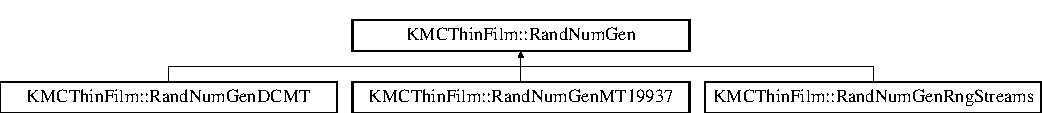
\includegraphics[height=1.523810cm]{classKMCThinFilm_1_1RandNumGen}
\end{center}
\end{figure}
\doxysubsubsection*{Public Member Functions}
\begin{DoxyCompactItemize}
\item 
virtual double \mbox{\hyperlink{classKMCThinFilm_1_1RandNumGen_a3669cf4b6fa2b6acc928bb9ddf24a30a}{get\+Num\+In\+Open\+Interval\+From0\+To1}} ()=0
\end{DoxyCompactItemize}


\doxysubsection{Detailed Description}
Abstract class to implement wrapper classes for random number generators 

\doxysubsection{Member Function Documentation}
\Hypertarget{classKMCThinFilm_1_1RandNumGen_a3669cf4b6fa2b6acc928bb9ddf24a30a}\index{KMCThinFilm::RandNumGen@{KMCThinFilm::RandNumGen}!getNumInOpenIntervalFrom0To1@{getNumInOpenIntervalFrom0To1}}
\index{getNumInOpenIntervalFrom0To1@{getNumInOpenIntervalFrom0To1}!KMCThinFilm::RandNumGen@{KMCThinFilm::RandNumGen}}
\doxysubsubsection{\texorpdfstring{getNumInOpenIntervalFrom0To1()}{getNumInOpenIntervalFrom0To1()}}
{\footnotesize\ttfamily \label{classKMCThinFilm_1_1RandNumGen_a3669cf4b6fa2b6acc928bb9ddf24a30a} 
virtual double KMCThin\+Film\+::\+Rand\+Num\+Gen\+::get\+Num\+In\+Open\+Interval\+From0\+To1 (\begin{DoxyParamCaption}{}{}\end{DoxyParamCaption})\hspace{0.3cm}{\ttfamily [pure virtual]}}

Returns a (pseudo)random number between 0 and 1, {\bfseries{NOT}} including either 0 or 1.

It is especially important for implementations of this class to exclude 0 from this function\textquotesingle{}s return value. The amount of time by which a sector\textquotesingle{}s clock is incremented is proportional to log(r), where r is the return value of the function, and of course, log(0) is undefined.

It is also ill-\/adviced to allow 1 to be a return value of this function, either, since log(1) = 0, which would imply that an event in a KMC simulation took no time at all. 

Implemented in \mbox{\hyperlink{classKMCThinFilm_1_1RandNumGenDCMT_a372003214275ad9889895ff3fabab8d3}{KMCThin\+Film\+::\+Rand\+Num\+Gen\+DCMT}}, \mbox{\hyperlink{classKMCThinFilm_1_1RandNumGenMT19937_abff0a620f02f3e42519697f10f0fedfa}{KMCThin\+Film\+::\+Rand\+Num\+Gen\+MT19937}}, and \mbox{\hyperlink{classKMCThinFilm_1_1RandNumGenRngStreams_ab90d8fff5e0a69f029dc9b6b38bfc64d}{KMCThin\+Film\+::\+Rand\+Num\+Gen\+Rng\+Streams}}.


\doxysection{KMCThin\+Film\+::Rand\+Num\+Gen\+DCMT Class Reference}
\hypertarget{classKMCThinFilm_1_1RandNumGenDCMT}{}\label{classKMCThinFilm_1_1RandNumGenDCMT}\index{KMCThinFilm::RandNumGenDCMT@{KMCThinFilm::RandNumGenDCMT}}


{\ttfamily \#include $<$Rand\+Num\+Gen\+DCMT.\+hpp$>$}

Inheritance diagram for KMCThin\+Film\+::Rand\+Num\+Gen\+DCMT\+:\begin{figure}[H]
\begin{center}
\leavevmode
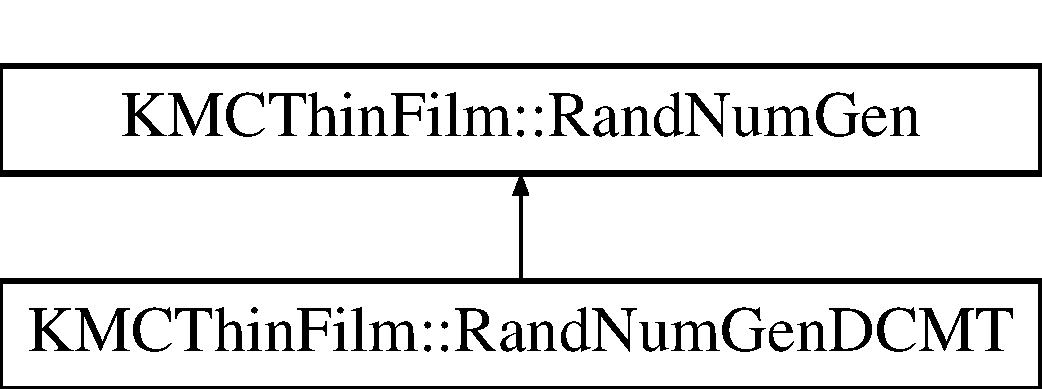
\includegraphics[height=2.000000cm]{classKMCThinFilm_1_1RandNumGenDCMT}
\end{center}
\end{figure}
\doxysubsubsection*{Public Types}
\begin{DoxyCompactItemize}
\item 
enum \mbox{\hyperlink{classKMCThinFilm_1_1RandNumGenDCMT_a8b382ccad8268352985cc35e298296fd}{Period}} \{ \newline
{\bfseries P521} = 521
, {\bfseries P607} = 607
, {\bfseries P1279} = 1279
, {\bfseries P2203} = 2203
, \newline
{\bfseries P2281} = 2281
, {\bfseries P3217} = 3217
, {\bfseries P4253} = 4253
, {\bfseries P4423} = 4423
, \newline
{\bfseries P9689} = 9689
, {\bfseries P9941} = 9941
, {\bfseries P11213} = 11213
, {\bfseries P19937} = 19937
, \newline
{\bfseries P21701} = 21701
, {\bfseries P23209} = 23209
, {\bfseries P44497} = 44497
 \}
\end{DoxyCompactItemize}
\doxysubsubsection*{Public Member Functions}
\begin{DoxyCompactItemize}
\item 
\mbox{\hyperlink{classKMCThinFilm_1_1RandNumGenDCMT_aaba0c646a32c0741e141309ae0cd1422}{Rand\+Num\+Gen\+DCMT}} (int rank, uint32\+\_\+t seed, uint32\+\_\+t seed\+\_\+per\+Proc, \mbox{\hyperlink{classKMCThinFilm_1_1RandNumGenDCMT_a8b382ccad8268352985cc35e298296fd}{Period}} period=P521)
\item 
virtual double \mbox{\hyperlink{classKMCThinFilm_1_1RandNumGenDCMT_a372003214275ad9889895ff3fabab8d3}{get\+Num\+In\+Open\+Interval\+From0\+To1}} ()
\end{DoxyCompactItemize}


\doxysubsection{Detailed Description}
Wrapper class for the parallel pseudorandom number generator library DCMT\+: "{}\+Dynamic Creator of Mersenne Twisters."{}

DCMT is a parallel pseudorandom number generator by Makoto Matsumoto and Takuji Nishimura, and it is based on the serial Mersenne Twister pseudorandom number generator. The library may be obtained from this web page\+: \href{http://www.math.sci.hiroshima-u.ac.jp/~m-mat/MT/DC/dc.html}{\texttt{ http\+://www.\+math.\+sci.\+hiroshima-\/u.\+ac.\+jp/\texorpdfstring{$\sim$}{\string~}m-\/mat/\+MT/\+DC/dc.\+html}} \begin{Desc}
\item[Examples]\par
\mbox{\hyperlink{testFractal_parallel_2testFractal_8cpp-example}{test\+Fractal\+\_\+parallel/test\+Fractal.\+cpp}}.\end{Desc}


\doxysubsection{Member Enumeration Documentation}
\Hypertarget{classKMCThinFilm_1_1RandNumGenDCMT_a8b382ccad8268352985cc35e298296fd}\index{KMCThinFilm::RandNumGenDCMT@{KMCThinFilm::RandNumGenDCMT}!Period@{Period}}
\index{Period@{Period}!KMCThinFilm::RandNumGenDCMT@{KMCThinFilm::RandNumGenDCMT}}
\doxysubsubsection{\texorpdfstring{Period}{Period}}
{\footnotesize\ttfamily \label{classKMCThinFilm_1_1RandNumGenDCMT_a8b382ccad8268352985cc35e298296fd} 
enum \mbox{\hyperlink{classKMCThinFilm_1_1RandNumGenDCMT_a8b382ccad8268352985cc35e298296fd}{KMCThin\+Film\+::\+Rand\+Num\+Gen\+DCMT\+::\+Period}}}

This enumeration forces the {\itshape period} argument of the \doxylink{classKMCThinFilm_1_1RandNumGenDCMT}{Rand\+Num\+Gen\+DCMT} constructor to be one of a certain number of discrete values.

When the value of this enumeration is P{\itshape n}, where {\itshape n} is a number, then the period of the pseudorandom number stream is $2^n - 1$. The value of {\itshape n} is such that the period is a Mersenne prime. 

\doxysubsection{Constructor \& Destructor Documentation}
\Hypertarget{classKMCThinFilm_1_1RandNumGenDCMT_aaba0c646a32c0741e141309ae0cd1422}\index{KMCThinFilm::RandNumGenDCMT@{KMCThinFilm::RandNumGenDCMT}!RandNumGenDCMT@{RandNumGenDCMT}}
\index{RandNumGenDCMT@{RandNumGenDCMT}!KMCThinFilm::RandNumGenDCMT@{KMCThinFilm::RandNumGenDCMT}}
\doxysubsubsection{\texorpdfstring{RandNumGenDCMT()}{RandNumGenDCMT()}}
{\footnotesize\ttfamily \label{classKMCThinFilm_1_1RandNumGenDCMT_aaba0c646a32c0741e141309ae0cd1422} 
KMCThin\+Film\+::\+Rand\+Num\+Gen\+DCMT\+::\+Rand\+Num\+Gen\+DCMT (\begin{DoxyParamCaption}\item[{int}]{rank}{, }\item[{uint32\+\_\+t}]{seed}{, }\item[{uint32\+\_\+t}]{seed\+\_\+per\+Proc}{, }\item[{\mbox{\hyperlink{classKMCThinFilm_1_1RandNumGenDCMT_a8b382ccad8268352985cc35e298296fd}{Period}}}]{period}{ = {\ttfamily P521}}\end{DoxyParamCaption})}

Constructor, sets the initial state for each of the parallel streams of the pseudorandom number generator. 
\begin{DoxyParams}{Parameters}
{\em rank} & MPI rank of the processor  \\
\hline
{\em seed} & Global seed for the pseudorandom number generator  \\
\hline
{\em seed\+\_\+per\+Proc} & Per-\/processor seed for the pseudorandom number generator, should be different for each process  \\
\hline
{\em period} & Enumeration constant indicating the exponent for the period of the pseudorandom number stream \\
\hline
\end{DoxyParams}


\doxysubsection{Member Function Documentation}
\Hypertarget{classKMCThinFilm_1_1RandNumGenDCMT_a372003214275ad9889895ff3fabab8d3}\index{KMCThinFilm::RandNumGenDCMT@{KMCThinFilm::RandNumGenDCMT}!getNumInOpenIntervalFrom0To1@{getNumInOpenIntervalFrom0To1}}
\index{getNumInOpenIntervalFrom0To1@{getNumInOpenIntervalFrom0To1}!KMCThinFilm::RandNumGenDCMT@{KMCThinFilm::RandNumGenDCMT}}
\doxysubsubsection{\texorpdfstring{getNumInOpenIntervalFrom0To1()}{getNumInOpenIntervalFrom0To1()}}
{\footnotesize\ttfamily \label{classKMCThinFilm_1_1RandNumGenDCMT_a372003214275ad9889895ff3fabab8d3} 
virtual double KMCThin\+Film\+::\+Rand\+Num\+Gen\+DCMT\+::get\+Num\+In\+Open\+Interval\+From0\+To1 (\begin{DoxyParamCaption}{}{}\end{DoxyParamCaption})\hspace{0.3cm}{\ttfamily [virtual]}}

Returns a (pseudo)random number between 0 and 1, not including either 0 or 1. 

Implements \mbox{\hyperlink{classKMCThinFilm_1_1RandNumGen_a3669cf4b6fa2b6acc928bb9ddf24a30a}{KMCThin\+Film\+::\+Rand\+Num\+Gen}}.


\doxysection{KMCThin\+Film\+::Rand\+Num\+Gen\+MT19937 Class Reference}
\hypertarget{classKMCThinFilm_1_1RandNumGenMT19937}{}\label{classKMCThinFilm_1_1RandNumGenMT19937}\index{KMCThinFilm::RandNumGenMT19937@{KMCThinFilm::RandNumGenMT19937}}


{\ttfamily \#include $<$Rand\+Num\+Gen\+MT19937.\+hpp$>$}

Inheritance diagram for KMCThin\+Film\+::Rand\+Num\+Gen\+MT19937\+:\begin{figure}[H]
\begin{center}
\leavevmode
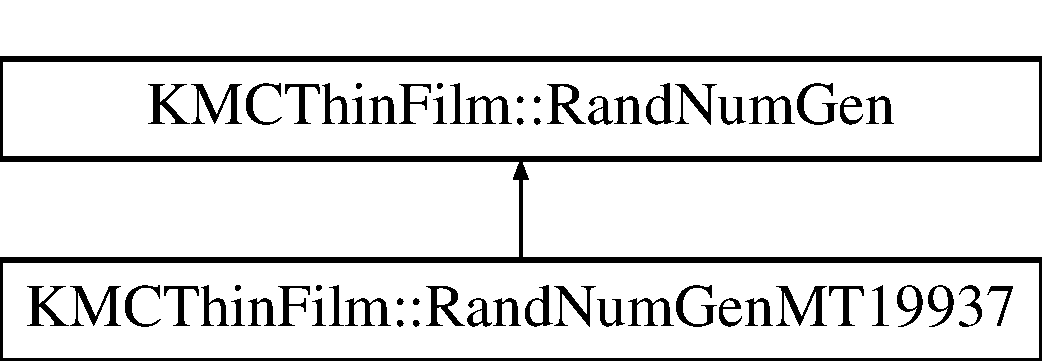
\includegraphics[height=2.000000cm]{classKMCThinFilm_1_1RandNumGenMT19937}
\end{center}
\end{figure}
\doxysubsubsection*{Public Member Functions}
\begin{DoxyCompactItemize}
\item 
\mbox{\hyperlink{classKMCThinFilm_1_1RandNumGenMT19937_af6aa949c0c59271fb9c3ddae309312ac}{Rand\+Num\+Gen\+MT19937}} (unsigned int seed)
\item 
virtual double \mbox{\hyperlink{classKMCThinFilm_1_1RandNumGenMT19937_abff0a620f02f3e42519697f10f0fedfa}{get\+Num\+In\+Open\+Interval\+From0\+To1}} ()
\end{DoxyCompactItemize}


\doxysubsection{Detailed Description}
Wrapper class for the {\itshape serial} Mersenne Twister pseudorandom number generator with a period of $2^{19937} - 1$.

This is not recommended for parallel simulations. \begin{Desc}
\item[Examples]\par
\mbox{\hyperlink{testBallisticDep1_2testBallisticDep_8cpp-example}{test\+Ballistic\+Dep1/test\+Ballistic\+Dep.\+cpp}}, \mbox{\hyperlink{testBallisticDep2_2testBallisticDep_8cpp-example}{test\+Ballistic\+Dep2/test\+Ballistic\+Dep.\+cpp}}, \mbox{\hyperlink{testFractal_2testFractal_8cpp-example}{test\+Fractal/test\+Fractal.\+cpp}}, \mbox{\hyperlink{testFractal_parallel_2testFractal_8cpp-example}{test\+Fractal\+\_\+parallel/test\+Fractal.\+cpp}}, \mbox{\hyperlink{testFractal_semi_manual_track_2testFractal_8cpp-example}{test\+Fractal\+\_\+semi\+\_\+manual\+\_\+track/test\+Fractal.\+cpp}}, \mbox{\hyperlink{testPatternedSurface1_2testPatternedSurface_8cpp-example}{test\+Patterned\+Surface1/test\+Patterned\+Surface.\+cpp}}, and \mbox{\hyperlink{testPatternedSurface2_2testPatternedSurface_8cpp-example}{test\+Patterned\+Surface2/test\+Patterned\+Surface.\+cpp}}.\end{Desc}


\doxysubsection{Constructor \& Destructor Documentation}
\Hypertarget{classKMCThinFilm_1_1RandNumGenMT19937_af6aa949c0c59271fb9c3ddae309312ac}\index{KMCThinFilm::RandNumGenMT19937@{KMCThinFilm::RandNumGenMT19937}!RandNumGenMT19937@{RandNumGenMT19937}}
\index{RandNumGenMT19937@{RandNumGenMT19937}!KMCThinFilm::RandNumGenMT19937@{KMCThinFilm::RandNumGenMT19937}}
\doxysubsubsection{\texorpdfstring{RandNumGenMT19937()}{RandNumGenMT19937()}}
{\footnotesize\ttfamily \label{classKMCThinFilm_1_1RandNumGenMT19937_af6aa949c0c59271fb9c3ddae309312ac} 
KMCThin\+Film\+::\+Rand\+Num\+Gen\+MT19937\+::\+Rand\+Num\+Gen\+MT19937 (\begin{DoxyParamCaption}\item[{unsigned int}]{seed}{}\end{DoxyParamCaption})\hspace{0.3cm}{\ttfamily [inline]}}

Constructor, sets the initial state for the pseudorandom number generator. 

\doxysubsection{Member Function Documentation}
\Hypertarget{classKMCThinFilm_1_1RandNumGenMT19937_abff0a620f02f3e42519697f10f0fedfa}\index{KMCThinFilm::RandNumGenMT19937@{KMCThinFilm::RandNumGenMT19937}!getNumInOpenIntervalFrom0To1@{getNumInOpenIntervalFrom0To1}}
\index{getNumInOpenIntervalFrom0To1@{getNumInOpenIntervalFrom0To1}!KMCThinFilm::RandNumGenMT19937@{KMCThinFilm::RandNumGenMT19937}}
\doxysubsubsection{\texorpdfstring{getNumInOpenIntervalFrom0To1()}{getNumInOpenIntervalFrom0To1()}}
{\footnotesize\ttfamily \label{classKMCThinFilm_1_1RandNumGenMT19937_abff0a620f02f3e42519697f10f0fedfa} 
virtual double KMCThin\+Film\+::\+Rand\+Num\+Gen\+MT19937\+::get\+Num\+In\+Open\+Interval\+From0\+To1 (\begin{DoxyParamCaption}{}{}\end{DoxyParamCaption})\hspace{0.3cm}{\ttfamily [virtual]}}

Returns a (pseudo)random number between 0 and 1, not including either 0 or 1. 

Implements \mbox{\hyperlink{classKMCThinFilm_1_1RandNumGen_a3669cf4b6fa2b6acc928bb9ddf24a30a}{KMCThin\+Film\+::\+Rand\+Num\+Gen}}.


\doxysection{KMCThin\+Film\+::Rand\+Num\+Gen\+Rng\+Streams Class Reference}
\hypertarget{classKMCThinFilm_1_1RandNumGenRngStreams}{}\label{classKMCThinFilm_1_1RandNumGenRngStreams}\index{KMCThinFilm::RandNumGenRngStreams@{KMCThinFilm::RandNumGenRngStreams}}


{\ttfamily \#include $<$Rand\+Num\+Gen\+Rng\+Streams.\+hpp$>$}

Inheritance diagram for KMCThin\+Film\+::Rand\+Num\+Gen\+Rng\+Streams\+:\begin{figure}[H]
\begin{center}
\leavevmode
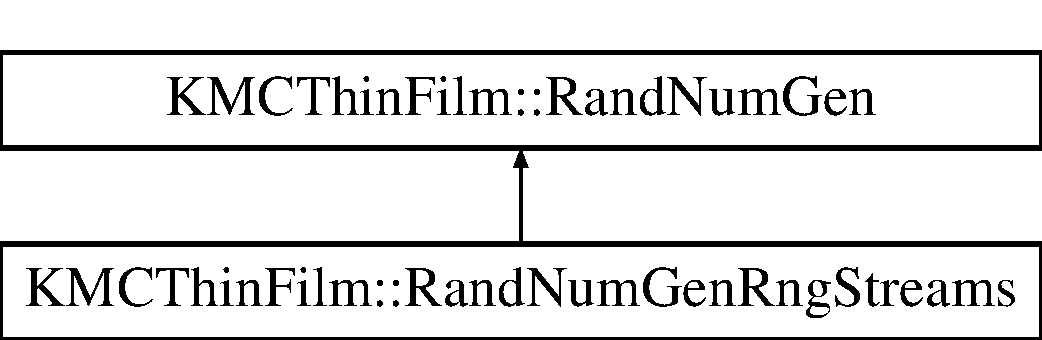
\includegraphics[height=2.000000cm]{classKMCThinFilm_1_1RandNumGenRngStreams}
\end{center}
\end{figure}
\doxysubsubsection*{Public Member Functions}
\begin{DoxyCompactItemize}
\item 
\mbox{\hyperlink{classKMCThinFilm_1_1RandNumGenRngStreams_abeb90e642db294c0a846009fdc099913}{Rand\+Num\+Gen\+Rng\+Streams}} (std\+::vector$<$ unsigned long $>$ \&seed, int rank, long adv\+Exp=127, long adv\+Const=0)
\item 
virtual double \mbox{\hyperlink{classKMCThinFilm_1_1RandNumGenRngStreams_ab90d8fff5e0a69f029dc9b6b38bfc64d}{get\+Num\+In\+Open\+Interval\+From0\+To1}} ()
\end{DoxyCompactItemize}


\doxysubsection{Detailed Description}
Wrapper class for the parallel pseudorandom number generator library Rng\+Streams.

Rng\+Streams is a parallel pseudorandom number generator by Pierre L\textquotesingle{}Ecuyer and Richard Simard. It may be obtained from this web page\+: \href{http://statmath.wu.ac.at/software/RngStreams/}{\texttt{ http\+://statmath.\+wu.\+ac.\+at/software/\+Rng\+Streams/}} 

\doxysubsection{Constructor \& Destructor Documentation}
\Hypertarget{classKMCThinFilm_1_1RandNumGenRngStreams_abeb90e642db294c0a846009fdc099913}\index{KMCThinFilm::RandNumGenRngStreams@{KMCThinFilm::RandNumGenRngStreams}!RandNumGenRngStreams@{RandNumGenRngStreams}}
\index{RandNumGenRngStreams@{RandNumGenRngStreams}!KMCThinFilm::RandNumGenRngStreams@{KMCThinFilm::RandNumGenRngStreams}}
\doxysubsubsection{\texorpdfstring{RandNumGenRngStreams()}{RandNumGenRngStreams()}}
{\footnotesize\ttfamily \label{classKMCThinFilm_1_1RandNumGenRngStreams_abeb90e642db294c0a846009fdc099913} 
KMCThin\+Film\+::\+Rand\+Num\+Gen\+Rng\+Streams\+::\+Rand\+Num\+Gen\+Rng\+Streams (\begin{DoxyParamCaption}\item[{std\+::vector$<$ unsigned long $>$ \&}]{seed}{, }\item[{int}]{rank}{, }\item[{long}]{adv\+Exp}{ = {\ttfamily 127}, }\item[{long}]{adv\+Const}{ = {\ttfamily 0}}\end{DoxyParamCaption})}

Constructor, sets the initial state for each of the parallel streams of the pseudorandom number generator.

The vector {\itshape seed} that seeds the pseudorandom number generator must have a length of 6, and it should be the same for every process.

Each parallel pseudorandom number stream is offset by  $rank
\times (2^{advExp} + advConst)$, if {\itshape adv\+Exp} is nonnegative, or $rank \times (-2^{-advExp} + advConst)$, otherwise. The argument {\itshape rank} should be the MPI rank of the processor. 

\doxysubsection{Member Function Documentation}
\Hypertarget{classKMCThinFilm_1_1RandNumGenRngStreams_ab90d8fff5e0a69f029dc9b6b38bfc64d}\index{KMCThinFilm::RandNumGenRngStreams@{KMCThinFilm::RandNumGenRngStreams}!getNumInOpenIntervalFrom0To1@{getNumInOpenIntervalFrom0To1}}
\index{getNumInOpenIntervalFrom0To1@{getNumInOpenIntervalFrom0To1}!KMCThinFilm::RandNumGenRngStreams@{KMCThinFilm::RandNumGenRngStreams}}
\doxysubsubsection{\texorpdfstring{getNumInOpenIntervalFrom0To1()}{getNumInOpenIntervalFrom0To1()}}
{\footnotesize\ttfamily \label{classKMCThinFilm_1_1RandNumGenRngStreams_ab90d8fff5e0a69f029dc9b6b38bfc64d} 
virtual double KMCThin\+Film\+::\+Rand\+Num\+Gen\+Rng\+Streams\+::get\+Num\+In\+Open\+Interval\+From0\+To1 (\begin{DoxyParamCaption}{}{}\end{DoxyParamCaption})\hspace{0.3cm}{\ttfamily [virtual]}}

Returns a (pseudo)random number between 0 and 1, not including either 0 or 1. 

Implements \mbox{\hyperlink{classKMCThinFilm_1_1RandNumGen_a3669cf4b6fa2b6acc928bb9ddf24a30a}{KMCThin\+Film\+::\+Rand\+Num\+Gen}}.


\doxysection{KMCThin\+Film\+::Time\+Incr\+::Scheme\+Vars Class Reference}
\hypertarget{classKMCThinFilm_1_1TimeIncr_1_1SchemeVars}{}\label{classKMCThinFilm_1_1TimeIncr_1_1SchemeVars}\index{KMCThinFilm::TimeIncr::SchemeVars@{KMCThinFilm::TimeIncr::SchemeVars}}


{\ttfamily \#include $<$Time\+Incr\+Scheme\+Vars.\+hpp$>$}

\doxysubsubsection*{Public Member Functions}
\begin{DoxyCompactItemize}
\item 
\mbox{\hyperlink{namespaceKMCThinFilm_1_1TimeIncr_1_1SchemeName_a9d8be73a26298e6c4379c28285902534}{Scheme\+Name\+::\+Type}} \mbox{\hyperlink{classKMCThinFilm_1_1TimeIncr_1_1SchemeVars_a8a6b278ab771b3ca06ce8c5478ebec94}{get\+Scheme\+Name}} () const
\item 
double \mbox{\hyperlink{classKMCThinFilm_1_1TimeIncr_1_1SchemeVars_a74523fbff49d74027dff1532d500155d}{get\+Scheme\+Param\+If\+Available}} (\mbox{\hyperlink{namespaceKMCThinFilm_1_1TimeIncr_1_1SchemeParam_a1ee2f5f6234ea51c6d8ae6993aee48ca}{Scheme\+Param\+::\+Type}} param\+Name, bool \&is\+Available) const
\item 
double \mbox{\hyperlink{classKMCThinFilm_1_1TimeIncr_1_1SchemeVars_a935e8443003476cefda9e4b06416032d}{get\+Scheme\+Param\+Or\+Die}} (\mbox{\hyperlink{namespaceKMCThinFilm_1_1TimeIncr_1_1SchemeParam_a1ee2f5f6234ea51c6d8ae6993aee48ca}{Scheme\+Param\+::\+Type}} param\+Name, const std\+::string \&msg\+If\+Die) const
\item 
double \mbox{\hyperlink{classKMCThinFilm_1_1TimeIncr_1_1SchemeVars_a25605a924e6301a9ac472ebd0c37d370}{get\+Scheme\+Param\+Or\+Return\+Default\+Val}} (\mbox{\hyperlink{namespaceKMCThinFilm_1_1TimeIncr_1_1SchemeParam_a1ee2f5f6234ea51c6d8ae6993aee48ca}{Scheme\+Param\+::\+Type}} param\+Name, double default\+Val) const
\item 
void \mbox{\hyperlink{classKMCThinFilm_1_1TimeIncr_1_1SchemeVars_a9c534dc3967fe996205a22d3b4eb9efc}{set\+Scheme\+Name}} (\mbox{\hyperlink{namespaceKMCThinFilm_1_1TimeIncr_1_1SchemeName_a9d8be73a26298e6c4379c28285902534}{Scheme\+Name\+::\+Type}} name)
\item 
void \mbox{\hyperlink{classKMCThinFilm_1_1TimeIncr_1_1SchemeVars_a791374d98d976927c656d4adabe19f8d}{set\+Scheme\+Param}} (\mbox{\hyperlink{namespaceKMCThinFilm_1_1TimeIncr_1_1SchemeParam_a1ee2f5f6234ea51c6d8ae6993aee48ca}{Scheme\+Param\+::\+Type}} param\+Name, double param\+Val)
\end{DoxyCompactItemize}


\doxysubsection{Detailed Description}
Type of object used to store parameters for the parallel time stepping schemes.

Note that in a typical use of a class instance of this, the set\texorpdfstring{$\ast$}{*}() functions will tend to be used rather than the get\texorpdfstring{$\ast$}{*}() functions. However, the get\texorpdfstring{$\ast$}{*}() functions are exposed for the sake of testing and debugging. \begin{Desc}
\item[Examples]\par
\mbox{\hyperlink{testFractal_parallel_2testFractal_8cpp-example}{test\+Fractal\+\_\+parallel/test\+Fractal.\+cpp}}.\end{Desc}


\doxysubsection{Member Function Documentation}
\Hypertarget{classKMCThinFilm_1_1TimeIncr_1_1SchemeVars_a8a6b278ab771b3ca06ce8c5478ebec94}\index{KMCThinFilm::TimeIncr::SchemeVars@{KMCThinFilm::TimeIncr::SchemeVars}!getSchemeName@{getSchemeName}}
\index{getSchemeName@{getSchemeName}!KMCThinFilm::TimeIncr::SchemeVars@{KMCThinFilm::TimeIncr::SchemeVars}}
\doxysubsubsection{\texorpdfstring{getSchemeName()}{getSchemeName()}}
{\footnotesize\ttfamily \label{classKMCThinFilm_1_1TimeIncr_1_1SchemeVars_a8a6b278ab771b3ca06ce8c5478ebec94} 
\mbox{\hyperlink{namespaceKMCThinFilm_1_1TimeIncr_1_1SchemeName_a9d8be73a26298e6c4379c28285902534}{Scheme\+Name\+::\+Type}} KMCThin\+Film\+::\+Time\+Incr\+::\+Scheme\+Vars\+::get\+Scheme\+Name (\begin{DoxyParamCaption}{}{}\end{DoxyParamCaption}) const}

Returns the name of the time-\/stepping scheme set by \doxylink{classKMCThinFilm_1_1TimeIncr_1_1SchemeVars_a9c534dc3967fe996205a22d3b4eb9efc}{set\+Scheme\+Name()}. \Hypertarget{classKMCThinFilm_1_1TimeIncr_1_1SchemeVars_a74523fbff49d74027dff1532d500155d}\index{KMCThinFilm::TimeIncr::SchemeVars@{KMCThinFilm::TimeIncr::SchemeVars}!getSchemeParamIfAvailable@{getSchemeParamIfAvailable}}
\index{getSchemeParamIfAvailable@{getSchemeParamIfAvailable}!KMCThinFilm::TimeIncr::SchemeVars@{KMCThinFilm::TimeIncr::SchemeVars}}
\doxysubsubsection{\texorpdfstring{getSchemeParamIfAvailable()}{getSchemeParamIfAvailable()}}
{\footnotesize\ttfamily \label{classKMCThinFilm_1_1TimeIncr_1_1SchemeVars_a74523fbff49d74027dff1532d500155d} 
double KMCThin\+Film\+::\+Time\+Incr\+::\+Scheme\+Vars\+::get\+Scheme\+Param\+If\+Available (\begin{DoxyParamCaption}\item[{\mbox{\hyperlink{namespaceKMCThinFilm_1_1TimeIncr_1_1SchemeParam_a1ee2f5f6234ea51c6d8ae6993aee48ca}{Scheme\+Param\+::\+Type}}}]{param\+Name}{, }\item[{bool \&}]{is\+Available}{}\end{DoxyParamCaption}) const}

Returns the value of the parameter, if it has been set.

It is not an error if the parameter was not set, but if it wasn\textquotesingle{}t, then the return value is likely garbage. 
\begin{DoxyParams}{Parameters}
{\em param\+Name} & Name of parameter  \\
\hline
{\em is\+Available} & If this is false, then the parameter was not set. \\
\hline
\end{DoxyParams}
\Hypertarget{classKMCThinFilm_1_1TimeIncr_1_1SchemeVars_a935e8443003476cefda9e4b06416032d}\index{KMCThinFilm::TimeIncr::SchemeVars@{KMCThinFilm::TimeIncr::SchemeVars}!getSchemeParamOrDie@{getSchemeParamOrDie}}
\index{getSchemeParamOrDie@{getSchemeParamOrDie}!KMCThinFilm::TimeIncr::SchemeVars@{KMCThinFilm::TimeIncr::SchemeVars}}
\doxysubsubsection{\texorpdfstring{getSchemeParamOrDie()}{getSchemeParamOrDie()}}
{\footnotesize\ttfamily \label{classKMCThinFilm_1_1TimeIncr_1_1SchemeVars_a935e8443003476cefda9e4b06416032d} 
double KMCThin\+Film\+::\+Time\+Incr\+::\+Scheme\+Vars\+::get\+Scheme\+Param\+Or\+Die (\begin{DoxyParamCaption}\item[{\mbox{\hyperlink{namespaceKMCThinFilm_1_1TimeIncr_1_1SchemeParam_a1ee2f5f6234ea51c6d8ae6993aee48ca}{Scheme\+Param\+::\+Type}}}]{param\+Name}{, }\item[{const std\+::string \&}]{msg\+If\+Die}{}\end{DoxyParamCaption}) const}

Returns the value of the parameter or causes the KMC application to terminate with an error message. 
\begin{DoxyParams}{Parameters}
{\em param\+Name} & Name of parameter  \\
\hline
{\em msg\+If\+Die} & Error message printed if the parameter was not set. \\
\hline
\end{DoxyParams}
\Hypertarget{classKMCThinFilm_1_1TimeIncr_1_1SchemeVars_a25605a924e6301a9ac472ebd0c37d370}\index{KMCThinFilm::TimeIncr::SchemeVars@{KMCThinFilm::TimeIncr::SchemeVars}!getSchemeParamOrReturnDefaultVal@{getSchemeParamOrReturnDefaultVal}}
\index{getSchemeParamOrReturnDefaultVal@{getSchemeParamOrReturnDefaultVal}!KMCThinFilm::TimeIncr::SchemeVars@{KMCThinFilm::TimeIncr::SchemeVars}}
\doxysubsubsection{\texorpdfstring{getSchemeParamOrReturnDefaultVal()}{getSchemeParamOrReturnDefaultVal()}}
{\footnotesize\ttfamily \label{classKMCThinFilm_1_1TimeIncr_1_1SchemeVars_a25605a924e6301a9ac472ebd0c37d370} 
double KMCThin\+Film\+::\+Time\+Incr\+::\+Scheme\+Vars\+::get\+Scheme\+Param\+Or\+Return\+Default\+Val (\begin{DoxyParamCaption}\item[{\mbox{\hyperlink{namespaceKMCThinFilm_1_1TimeIncr_1_1SchemeParam_a1ee2f5f6234ea51c6d8ae6993aee48ca}{Scheme\+Param\+::\+Type}}}]{param\+Name}{, }\item[{double}]{default\+Val}{}\end{DoxyParamCaption}) const}

Returns the value of the parameter if it has been set, and returns a default value otherwise. 
\begin{DoxyParams}{Parameters}
{\em param\+Name} & Name of parameter  \\
\hline
{\em default\+Val} & The value to be returned if the parameter was not set. \\
\hline
\end{DoxyParams}
\Hypertarget{classKMCThinFilm_1_1TimeIncr_1_1SchemeVars_a9c534dc3967fe996205a22d3b4eb9efc}\index{KMCThinFilm::TimeIncr::SchemeVars@{KMCThinFilm::TimeIncr::SchemeVars}!setSchemeName@{setSchemeName}}
\index{setSchemeName@{setSchemeName}!KMCThinFilm::TimeIncr::SchemeVars@{KMCThinFilm::TimeIncr::SchemeVars}}
\doxysubsubsection{\texorpdfstring{setSchemeName()}{setSchemeName()}}
{\footnotesize\ttfamily \label{classKMCThinFilm_1_1TimeIncr_1_1SchemeVars_a9c534dc3967fe996205a22d3b4eb9efc} 
void KMCThin\+Film\+::\+Time\+Incr\+::\+Scheme\+Vars\+::set\+Scheme\+Name (\begin{DoxyParamCaption}\item[{\mbox{\hyperlink{namespaceKMCThinFilm_1_1TimeIncr_1_1SchemeName_a9d8be73a26298e6c4379c28285902534}{Scheme\+Name\+::\+Type}}}]{name}{}\end{DoxyParamCaption})}

Sets the name of the time-\/stepping scheme to be used. \begin{Desc}
\item[Examples]\par
\mbox{\hyperlink{testFractal_parallel_2testFractal_8cpp-example}{test\+Fractal\+\_\+parallel/test\+Fractal.\+cpp}}.\end{Desc}
\Hypertarget{classKMCThinFilm_1_1TimeIncr_1_1SchemeVars_a791374d98d976927c656d4adabe19f8d}\index{KMCThinFilm::TimeIncr::SchemeVars@{KMCThinFilm::TimeIncr::SchemeVars}!setSchemeParam@{setSchemeParam}}
\index{setSchemeParam@{setSchemeParam}!KMCThinFilm::TimeIncr::SchemeVars@{KMCThinFilm::TimeIncr::SchemeVars}}
\doxysubsubsection{\texorpdfstring{setSchemeParam()}{setSchemeParam()}}
{\footnotesize\ttfamily \label{classKMCThinFilm_1_1TimeIncr_1_1SchemeVars_a791374d98d976927c656d4adabe19f8d} 
void KMCThin\+Film\+::\+Time\+Incr\+::\+Scheme\+Vars\+::set\+Scheme\+Param (\begin{DoxyParamCaption}\item[{\mbox{\hyperlink{namespaceKMCThinFilm_1_1TimeIncr_1_1SchemeParam_a1ee2f5f6234ea51c6d8ae6993aee48ca}{Scheme\+Param\+::\+Type}}}]{param\+Name}{, }\item[{double}]{param\+Val}{}\end{DoxyParamCaption})}

Sets a parameter of the time-\/stepping scheme to be used. 
\begin{DoxyParams}{Parameters}
{\em param\+Name} & Name of parameter  \\
\hline
{\em param\+Val} & Value of parameter \\
\hline
\end{DoxyParams}
\begin{Desc}
\item[Examples]\par
\mbox{\hyperlink{testFractal_parallel_2testFractal_8cpp-example}{test\+Fractal\+\_\+parallel/test\+Fractal.\+cpp}}.\end{Desc}

\doxysection{KMCThin\+Film\+::Simulation Class Reference}
\hypertarget{classKMCThinFilm_1_1Simulation}{}\label{classKMCThinFilm_1_1Simulation}\index{KMCThinFilm::Simulation@{KMCThinFilm::Simulation}}


{\ttfamily \#include $<$Simulation.\+hpp$>$}

Inheritance diagram for KMCThin\+Film\+::Simulation\+:\begin{figure}[H]
\begin{center}
\leavevmode
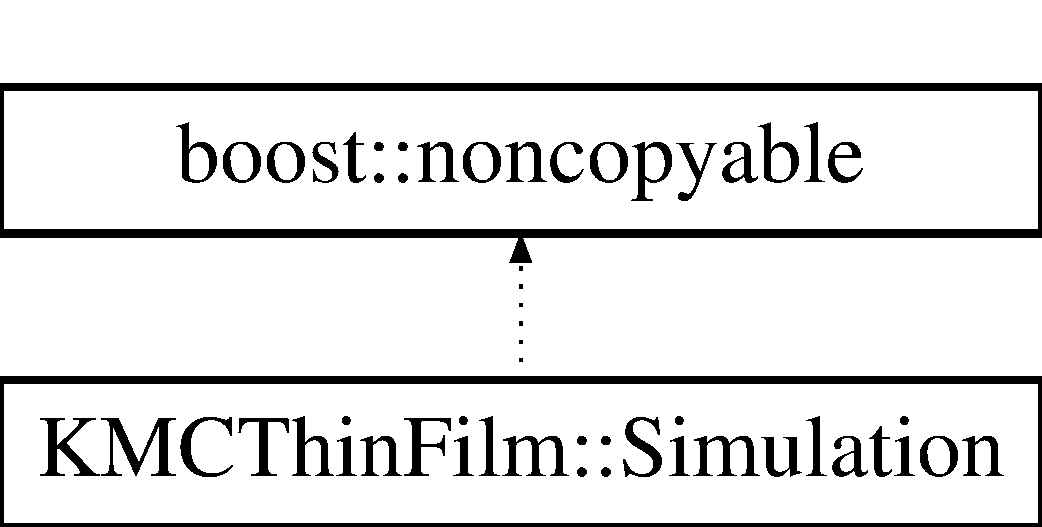
\includegraphics[height=2.000000cm]{classKMCThinFilm_1_1Simulation}
\end{center}
\end{figure}
\doxysubsubsection*{Public Member Functions}
\begin{DoxyCompactItemize}
\item 
\mbox{\hyperlink{classKMCThinFilm_1_1Simulation_ac5a1023e231685fda3a421e86beff980}{Simulation}} (const \mbox{\hyperlink{structKMCThinFilm_1_1LatticeParams}{Lattice\+Params}} \&params\+For\+Lattice)
\item 
void \mbox{\hyperlink{classKMCThinFilm_1_1Simulation_ada268bce065b942617fd1331b083626d}{add\+Cell\+Centered\+Event\+Group}} (int event\+Group\+Id, const \mbox{\hyperlink{classKMCThinFilm_1_1CellNeighOffsets}{Cell\+Neigh\+Offsets}} \&cno, \mbox{\hyperlink{namespaceKMCThinFilm_afc58c6c4948aa7d7243beb0990a563f1}{Cell\+Centered\+Group\+Propensities}} propensities, const \mbox{\hyperlink{classKMCThinFilm_1_1EventExecutorGroup}{Event\+Executor\+Group}} \&event\+Executor\+Group)
\item 
void \mbox{\hyperlink{classKMCThinFilm_1_1Simulation_affa3dff53afd248546457944b98376d9}{add\+Over\+Lattice\+Event}} (int event\+Id, double propensity\+Per\+Unit\+Area, \mbox{\hyperlink{namespaceKMCThinFilm_a601f0f23e6b591202d40f27df34db951}{Event\+Executor\+Auto\+Track}} event\+Executor)
\item 
void \mbox{\hyperlink{classKMCThinFilm_1_1Simulation_a8513218aee1c117ec324b8a9cdef6ccf}{add\+Over\+Lattice\+Event}} (int event\+Id, double propensity\+Per\+Unit\+Area, \mbox{\hyperlink{namespaceKMCThinFilm_a92a9e6c3ced8703f95265e85d80f1797}{Event\+Executor\+Semi\+Manual\+Track}} event\+Executor, const std\+::vector$<$ \mbox{\hyperlink{classKMCThinFilm_1_1CellNeighOffsets}{Cell\+Neigh\+Offsets}} $>$ \&cno\+Vec)
\item 
void \mbox{\hyperlink{classKMCThinFilm_1_1Simulation_a5280f709245a66489eb357f488082528}{add\+Step\+Periodic\+Action}} (int action\+Id, \mbox{\hyperlink{namespaceKMCThinFilm_ab48bbcbabdf454a07e2f0edb47404abe}{Periodic\+Action}} action, int period\+Of\+Steps, bool do\+At\+Sim\+End)
\item 
void \mbox{\hyperlink{classKMCThinFilm_1_1Simulation_a2d0b886ef44d3acf0a8c018a7042e1d9}{add\+Time\+Periodic\+Action}} (int action\+Id, \mbox{\hyperlink{namespaceKMCThinFilm_ab48bbcbabdf454a07e2f0edb47404abe}{Periodic\+Action}} action, double period\+Of\+Time, bool do\+At\+Sim\+End)
\item 
void \mbox{\hyperlink{classKMCThinFilm_1_1Simulation_a4caf800d8630e74210e0301da0238f6a}{change\+Cell\+Centered\+Event\+Group}} (int event\+Group\+Id, const \mbox{\hyperlink{classKMCThinFilm_1_1CellNeighOffsets}{Cell\+Neigh\+Offsets}} \&cno, \mbox{\hyperlink{namespaceKMCThinFilm_afc58c6c4948aa7d7243beb0990a563f1}{Cell\+Centered\+Group\+Propensities}} propensities, const \mbox{\hyperlink{classKMCThinFilm_1_1EventExecutorGroup}{Event\+Executor\+Group}} \&event\+Executor\+Group)
\item 
void \mbox{\hyperlink{classKMCThinFilm_1_1Simulation_a3a45062725c9fe3a70e21200d01bafba}{change\+Over\+Lattice\+Event}} (int event\+Id, double propensity\+Per\+Unit\+Area, \mbox{\hyperlink{namespaceKMCThinFilm_a601f0f23e6b591202d40f27df34db951}{Event\+Executor\+Auto\+Track}} event\+Executor)
\item 
void \mbox{\hyperlink{classKMCThinFilm_1_1Simulation_a1ddc6a10209942546b0e42392a1dbfe8}{change\+Over\+Lattice\+Event}} (int event\+Id, double propensity\+Per\+Unit\+Area, \mbox{\hyperlink{namespaceKMCThinFilm_a92a9e6c3ced8703f95265e85d80f1797}{Event\+Executor\+Semi\+Manual\+Track}} event\+Executor, const std\+::vector$<$ \mbox{\hyperlink{classKMCThinFilm_1_1CellNeighOffsets}{Cell\+Neigh\+Offsets}} $>$ \&cno\+Vec)
\item 
void \mbox{\hyperlink{classKMCThinFilm_1_1Simulation_a529e986f0c320259497e08ac684c89d5}{change\+Step\+Periodic\+Action}} (int action\+Id, \mbox{\hyperlink{namespaceKMCThinFilm_ab48bbcbabdf454a07e2f0edb47404abe}{Periodic\+Action}} action, int period\+Of\+Steps, bool do\+At\+Sim\+End)
\item 
void \mbox{\hyperlink{classKMCThinFilm_1_1Simulation_a2baf3e0cf9ae646f8bc09fc704316bb4}{change\+Time\+Periodic\+Action}} (int action\+Id, \mbox{\hyperlink{namespaceKMCThinFilm_ab48bbcbabdf454a07e2f0edb47404abe}{Periodic\+Action}} action, double period\+Of\+Time, bool do\+At\+Sim\+End)
\item 
const MPI\+\_\+\+Comm \& \mbox{\hyperlink{classKMCThinFilm_1_1Simulation_a7fa4b341178e7b2bb32a598a72035b5b}{comm}} () const
\item 
int \mbox{\hyperlink{classKMCThinFilm_1_1Simulation_ab25825583016491e2df8bbb377e5a59a}{comm\+Coord}} (int dim) const
\item 
double \mbox{\hyperlink{classKMCThinFilm_1_1Simulation_ae70c8f71a13bf376234af627129cc4a4}{elapsed\+Time}} () const
\item 
void \mbox{\hyperlink{classKMCThinFilm_1_1Simulation_ae397f0319a4e978f1d754e7f8bedcd01}{get\+Lattice\+Global\+Planar\+BBox}} (\mbox{\hyperlink{structKMCThinFilm_1_1LatticePlanarBBox}{Lattice\+Planar\+BBox}} \&bbox) const
\item 
void \mbox{\hyperlink{classKMCThinFilm_1_1Simulation_a67278594ebc8ee6be87f153334bd4ab9}{get\+Lattice\+Local\+Planar\+BBox}} (bool w\+Ghost, \mbox{\hyperlink{structKMCThinFilm_1_1LatticePlanarBBox}{Lattice\+Planar\+BBox}} \&bbox) const
\item 
void \mbox{\hyperlink{classKMCThinFilm_1_1Simulation_a1fa737caf023560abb4b862fe581c3de}{get\+Lattice\+Sector\+Planar\+BBox}} (int sect\+Num, \mbox{\hyperlink{structKMCThinFilm_1_1LatticePlanarBBox}{Lattice\+Planar\+BBox}} \&bbox) const
\item 
int \mbox{\hyperlink{classKMCThinFilm_1_1Simulation_ac09e29f5535debb54cd1fe50690dde3d}{n\+Procs}} () const
\item 
unsigned long long \mbox{\hyperlink{classKMCThinFilm_1_1Simulation_ac9436832964b46d46978671664445584}{num\+Global\+Steps}} () const
\item 
unsigned long long \mbox{\hyperlink{classKMCThinFilm_1_1Simulation_a5a722b36af5090fa2b397ad3bebf70e4}{num\+Local\+Events}} () const
\item 
int \mbox{\hyperlink{classKMCThinFilm_1_1Simulation_a4007433a9f7d97dd149c2488b7d94e5b}{proc\+ID}} () const
\item 
int \mbox{\hyperlink{classKMCThinFilm_1_1Simulation_a80a53b16a011a515563dcf7911d3122f}{proc\+Per\+Dim}} (int dim) const
\item 
void \mbox{\hyperlink{classKMCThinFilm_1_1Simulation_a0104e044fb41e47a1844de9e9b08c9dc}{remove\+Cell\+Centered\+Event\+Group}} (int event\+Group\+Id)
\item 
void \mbox{\hyperlink{classKMCThinFilm_1_1Simulation_a6d349b62458c42fb92f6b9121fc069e4}{remove\+Over\+Lattice\+Event}} (int event\+Id)
\item 
void \mbox{\hyperlink{classKMCThinFilm_1_1Simulation_a543ca84790107365fbda969c51d4b375}{remove\+Step\+Periodic\+Action}} (int action\+Id)
\item 
void \mbox{\hyperlink{classKMCThinFilm_1_1Simulation_a8297804adb609b8576fe78347f78e922}{remove\+Time\+Periodic\+Action}} (int action\+Id)
\item 
void \mbox{\hyperlink{classKMCThinFilm_1_1Simulation_a07827968543d9a9f2cbbdb356b5df8df}{reserve\+Cell\+Centered\+Event\+Groups}} (int num\+Groups, int num\+Tot\+Events)
\item 
void \mbox{\hyperlink{classKMCThinFilm_1_1Simulation_a21587717d5f10a6ae3b8c3606752db13}{reserve\+Over\+Lattice\+Events}} (int num)
\item 
void \mbox{\hyperlink{classKMCThinFilm_1_1Simulation_a734109081f5140cbf4b8e852a5fccfa8}{reserve\+Step\+Periodic\+Actions}} (int num)
\item 
void \mbox{\hyperlink{classKMCThinFilm_1_1Simulation_af30c7df97cb00c239325b0500b971a40}{reserve\+Time\+Periodic\+Actions}} (int num)
\item 
void \mbox{\hyperlink{classKMCThinFilm_1_1Simulation_a1062679abfb7c62e2ff817c5b12188c4}{run}} (double run\+Time)
\item 
void \mbox{\hyperlink{classKMCThinFilm_1_1Simulation_aab6ce6b8f7013c7ce3bcedb8fc3cc469}{set\+RNG}} (\mbox{\hyperlink{namespaceKMCThinFilm_a7b5f253610505f71091c404d12d05aee}{Rand\+Num\+Gen\+Shared\+Ptr}} rng)
\item 
void \mbox{\hyperlink{classKMCThinFilm_1_1Simulation_adf613f2cf2520695a0fb2ddbbdfd2328}{set\+Solver}} (\mbox{\hyperlink{namespaceKMCThinFilm_1_1SolverId_a43b0b7ee9ab985e86a13450beb2c7523}{Solver\+Id\+::\+Type}} s\+Id)
\item 
void \mbox{\hyperlink{classKMCThinFilm_1_1Simulation_a24c009402c255dcb62083aab98eee47d}{set\+Time\+Incr\+Scheme}} (const \mbox{\hyperlink{classKMCThinFilm_1_1TimeIncr_1_1SchemeVars}{Time\+Incr\+::\+Scheme\+Vars}} \&vars)
\item 
void \mbox{\hyperlink{classKMCThinFilm_1_1Simulation_afc44a336b2b972b690f29812e5358cc7}{track\+Cells\+Changed\+By\+Periodic\+Actions}} (bool do\+Track)
\end{DoxyCompactItemize}


\doxysubsection{Detailed Description}
Class for setting up and running a simulation.

Typical usage for this class is something like this\+:


\begin{DoxyCode}{0}
\DoxyCodeLine{\mbox{\hyperlink{MakeEnum_8hpp_ab74f47ea48cae4ae81e76e45c4fd67c4}{KMC\_MAKE\_LATTICE\_INTVAL\_ENUM}}(My,}
\DoxyCodeLine{\ \ \ \ \ \ \ \ \ \ \ \ \ \ \ \ \ \ \ \ \ \ \ \ \ \ \ \ \ GaSiteStatus,}
\DoxyCodeLine{\ \ \ \ \ \ \ \ \ \ \ \ \ \ \ \ \ \ \ \ \ \ \ \ \ \ \ \ \ AsSiteStatus);\ \ \ \ }
\DoxyCodeLine{}
\DoxyCodeLine{LatticeParams\ latParams;}
\DoxyCodeLine{}
\DoxyCodeLine{latParams.numIntsPerCell\ =\ MyIntVal::SIZE;}
\DoxyCodeLine{latParams.globalPlanarDims[0]\ =\ latParams.globalPlanarDims[1]\ =\ myGlobalSize(...);}
\DoxyCodeLine{}
\DoxyCodeLine{\textcolor{preprocessor}{\#if\ KMC\_PARALLEL}}
\DoxyCodeLine{latParams.ghostExtent[0]\ =\ latParams.ghostExtent[1]\ =\ myGhostExtent(...);}
\DoxyCodeLine{\textcolor{preprocessor}{\#endif}}
\DoxyCodeLine{}
\DoxyCodeLine{\mbox{\hyperlink{classKMCThinFilm_1_1Simulation_ac5a1023e231685fda3a421e86beff980}{Simulation}}\ sim(latParams);}
\DoxyCodeLine{}
\DoxyCodeLine{sim.setSolver(\mbox{\hyperlink{namespaceKMCThinFilm_1_1SolverId_a43b0b7ee9ab985e86a13450beb2c7523ae9d89581f4843523f96f1ef4350094d4}{SolverId::BINARY\_TREE}});}
\DoxyCodeLine{}
\DoxyCodeLine{\mbox{\hyperlink{namespaceKMCThinFilm_a7b5f253610505f71091c404d12d05aee}{RandNumGenSharedPtr}}\ rng(\textcolor{keyword}{new}\ MyRandNumGen(...));\ \ \ \ }
\DoxyCodeLine{sim.setRNG(rng);}
\DoxyCodeLine{}
\DoxyCodeLine{TimeIncr::SchemeVars\ schemeVars;}
\DoxyCodeLine{}
\DoxyCodeLine{\textcolor{comment}{//\ Set\ values\ of\ schemeVars}}
\DoxyCodeLine{}
\DoxyCodeLine{sim.setTimeIncrScheme(schemeVars);}
\DoxyCodeLine{}
\DoxyCodeLine{\mbox{\hyperlink{MakeEnum_8hpp_a21a6e7611184f517474f1a4628e0e0cb}{KMC\_MAKE\_ID\_ENUM}}(MyOverLatticeEvents,}
\DoxyCodeLine{\ \ \ \ \ \ \ \ \ \ \ \ \ \ \ \ \ DEPOSITION\_Ga,}
\DoxyCodeLine{\ \ \ \ \ \ \ \ \ \ \ \ \ \ \ \ \ DEPOSITION\_As2);}
\DoxyCodeLine{}
\DoxyCodeLine{\mbox{\hyperlink{MakeEnum_8hpp_a21a6e7611184f517474f1a4628e0e0cb}{KMC\_MAKE\_ID\_ENUM}}(MyCellCenteredEvents,}
\DoxyCodeLine{\ \ \ \ \ \ \ \ \ \ \ \ \ \ \ \ \ GaHOP,}
\DoxyCodeLine{\ \ \ \ \ \ \ \ \ \ \ \ \ \ \ \ \ As2Dimer\_TO\_AsCrystal,\ ...\ other\ events\ ...\ );}
\DoxyCodeLine{}
\DoxyCodeLine{}
\DoxyCodeLine{sim.reserveOverLatticeEvents(MyOverLatticeEvents::SIZE);}
\DoxyCodeLine{}
\DoxyCodeLine{sim.addOverLatticeEvent(MyOverLatticeEvents::DEPOSITION\_Ga,}
\DoxyCodeLine{\ \ \ \ \ \ \ \ \ \ \ \ \ \ \ \ \ \ \ \ \ \ \ \ myGaDepRate(...),\ GaDepositionExecute());}
\DoxyCodeLine{}
\DoxyCodeLine{sim.addOverLatticeEvent(MyOverLatticeEvents::DEPOSITION\_As2,}
\DoxyCodeLine{\ \ \ \ \ \ \ \ \ \ \ \ \ \ \ \ \ \ \ \ \ \ \ \ myAsDepRate(...),\ AsDepositionExecute());}
\DoxyCodeLine{}
\DoxyCodeLine{sim.addCellCenteredEventGroup(MyCellCenteredEventGroups::HOPS,\ ...);}
\DoxyCodeLine{}
\DoxyCodeLine{\textcolor{comment}{//\ More\ possible\ events\ defined}}
\DoxyCodeLine{}
\DoxyCodeLine{sim.run(approxDepTime);}
\DoxyCodeLine{sim.removeOverLatticeEvent(MyOverLatticeEvents::DEPOSITION\_Ga);}
\DoxyCodeLine{sim.removeOverLatticeEvent(MyOverLatticeEvents::DEPOSITION\_As2);}
\DoxyCodeLine{sim.run(2.0*approxDepTime);}

\end{DoxyCode}
 \begin{Desc}
\item[Examples]\par
\mbox{\hyperlink{testBallisticDep1_2testBallisticDep_8cpp-example}{test\+Ballistic\+Dep1/test\+Ballistic\+Dep.\+cpp}}, \mbox{\hyperlink{testBallisticDep2_2testBallisticDep_8cpp-example}{test\+Ballistic\+Dep2/test\+Ballistic\+Dep.\+cpp}}, \mbox{\hyperlink{testFractal_2testFractal_8cpp-example}{test\+Fractal/test\+Fractal.\+cpp}}, \mbox{\hyperlink{testFractal_parallel_2testFractal_8cpp-example}{test\+Fractal\+\_\+parallel/test\+Fractal.\+cpp}}, \mbox{\hyperlink{testFractal_semi_manual_track_2testFractal_8cpp-example}{test\+Fractal\+\_\+semi\+\_\+manual\+\_\+track/test\+Fractal.\+cpp}}, \mbox{\hyperlink{testPatternedSurface1_2testPatternedSurface_8cpp-example}{test\+Patterned\+Surface1/test\+Patterned\+Surface.\+cpp}}, and \mbox{\hyperlink{testPatternedSurface2_2testPatternedSurface_8cpp-example}{test\+Patterned\+Surface2/test\+Patterned\+Surface.\+cpp}}.\end{Desc}


\doxysubsection{Constructor \& Destructor Documentation}
\Hypertarget{classKMCThinFilm_1_1Simulation_ac5a1023e231685fda3a421e86beff980}\index{KMCThinFilm::Simulation@{KMCThinFilm::Simulation}!Simulation@{Simulation}}
\index{Simulation@{Simulation}!KMCThinFilm::Simulation@{KMCThinFilm::Simulation}}
\doxysubsubsection{\texorpdfstring{Simulation()}{Simulation()}}
{\footnotesize\ttfamily \label{classKMCThinFilm_1_1Simulation_ac5a1023e231685fda3a421e86beff980} 
KMCThin\+Film\+::\+Simulation\+::\+Simulation (\begin{DoxyParamCaption}\item[{const \mbox{\hyperlink{structKMCThinFilm_1_1LatticeParams}{Lattice\+Params}} \&}]{params\+For\+Lattice}{}\end{DoxyParamCaption})\hspace{0.3cm}{\ttfamily [explicit]}}

Constructor to initialize the simulation 
\begin{DoxyParams}{Parameters}
{\em params\+For\+Lattice} & Parameters for the lattice used internally by the simulation. \\
\hline
\end{DoxyParams}


\doxysubsection{Member Function Documentation}
\Hypertarget{classKMCThinFilm_1_1Simulation_ada268bce065b942617fd1331b083626d}\index{KMCThinFilm::Simulation@{KMCThinFilm::Simulation}!addCellCenteredEventGroup@{addCellCenteredEventGroup}}
\index{addCellCenteredEventGroup@{addCellCenteredEventGroup}!KMCThinFilm::Simulation@{KMCThinFilm::Simulation}}
\doxysubsubsection{\texorpdfstring{addCellCenteredEventGroup()}{addCellCenteredEventGroup()}}
{\footnotesize\ttfamily \label{classKMCThinFilm_1_1Simulation_ada268bce065b942617fd1331b083626d} 
void KMCThin\+Film\+::\+Simulation\+::add\+Cell\+Centered\+Event\+Group (\begin{DoxyParamCaption}\item[{int}]{event\+Group\+Id}{, }\item[{const \mbox{\hyperlink{classKMCThinFilm_1_1CellNeighOffsets}{Cell\+Neigh\+Offsets}} \&}]{cno}{, }\item[{\mbox{\hyperlink{namespaceKMCThinFilm_afc58c6c4948aa7d7243beb0990a563f1}{Cell\+Centered\+Group\+Propensities}}}]{propensities}{, }\item[{const \mbox{\hyperlink{classKMCThinFilm_1_1EventExecutorGroup}{Event\+Executor\+Group}} \&}]{event\+Executor\+Group}{}\end{DoxyParamCaption})}

Adds a possible cell-\/centered event group to the simulation. 
\begin{DoxyParams}{Parameters}
{\em event\+Group\+Id} & Unique integer ID of event group  \\
\hline
{\em cno} & Offsets used to find cells used to determine the event propensities  \\
\hline
{\em propensities} & Function or function object used to determine the propensities of this group of events.  \\
\hline
{\em event\+Executor\+Group} & Group of function objects, one of which runs if this event is executed. \\
\hline
\end{DoxyParams}
\begin{Desc}
\item[Examples]\par
\mbox{\hyperlink{testBallisticDep1_2testBallisticDep_8cpp-example}{test\+Ballistic\+Dep1/test\+Ballistic\+Dep.\+cpp}}, \mbox{\hyperlink{testBallisticDep2_2testBallisticDep_8cpp-example}{test\+Ballistic\+Dep2/test\+Ballistic\+Dep.\+cpp}}, \mbox{\hyperlink{testFractal_2testFractal_8cpp-example}{test\+Fractal/test\+Fractal.\+cpp}}, \mbox{\hyperlink{testFractal_parallel_2testFractal_8cpp-example}{test\+Fractal\+\_\+parallel/test\+Fractal.\+cpp}}, \mbox{\hyperlink{testFractal_semi_manual_track_2testFractal_8cpp-example}{test\+Fractal\+\_\+semi\+\_\+manual\+\_\+track/test\+Fractal.\+cpp}}, \mbox{\hyperlink{testPatternedSurface1_2testPatternedSurface_8cpp-example}{test\+Patterned\+Surface1/test\+Patterned\+Surface.\+cpp}}, and \mbox{\hyperlink{testPatternedSurface2_2testPatternedSurface_8cpp-example}{test\+Patterned\+Surface2/test\+Patterned\+Surface.\+cpp}}.\end{Desc}
\Hypertarget{classKMCThinFilm_1_1Simulation_affa3dff53afd248546457944b98376d9}\index{KMCThinFilm::Simulation@{KMCThinFilm::Simulation}!addOverLatticeEvent@{addOverLatticeEvent}}
\index{addOverLatticeEvent@{addOverLatticeEvent}!KMCThinFilm::Simulation@{KMCThinFilm::Simulation}}
\doxysubsubsection{\texorpdfstring{addOverLatticeEvent()}{addOverLatticeEvent()}\hspace{0.1cm}{\footnotesize\ttfamily [1/2]}}
{\footnotesize\ttfamily \label{classKMCThinFilm_1_1Simulation_affa3dff53afd248546457944b98376d9} 
void KMCThin\+Film\+::\+Simulation\+::add\+Over\+Lattice\+Event (\begin{DoxyParamCaption}\item[{int}]{event\+Id}{, }\item[{double}]{propensity\+Per\+Unit\+Area}{, }\item[{\mbox{\hyperlink{namespaceKMCThinFilm_a601f0f23e6b591202d40f27df34db951}{Event\+Executor\+Auto\+Track}}}]{event\+Executor}{}\end{DoxyParamCaption})}

Adds a possible "{}over-\/lattice"{} event to the simulation, that is, one that may occur at a random site over the lattice (e.\+g. deposition of an atom). Here, the cells affected by the event are determined by "{}auto-\/tracking."{}

If this event occurs, the \doxylink{classKMCThinFilm_1_1CellInds}{Cell\+Inds} argument of {\itshape event\+Executor} will have its first two components, i \& j, set to a random in-\/plane position within the current sector, and its third component, k, set to one less than the height of the lattice.

\begin{DoxySeeAlso}{See also}
\doxylink{namespaceKMCThinFilm_a601f0f23e6b591202d40f27df34db951}{Event\+Executor\+Auto\+Track} 
\end{DoxySeeAlso}

\begin{DoxyParams}{Parameters}
{\em event\+Id} & Unique integer ID of event.  \\
\hline
{\em propensity\+Per\+Unit\+Area} & Propensity per unit area (e.\+g. deposition flux) of event  \\
\hline
{\em event\+Executor} & Function or function object that runs if this event is executed. \\
\hline
\end{DoxyParams}
\begin{Desc}
\item[Examples]\par
\mbox{\hyperlink{testBallisticDep1_2testBallisticDep_8cpp-example}{test\+Ballistic\+Dep1/test\+Ballistic\+Dep.\+cpp}}, \mbox{\hyperlink{testBallisticDep2_2testBallisticDep_8cpp-example}{test\+Ballistic\+Dep2/test\+Ballistic\+Dep.\+cpp}}, \mbox{\hyperlink{testFractal_2testFractal_8cpp-example}{test\+Fractal/test\+Fractal.\+cpp}}, \mbox{\hyperlink{testFractal_parallel_2testFractal_8cpp-example}{test\+Fractal\+\_\+parallel/test\+Fractal.\+cpp}}, \mbox{\hyperlink{testFractal_semi_manual_track_2testFractal_8cpp-example}{test\+Fractal\+\_\+semi\+\_\+manual\+\_\+track/test\+Fractal.\+cpp}}, \mbox{\hyperlink{testPatternedSurface1_2testPatternedSurface_8cpp-example}{test\+Patterned\+Surface1/test\+Patterned\+Surface.\+cpp}}, and \mbox{\hyperlink{testPatternedSurface2_2testPatternedSurface_8cpp-example}{test\+Patterned\+Surface2/test\+Patterned\+Surface.\+cpp}}.\end{Desc}
\Hypertarget{classKMCThinFilm_1_1Simulation_a8513218aee1c117ec324b8a9cdef6ccf}\index{KMCThinFilm::Simulation@{KMCThinFilm::Simulation}!addOverLatticeEvent@{addOverLatticeEvent}}
\index{addOverLatticeEvent@{addOverLatticeEvent}!KMCThinFilm::Simulation@{KMCThinFilm::Simulation}}
\doxysubsubsection{\texorpdfstring{addOverLatticeEvent()}{addOverLatticeEvent()}\hspace{0.1cm}{\footnotesize\ttfamily [2/2]}}
{\footnotesize\ttfamily \label{classKMCThinFilm_1_1Simulation_a8513218aee1c117ec324b8a9cdef6ccf} 
void KMCThin\+Film\+::\+Simulation\+::add\+Over\+Lattice\+Event (\begin{DoxyParamCaption}\item[{int}]{event\+Id}{, }\item[{double}]{propensity\+Per\+Unit\+Area}{, }\item[{\mbox{\hyperlink{namespaceKMCThinFilm_a92a9e6c3ced8703f95265e85d80f1797}{Event\+Executor\+Semi\+Manual\+Track}}}]{event\+Executor}{, }\item[{const std\+::vector$<$ \mbox{\hyperlink{classKMCThinFilm_1_1CellNeighOffsets}{Cell\+Neigh\+Offsets}} $>$ \&}]{cno\+Vec}{}\end{DoxyParamCaption})}

Adds a possible "{}over-\/lattice"{} event to the simulation, that is, one that may occur at a random site over the lattice (e.\+g. deposition of an atom). Here, the cells affected by the event are determined by "{}semi-\/manual"{} tracking.

If this event occurs, the \doxylink{classKMCThinFilm_1_1CellInds}{Cell\+Inds} argument of {\itshape event\+Executor} will have its first two components, i \& j, set to a random in-\/plane position within the current sector, and its third component, k, set to one less than the height of the lattice.

\begin{DoxySeeAlso}{See also}
\doxylink{namespaceKMCThinFilm_a92a9e6c3ced8703f95265e85d80f1797}{Event\+Executor\+Semi\+Manual\+Track} 
\end{DoxySeeAlso}

\begin{DoxyParams}{Parameters}
{\em event\+Id} & Unique integer ID of event.  \\
\hline
{\em propensity\+Per\+Unit\+Area} & Propensity per unit area (e.\+g. deposition flux) of event  \\
\hline
{\em event\+Executor} & Function or function object that runs if this event is executed.  \\
\hline
{\em cno\+Vec} & Relative positions of cells directly changed by event. \\
\hline
\end{DoxyParams}
\Hypertarget{classKMCThinFilm_1_1Simulation_a5280f709245a66489eb357f488082528}\index{KMCThinFilm::Simulation@{KMCThinFilm::Simulation}!addStepPeriodicAction@{addStepPeriodicAction}}
\index{addStepPeriodicAction@{addStepPeriodicAction}!KMCThinFilm::Simulation@{KMCThinFilm::Simulation}}
\doxysubsubsection{\texorpdfstring{addStepPeriodicAction()}{addStepPeriodicAction()}}
{\footnotesize\ttfamily \label{classKMCThinFilm_1_1Simulation_a5280f709245a66489eb357f488082528} 
void KMCThin\+Film\+::\+Simulation\+::add\+Step\+Periodic\+Action (\begin{DoxyParamCaption}\item[{int}]{action\+Id}{, }\item[{\mbox{\hyperlink{namespaceKMCThinFilm_ab48bbcbabdf454a07e2f0edb47404abe}{Periodic\+Action}}}]{action}{, }\item[{int}]{period\+Of\+Steps}{, }\item[{bool}]{do\+At\+Sim\+End}{}\end{DoxyParamCaption})}

Adds a step-\/periodic action to the simulation.

Step-\/periodic actions are actions that occur every P time steps of the simulation, with P being the period. 
\begin{DoxyParams}{Parameters}
{\em action\+Id} & Unique integer ID for the action  \\
\hline
{\em action} & Function or function object executed by this action.  \\
\hline
{\em period\+Of\+Steps} & The period of the action  \\
\hline
{\em do\+At\+Sim\+End} & If true, this action is done at the end of a simulation run as well. \\
\hline
\end{DoxyParams}
\Hypertarget{classKMCThinFilm_1_1Simulation_a2d0b886ef44d3acf0a8c018a7042e1d9}\index{KMCThinFilm::Simulation@{KMCThinFilm::Simulation}!addTimePeriodicAction@{addTimePeriodicAction}}
\index{addTimePeriodicAction@{addTimePeriodicAction}!KMCThinFilm::Simulation@{KMCThinFilm::Simulation}}
\doxysubsubsection{\texorpdfstring{addTimePeriodicAction()}{addTimePeriodicAction()}}
{\footnotesize\ttfamily \label{classKMCThinFilm_1_1Simulation_a2d0b886ef44d3acf0a8c018a7042e1d9} 
void KMCThin\+Film\+::\+Simulation\+::add\+Time\+Periodic\+Action (\begin{DoxyParamCaption}\item[{int}]{action\+Id}{, }\item[{\mbox{\hyperlink{namespaceKMCThinFilm_ab48bbcbabdf454a07e2f0edb47404abe}{Periodic\+Action}}}]{action}{, }\item[{double}]{period\+Of\+Time}{, }\item[{bool}]{do\+At\+Sim\+End}{}\end{DoxyParamCaption})}

Adds a time-\/periodic action to the simulation.

Time-\/periodic actions are actions that occur every P units of simulation time, with P being the time period. 
\begin{DoxyParams}{Parameters}
{\em action\+Id} & Unique integer ID for the action  \\
\hline
{\em action} & Function or function object executed by this action.  \\
\hline
{\em period\+Of\+Time} & The period of the action  \\
\hline
{\em do\+At\+Sim\+End} & If true, this action is done at the end of a simulation run as well. \\
\hline
\end{DoxyParams}
\begin{Desc}
\item[Examples]\par
\mbox{\hyperlink{testBallisticDep1_2testBallisticDep_8cpp-example}{test\+Ballistic\+Dep1/test\+Ballistic\+Dep.\+cpp}}, \mbox{\hyperlink{testBallisticDep2_2testBallisticDep_8cpp-example}{test\+Ballistic\+Dep2/test\+Ballistic\+Dep.\+cpp}}, \mbox{\hyperlink{testFractal_2testFractal_8cpp-example}{test\+Fractal/test\+Fractal.\+cpp}}, \mbox{\hyperlink{testFractal_parallel_2testFractal_8cpp-example}{test\+Fractal\+\_\+parallel/test\+Fractal.\+cpp}}, \mbox{\hyperlink{testFractal_semi_manual_track_2testFractal_8cpp-example}{test\+Fractal\+\_\+semi\+\_\+manual\+\_\+track/test\+Fractal.\+cpp}}, \mbox{\hyperlink{testPatternedSurface1_2testPatternedSurface_8cpp-example}{test\+Patterned\+Surface1/test\+Patterned\+Surface.\+cpp}}, and \mbox{\hyperlink{testPatternedSurface2_2testPatternedSurface_8cpp-example}{test\+Patterned\+Surface2/test\+Patterned\+Surface.\+cpp}}.\end{Desc}
\Hypertarget{classKMCThinFilm_1_1Simulation_a4caf800d8630e74210e0301da0238f6a}\index{KMCThinFilm::Simulation@{KMCThinFilm::Simulation}!changeCellCenteredEventGroup@{changeCellCenteredEventGroup}}
\index{changeCellCenteredEventGroup@{changeCellCenteredEventGroup}!KMCThinFilm::Simulation@{KMCThinFilm::Simulation}}
\doxysubsubsection{\texorpdfstring{changeCellCenteredEventGroup()}{changeCellCenteredEventGroup()}}
{\footnotesize\ttfamily \label{classKMCThinFilm_1_1Simulation_a4caf800d8630e74210e0301da0238f6a} 
void KMCThin\+Film\+::\+Simulation\+::change\+Cell\+Centered\+Event\+Group (\begin{DoxyParamCaption}\item[{int}]{event\+Group\+Id}{, }\item[{const \mbox{\hyperlink{classKMCThinFilm_1_1CellNeighOffsets}{Cell\+Neigh\+Offsets}} \&}]{cno}{, }\item[{\mbox{\hyperlink{namespaceKMCThinFilm_afc58c6c4948aa7d7243beb0990a563f1}{Cell\+Centered\+Group\+Propensities}}}]{propensities}{, }\item[{const \mbox{\hyperlink{classKMCThinFilm_1_1EventExecutorGroup}{Event\+Executor\+Group}} \&}]{event\+Executor\+Group}{}\end{DoxyParamCaption})}

Changes a possible cell-\/centered event group that has been previously added to the simulation.

\begin{DoxySeeAlso}{See also}
\doxylink{classKMCThinFilm_1_1Simulation_ada268bce065b942617fd1331b083626d}{add\+Cell\+Centered\+Event\+Group()} 
\end{DoxySeeAlso}

\begin{DoxyParams}{Parameters}
{\em event\+Group\+Id} & Unique integer ID of event group  \\
\hline
{\em cno} & Offsets used to find cells used to determine the event propensities  \\
\hline
{\em propensities} & Function or function object used to determine the propensities of this group of events.  \\
\hline
{\em event\+Executor\+Group} & Group of function objects, one of which runs if this event is executed. \\
\hline
\end{DoxyParams}
\Hypertarget{classKMCThinFilm_1_1Simulation_a3a45062725c9fe3a70e21200d01bafba}\index{KMCThinFilm::Simulation@{KMCThinFilm::Simulation}!changeOverLatticeEvent@{changeOverLatticeEvent}}
\index{changeOverLatticeEvent@{changeOverLatticeEvent}!KMCThinFilm::Simulation@{KMCThinFilm::Simulation}}
\doxysubsubsection{\texorpdfstring{changeOverLatticeEvent()}{changeOverLatticeEvent()}\hspace{0.1cm}{\footnotesize\ttfamily [1/2]}}
{\footnotesize\ttfamily \label{classKMCThinFilm_1_1Simulation_a3a45062725c9fe3a70e21200d01bafba} 
void KMCThin\+Film\+::\+Simulation\+::change\+Over\+Lattice\+Event (\begin{DoxyParamCaption}\item[{int}]{event\+Id}{, }\item[{double}]{propensity\+Per\+Unit\+Area}{, }\item[{\mbox{\hyperlink{namespaceKMCThinFilm_a601f0f23e6b591202d40f27df34db951}{Event\+Executor\+Auto\+Track}}}]{event\+Executor}{}\end{DoxyParamCaption})}

Changes a possible "{}over-\/lattice"{} event that has been previously added to the simulation. Here, the cells affected by the event are determined by "{}auto-\/tracking."{}

\begin{DoxySeeAlso}{See also}
\doxylink{classKMCThinFilm_1_1Simulation_affa3dff53afd248546457944b98376d9}{add\+Over\+Lattice\+Event()} \doxylink{namespaceKMCThinFilm_a601f0f23e6b591202d40f27df34db951}{Event\+Executor\+Auto\+Track} 
\end{DoxySeeAlso}

\begin{DoxyParams}{Parameters}
{\em event\+Id} & Integer ID of event to be changes.  \\
\hline
{\em propensity\+Per\+Unit\+Area} & Propensity per unit area (e.\+g. deposition flux) of event  \\
\hline
{\em event\+Executor} & Function or function object that runs if this event is executed. \\
\hline
\end{DoxyParams}
\Hypertarget{classKMCThinFilm_1_1Simulation_a1ddc6a10209942546b0e42392a1dbfe8}\index{KMCThinFilm::Simulation@{KMCThinFilm::Simulation}!changeOverLatticeEvent@{changeOverLatticeEvent}}
\index{changeOverLatticeEvent@{changeOverLatticeEvent}!KMCThinFilm::Simulation@{KMCThinFilm::Simulation}}
\doxysubsubsection{\texorpdfstring{changeOverLatticeEvent()}{changeOverLatticeEvent()}\hspace{0.1cm}{\footnotesize\ttfamily [2/2]}}
{\footnotesize\ttfamily \label{classKMCThinFilm_1_1Simulation_a1ddc6a10209942546b0e42392a1dbfe8} 
void KMCThin\+Film\+::\+Simulation\+::change\+Over\+Lattice\+Event (\begin{DoxyParamCaption}\item[{int}]{event\+Id}{, }\item[{double}]{propensity\+Per\+Unit\+Area}{, }\item[{\mbox{\hyperlink{namespaceKMCThinFilm_a92a9e6c3ced8703f95265e85d80f1797}{Event\+Executor\+Semi\+Manual\+Track}}}]{event\+Executor}{, }\item[{const std\+::vector$<$ \mbox{\hyperlink{classKMCThinFilm_1_1CellNeighOffsets}{Cell\+Neigh\+Offsets}} $>$ \&}]{cno\+Vec}{}\end{DoxyParamCaption})}

Changes a possible "{}over-\/lattice"{} event that has been previously added to the simulation. Here, the cells affected by the event are determined by "{}semi-\/manual"{} tracking.

\begin{DoxySeeAlso}{See also}
\doxylink{classKMCThinFilm_1_1Simulation_affa3dff53afd248546457944b98376d9}{add\+Over\+Lattice\+Event()} \doxylink{namespaceKMCThinFilm_a92a9e6c3ced8703f95265e85d80f1797}{Event\+Executor\+Semi\+Manual\+Track} 
\end{DoxySeeAlso}

\begin{DoxyParams}{Parameters}
{\em event\+Id} & Integer ID of event to be changes.  \\
\hline
{\em propensity\+Per\+Unit\+Area} & Propensity per unit area (e.\+g. deposition flux) of event  \\
\hline
{\em event\+Executor} & Function or function object that runs if this event is executed.  \\
\hline
{\em cno\+Vec} & Relative positions of cells directly changed by event. \\
\hline
\end{DoxyParams}
\Hypertarget{classKMCThinFilm_1_1Simulation_a529e986f0c320259497e08ac684c89d5}\index{KMCThinFilm::Simulation@{KMCThinFilm::Simulation}!changeStepPeriodicAction@{changeStepPeriodicAction}}
\index{changeStepPeriodicAction@{changeStepPeriodicAction}!KMCThinFilm::Simulation@{KMCThinFilm::Simulation}}
\doxysubsubsection{\texorpdfstring{changeStepPeriodicAction()}{changeStepPeriodicAction()}}
{\footnotesize\ttfamily \label{classKMCThinFilm_1_1Simulation_a529e986f0c320259497e08ac684c89d5} 
void KMCThin\+Film\+::\+Simulation\+::change\+Step\+Periodic\+Action (\begin{DoxyParamCaption}\item[{int}]{action\+Id}{, }\item[{\mbox{\hyperlink{namespaceKMCThinFilm_ab48bbcbabdf454a07e2f0edb47404abe}{Periodic\+Action}}}]{action}{, }\item[{int}]{period\+Of\+Steps}{, }\item[{bool}]{do\+At\+Sim\+End}{}\end{DoxyParamCaption})}

Changes a step-\/periodic action that had been previously added to the simulation.

\begin{DoxySeeAlso}{See also}
\doxylink{classKMCThinFilm_1_1Simulation_a5280f709245a66489eb357f488082528}{add\+Step\+Periodic\+Action()} 
\end{DoxySeeAlso}

\begin{DoxyParams}{Parameters}
{\em action\+Id} & Integer ID of the action to be changed  \\
\hline
{\em action} & Function or function object executed by this action.  \\
\hline
{\em period\+Of\+Steps} & The period of the action  \\
\hline
{\em do\+At\+Sim\+End} & If true, this action is done at the end of a simulation run as well. \\
\hline
\end{DoxyParams}
\Hypertarget{classKMCThinFilm_1_1Simulation_a2baf3e0cf9ae646f8bc09fc704316bb4}\index{KMCThinFilm::Simulation@{KMCThinFilm::Simulation}!changeTimePeriodicAction@{changeTimePeriodicAction}}
\index{changeTimePeriodicAction@{changeTimePeriodicAction}!KMCThinFilm::Simulation@{KMCThinFilm::Simulation}}
\doxysubsubsection{\texorpdfstring{changeTimePeriodicAction()}{changeTimePeriodicAction()}}
{\footnotesize\ttfamily \label{classKMCThinFilm_1_1Simulation_a2baf3e0cf9ae646f8bc09fc704316bb4} 
void KMCThin\+Film\+::\+Simulation\+::change\+Time\+Periodic\+Action (\begin{DoxyParamCaption}\item[{int}]{action\+Id}{, }\item[{\mbox{\hyperlink{namespaceKMCThinFilm_ab48bbcbabdf454a07e2f0edb47404abe}{Periodic\+Action}}}]{action}{, }\item[{double}]{period\+Of\+Time}{, }\item[{bool}]{do\+At\+Sim\+End}{}\end{DoxyParamCaption})}

Changes a time-\/periodic action that had been previously added to the simulation.

\begin{DoxySeeAlso}{See also}
\doxylink{classKMCThinFilm_1_1Simulation_a2d0b886ef44d3acf0a8c018a7042e1d9}{add\+Time\+Periodic\+Action()} 
\end{DoxySeeAlso}

\begin{DoxyParams}{Parameters}
{\em action\+Id} & Integer ID of the action to be changed  \\
\hline
{\em action} & Function or function object executed by this action.  \\
\hline
{\em period\+Of\+Time} & The period of the action  \\
\hline
{\em do\+At\+Sim\+End} & If true, this action is done at the end of a simulation run as well. \\
\hline
\end{DoxyParams}
\Hypertarget{classKMCThinFilm_1_1Simulation_a7fa4b341178e7b2bb32a598a72035b5b}\index{KMCThinFilm::Simulation@{KMCThinFilm::Simulation}!comm@{comm}}
\index{comm@{comm}!KMCThinFilm::Simulation@{KMCThinFilm::Simulation}}
\doxysubsubsection{\texorpdfstring{comm()}{comm()}}
{\footnotesize\ttfamily \label{classKMCThinFilm_1_1Simulation_a7fa4b341178e7b2bb32a598a72035b5b} 
const MPI\+\_\+\+Comm \& KMCThin\+Film\+::\+Simulation\+::comm (\begin{DoxyParamCaption}{}{}\end{DoxyParamCaption}) const}

The MPI communicator used by the lattice in the simulation for the interchange of ghost lattice cells, if the preprocessor variable KMC\+\_\+\+PARALLEL is non-\/zero. {\bfseries{Not available in the serial version of the ARL \doxylink{namespaceKMCThinFilm}{KMCThin\+Film} library.}}

This is {\itshape not} the same as the {\itshape lattice\+Comm\+Initial} member of the \doxylink{structKMCThinFilm_1_1LatticeParams}{Lattice\+Params} object used to construct the lattice.

\begin{DoxySeeAlso}{See also}
\doxylink{classKMCThinFilm_1_1Lattice_aef0511e825e463bc1f91df0720513c86}{Lattice\+::comm()} 
\end{DoxySeeAlso}
\Hypertarget{classKMCThinFilm_1_1Simulation_ab25825583016491e2df8bbb377e5a59a}\index{KMCThinFilm::Simulation@{KMCThinFilm::Simulation}!commCoord@{commCoord}}
\index{commCoord@{commCoord}!KMCThinFilm::Simulation@{KMCThinFilm::Simulation}}
\doxysubsubsection{\texorpdfstring{commCoord()}{commCoord()}}
{\footnotesize\ttfamily \label{classKMCThinFilm_1_1Simulation_ab25825583016491e2df8bbb377e5a59a} 
int KMCThin\+Film\+::\+Simulation\+::comm\+Coord (\begin{DoxyParamCaption}\item[{int}]{dim}{}\end{DoxyParamCaption}) const}

Coordinates for a processor in an MPI Cartesian topology along in-\/plane dimension {\itshape dim} for a given processor.

\begin{DoxySeeAlso}{See also}
\doxylink{classKMCThinFilm_1_1Lattice_a0236ed2c0c17d92a5ab01f61519f8983}{Lattice\+::comm\+Coord()} 
\end{DoxySeeAlso}
\begin{Desc}
\item[Examples]\par
\mbox{\hyperlink{testFractal_parallel_2testFractal_8cpp-example}{test\+Fractal\+\_\+parallel/test\+Fractal.\+cpp}}.\end{Desc}
\Hypertarget{classKMCThinFilm_1_1Simulation_ae70c8f71a13bf376234af627129cc4a4}\index{KMCThinFilm::Simulation@{KMCThinFilm::Simulation}!elapsedTime@{elapsedTime}}
\index{elapsedTime@{elapsedTime}!KMCThinFilm::Simulation@{KMCThinFilm::Simulation}}
\doxysubsubsection{\texorpdfstring{elapsedTime()}{elapsedTime()}}
{\footnotesize\ttfamily \label{classKMCThinFilm_1_1Simulation_ae70c8f71a13bf376234af627129cc4a4} 
double KMCThin\+Film\+::\+Simulation\+::elapsed\+Time (\begin{DoxyParamCaption}{}{}\end{DoxyParamCaption}) const}

The amount of {\itshape simulated} time (not the actual wall clock time) that has passed since the beginning of the first simulation run.

\begin{DoxySeeAlso}{See also}
\doxylink{classKMCThinFilm_1_1SimulationState_a01882b6444dedf12543e0a9e7f763f02}{Simulation\+State\+::elapsed\+Time()} 
\end{DoxySeeAlso}
\Hypertarget{classKMCThinFilm_1_1Simulation_ae397f0319a4e978f1d754e7f8bedcd01}\index{KMCThinFilm::Simulation@{KMCThinFilm::Simulation}!getLatticeGlobalPlanarBBox@{getLatticeGlobalPlanarBBox}}
\index{getLatticeGlobalPlanarBBox@{getLatticeGlobalPlanarBBox}!KMCThinFilm::Simulation@{KMCThinFilm::Simulation}}
\doxysubsubsection{\texorpdfstring{getLatticeGlobalPlanarBBox()}{getLatticeGlobalPlanarBBox()}}
{\footnotesize\ttfamily \label{classKMCThinFilm_1_1Simulation_ae397f0319a4e978f1d754e7f8bedcd01} 
void KMCThin\+Film\+::\+Simulation\+::get\+Lattice\+Global\+Planar\+BBox (\begin{DoxyParamCaption}\item[{\mbox{\hyperlink{structKMCThinFilm_1_1LatticePlanarBBox}{Lattice\+Planar\+BBox}} \&}]{bbox}{}\end{DoxyParamCaption}) const}

Obtain limiting values of the global lattice coordinates.

\begin{DoxySeeAlso}{See also}
\doxylink{classKMCThinFilm_1_1Lattice_ac160d406b29dc80fb72551ad3d74ac3a}{Lattice\+::get\+Global\+Planar\+BBox()} 
\end{DoxySeeAlso}

\begin{DoxyParams}{Parameters}
{\em bbox} & Bounding box of the global lattice coordinates. \\
\hline
\end{DoxyParams}
\begin{Desc}
\item[Examples]\par
\mbox{\hyperlink{testBallisticDep2_2testBallisticDep_8cpp-example}{test\+Ballistic\+Dep2/test\+Ballistic\+Dep.\+cpp}}.\end{Desc}
\Hypertarget{classKMCThinFilm_1_1Simulation_a67278594ebc8ee6be87f153334bd4ab9}\index{KMCThinFilm::Simulation@{KMCThinFilm::Simulation}!getLatticeLocalPlanarBBox@{getLatticeLocalPlanarBBox}}
\index{getLatticeLocalPlanarBBox@{getLatticeLocalPlanarBBox}!KMCThinFilm::Simulation@{KMCThinFilm::Simulation}}
\doxysubsubsection{\texorpdfstring{getLatticeLocalPlanarBBox()}{getLatticeLocalPlanarBBox()}}
{\footnotesize\ttfamily \label{classKMCThinFilm_1_1Simulation_a67278594ebc8ee6be87f153334bd4ab9} 
void KMCThin\+Film\+::\+Simulation\+::get\+Lattice\+Local\+Planar\+BBox (\begin{DoxyParamCaption}\item[{bool}]{w\+Ghost}{, }\item[{\mbox{\hyperlink{structKMCThinFilm_1_1LatticePlanarBBox}{Lattice\+Planar\+BBox}} \&}]{bbox}{}\end{DoxyParamCaption}) const}

Obtain limiting values of the local coordinates of the cells used in the simulation lattice.

\begin{DoxySeeAlso}{See also}
\doxylink{classKMCThinFilm_1_1Lattice_a1504ff860e046a8965b37dd437a74c52}{Lattice\+::get\+Local\+Planar\+BBox()} 
\end{DoxySeeAlso}

\begin{DoxyParams}{Parameters}
{\em w\+Ghost} & Indicates whether minimum and maximum values for lattice cell coordinates include the coordinates of ghost lattice cells.  \\
\hline
{\em bbox} & Bounding box of the local lattice coordinates. \\
\hline
\end{DoxyParams}
\Hypertarget{classKMCThinFilm_1_1Simulation_a1fa737caf023560abb4b862fe581c3de}\index{KMCThinFilm::Simulation@{KMCThinFilm::Simulation}!getLatticeSectorPlanarBBox@{getLatticeSectorPlanarBBox}}
\index{getLatticeSectorPlanarBBox@{getLatticeSectorPlanarBBox}!KMCThinFilm::Simulation@{KMCThinFilm::Simulation}}
\doxysubsubsection{\texorpdfstring{getLatticeSectorPlanarBBox()}{getLatticeSectorPlanarBBox()}}
{\footnotesize\ttfamily \label{classKMCThinFilm_1_1Simulation_a1fa737caf023560abb4b862fe581c3de} 
void KMCThin\+Film\+::\+Simulation\+::get\+Lattice\+Sector\+Planar\+BBox (\begin{DoxyParamCaption}\item[{int}]{sect\+Num}{, }\item[{\mbox{\hyperlink{structKMCThinFilm_1_1LatticePlanarBBox}{Lattice\+Planar\+BBox}} \&}]{bbox}{}\end{DoxyParamCaption}) const}

Obtain limiting values of the local lattice coordinates for a particular sector or sublattice.

\begin{DoxySeeAlso}{See also}
\doxylink{classKMCThinFilm_1_1Lattice_ae6d9adbfdcd256875c8b9b6b281c648c}{Lattice\+::get\+Sector\+Planar\+BBox()} 
\end{DoxySeeAlso}

\begin{DoxyParams}{Parameters}
{\em sect\+Num} & Sector number, ranging from 0 to num\+Sectors() -\/ 1  \\
\hline
{\em bbox} & Bounding box of the lattice coordinates within the sector. \\
\hline
\end{DoxyParams}
\Hypertarget{classKMCThinFilm_1_1Simulation_ac09e29f5535debb54cd1fe50690dde3d}\index{KMCThinFilm::Simulation@{KMCThinFilm::Simulation}!nProcs@{nProcs}}
\index{nProcs@{nProcs}!KMCThinFilm::Simulation@{KMCThinFilm::Simulation}}
\doxysubsubsection{\texorpdfstring{nProcs()}{nProcs()}}
{\footnotesize\ttfamily \label{classKMCThinFilm_1_1Simulation_ac09e29f5535debb54cd1fe50690dde3d} 
int KMCThin\+Film\+::\+Simulation\+::n\+Procs (\begin{DoxyParamCaption}{}{}\end{DoxyParamCaption}) const}

Number of processors over which the lattice in the simulation is distributed.

\begin{DoxySeeAlso}{See also}
\doxylink{classKMCThinFilm_1_1Lattice_ad48a237aac1ffb943bf8b49de148da89}{Lattice\+::n\+Procs()} 
\end{DoxySeeAlso}
\Hypertarget{classKMCThinFilm_1_1Simulation_ac9436832964b46d46978671664445584}\index{KMCThinFilm::Simulation@{KMCThinFilm::Simulation}!numGlobalSteps@{numGlobalSteps}}
\index{numGlobalSteps@{numGlobalSteps}!KMCThinFilm::Simulation@{KMCThinFilm::Simulation}}
\doxysubsubsection{\texorpdfstring{numGlobalSteps()}{numGlobalSteps()}}
{\footnotesize\ttfamily \label{classKMCThinFilm_1_1Simulation_ac9436832964b46d46978671664445584} 
unsigned long long KMCThin\+Film\+::\+Simulation\+::num\+Global\+Steps (\begin{DoxyParamCaption}{}{}\end{DoxyParamCaption}) const}

Number of times the global clock has been incremented. For serial simulations, this yields the same value as \doxylink{classKMCThinFilm_1_1Simulation_a5a722b36af5090fa2b397ad3bebf70e4}{num\+Local\+Events()}.

\begin{DoxySeeAlso}{See also}
\doxylink{classKMCThinFilm_1_1SimulationState_ad5f8eb846523ab0fa5d9885e9be5c01c}{Simulation\+State\+::num\+Global\+Steps()} 
\end{DoxySeeAlso}
\Hypertarget{classKMCThinFilm_1_1Simulation_a5a722b36af5090fa2b397ad3bebf70e4}\index{KMCThinFilm::Simulation@{KMCThinFilm::Simulation}!numLocalEvents@{numLocalEvents}}
\index{numLocalEvents@{numLocalEvents}!KMCThinFilm::Simulation@{KMCThinFilm::Simulation}}
\doxysubsubsection{\texorpdfstring{numLocalEvents()}{numLocalEvents()}}
{\footnotesize\ttfamily \label{classKMCThinFilm_1_1Simulation_a5a722b36af5090fa2b397ad3bebf70e4} 
unsigned long long KMCThin\+Film\+::\+Simulation\+::num\+Local\+Events (\begin{DoxyParamCaption}{}{}\end{DoxyParamCaption}) const}

Number of events that have occurred on a particular processor.

\begin{DoxySeeAlso}{See also}
\doxylink{classKMCThinFilm_1_1SimulationState_a7b059ae6d15ec65426e171df9f17141d}{Simulation\+State\+::num\+Local\+Events()} 
\end{DoxySeeAlso}
\Hypertarget{classKMCThinFilm_1_1Simulation_a4007433a9f7d97dd149c2488b7d94e5b}\index{KMCThinFilm::Simulation@{KMCThinFilm::Simulation}!procID@{procID}}
\index{procID@{procID}!KMCThinFilm::Simulation@{KMCThinFilm::Simulation}}
\doxysubsubsection{\texorpdfstring{procID()}{procID()}}
{\footnotesize\ttfamily \label{classKMCThinFilm_1_1Simulation_a4007433a9f7d97dd149c2488b7d94e5b} 
int KMCThin\+Film\+::\+Simulation\+::proc\+ID (\begin{DoxyParamCaption}{}{}\end{DoxyParamCaption}) const}

When the preprocessor variable KMC\+\_\+\+PARALLEL is zero, this always returns zero. Otherwise, this is the MPI rank of the local process, where the communicator for that process is given by \doxylink{classKMCThinFilm_1_1Simulation_a7fa4b341178e7b2bb32a598a72035b5b}{Simulation\+::comm()}.

\begin{DoxySeeAlso}{See also}
\doxylink{classKMCThinFilm_1_1Lattice_aec4668447dc65f0a0be67b53519db0d5}{Lattice\+::proc\+ID()} 
\end{DoxySeeAlso}
\begin{Desc}
\item[Examples]\par
\mbox{\hyperlink{testFractal_parallel_2testFractal_8cpp-example}{test\+Fractal\+\_\+parallel/test\+Fractal.\+cpp}}.\end{Desc}
\Hypertarget{classKMCThinFilm_1_1Simulation_a80a53b16a011a515563dcf7911d3122f}\index{KMCThinFilm::Simulation@{KMCThinFilm::Simulation}!procPerDim@{procPerDim}}
\index{procPerDim@{procPerDim}!KMCThinFilm::Simulation@{KMCThinFilm::Simulation}}
\doxysubsubsection{\texorpdfstring{procPerDim()}{procPerDim()}}
{\footnotesize\ttfamily \label{classKMCThinFilm_1_1Simulation_a80a53b16a011a515563dcf7911d3122f} 
int KMCThin\+Film\+::\+Simulation\+::proc\+Per\+Dim (\begin{DoxyParamCaption}\item[{int}]{dim}{}\end{DoxyParamCaption}) const}

The number of processors along in-\/plane dimension {\itshape dim}.

\begin{DoxySeeAlso}{See also}
\doxylink{classKMCThinFilm_1_1Lattice_ab21e3aa48b60071c245ac1d3e4c8b6d9}{Lattice\+::proc\+Per\+Dim()} 
\end{DoxySeeAlso}
\Hypertarget{classKMCThinFilm_1_1Simulation_a0104e044fb41e47a1844de9e9b08c9dc}\index{KMCThinFilm::Simulation@{KMCThinFilm::Simulation}!removeCellCenteredEventGroup@{removeCellCenteredEventGroup}}
\index{removeCellCenteredEventGroup@{removeCellCenteredEventGroup}!KMCThinFilm::Simulation@{KMCThinFilm::Simulation}}
\doxysubsubsection{\texorpdfstring{removeCellCenteredEventGroup()}{removeCellCenteredEventGroup()}}
{\footnotesize\ttfamily \label{classKMCThinFilm_1_1Simulation_a0104e044fb41e47a1844de9e9b08c9dc} 
void KMCThin\+Film\+::\+Simulation\+::remove\+Cell\+Centered\+Event\+Group (\begin{DoxyParamCaption}\item[{int}]{event\+Group\+Id}{}\end{DoxyParamCaption})}

Removes a previously added possible cell-\/centered event group from the simulation.

\begin{DoxySeeAlso}{See also}
\doxylink{classKMCThinFilm_1_1Simulation_ada268bce065b942617fd1331b083626d}{add\+Cell\+Centered\+Event\+Group()} \doxylink{classKMCThinFilm_1_1Simulation_a4caf800d8630e74210e0301da0238f6a}{change\+Cell\+Centered\+Event\+Group()} 
\end{DoxySeeAlso}

\begin{DoxyParams}{Parameters}
{\em event\+Group\+Id} & Integer ID of event group to be removed. \\
\hline
\end{DoxyParams}
\Hypertarget{classKMCThinFilm_1_1Simulation_a6d349b62458c42fb92f6b9121fc069e4}\index{KMCThinFilm::Simulation@{KMCThinFilm::Simulation}!removeOverLatticeEvent@{removeOverLatticeEvent}}
\index{removeOverLatticeEvent@{removeOverLatticeEvent}!KMCThinFilm::Simulation@{KMCThinFilm::Simulation}}
\doxysubsubsection{\texorpdfstring{removeOverLatticeEvent()}{removeOverLatticeEvent()}}
{\footnotesize\ttfamily \label{classKMCThinFilm_1_1Simulation_a6d349b62458c42fb92f6b9121fc069e4} 
void KMCThin\+Film\+::\+Simulation\+::remove\+Over\+Lattice\+Event (\begin{DoxyParamCaption}\item[{int}]{event\+Id}{}\end{DoxyParamCaption})}

Removes a previously added possible "{}over-\/lattice"{} from the simulation.

\begin{DoxySeeAlso}{See also}
\doxylink{classKMCThinFilm_1_1Simulation_affa3dff53afd248546457944b98376d9}{add\+Over\+Lattice\+Event()} \doxylink{classKMCThinFilm_1_1Simulation_a3a45062725c9fe3a70e21200d01bafba}{change\+Over\+Lattice\+Event()} 
\end{DoxySeeAlso}

\begin{DoxyParams}{Parameters}
{\em event\+Id} & Integer ID of event to be removed. \\
\hline
\end{DoxyParams}
\begin{Desc}
\item[Examples]\par
\mbox{\hyperlink{testFractal_2testFractal_8cpp-example}{test\+Fractal/test\+Fractal.\+cpp}}, \mbox{\hyperlink{testFractal_parallel_2testFractal_8cpp-example}{test\+Fractal\+\_\+parallel/test\+Fractal.\+cpp}}, \mbox{\hyperlink{testFractal_semi_manual_track_2testFractal_8cpp-example}{test\+Fractal\+\_\+semi\+\_\+manual\+\_\+track/test\+Fractal.\+cpp}}, \mbox{\hyperlink{testPatternedSurface1_2testPatternedSurface_8cpp-example}{test\+Patterned\+Surface1/test\+Patterned\+Surface.\+cpp}}, and \mbox{\hyperlink{testPatternedSurface2_2testPatternedSurface_8cpp-example}{test\+Patterned\+Surface2/test\+Patterned\+Surface.\+cpp}}.\end{Desc}
\Hypertarget{classKMCThinFilm_1_1Simulation_a543ca84790107365fbda969c51d4b375}\index{KMCThinFilm::Simulation@{KMCThinFilm::Simulation}!removeStepPeriodicAction@{removeStepPeriodicAction}}
\index{removeStepPeriodicAction@{removeStepPeriodicAction}!KMCThinFilm::Simulation@{KMCThinFilm::Simulation}}
\doxysubsubsection{\texorpdfstring{removeStepPeriodicAction()}{removeStepPeriodicAction()}}
{\footnotesize\ttfamily \label{classKMCThinFilm_1_1Simulation_a543ca84790107365fbda969c51d4b375} 
void KMCThin\+Film\+::\+Simulation\+::remove\+Step\+Periodic\+Action (\begin{DoxyParamCaption}\item[{int}]{action\+Id}{}\end{DoxyParamCaption})}

Removes a previously-\/added step-\/periodic action from the simulation.

\begin{DoxySeeAlso}{See also}
\doxylink{classKMCThinFilm_1_1Simulation_a5280f709245a66489eb357f488082528}{add\+Step\+Periodic\+Action()} \doxylink{classKMCThinFilm_1_1Simulation_a529e986f0c320259497e08ac684c89d5}{change\+Step\+Periodic\+Action()} 
\end{DoxySeeAlso}
\Hypertarget{classKMCThinFilm_1_1Simulation_a8297804adb609b8576fe78347f78e922}\index{KMCThinFilm::Simulation@{KMCThinFilm::Simulation}!removeTimePeriodicAction@{removeTimePeriodicAction}}
\index{removeTimePeriodicAction@{removeTimePeriodicAction}!KMCThinFilm::Simulation@{KMCThinFilm::Simulation}}
\doxysubsubsection{\texorpdfstring{removeTimePeriodicAction()}{removeTimePeriodicAction()}}
{\footnotesize\ttfamily \label{classKMCThinFilm_1_1Simulation_a8297804adb609b8576fe78347f78e922} 
void KMCThin\+Film\+::\+Simulation\+::remove\+Time\+Periodic\+Action (\begin{DoxyParamCaption}\item[{int}]{action\+Id}{}\end{DoxyParamCaption})}

Removes a previously-\/added time-\/periodic action from the simulation.

\begin{DoxySeeAlso}{See also}
\doxylink{classKMCThinFilm_1_1Simulation_a2d0b886ef44d3acf0a8c018a7042e1d9}{add\+Time\+Periodic\+Action()} \doxylink{classKMCThinFilm_1_1Simulation_a2baf3e0cf9ae646f8bc09fc704316bb4}{change\+Time\+Periodic\+Action()} 
\end{DoxySeeAlso}

\begin{DoxyParams}{Parameters}
{\em action\+Id} & Integer ID of the action to be removed \\
\hline
\end{DoxyParams}
\Hypertarget{classKMCThinFilm_1_1Simulation_a07827968543d9a9f2cbbdb356b5df8df}\index{KMCThinFilm::Simulation@{KMCThinFilm::Simulation}!reserveCellCenteredEventGroups@{reserveCellCenteredEventGroups}}
\index{reserveCellCenteredEventGroups@{reserveCellCenteredEventGroups}!KMCThinFilm::Simulation@{KMCThinFilm::Simulation}}
\doxysubsubsection{\texorpdfstring{reserveCellCenteredEventGroups()}{reserveCellCenteredEventGroups()}}
{\footnotesize\ttfamily \label{classKMCThinFilm_1_1Simulation_a07827968543d9a9f2cbbdb356b5df8df} 
void KMCThin\+Film\+::\+Simulation\+::reserve\+Cell\+Centered\+Event\+Groups (\begin{DoxyParamCaption}\item[{int}]{num\+Groups}{, }\item[{int}]{num\+Tot\+Events}{}\end{DoxyParamCaption})}

Sets the number of possible cell-\/centered event groups for the simulation to {\itshape num\+Groups}, and the number of individual possible cell-\/centered events to {\itshape num\+Tot\+Events}.

Should be called before a call to \doxylink{classKMCThinFilm_1_1Simulation_ada268bce065b942617fd1331b083626d}{add\+Cell\+Centered\+Event\+Group()}, and the number of calls to \doxylink{classKMCThinFilm_1_1Simulation_ada268bce065b942617fd1331b083626d}{add\+Cell\+Centered\+Event\+Group()} should be the same as {\itshape num\+Groups}. \begin{Desc}
\item[Examples]\par
\mbox{\hyperlink{testBallisticDep1_2testBallisticDep_8cpp-example}{test\+Ballistic\+Dep1/test\+Ballistic\+Dep.\+cpp}}, \mbox{\hyperlink{testBallisticDep2_2testBallisticDep_8cpp-example}{test\+Ballistic\+Dep2/test\+Ballistic\+Dep.\+cpp}}, \mbox{\hyperlink{testFractal_2testFractal_8cpp-example}{test\+Fractal/test\+Fractal.\+cpp}}, \mbox{\hyperlink{testFractal_parallel_2testFractal_8cpp-example}{test\+Fractal\+\_\+parallel/test\+Fractal.\+cpp}}, \mbox{\hyperlink{testFractal_semi_manual_track_2testFractal_8cpp-example}{test\+Fractal\+\_\+semi\+\_\+manual\+\_\+track/test\+Fractal.\+cpp}}, \mbox{\hyperlink{testPatternedSurface1_2testPatternedSurface_8cpp-example}{test\+Patterned\+Surface1/test\+Patterned\+Surface.\+cpp}}, and \mbox{\hyperlink{testPatternedSurface2_2testPatternedSurface_8cpp-example}{test\+Patterned\+Surface2/test\+Patterned\+Surface.\+cpp}}.\end{Desc}
\Hypertarget{classKMCThinFilm_1_1Simulation_a21587717d5f10a6ae3b8c3606752db13}\index{KMCThinFilm::Simulation@{KMCThinFilm::Simulation}!reserveOverLatticeEvents@{reserveOverLatticeEvents}}
\index{reserveOverLatticeEvents@{reserveOverLatticeEvents}!KMCThinFilm::Simulation@{KMCThinFilm::Simulation}}
\doxysubsubsection{\texorpdfstring{reserveOverLatticeEvents()}{reserveOverLatticeEvents()}}
{\footnotesize\ttfamily \label{classKMCThinFilm_1_1Simulation_a21587717d5f10a6ae3b8c3606752db13} 
void KMCThin\+Film\+::\+Simulation\+::reserve\+Over\+Lattice\+Events (\begin{DoxyParamCaption}\item[{int}]{num}{}\end{DoxyParamCaption})}

Sets the number of "{}over-\/lattice"{} possible events for the simulation, that is, events that occur at a random site over the lattice (e.\+g. deposition of an atom), to {\itshape num}.

Should be called before a call to \doxylink{classKMCThinFilm_1_1Simulation_affa3dff53afd248546457944b98376d9}{add\+Over\+Lattice\+Event()}, and the number of calls to \doxylink{classKMCThinFilm_1_1Simulation_affa3dff53afd248546457944b98376d9}{add\+Over\+Lattice\+Event()} should be the same as {\itshape num}. \begin{Desc}
\item[Examples]\par
\mbox{\hyperlink{testBallisticDep1_2testBallisticDep_8cpp-example}{test\+Ballistic\+Dep1/test\+Ballistic\+Dep.\+cpp}}, \mbox{\hyperlink{testBallisticDep2_2testBallisticDep_8cpp-example}{test\+Ballistic\+Dep2/test\+Ballistic\+Dep.\+cpp}}, \mbox{\hyperlink{testFractal_2testFractal_8cpp-example}{test\+Fractal/test\+Fractal.\+cpp}}, \mbox{\hyperlink{testFractal_parallel_2testFractal_8cpp-example}{test\+Fractal\+\_\+parallel/test\+Fractal.\+cpp}}, \mbox{\hyperlink{testFractal_semi_manual_track_2testFractal_8cpp-example}{test\+Fractal\+\_\+semi\+\_\+manual\+\_\+track/test\+Fractal.\+cpp}}, \mbox{\hyperlink{testPatternedSurface1_2testPatternedSurface_8cpp-example}{test\+Patterned\+Surface1/test\+Patterned\+Surface.\+cpp}}, and \mbox{\hyperlink{testPatternedSurface2_2testPatternedSurface_8cpp-example}{test\+Patterned\+Surface2/test\+Patterned\+Surface.\+cpp}}.\end{Desc}
\Hypertarget{classKMCThinFilm_1_1Simulation_a734109081f5140cbf4b8e852a5fccfa8}\index{KMCThinFilm::Simulation@{KMCThinFilm::Simulation}!reserveStepPeriodicActions@{reserveStepPeriodicActions}}
\index{reserveStepPeriodicActions@{reserveStepPeriodicActions}!KMCThinFilm::Simulation@{KMCThinFilm::Simulation}}
\doxysubsubsection{\texorpdfstring{reserveStepPeriodicActions()}{reserveStepPeriodicActions()}}
{\footnotesize\ttfamily \label{classKMCThinFilm_1_1Simulation_a734109081f5140cbf4b8e852a5fccfa8} 
void KMCThin\+Film\+::\+Simulation\+::reserve\+Step\+Periodic\+Actions (\begin{DoxyParamCaption}\item[{int}]{num}{}\end{DoxyParamCaption})}

Sets the number of step-\/periodic actions for the simulation to {\itshape num}.

Should be called before a call to \doxylink{classKMCThinFilm_1_1Simulation_a5280f709245a66489eb357f488082528}{add\+Step\+Periodic\+Action()}, and the number of calls to \doxylink{classKMCThinFilm_1_1Simulation_a5280f709245a66489eb357f488082528}{add\+Step\+Periodic\+Action()} should be the same as {\itshape num}. \Hypertarget{classKMCThinFilm_1_1Simulation_af30c7df97cb00c239325b0500b971a40}\index{KMCThinFilm::Simulation@{KMCThinFilm::Simulation}!reserveTimePeriodicActions@{reserveTimePeriodicActions}}
\index{reserveTimePeriodicActions@{reserveTimePeriodicActions}!KMCThinFilm::Simulation@{KMCThinFilm::Simulation}}
\doxysubsubsection{\texorpdfstring{reserveTimePeriodicActions()}{reserveTimePeriodicActions()}}
{\footnotesize\ttfamily \label{classKMCThinFilm_1_1Simulation_af30c7df97cb00c239325b0500b971a40} 
void KMCThin\+Film\+::\+Simulation\+::reserve\+Time\+Periodic\+Actions (\begin{DoxyParamCaption}\item[{int}]{num}{}\end{DoxyParamCaption})}

Sets the number of time-\/periodic actions for the simulation to {\itshape num}.

Should be called before a call to \doxylink{classKMCThinFilm_1_1Simulation_a2d0b886ef44d3acf0a8c018a7042e1d9}{add\+Time\+Periodic\+Action()}, and the number of calls to \doxylink{classKMCThinFilm_1_1Simulation_a2d0b886ef44d3acf0a8c018a7042e1d9}{add\+Time\+Periodic\+Action()} should be the same as {\itshape num}. \begin{Desc}
\item[Examples]\par
\mbox{\hyperlink{testBallisticDep1_2testBallisticDep_8cpp-example}{test\+Ballistic\+Dep1/test\+Ballistic\+Dep.\+cpp}}, \mbox{\hyperlink{testBallisticDep2_2testBallisticDep_8cpp-example}{test\+Ballistic\+Dep2/test\+Ballistic\+Dep.\+cpp}}, \mbox{\hyperlink{testFractal_2testFractal_8cpp-example}{test\+Fractal/test\+Fractal.\+cpp}}, \mbox{\hyperlink{testFractal_parallel_2testFractal_8cpp-example}{test\+Fractal\+\_\+parallel/test\+Fractal.\+cpp}}, \mbox{\hyperlink{testFractal_semi_manual_track_2testFractal_8cpp-example}{test\+Fractal\+\_\+semi\+\_\+manual\+\_\+track/test\+Fractal.\+cpp}}, \mbox{\hyperlink{testPatternedSurface1_2testPatternedSurface_8cpp-example}{test\+Patterned\+Surface1/test\+Patterned\+Surface.\+cpp}}, and \mbox{\hyperlink{testPatternedSurface2_2testPatternedSurface_8cpp-example}{test\+Patterned\+Surface2/test\+Patterned\+Surface.\+cpp}}.\end{Desc}
\Hypertarget{classKMCThinFilm_1_1Simulation_a1062679abfb7c62e2ff817c5b12188c4}\index{KMCThinFilm::Simulation@{KMCThinFilm::Simulation}!run@{run}}
\index{run@{run}!KMCThinFilm::Simulation@{KMCThinFilm::Simulation}}
\doxysubsubsection{\texorpdfstring{run()}{run()}}
{\footnotesize\ttfamily \label{classKMCThinFilm_1_1Simulation_a1062679abfb7c62e2ff817c5b12188c4} 
void KMCThin\+Film\+::\+Simulation\+::run (\begin{DoxyParamCaption}\item[{double}]{run\+Time}{}\end{DoxyParamCaption})}

Runs the simulation 
\begin{DoxyParams}{Parameters}
{\em run\+Time} & Length of simulation time \\
\hline
\end{DoxyParams}
\begin{Desc}
\item[Examples]\par
\mbox{\hyperlink{testBallisticDep1_2testBallisticDep_8cpp-example}{test\+Ballistic\+Dep1/test\+Ballistic\+Dep.\+cpp}}, \mbox{\hyperlink{testBallisticDep2_2testBallisticDep_8cpp-example}{test\+Ballistic\+Dep2/test\+Ballistic\+Dep.\+cpp}}, \mbox{\hyperlink{testFractal_2testFractal_8cpp-example}{test\+Fractal/test\+Fractal.\+cpp}}, \mbox{\hyperlink{testFractal_parallel_2testFractal_8cpp-example}{test\+Fractal\+\_\+parallel/test\+Fractal.\+cpp}}, \mbox{\hyperlink{testFractal_semi_manual_track_2testFractal_8cpp-example}{test\+Fractal\+\_\+semi\+\_\+manual\+\_\+track/test\+Fractal.\+cpp}}, \mbox{\hyperlink{testPatternedSurface1_2testPatternedSurface_8cpp-example}{test\+Patterned\+Surface1/test\+Patterned\+Surface.\+cpp}}, and \mbox{\hyperlink{testPatternedSurface2_2testPatternedSurface_8cpp-example}{test\+Patterned\+Surface2/test\+Patterned\+Surface.\+cpp}}.\end{Desc}
\Hypertarget{classKMCThinFilm_1_1Simulation_aab6ce6b8f7013c7ce3bcedb8fc3cc469}\index{KMCThinFilm::Simulation@{KMCThinFilm::Simulation}!setRNG@{setRNG}}
\index{setRNG@{setRNG}!KMCThinFilm::Simulation@{KMCThinFilm::Simulation}}
\doxysubsubsection{\texorpdfstring{setRNG()}{setRNG()}}
{\footnotesize\ttfamily \label{classKMCThinFilm_1_1Simulation_aab6ce6b8f7013c7ce3bcedb8fc3cc469} 
void KMCThin\+Film\+::\+Simulation\+::set\+RNG (\begin{DoxyParamCaption}\item[{\mbox{\hyperlink{namespaceKMCThinFilm_a7b5f253610505f71091c404d12d05aee}{Rand\+Num\+Gen\+Shared\+Ptr}}}]{rng}{}\end{DoxyParamCaption})}

Sets the random-\/number generator of the simulation.

This must be called {\bfseries{after}} \doxylink{classKMCThinFilm_1_1Simulation_adf613f2cf2520695a0fb2ddbbdfd2328}{set\+Solver()} has been called. \begin{Desc}
\item[Examples]\par
\mbox{\hyperlink{testBallisticDep1_2testBallisticDep_8cpp-example}{test\+Ballistic\+Dep1/test\+Ballistic\+Dep.\+cpp}}, \mbox{\hyperlink{testBallisticDep2_2testBallisticDep_8cpp-example}{test\+Ballistic\+Dep2/test\+Ballistic\+Dep.\+cpp}}, \mbox{\hyperlink{testFractal_2testFractal_8cpp-example}{test\+Fractal/test\+Fractal.\+cpp}}, \mbox{\hyperlink{testFractal_parallel_2testFractal_8cpp-example}{test\+Fractal\+\_\+parallel/test\+Fractal.\+cpp}}, \mbox{\hyperlink{testFractal_semi_manual_track_2testFractal_8cpp-example}{test\+Fractal\+\_\+semi\+\_\+manual\+\_\+track/test\+Fractal.\+cpp}}, \mbox{\hyperlink{testPatternedSurface1_2testPatternedSurface_8cpp-example}{test\+Patterned\+Surface1/test\+Patterned\+Surface.\+cpp}}, and \mbox{\hyperlink{testPatternedSurface2_2testPatternedSurface_8cpp-example}{test\+Patterned\+Surface2/test\+Patterned\+Surface.\+cpp}}.\end{Desc}
\Hypertarget{classKMCThinFilm_1_1Simulation_adf613f2cf2520695a0fb2ddbbdfd2328}\index{KMCThinFilm::Simulation@{KMCThinFilm::Simulation}!setSolver@{setSolver}}
\index{setSolver@{setSolver}!KMCThinFilm::Simulation@{KMCThinFilm::Simulation}}
\doxysubsubsection{\texorpdfstring{setSolver()}{setSolver()}}
{\footnotesize\ttfamily \label{classKMCThinFilm_1_1Simulation_adf613f2cf2520695a0fb2ddbbdfd2328} 
void KMCThin\+Film\+::\+Simulation\+::set\+Solver (\begin{DoxyParamCaption}\item[{\mbox{\hyperlink{namespaceKMCThinFilm_1_1SolverId_a43b0b7ee9ab985e86a13450beb2c7523}{Solver\+Id\+::\+Type}}}]{s\+Id}{}\end{DoxyParamCaption})}

Sets the type of solver, i.\+e. the means of storing and choosing events, for the simulation. \begin{Desc}
\item[Examples]\par
\mbox{\hyperlink{testBallisticDep1_2testBallisticDep_8cpp-example}{test\+Ballistic\+Dep1/test\+Ballistic\+Dep.\+cpp}}, \mbox{\hyperlink{testBallisticDep2_2testBallisticDep_8cpp-example}{test\+Ballistic\+Dep2/test\+Ballistic\+Dep.\+cpp}}, \mbox{\hyperlink{testFractal_2testFractal_8cpp-example}{test\+Fractal/test\+Fractal.\+cpp}}, \mbox{\hyperlink{testFractal_parallel_2testFractal_8cpp-example}{test\+Fractal\+\_\+parallel/test\+Fractal.\+cpp}}, \mbox{\hyperlink{testFractal_semi_manual_track_2testFractal_8cpp-example}{test\+Fractal\+\_\+semi\+\_\+manual\+\_\+track/test\+Fractal.\+cpp}}, \mbox{\hyperlink{testPatternedSurface1_2testPatternedSurface_8cpp-example}{test\+Patterned\+Surface1/test\+Patterned\+Surface.\+cpp}}, and \mbox{\hyperlink{testPatternedSurface2_2testPatternedSurface_8cpp-example}{test\+Patterned\+Surface2/test\+Patterned\+Surface.\+cpp}}.\end{Desc}
\Hypertarget{classKMCThinFilm_1_1Simulation_a24c009402c255dcb62083aab98eee47d}\index{KMCThinFilm::Simulation@{KMCThinFilm::Simulation}!setTimeIncrScheme@{setTimeIncrScheme}}
\index{setTimeIncrScheme@{setTimeIncrScheme}!KMCThinFilm::Simulation@{KMCThinFilm::Simulation}}
\doxysubsubsection{\texorpdfstring{setTimeIncrScheme()}{setTimeIncrScheme()}}
{\footnotesize\ttfamily \label{classKMCThinFilm_1_1Simulation_a24c009402c255dcb62083aab98eee47d} 
void KMCThin\+Film\+::\+Simulation\+::set\+Time\+Incr\+Scheme (\begin{DoxyParamCaption}\item[{const \mbox{\hyperlink{classKMCThinFilm_1_1TimeIncr_1_1SchemeVars}{Time\+Incr\+::\+Scheme\+Vars}} \&}]{vars}{}\end{DoxyParamCaption})}

Sets the parallel time-\/incrementing scheme.

If KMC\+\_\+\+PARALLEL equals zero, this does nothing. This must be called {\bfseries{after}} \doxylink{classKMCThinFilm_1_1Simulation_adf613f2cf2520695a0fb2ddbbdfd2328}{set\+Solver()} has been called. \begin{Desc}
\item[Examples]\par
\mbox{\hyperlink{testFractal_parallel_2testFractal_8cpp-example}{test\+Fractal\+\_\+parallel/test\+Fractal.\+cpp}}.\end{Desc}
\Hypertarget{classKMCThinFilm_1_1Simulation_afc44a336b2b972b690f29812e5358cc7}\index{KMCThinFilm::Simulation@{KMCThinFilm::Simulation}!trackCellsChangedByPeriodicActions@{trackCellsChangedByPeriodicActions}}
\index{trackCellsChangedByPeriodicActions@{trackCellsChangedByPeriodicActions}!KMCThinFilm::Simulation@{KMCThinFilm::Simulation}}
\doxysubsubsection{\texorpdfstring{trackCellsChangedByPeriodicActions()}{trackCellsChangedByPeriodicActions()}}
{\footnotesize\ttfamily \label{classKMCThinFilm_1_1Simulation_afc44a336b2b972b690f29812e5358cc7} 
void KMCThin\+Film\+::\+Simulation\+::track\+Cells\+Changed\+By\+Periodic\+Actions (\begin{DoxyParamCaption}\item[{bool}]{do\+Track}{}\end{DoxyParamCaption})}

\mbox{[}{\bfseries{ADVANCED}}\mbox{]} If {\itshape do\+Track} is true, store indices of the lattice cells changed by the periodic actions that occur.

If a periodic action actually {\itshape changes} the lattice (i.\+e. calls \doxylink{classKMCThinFilm_1_1Lattice_a81beda29c4c8722cb047f7f2ce0a09ce}{Lattice\+::set\+Int()}, \doxylink{classKMCThinFilm_1_1Lattice_aefe9601bf62fdb46d451d61fa017e691}{Lattice\+::set\+Float()}, or \doxylink{classKMCThinFilm_1_1Lattice_aa36bda22ed2b0bc8d8737d3d63009765}{Lattice\+::add\+Planes()}), then by default, the event list is rebuilt, which is an O(\+N) operation, with N being the number of lattice cells. This function changes this behavior. Since the indices of changed lattice cells are actually stored, only the entries in the event list affected by the changed lattice cells need to be changed. Note, though, that if the periodic actions change a large number of lattice sites, then the default behavior is probably more optimal, or at least less memory-\/hungry. 
\doxysection{KMCThin\+Film\+::Simulation\+State Class Reference}
\hypertarget{classKMCThinFilm_1_1SimulationState}{}\label{classKMCThinFilm_1_1SimulationState}\index{KMCThinFilm::SimulationState@{KMCThinFilm::SimulationState}}


{\ttfamily \#include $<$Simulation\+State.\+hpp$>$}

\doxysubsubsection*{Public Member Functions}
\begin{DoxyCompactItemize}
\item 
double \mbox{\hyperlink{classKMCThinFilm_1_1SimulationState_a01882b6444dedf12543e0a9e7f763f02}{elapsed\+Time}} () const
\item 
double \mbox{\hyperlink{classKMCThinFilm_1_1SimulationState_a58682bae932ee82f328f1315de40fd88}{global\+Time\+Increment}} () const
\item 
double \mbox{\hyperlink{classKMCThinFilm_1_1SimulationState_a14d7d48b97201644407d5e6d6322db18}{max\+Time}} () const
\item 
unsigned long long \mbox{\hyperlink{classKMCThinFilm_1_1SimulationState_ad5f8eb846523ab0fa5d9885e9be5c01c}{num\+Global\+Steps}} () const
\item 
unsigned long long \mbox{\hyperlink{classKMCThinFilm_1_1SimulationState_a7b059ae6d15ec65426e171df9f17141d}{num\+Local\+Events}} () const
\end{DoxyCompactItemize}
\doxysubsubsection*{Friends}
\begin{DoxyCompactItemize}
\item 
\Hypertarget{classKMCThinFilm_1_1SimulationState_aeb51e0a4c44d4192cfbdb79598859172}\label{classKMCThinFilm_1_1SimulationState_aeb51e0a4c44d4192cfbdb79598859172} 
class {\bfseries Simulation}
\end{DoxyCompactItemize}


\doxysubsection{Detailed Description}
Data structure holding the current state of the simulation.

This data structure provides an interface to function objects with the KMCThin\+Film\+::\+Event\+Executor and \doxylink{namespaceKMCThinFilm_ab48bbcbabdf454a07e2f0edb47404abe}{KMCThin\+Film\+::\+Periodic\+Action} signatures for accessing such things as the current elapsed time of the simulation, the number of local events that have occurred, and so on.

\begin{DoxySeeAlso}{See also}
Event\+Executor \doxylink{namespaceKMCThinFilm_ab48bbcbabdf454a07e2f0edb47404abe}{Periodic\+Action} 
\end{DoxySeeAlso}
\begin{Desc}
\item[Examples]\par
\mbox{\hyperlink{testBallisticDep1_2EventsAndActions_8cpp-example}{test\+Ballistic\+Dep1/\+Events\+And\+Actions.\+cpp}}, \mbox{\hyperlink{testBallisticDep1_2EventsAndActions_8hpp-example}{test\+Ballistic\+Dep1/\+Events\+And\+Actions.\+hpp}}, \mbox{\hyperlink{testBallisticDep2_2EventsAndActions_8cpp-example}{test\+Ballistic\+Dep2/\+Events\+And\+Actions.\+cpp}}, \mbox{\hyperlink{testBallisticDep2_2EventsAndActions_8hpp-example}{test\+Ballistic\+Dep2/\+Events\+And\+Actions.\+hpp}}, \mbox{\hyperlink{testFractal_2EventsAndActions_8cpp-example}{test\+Fractal/\+Events\+And\+Actions.\+cpp}}, \mbox{\hyperlink{testFractal_2EventsAndActions_8hpp-example}{test\+Fractal/\+Events\+And\+Actions.\+hpp}}, \mbox{\hyperlink{testFractal_semi_manual_track_2EventsAndActions_8cpp-example}{test\+Fractal\+\_\+semi\+\_\+manual\+\_\+track/\+Events\+And\+Actions.\+cpp}}, \mbox{\hyperlink{testFractal_semi_manual_track_2EventsAndActions_8hpp-example}{test\+Fractal\+\_\+semi\+\_\+manual\+\_\+track/\+Events\+And\+Actions.\+hpp}}, \mbox{\hyperlink{testPatternedSurface1_2EventsAndActions_8cpp-example}{test\+Patterned\+Surface1/\+Events\+And\+Actions.\+cpp}}, \mbox{\hyperlink{testPatternedSurface1_2EventsAndActions_8hpp-example}{test\+Patterned\+Surface1/\+Events\+And\+Actions.\+hpp}}, \mbox{\hyperlink{testPatternedSurface2_2EventsAndActions_8cpp-example}{test\+Patterned\+Surface2/\+Events\+And\+Actions.\+cpp}}, and \mbox{\hyperlink{testPatternedSurface2_2EventsAndActions_8hpp-example}{test\+Patterned\+Surface2/\+Events\+And\+Actions.\+hpp}}.\end{Desc}


\doxysubsection{Member Function Documentation}
\Hypertarget{classKMCThinFilm_1_1SimulationState_a01882b6444dedf12543e0a9e7f763f02}\index{KMCThinFilm::SimulationState@{KMCThinFilm::SimulationState}!elapsedTime@{elapsedTime}}
\index{elapsedTime@{elapsedTime}!KMCThinFilm::SimulationState@{KMCThinFilm::SimulationState}}
\doxysubsubsection{\texorpdfstring{elapsedTime()}{elapsedTime()}}
{\footnotesize\ttfamily \label{classKMCThinFilm_1_1SimulationState_a01882b6444dedf12543e0a9e7f763f02} 
double KMCThin\+Film\+::\+Simulation\+State\+::elapsed\+Time (\begin{DoxyParamCaption}{}{}\end{DoxyParamCaption}) const\hspace{0.3cm}{\ttfamily [inline]}}

The amount of {\itshape simulated} time (not the actual wall clock time) that has passed since the beginning of the first simulation run. \begin{Desc}
\item[Examples]\par
\mbox{\hyperlink{testFractal_2EventsAndActions_8cpp-example}{test\+Fractal/\+Events\+And\+Actions.\+cpp}}, \mbox{\hyperlink{testFractal_semi_manual_track_2EventsAndActions_8cpp-example}{test\+Fractal\+\_\+semi\+\_\+manual\+\_\+track/\+Events\+And\+Actions.\+cpp}}, \mbox{\hyperlink{testPatternedSurface1_2EventsAndActions_8cpp-example}{test\+Patterned\+Surface1/\+Events\+And\+Actions.\+cpp}}, and \mbox{\hyperlink{testPatternedSurface2_2EventsAndActions_8cpp-example}{test\+Patterned\+Surface2/\+Events\+And\+Actions.\+cpp}}.\end{Desc}
\Hypertarget{classKMCThinFilm_1_1SimulationState_a58682bae932ee82f328f1315de40fd88}\index{KMCThinFilm::SimulationState@{KMCThinFilm::SimulationState}!globalTimeIncrement@{globalTimeIncrement}}
\index{globalTimeIncrement@{globalTimeIncrement}!KMCThinFilm::SimulationState@{KMCThinFilm::SimulationState}}
\doxysubsubsection{\texorpdfstring{globalTimeIncrement()}{globalTimeIncrement()}}
{\footnotesize\ttfamily \label{classKMCThinFilm_1_1SimulationState_a58682bae932ee82f328f1315de40fd88} 
double KMCThin\+Film\+::\+Simulation\+State\+::global\+Time\+Increment (\begin{DoxyParamCaption}{}{}\end{DoxyParamCaption}) const\hspace{0.3cm}{\ttfamily [inline]}}

The current value by which the global elasped time is incremented in a parallel simulation.

This returns zero in a serial simulation. \Hypertarget{classKMCThinFilm_1_1SimulationState_a14d7d48b97201644407d5e6d6322db18}\index{KMCThinFilm::SimulationState@{KMCThinFilm::SimulationState}!maxTime@{maxTime}}
\index{maxTime@{maxTime}!KMCThinFilm::SimulationState@{KMCThinFilm::SimulationState}}
\doxysubsubsection{\texorpdfstring{maxTime()}{maxTime()}}
{\footnotesize\ttfamily \label{classKMCThinFilm_1_1SimulationState_a14d7d48b97201644407d5e6d6322db18} 
double KMCThin\+Film\+::\+Simulation\+State\+::max\+Time (\begin{DoxyParamCaption}{}{}\end{DoxyParamCaption}) const\hspace{0.3cm}{\ttfamily [inline]}}

The maximum amount of simulation time ({\itshape not} wall-\/clock time) alloted for all the simulation runs. \Hypertarget{classKMCThinFilm_1_1SimulationState_ad5f8eb846523ab0fa5d9885e9be5c01c}\index{KMCThinFilm::SimulationState@{KMCThinFilm::SimulationState}!numGlobalSteps@{numGlobalSteps}}
\index{numGlobalSteps@{numGlobalSteps}!KMCThinFilm::SimulationState@{KMCThinFilm::SimulationState}}
\doxysubsubsection{\texorpdfstring{numGlobalSteps()}{numGlobalSteps()}}
{\footnotesize\ttfamily \label{classKMCThinFilm_1_1SimulationState_ad5f8eb846523ab0fa5d9885e9be5c01c} 
unsigned long long KMCThin\+Film\+::\+Simulation\+State\+::num\+Global\+Steps (\begin{DoxyParamCaption}{}{}\end{DoxyParamCaption}) const\hspace{0.3cm}{\ttfamily [inline]}}

Number of times the global clock has been incremented.

In a serial simulation, this returns the same value as \doxylink{classKMCThinFilm_1_1SimulationState_a7b059ae6d15ec65426e171df9f17141d}{num\+Local\+Events()}. \Hypertarget{classKMCThinFilm_1_1SimulationState_a7b059ae6d15ec65426e171df9f17141d}\index{KMCThinFilm::SimulationState@{KMCThinFilm::SimulationState}!numLocalEvents@{numLocalEvents}}
\index{numLocalEvents@{numLocalEvents}!KMCThinFilm::SimulationState@{KMCThinFilm::SimulationState}}
\doxysubsubsection{\texorpdfstring{numLocalEvents()}{numLocalEvents()}}
{\footnotesize\ttfamily \label{classKMCThinFilm_1_1SimulationState_a7b059ae6d15ec65426e171df9f17141d} 
unsigned long long KMCThin\+Film\+::\+Simulation\+State\+::num\+Local\+Events (\begin{DoxyParamCaption}{}{}\end{DoxyParamCaption}) const\hspace{0.3cm}{\ttfamily [inline]}}

Number of events that have occurred on a particular processor. 
\chapter{File Documentation}
\doxysection{Cell\+Centered\+Group\+Propensities.\+hpp File Reference}
\hypertarget{CellCenteredGroupPropensities_8hpp}{}\label{CellCenteredGroupPropensities_8hpp}\index{CellCenteredGroupPropensities.hpp@{CellCenteredGroupPropensities.hpp}}


Defines the signature of the function object used to determine the propensities of a group of related events.  


{\ttfamily \#include $<$vector$>$}\newline
{\ttfamily \#include $<$boost/function.\+hpp$>$}\newline
{\ttfamily \#include "{}Cell\+Neigh\+Probe.\+hpp"{}}\newline
\doxysubsubsection*{Namespaces}
\begin{DoxyCompactItemize}
\item 
namespace \mbox{\hyperlink{namespaceKMCThinFilm}{KMCThin\+Film}}
\end{DoxyCompactItemize}
\doxysubsubsection*{Typedefs}
\begin{DoxyCompactItemize}
\item 
typedef boost\+::function$<$ void(const \mbox{\hyperlink{classKMCThinFilm_1_1CellNeighProbe}{Cell\+Neigh\+Probe}} \&, std\+::vector$<$ double $>$ \&)$>$ \mbox{\hyperlink{namespaceKMCThinFilm_afc58c6c4948aa7d7243beb0990a563f1}{KMCThin\+Film\+::\+Cell\+Centered\+Group\+Propensities}}
\end{DoxyCompactItemize}


\doxysubsection{Detailed Description}
Defines the signature of the function object used to determine the propensities of a group of related events. 


\doxysection{Cell\+Centered\+Group\+Propensities.\+hpp}
\hypertarget{CellCenteredGroupPropensities_8hpp_source}{}\label{CellCenteredGroupPropensities_8hpp_source}\index{CellCenteredGroupPropensities.hpp@{CellCenteredGroupPropensities.hpp}}
\mbox{\hyperlink{CellCenteredGroupPropensities_8hpp}{Go to the documentation of this file.}}
\begin{DoxyCode}{0}
\DoxyCodeLine{00001\ \textcolor{preprocessor}{\#ifndef\ PROPENSITY\_GROUP\_CALC\_HPP}}
\DoxyCodeLine{00002\ \textcolor{preprocessor}{\#define\ PROPENSITY\_GROUP\_CALC\_HPP}}
\DoxyCodeLine{00003\ }
\DoxyCodeLine{00004\ \textcolor{preprocessor}{\#include\ <vector>}}
\DoxyCodeLine{00005\ \textcolor{preprocessor}{\#include\ <boost/function.hpp>}}
\DoxyCodeLine{00006\ }
\DoxyCodeLine{00007\ \textcolor{preprocessor}{\#include\ "{}\mbox{\hyperlink{CellNeighProbe_8hpp}{CellNeighProbe.hpp}}"{}}}
\DoxyCodeLine{00008\ }
\DoxyCodeLine{00012\ }
\DoxyCodeLine{00013\ \textcolor{keyword}{namespace\ }\mbox{\hyperlink{namespaceKMCThinFilm}{KMCThinFilm}}\ \{}
\DoxyCodeLine{00015\ \ \ \textcolor{keyword}{typedef}\ boost::function<void\ (\textcolor{keyword}{const}\ \mbox{\hyperlink{classKMCThinFilm_1_1CellNeighProbe}{CellNeighProbe}}\ \&,\ std::vector<double>\ \&)>\ \mbox{\hyperlink{namespaceKMCThinFilm_afc58c6c4948aa7d7243beb0990a563f1}{CellCenteredGroupPropensities}};}
\DoxyCodeLine{00016\ \}}
\DoxyCodeLine{00017\ }
\DoxyCodeLine{00018\ \textcolor{preprocessor}{\#endif\ }\textcolor{comment}{/*\ PROPENSITY\_GROUP\_CALC\_HPP\ */}\textcolor{preprocessor}{}}

\end{DoxyCode}

\doxysection{Cell\+Inds.\+hpp File Reference}
\hypertarget{CellInds_8hpp}{}\label{CellInds_8hpp}\index{CellInds.hpp@{CellInds.hpp}}


Defines the Cell\+Inds and Cell\+Inds offset classes, and their respective operators.  


{\ttfamily \#include "{}IJK.\+hpp"{}}\newline
\doxysubsubsection*{Classes}
\begin{DoxyCompactItemize}
\item 
class \mbox{\hyperlink{classKMCThinFilm_1_1CellInds}{KMCThin\+Film\+::\+Cell\+Inds}}
\item 
class \mbox{\hyperlink{classKMCThinFilm_1_1CellIndsOffset}{KMCThin\+Film\+::\+Cell\+Inds\+Offset}}
\end{DoxyCompactItemize}
\doxysubsubsection*{Namespaces}
\begin{DoxyCompactItemize}
\item 
namespace \mbox{\hyperlink{namespaceKMCThinFilm}{KMCThin\+Film}}
\end{DoxyCompactItemize}
\doxysubsubsection*{Functions}
\begin{DoxyCompactItemize}
\item 
\mbox{\hyperlink{classKMCThinFilm_1_1CellInds}{Cell\+Inds}} \mbox{\hyperlink{namespaceKMCThinFilm_a57489af951d041dc66872aea47fa3da2}{KMCThin\+Film\+::operator+}} (const \mbox{\hyperlink{classKMCThinFilm_1_1CellInds}{Cell\+Inds}} \&ci, const \mbox{\hyperlink{classKMCThinFilm_1_1CellIndsOffset}{Cell\+Inds\+Offset}} \&offset)
\item 
\mbox{\hyperlink{classKMCThinFilm_1_1CellIndsOffset}{Cell\+Inds\+Offset}} \mbox{\hyperlink{namespaceKMCThinFilm_aacd669843be2e15ab3d438f7cf892f20}{KMCThin\+Film\+::operator+}} (const \mbox{\hyperlink{classKMCThinFilm_1_1CellIndsOffset}{Cell\+Inds\+Offset}} \&offset1, const \mbox{\hyperlink{classKMCThinFilm_1_1CellIndsOffset}{Cell\+Inds\+Offset}} \&offset2)
\end{DoxyCompactItemize}


\doxysubsection{Detailed Description}
Defines the Cell\+Inds and Cell\+Inds offset classes, and their respective operators. 


\doxysection{Cell\+Inds.\+hpp}
\hypertarget{CellInds_8hpp_source}{}\label{CellInds_8hpp_source}\index{CellInds.hpp@{CellInds.hpp}}
\mbox{\hyperlink{CellInds_8hpp}{Go to the documentation of this file.}}
\begin{DoxyCode}{0}
\DoxyCodeLine{00001\ \textcolor{preprocessor}{\#ifndef\ CELL\_INDS\_HPP}}
\DoxyCodeLine{00002\ \textcolor{preprocessor}{\#define\ CELL\_INDS\_HPP}}
\DoxyCodeLine{00003\ }
\DoxyCodeLine{00004\ \textcolor{preprocessor}{\#include\ "{}IJK.hpp"{}}}
\DoxyCodeLine{00005\ }
\DoxyCodeLine{00006\ \textcolor{comment}{//\ Note:\ This\ header\ file\ is\ documented\ via\ Doxygen}}
\DoxyCodeLine{00007\ \textcolor{comment}{//\ <http://www.doxygen.org>.\ Comments\ for\ Doxygen\ begin\ with\ '/*!'\ or}}
\DoxyCodeLine{00008\ \textcolor{comment}{//\ '//!',\ and\ descriptions\ of\ functions,\ class\ and\ member\ functions}}
\DoxyCodeLine{00009\ \textcolor{comment}{//\ occur\ *before*\ their\ corresponding\ class\ declarations\ and\ function}}
\DoxyCodeLine{00010\ \textcolor{comment}{//\ prototypes.}}
\DoxyCodeLine{00011\ }
\DoxyCodeLine{00015\ }
\DoxyCodeLine{00016\ \textcolor{keyword}{namespace\ }\mbox{\hyperlink{namespaceKMCThinFilm}{KMCThinFilm}}\ \{}
\DoxyCodeLine{00017\ }
\DoxyCodeLine{00018\ }
\DoxyCodeLine{00028\ \ \ \textcolor{keyword}{class\ }\mbox{\hyperlink{classKMCThinFilm_1_1CellInds_a0534cf39ca2c6c8b35714eae3c97a151}{CellInds}}\ :\ \textcolor{keyword}{public}\ IJK\ \{}
\DoxyCodeLine{00029\ \ \ \textcolor{keyword}{public}:}
\DoxyCodeLine{00030\ \ \ \ \ }
\DoxyCodeLine{00032\ \ \ \ \ \mbox{\hyperlink{classKMCThinFilm_1_1CellInds_a0534cf39ca2c6c8b35714eae3c97a151}{CellInds}}()\ \{i\ =\ j\ =\ k\ =\ 0;\}}
\DoxyCodeLine{00033\ }
\DoxyCodeLine{00036\ \ \ \ \ \mbox{\hyperlink{classKMCThinFilm_1_1CellInds_a4c86adde21fec8a5ebcb3db217f0bca2}{CellInds}}(\textcolor{keywordtype}{int}\ ii\ ,\ }
\DoxyCodeLine{00037\ \ \ \ \ \ \ \ \ \ \ \ \ \ \textcolor{keywordtype}{int}\ jj\ ,\ }
\DoxyCodeLine{00038\ \ \ \ \ \ \ \ \ \ \ \ \ \ \textcolor{keywordtype}{int}\ kk\ =\ 0\ )\ \{}
\DoxyCodeLine{00039\ \ \ \ \ \ \ i\ =\ ii;\ j\ =\ jj;\ k\ =\ kk;}
\DoxyCodeLine{00040\ \ \ \ \ \}}
\DoxyCodeLine{00041\ }
\DoxyCodeLine{00042\ \ \ \};}
\DoxyCodeLine{00043\ }
\DoxyCodeLine{00061\ \ \ \textcolor{keyword}{class\ }\mbox{\hyperlink{classKMCThinFilm_1_1CellIndsOffset_af5409be7541eeb5c98f9ed771210b3cf}{CellIndsOffset}}\ :\ \textcolor{keyword}{public}\ IJK\ \{}
\DoxyCodeLine{00062\ \ \ \textcolor{keyword}{public}:}
\DoxyCodeLine{00063\ }
\DoxyCodeLine{00065\ \ \ \ \ \mbox{\hyperlink{classKMCThinFilm_1_1CellIndsOffset_af5409be7541eeb5c98f9ed771210b3cf}{CellIndsOffset}}()\ \{i\ =\ j\ =\ k\ =\ 0;\}}
\DoxyCodeLine{00066\ }
\DoxyCodeLine{00069\ \ \ \ \ \mbox{\hyperlink{classKMCThinFilm_1_1CellIndsOffset_a6d09182cb8481daba9d13a6815149258}{CellIndsOffset}}(\textcolor{keywordtype}{int}\ ii\ ,\ }
\DoxyCodeLine{00070\ \ \ \ \ \ \ \ \ \ \ \ \ \ \ \ \ \ \ \ \textcolor{keywordtype}{int}\ jj\ ,\ }
\DoxyCodeLine{00071\ \ \ \ \ \ \ \ \ \ \ \ \ \ \ \ \ \ \ \ \textcolor{keywordtype}{int}\ kk\ =\ 0\ )\ \{}
\DoxyCodeLine{00072\ \ \ \ \ \ \ i\ =\ ii;\ j\ =\ jj;\ k\ =\ kk;}
\DoxyCodeLine{00073\ \ \ \ \ \}}
\DoxyCodeLine{00074\ }
\DoxyCodeLine{00076\ \ \ \ \ \mbox{\hyperlink{classKMCThinFilm_1_1CellIndsOffset_af5409be7541eeb5c98f9ed771210b3cf}{CellIndsOffset}}\ \mbox{\hyperlink{classKMCThinFilm_1_1CellIndsOffset_abea5561250cff2e69fd7fbcd908b1f5c}{operator-\/}}()\ \textcolor{keyword}{const};}
\DoxyCodeLine{00077\ \ \ \};}
\DoxyCodeLine{00078\ }
\DoxyCodeLine{00081\ \ \ \mbox{\hyperlink{classKMCThinFilm_1_1CellInds}{CellInds}}\ \mbox{\hyperlink{namespaceKMCThinFilm_a57489af951d041dc66872aea47fa3da2}{operator+}}(\textcolor{keyword}{const}\ \mbox{\hyperlink{classKMCThinFilm_1_1CellInds}{CellInds}}\ \&\ ci,\ \textcolor{keyword}{const}\ \mbox{\hyperlink{classKMCThinFilm_1_1CellIndsOffset}{CellIndsOffset}}\ \&\ offset);}
\DoxyCodeLine{00082\ }
\DoxyCodeLine{00085\ \ \ \mbox{\hyperlink{classKMCThinFilm_1_1CellIndsOffset}{CellIndsOffset}}\ \mbox{\hyperlink{namespaceKMCThinFilm_a57489af951d041dc66872aea47fa3da2}{operator+}}(\textcolor{keyword}{const}\ \mbox{\hyperlink{classKMCThinFilm_1_1CellIndsOffset}{CellIndsOffset}}\ \&\ offset1,\ \textcolor{keyword}{const}\ \mbox{\hyperlink{classKMCThinFilm_1_1CellIndsOffset}{CellIndsOffset}}\ \&\ offset2);}
\DoxyCodeLine{00086\ }
\DoxyCodeLine{00087\ \}}
\DoxyCodeLine{00088\ }
\DoxyCodeLine{00089\ \textcolor{preprocessor}{\#endif\ }\textcolor{comment}{/*\ CELL\_INDS\_HPP\ */}\textcolor{preprocessor}{}}

\end{DoxyCode}

\doxysection{Cell\+Neigh\+Offsets.\+hpp File Reference}
\hypertarget{CellNeighOffsets_8hpp}{}\label{CellNeighOffsets_8hpp}\index{CellNeighOffsets.hpp@{CellNeighOffsets.hpp}}


Defines the Cell\+Neigh\+Offsets class.  


{\ttfamily \#include "{}Cell\+Inds.\+hpp"{}}\newline
{\ttfamily \#include $<$boost/scoped\+\_\+ptr.\+hpp$>$}\newline
\doxysubsubsection*{Classes}
\begin{DoxyCompactItemize}
\item 
class \mbox{\hyperlink{classKMCThinFilm_1_1CellNeighOffsets}{KMCThin\+Film\+::\+Cell\+Neigh\+Offsets}}
\end{DoxyCompactItemize}
\doxysubsubsection*{Namespaces}
\begin{DoxyCompactItemize}
\item 
namespace \mbox{\hyperlink{namespaceKMCThinFilm}{KMCThin\+Film}}
\end{DoxyCompactItemize}


\doxysubsection{Detailed Description}
Defines the Cell\+Neigh\+Offsets class. 


\doxysection{Cell\+Neigh\+Offsets.\+hpp}
\hypertarget{CellNeighOffsets_8hpp_source}{}\label{CellNeighOffsets_8hpp_source}\index{CellNeighOffsets.hpp@{CellNeighOffsets.hpp}}
\mbox{\hyperlink{CellNeighOffsets_8hpp}{Go to the documentation of this file.}}
\begin{DoxyCode}{0}
\DoxyCodeLine{00001\ \textcolor{preprocessor}{\#ifndef\ CELL\_NEIGH\_OFFSETS\_HPP}}
\DoxyCodeLine{00002\ \textcolor{preprocessor}{\#define\ CELL\_NEIGH\_OFFSETS\_HPP}}
\DoxyCodeLine{00003\ }
\DoxyCodeLine{00004\ \textcolor{preprocessor}{\#include\ "{}\mbox{\hyperlink{CellInds_8hpp}{CellInds.hpp}}"{}}}
\DoxyCodeLine{00005\ \textcolor{preprocessor}{\#include\ <boost/scoped\_ptr.hpp>}}
\DoxyCodeLine{00006\ }
\DoxyCodeLine{00010\ }
\DoxyCodeLine{00011\ \textcolor{keyword}{namespace\ }\mbox{\hyperlink{namespaceKMCThinFilm}{KMCThinFilm}}\ \{}
\DoxyCodeLine{00012\ }
\DoxyCodeLine{00021\ \ \ \textcolor{keyword}{class\ }\mbox{\hyperlink{classKMCThinFilm_1_1CellNeighOffsets_ae4b22e89dd2736a2d6e69c5efa88ad1e}{CellNeighOffsets}}\ \{}
\DoxyCodeLine{00022\ \ \ \textcolor{keyword}{public}:}
\DoxyCodeLine{00023\ }
\DoxyCodeLine{00025\ \ \ \ \ \textcolor{keyword}{explicit}\ \mbox{\hyperlink{classKMCThinFilm_1_1CellNeighOffsets_ae4b22e89dd2736a2d6e69c5efa88ad1e}{CellNeighOffsets}}(\textcolor{keywordtype}{int}\ numberOfOffsets\ );}
\DoxyCodeLine{00026\ }
\DoxyCodeLine{00028\ \ \ \ \ \mbox{\hyperlink{classKMCThinFilm_1_1CellNeighOffsets_ae4b22e89dd2736a2d6e69c5efa88ad1e}{CellNeighOffsets}}(\textcolor{keyword}{const}\ \mbox{\hyperlink{classKMCThinFilm_1_1CellNeighOffsets_ae4b22e89dd2736a2d6e69c5efa88ad1e}{CellNeighOffsets}}\ \&\ cno);}
\DoxyCodeLine{00029\ \ \ \ \ \mbox{\hyperlink{classKMCThinFilm_1_1CellNeighOffsets_ae4b22e89dd2736a2d6e69c5efa88ad1e}{CellNeighOffsets}}\ \&\ operator=(\textcolor{keyword}{const}\ \mbox{\hyperlink{classKMCThinFilm_1_1CellNeighOffsets_ae4b22e89dd2736a2d6e69c5efa88ad1e}{CellNeighOffsets}}\ \&\ rhs);}
\DoxyCodeLine{00031\ \ \ \ \ }
\DoxyCodeLine{00038\ \ \ \ \ \textcolor{keywordtype}{void}\ \mbox{\hyperlink{classKMCThinFilm_1_1CellNeighOffsets_a7b983204101cef4973f685d3c68a0106}{addOffset}}(\textcolor{keywordtype}{int}\ whichOffset\ ,}
\DoxyCodeLine{00040\ \ \ \ \ \ \ \ \ \ \ \ \ \ \ \ \ \ \ \ \textcolor{keyword}{const}\ \mbox{\hyperlink{classKMCThinFilm_1_1CellIndsOffset}{CellIndsOffset}}\ \&\ offset\ );}
\DoxyCodeLine{00041\ }
\DoxyCodeLine{00044\ \ \ \ \ \textcolor{keywordtype}{void}\ \mbox{\hyperlink{classKMCThinFilm_1_1CellNeighOffsets_ac0ff865663588ae531dd6b4251eca368}{resetOffsets}}(\textcolor{keywordtype}{int}\ numberOfNewOffsets);}
\DoxyCodeLine{00045\ }
\DoxyCodeLine{00049\ \ \ \ \ \textcolor{keywordtype}{void}\ \mbox{\hyperlink{classKMCThinFilm_1_1CellNeighOffsets_aded2dfb4016a51aac9f7fe1b114fc261}{clearOffsets}}();}
\DoxyCodeLine{00050\ }
\DoxyCodeLine{00054\ \ \ \ \ \textcolor{keyword}{const}\ \mbox{\hyperlink{classKMCThinFilm_1_1CellIndsOffset}{CellIndsOffset}}\ \&\ \mbox{\hyperlink{classKMCThinFilm_1_1CellNeighOffsets_acf082422c1ab26aa5144d98426f34ab2}{getOffset}}(\textcolor{keywordtype}{int}\ whichOffset\ \ )\ \textcolor{keyword}{const};}
\DoxyCodeLine{00055\ }
\DoxyCodeLine{00057\ \ \ \ \ \textcolor{keywordtype}{int}\ \mbox{\hyperlink{classKMCThinFilm_1_1CellNeighOffsets_a946a91c1759eb1dec7509984f4cdab03}{numOffsets}}()\ \textcolor{keyword}{const};}
\DoxyCodeLine{00058\ }
\DoxyCodeLine{00060\ \ \ \ \ \mbox{\hyperlink{classKMCThinFilm_1_1CellNeighOffsets_ae4b22e89dd2736a2d6e69c5efa88ad1e}{\string~CellNeighOffsets}}();}
\DoxyCodeLine{00062\ }
\DoxyCodeLine{00063\ \ \ \textcolor{keyword}{private}:}
\DoxyCodeLine{00064\ \ \ \ \ \textcolor{keyword}{class\ }Impl\_;}
\DoxyCodeLine{00065\ \ \ \ \ boost::scoped\_ptr<Impl\_>\ pImpl\_;}
\DoxyCodeLine{00066\ \ \ \};}
\DoxyCodeLine{00067\ }
\DoxyCodeLine{00068\ \}}
\DoxyCodeLine{00069\ }
\DoxyCodeLine{00070\ \textcolor{preprocessor}{\#endif\ }\textcolor{comment}{/*\ CELL\_NEIGH\_OFFSETS\_HPP\ */}\textcolor{preprocessor}{}}

\end{DoxyCode}

\doxysection{Cell\+Neigh\+Probe.\+hpp File Reference}
\hypertarget{CellNeighProbe_8hpp}{}\label{CellNeighProbe_8hpp}\index{CellNeighProbe.hpp@{CellNeighProbe.hpp}}


Defines the Cell\+Neigh\+Probe and Cell\+To\+Probe classes.  


{\ttfamily \#include $<$vector$>$}\newline
{\ttfamily \#include $<$boost/scoped\+\_\+ptr.\+hpp$>$}\newline
{\ttfamily \#include "{}Cell\+Inds.\+hpp"{}}\newline
\doxysubsubsection*{Classes}
\begin{DoxyCompactItemize}
\item 
class \mbox{\hyperlink{classKMCThinFilm_1_1CellNeighProbe}{KMCThin\+Film\+::\+Cell\+Neigh\+Probe}}
\item 
class \mbox{\hyperlink{classKMCThinFilm_1_1CellToProbe}{KMCThin\+Film\+::\+Cell\+To\+Probe}}
\end{DoxyCompactItemize}
\doxysubsubsection*{Namespaces}
\begin{DoxyCompactItemize}
\item 
namespace \mbox{\hyperlink{namespaceKMCThinFilm}{KMCThin\+Film}}
\end{DoxyCompactItemize}


\doxysubsection{Detailed Description}
Defines the Cell\+Neigh\+Probe and Cell\+To\+Probe classes. 


\doxysection{Cell\+Neigh\+Probe.\+hpp}
\hypertarget{CellNeighProbe_8hpp_source}{}\label{CellNeighProbe_8hpp_source}\index{CellNeighProbe.hpp@{CellNeighProbe.hpp}}
\mbox{\hyperlink{CellNeighProbe_8hpp}{Go to the documentation of this file.}}
\begin{DoxyCode}{0}
\DoxyCodeLine{00001\ \textcolor{preprocessor}{\#ifndef\ CELL\_NEIGH\_PROBE\_HPP}}
\DoxyCodeLine{00002\ \textcolor{preprocessor}{\#define\ CELL\_NEIGH\_PROBE\_HPP}}
\DoxyCodeLine{00003\ }
\DoxyCodeLine{00004\ \textcolor{preprocessor}{\#include\ <vector>}}
\DoxyCodeLine{00005\ \textcolor{preprocessor}{\#include\ <boost/scoped\_ptr.hpp>}}
\DoxyCodeLine{00006\ }
\DoxyCodeLine{00007\ \textcolor{preprocessor}{\#include\ "{}\mbox{\hyperlink{CellInds_8hpp}{CellInds.hpp}}"{}}}
\DoxyCodeLine{00008\ }
\DoxyCodeLine{00012\ }
\DoxyCodeLine{00013\ \textcolor{keyword}{namespace\ }\mbox{\hyperlink{namespaceKMCThinFilm}{KMCThinFilm}}\ \{}
\DoxyCodeLine{00014\ }
\DoxyCodeLine{00015\ \ \ \textcolor{keyword}{class\ }\mbox{\hyperlink{classKMCThinFilm_1_1Lattice}{Lattice}};}
\DoxyCodeLine{00016\ }
\DoxyCodeLine{00020\ \ \ \textcolor{keyword}{class\ }CellToProbe\ \{}
\DoxyCodeLine{00021\ \ \ \ \ \textcolor{keyword}{friend}\ \textcolor{keyword}{class\ }CellNeighProbe;}
\DoxyCodeLine{00022\ \ \ \textcolor{keyword}{public}:}
\DoxyCodeLine{00023\ }
\DoxyCodeLine{00025\ \ \ \ \ CellToProbe()}
\DoxyCodeLine{00026\ \ \ \ \ \ \ :\ ci\_((\mbox{\hyperlink{classKMCThinFilm_1_1CellInds}{CellInds}}()))\ \textcolor{comment}{/*\ Extra\ parens\ are\ to\ avoid\ C++'s\ "{}most}}
\DoxyCodeLine{00027\ \textcolor{comment}{\ \ \ \ \ \ \ \ \ \ \ \ \ \ \ \ \ \ \ \ \ \ \ \ \ \ \ \ \ vexing\ parse"{},\ but\ I'm\ not\ sure\ if}}
\DoxyCodeLine{00028\ \textcolor{comment}{\ \ \ \ \ \ \ \ \ \ \ \ \ \ \ \ \ \ \ \ \ \ \ \ \ \ \ \ \ they're\ needed.\ */}}
\DoxyCodeLine{00029\ \ \ \ \ \{\}}
\DoxyCodeLine{00031\ }
\DoxyCodeLine{00034\ \ \ \ \ \textcolor{keyword}{const}\ \mbox{\hyperlink{classKMCThinFilm_1_1CellInds}{CellInds}}\ \&\ \mbox{\hyperlink{classKMCThinFilm_1_1CellToProbe_a9b2f2133ce27c287b7ece18d8df929ac}{inds}}()\ \{\textcolor{keywordflow}{return}\ ci\_;\}}
\DoxyCodeLine{00035\ \ \ \textcolor{keyword}{private}:}
\DoxyCodeLine{00036\ \ \ \ \ \textcolor{keyword}{explicit}\ \mbox{\hyperlink{classKMCThinFilm_1_1CellToProbe}{CellToProbe}}(\textcolor{keyword}{const}\ \mbox{\hyperlink{classKMCThinFilm_1_1CellInds}{CellInds}}\ \&\ ci)}
\DoxyCodeLine{00037\ \ \ \ \ \ \ :\ ci\_(ci)}
\DoxyCodeLine{00038\ \ \ \ \ \{\}}
\DoxyCodeLine{00039\ }
\DoxyCodeLine{00040\ \ \ \ \ CellInds\ ci\_;}
\DoxyCodeLine{00041\ \ \ \};}
\DoxyCodeLine{00042\ }
\DoxyCodeLine{00053\ \ \ \textcolor{keyword}{class\ }\mbox{\hyperlink{classKMCThinFilm_1_1CellNeighProbe_a4388328e433e84f9407d0ca7e85b4db2}{CellNeighProbe}}\ \{}
\DoxyCodeLine{00054\ \ \ \textcolor{keyword}{public}:}
\DoxyCodeLine{00055\ }
\DoxyCodeLine{00059\ \ \ \ \ \textcolor{keyword}{explicit}\ \mbox{\hyperlink{classKMCThinFilm_1_1CellNeighProbe_a4388328e433e84f9407d0ca7e85b4db2}{CellNeighProbe}}(\textcolor{keyword}{const}\ \mbox{\hyperlink{classKMCThinFilm_1_1Lattice}{Lattice}}\ *\ lattice\ =\ NULL);}
\DoxyCodeLine{00060\ }
\DoxyCodeLine{00062\ \ \ \ \ \mbox{\hyperlink{classKMCThinFilm_1_1CellNeighProbe_a4388328e433e84f9407d0ca7e85b4db2}{CellNeighProbe}}(\textcolor{keyword}{const}\ \mbox{\hyperlink{classKMCThinFilm_1_1CellNeighProbe_a4388328e433e84f9407d0ca7e85b4db2}{CellNeighProbe}}\ \&\ ctp);}
\DoxyCodeLine{00063\ \ \ \ \ \mbox{\hyperlink{classKMCThinFilm_1_1CellNeighProbe_a4388328e433e84f9407d0ca7e85b4db2}{CellNeighProbe}}\ \&\ operator=(\textcolor{keyword}{const}\ \mbox{\hyperlink{classKMCThinFilm_1_1CellNeighProbe_a4388328e433e84f9407d0ca7e85b4db2}{CellNeighProbe}}\ \&\ rhs);}
\DoxyCodeLine{00065\ }
\DoxyCodeLine{00069\ \ \ \ \ \textcolor{keywordtype}{void}\ \mbox{\hyperlink{classKMCThinFilm_1_1CellNeighProbe_ace997a38840ebc55993f6a98645b7808}{attachLattice}}(\textcolor{keyword}{const}\ \mbox{\hyperlink{classKMCThinFilm_1_1Lattice}{Lattice}}\ *\ lattice);\ \ \ \ }
\DoxyCodeLine{00070\ }
\DoxyCodeLine{00074\ \ \ \ \ \textcolor{keywordtype}{void}\ \mbox{\hyperlink{classKMCThinFilm_1_1CellNeighProbe_a02d5bd2dd43aa7b17a6fcc7efe345443}{attachCellInds}}(\textcolor{keyword}{const}\ \mbox{\hyperlink{classKMCThinFilm_1_1CellInds}{CellInds}}\ *\ ci\ ,\ }
\DoxyCodeLine{00078\ \ \ \ \ \ \ \ \ \ \ \ \ \ \ \ \ \ \ \ \ \ \ \ \ \textcolor{keyword}{const}\ std::vector<CellIndsOffset>\ *\ cioVecPtr\ );}
\DoxyCodeLine{00100\ }
\DoxyCodeLine{00102\ \ \ \ \ \mbox{\hyperlink{classKMCThinFilm_1_1CellToProbe}{CellToProbe}}\ \mbox{\hyperlink{classKMCThinFilm_1_1CellNeighProbe_a1ba997186f6326b525dd66df4254d198}{getCellToProbe}}(\textcolor{keywordtype}{int}\ probedCellInd\ )\ \textcolor{keyword}{const};}
\DoxyCodeLine{00107\ }
\DoxyCodeLine{00112\ \ \ \ \ \textcolor{keywordtype}{double}\ \mbox{\hyperlink{classKMCThinFilm_1_1CellNeighProbe_a1425c18df394e394b7c50e9f332371fc}{getFloat}}(\textcolor{keyword}{const}\ \mbox{\hyperlink{classKMCThinFilm_1_1CellToProbe}{CellToProbe}}\ \&\ ctp,\ \textcolor{keywordtype}{int}\ whichFloat)\ \textcolor{keyword}{const};}
\DoxyCodeLine{00113\ }
\DoxyCodeLine{00118\ \ \ \ \ \textcolor{keywordtype}{int}\ \mbox{\hyperlink{classKMCThinFilm_1_1CellNeighProbe_a7be3ba45264054167a243f15a1954b92}{getInt}}(\textcolor{keyword}{const}\ \mbox{\hyperlink{classKMCThinFilm_1_1CellToProbe}{CellToProbe}}\ \&\ ctp,\ \textcolor{keywordtype}{int}\ whichInt)\ \textcolor{keyword}{const};}
\DoxyCodeLine{00119\ }
\DoxyCodeLine{00125\ \ \ \ \ \textcolor{keywordtype}{bool}\ \mbox{\hyperlink{classKMCThinFilm_1_1CellNeighProbe_a1c68a11a6d1af530abf21ed070ae452c}{exceedsLatticeHeight}}(\textcolor{keyword}{const}\ \mbox{\hyperlink{classKMCThinFilm_1_1CellToProbe}{CellToProbe}}\ \&\ ctp)\ \textcolor{keyword}{const};}
\DoxyCodeLine{00126\ }
\DoxyCodeLine{00131\ \ \ \ \ \textcolor{keywordtype}{bool}\ \mbox{\hyperlink{classKMCThinFilm_1_1CellNeighProbe_acff2debf7ca2157b8ea1d58475a9f25f}{belowLatticeBottom}}(\textcolor{keyword}{const}\ \mbox{\hyperlink{classKMCThinFilm_1_1CellToProbe}{CellToProbe}}\ \&\ ctp)\ \textcolor{keyword}{const};}
\DoxyCodeLine{00132\ \ \ \ \ }
\DoxyCodeLine{00134\ \ \ \ \ \mbox{\hyperlink{classKMCThinFilm_1_1CellNeighProbe_a4388328e433e84f9407d0ca7e85b4db2}{\string~CellNeighProbe}}();}
\DoxyCodeLine{00136\ }
\DoxyCodeLine{00137\ \ \ \textcolor{keyword}{private}:}
\DoxyCodeLine{00138\ \ \ \ \ \textcolor{keyword}{class\ }Impl\_;}
\DoxyCodeLine{00139\ \ \ \ \ boost::scoped\_ptr<Impl\_>\ pImpl\_;}
\DoxyCodeLine{00140\ \ \ \};}
\DoxyCodeLine{00141\ \ \ }
\DoxyCodeLine{00142\ \}}
\DoxyCodeLine{00143\ }
\DoxyCodeLine{00144\ \textcolor{preprocessor}{\#endif\ }\textcolor{comment}{/*\ CELL\_NEIGH\_PROBE\_HPP\ */}\textcolor{preprocessor}{}}

\end{DoxyCode}

\doxysection{Cells\+To\+Change.\+hpp}
\hypertarget{CellsToChange_8hpp_source}{}\label{CellsToChange_8hpp_source}\index{CellsToChange.hpp@{CellsToChange.hpp}}

\begin{DoxyCode}{0}
\DoxyCodeLine{00001\ \textcolor{preprocessor}{\#ifndef\ CELLS\_TO\_CHANGE\_HPP}}
\DoxyCodeLine{00002\ \textcolor{preprocessor}{\#define\ CELLS\_TO\_CHANGE\_HPP}}
\DoxyCodeLine{00003\ }
\DoxyCodeLine{00004\ \textcolor{preprocessor}{\#include\ <boost/scoped\_ptr.hpp>}}
\DoxyCodeLine{00005\ \textcolor{preprocessor}{\#include\ <vector>}}
\DoxyCodeLine{00006\ }
\DoxyCodeLine{00007\ \textcolor{keyword}{namespace\ }\mbox{\hyperlink{namespaceKMCThinFilm}{KMCThinFilm}}\ \{}
\DoxyCodeLine{00008\ }
\DoxyCodeLine{00009\ \ \ \textcolor{keyword}{class\ }\mbox{\hyperlink{classKMCThinFilm_1_1Lattice}{Lattice}};}
\DoxyCodeLine{00010\ \ \ \textcolor{keyword}{class\ }\mbox{\hyperlink{classKMCThinFilm_1_1CellInds}{CellInds}};}
\DoxyCodeLine{00011\ \ \ \textcolor{keyword}{class\ }\mbox{\hyperlink{classKMCThinFilm_1_1CellIndsOffset}{CellIndsOffset}};}
\DoxyCodeLine{00012\ }
\DoxyCodeLine{00048\ \ \ \textcolor{keyword}{class\ }CellsToChange\ \{}
\DoxyCodeLine{00049\ \ \ \ \ \textcolor{keyword}{friend}\ \textcolor{keyword}{class\ }Simulation;}
\DoxyCodeLine{00050\ \ \ \textcolor{keyword}{public}:}
\DoxyCodeLine{00051\ }
\DoxyCodeLine{00055\ \ \ \ \ \textcolor{keywordtype}{void}\ \mbox{\hyperlink{classKMCThinFilm_1_1CellsToChange_a8a56c1106701d5bc3409cd30343fee2c}{setCenter}}(\textcolor{keyword}{const}\ \mbox{\hyperlink{classKMCThinFilm_1_1CellInds}{CellInds}}\ \&\ ci);}
\DoxyCodeLine{00056\ }
\DoxyCodeLine{00064\ \ \ \ \ \textcolor{keyword}{const}\ \mbox{\hyperlink{classKMCThinFilm_1_1CellInds}{CellInds}}\ \&\ \mbox{\hyperlink{classKMCThinFilm_1_1CellsToChange_ae76e3b5b096b7aa6988f059a7c2c78a4}{getCellInds}}(\textcolor{keywordtype}{int}\ whichOffset)\ \textcolor{keyword}{const};}
\DoxyCodeLine{00065\ }
\DoxyCodeLine{00081\ \ \ \ \ \textcolor{keywordtype}{int}\ \mbox{\hyperlink{classKMCThinFilm_1_1CellsToChange_ae559a33ad8206a5e1c8cfd8803ccc765}{getInt}}(\textcolor{keywordtype}{int}\ whichOffset,\ \textcolor{keywordtype}{int}\ whichInt)\ \textcolor{keyword}{const};}
\DoxyCodeLine{00082\ }
\DoxyCodeLine{00098\ \ \ \ \ \textcolor{keywordtype}{double}\ \mbox{\hyperlink{classKMCThinFilm_1_1CellsToChange_a072e22624e2eafdb9dc8fd0067f763b5}{getFloat}}(\textcolor{keywordtype}{int}\ whichOffset,\ \textcolor{keywordtype}{int}\ whichFloat)\ \textcolor{keyword}{const};}
\DoxyCodeLine{00099\ }
\DoxyCodeLine{00109\ \ \ \ \ \textcolor{keywordtype}{void}\ \mbox{\hyperlink{classKMCThinFilm_1_1CellsToChange_a62079b840cc200e37e2907ba2e394f78}{setInt}}(\textcolor{keywordtype}{int}\ whichOffset,\ \textcolor{keywordtype}{int}\ whichInt,\ \textcolor{keywordtype}{int}\ val);}
\DoxyCodeLine{00110\ }
\DoxyCodeLine{00120\ \ \ \ \ \textcolor{keywordtype}{void}\ \mbox{\hyperlink{classKMCThinFilm_1_1CellsToChange_a0e89c1262df5b89f00329e685a9871fa}{setFloat}}(\textcolor{keywordtype}{int}\ whichOffset,\ \textcolor{keywordtype}{int}\ whichFloat,\ \textcolor{keywordtype}{double}\ val);}
\DoxyCodeLine{00121\ }
\DoxyCodeLine{00130\ \ \ \ \ \textcolor{keywordtype}{void}\ \mbox{\hyperlink{classKMCThinFilm_1_1CellsToChange_a6753306ace3d33af03814bfb048498b5}{addLatticePlanes}}(\textcolor{keywordtype}{int}\ numPlanesToAdd);}
\DoxyCodeLine{00131\ }
\DoxyCodeLine{00133\ \ \ \ \ CellsToChange(\textcolor{keyword}{const}\ CellsToChange\ \&\ ctc);}
\DoxyCodeLine{00134\ \ \ \ \ CellsToChange\ \&\ operator=(\textcolor{keyword}{const}\ CellsToChange\ \&\ rhs);}
\DoxyCodeLine{00135\ \ \ \ \ \string~CellsToChange();}
\DoxyCodeLine{00137\ }
\DoxyCodeLine{00138\ \ \ \textcolor{keyword}{private}:}
\DoxyCodeLine{00139\ \ \ \ \ }
\DoxyCodeLine{00140\ \ \ \ \ \textcolor{comment}{//\ For\ use\ by\ Simulation\ class}}
\DoxyCodeLine{00141\ \ \ \ \ \textcolor{keyword}{explicit}\ CellsToChange(\mbox{\hyperlink{classKMCThinFilm_1_1Lattice}{Lattice}}\ *\ lattice,\ \textcolor{keywordtype}{int}\ numOffsets);}
\DoxyCodeLine{00142\ \ \ \ \ \textcolor{keywordtype}{void}\ addOffset(\textcolor{keyword}{const}\ \mbox{\hyperlink{classKMCThinFilm_1_1CellIndsOffset}{CellIndsOffset}}\ \&\ offset);}
\DoxyCodeLine{00143\ \ \ \ \ \textcolor{keyword}{const}\ \mbox{\hyperlink{classKMCThinFilm_1_1CellInds}{CellInds}}\ \&\ getCenter()\ \textcolor{keyword}{const};}
\DoxyCodeLine{00144\ \ \ \ \ \textcolor{keyword}{const}\ std::vector<CellIndsOffset>\ \&\ getCellIndsOffsetVec()\ \textcolor{keyword}{const};}
\DoxyCodeLine{00145\ \ \ \ \ \textcolor{keyword}{const}\ std::vector<CellInds>\ \&\ getCellIndsVec()\ \textcolor{keyword}{const};}
\DoxyCodeLine{00146\ \ \ \ \ \textcolor{keywordtype}{void}\ clear();}
\DoxyCodeLine{00147\ }
\DoxyCodeLine{00148\ \ \ \ \ \textcolor{keyword}{class\ }Impl\_;}
\DoxyCodeLine{00149\ \ \ \ \ boost::scoped\_ptr<Impl\_>\ pImpl\_;}
\DoxyCodeLine{00150\ \ \ \};}
\DoxyCodeLine{00151\ }
\DoxyCodeLine{00152\ \}}
\DoxyCodeLine{00153\ }
\DoxyCodeLine{00154\ \textcolor{preprocessor}{\#endif\ }\textcolor{comment}{/*\ CELLS\_TO\_CHANGE\_HPP\ */}\textcolor{preprocessor}{}}

\end{DoxyCode}

\doxysection{Error\+Handling.\+hpp File Reference}
\hypertarget{ErrorHandling_8hpp}{}\label{ErrorHandling_8hpp}\index{ErrorHandling.hpp@{ErrorHandling.hpp}}


Defines functions that exit the KMC application in case of an error.  


{\ttfamily \#include $<$string$>$}\newline
\doxysubsubsection*{Namespaces}
\begin{DoxyCompactItemize}
\item 
namespace \mbox{\hyperlink{namespaceKMCThinFilm}{KMCThin\+Film}}
\end{DoxyCompactItemize}
\doxysubsubsection*{Functions}
\begin{DoxyCompactItemize}
\item 
void \mbox{\hyperlink{namespaceKMCThinFilm_aac20cac9fafdadc9f9140d8c444a909d}{KMCThin\+Film\+::abort\+On\+Condition}} (bool condition, const std\+::string \&msg)
\item 
void \mbox{\hyperlink{namespaceKMCThinFilm_a02f166564651b1bae0acea5afe7d6a75}{KMCThin\+Film\+::abort\+With\+Msg}} (const std\+::string \&msg)
\item 
void \mbox{\hyperlink{namespaceKMCThinFilm_acb9484dffdfd1584121f8a7c8bb8d924}{KMCThin\+Film\+::exit\+On\+Condition}} (bool condition, const std\+::string \&msg)
\item 
void \mbox{\hyperlink{namespaceKMCThinFilm_a77bd0cec2abe3a269140d80cfea34ed8}{KMCThin\+Film\+::exit\+With\+Msg}} (const std\+::string \&msg)
\end{DoxyCompactItemize}


\doxysubsection{Detailed Description}
Defines functions that exit the KMC application in case of an error. 

These are free functions that don\textquotesingle{}t belong to any particular class. 
\doxysection{Error\+Handling.\+hpp}
\hypertarget{ErrorHandling_8hpp_source}{}\label{ErrorHandling_8hpp_source}\index{ErrorHandling.hpp@{ErrorHandling.hpp}}
\mbox{\hyperlink{ErrorHandling_8hpp}{Go to the documentation of this file.}}
\begin{DoxyCode}{0}
\DoxyCodeLine{00001\ \textcolor{preprocessor}{\#ifndef\ ERROR\_HANDLING\_FUNCS\_HPP}}
\DoxyCodeLine{00002\ \textcolor{preprocessor}{\#define\ ERROR\_HANDLING\_FUNCS\_HPP}}
\DoxyCodeLine{00003\ }
\DoxyCodeLine{00004\ \textcolor{preprocessor}{\#include\ <string>}}
\DoxyCodeLine{00005\ }
\DoxyCodeLine{00006\ \textcolor{comment}{//\ Note:\ This\ header\ file\ is\ documented\ via\ Doxygen}}
\DoxyCodeLine{00007\ \textcolor{comment}{//\ <http://www.doxygen.org>.\ Comments\ for\ Doxygen\ begin\ with\ '/*!'\ or}}
\DoxyCodeLine{00008\ \textcolor{comment}{//\ '//!',\ and\ descriptions\ of\ functions,\ class\ and\ member\ functions}}
\DoxyCodeLine{00009\ \textcolor{comment}{//\ occur\ *before*\ their\ corresponding\ class\ declarations\ and\ function}}
\DoxyCodeLine{00010\ \textcolor{comment}{//\ prototypes.}}
\DoxyCodeLine{00011\ }
\DoxyCodeLine{00017\ }
\DoxyCodeLine{00018\ \textcolor{keyword}{namespace\ }\mbox{\hyperlink{namespaceKMCThinFilm}{KMCThinFilm}}\ \{}
\DoxyCodeLine{00019\ }
\DoxyCodeLine{00022\ \ \ \textcolor{keywordtype}{void}\ \mbox{\hyperlink{namespaceKMCThinFilm_a77bd0cec2abe3a269140d80cfea34ed8}{exitWithMsg}}(\textcolor{keyword}{const}\ std::string\ \&\ msg);}
\DoxyCodeLine{00023\ }
\DoxyCodeLine{00026\ \ \ \textcolor{keywordtype}{void}\ \mbox{\hyperlink{namespaceKMCThinFilm_a02f166564651b1bae0acea5afe7d6a75}{abortWithMsg}}(\textcolor{keyword}{const}\ std::string\ \&\ msg);}
\DoxyCodeLine{00027\ \ \ }
\DoxyCodeLine{00040\ \ \ \textcolor{keywordtype}{void}\ \mbox{\hyperlink{namespaceKMCThinFilm_acb9484dffdfd1584121f8a7c8bb8d924}{exitOnCondition}}(\textcolor{keywordtype}{bool}\ condition,\ \textcolor{keyword}{const}\ std::string\ \&\ msg);}
\DoxyCodeLine{00041\ }
\DoxyCodeLine{00051\ \ \ \textcolor{keywordtype}{void}\ \mbox{\hyperlink{namespaceKMCThinFilm_aac20cac9fafdadc9f9140d8c444a909d}{abortOnCondition}}(\textcolor{keywordtype}{bool}\ condition,\ \textcolor{keyword}{const}\ std::string\ \&\ msg);}
\DoxyCodeLine{00052\ }
\DoxyCodeLine{00053\ \}}
\DoxyCodeLine{00054\ }
\DoxyCodeLine{00055\ \textcolor{preprocessor}{\#endif\ }\textcolor{comment}{/*\ ERROR\_HANDLING\_FUNCS\_HPP\ */}\textcolor{preprocessor}{}}

\end{DoxyCode}

\doxysection{Event\+Executor.\+hpp File Reference}
\hypertarget{EventExecutor_8hpp}{}\label{EventExecutor_8hpp}\index{EventExecutor.hpp@{EventExecutor.hpp}}


Defines the possible signatures for a function object called when an event executes.  


{\ttfamily \#include $<$vector$>$}\newline
{\ttfamily \#include $<$boost/function.\+hpp$>$}\newline
{\ttfamily \#include "{}Cell\+Inds.\+hpp"{}}\newline
{\ttfamily \#include "{}Cells\+To\+Change.\+hpp"{}}\newline
{\ttfamily \#include "{}Lattice.\+hpp"{}}\newline
{\ttfamily \#include "{}Simulation\+State.\+hpp"{}}\newline
\doxysubsubsection*{Namespaces}
\begin{DoxyCompactItemize}
\item 
namespace \mbox{\hyperlink{namespaceKMCThinFilm}{KMCThin\+Film}}
\end{DoxyCompactItemize}
\doxysubsubsection*{Typedefs}
\begin{DoxyCompactItemize}
\item 
typedef boost\+::function$<$ void(const \mbox{\hyperlink{classKMCThinFilm_1_1CellInds}{Cell\+Inds}} \&, const \mbox{\hyperlink{classKMCThinFilm_1_1SimulationState}{Simulation\+State}} \&, \mbox{\hyperlink{classKMCThinFilm_1_1Lattice}{Lattice}} \&)$>$ \mbox{\hyperlink{namespaceKMCThinFilm_a601f0f23e6b591202d40f27df34db951}{KMCThin\+Film\+::\+Event\+Executor\+Auto\+Track}}
\item 
typedef boost\+::function$<$ void(const \mbox{\hyperlink{classKMCThinFilm_1_1CellInds}{Cell\+Inds}} \&, const \mbox{\hyperlink{classKMCThinFilm_1_1SimulationState}{Simulation\+State}} \&, const \mbox{\hyperlink{classKMCThinFilm_1_1Lattice}{Lattice}} \&, std\+::vector$<$ \mbox{\hyperlink{classKMCThinFilm_1_1CellsToChange}{Cells\+To\+Change}} $>$ \&)$>$ \mbox{\hyperlink{namespaceKMCThinFilm_a92a9e6c3ced8703f95265e85d80f1797}{KMCThin\+Film\+::\+Event\+Executor\+Semi\+Manual\+Track}}
\end{DoxyCompactItemize}


\doxysubsection{Detailed Description}
Defines the possible signatures for a function object called when an event executes. 


\doxysection{Event\+Executor.\+hpp}
\hypertarget{EventExecutor_8hpp_source}{}\label{EventExecutor_8hpp_source}\index{EventExecutor.hpp@{EventExecutor.hpp}}
\mbox{\hyperlink{EventExecutor_8hpp}{Go to the documentation of this file.}}
\begin{DoxyCode}{0}
\DoxyCodeLine{00001\ \textcolor{preprocessor}{\#ifndef\ EVENT\_EXECUTOR\_HPP}}
\DoxyCodeLine{00002\ \textcolor{preprocessor}{\#define\ EVENT\_EXECUTOR\_HPP}}
\DoxyCodeLine{00003\ }
\DoxyCodeLine{00004\ \textcolor{preprocessor}{\#include\ <vector>}}
\DoxyCodeLine{00005\ }
\DoxyCodeLine{00006\ \textcolor{preprocessor}{\#include\ <boost/function.hpp>}}
\DoxyCodeLine{00007\ }
\DoxyCodeLine{00008\ \textcolor{preprocessor}{\#include\ "{}\mbox{\hyperlink{CellInds_8hpp}{CellInds.hpp}}"{}}}
\DoxyCodeLine{00009\ \textcolor{preprocessor}{\#include\ "{}CellsToChange.hpp"{}}}
\DoxyCodeLine{00010\ \textcolor{preprocessor}{\#include\ "{}\mbox{\hyperlink{Lattice_8hpp}{Lattice.hpp}}"{}}}
\DoxyCodeLine{00011\ \textcolor{preprocessor}{\#include\ "{}\mbox{\hyperlink{SimulationState_8hpp}{SimulationState.hpp}}"{}}}
\DoxyCodeLine{00012\ }
\DoxyCodeLine{00016\ }
\DoxyCodeLine{00017\ \textcolor{keyword}{namespace\ }\mbox{\hyperlink{namespaceKMCThinFilm}{KMCThinFilm}}\ \{}
\DoxyCodeLine{00018\ }
\DoxyCodeLine{00027\ \ \ \textcolor{keyword}{typedef}\ boost::function<void\ (\textcolor{keyword}{const}\ \mbox{\hyperlink{classKMCThinFilm_1_1CellInds}{CellInds}}\ \&,\ \textcolor{keyword}{const}\ \mbox{\hyperlink{classKMCThinFilm_1_1SimulationState}{SimulationState}}\ \&,\ \mbox{\hyperlink{classKMCThinFilm_1_1Lattice}{Lattice}}\ \&)>\ \mbox{\hyperlink{namespaceKMCThinFilm_a601f0f23e6b591202d40f27df34db951}{EventExecutorAutoTrack}};}
\DoxyCodeLine{00028\ }
\DoxyCodeLine{00035\ \ \ \textcolor{keyword}{typedef}\ boost::function<void\ (\textcolor{keyword}{const}\ \mbox{\hyperlink{classKMCThinFilm_1_1CellInds}{CellInds}}\ \&,}
\DoxyCodeLine{00036\ \ \ \ \ \ \ \ \ \ \ \ \ \ \ \ \ \ \ \ \ \ \ \ \ \ \ \ \ \ \ \ \ \textcolor{keyword}{const}\ \mbox{\hyperlink{classKMCThinFilm_1_1SimulationState}{SimulationState}}\ \&,}
\DoxyCodeLine{00037\ \ \ \ \ \ \ \ \ \ \ \ \ \ \ \ \ \ \ \ \ \ \ \ \ \ \ \ \ \ \ \ \ \textcolor{keyword}{const}\ \mbox{\hyperlink{classKMCThinFilm_1_1Lattice}{Lattice}}\ \&,}
\DoxyCodeLine{00038\ \ \ \ \ \ \ \ \ \ \ \ \ \ \ \ \ \ \ \ \ \ \ \ \ \ \ \ \ \ \ \ \ std::vector<CellsToChange>\ \&)>\ \mbox{\hyperlink{namespaceKMCThinFilm_a92a9e6c3ced8703f95265e85d80f1797}{EventExecutorSemiManualTrack}};}
\DoxyCodeLine{00039\ \}}
\DoxyCodeLine{00040\ }
\DoxyCodeLine{00041\ \textcolor{preprocessor}{\#endif\ }\textcolor{comment}{/*\ EVENT\_EXECUTOR\_HPP\ */}\textcolor{preprocessor}{}}

\end{DoxyCode}

\doxysection{Event\+Executor\+Group.\+hpp File Reference}
\hypertarget{EventExecutorGroup_8hpp}{}\label{EventExecutorGroup_8hpp}\index{EventExecutorGroup.hpp@{EventExecutorGroup.hpp}}


Defines the class Event\+Executor\+Group.  


{\ttfamily \#include $<$vector$>$}\newline
{\ttfamily \#include $<$boost/scoped\+\_\+ptr.\+hpp$>$}\newline
{\ttfamily \#include "{}Cell\+Inds.\+hpp"{}}\newline
{\ttfamily \#include "{}Cell\+Neigh\+Offsets.\+hpp"{}}\newline
{\ttfamily \#include "{}Event\+Executor.\+hpp"{}}\newline
\doxysubsubsection*{Classes}
\begin{DoxyCompactItemize}
\item 
class \mbox{\hyperlink{classKMCThinFilm_1_1EventExecutorGroup}{KMCThin\+Film\+::\+Event\+Executor\+Group}}
\end{DoxyCompactItemize}
\doxysubsubsection*{Namespaces}
\begin{DoxyCompactItemize}
\item 
namespace \mbox{\hyperlink{namespaceKMCThinFilm}{KMCThin\+Film}}
\end{DoxyCompactItemize}


\doxysubsection{Detailed Description}
Defines the class Event\+Executor\+Group. 


\doxysection{Event\+Executor\+Group.\+hpp}
\hypertarget{EventExecutorGroup_8hpp_source}{}\label{EventExecutorGroup_8hpp_source}\index{EventExecutorGroup.hpp@{EventExecutorGroup.hpp}}
\mbox{\hyperlink{EventExecutorGroup_8hpp}{Go to the documentation of this file.}}
\begin{DoxyCode}{0}
\DoxyCodeLine{00001\ \textcolor{preprocessor}{\#ifndef\ EVENT\_EXECUTOR\_GROUP\_HPP}}
\DoxyCodeLine{00002\ \textcolor{preprocessor}{\#define\ EVENT\_EXECUTOR\_GROUP\_HPP}}
\DoxyCodeLine{00003\ }
\DoxyCodeLine{00004\ \textcolor{preprocessor}{\#include\ <vector>}}
\DoxyCodeLine{00005\ }
\DoxyCodeLine{00006\ \textcolor{preprocessor}{\#include\ <boost/scoped\_ptr.hpp>}}
\DoxyCodeLine{00007\ }
\DoxyCodeLine{00008\ \textcolor{preprocessor}{\#include\ "{}\mbox{\hyperlink{CellInds_8hpp}{CellInds.hpp}}"{}}}
\DoxyCodeLine{00009\ \textcolor{preprocessor}{\#include\ "{}\mbox{\hyperlink{CellNeighOffsets_8hpp}{CellNeighOffsets.hpp}}"{}}}
\DoxyCodeLine{00010\ \textcolor{preprocessor}{\#include\ "{}\mbox{\hyperlink{EventExecutor_8hpp}{EventExecutor.hpp}}"{}}}
\DoxyCodeLine{00011\ }
\DoxyCodeLine{00015\ }
\DoxyCodeLine{00016\ \textcolor{keyword}{namespace\ }\mbox{\hyperlink{namespaceKMCThinFilm}{KMCThinFilm}}\ \{}
\DoxyCodeLine{00017\ }
\DoxyCodeLine{00023\ \ \ \textcolor{keyword}{class\ }\mbox{\hyperlink{classKMCThinFilm_1_1EventExecutorGroup_a27c93530b79798193039b622693cfedd}{EventExecutorGroup}}\ \{}
\DoxyCodeLine{00024\ \ \ \ \ \textcolor{keyword}{friend}\ \textcolor{keyword}{class\ }Simulation;}
\DoxyCodeLine{00025\ \ \ \textcolor{keyword}{public}:}
\DoxyCodeLine{00026\ }
\DoxyCodeLine{00028\ \ \ \ \ \textcolor{keyword}{explicit}\ \mbox{\hyperlink{classKMCThinFilm_1_1EventExecutorGroup_a27c93530b79798193039b622693cfedd}{EventExecutorGroup}}(\textcolor{keywordtype}{int}\ numEventsInGroup\ );}
\DoxyCodeLine{00034\ }
\DoxyCodeLine{00036\ \ \ \ \ \mbox{\hyperlink{classKMCThinFilm_1_1EventExecutorGroup_a27c93530b79798193039b622693cfedd}{EventExecutorGroup}}(\textcolor{keyword}{const}\ \mbox{\hyperlink{classKMCThinFilm_1_1EventExecutorGroup_a27c93530b79798193039b622693cfedd}{EventExecutorGroup}}\ \&\ eeg);}
\DoxyCodeLine{00037\ \ \ \ \ \mbox{\hyperlink{classKMCThinFilm_1_1EventExecutorGroup_a27c93530b79798193039b622693cfedd}{EventExecutorGroup}}\ \&\ operator=(\textcolor{keyword}{const}\ \mbox{\hyperlink{classKMCThinFilm_1_1EventExecutorGroup_a27c93530b79798193039b622693cfedd}{EventExecutorGroup}}\ \&\ rhs);}
\DoxyCodeLine{00039\ }
\DoxyCodeLine{00042\ \ \ \ \ \textcolor{keywordtype}{void}\ \mbox{\hyperlink{classKMCThinFilm_1_1EventExecutorGroup_a109dab6bc920f3fd6cf7df5d8076a61f}{addEventExecutor}}(\textcolor{keywordtype}{int}\ whichEvent\ ,}
\DoxyCodeLine{00046\ \ \ \ \ \ \ \ \ \ \ \ \ \ \ \ \ \ \ \ \ \ \ \ \ \ \ \mbox{\hyperlink{namespaceKMCThinFilm_a601f0f23e6b591202d40f27df34db951}{EventExecutorAutoTrack}}\ evExec\ );}
\DoxyCodeLine{00047\ }
\DoxyCodeLine{00067\ \ \ \ \ \textcolor{keywordtype}{void}\ \mbox{\hyperlink{classKMCThinFilm_1_1EventExecutorGroup_a8138cfc7b591bd3136fcb8f4195815ec}{addEventExecutor}}(\textcolor{keywordtype}{int}\ whichEvent\ ,}
\DoxyCodeLine{00071\ \ \ \ \ \ \ \ \ \ \ \ \ \ \ \ \ \ \ \ \ \ \ \ \ \ \ \mbox{\hyperlink{namespaceKMCThinFilm_a92a9e6c3ced8703f95265e85d80f1797}{EventExecutorSemiManualTrack}}\ evExec\ ,}
\DoxyCodeLine{00072\ \ \ \ \ \ \ \ \ \ \ \ \ \ \ \ \ \ \ \ \ \ \ \ \ \ \ \textcolor{keyword}{const}\ std::vector<CellNeighOffsets>\ \&\ cnoVec\ \ );}
\DoxyCodeLine{00075\ }
\DoxyCodeLine{00079\ \ \ \ \ \textcolor{keywordtype}{void}\ \mbox{\hyperlink{classKMCThinFilm_1_1EventExecutorGroup_a58845befe777f2a52a814c460b477a14}{resetGroup}}(\textcolor{keywordtype}{int}\ numEventsInGroup);}
\DoxyCodeLine{00080\ }
\DoxyCodeLine{00082\ \ \ \ \ \textcolor{keywordtype}{void}\ \mbox{\hyperlink{classKMCThinFilm_1_1EventExecutorGroup_a34b3e0438f79b33e34c9a65ada1aee85}{clearGroup}}();}
\DoxyCodeLine{00083\ }
\DoxyCodeLine{00085\ \ \ \ \ \textcolor{keywordtype}{int}\ \mbox{\hyperlink{classKMCThinFilm_1_1EventExecutorGroup_a361ed7cd4b5c2b1507049cf054551bc9}{numEventExecutors}}()\ \textcolor{keyword}{const};}
\DoxyCodeLine{00086\ }
\DoxyCodeLine{00088\ \ \ \ \ \mbox{\hyperlink{classKMCThinFilm_1_1EventExecutorGroup_a27c93530b79798193039b622693cfedd}{\string~EventExecutorGroup}}();}
\DoxyCodeLine{00090\ }
\DoxyCodeLine{00091\ \ \ \textcolor{keyword}{private}:}
\DoxyCodeLine{00092\ \ \ \ \ }
\DoxyCodeLine{00093\ \ \ \ \ \textcolor{keyword}{struct\ }EventExecEnum\ \{}
\DoxyCodeLine{00094\ \ \ \ \ \ \ \textcolor{keyword}{enum}\ Type\ \{AUTO,\ SEMIMANUAL\};}
\DoxyCodeLine{00095\ \ \ \ \ \};}
\DoxyCodeLine{00096\ \ \ \ \ }
\DoxyCodeLine{00097\ \ \ \ \ \textcolor{comment}{//\ To\ be\ used\ by\ Simulation\ class}}
\DoxyCodeLine{00098\ \ \ \ \ EventExecEnum::Type\ getEventExecutorType(\textcolor{keywordtype}{int}\ whichEvent)\ \textcolor{keyword}{const};}
\DoxyCodeLine{00099\ \ \ \ \ }
\DoxyCodeLine{00100\ \ \ \ \ \mbox{\hyperlink{namespaceKMCThinFilm_a601f0f23e6b591202d40f27df34db951}{EventExecutorAutoTrack}}\ getEventExecutorAutoTrack(\textcolor{keywordtype}{int}\ whichEvent)\ \textcolor{keyword}{const};}
\DoxyCodeLine{00101\ \ \ \ \ \mbox{\hyperlink{namespaceKMCThinFilm_a92a9e6c3ced8703f95265e85d80f1797}{EventExecutorSemiManualTrack}}\ getEventExecutorSemiManualTrack(\textcolor{keywordtype}{int}\ whichEvent)\ \textcolor{keyword}{const};}
\DoxyCodeLine{00102\ \ \ \ \ \textcolor{keyword}{const}\ std::vector<CellNeighOffsets>\ \&\ getEventExecutorOffsetsVec(\textcolor{keywordtype}{int}\ whichEvent)\ \textcolor{keyword}{const};}
\DoxyCodeLine{00103\ }
\DoxyCodeLine{00104\ \ \ \ \ \textcolor{keyword}{class\ }Impl\_;}
\DoxyCodeLine{00105\ \ \ \ \ boost::scoped\_ptr<Impl\_>\ pImpl\_;}
\DoxyCodeLine{00106\ \ \ \};}
\DoxyCodeLine{00107\ }
\DoxyCodeLine{00108\ \}}
\DoxyCodeLine{00109\ }
\DoxyCodeLine{00110\ \textcolor{preprocessor}{\#endif\ }\textcolor{comment}{/*\ EVENT\_EXECUTOR\_GROUP\_HPP\ */}\textcolor{preprocessor}{}}

\end{DoxyCode}

\doxysection{Ids\+Of\+Solvers.\+hpp File Reference}
\hypertarget{IdsOfSolvers_8hpp}{}\label{IdsOfSolvers_8hpp}\index{IdsOfSolvers.hpp@{IdsOfSolvers.hpp}}


Defines the enumeration Solver\+Id\+::\+Type.  


\doxysubsubsection*{Namespaces}
\begin{DoxyCompactItemize}
\item 
namespace \mbox{\hyperlink{namespaceKMCThinFilm}{KMCThin\+Film}}
\item 
namespace \mbox{\hyperlink{namespaceKMCThinFilm_1_1SolverId}{KMCThin\+Film\+::\+Solver\+Id}}
\end{DoxyCompactItemize}
\doxysubsubsection*{Enumerations}
\begin{DoxyCompactItemize}
\item 
enum \mbox{\hyperlink{namespaceKMCThinFilm_1_1SolverId_a43b0b7ee9ab985e86a13450beb2c7523}{KMCThin\+Film\+::\+Solver\+Id\+::\+Type}} \{ \mbox{\hyperlink{namespaceKMCThinFilm_1_1SolverId_a43b0b7ee9ab985e86a13450beb2c7523a66b6c59bbaeb00525c6dd96af1b33563}{KMCThin\+Film\+::\+Solver\+Id\+::\+DYNAMIC\+\_\+\+SCHULZE}}
, \mbox{\hyperlink{namespaceKMCThinFilm_1_1SolverId_a43b0b7ee9ab985e86a13450beb2c7523ae9d89581f4843523f96f1ef4350094d4}{KMCThin\+Film\+::\+Solver\+Id\+::\+BINARY\+\_\+\+TREE}}
 \}
\end{DoxyCompactItemize}


\doxysubsection{Detailed Description}
Defines the enumeration Solver\+Id\+::\+Type. 


\doxysection{Ids\+Of\+Solvers.\+hpp}
\hypertarget{IdsOfSolvers_8hpp_source}{}\label{IdsOfSolvers_8hpp_source}\index{IdsOfSolvers.hpp@{IdsOfSolvers.hpp}}
\mbox{\hyperlink{IdsOfSolvers_8hpp}{Go to the documentation of this file.}}
\begin{DoxyCode}{0}
\DoxyCodeLine{00001\ \textcolor{preprocessor}{\#ifndef\ IDS\_OF\_SOLVERS\_HPP}}
\DoxyCodeLine{00002\ \textcolor{preprocessor}{\#define\ IDS\_OF\_SOLVERS\_HPP}}
\DoxyCodeLine{00003\ }
\DoxyCodeLine{00004\ \textcolor{comment}{//\ This\ file\ is\ named\ IdsOfSolvers.hpp\ rather\ than\ SolverIds.hpp}}
\DoxyCodeLine{00005\ \textcolor{comment}{//\ because\ the\ Doxygen\ documentation\ excludes\ files\ with\ the\ pattern}}
\DoxyCodeLine{00006\ \textcolor{comment}{//\ "{}Solver*.hpp"{}.}}
\DoxyCodeLine{00007\ }
\DoxyCodeLine{00011\ }
\DoxyCodeLine{00012\ \textcolor{keyword}{namespace\ }\mbox{\hyperlink{namespaceKMCThinFilm}{KMCThinFilm}}\ \{}
\DoxyCodeLine{00013\ }
\DoxyCodeLine{00015\ \ \ \textcolor{keyword}{namespace\ }\mbox{\hyperlink{namespaceKMCThinFilm_1_1SolverId}{SolverId}}\ \{}
\DoxyCodeLine{00016\ \ \ \ \ }
\DoxyCodeLine{00018\ \ \ \ \ \textcolor{keyword}{enum}\ \mbox{\hyperlink{namespaceKMCThinFilm_1_1SolverId_a43b0b7ee9ab985e86a13450beb2c7523}{Type}}\ \{}
\DoxyCodeLine{00019\ \ \ \ \ \ \ \mbox{\hyperlink{namespaceKMCThinFilm_1_1SolverId_a43b0b7ee9ab985e86a13450beb2c7523a66b6c59bbaeb00525c6dd96af1b33563}{DYNAMIC\_SCHULZE}}\ ,}
\DoxyCodeLine{00027\ }
\DoxyCodeLine{00028\ \ \ \ \ \ \ \mbox{\hyperlink{namespaceKMCThinFilm_1_1SolverId_a43b0b7ee9ab985e86a13450beb2c7523ae9d89581f4843523f96f1ef4350094d4}{BINARY\_TREE}}\ }
\DoxyCodeLine{00034\ \ \ \ \ \};}
\DoxyCodeLine{00035\ }
\DoxyCodeLine{00036\ \ \ \}}
\DoxyCodeLine{00037\ }
\DoxyCodeLine{00038\ \}}
\DoxyCodeLine{00039\ }
\DoxyCodeLine{00040\ \textcolor{preprocessor}{\#endif\ }\textcolor{comment}{/*\ IDS\_OF\_SOLVERS\_HPP\ */}\textcolor{preprocessor}{}}

\end{DoxyCode}

\doxysection{Lattice.\+hpp File Reference}
\hypertarget{Lattice_8hpp}{}\label{Lattice_8hpp}\index{Lattice.hpp@{Lattice.hpp}}


Defines the Lattice class and related parameter objects and typedefs.  


{\ttfamily \#include "{}KMC\+\_\+\+Config.\+hpp"{}}\newline
{\ttfamily \#include $<$vector$>$}\newline
{\ttfamily \#include $<$deque$>$}\newline
{\ttfamily \#include $<$set$>$}\newline
{\ttfamily \#include $<$mpi.\+h$>$}\newline
{\ttfamily \#include $<$boost/array.\+hpp$>$}\newline
{\ttfamily \#include $<$boost/function.\+hpp$>$}\newline
{\ttfamily \#include $<$boost/noncopyable.\+hpp$>$}\newline
{\ttfamily \#include $<$boost/scoped\+\_\+ptr.\+hpp$>$}\newline
{\ttfamily \#include "{}Cell\+Inds.\+hpp"{}}\newline
\doxysubsubsection*{Classes}
\begin{DoxyCompactItemize}
\item 
class \mbox{\hyperlink{classKMCThinFilm_1_1AddEmptyPlanes}{KMCThin\+Film\+::\+Add\+Empty\+Planes}}
\item 
class \mbox{\hyperlink{classKMCThinFilm_1_1Lattice}{KMCThin\+Film\+::\+Lattice}}
\item 
struct \mbox{\hyperlink{structKMCThinFilm_1_1LatticeParams}{KMCThin\+Film\+::\+Lattice\+Params}}
\item 
struct \mbox{\hyperlink{structKMCThinFilm_1_1LatticePlanarBBox}{KMCThin\+Film\+::\+Lattice\+Planar\+BBox}}
\end{DoxyCompactItemize}
\doxysubsubsection*{Namespaces}
\begin{DoxyCompactItemize}
\item 
namespace \mbox{\hyperlink{namespaceKMCThinFilm}{KMCThin\+Film}}
\end{DoxyCompactItemize}
\doxysubsubsection*{Typedefs}
\begin{DoxyCompactItemize}
\item 
typedef boost\+::function$<$ void(\mbox{\hyperlink{classKMCThinFilm_1_1Lattice}{Lattice}} \&lattice)$>$ \mbox{\hyperlink{namespaceKMCThinFilm_a716044de50c29c8bb9118f8dbeb3d4bf}{KMCThin\+Film\+::\+Lattice\+Initializer}}
\item 
typedef boost\+::function$<$ void(const \mbox{\hyperlink{classKMCThinFilm_1_1CellInds}{Cell\+Inds}} \&, const \mbox{\hyperlink{classKMCThinFilm_1_1Lattice}{Lattice}} \&, std\+::vector$<$ int $>$ \&empty\+Int\+Vals, std\+::vector$<$ double $>$ \&empty\+Float\+Vals)$>$ \mbox{\hyperlink{namespaceKMCThinFilm_a92970705c2d791c5497beb06d88c8fa3}{KMCThin\+Film\+::\+Set\+Empty\+Cell\+Vals}}
\end{DoxyCompactItemize}


\doxysubsection{Detailed Description}
Defines the Lattice class and related parameter objects and typedefs. 


\doxysection{Lattice.\+hpp}
\hypertarget{Lattice_8hpp_source}{}\label{Lattice_8hpp_source}\index{Lattice.hpp@{Lattice.hpp}}
\mbox{\hyperlink{Lattice_8hpp}{Go to the documentation of this file.}}
\begin{DoxyCode}{0}
\DoxyCodeLine{00001\ \textcolor{preprocessor}{\#ifndef\ LATTICE\_HPP}}
\DoxyCodeLine{00002\ \textcolor{preprocessor}{\#define\ LATTICE\_HPP}}
\DoxyCodeLine{00003\ }
\DoxyCodeLine{00004\ \textcolor{preprocessor}{\#include\ "{}KMC\_Config.hpp"{}}}
\DoxyCodeLine{00005\ }
\DoxyCodeLine{00006\ \textcolor{preprocessor}{\#include\ <vector>}}
\DoxyCodeLine{00007\ \textcolor{preprocessor}{\#include\ <deque>}}
\DoxyCodeLine{00008\ \textcolor{preprocessor}{\#include\ <set>}}
\DoxyCodeLine{00009\ }
\DoxyCodeLine{00010\ \textcolor{preprocessor}{\#if\ KMC\_PARALLEL}}
\DoxyCodeLine{00011\ \textcolor{preprocessor}{\#include\ <mpi.h>}}
\DoxyCodeLine{00012\ \textcolor{preprocessor}{\#endif}}
\DoxyCodeLine{00013\ }
\DoxyCodeLine{00014\ \textcolor{preprocessor}{\#include\ <boost/array.hpp>}}
\DoxyCodeLine{00015\ \textcolor{preprocessor}{\#include\ <boost/function.hpp>}}
\DoxyCodeLine{00016\ \textcolor{preprocessor}{\#include\ <boost/noncopyable.hpp>}}
\DoxyCodeLine{00017\ \textcolor{preprocessor}{\#include\ <boost/scoped\_ptr.hpp>}}
\DoxyCodeLine{00018\ }
\DoxyCodeLine{00019\ \textcolor{preprocessor}{\#include\ "{}\mbox{\hyperlink{CellInds_8hpp}{CellInds.hpp}}"{}}}
\DoxyCodeLine{00020\ }
\DoxyCodeLine{00021\ \textcolor{comment}{//\ Note:\ This\ header\ file\ is\ documented\ via\ Doxygen}}
\DoxyCodeLine{00022\ \textcolor{comment}{//\ <http://www.doxygen.org>.\ Comments\ for\ Doxygen\ begin\ with\ '/*!'\ or}}
\DoxyCodeLine{00023\ \textcolor{comment}{//\ '//!',\ and\ descriptions\ of\ functions,\ class\ and\ member\ functions}}
\DoxyCodeLine{00024\ \textcolor{comment}{//\ occur\ *before*\ their\ corresponding\ class\ declarations\ and\ function}}
\DoxyCodeLine{00025\ \textcolor{comment}{//\ prototypes.}}
\DoxyCodeLine{00026\ }
\DoxyCodeLine{00030\ }
\DoxyCodeLine{00031\ \textcolor{keyword}{namespace\ }\mbox{\hyperlink{namespaceKMCThinFilm}{KMCThinFilm}}\ \{}
\DoxyCodeLine{00032\ }
\DoxyCodeLine{00033\ \ \ \textcolor{keyword}{class\ }\mbox{\hyperlink{classKMCThinFilm_1_1Lattice}{Lattice}};\ \textcolor{comment}{//\ Need\ to\ forward\ declare\ this\ for\ the\ sake\ of\ the}}
\DoxyCodeLine{00034\ \ \ \ \ \ \ \ \ \ \ \ \ \ \ \ \ \ \textcolor{comment}{//\ following\ typedefs.}}
\DoxyCodeLine{00035\ }
\DoxyCodeLine{00045\ \ \ \textcolor{keyword}{typedef}\ boost::function<void\ (\textcolor{keyword}{const}\ \mbox{\hyperlink{classKMCThinFilm_1_1CellInds}{CellInds}}\ \&,}
\DoxyCodeLine{00046\ \ \ \ \ \ \ \ \ \ \ \ \ \ \ \ \ \ \ \ \ \ \ \ \ \ \ \ \ \ \ \ \ \textcolor{keyword}{const}\ \mbox{\hyperlink{classKMCThinFilm_1_1Lattice}{Lattice}}\ \&,}
\DoxyCodeLine{00047\ \ \ \ \ \ \ \ \ \ \ \ \ \ \ \ \ \ \ \ \ \ \ \ \ \ \ \ \ \ \ \ \ std::vector<int>\ \&\ emptyIntVals,}
\DoxyCodeLine{00048\ \ \ \ \ \ \ \ \ \ \ \ \ \ \ \ \ \ \ \ \ \ \ \ \ \ \ \ \ \ \ \ \ std::vector<double>\ \&\ emptyFloatVals)>\ \mbox{\hyperlink{namespaceKMCThinFilm_a92970705c2d791c5497beb06d88c8fa3}{SetEmptyCellVals}};}
\DoxyCodeLine{00049\ }
\DoxyCodeLine{00051\ \ \ \textcolor{keyword}{struct\ }\mbox{\hyperlink{structKMCThinFilm_1_1LatticePlanarBBox}{LatticePlanarBBox}}\ \{}
\DoxyCodeLine{00052\ \ \ \ \ \textcolor{keywordtype}{int}\ \mbox{\hyperlink{structKMCThinFilm_1_1LatticePlanarBBox_a9de43623938e1ceb68c26feafd4cd009}{imin}}\ ,}
\DoxyCodeLine{00053\ \ \ \ \ \ \ \mbox{\hyperlink{structKMCThinFilm_1_1LatticePlanarBBox_a8bc6629f20496b2845d66f924a04f35a}{imaxP1}}\ ,}
\DoxyCodeLine{00054\ \ \ \ \ \ \ \mbox{\hyperlink{structKMCThinFilm_1_1LatticePlanarBBox_aa227140b560487687496bdbaef79d85e}{jmin}}\ ,}
\DoxyCodeLine{00055\ \ \ \ \ \ \ \mbox{\hyperlink{structKMCThinFilm_1_1LatticePlanarBBox_abedcda2c34e2bdfe0404e22838ed33dd}{jmaxP1}}\ ;}
\DoxyCodeLine{00056\ \ \ \};}
\DoxyCodeLine{00057\ }
\DoxyCodeLine{00060\ \ \ \textcolor{keyword}{typedef}\ boost::function<void\ (\mbox{\hyperlink{classKMCThinFilm_1_1Lattice}{Lattice}}\ \&\ lattice)>\ \mbox{\hyperlink{namespaceKMCThinFilm_a716044de50c29c8bb9118f8dbeb3d4bf}{LatticeInitializer}};}
\DoxyCodeLine{00061\ }
\DoxyCodeLine{00064\ \ \ \textcolor{keyword}{class\ }\mbox{\hyperlink{classKMCThinFilm_1_1AddEmptyPlanes_a5293f24696be7f5709ba893f1a50d023}{AddEmptyPlanes}}\ \{}
\DoxyCodeLine{00065\ \ \ \textcolor{keyword}{public}:\ \ \ \ }
\DoxyCodeLine{00067\ \ \ \ \ \mbox{\hyperlink{classKMCThinFilm_1_1AddEmptyPlanes_a5293f24696be7f5709ba893f1a50d023}{AddEmptyPlanes}}(\textcolor{keywordtype}{int}\ numPlanesToAdd);}
\DoxyCodeLine{00068\ }
\DoxyCodeLine{00070\ \ \ \ \ \textcolor{keywordtype}{void}\ \mbox{\hyperlink{classKMCThinFilm_1_1AddEmptyPlanes_a452a8637e1c9480c26cda51093d251e5}{operator()}}(\mbox{\hyperlink{classKMCThinFilm_1_1Lattice}{Lattice}}\ \&\ lattice)\ \textcolor{keyword}{const};}
\DoxyCodeLine{00071\ \ \ \textcolor{keyword}{private}:}
\DoxyCodeLine{00072\ \ \ \ \ \textcolor{keywordtype}{int}\ numPlanesToAdd\_;}
\DoxyCodeLine{00073\ \ \ \};}
\DoxyCodeLine{00074\ }
\DoxyCodeLine{00076\ \ \ \textcolor{keyword}{struct\ }LatticeParams\ \{}
\DoxyCodeLine{00077\ }
\DoxyCodeLine{00079\ \ \ \ \ \textcolor{keyword}{enum}\ \mbox{\hyperlink{structKMCThinFilm_1_1LatticeParams_ad3f37769b5b30a8f3e941743271def8a}{ParallelDecomp}}\ \{}
\DoxyCodeLine{00080\ \ \ \ \ \ \ \mbox{\hyperlink{structKMCThinFilm_1_1LatticeParams_ad3f37769b5b30a8f3e941743271def8aa8fc91ae7961264b3e4b8a0706bc01968}{COMPACT}}\ ,}
\DoxyCodeLine{00083\ \ \ \ \ \ \ \mbox{\hyperlink{structKMCThinFilm_1_1LatticeParams_ad3f37769b5b30a8f3e941743271def8aab4e4643da3a5463b83a72e7b9d89f5a1}{ROW}}\ }
\DoxyCodeLine{00087\ \ \ \ \ \};}
\DoxyCodeLine{00088\ }
\DoxyCodeLine{00089\ \ \ \ \ \mbox{\hyperlink{structKMCThinFilm_1_1LatticeParams}{LatticeParams}}()}
\DoxyCodeLine{00090\ \ \ \ \ \ \ :\ \mbox{\hyperlink{structKMCThinFilm_1_1LatticeParams_a7a9d46d27758a276fd20d9c18156371a}{numIntsPerCell}}(0),\ }
\DoxyCodeLine{00091\ \ \ \ \ \ \ \ \ \mbox{\hyperlink{structKMCThinFilm_1_1LatticeParams_a55263f7f4ef826b814ffeaae27ddf687}{numFloatsPerCell}}(0),}
\DoxyCodeLine{00092\ \ \ \ \ \ \ \ \ \mbox{\hyperlink{structKMCThinFilm_1_1LatticeParams_a1b5bd22cee6f39342f07f59fb31866c9}{numPlanesToReserve}}(1),}
\DoxyCodeLine{00093\ \ \ \ \ \ \ \ \ \mbox{\hyperlink{structKMCThinFilm_1_1LatticeParams_a02f5a1a7568e0d94d0127260b4e9dd05}{parallelDecomp}}(\mbox{\hyperlink{structKMCThinFilm_1_1LatticeParams_ad3f37769b5b30a8f3e941743271def8aab4e4643da3a5463b83a72e7b9d89f5a1}{ROW}}),\ \ \ \ \ \ \ \ }
\DoxyCodeLine{00094\ \ \ \ \ \ \ \ \ \mbox{\hyperlink{structKMCThinFilm_1_1LatticeParams_a4aa377013681330e14aae60bf51e0b33}{noAddingPlanesDuringSimulation}}(false)}
\DoxyCodeLine{00095\ \#if\ KMC\_PARALLEL}
\DoxyCodeLine{00096\ \ \ \ \ \ \ ,\ \mbox{\hyperlink{structKMCThinFilm_1_1LatticeParams_aedfa8e1396eb7bc532ce63565a0f6986}{latticeCommInitial}}(MPI\_COMM\_WORLD)}
\DoxyCodeLine{00097\ \#endif}
\DoxyCodeLine{00098\ \ \ \ \ \{\ \ \ \ \ \ }
\DoxyCodeLine{00099\ \ \ \ \ \ \ \mbox{\hyperlink{structKMCThinFilm_1_1LatticeParams_a3a3cc62a6fb5fdda00ed2c63e1ff1020}{globalPlanarDims}}[0]\ =\ \mbox{\hyperlink{structKMCThinFilm_1_1LatticeParams_a3a3cc62a6fb5fdda00ed2c63e1ff1020}{globalPlanarDims}}[1]\ =\ \mbox{\hyperlink{structKMCThinFilm_1_1LatticeParams_addb121738727b46ba00c2c71996f4272}{ghostExtent}}[0]\ =\ \mbox{\hyperlink{structKMCThinFilm_1_1LatticeParams_addb121738727b46ba00c2c71996f4272}{ghostExtent}}[1]\ =\ 0;}
\DoxyCodeLine{00100\ \ \ \ \ \ \ \mbox{\hyperlink{structKMCThinFilm_1_1LatticeParams_a3591118c88951f3a6c7de54117979c36}{latInit}}\ =\ \mbox{\hyperlink{classKMCThinFilm_1_1AddEmptyPlanes}{AddEmptyPlanes}}(1);}
\DoxyCodeLine{00101\ \ \ \ \ \}}
\DoxyCodeLine{00102\ }
\DoxyCodeLine{00103\ \ \ \ \ boost::array<int,2>\ \mbox{\hyperlink{structKMCThinFilm_1_1LatticeParams_a3a3cc62a6fb5fdda00ed2c63e1ff1020}{globalPlanarDims}}\ ,}
\DoxyCodeLine{00108\ }
\DoxyCodeLine{00109\ \ \ \ \ \ \ \mbox{\hyperlink{structKMCThinFilm_1_1LatticeParams_addb121738727b46ba00c2c71996f4272}{ghostExtent}}\ ;}
\DoxyCodeLine{00114\ }
\DoxyCodeLine{00115\ \ \ \ \ \textcolor{keywordtype}{int}\ \mbox{\hyperlink{structKMCThinFilm_1_1LatticeParams_a7a9d46d27758a276fd20d9c18156371a}{numIntsPerCell}}\ ,}
\DoxyCodeLine{00117\ \ \ \ \ \ \ \mbox{\hyperlink{structKMCThinFilm_1_1LatticeParams_a55263f7f4ef826b814ffeaae27ddf687}{numFloatsPerCell}}\ ;}
\DoxyCodeLine{00119\ }
\DoxyCodeLine{00120\ \ \ \ \ \textcolor{keywordtype}{int}\ \mbox{\hyperlink{structKMCThinFilm_1_1LatticeParams_a1b5bd22cee6f39342f07f59fb31866c9}{numPlanesToReserve}}\ ;}
\DoxyCodeLine{00133\ }
\DoxyCodeLine{00134\ \ \ \ \ \mbox{\hyperlink{structKMCThinFilm_1_1LatticeParams_ad3f37769b5b30a8f3e941743271def8a}{ParallelDecomp}}\ \mbox{\hyperlink{structKMCThinFilm_1_1LatticeParams_a02f5a1a7568e0d94d0127260b4e9dd05}{parallelDecomp}}\ ;}
\DoxyCodeLine{00139\ }
\DoxyCodeLine{00140\ \ \ \ \ \mbox{\hyperlink{namespaceKMCThinFilm_a716044de50c29c8bb9118f8dbeb3d4bf}{LatticeInitializer}}\ \mbox{\hyperlink{structKMCThinFilm_1_1LatticeParams_a3591118c88951f3a6c7de54117979c36}{latInit}}\ ;}
\DoxyCodeLine{00144\ }
\DoxyCodeLine{00145\ \ \ \ \ \textcolor{keywordtype}{bool}\ \mbox{\hyperlink{structKMCThinFilm_1_1LatticeParams_a4aa377013681330e14aae60bf51e0b33}{noAddingPlanesDuringSimulation}}\ ;}
\DoxyCodeLine{00159\ }
\DoxyCodeLine{00160\ \textcolor{preprocessor}{\#if\ KMC\_PARALLEL}}
\DoxyCodeLine{00161\ \ \ \ \ MPI\_Comm\ \mbox{\hyperlink{structKMCThinFilm_1_1LatticeParams_aedfa8e1396eb7bc532ce63565a0f6986}{latticeCommInitial}}\ ;}
\DoxyCodeLine{00169\ \textcolor{preprocessor}{\#endif}}
\DoxyCodeLine{00170\ }
\DoxyCodeLine{00171\ \ \ \ \ \mbox{\hyperlink{namespaceKMCThinFilm_a92970705c2d791c5497beb06d88c8fa3}{SetEmptyCellVals}}\ \mbox{\hyperlink{structKMCThinFilm_1_1LatticeParams_afc58fe3eed9df51a18d9a3fe2ed3b8d1}{setEmptyCellVals}}\ ;}
\DoxyCodeLine{00191\ \ \ \};}
\DoxyCodeLine{00192\ }
\DoxyCodeLine{00217\ \ \ \textcolor{keyword}{class\ }\mbox{\hyperlink{classKMCThinFilm_1_1Lattice_ae8e2c418fc3fd1bcd0ca61c3647d6462}{Lattice}}\ :\ \textcolor{keyword}{private}\ boost::noncopyable\ \{}
\DoxyCodeLine{00218\ \ \ \ \ \textcolor{keyword}{friend}\ \textcolor{keyword}{class\ }Simulation;}
\DoxyCodeLine{00219\ \ \ \textcolor{keyword}{public}:}
\DoxyCodeLine{00220\ }
\DoxyCodeLine{00228\ \ \ \ \ \mbox{\hyperlink{classKMCThinFilm_1_1Lattice_ae8e2c418fc3fd1bcd0ca61c3647d6462}{Lattice}}(\textcolor{keyword}{const}\ \mbox{\hyperlink{structKMCThinFilm_1_1LatticeParams}{LatticeParams}}\ \&\ paramsForLattice);}
\DoxyCodeLine{00229\ \ \ \ \ }
\DoxyCodeLine{00231\ \ \ \ \ \textcolor{keywordtype}{int}\ \mbox{\hyperlink{classKMCThinFilm_1_1Lattice_ad48a237aac1ffb943bf8b49de148da89}{nProcs}}()\ \textcolor{keyword}{const};}
\DoxyCodeLine{00232\ }
\DoxyCodeLine{00237\ \ \ \ \ \textcolor{keywordtype}{int}\ \mbox{\hyperlink{classKMCThinFilm_1_1Lattice_aec4668447dc65f0a0be67b53519db0d5}{procID}}()\ \textcolor{keyword}{const};}
\DoxyCodeLine{00238\ }
\DoxyCodeLine{00266\ }
\DoxyCodeLine{00267\ \textcolor{preprocessor}{\#if\ KMC\_PARALLEL}}
\DoxyCodeLine{00268\ \ \ \ \ \textcolor{keyword}{const}\ MPI\_Comm\ \&\ \mbox{\hyperlink{classKMCThinFilm_1_1Lattice_aef0511e825e463bc1f91df0720513c86}{comm}}()\ \textcolor{keyword}{const};}
\DoxyCodeLine{00269\ \textcolor{preprocessor}{\#endif}}
\DoxyCodeLine{00270\ }
\DoxyCodeLine{00285\ \ \ \ \ \textcolor{keywordtype}{int}\ \mbox{\hyperlink{classKMCThinFilm_1_1Lattice_a3bf12bd319b270be69241404305470ca}{numSectors}}()\ \textcolor{keyword}{const};}
\DoxyCodeLine{00286\ }
\DoxyCodeLine{00304\ \ \ \ \ \textcolor{keywordtype}{int}\ \mbox{\hyperlink{classKMCThinFilm_1_1Lattice_ab21e3aa48b60071c245ac1d3e4c8b6d9}{procPerDim}}(\textcolor{keywordtype}{int}\ dim)\ \textcolor{keyword}{const};}
\DoxyCodeLine{00305\ }
\DoxyCodeLine{00338\ \ \ \ \ \textcolor{keywordtype}{int}\ \mbox{\hyperlink{classKMCThinFilm_1_1Lattice_a0236ed2c0c17d92a5ab01f61519f8983}{commCoord}}(\textcolor{keywordtype}{int}\ dim)\ \textcolor{keyword}{const};}
\DoxyCodeLine{00339\ }
\DoxyCodeLine{00348\ \ \ \ \ \textcolor{keywordtype}{int}\ \mbox{\hyperlink{classKMCThinFilm_1_1Lattice_ab88c96bfe79958ad29842a6ce72c77a8}{ghostExtent}}(\textcolor{keywordtype}{int}\ dim)\ \textcolor{keyword}{const};}
\DoxyCodeLine{00349\ }
\DoxyCodeLine{00373\ \ \ \ \ \textcolor{keywordtype}{void}\ \mbox{\hyperlink{classKMCThinFilm_1_1Lattice_aa36bda22ed2b0bc8d8737d3d63009765}{addPlanes}}(\textcolor{keywordtype}{int}\ numPlanesToAdd);}
\DoxyCodeLine{00374\ }
\DoxyCodeLine{00393\ \ \ \ \ \textcolor{keywordtype}{void}\ \mbox{\hyperlink{classKMCThinFilm_1_1Lattice_ae7545e7f3d017242dd25d7ee7dd71458}{reservePlanes}}(\textcolor{keywordtype}{int}\ numTotalPlanesToReserve);}
\DoxyCodeLine{00394\ }
\DoxyCodeLine{00401\ \ \ \ \ \textcolor{keywordtype}{int}\ \mbox{\hyperlink{classKMCThinFilm_1_1Lattice_ab3e6a5e45049adf3e15a9716eae02de1}{planesReserved}}()\ \textcolor{keyword}{const};}
\DoxyCodeLine{00402\ }
\DoxyCodeLine{00410\ \ \ \ \ \textcolor{keywordtype}{void}\ \mbox{\hyperlink{classKMCThinFilm_1_1Lattice_ae6ed07b1fe933e225797e516d3a4f776}{recvGhosts}}(\textcolor{keywordtype}{int}\ sectNum\ );}
\DoxyCodeLine{00411\ }
\DoxyCodeLine{00420\ \ \ \ \ \textcolor{keywordtype}{void}\ \mbox{\hyperlink{classKMCThinFilm_1_1Lattice_ac4c58a1cfa17486667fe07f2cfa167cb}{sendGhosts}}(\textcolor{keywordtype}{int}\ sectNum\ );}
\DoxyCodeLine{00421\ }
\DoxyCodeLine{00455\ \ \ \ \ \textcolor{keywordtype}{void}\ \mbox{\hyperlink{classKMCThinFilm_1_1Lattice_a1504ff860e046a8965b37dd437a74c52}{getLocalPlanarBBox}}(\textcolor{keywordtype}{bool}\ wGhost\ ,}
\DoxyCodeLine{00460\ \ \ \ \ \ \ \ \ \ \ \ \ \ \ \ \ \ \ \ \ \ \ \ \ \ \ \ \ \mbox{\hyperlink{structKMCThinFilm_1_1LatticePlanarBBox}{LatticePlanarBBox}}\ \&\ bbox\ )\ \textcolor{keyword}{const};}
\DoxyCodeLine{00464\ }
\DoxyCodeLine{00507\ \ \ \ \ \textcolor{keywordtype}{void}\ \mbox{\hyperlink{classKMCThinFilm_1_1Lattice_ae6d9adbfdcd256875c8b9b6b281c648c}{getSectorPlanarBBox}}(\textcolor{keywordtype}{int}\ sectNum\ ,}
\DoxyCodeLine{00508\ \ \ \ \ \ \ \ \ \ \ \ \ \ \ \ \ \ \ \ \ \ \ \ \ \ \ \ \ \ \mbox{\hyperlink{structKMCThinFilm_1_1LatticePlanarBBox}{LatticePlanarBBox}}\ \&\ bbox\ )\ \textcolor{keyword}{const};}
\DoxyCodeLine{00514\ \ \ \ \ }
\DoxyCodeLine{00528\ \ \ \ \ \textcolor{keywordtype}{void}\ \mbox{\hyperlink{classKMCThinFilm_1_1Lattice_ac160d406b29dc80fb72551ad3d74ac3a}{getGlobalPlanarBBox}}(\mbox{\hyperlink{structKMCThinFilm_1_1LatticePlanarBBox}{LatticePlanarBBox}}\ \&\ bbox\ )\ \textcolor{keyword}{const};}
\DoxyCodeLine{00532\ }
\DoxyCodeLine{00539\ \ \ \ \ \textcolor{keywordtype}{int}\ \mbox{\hyperlink{classKMCThinFilm_1_1Lattice_a79fcfbbdb100a422553f1648019aab1a}{currHeight}}()\ \textcolor{keyword}{const};}
\DoxyCodeLine{00540\ }
\DoxyCodeLine{00542\ \ \ \ \ \textcolor{keywordtype}{int}\ \mbox{\hyperlink{classKMCThinFilm_1_1Lattice_ae141f7cd71bbbdf12dffe12e0dc0f115}{nIntsPerCell}}()\ \textcolor{keyword}{const};}
\DoxyCodeLine{00543\ }
\DoxyCodeLine{00545\ \ \ \ \ \textcolor{keywordtype}{int}\ \mbox{\hyperlink{classKMCThinFilm_1_1Lattice_af88c2bfaa3f80c7efc19402c0d24a50b}{nFloatsPerCell}}()\ \textcolor{keyword}{const};}
\DoxyCodeLine{00546\ }
\DoxyCodeLine{00553\ \ \ \ \ \textcolor{keywordtype}{int}\ \mbox{\hyperlink{classKMCThinFilm_1_1Lattice_aff659b471f414c579a51fe280b218ef1}{getInt}}(\textcolor{keyword}{const}\ \mbox{\hyperlink{classKMCThinFilm_1_1CellInds}{CellInds}}\ \&\ ci,\ \textcolor{keywordtype}{int}\ whichInt)\ \textcolor{keyword}{const};}
\DoxyCodeLine{00554\ }
\DoxyCodeLine{00561\ \ \ \ \ \textcolor{keywordtype}{double}\ \mbox{\hyperlink{classKMCThinFilm_1_1Lattice_a825ef41025b740e190d60d097f9d9ae5}{getFloat}}(\textcolor{keyword}{const}\ \mbox{\hyperlink{classKMCThinFilm_1_1CellInds}{CellInds}}\ \&\ ci,\ \textcolor{keywordtype}{int}\ whichFloat)\ \textcolor{keyword}{const};}
\DoxyCodeLine{00562\ }
\DoxyCodeLine{00569\ \ \ \ \ \textcolor{keywordtype}{void}\ \mbox{\hyperlink{classKMCThinFilm_1_1Lattice_a81beda29c4c8722cb047f7f2ce0a09ce}{setInt}}(\textcolor{keyword}{const}\ \mbox{\hyperlink{classKMCThinFilm_1_1CellInds}{CellInds}}\ \&\ ci,\ \textcolor{keywordtype}{int}\ whichInt,\ \textcolor{keywordtype}{int}\ val);}
\DoxyCodeLine{00570\ }
\DoxyCodeLine{00577\ \ \ \ \ \textcolor{keywordtype}{void}\ \mbox{\hyperlink{classKMCThinFilm_1_1Lattice_aefe9601bf62fdb46d451d61fa017e691}{setFloat}}(\textcolor{keyword}{const}\ \mbox{\hyperlink{classKMCThinFilm_1_1CellInds}{CellInds}}\ \&\ ci,\ \textcolor{keywordtype}{int}\ whichInt,\ \textcolor{keywordtype}{double}\ val);}
\DoxyCodeLine{00578\ }
\DoxyCodeLine{00590\ \ \ \ \ \textcolor{keywordtype}{int}\ \mbox{\hyperlink{classKMCThinFilm_1_1Lattice_ad86c9013774b072638db5527ced49cf8}{wrapI}}(\textcolor{keyword}{const}\ \mbox{\hyperlink{classKMCThinFilm_1_1CellInds}{CellInds}}\ \&\ ci)\ \textcolor{keyword}{const};}
\DoxyCodeLine{00591\ }
\DoxyCodeLine{00605\ \ \ \ \ \textcolor{keywordtype}{int}\ \mbox{\hyperlink{classKMCThinFilm_1_1Lattice_a837c173e46cb56875b02dbdb27da71c9}{wrapJ}}(\textcolor{keyword}{const}\ \mbox{\hyperlink{classKMCThinFilm_1_1CellInds}{CellInds}}\ \&\ ci)\ \textcolor{keyword}{const};}
\DoxyCodeLine{00606\ }
\DoxyCodeLine{00614\ \ \ \ \ \textcolor{keywordtype}{int}\ \mbox{\hyperlink{classKMCThinFilm_1_1Lattice_a51bd26f57ef3eb7ba005eb2a4570478e}{sectorOfIndices}}(\textcolor{keyword}{const}\ \mbox{\hyperlink{classKMCThinFilm_1_1CellInds}{CellInds}}\ \&\ ci)\ \textcolor{keyword}{const};}
\DoxyCodeLine{00615\ }
\DoxyCodeLine{00621\ \ \ \ \ \textcolor{keywordtype}{void}\ \mbox{\hyperlink{classKMCThinFilm_1_1Lattice_a453210b26b7b82606bb10c3f1029cdad}{recvGhostsUpdate}}(\textcolor{keywordtype}{int}\ sectNum\ );}
\DoxyCodeLine{00622\ }
\DoxyCodeLine{00629\ \ \ \ \ \textcolor{keywordtype}{void}\ \mbox{\hyperlink{classKMCThinFilm_1_1Lattice_a11f64bd02c9f4d55da74388d69d3d0bb}{sendGhostsUpdate}}(\textcolor{keywordtype}{int}\ sectNum\ );}
\DoxyCodeLine{00630\ }
\DoxyCodeLine{00634\ \ \ \ \ \textcolor{keyword}{const}\ std::vector<std::vector<IJK>\ >\ \&\ \mbox{\hyperlink{classKMCThinFilm_1_1Lattice_afc38b275efbadecc0800d5b77ad8841d}{getReceivedGhostInds}}()\ \textcolor{keyword}{const};}
\DoxyCodeLine{00635\ }
\DoxyCodeLine{00639\ \ \ \ \ \textcolor{keyword}{const}\ std::vector<std::vector<IJK>\ >\ \&\ \mbox{\hyperlink{classKMCThinFilm_1_1Lattice_a7b1f19702b428a80fe886a5d24ae4f05}{getReceivedLocalInds}}()\ \textcolor{keyword}{const};}
\DoxyCodeLine{00640\ }
\DoxyCodeLine{00643\ \ \ \ \ \textcolor{keywordtype}{void}\ \mbox{\hyperlink{classKMCThinFilm_1_1Lattice_a5cb4134926e0f9d17dc4ee0a9606d98a}{clearGhostsToSend}}();}
\DoxyCodeLine{00644\ }
\DoxyCodeLine{00661\ \ \ \ \ \textcolor{keywordtype}{bool}\ \mbox{\hyperlink{classKMCThinFilm_1_1Lattice_a22bdff6d2d8478783350f84ccd73ba70}{addToExportBufferIfNeeded}}(\textcolor{keyword}{const}\ \mbox{\hyperlink{classKMCThinFilm_1_1CellInds}{CellInds}}\ \&\ ci);}
\DoxyCodeLine{00662\ }
\DoxyCodeLine{00664\ \ \ \ \ \mbox{\hyperlink{classKMCThinFilm_1_1Lattice_ae8e2c418fc3fd1bcd0ca61c3647d6462}{\string~Lattice}}();\ \textcolor{comment}{//\ Destructor\ should\ be\ public\ so\ that\ "{}smart"{}}}
\DoxyCodeLine{00665\ \ \ \ \ \ \ \ \ \ \ \ \ \ \ \ \ \textcolor{comment}{//\ pointers\ to\ the\ Lattice\ class\ can\ delete\ it.}}
\DoxyCodeLine{00666\ }
\DoxyCodeLine{00667\ \textcolor{preprocessor}{\#if\ KMC\_PARALLEL}}
\DoxyCodeLine{00668\ \ \ \ \ \textcolor{keywordtype}{bool}\ \mbox{\hyperlink{classKMCThinFilm_1_1Lattice_a22bdff6d2d8478783350f84ccd73ba70}{addToExportBufferIfNeeded}}(\textcolor{keyword}{const}\ \mbox{\hyperlink{classKMCThinFilm_1_1CellInds}{CellInds}}\ \&\ ci,\ \textcolor{keywordtype}{int}\ \&\ sectNum);}
\DoxyCodeLine{00669\ }
\DoxyCodeLine{00670\ \ \ \ \ \textcolor{comment}{//\ This\ is\ only\ needed\ for\ debugging.}}
\DoxyCodeLine{00671\ \ \ \ \ \textcolor{keywordtype}{int}\ exportVal(\textcolor{keyword}{const}\ \mbox{\hyperlink{classKMCThinFilm_1_1CellInds}{CellInds}}\ \&\ ci)\ \textcolor{keyword}{const};}
\DoxyCodeLine{00672\ \textcolor{preprocessor}{\#endif}}
\DoxyCodeLine{00674\ }
\DoxyCodeLine{00675\ \ \ \textcolor{keyword}{private}:}
\DoxyCodeLine{00676\ }
\DoxyCodeLine{00677\ \ \ \ \ \textcolor{comment}{//\ Used\ in\ Simulation\ class}}
\DoxyCodeLine{00678\ }
\DoxyCodeLine{00680\ \ \ \ \ \textcolor{keyword}{struct\ }TrackType\ \{}
\DoxyCodeLine{00681\ \ \ \ \ \ \ \textcolor{keyword}{enum}\ Type\ \{}
\DoxyCodeLine{00682\ \ \ \ \ \ \ \ \ NONE,}
\DoxyCodeLine{00683\ \ \ \ \ \ \ \ \ CHECK\_ONLY\_IF\_CHANGE\_OCCURS,}
\DoxyCodeLine{00684\ \ \ \ \ \ \ \ \ RECORD\_CHANGED\_CELL\_INDS,}
\DoxyCodeLine{00685\ \ \ \ \ \ \ \ \ RECORD\_ONLY\_OTHER\_CHANGED\_CELL\_INDS,}
\DoxyCodeLine{00686\ \ \ \ \ \ \ \};}
\DoxyCodeLine{00687\ \ \ \ \ \};}
\DoxyCodeLine{00689\ }
\DoxyCodeLine{00690\ \ \ \ \ \textcolor{comment}{//\ Using\ a\ std::set\ turns\ out\ to\ be\ faster\ than\ a}}
\DoxyCodeLine{00691\ \ \ \ \ \textcolor{comment}{//\ boost::unordered\_set\ for\ the\ purposes\ of\ this\ library\ (probably}}
\DoxyCodeLine{00692\ \ \ \ \ \textcolor{comment}{//\ because\ there\ are\ usually\ so\ few\ elements\ in\ ChangedCellInds).}}
\DoxyCodeLine{00693\ \ \ \ \ \textcolor{keyword}{typedef}\ std::set<CellInds>\ ChangedCellInds;}
\DoxyCodeLine{00694\ }
\DoxyCodeLine{00695\ \ \ \ \ \textcolor{keyword}{typedef}\ std::deque<CellInds>\ OtherCheckedCellInds;}
\DoxyCodeLine{00696\ }
\DoxyCodeLine{00697\ \ \ \ \ \textcolor{keywordtype}{void}\ trackChanges(TrackType::Type\ trackType);}
\DoxyCodeLine{00698\ \ \ \ \ \textcolor{keywordtype}{bool}\ hasChanged()\ \textcolor{keyword}{const};}
\DoxyCodeLine{00699\ }
\DoxyCodeLine{00700\ \ \ \ \ \textcolor{keyword}{const}\ ChangedCellInds\ \&\ getChangedCellInds()\ \textcolor{keyword}{const};}
\DoxyCodeLine{00701\ \ \ \ \ \textcolor{keyword}{const}\ OtherCheckedCellInds\ \&\ getOtherCheckedCellInds()\ \textcolor{keyword}{const};}
\DoxyCodeLine{00702\ }
\DoxyCodeLine{00703\ \ \ \ \ \textcolor{keywordtype}{void}\ wrapIndsIfNeeded(CellInds\ \&\ ci)\ \textcolor{keyword}{const};}
\DoxyCodeLine{00704\ }
\DoxyCodeLine{00705\ \ \ \ \ \textcolor{keyword}{class\ }Impl\_;}
\DoxyCodeLine{00706\ \ \ \ \ boost::scoped\_ptr<Impl\_>\ pImpl\_;}
\DoxyCodeLine{00707\ \ \ \};}
\DoxyCodeLine{00708\ }
\DoxyCodeLine{00709\ \}}
\DoxyCodeLine{00710\ }
\DoxyCodeLine{00711\ \textcolor{preprocessor}{\#endif\ }\textcolor{comment}{/*\ LATTICE\_HPP\ */}\textcolor{preprocessor}{}}

\end{DoxyCode}

\doxysection{Make\+Enum.\+hpp File Reference}
\hypertarget{MakeEnum_8hpp}{}\label{MakeEnum_8hpp}\index{MakeEnum.hpp@{MakeEnum.hpp}}


Defines convenience macros to set up enumeration constants for a KMC simulation.  


\doxysubsubsection*{Macros}
\begin{DoxyCompactItemize}
\item 
\#define \mbox{\hyperlink{MakeEnum_8hpp_a21a6e7611184f517474f1a4628e0e0cb}{KMC\+\_\+\+MAKE\+\_\+\+ID\+\_\+\+ENUM}}(Enum\+Name, ...)
\item 
\#define \mbox{\hyperlink{MakeEnum_8hpp_aa5359f8f13cbe2c11d54214f49fcf8e8}{KMC\+\_\+\+MAKE\+\_\+\+LATTICE\+\_\+\+FLOATVAL\+\_\+\+ENUM}}(Enum\+Name, ...)
\item 
\#define \mbox{\hyperlink{MakeEnum_8hpp_ab74f47ea48cae4ae81e76e45c4fd67c4}{KMC\+\_\+\+MAKE\+\_\+\+LATTICE\+\_\+\+INTVAL\+\_\+\+ENUM}}(Enum\+Name, ...)
\item 
\#define \mbox{\hyperlink{MakeEnum_8hpp_a18b06446141f866d52168964dbc824c7}{KMC\+\_\+\+MAKE\+\_\+\+OFFSET\+\_\+\+ENUM}}(Enum\+Name, ...)
\end{DoxyCompactItemize}


\doxysubsection{Detailed Description}
Defines convenience macros to set up enumeration constants for a KMC simulation. 



\doxysubsection{Macro Definition Documentation}
\Hypertarget{MakeEnum_8hpp_a21a6e7611184f517474f1a4628e0e0cb}\index{MakeEnum.hpp@{MakeEnum.hpp}!KMC\_MAKE\_ID\_ENUM@{KMC\_MAKE\_ID\_ENUM}}
\index{KMC\_MAKE\_ID\_ENUM@{KMC\_MAKE\_ID\_ENUM}!MakeEnum.hpp@{MakeEnum.hpp}}
\doxysubsubsection{\texorpdfstring{KMC\_MAKE\_ID\_ENUM}{KMC\_MAKE\_ID\_ENUM}}
{\footnotesize\ttfamily \label{MakeEnum_8hpp_a21a6e7611184f517474f1a4628e0e0cb} 
\#define KMC\+\_\+\+MAKE\+\_\+\+ID\+\_\+\+ENUM(\begin{DoxyParamCaption}\item[{}]{Enum\+Name}{, }\item[{}]{}...{}\end{DoxyParamCaption})}

{\bfseries Value\+:}
\begin{DoxyCode}{0}
\DoxyCodeLine{\ \ \textcolor{keyword}{struct\ }EnumName\ \{\ \ \ \ \ \ \ \ \ \ \ \ \ \ \ \ \ \ \ \ \ \ \ \ \ \ \ \ \ \ \ \ \ \ \ \ \ \(\backslash\)}
\DoxyCodeLine{\ \ \ \ \textcolor{keyword}{enum}\ Type\ \{\_\_VA\_ARGS\_\_,\ SIZE\};\ \ \ \ \ \ \ \ \ \ \ \ \ \ \ \ \ \ \ \ \ \ \(\backslash\)}
\DoxyCodeLine{\ \ \}}

\end{DoxyCode}
Convenience macro for defining enumeration constants that identify possible events.

For example, the following


\begin{DoxyCode}{0}
\DoxyCodeLine{\mbox{\hyperlink{MakeEnum_8hpp_a21a6e7611184f517474f1a4628e0e0cb}{KMC\_MAKE\_ID\_ENUM}}(MyCellCenteredEvents,}
\DoxyCodeLine{\ \ \ \ \ \ \ \ \ \ \ \ \ \ \ \ \ HOP\_UP,}
\DoxyCodeLine{\ \ \ \ \ \ \ \ \ \ \ \ \ HOP\_DOWN,}
\DoxyCodeLine{\ \ \ \ \ \ \ \ \ \ \ \ \ HOP\_LEFT,}
\DoxyCodeLine{\ \ \ \ \ \ \ \ \ \ \ \ \ HOP\_RIGHT);}

\end{DoxyCode}


creates an enumeration with values My\+Cell\+Centered\+Events\+::\+HOP\+\_\+\+UP, My\+Cell\+Centered\+Events\+::\+HOP\+\_\+\+DOWN, My\+Cell\+Centered\+Events\+::\+HOP\+\_\+\+LEFT, and My\+Cell\+Centered\+Events\+::\+HOP\+\_\+\+RIGHT and also defines My\+Cell\+Centered\+Events\+::\+SIZE, which indicates the number of enumeration constants defined.

Note that this macro only works with preprocessors that do C99-\/style variadic macros.

\begin{DoxySeeAlso}{See also}
Simulation\+::add\+Cell\+Centered\+Event() 
\end{DoxySeeAlso}
\begin{Desc}
\item[Examples]\par
\mbox{\hyperlink{testBallisticDep1_2EventsAndActions_8hpp-example}{test\+Ballistic\+Dep1/\+Events\+And\+Actions.\+hpp}}, \mbox{\hyperlink{testBallisticDep2_2EventsAndActions_8hpp-example}{test\+Ballistic\+Dep2/\+Events\+And\+Actions.\+hpp}}, \mbox{\hyperlink{testFractal_2EventsAndActions_8hpp-example}{test\+Fractal/\+Events\+And\+Actions.\+hpp}}, \mbox{\hyperlink{testFractal_semi_manual_track_2EventsAndActions_8hpp-example}{test\+Fractal\+\_\+semi\+\_\+manual\+\_\+track/\+Events\+And\+Actions.\+hpp}}, \mbox{\hyperlink{testPatternedSurface1_2EventsAndActions_8hpp-example}{test\+Patterned\+Surface1/\+Events\+And\+Actions.\+hpp}}, and \mbox{\hyperlink{testPatternedSurface2_2EventsAndActions_8hpp-example}{test\+Patterned\+Surface2/\+Events\+And\+Actions.\+hpp}}.\end{Desc}
\Hypertarget{MakeEnum_8hpp_aa5359f8f13cbe2c11d54214f49fcf8e8}\index{MakeEnum.hpp@{MakeEnum.hpp}!KMC\_MAKE\_LATTICE\_FLOATVAL\_ENUM@{KMC\_MAKE\_LATTICE\_FLOATVAL\_ENUM}}
\index{KMC\_MAKE\_LATTICE\_FLOATVAL\_ENUM@{KMC\_MAKE\_LATTICE\_FLOATVAL\_ENUM}!MakeEnum.hpp@{MakeEnum.hpp}}
\doxysubsubsection{\texorpdfstring{KMC\_MAKE\_LATTICE\_FLOATVAL\_ENUM}{KMC\_MAKE\_LATTICE\_FLOATVAL\_ENUM}}
{\footnotesize\ttfamily \label{MakeEnum_8hpp_aa5359f8f13cbe2c11d54214f49fcf8e8} 
\#define KMC\+\_\+\+MAKE\+\_\+\+LATTICE\+\_\+\+FLOATVAL\+\_\+\+ENUM(\begin{DoxyParamCaption}\item[{}]{Enum\+Name}{, }\item[{}]{}...{}\end{DoxyParamCaption})}

{\bfseries Value\+:}
\begin{DoxyCode}{0}
\DoxyCodeLine{\ \ \textcolor{keyword}{struct\ }EnumName\#\#FloatVal\ \{\ \ \ \ \ \ \ \ \ \ \ \ \ \ \ \ \ \ \ \(\backslash\)}
\DoxyCodeLine{\ \ \ \ \textcolor{keyword}{enum}\ Type\ \{\_\_VA\_ARGS\_\_,\ SIZE\};\ \ \ \ \ \ \ \ \ \ \ \ \ \ \ \ \ \ \ \ \ \ \(\backslash\)}
\DoxyCodeLine{\ \ \}}

\end{DoxyCode}
Convenience macro for defining enumeration constants for the floating-\/point parameters defined in each lattice cell.

For example, the following


\begin{DoxyCode}{0}
\DoxyCodeLine{\mbox{\hyperlink{MakeEnum_8hpp_aa5359f8f13cbe2c11d54214f49fcf8e8}{KMC\_MAKE\_LATTICE\_FLOATVAL\_ENUM}}(SiCoords,\ SiX,\ SiY,\ SiZ);}

\end{DoxyCode}


creates an enumeration with values Si\+Coords\+Float\+Val\+::\+SiX, Si\+Coords\+Float\+Val\+::\+SiY, and Si\+Coords\+Float\+Val\+::\+SiZ and also defines Si\+Coords\+Float\+Val\+::\+SIZE, which indicates the number of enumeration constants defined.

Note that this macro only works with preprocessors that do C99-\/style variadic macros. \begin{Desc}
\item[Examples]\par
\mbox{\hyperlink{testBallisticDep1_2EventsAndActions_8hpp-example}{test\+Ballistic\+Dep1/\+Events\+And\+Actions.\+hpp}}, \mbox{\hyperlink{testBallisticDep2_2EventsAndActions_8hpp-example}{test\+Ballistic\+Dep2/\+Events\+And\+Actions.\+hpp}}, \mbox{\hyperlink{testPatternedSurface1_2EventsAndActions_8hpp-example}{test\+Patterned\+Surface1/\+Events\+And\+Actions.\+hpp}}, and \mbox{\hyperlink{testPatternedSurface2_2EventsAndActions_8hpp-example}{test\+Patterned\+Surface2/\+Events\+And\+Actions.\+hpp}}.\end{Desc}
\Hypertarget{MakeEnum_8hpp_ab74f47ea48cae4ae81e76e45c4fd67c4}\index{MakeEnum.hpp@{MakeEnum.hpp}!KMC\_MAKE\_LATTICE\_INTVAL\_ENUM@{KMC\_MAKE\_LATTICE\_INTVAL\_ENUM}}
\index{KMC\_MAKE\_LATTICE\_INTVAL\_ENUM@{KMC\_MAKE\_LATTICE\_INTVAL\_ENUM}!MakeEnum.hpp@{MakeEnum.hpp}}
\doxysubsubsection{\texorpdfstring{KMC\_MAKE\_LATTICE\_INTVAL\_ENUM}{KMC\_MAKE\_LATTICE\_INTVAL\_ENUM}}
{\footnotesize\ttfamily \label{MakeEnum_8hpp_ab74f47ea48cae4ae81e76e45c4fd67c4} 
\#define KMC\+\_\+\+MAKE\+\_\+\+LATTICE\+\_\+\+INTVAL\+\_\+\+ENUM(\begin{DoxyParamCaption}\item[{}]{Enum\+Name}{, }\item[{}]{}...{}\end{DoxyParamCaption})}

{\bfseries Value\+:}
\begin{DoxyCode}{0}
\DoxyCodeLine{\ \ \textcolor{keyword}{struct\ }EnumName\#\#IntVal\ \{\ \ \ \ \ \ \ \ \ \ \ \ \ \ \ \ \ \ \ \ \ \ \ \ \ \ \ \ \ \(\backslash\)}
\DoxyCodeLine{\ \ \ \ \textcolor{keyword}{enum}\ Type\ \{\_\_VA\_ARGS\_\_,\ SIZE\};\ \ \ \ \ \ \ \ \ \ \ \ \ \ \ \ \ \ \ \ \ \ \(\backslash\)}
\DoxyCodeLine{\ \ \}}

\end{DoxyCode}
Convenience macro for defining enumeration constants for the integers defined in each lattice cell.

For example, the following


\begin{DoxyCode}{0}
\DoxyCodeLine{\mbox{\hyperlink{MakeEnum_8hpp_ab74f47ea48cae4ae81e76e45c4fd67c4}{KMC\_MAKE\_LATTICE\_INTVAL\_ENUM}}(GaInN\_,\ Ga,\ In,\ N);}

\end{DoxyCode}


creates an enumeration with values Ga\+In\+N\+\_\+\+Int\+Val\+::\+Ga, Ga\+In\+N\+\_\+\+Int\+Val\+::\+In, and Ga\+In\+N\+\_\+\+Int\+Val\+::N, and also defines Ga\+In\+N\+\_\+\+Int\+Val\+::\+SIZE, which indicates the number of enumeration constants defined.

Note that this macro only works with preprocessors that do C99-\/style variadic macros. \begin{Desc}
\item[Examples]\par
\mbox{\hyperlink{testBallisticDep1_2EventsAndActions_8hpp-example}{test\+Ballistic\+Dep1/\+Events\+And\+Actions.\+hpp}}, \mbox{\hyperlink{testBallisticDep2_2EventsAndActions_8hpp-example}{test\+Ballistic\+Dep2/\+Events\+And\+Actions.\+hpp}}, \mbox{\hyperlink{testFractal_2EventsAndActions_8hpp-example}{test\+Fractal/\+Events\+And\+Actions.\+hpp}}, \mbox{\hyperlink{testFractal_semi_manual_track_2EventsAndActions_8hpp-example}{test\+Fractal\+\_\+semi\+\_\+manual\+\_\+track/\+Events\+And\+Actions.\+hpp}}, \mbox{\hyperlink{testPatternedSurface1_2EventsAndActions_8hpp-example}{test\+Patterned\+Surface1/\+Events\+And\+Actions.\+hpp}}, and \mbox{\hyperlink{testPatternedSurface2_2EventsAndActions_8hpp-example}{test\+Patterned\+Surface2/\+Events\+And\+Actions.\+hpp}}.\end{Desc}
\Hypertarget{MakeEnum_8hpp_a18b06446141f866d52168964dbc824c7}\index{MakeEnum.hpp@{MakeEnum.hpp}!KMC\_MAKE\_OFFSET\_ENUM@{KMC\_MAKE\_OFFSET\_ENUM}}
\index{KMC\_MAKE\_OFFSET\_ENUM@{KMC\_MAKE\_OFFSET\_ENUM}!MakeEnum.hpp@{MakeEnum.hpp}}
\doxysubsubsection{\texorpdfstring{KMC\_MAKE\_OFFSET\_ENUM}{KMC\_MAKE\_OFFSET\_ENUM}}
{\footnotesize\ttfamily \label{MakeEnum_8hpp_a18b06446141f866d52168964dbc824c7} 
\#define KMC\+\_\+\+MAKE\+\_\+\+OFFSET\+\_\+\+ENUM(\begin{DoxyParamCaption}\item[{}]{Enum\+Name}{, }\item[{}]{}...{}\end{DoxyParamCaption})}

{\bfseries Value\+:}
\begin{DoxyCode}{0}
\DoxyCodeLine{\ \ \textcolor{keyword}{struct\ }EnumName\ \{\ \ \ \ \ \ \ \ \ \ \ \ \ \ \ \ \ \ \ \ \ \ \ \ \ \ \ \ \ \(\backslash\)}
\DoxyCodeLine{\ \ \ \ \textcolor{keyword}{enum}\ Type\ \{SELF,\ \_\_VA\_ARGS\_\_,\ SIZE\};\ \ \ \ \ \ \ \ \(\backslash\)}
\DoxyCodeLine{\ \ \}}

\end{DoxyCode}
Convenience macro for defining enumeration constants for the offsets used in a cell propensity calculation.

For example, the following


\begin{DoxyCode}{0}
\DoxyCodeLine{\mbox{\hyperlink{MakeEnum_8hpp_a18b06446141f866d52168964dbc824c7}{KMC\_MAKE\_OFFSET\_ENUM}}(HopOffset,}
\DoxyCodeLine{\ \ \ \ \ \ \ \ \ \ \ \ \ \ \ \ \ \ \ \ \ UP,\ DOWN,\ LEFT,\ RIGHT);}

\end{DoxyCode}


creates an enumeration that not only contains the values Hop\+Offset\+::\+UP, Hop\+Offset\+::\+DOWN, Hop\+Offset\+::\+LEFT, and Hop\+Offset\+::\+RIGHT, but also the values Hop\+Offset\+::\+SELF -- {\itshape which always has an integer value of zero} -- and Hop\+Offset\+::\+SIZE, which indicates the number of enumeration constants defined.

Note that this macro only works with preprocessors that do C99-\/style variadic macros.

\begin{DoxySeeAlso}{See also}
Cell\+Neigh\+Offsets Cell\+Neigh\+Probe 
\end{DoxySeeAlso}
\begin{Desc}
\item[Examples]\par
\mbox{\hyperlink{testBallisticDep1_2EventsAndActions_8hpp-example}{test\+Ballistic\+Dep1/\+Events\+And\+Actions.\+hpp}}, \mbox{\hyperlink{testBallisticDep2_2EventsAndActions_8hpp-example}{test\+Ballistic\+Dep2/\+Events\+And\+Actions.\+hpp}}, \mbox{\hyperlink{testFractal_2EventsAndActions_8hpp-example}{test\+Fractal/\+Events\+And\+Actions.\+hpp}}, \mbox{\hyperlink{testFractal_semi_manual_track_2EventsAndActions_8hpp-example}{test\+Fractal\+\_\+semi\+\_\+manual\+\_\+track/\+Events\+And\+Actions.\+hpp}}, \mbox{\hyperlink{testPatternedSurface1_2EventsAndActions_8hpp-example}{test\+Patterned\+Surface1/\+Events\+And\+Actions.\+hpp}}, and \mbox{\hyperlink{testPatternedSurface2_2EventsAndActions_8hpp-example}{test\+Patterned\+Surface2/\+Events\+And\+Actions.\+hpp}}.\end{Desc}

\doxysection{Make\+Enum.\+hpp}
\hypertarget{MakeEnum_8hpp_source}{}\label{MakeEnum_8hpp_source}\index{MakeEnum.hpp@{MakeEnum.hpp}}
\mbox{\hyperlink{MakeEnum_8hpp}{Go to the documentation of this file.}}
\begin{DoxyCode}{0}
\DoxyCodeLine{00001\ \textcolor{preprocessor}{\#ifndef\ MAKE\_ENUM\_HPP}}
\DoxyCodeLine{00002\ \textcolor{preprocessor}{\#define\ MAKE\_ENUM\_HPP}}
\DoxyCodeLine{00003\ }
\DoxyCodeLine{00007\ }
\DoxyCodeLine{00024\ \textcolor{preprocessor}{\#define\ KMC\_MAKE\_LATTICE\_INTVAL\_ENUM(EnumName,\ ...)\ \ \ \ \ \(\backslash\)}}
\DoxyCodeLine{00025\ \textcolor{preprocessor}{\ \ struct\ EnumName\#\#IntVal\ \{\ \ \ \ \ \ \ \ \ \ \ \ \ \ \ \ \ \ \ \ \ \ \ \ \ \ \ \ \ \(\backslash\)}}
\DoxyCodeLine{00026\ \textcolor{preprocessor}{\ \ \ \ enum\ Type\ \{\_\_VA\_ARGS\_\_,\ SIZE\};\ \ \ \ \ \ \ \ \ \ \ \ \ \ \ \ \ \ \ \ \ \ \(\backslash\)}}
\DoxyCodeLine{00027\ \textcolor{preprocessor}{\ \ \}}}
\DoxyCodeLine{00028\ }
\DoxyCodeLine{00045\ \textcolor{preprocessor}{\#define\ KMC\_MAKE\_LATTICE\_FLOATVAL\_ENUM(EnumName,\ ...)\ \ \ \(\backslash\)}}
\DoxyCodeLine{00046\ \textcolor{preprocessor}{\ \ struct\ EnumName\#\#FloatVal\ \{\ \ \ \ \ \ \ \ \ \ \ \ \ \ \ \ \ \ \ \(\backslash\)}}
\DoxyCodeLine{00047\ \textcolor{preprocessor}{\ \ \ \ enum\ Type\ \{\_\_VA\_ARGS\_\_,\ SIZE\};\ \ \ \ \ \ \ \ \ \ \ \ \ \ \ \ \ \ \ \ \ \ \(\backslash\)}}
\DoxyCodeLine{00048\ \textcolor{preprocessor}{\ \ \}}}
\DoxyCodeLine{00049\ }
\DoxyCodeLine{00071\ \textcolor{preprocessor}{\#define\ KMC\_MAKE\_OFFSET\_ENUM(EnumName,\ ...)\ \ \ \ \ \(\backslash\)}}
\DoxyCodeLine{00072\ \textcolor{preprocessor}{\ \ struct\ EnumName\ \{\ \ \ \ \ \ \ \ \ \ \ \ \ \ \ \ \ \ \ \ \ \ \ \ \ \ \ \ \ \(\backslash\)}}
\DoxyCodeLine{00073\ \textcolor{preprocessor}{\ \ \ \ enum\ Type\ \{SELF,\ \_\_VA\_ARGS\_\_,\ SIZE\};\ \ \ \ \ \ \ \ \(\backslash\)}}
\DoxyCodeLine{00074\ \textcolor{preprocessor}{\ \ \}}}
\DoxyCodeLine{00075\ }
\DoxyCodeLine{00076\ }
\DoxyCodeLine{00101\ \textcolor{preprocessor}{\#define\ KMC\_MAKE\_ID\_ENUM(EnumName,\ ...)\ \(\backslash\)}}
\DoxyCodeLine{00102\ \textcolor{preprocessor}{\ \ struct\ EnumName\ \{\ \ \ \ \ \ \ \ \ \ \ \ \ \ \ \ \ \ \ \ \ \ \ \ \ \ \ \ \ \ \ \ \ \ \ \ \ \(\backslash\)}}
\DoxyCodeLine{00103\ \textcolor{preprocessor}{\ \ \ \ enum\ Type\ \{\_\_VA\_ARGS\_\_,\ SIZE\};\ \ \ \ \ \ \ \ \ \ \ \ \ \ \ \ \ \ \ \ \ \ \(\backslash\)}}
\DoxyCodeLine{00104\ \textcolor{preprocessor}{\ \ \}}}
\DoxyCodeLine{00105\ }
\DoxyCodeLine{00106\ \textcolor{preprocessor}{\#endif\ }\textcolor{comment}{/*\ MAKE\_ENUM\_HPP\ */}\textcolor{preprocessor}{}}

\end{DoxyCode}

\doxysection{Periodic\+Action.\+hpp File Reference}
\hypertarget{PeriodicAction_8hpp}{}\label{PeriodicAction_8hpp}\index{PeriodicAction.hpp@{PeriodicAction.hpp}}


Defines the signature for the function object called periodically during a simulation.  


{\ttfamily \#include $<$boost/function.\+hpp$>$}\newline
{\ttfamily \#include "{}Simulation\+State.\+hpp"{}}\newline
{\ttfamily \#include "{}Lattice.\+hpp"{}}\newline
\doxysubsubsection*{Namespaces}
\begin{DoxyCompactItemize}
\item 
namespace \mbox{\hyperlink{namespaceKMCThinFilm}{KMCThin\+Film}}
\end{DoxyCompactItemize}
\doxysubsubsection*{Typedefs}
\begin{DoxyCompactItemize}
\item 
typedef boost\+::function$<$ void(const \mbox{\hyperlink{classKMCThinFilm_1_1SimulationState}{Simulation\+State}} \&, \mbox{\hyperlink{classKMCThinFilm_1_1Lattice}{Lattice}} \&)$>$ \mbox{\hyperlink{namespaceKMCThinFilm_ab48bbcbabdf454a07e2f0edb47404abe}{KMCThin\+Film\+::\+Periodic\+Action}}
\end{DoxyCompactItemize}


\doxysubsection{Detailed Description}
Defines the signature for the function object called periodically during a simulation. 


\doxysection{Periodic\+Action.\+hpp}
\hypertarget{PeriodicAction_8hpp_source}{}\label{PeriodicAction_8hpp_source}\index{PeriodicAction.hpp@{PeriodicAction.hpp}}
\mbox{\hyperlink{PeriodicAction_8hpp}{Go to the documentation of this file.}}
\begin{DoxyCode}{0}
\DoxyCodeLine{00001\ \textcolor{preprocessor}{\#ifndef\ POST\_GLOBAL\_TIME\_STEP\_ACTION}}
\DoxyCodeLine{00002\ \textcolor{preprocessor}{\#define\ POST\_GLOBAL\_TIME\_STEP\_ACTION}}
\DoxyCodeLine{00003\ }
\DoxyCodeLine{00004\ \textcolor{preprocessor}{\#include\ <boost/function.hpp>}}
\DoxyCodeLine{00005\ }
\DoxyCodeLine{00006\ \textcolor{preprocessor}{\#include\ "{}\mbox{\hyperlink{SimulationState_8hpp}{SimulationState.hpp}}"{}}}
\DoxyCodeLine{00007\ \textcolor{preprocessor}{\#include\ "{}\mbox{\hyperlink{Lattice_8hpp}{Lattice.hpp}}"{}}}
\DoxyCodeLine{00008\ }
\DoxyCodeLine{00012\ }
\DoxyCodeLine{00013\ \textcolor{keyword}{namespace\ }\mbox{\hyperlink{namespaceKMCThinFilm}{KMCThinFilm}}\ \{}
\DoxyCodeLine{00015\ \ \ \textcolor{keyword}{typedef}\ boost::function<void\ (\textcolor{keyword}{const}\ \mbox{\hyperlink{classKMCThinFilm_1_1SimulationState}{SimulationState}}\ \&,\ \mbox{\hyperlink{classKMCThinFilm_1_1Lattice}{Lattice}}\ \&)>\ \mbox{\hyperlink{namespaceKMCThinFilm_ab48bbcbabdf454a07e2f0edb47404abe}{PeriodicAction}};}
\DoxyCodeLine{00016\ \}}
\DoxyCodeLine{00017\ }
\DoxyCodeLine{00018\ \textcolor{preprocessor}{\#endif\ }\textcolor{comment}{/*\ POST\_GLOBAL\_TIME\_STEP\_ACTION\ */}\textcolor{preprocessor}{}}

\end{DoxyCode}

\doxysection{Rand\+Num\+Gen.\+hpp File Reference}
\hypertarget{RandNumGen_8hpp}{}\label{RandNumGen_8hpp}\index{RandNumGen.hpp@{RandNumGen.hpp}}


Defines abstract class Rand\+Num\+Gen.  


{\ttfamily \#include $<$boost/shared\+\_\+ptr.\+hpp$>$}\newline
\doxysubsubsection*{Classes}
\begin{DoxyCompactItemize}
\item 
class \mbox{\hyperlink{classKMCThinFilm_1_1RandNumGen}{KMCThin\+Film\+::\+Rand\+Num\+Gen}}
\end{DoxyCompactItemize}
\doxysubsubsection*{Namespaces}
\begin{DoxyCompactItemize}
\item 
namespace \mbox{\hyperlink{namespaceKMCThinFilm}{KMCThin\+Film}}
\end{DoxyCompactItemize}
\doxysubsubsection*{Typedefs}
\begin{DoxyCompactItemize}
\item 
typedef boost\+::shared\+\_\+ptr$<$ \mbox{\hyperlink{classKMCThinFilm_1_1RandNumGen}{Rand\+Num\+Gen}} $>$ \mbox{\hyperlink{namespaceKMCThinFilm_a7b5f253610505f71091c404d12d05aee}{KMCThin\+Film\+::\+Rand\+Num\+Gen\+Shared\+Ptr}}
\end{DoxyCompactItemize}


\doxysubsection{Detailed Description}
Defines abstract class Rand\+Num\+Gen. 


\doxysection{Rand\+Num\+Gen.\+hpp}
\hypertarget{RandNumGen_8hpp_source}{}\label{RandNumGen_8hpp_source}\index{RandNumGen.hpp@{RandNumGen.hpp}}
\mbox{\hyperlink{RandNumGen_8hpp}{Go to the documentation of this file.}}
\begin{DoxyCode}{0}
\DoxyCodeLine{00001\ \textcolor{preprocessor}{\#ifndef\ RAND\_NUM\_GEN\_HPP}}
\DoxyCodeLine{00002\ \textcolor{preprocessor}{\#define\ RAND\_NUM\_GEN\_HPP}}
\DoxyCodeLine{00003\ }
\DoxyCodeLine{00004\ \textcolor{preprocessor}{\#include\ <boost/shared\_ptr.hpp>}}
\DoxyCodeLine{00005\ }
\DoxyCodeLine{00006\ \textcolor{comment}{//\ Note:\ This\ header\ file\ is\ documented\ via\ Doxygen}}
\DoxyCodeLine{00007\ \textcolor{comment}{//\ <http://www.doxygen.org>.\ Comments\ for\ Doxygen\ begin\ with\ '/*!'\ or}}
\DoxyCodeLine{00008\ \textcolor{comment}{//\ '//!',\ and\ descriptions\ of\ functions,\ class\ and\ member\ functions}}
\DoxyCodeLine{00009\ \textcolor{comment}{//\ occur\ *before*\ their\ corresponding\ class\ declarations\ and\ function}}
\DoxyCodeLine{00010\ \textcolor{comment}{//\ prototypes.}}
\DoxyCodeLine{00011\ }
\DoxyCodeLine{00015\ }
\DoxyCodeLine{00016\ \textcolor{keyword}{namespace\ }\mbox{\hyperlink{namespaceKMCThinFilm}{KMCThinFilm}}\ \{}
\DoxyCodeLine{00017\ \ \ }
\DoxyCodeLine{00020\ \ \ \textcolor{keyword}{class\ }\mbox{\hyperlink{classKMCThinFilm_1_1RandNumGen}{RandNumGen}}\ \{}
\DoxyCodeLine{00021\ \ \ \textcolor{keyword}{public}:}
\DoxyCodeLine{00035\ \ \ \ \ \textcolor{keyword}{virtual}\ \textcolor{keywordtype}{double}\ \mbox{\hyperlink{classKMCThinFilm_1_1RandNumGen_a3669cf4b6fa2b6acc928bb9ddf24a30a}{getNumInOpenIntervalFrom0To1}}()\ =\ 0;}
\DoxyCodeLine{00036\ }
\DoxyCodeLine{00038\ \ \ \ \ \textcolor{keyword}{virtual}\ \mbox{\hyperlink{classKMCThinFilm_1_1RandNumGen}{\string~RandNumGen}}()\ \{\}}
\DoxyCodeLine{00040\ }
\DoxyCodeLine{00041\ \ \ \};}
\DoxyCodeLine{00042\ }
\DoxyCodeLine{00044\ \ \ \textcolor{keyword}{typedef}\ boost::shared\_ptr<RandNumGen>\ \mbox{\hyperlink{namespaceKMCThinFilm_a7b5f253610505f71091c404d12d05aee}{RandNumGenSharedPtr}};}
\DoxyCodeLine{00045\ }
\DoxyCodeLine{00046\ \}}
\DoxyCodeLine{00047\ }
\DoxyCodeLine{00048\ \textcolor{preprocessor}{\#endif\ }\textcolor{comment}{/*\ RAND\_NUM\_GEN\_HPP\ */}\textcolor{preprocessor}{}}

\end{DoxyCode}

\doxysection{Rand\+Num\+Gen\+DCMT.\+hpp File Reference}
\hypertarget{RandNumGenDCMT_8hpp}{}\label{RandNumGenDCMT_8hpp}\index{RandNumGenDCMT.hpp@{RandNumGenDCMT.hpp}}


Defines the Rand\+Num\+Gen\+DCMT class.  


{\ttfamily \#include $<$dc.\+h$>$}\newline
{\ttfamily \#include "{}Rand\+Num\+Gen.\+hpp"{}}\newline
\doxysubsubsection*{Classes}
\begin{DoxyCompactItemize}
\item 
class \mbox{\hyperlink{classKMCThinFilm_1_1RandNumGenDCMT}{KMCThin\+Film\+::\+Rand\+Num\+Gen\+DCMT}}
\end{DoxyCompactItemize}
\doxysubsubsection*{Namespaces}
\begin{DoxyCompactItemize}
\item 
namespace \mbox{\hyperlink{namespaceKMCThinFilm}{KMCThin\+Film}}
\end{DoxyCompactItemize}


\doxysubsection{Detailed Description}
Defines the Rand\+Num\+Gen\+DCMT class. 


\doxysection{Rand\+Num\+Gen\+DCMT.\+hpp}
\hypertarget{RandNumGenDCMT_8hpp_source}{}\label{RandNumGenDCMT_8hpp_source}\index{RandNumGenDCMT.hpp@{RandNumGenDCMT.hpp}}
\mbox{\hyperlink{RandNumGenDCMT_8hpp}{Go to the documentation of this file.}}
\begin{DoxyCode}{0}
\DoxyCodeLine{00001\ \textcolor{preprocessor}{\#ifndef\ RAND\_NUM\_GEN\_DCMT\_HPP}}
\DoxyCodeLine{00002\ \textcolor{preprocessor}{\#define\ RAND\_NUM\_GEN\_DCMT\_HPP}}
\DoxyCodeLine{00003\ }
\DoxyCodeLine{00004\ \textcolor{keyword}{extern}\ \textcolor{stringliteral}{"{}C"{}}\ \{}
\DoxyCodeLine{00005\ \textcolor{preprocessor}{\#include\ <dc.h>}}
\DoxyCodeLine{00006\ \}}
\DoxyCodeLine{00007\ }
\DoxyCodeLine{00008\ \textcolor{preprocessor}{\#include\ "{}\mbox{\hyperlink{RandNumGen_8hpp}{RandNumGen.hpp}}"{}}}
\DoxyCodeLine{00009\ }
\DoxyCodeLine{00013\ }
\DoxyCodeLine{00014\ \textcolor{keyword}{namespace\ }\mbox{\hyperlink{namespaceKMCThinFilm}{KMCThinFilm}}\ \{}
\DoxyCodeLine{00015\ }
\DoxyCodeLine{00025\ \ \ \textcolor{keyword}{class\ }\mbox{\hyperlink{classKMCThinFilm_1_1RandNumGenDCMT_aaba0c646a32c0741e141309ae0cd1422}{RandNumGenDCMT}}\ :\ \textcolor{keyword}{public}\ \mbox{\hyperlink{classKMCThinFilm_1_1RandNumGen}{RandNumGen}}\ \{}
\DoxyCodeLine{00026\ \ \ \textcolor{keyword}{public}:}
\DoxyCodeLine{00027\ }
\DoxyCodeLine{00037\ \ \ \ \ \textcolor{keyword}{enum}\ \mbox{\hyperlink{classKMCThinFilm_1_1RandNumGenDCMT_a8b382ccad8268352985cc35e298296fd}{Period}}\ \{}
\DoxyCodeLine{00038\ \ \ \ \ \ \ P521\ =\ 521,}
\DoxyCodeLine{00039\ \ \ \ \ \ \ P607\ =\ 607,}
\DoxyCodeLine{00040\ \ \ \ \ \ \ P1279\ =\ 1279,\ }
\DoxyCodeLine{00041\ \ \ \ \ \ \ P2203\ =\ 2203,\ }
\DoxyCodeLine{00042\ \ \ \ \ \ \ P2281\ =\ 2281,\ }
\DoxyCodeLine{00043\ \ \ \ \ \ \ P3217\ =\ 3217,\ }
\DoxyCodeLine{00044\ \ \ \ \ \ \ P4253\ =\ 4253,\ }
\DoxyCodeLine{00045\ \ \ \ \ \ \ P4423\ =\ 4423,\ }
\DoxyCodeLine{00046\ \ \ \ \ \ \ P9689\ =\ 9689,\ }
\DoxyCodeLine{00047\ \ \ \ \ \ \ P9941\ =\ 9941,\ }
\DoxyCodeLine{00048\ \ \ \ \ \ \ P11213\ =\ 11213,\ }
\DoxyCodeLine{00049\ \ \ \ \ \ \ P19937\ =\ 19937,\ }
\DoxyCodeLine{00050\ \ \ \ \ \ \ P21701\ =\ 21701,\ }
\DoxyCodeLine{00051\ \ \ \ \ \ \ P23209\ =\ 23209,\ }
\DoxyCodeLine{00052\ \ \ \ \ \ \ P44497\ =\ 44497}
\DoxyCodeLine{00053\ \ \ \ \ \};}
\DoxyCodeLine{00054\ }
\DoxyCodeLine{00058\ \ \ \ \ \mbox{\hyperlink{classKMCThinFilm_1_1RandNumGenDCMT_aaba0c646a32c0741e141309ae0cd1422}{RandNumGenDCMT}}(\textcolor{keywordtype}{int}\ rank\ ,}
\DoxyCodeLine{00059\ \ \ \ \ \ \ \ \ \ \ \ \ \ \ \ \ \ \ \ uint32\_t\ seed\ ,\ }
\DoxyCodeLine{00061\ \ \ \ \ \ \ \ \ \ \ \ \ \ \ \ \ \ \ \ uint32\_t\ seed\_perProc\ ,}
\DoxyCodeLine{00065\ \ \ \ \ \ \ \ \ \ \ \ \ \ \ \ \ \ \ \ \mbox{\hyperlink{classKMCThinFilm_1_1RandNumGenDCMT_a8b382ccad8268352985cc35e298296fd}{Period}}\ period\ =\ P521\ );}
\DoxyCodeLine{00070\ }
\DoxyCodeLine{00072\ \ \ \ \ \textcolor{keyword}{virtual}\ \textcolor{keywordtype}{double}\ \mbox{\hyperlink{classKMCThinFilm_1_1RandNumGenDCMT_a372003214275ad9889895ff3fabab8d3}{getNumInOpenIntervalFrom0To1}}();}
\DoxyCodeLine{00073\ }
\DoxyCodeLine{00074\ \ \ \ \ \textcolor{keyword}{virtual}\ \mbox{\hyperlink{classKMCThinFilm_1_1RandNumGenDCMT_aaba0c646a32c0741e141309ae0cd1422}{\string~RandNumGenDCMT}}();}
\DoxyCodeLine{00075\ \ \ \textcolor{keyword}{private}:}
\DoxyCodeLine{00076\ \ \ \ \ uint32\_t\ seed\_;}
\DoxyCodeLine{00077\ \ \ \ \ mt\_struct\ *\ mts\_;}
\DoxyCodeLine{00078\ \ \ \};}
\DoxyCodeLine{00079\ }
\DoxyCodeLine{00080\ \}}
\DoxyCodeLine{00081\ }
\DoxyCodeLine{00082\ \textcolor{preprocessor}{\#endif\ }\textcolor{comment}{/*\ RAND\_NUM\_GEN\_DCMT\_HPP\ */}\textcolor{preprocessor}{}}

\end{DoxyCode}

\doxysection{Rand\+Num\+Gen\+MT19937.\+hpp File Reference}
\hypertarget{RandNumGenMT19937_8hpp}{}\label{RandNumGenMT19937_8hpp}\index{RandNumGenMT19937.hpp@{RandNumGenMT19937.hpp}}


Defines the Rand\+Num\+Gen\+MT19937 class.  


{\ttfamily \#include "{}Rand\+Num\+Gen.\+hpp"{}}\newline
{\ttfamily \#include $<$boost/random/mersenne\+\_\+twister.\+hpp$>$}\newline
{\ttfamily \#include $<$boost/random/uniform\+\_\+01.\+hpp$>$}\newline
\doxysubsubsection*{Classes}
\begin{DoxyCompactItemize}
\item 
class \mbox{\hyperlink{classKMCThinFilm_1_1RandNumGenMT19937}{KMCThin\+Film\+::\+Rand\+Num\+Gen\+MT19937}}
\end{DoxyCompactItemize}
\doxysubsubsection*{Namespaces}
\begin{DoxyCompactItemize}
\item 
namespace \mbox{\hyperlink{namespaceKMCThinFilm}{KMCThin\+Film}}
\end{DoxyCompactItemize}


\doxysubsection{Detailed Description}
Defines the Rand\+Num\+Gen\+MT19937 class. 


\doxysection{Rand\+Num\+Gen\+MT19937.\+hpp}
\hypertarget{RandNumGenMT19937_8hpp_source}{}\label{RandNumGenMT19937_8hpp_source}\index{RandNumGenMT19937.hpp@{RandNumGenMT19937.hpp}}
\mbox{\hyperlink{RandNumGenMT19937_8hpp}{Go to the documentation of this file.}}
\begin{DoxyCode}{0}
\DoxyCodeLine{00001\ \textcolor{preprocessor}{\#ifndef\ RAND\_NUM\_GEN\_MT19937\_HPP}}
\DoxyCodeLine{00002\ \textcolor{preprocessor}{\#define\ RAND\_NUM\_GEN\_MT19937\_HPP}}
\DoxyCodeLine{00003\ }
\DoxyCodeLine{00007\ }
\DoxyCodeLine{00008\ \textcolor{preprocessor}{\#include\ "{}\mbox{\hyperlink{RandNumGen_8hpp}{RandNumGen.hpp}}"{}}}
\DoxyCodeLine{00009\ }
\DoxyCodeLine{00010\ \textcolor{preprocessor}{\#include\ <boost/random/mersenne\_twister.hpp>}}
\DoxyCodeLine{00011\ \textcolor{preprocessor}{\#include\ <boost/random/uniform\_01.hpp>}}
\DoxyCodeLine{00012\ }
\DoxyCodeLine{00013\ \textcolor{keyword}{namespace\ }\mbox{\hyperlink{namespaceKMCThinFilm}{KMCThinFilm}}\ \{}
\DoxyCodeLine{00014\ \ \ }
\DoxyCodeLine{00020\ \ \ \textcolor{keyword}{class\ }\mbox{\hyperlink{classKMCThinFilm_1_1RandNumGenMT19937_af6aa949c0c59271fb9c3ddae309312ac}{RandNumGenMT19937}}\ :\ \textcolor{keyword}{public}\ \mbox{\hyperlink{classKMCThinFilm_1_1RandNumGen}{RandNumGen}}\ \{}
\DoxyCodeLine{00021\ \ \ \textcolor{keyword}{public}:}
\DoxyCodeLine{00024\ \ \ \ \ \mbox{\hyperlink{classKMCThinFilm_1_1RandNumGenMT19937_af6aa949c0c59271fb9c3ddae309312ac}{RandNumGenMT19937}}(\textcolor{keywordtype}{unsigned}\ \textcolor{keywordtype}{int}\ seed)}
\DoxyCodeLine{00025\ \ \ \ \ \ \ :\ rng\_(seed)}
\DoxyCodeLine{00026\ \ \ \ \ \{\}}
\DoxyCodeLine{00027\ }
\DoxyCodeLine{00030\ \ \ \ \ \textcolor{keyword}{virtual}\ \textcolor{keywordtype}{double}\ \mbox{\hyperlink{classKMCThinFilm_1_1RandNumGenMT19937_abff0a620f02f3e42519697f10f0fedfa}{getNumInOpenIntervalFrom0To1}}();}
\DoxyCodeLine{00031\ }
\DoxyCodeLine{00032\ \ \ \textcolor{keyword}{private}:}
\DoxyCodeLine{00033\ \ \ \ \ boost::random::mt19937\ rng\_;}
\DoxyCodeLine{00034\ \ \ \ \ boost::random::uniform\_01<double>\ uni01\_;}
\DoxyCodeLine{00035\ \ \ \};}
\DoxyCodeLine{00036\ }
\DoxyCodeLine{00037\ \}}
\DoxyCodeLine{00038\ }
\DoxyCodeLine{00039\ \textcolor{preprocessor}{\#endif\ }\textcolor{comment}{/*\ RAND\_NUM\_GEN\_MT19937\_HPP\ */}\textcolor{preprocessor}{}}

\end{DoxyCode}

\doxysection{Rand\+Num\+Gen\+Rng\+Streams.\+hpp File Reference}
\hypertarget{RandNumGenRngStreams_8hpp}{}\label{RandNumGenRngStreams_8hpp}\index{RandNumGenRngStreams.hpp@{RandNumGenRngStreams.hpp}}


Defines the Rand\+Num\+Gen\+Rng\+Streams class.  


{\ttfamily \#include $<$vector$>$}\newline
{\ttfamily \#include $<$string$>$}\newline
{\ttfamily \#include $<$Rng\+Stream.\+h$>$}\newline
{\ttfamily \#include "{}Rand\+Num\+Gen.\+hpp"{}}\newline
\doxysubsubsection*{Classes}
\begin{DoxyCompactItemize}
\item 
class \mbox{\hyperlink{classKMCThinFilm_1_1RandNumGenRngStreams}{KMCThin\+Film\+::\+Rand\+Num\+Gen\+Rng\+Streams}}
\end{DoxyCompactItemize}
\doxysubsubsection*{Namespaces}
\begin{DoxyCompactItemize}
\item 
namespace \mbox{\hyperlink{namespaceKMCThinFilm}{KMCThin\+Film}}
\end{DoxyCompactItemize}


\doxysubsection{Detailed Description}
Defines the Rand\+Num\+Gen\+Rng\+Streams class. 


\doxysection{Rand\+Num\+Gen\+Rng\+Streams.\+hpp}
\hypertarget{RandNumGenRngStreams_8hpp_source}{}\label{RandNumGenRngStreams_8hpp_source}\index{RandNumGenRngStreams.hpp@{RandNumGenRngStreams.hpp}}
\mbox{\hyperlink{RandNumGenRngStreams_8hpp}{Go to the documentation of this file.}}
\begin{DoxyCode}{0}
\DoxyCodeLine{00001\ \textcolor{preprocessor}{\#ifndef\ RAND\_NUM\_GEN\_RNG\_STREAMS\_HPP}}
\DoxyCodeLine{00002\ \textcolor{preprocessor}{\#define\ RAND\_NUM\_GEN\_RNG\_STREAMS\_HPP}}
\DoxyCodeLine{00003\ }
\DoxyCodeLine{00004\ \textcolor{preprocessor}{\#include\ <vector>}}
\DoxyCodeLine{00005\ \textcolor{preprocessor}{\#include\ <string>}}
\DoxyCodeLine{00006\ }
\DoxyCodeLine{00007\ \textcolor{keyword}{extern}\ \textcolor{stringliteral}{"{}C"{}}\ \{}
\DoxyCodeLine{00008\ \textcolor{preprocessor}{\#include\ <RngStream.h>}}
\DoxyCodeLine{00009\ \}}
\DoxyCodeLine{00010\ }
\DoxyCodeLine{00014\ }
\DoxyCodeLine{00015\ \textcolor{preprocessor}{\#include\ "{}\mbox{\hyperlink{RandNumGen_8hpp}{RandNumGen.hpp}}"{}}}
\DoxyCodeLine{00016\ }
\DoxyCodeLine{00017\ \textcolor{keyword}{namespace\ }\mbox{\hyperlink{namespaceKMCThinFilm}{KMCThinFilm}}\ \{}
\DoxyCodeLine{00018\ }
\DoxyCodeLine{00026\ \ \ \textcolor{keyword}{class\ }\mbox{\hyperlink{classKMCThinFilm_1_1RandNumGenRngStreams_abeb90e642db294c0a846009fdc099913}{RandNumGenRngStreams}}\ :\ \textcolor{keyword}{public}\ \mbox{\hyperlink{classKMCThinFilm_1_1RandNumGen}{RandNumGen}}\ \{}
\DoxyCodeLine{00027\ \ \ \textcolor{keyword}{public}:}
\DoxyCodeLine{00028\ }
\DoxyCodeLine{00042\ \ \ \ \ \mbox{\hyperlink{classKMCThinFilm_1_1RandNumGenRngStreams_abeb90e642db294c0a846009fdc099913}{RandNumGenRngStreams}}(std::vector<unsigned\ long>\ \&\ seed,}
\DoxyCodeLine{00043\ \ \ \ \ \ \ \ \ \ \ \ \ \ \ \ \ \ \ \ \ \ \ \ \ \ \textcolor{keywordtype}{int}\ rank,}
\DoxyCodeLine{00044\ \ \ \ \ \ \ \ \ \ \ \ \ \ \ \ \ \ \ \ \ \ \ \ \ \ \textcolor{keywordtype}{long}\ advExp\ =\ 127,}
\DoxyCodeLine{00045\ \ \ \ \ \ \ \ \ \ \ \ \ \ \ \ \ \ \ \ \ \ \ \ \ \ \textcolor{keywordtype}{long}\ advConst\ =\ 0);}
\DoxyCodeLine{00046\ }
\DoxyCodeLine{00048\ \ \ \ \ \textcolor{keyword}{virtual}\ \textcolor{keywordtype}{double}\ \mbox{\hyperlink{classKMCThinFilm_1_1RandNumGenRngStreams_ab90d8fff5e0a69f029dc9b6b38bfc64d}{getNumInOpenIntervalFrom0To1}}();}
\DoxyCodeLine{00049\ }
\DoxyCodeLine{00050\ \ \ \ \ \textcolor{keyword}{virtual}\ \mbox{\hyperlink{classKMCThinFilm_1_1RandNumGenRngStreams_abeb90e642db294c0a846009fdc099913}{\string~RandNumGenRngStreams}}();}
\DoxyCodeLine{00051\ \ \ \textcolor{keyword}{private}:}
\DoxyCodeLine{00052\ \ \ \ \ RngStream\ rng\_;}
\DoxyCodeLine{00053\ \ \ \};}
\DoxyCodeLine{00054\ }
\DoxyCodeLine{00055\ \}}
\DoxyCodeLine{00056\ }
\DoxyCodeLine{00057\ \textcolor{preprocessor}{\#endif\ }\textcolor{comment}{/*\ RAND\_NUM\_GEN\_RNG\_STREAMS\_HPP\ */}\textcolor{preprocessor}{}}

\end{DoxyCode}

\doxysection{Simulation.\+hpp File Reference}
\hypertarget{Simulation_8hpp}{}\label{Simulation_8hpp}\index{Simulation.hpp@{Simulation.hpp}}


Defines the Simulation class.  


{\ttfamily \#include "{}KMC\+\_\+\+Config.\+hpp"{}}\newline
{\ttfamily \#include $<$mpi.\+h$>$}\newline
{\ttfamily \#include $<$boost/noncopyable.\+hpp$>$}\newline
{\ttfamily \#include $<$boost/scoped\+\_\+ptr.\+hpp$>$}\newline
{\ttfamily \#include "{}Cell\+Centered\+Group\+Propensities.\+hpp"{}}\newline
{\ttfamily \#include "{}Event\+Executor\+Group.\+hpp"{}}\newline
{\ttfamily \#include "{}Periodic\+Action.\+hpp"{}}\newline
{\ttfamily \#include "{}Cell\+Neigh\+Offsets.\+hpp"{}}\newline
{\ttfamily \#include "{}Rand\+Num\+Gen.\+hpp"{}}\newline
{\ttfamily \#include "{}Time\+Incr\+Scheme\+Vars.\+hpp"{}}\newline
{\ttfamily \#include "{}Ids\+Of\+Solvers.\+hpp"{}}\newline
\doxysubsubsection*{Classes}
\begin{DoxyCompactItemize}
\item 
class \mbox{\hyperlink{classKMCThinFilm_1_1Simulation}{KMCThin\+Film\+::\+Simulation}}
\end{DoxyCompactItemize}
\doxysubsubsection*{Namespaces}
\begin{DoxyCompactItemize}
\item 
namespace \mbox{\hyperlink{namespaceKMCThinFilm}{KMCThin\+Film}}
\end{DoxyCompactItemize}


\doxysubsection{Detailed Description}
Defines the Simulation class. 


\doxysection{Simulation.\+hpp}
\hypertarget{Simulation_8hpp_source}{}\label{Simulation_8hpp_source}\index{Simulation.hpp@{Simulation.hpp}}
\mbox{\hyperlink{Simulation_8hpp}{Go to the documentation of this file.}}
\begin{DoxyCode}{0}
\DoxyCodeLine{00001\ \textcolor{preprocessor}{\#ifndef\ SIMULATION\_HPP}}
\DoxyCodeLine{00002\ \textcolor{preprocessor}{\#define\ SIMULATION\_HPP}}
\DoxyCodeLine{00003\ }
\DoxyCodeLine{00004\ \textcolor{preprocessor}{\#include\ "{}KMC\_Config.hpp"{}}}
\DoxyCodeLine{00005\ }
\DoxyCodeLine{00006\ \textcolor{preprocessor}{\#if\ KMC\_PARALLEL}}
\DoxyCodeLine{00007\ \textcolor{preprocessor}{\#include\ <mpi.h>}}
\DoxyCodeLine{00008\ \textcolor{preprocessor}{\#endif}}
\DoxyCodeLine{00009\ }
\DoxyCodeLine{00010\ \textcolor{preprocessor}{\#include\ <boost/noncopyable.hpp>}}
\DoxyCodeLine{00011\ \textcolor{preprocessor}{\#include\ <boost/scoped\_ptr.hpp>}}
\DoxyCodeLine{00012\ }
\DoxyCodeLine{00013\ \textcolor{preprocessor}{\#include\ "{}\mbox{\hyperlink{CellCenteredGroupPropensities_8hpp}{CellCenteredGroupPropensities.hpp}}"{}}}
\DoxyCodeLine{00014\ \textcolor{preprocessor}{\#include\ "{}\mbox{\hyperlink{EventExecutorGroup_8hpp}{EventExecutorGroup.hpp}}"{}}}
\DoxyCodeLine{00015\ \textcolor{preprocessor}{\#include\ "{}\mbox{\hyperlink{PeriodicAction_8hpp}{PeriodicAction.hpp}}"{}}}
\DoxyCodeLine{00016\ \textcolor{preprocessor}{\#include\ "{}\mbox{\hyperlink{CellNeighOffsets_8hpp}{CellNeighOffsets.hpp}}"{}}}
\DoxyCodeLine{00017\ \textcolor{preprocessor}{\#include\ "{}\mbox{\hyperlink{RandNumGen_8hpp}{RandNumGen.hpp}}"{}}}
\DoxyCodeLine{00018\ \textcolor{preprocessor}{\#include\ "{}\mbox{\hyperlink{TimeIncrSchemeVars_8hpp}{TimeIncrSchemeVars.hpp}}"{}}}
\DoxyCodeLine{00019\ \textcolor{preprocessor}{\#include\ "{}\mbox{\hyperlink{IdsOfSolvers_8hpp}{IdsOfSolvers.hpp}}"{}}}
\DoxyCodeLine{00020\ }
\DoxyCodeLine{00024\ }
\DoxyCodeLine{00025\ \textcolor{keyword}{namespace\ }\mbox{\hyperlink{namespaceKMCThinFilm}{KMCThinFilm}}\ \{}
\DoxyCodeLine{00026\ }
\DoxyCodeLine{00027\ \ \ \textcolor{keyword}{class\ }\mbox{\hyperlink{classKMCThinFilm_1_1Lattice}{Lattice}};}
\DoxyCodeLine{00028\ \ \ }
\DoxyCodeLine{00089\ \ \ \textcolor{keyword}{class\ }\mbox{\hyperlink{classKMCThinFilm_1_1Simulation_ac5a1023e231685fda3a421e86beff980}{Simulation}}\ :\ \textcolor{keyword}{private}\ boost::noncopyable\ \{}
\DoxyCodeLine{00090\ \ \ \textcolor{keyword}{public}:}
\DoxyCodeLine{00091\ }
\DoxyCodeLine{00093\ \ \ \ \ \textcolor{keyword}{explicit}\ \mbox{\hyperlink{classKMCThinFilm_1_1Simulation_ac5a1023e231685fda3a421e86beff980}{Simulation}}(\textcolor{keyword}{const}\ \mbox{\hyperlink{structKMCThinFilm_1_1LatticeParams}{LatticeParams}}\ \&\ paramsForLattice\ );}
\DoxyCodeLine{00103\ }
\DoxyCodeLine{00105\ \ \ \ \ \mbox{\hyperlink{classKMCThinFilm_1_1Simulation_ac5a1023e231685fda3a421e86beff980}{\string~Simulation}}();}
\DoxyCodeLine{00107\ }
\DoxyCodeLine{00112\ \ \ \ \ \textcolor{keywordtype}{int}\ \mbox{\hyperlink{classKMCThinFilm_1_1Simulation_ac09e29f5535debb54cd1fe50690dde3d}{nProcs}}()\ \textcolor{keyword}{const};}
\DoxyCodeLine{00113\ }
\DoxyCodeLine{00121\ \ \ \ \ \textcolor{keywordtype}{int}\ \mbox{\hyperlink{classKMCThinFilm_1_1Simulation_a4007433a9f7d97dd149c2488b7d94e5b}{procID}}()\ \textcolor{keyword}{const};}
\DoxyCodeLine{00122\ }
\DoxyCodeLine{00123\ }
\DoxyCodeLine{00135\ \textcolor{preprocessor}{\#if\ KMC\_PARALLEL}}
\DoxyCodeLine{00136\ \ \ \ \ \textcolor{keyword}{const}\ MPI\_Comm\ \&\ \mbox{\hyperlink{classKMCThinFilm_1_1Simulation_a7fa4b341178e7b2bb32a598a72035b5b}{comm}}()\ \textcolor{keyword}{const};}
\DoxyCodeLine{00137\ \textcolor{preprocessor}{\#endif}}
\DoxyCodeLine{00138\ }
\DoxyCodeLine{00143\ \ \ \ \ \textcolor{keywordtype}{int}\ \mbox{\hyperlink{classKMCThinFilm_1_1Simulation_a80a53b16a011a515563dcf7911d3122f}{procPerDim}}(\textcolor{keywordtype}{int}\ dim)\ \textcolor{keyword}{const};}
\DoxyCodeLine{00144\ }
\DoxyCodeLine{00150\ \ \ \ \ \textcolor{keywordtype}{int}\ \mbox{\hyperlink{classKMCThinFilm_1_1Simulation_ab25825583016491e2df8bbb377e5a59a}{commCoord}}(\textcolor{keywordtype}{int}\ dim)\ \textcolor{keyword}{const};}
\DoxyCodeLine{00151\ }
\DoxyCodeLine{00157\ \ \ \ \ \textcolor{keywordtype}{void}\ \mbox{\hyperlink{classKMCThinFilm_1_1Simulation_a67278594ebc8ee6be87f153334bd4ab9}{getLatticeLocalPlanarBBox}}(\textcolor{keywordtype}{bool}\ wGhost\ ,}
\DoxyCodeLine{00162\ \ \ \ \ \ \ \ \ \ \ \ \ \ \ \ \ \ \ \ \ \ \ \ \ \ \ \ \ \ \ \ \ \ \ \ \mbox{\hyperlink{structKMCThinFilm_1_1LatticePlanarBBox}{LatticePlanarBBox}}\ \&\ bbox\ )\ \textcolor{keyword}{const};}
\DoxyCodeLine{00166\ }
\DoxyCodeLine{00172\ \ \ \ \ \textcolor{keywordtype}{void}\ \mbox{\hyperlink{classKMCThinFilm_1_1Simulation_a1fa737caf023560abb4b862fe581c3de}{getLatticeSectorPlanarBBox}}(\textcolor{keywordtype}{int}\ sectNum\ ,}
\DoxyCodeLine{00173\ \ \ \ \ \ \ \ \ \ \ \ \ \ \ \ \ \ \ \ \ \ \ \ \ \ \ \ \ \ \ \ \ \ \ \ \ \mbox{\hyperlink{structKMCThinFilm_1_1LatticePlanarBBox}{LatticePlanarBBox}}\ \&\ bbox\ )\ \textcolor{keyword}{const};}
\DoxyCodeLine{00182\ }
\DoxyCodeLine{00187\ \ \ \ \ \textcolor{keywordtype}{void}\ \mbox{\hyperlink{classKMCThinFilm_1_1Simulation_ae397f0319a4e978f1d754e7f8bedcd01}{getLatticeGlobalPlanarBBox}}(\mbox{\hyperlink{structKMCThinFilm_1_1LatticePlanarBBox}{LatticePlanarBBox}}\ \&\ bbox\ )\ \textcolor{keyword}{const};}
\DoxyCodeLine{00191\ }
\DoxyCodeLine{00198\ \ \ \ \ \textcolor{keywordtype}{double}\ \mbox{\hyperlink{classKMCThinFilm_1_1Simulation_ae70c8f71a13bf376234af627129cc4a4}{elapsedTime}}()\ \textcolor{keyword}{const};}
\DoxyCodeLine{00199\ }
\DoxyCodeLine{00205\ \ \ \ \ \textcolor{keywordtype}{unsigned}\ \textcolor{keywordtype}{long}\ \textcolor{keywordtype}{long}\ \mbox{\hyperlink{classKMCThinFilm_1_1Simulation_a5a722b36af5090fa2b397ad3bebf70e4}{numLocalEvents}}()\ \textcolor{keyword}{const};}
\DoxyCodeLine{00206\ }
\DoxyCodeLine{00213\ \ \ \ \ \textcolor{keywordtype}{unsigned}\ \textcolor{keywordtype}{long}\ \textcolor{keywordtype}{long}\ \mbox{\hyperlink{classKMCThinFilm_1_1Simulation_ac9436832964b46d46978671664445584}{numGlobalSteps}}()\ \textcolor{keyword}{const};}
\DoxyCodeLine{00214\ }
\DoxyCodeLine{00223\ \ \ \ \ \textcolor{keywordtype}{void}\ \mbox{\hyperlink{classKMCThinFilm_1_1Simulation_a07827968543d9a9f2cbbdb356b5df8df}{reserveCellCenteredEventGroups}}(\textcolor{keywordtype}{int}\ numGroups,\ \textcolor{keywordtype}{int}\ numTotEvents);}
\DoxyCodeLine{00224\ }
\DoxyCodeLine{00226\ \ \ \ \ \textcolor{keywordtype}{void}\ \mbox{\hyperlink{classKMCThinFilm_1_1Simulation_ada268bce065b942617fd1331b083626d}{addCellCenteredEventGroup}}(\textcolor{keywordtype}{int}\ eventGroupId\ ,}
\DoxyCodeLine{00227\ \ \ \ \ \ \ \ \ \ \ \ \ \ \ \ \ \ \ \ \ \ \ \ \ \ \ \ \ \ \ \ \ \ \ \ \textcolor{keyword}{const}\ \mbox{\hyperlink{classKMCThinFilm_1_1CellNeighOffsets}{CellNeighOffsets}}\ \&\ cno\ ,}
\DoxyCodeLine{00239\ \ \ \ \ \ \ \ \ \ \ \ \ \ \ \ \ \ \ \ \ \ \ \ \ \ \ \ \ \ \ \ \ \ \ \ \mbox{\hyperlink{namespaceKMCThinFilm_afc58c6c4948aa7d7243beb0990a563f1}{CellCenteredGroupPropensities}}\ propensities\ ,}
\DoxyCodeLine{00249\ \ \ \ \ \ \ \ \ \ \ \ \ \ \ \ \ \ \ \ \ \ \ \ \ \ \ \ \ \ \ \ \ \ \ \ \textcolor{keyword}{const}\ \mbox{\hyperlink{classKMCThinFilm_1_1EventExecutorGroup}{EventExecutorGroup}}\ \&\ eventExecutorGroup\ );}
\DoxyCodeLine{00257\ }
\DoxyCodeLine{00263\ \ \ \ \ \textcolor{keywordtype}{void}\ \mbox{\hyperlink{classKMCThinFilm_1_1Simulation_a4caf800d8630e74210e0301da0238f6a}{changeCellCenteredEventGroup}}(\textcolor{keywordtype}{int}\ eventGroupId\ ,}
\DoxyCodeLine{00264\ \ \ \ \ \ \ \ \ \ \ \ \ \ \ \ \ \ \ \ \ \ \ \ \ \ \ \ \ \ \ \ \ \ \ \ \ \ \ \textcolor{keyword}{const}\ \mbox{\hyperlink{classKMCThinFilm_1_1CellNeighOffsets}{CellNeighOffsets}}\ \&\ cno\ ,}
\DoxyCodeLine{00276\ \ \ \ \ \ \ \ \ \ \ \ \ \ \ \ \ \ \ \ \ \ \ \ \ \ \ \ \ \ \ \ \ \ \ \ \ \ \ \mbox{\hyperlink{namespaceKMCThinFilm_afc58c6c4948aa7d7243beb0990a563f1}{CellCenteredGroupPropensities}}\ propensities\ ,}
\DoxyCodeLine{00286\ \ \ \ \ \ \ \ \ \ \ \ \ \ \ \ \ \ \ \ \ \ \ \ \ \ \ \ \ \ \ \ \ \ \ \ \ \ \ \textcolor{keyword}{const}\ \mbox{\hyperlink{classKMCThinFilm_1_1EventExecutorGroup}{EventExecutorGroup}}\ \&\ eventExecutorGroup\ );}
\DoxyCodeLine{00294\ }
\DoxyCodeLine{00299\ \ \ \ \ \textcolor{keywordtype}{void}\ \mbox{\hyperlink{classKMCThinFilm_1_1Simulation_a0104e044fb41e47a1844de9e9b08c9dc}{removeCellCenteredEventGroup}}(\textcolor{keywordtype}{int}\ eventGroupId\ );}
\DoxyCodeLine{00300\ }
\DoxyCodeLine{00308\ \ \ \ \ \textcolor{keywordtype}{void}\ \mbox{\hyperlink{classKMCThinFilm_1_1Simulation_a21587717d5f10a6ae3b8c3606752db13}{reserveOverLatticeEvents}}(\textcolor{keywordtype}{int}\ num);}
\DoxyCodeLine{00309\ }
\DoxyCodeLine{00323\ \ \ \ \ \textcolor{keywordtype}{void}\ \mbox{\hyperlink{classKMCThinFilm_1_1Simulation_affa3dff53afd248546457944b98376d9}{addOverLatticeEvent}}(\textcolor{keywordtype}{int}\ eventId\ ,}
\DoxyCodeLine{00324\ \ \ \ \ \ \ \ \ \ \ \ \ \ \ \ \ \ \ \ \ \ \ \ \ \ \ \ \ \ \textcolor{keywordtype}{double}\ propensityPerUnitArea\ ,}
\DoxyCodeLine{00325\ \ \ \ \ \ \ \ \ \ \ \ \ \ \ \ \ \ \ \ \ \ \ \ \ \ \ \ \ \ \mbox{\hyperlink{namespaceKMCThinFilm_a601f0f23e6b591202d40f27df34db951}{EventExecutorAutoTrack}}\ eventExecutor\ );}
\DoxyCodeLine{00334\ }
\DoxyCodeLine{00348\ \ \ \ \ \textcolor{keywordtype}{void}\ \mbox{\hyperlink{classKMCThinFilm_1_1Simulation_a8513218aee1c117ec324b8a9cdef6ccf}{addOverLatticeEvent}}(\textcolor{keywordtype}{int}\ eventId\ ,}
\DoxyCodeLine{00349\ \ \ \ \ \ \ \ \ \ \ \ \ \ \ \ \ \ \ \ \ \ \ \ \ \ \ \ \ \ \textcolor{keywordtype}{double}\ propensityPerUnitArea\ ,}
\DoxyCodeLine{00350\ \ \ \ \ \ \ \ \ \ \ \ \ \ \ \ \ \ \ \ \ \ \ \ \ \ \ \ \ \ \mbox{\hyperlink{namespaceKMCThinFilm_a92a9e6c3ced8703f95265e85d80f1797}{EventExecutorSemiManualTrack}}\ eventExecutor\ ,}
\DoxyCodeLine{00359\ \ \ \ \ \ \ \ \ \ \ \ \ \ \ \ \ \ \ \ \ \ \ \ \ \ \ \ \ \ \textcolor{keyword}{const}\ std::vector<CellNeighOffsets>\ \&\ cnoVec\ );}
\DoxyCodeLine{00362\ }
\DoxyCodeLine{00369\ \ \ \ \ \textcolor{keywordtype}{void}\ \mbox{\hyperlink{classKMCThinFilm_1_1Simulation_a3a45062725c9fe3a70e21200d01bafba}{changeOverLatticeEvent}}(\textcolor{keywordtype}{int}\ eventId\ ,}
\DoxyCodeLine{00370\ \ \ \ \ \ \ \ \ \ \ \ \ \ \ \ \ \ \ \ \ \ \ \ \ \ \ \ \ \ \ \ \ \textcolor{keywordtype}{double}\ propensityPerUnitArea\ ,}
\DoxyCodeLine{00371\ \ \ \ \ \ \ \ \ \ \ \ \ \ \ \ \ \ \ \ \ \ \ \ \ \ \ \ \ \ \ \ \ \mbox{\hyperlink{namespaceKMCThinFilm_a601f0f23e6b591202d40f27df34db951}{EventExecutorAutoTrack}}\ eventExecutor\ );}
\DoxyCodeLine{00380\ }
\DoxyCodeLine{00387\ \ \ \ \ \textcolor{keywordtype}{void}\ \mbox{\hyperlink{classKMCThinFilm_1_1Simulation_a1ddc6a10209942546b0e42392a1dbfe8}{changeOverLatticeEvent}}(\textcolor{keywordtype}{int}\ eventId\ ,}
\DoxyCodeLine{00388\ \ \ \ \ \ \ \ \ \ \ \ \ \ \ \ \ \ \ \ \ \ \ \ \ \ \ \ \ \ \ \ \ \textcolor{keywordtype}{double}\ propensityPerUnitArea\ ,}
\DoxyCodeLine{00389\ \ \ \ \ \ \ \ \ \ \ \ \ \ \ \ \ \ \ \ \ \ \ \ \ \ \ \ \ \ \ \ \ \mbox{\hyperlink{namespaceKMCThinFilm_a92a9e6c3ced8703f95265e85d80f1797}{EventExecutorSemiManualTrack}}\ eventExecutor\ ,}
\DoxyCodeLine{00398\ \ \ \ \ \ \ \ \ \ \ \ \ \ \ \ \ \ \ \ \ \ \ \ \ \ \ \ \ \ \ \ \ \textcolor{keyword}{const}\ std::vector<CellNeighOffsets>\ \&\ cnoVec\ );}
\DoxyCodeLine{00401\ }
\DoxyCodeLine{00406\ \ \ \ \ \textcolor{keywordtype}{void}\ \mbox{\hyperlink{classKMCThinFilm_1_1Simulation_a6d349b62458c42fb92f6b9121fc069e4}{removeOverLatticeEvent}}(\textcolor{keywordtype}{int}\ eventId\ );}
\DoxyCodeLine{00407\ }
\DoxyCodeLine{00424\ \ \ \ \ \textcolor{keywordtype}{void}\ \mbox{\hyperlink{classKMCThinFilm_1_1Simulation_afc44a336b2b972b690f29812e5358cc7}{trackCellsChangedByPeriodicActions}}(\textcolor{keywordtype}{bool}\ doTrack);}
\DoxyCodeLine{00425\ }
\DoxyCodeLine{00432\ \ \ \ \ \textcolor{keywordtype}{void}\ \mbox{\hyperlink{classKMCThinFilm_1_1Simulation_af30c7df97cb00c239325b0500b971a40}{reserveTimePeriodicActions}}(\textcolor{keywordtype}{int}\ num);}
\DoxyCodeLine{00433\ }
\DoxyCodeLine{00439\ \ \ \ \ \textcolor{keywordtype}{void}\ \mbox{\hyperlink{classKMCThinFilm_1_1Simulation_a2d0b886ef44d3acf0a8c018a7042e1d9}{addTimePeriodicAction}}(\textcolor{keywordtype}{int}\ actionId\ ,}
\DoxyCodeLine{00440\ \ \ \ \ \ \ \ \ \ \ \ \ \ \ \ \ \ \ \ \ \ \ \ \ \ \ \ \ \ \ \ \mbox{\hyperlink{namespaceKMCThinFilm_ab48bbcbabdf454a07e2f0edb47404abe}{PeriodicAction}}\ action\ ,}
\DoxyCodeLine{00446\ \ \ \ \ \ \ \ \ \ \ \ \ \ \ \ \ \ \ \ \ \ \ \ \ \ \ \ \ \ \ \ \textcolor{keywordtype}{double}\ periodOfTime\ ,}
\DoxyCodeLine{00447\ \ \ \ \ \ \ \ \ \ \ \ \ \ \ \ \ \ \ \ \ \ \ \ \ \ \ \ \ \ \ \ \textcolor{keywordtype}{bool}\ doAtSimEnd\ );}
\DoxyCodeLine{00452\ \ \ \ \ }
\DoxyCodeLine{00458\ \ \ \ \ \textcolor{keywordtype}{void}\ \mbox{\hyperlink{classKMCThinFilm_1_1Simulation_a2baf3e0cf9ae646f8bc09fc704316bb4}{changeTimePeriodicAction}}(\textcolor{keywordtype}{int}\ actionId\ ,}
\DoxyCodeLine{00459\ \ \ \ \ \ \ \ \ \ \ \ \ \ \ \ \ \ \ \ \ \ \ \ \ \ \ \ \ \ \ \ \ \ \ \mbox{\hyperlink{namespaceKMCThinFilm_ab48bbcbabdf454a07e2f0edb47404abe}{PeriodicAction}}\ action\ ,}
\DoxyCodeLine{00465\ \ \ \ \ \ \ \ \ \ \ \ \ \ \ \ \ \ \ \ \ \ \ \ \ \ \ \ \ \ \ \ \ \ \ \textcolor{keywordtype}{double}\ periodOfTime\ ,}
\DoxyCodeLine{00466\ \ \ \ \ \ \ \ \ \ \ \ \ \ \ \ \ \ \ \ \ \ \ \ \ \ \ \ \ \ \ \ \ \ \ \textcolor{keywordtype}{bool}\ doAtSimEnd\ );}
\DoxyCodeLine{00471\ }
\DoxyCodeLine{00476\ \ \ \ \ \textcolor{keywordtype}{void}\ \mbox{\hyperlink{classKMCThinFilm_1_1Simulation_a8297804adb609b8576fe78347f78e922}{removeTimePeriodicAction}}(\textcolor{keywordtype}{int}\ actionId\ );}
\DoxyCodeLine{00477\ }
\DoxyCodeLine{00484\ \ \ \ \ \textcolor{keywordtype}{void}\ \mbox{\hyperlink{classKMCThinFilm_1_1Simulation_a734109081f5140cbf4b8e852a5fccfa8}{reserveStepPeriodicActions}}(\textcolor{keywordtype}{int}\ num);}
\DoxyCodeLine{00485\ }
\DoxyCodeLine{00491\ \ \ \ \ \textcolor{keywordtype}{void}\ \mbox{\hyperlink{classKMCThinFilm_1_1Simulation_a5280f709245a66489eb357f488082528}{addStepPeriodicAction}}(\textcolor{keywordtype}{int}\ actionId\ ,}
\DoxyCodeLine{00492\ \ \ \ \ \ \ \ \ \ \ \ \ \ \ \ \ \ \ \ \ \ \ \ \ \ \ \ \ \ \ \ \mbox{\hyperlink{namespaceKMCThinFilm_ab48bbcbabdf454a07e2f0edb47404abe}{PeriodicAction}}\ action\ ,}
\DoxyCodeLine{00498\ \ \ \ \ \ \ \ \ \ \ \ \ \ \ \ \ \ \ \ \ \ \ \ \ \ \ \ \ \ \ \ \textcolor{keywordtype}{int}\ periodOfSteps\ ,}
\DoxyCodeLine{00499\ \ \ \ \ \ \ \ \ \ \ \ \ \ \ \ \ \ \ \ \ \ \ \ \ \ \ \ \ \ \ \ \textcolor{keywordtype}{bool}\ doAtSimEnd\ );}
\DoxyCodeLine{00504\ }
\DoxyCodeLine{00510\ \ \ \ \ \textcolor{keywordtype}{void}\ \mbox{\hyperlink{classKMCThinFilm_1_1Simulation_a529e986f0c320259497e08ac684c89d5}{changeStepPeriodicAction}}(\textcolor{keywordtype}{int}\ actionId\ ,}
\DoxyCodeLine{00511\ \ \ \ \ \ \ \ \ \ \ \ \ \ \ \ \ \ \ \ \ \ \ \ \ \ \ \ \ \ \ \ \ \ \ \mbox{\hyperlink{namespaceKMCThinFilm_ab48bbcbabdf454a07e2f0edb47404abe}{PeriodicAction}}\ action\ ,}
\DoxyCodeLine{00517\ \ \ \ \ \ \ \ \ \ \ \ \ \ \ \ \ \ \ \ \ \ \ \ \ \ \ \ \ \ \ \ \ \ \ \textcolor{keywordtype}{int}\ periodOfSteps\ ,}
\DoxyCodeLine{00518\ \ \ \ \ \ \ \ \ \ \ \ \ \ \ \ \ \ \ \ \ \ \ \ \ \ \ \ \ \ \ \ \ \ \ \textcolor{keywordtype}{bool}\ doAtSimEnd\ );}
\DoxyCodeLine{00523\ }
\DoxyCodeLine{00528\ \ \ \ \ \textcolor{keywordtype}{void}\ \mbox{\hyperlink{classKMCThinFilm_1_1Simulation_a543ca84790107365fbda969c51d4b375}{removeStepPeriodicAction}}(\textcolor{keywordtype}{int}\ actionId);}
\DoxyCodeLine{00529\ }
\DoxyCodeLine{00531\ \ \ \ \ \textcolor{keywordtype}{void}\ \mbox{\hyperlink{classKMCThinFilm_1_1Simulation_adf613f2cf2520695a0fb2ddbbdfd2328}{setSolver}}(\mbox{\hyperlink{namespaceKMCThinFilm_1_1SolverId_a43b0b7ee9ab985e86a13450beb2c7523}{SolverId::Type}}\ sId);}
\DoxyCodeLine{00532\ }
\DoxyCodeLine{00537\ \ \ \ \ \textcolor{keywordtype}{void}\ \mbox{\hyperlink{classKMCThinFilm_1_1Simulation_a24c009402c255dcb62083aab98eee47d}{setTimeIncrScheme}}(\textcolor{keyword}{const}\ \mbox{\hyperlink{classKMCThinFilm_1_1TimeIncr_1_1SchemeVars}{TimeIncr::SchemeVars}}\ \&\ vars);}
\DoxyCodeLine{00538\ }
\DoxyCodeLine{00542\ \ \ \ \ \textcolor{keywordtype}{void}\ \mbox{\hyperlink{classKMCThinFilm_1_1Simulation_aab6ce6b8f7013c7ce3bcedb8fc3cc469}{setRNG}}(\mbox{\hyperlink{namespaceKMCThinFilm_a7b5f253610505f71091c404d12d05aee}{RandNumGenSharedPtr}}\ rng);}
\DoxyCodeLine{00543\ }
\DoxyCodeLine{00545\ \ \ \ \ \textcolor{keywordtype}{void}\ \mbox{\hyperlink{classKMCThinFilm_1_1Simulation_a1062679abfb7c62e2ff817c5b12188c4}{run}}(\textcolor{keywordtype}{double}\ runTime\ );}
\DoxyCodeLine{00546\ \ \ \textcolor{keyword}{private}:}
\DoxyCodeLine{00547\ \ \ \ \ \textcolor{keyword}{class\ }Impl\_;}
\DoxyCodeLine{00548\ \ \ \ \ boost::scoped\_ptr<Impl\_>\ pImpl\_;}
\DoxyCodeLine{00549\ \ \ \};}
\DoxyCodeLine{00550\ }
\DoxyCodeLine{00551\ \}}
\DoxyCodeLine{00552\ }
\DoxyCodeLine{00553\ \textcolor{preprocessor}{\#endif\ }\textcolor{comment}{/*\ SIMULATION\_HPP\ */}\textcolor{preprocessor}{}}

\end{DoxyCode}

\doxysection{Simulation\+State.\+hpp File Reference}
\hypertarget{SimulationState_8hpp}{}\label{SimulationState_8hpp}\index{SimulationState.hpp@{SimulationState.hpp}}


Defines the Simulation\+State class.  


{\ttfamily \#include "{}KMC\+\_\+\+Config.\+hpp"{}}\newline
\doxysubsubsection*{Classes}
\begin{DoxyCompactItemize}
\item 
class \mbox{\hyperlink{classKMCThinFilm_1_1SimulationState}{KMCThin\+Film\+::\+Simulation\+State}}
\end{DoxyCompactItemize}
\doxysubsubsection*{Namespaces}
\begin{DoxyCompactItemize}
\item 
namespace \mbox{\hyperlink{namespaceKMCThinFilm}{KMCThin\+Film}}
\end{DoxyCompactItemize}


\doxysubsection{Detailed Description}
Defines the Simulation\+State class. 


\doxysection{Simulation\+State.\+hpp}
\hypertarget{SimulationState_8hpp_source}{}\label{SimulationState_8hpp_source}\index{SimulationState.hpp@{SimulationState.hpp}}
\mbox{\hyperlink{SimulationState_8hpp}{Go to the documentation of this file.}}
\begin{DoxyCode}{0}
\DoxyCodeLine{00001\ \textcolor{preprocessor}{\#ifndef\ SIMULATION\_STATE\_HPP}}
\DoxyCodeLine{00002\ \textcolor{preprocessor}{\#define\ SIMULATION\_STATE\_HPP}}
\DoxyCodeLine{00003\ }
\DoxyCodeLine{00004\ \textcolor{comment}{//\ Note:\ This\ header\ file\ is\ documented\ via\ Doxygen}}
\DoxyCodeLine{00005\ \textcolor{comment}{//\ <http://www.doxygen.org>.\ Comments\ for\ Doxygen\ begin\ with\ '/*!'\ or}}
\DoxyCodeLine{00006\ \textcolor{comment}{//\ '//!',\ and\ descriptions\ of\ functions,\ class\ and\ member\ functions}}
\DoxyCodeLine{00007\ \textcolor{comment}{//\ occur\ *before*\ their\ corresponding\ class\ declarations\ and\ function}}
\DoxyCodeLine{00008\ \textcolor{comment}{//\ prototypes.}}
\DoxyCodeLine{00009\ }
\DoxyCodeLine{00013\ }
\DoxyCodeLine{00014\ \textcolor{preprocessor}{\#include\ "{}KMC\_Config.hpp"{}}}
\DoxyCodeLine{00015\ }
\DoxyCodeLine{00016\ \textcolor{keyword}{namespace\ }\mbox{\hyperlink{namespaceKMCThinFilm}{KMCThinFilm}}\ \{}
\DoxyCodeLine{00017\ }
\DoxyCodeLine{00028\ \ \ \textcolor{keyword}{class\ }SimulationState\ \{}
\DoxyCodeLine{00029\ \ \ \ \ \textcolor{keyword}{friend}\ \textcolor{keyword}{class\ }Simulation;}
\DoxyCodeLine{00030\ \ \ \textcolor{keyword}{public}:}
\DoxyCodeLine{00031\ \ \ \ \ SimulationState()}
\DoxyCodeLine{00032\ \ \ \ \ \ \ :\ elapsed\_time\_(0),\ t\_stop\_(0),\ maxTime\_(0),\ }
\DoxyCodeLine{00033\ \textcolor{preprocessor}{\#if\ KMC\_PARALLEL}}
\DoxyCodeLine{00034\ \ \ \ \ \ \ \ \ t\_sector\_(0),}
\DoxyCodeLine{00035\ \textcolor{preprocessor}{\#endif}}
\DoxyCodeLine{00036\ \ \ \ \ \ \ \ \ num\_local\_events\_(0),\ num\_global\_steps\_(0)}
\DoxyCodeLine{00037\ \ \ \ \ \{\}}
\DoxyCodeLine{00038\ }
\DoxyCodeLine{00042\ \ \ \ \ \textcolor{keywordtype}{double}\ \mbox{\hyperlink{classKMCThinFilm_1_1SimulationState_a01882b6444dedf12543e0a9e7f763f02}{elapsedTime}}()\textcolor{keyword}{\ const\ }\{}
\DoxyCodeLine{00043\ \textcolor{preprocessor}{\#if\ KMC\_PARALLEL}}
\DoxyCodeLine{00044\ \ \ \ \ \ \ \textcolor{comment}{//\ This\ means\ that\ I'll\ have\ to\ make\ sure\ t\_sector\_\ is\ zero}}
\DoxyCodeLine{00045\ \ \ \ \ \ \ \textcolor{comment}{//\ outside\ a\ looping\ over\ sectors.}}
\DoxyCodeLine{00046\ \ \ \ \ \ \ \textcolor{keywordflow}{return}\ elapsed\_time\_\ +\ t\_sector\_;}
\DoxyCodeLine{00047\ \textcolor{preprocessor}{\#else}}
\DoxyCodeLine{00048\ \ \ \ \ \ \ \textcolor{keywordflow}{return}\ elapsed\_time\_;}
\DoxyCodeLine{00049\ \textcolor{preprocessor}{\#endif}}
\DoxyCodeLine{00050\ \ \ \ \ \}}
\DoxyCodeLine{00051\ }
\DoxyCodeLine{00054\ \ \ \ \ \textcolor{keywordtype}{double}\ \mbox{\hyperlink{classKMCThinFilm_1_1SimulationState_a14d7d48b97201644407d5e6d6322db18}{maxTime}}()\textcolor{keyword}{\ const\ }\{\textcolor{keywordflow}{return}\ maxTime\_;\}}
\DoxyCodeLine{00055\ }
\DoxyCodeLine{00061\ \ \ \ \ \textcolor{keywordtype}{double}\ \mbox{\hyperlink{classKMCThinFilm_1_1SimulationState_a58682bae932ee82f328f1315de40fd88}{globalTimeIncrement}}()\textcolor{keyword}{\ const\ }\{\textcolor{keywordflow}{return}\ t\_stop\_;\}}
\DoxyCodeLine{00062\ }
\DoxyCodeLine{00065\ \ \ \ \ \textcolor{keywordtype}{unsigned}\ \textcolor{keywordtype}{long}\ \textcolor{keywordtype}{long}\ \mbox{\hyperlink{classKMCThinFilm_1_1SimulationState_a7b059ae6d15ec65426e171df9f17141d}{numLocalEvents}}()\textcolor{keyword}{\ const\ }\{\textcolor{keywordflow}{return}\ num\_local\_events\_;\}}
\DoxyCodeLine{00066\ }
\DoxyCodeLine{00071\ \ \ \ \ \textcolor{keywordtype}{unsigned}\ \textcolor{keywordtype}{long}\ \textcolor{keywordtype}{long}\ \mbox{\hyperlink{classKMCThinFilm_1_1SimulationState_ad5f8eb846523ab0fa5d9885e9be5c01c}{numGlobalSteps}}()\textcolor{keyword}{\ const\ }\{\textcolor{keywordflow}{return}\ num\_global\_steps\_;\}}
\DoxyCodeLine{00072\ \ \ \ \ }
\DoxyCodeLine{00073\ \ \ \textcolor{keyword}{private}:}
\DoxyCodeLine{00074\ \ \ \ \ \textcolor{keywordtype}{double}\ elapsed\_time\_,\ t\_stop\_,\ maxTime\_;}
\DoxyCodeLine{00075\ \textcolor{preprocessor}{\#if\ KMC\_PARALLEL}}
\DoxyCodeLine{00076\ \ \ \ \ \textcolor{keywordtype}{double}\ t\_sector\_;}
\DoxyCodeLine{00077\ \textcolor{preprocessor}{\#endif}}
\DoxyCodeLine{00078\ \ \ \ \ \textcolor{keywordtype}{unsigned}\ \textcolor{keywordtype}{long}\ \textcolor{keywordtype}{long}\ num\_local\_events\_,\ num\_global\_steps\_;}
\DoxyCodeLine{00079\ \ \ \};}
\DoxyCodeLine{00080\ }
\DoxyCodeLine{00081\ \}}
\DoxyCodeLine{00082\ }
\DoxyCodeLine{00083\ \textcolor{preprocessor}{\#endif\ }\textcolor{comment}{/*\ SIMULATION\_STATE\_HPP\ */}\textcolor{preprocessor}{}}

\end{DoxyCode}

\doxysection{Time\+Incr\+Scheme\+Vars.\+hpp File Reference}
\hypertarget{TimeIncrSchemeVars_8hpp}{}\label{TimeIncrSchemeVars_8hpp}\index{TimeIncrSchemeVars.hpp@{TimeIncrSchemeVars.hpp}}


Defines the Time\+Incr\+::\+Scheme\+Vars class and related enumerations.  


{\ttfamily \#include $<$string$>$}\newline
{\ttfamily \#include $<$boost/scoped\+\_\+ptr.\+hpp$>$}\newline
\doxysubsubsection*{Classes}
\begin{DoxyCompactItemize}
\item 
class \mbox{\hyperlink{classKMCThinFilm_1_1TimeIncr_1_1SchemeVars}{KMCThin\+Film\+::\+Time\+Incr\+::\+Scheme\+Vars}}
\end{DoxyCompactItemize}
\doxysubsubsection*{Namespaces}
\begin{DoxyCompactItemize}
\item 
namespace \mbox{\hyperlink{namespaceKMCThinFilm}{KMCThin\+Film}}
\item 
namespace \mbox{\hyperlink{namespaceKMCThinFilm_1_1TimeIncr}{KMCThin\+Film\+::\+Time\+Incr}}
\item 
namespace \mbox{\hyperlink{namespaceKMCThinFilm_1_1TimeIncr_1_1SchemeName}{KMCThin\+Film\+::\+Time\+Incr\+::\+Scheme\+Name}}
\item 
namespace \mbox{\hyperlink{namespaceKMCThinFilm_1_1TimeIncr_1_1SchemeParam}{KMCThin\+Film\+::\+Time\+Incr\+::\+Scheme\+Param}}
\end{DoxyCompactItemize}
\doxysubsubsection*{Enumerations}
\begin{DoxyCompactItemize}
\item 
enum \mbox{\hyperlink{namespaceKMCThinFilm_1_1TimeIncr_1_1SchemeName_a9d8be73a26298e6c4379c28285902534}{KMCThin\+Film\+::\+Time\+Incr\+::\+Scheme\+Name\+::\+Type}} \{ \mbox{\hyperlink{namespaceKMCThinFilm_1_1TimeIncr_1_1SchemeName_a9d8be73a26298e6c4379c28285902534ad72ce3a3804cccdfc67fd4debe9cfe9c}{KMCThin\+Film\+::\+Time\+Incr\+::\+Scheme\+Name\+::\+MAX\+\_\+\+AVG\+\_\+\+PROPENSITY\+\_\+\+PER\+\_\+\+POSS\+\_\+\+EVENT}}
, \mbox{\hyperlink{namespaceKMCThinFilm_1_1TimeIncr_1_1SchemeName_a9d8be73a26298e6c4379c28285902534a3ba84d51e2172abe5f6b178f98071d3f}{KMCThin\+Film\+::\+Time\+Incr\+::\+Scheme\+Name\+::\+MAX\+\_\+\+SINGLE\+\_\+\+PROPENSITY}}
, \mbox{\hyperlink{namespaceKMCThinFilm_1_1TimeIncr_1_1SchemeName_a9d8be73a26298e6c4379c28285902534a0ae0cc5daa6d4735cfc3a61cbd67f8e7}{KMCThin\+Film\+::\+Time\+Incr\+::\+Scheme\+Name\+::\+FIXED\+\_\+\+VALUE}}
 \}
\item 
enum \mbox{\hyperlink{namespaceKMCThinFilm_1_1TimeIncr_1_1SchemeParam_a1ee2f5f6234ea51c6d8ae6993aee48ca}{KMCThin\+Film\+::\+Time\+Incr\+::\+Scheme\+Param\+::\+Type}} \{ \mbox{\hyperlink{namespaceKMCThinFilm_1_1TimeIncr_1_1SchemeParam_a1ee2f5f6234ea51c6d8ae6993aee48caa1434deeb490996399bdff45a7eb194ee}{KMCThin\+Film\+::\+Time\+Incr\+::\+Scheme\+Param\+::\+NSTOP}}
, \mbox{\hyperlink{namespaceKMCThinFilm_1_1TimeIncr_1_1SchemeParam_a1ee2f5f6234ea51c6d8ae6993aee48caa381157d3b65fd9c6b64eb3c9c3d42f19}{KMCThin\+Film\+::\+Time\+Incr\+::\+Scheme\+Param\+::\+TSTOP\+\_\+\+MAX}}
, \mbox{\hyperlink{namespaceKMCThinFilm_1_1TimeIncr_1_1SchemeParam_a1ee2f5f6234ea51c6d8ae6993aee48caace4c77c06ed19a35d9e7ea189f7154b2}{KMCThin\+Film\+::\+Time\+Incr\+::\+Scheme\+Param\+::\+TSTOP}}
 \}
\end{DoxyCompactItemize}


\doxysubsection{Detailed Description}
Defines the Time\+Incr\+::\+Scheme\+Vars class and related enumerations. 


\doxysection{Time\+Incr\+Scheme\+Vars.\+hpp}
\hypertarget{TimeIncrSchemeVars_8hpp_source}{}\label{TimeIncrSchemeVars_8hpp_source}\index{TimeIncrSchemeVars.hpp@{TimeIncrSchemeVars.hpp}}
\mbox{\hyperlink{TimeIncrSchemeVars_8hpp}{Go to the documentation of this file.}}
\begin{DoxyCode}{0}
\DoxyCodeLine{00001\ \textcolor{preprocessor}{\#ifndef\ TIME\_INCR\_SCHEMES\_HPP}}
\DoxyCodeLine{00002\ \textcolor{preprocessor}{\#define\ TIME\_INCR\_SCHEMES\_HPP}}
\DoxyCodeLine{00003\ }
\DoxyCodeLine{00004\ \textcolor{preprocessor}{\#include\ <string>}}
\DoxyCodeLine{00005\ \textcolor{preprocessor}{\#include\ <boost/scoped\_ptr.hpp>}}
\DoxyCodeLine{00006\ }
\DoxyCodeLine{00010\ }
\DoxyCodeLine{00011\ \textcolor{keyword}{namespace\ }\mbox{\hyperlink{namespaceKMCThinFilm}{KMCThinFilm}}\ \{}
\DoxyCodeLine{00012\ }
\DoxyCodeLine{00015\ \ \ \textcolor{keyword}{namespace\ }\mbox{\hyperlink{namespaceKMCThinFilm_1_1TimeIncr}{TimeIncr}}\ \{}
\DoxyCodeLine{00016\ }
\DoxyCodeLine{00018\ \ \ \ \ \textcolor{keyword}{namespace\ }\mbox{\hyperlink{namespaceKMCThinFilm_1_1TimeIncr_1_1SchemeName}{SchemeName}}\ \{}
\DoxyCodeLine{00019\ }
\DoxyCodeLine{00021\ \ \ \ \ \ \ \textcolor{keyword}{enum}\ \mbox{\hyperlink{namespaceKMCThinFilm_1_1TimeIncr_1_1SchemeName_a9d8be73a26298e6c4379c28285902534}{Type}}\ \{}
\DoxyCodeLine{00022\ \ \ \ \ \ \ \ \ \mbox{\hyperlink{namespaceKMCThinFilm_1_1TimeIncr_1_1SchemeName_a9d8be73a26298e6c4379c28285902534ad72ce3a3804cccdfc67fd4debe9cfe9c}{MAX\_AVG\_PROPENSITY\_PER\_POSS\_EVENT}}\ ,}
\DoxyCodeLine{00038\ \ \ \ \ \ \ \ \ \mbox{\hyperlink{namespaceKMCThinFilm_1_1TimeIncr_1_1SchemeName_a9d8be73a26298e6c4379c28285902534a3ba84d51e2172abe5f6b178f98071d3f}{MAX\_SINGLE\_PROPENSITY}}\ ,}
\DoxyCodeLine{00046\ \ \ \ \ \ \ \ \ \mbox{\hyperlink{namespaceKMCThinFilm_1_1TimeIncr_1_1SchemeName_a9d8be73a26298e6c4379c28285902534a0ae0cc5daa6d4735cfc3a61cbd67f8e7}{FIXED\_VALUE}}\ }
\DoxyCodeLine{00048\ \ \ \ \ \ \ \ \ ,\ BAD\_VALUE}
\DoxyCodeLine{00050\ \ \ \ \ \ \ \};}
\DoxyCodeLine{00051\ \ \ \ \ \}}
\DoxyCodeLine{00052\ }
\DoxyCodeLine{00054\ \ \ \ \ \textcolor{keyword}{namespace\ }\mbox{\hyperlink{namespaceKMCThinFilm_1_1TimeIncr_1_1SchemeParam}{SchemeParam}}\ \{}
\DoxyCodeLine{00055\ }
\DoxyCodeLine{00057\ \ \ \ \ \ \ \textcolor{keyword}{enum}\ \mbox{\hyperlink{namespaceKMCThinFilm_1_1TimeIncr_1_1SchemeParam_a1ee2f5f6234ea51c6d8ae6993aee48ca}{Type}}\ \{}
\DoxyCodeLine{00058\ \ \ \ \ \ \ \ \ \mbox{\hyperlink{namespaceKMCThinFilm_1_1TimeIncr_1_1SchemeParam_a1ee2f5f6234ea51c6d8ae6993aee48caa1434deeb490996399bdff45a7eb194ee}{NSTOP}}\ ,}
\DoxyCodeLine{00062\ \ \ \ \ \ \ \ \ \mbox{\hyperlink{namespaceKMCThinFilm_1_1TimeIncr_1_1SchemeParam_a1ee2f5f6234ea51c6d8ae6993aee48caa381157d3b65fd9c6b64eb3c9c3d42f19}{TSTOP\_MAX}}\ ,}
\DoxyCodeLine{00066\ \ \ \ \ \ \ \ \ \mbox{\hyperlink{namespaceKMCThinFilm_1_1TimeIncr_1_1SchemeParam_a1ee2f5f6234ea51c6d8ae6993aee48caace4c77c06ed19a35d9e7ea189f7154b2}{TSTOP}}\ }
\DoxyCodeLine{00067\ \ \ \ \ \ \ \};}
\DoxyCodeLine{00068\ \ \ \ \ \}}
\DoxyCodeLine{00069\ }
\DoxyCodeLine{00077\ \ \ \ \ \textcolor{keyword}{class\ }\mbox{\hyperlink{classKMCThinFilm_1_1TimeIncr_1_1SchemeVars}{SchemeVars}}\ \{}
\DoxyCodeLine{00078\ \ \ \ \ \textcolor{keyword}{public}:}
\DoxyCodeLine{00079\ }
\DoxyCodeLine{00081\ \ \ \ \ \ \ \mbox{\hyperlink{classKMCThinFilm_1_1TimeIncr_1_1SchemeVars}{SchemeVars}}();}
\DoxyCodeLine{00082\ }
\DoxyCodeLine{00083\ \ \ \ \ \ \ \textcolor{keyword}{explicit}\ \mbox{\hyperlink{classKMCThinFilm_1_1TimeIncr_1_1SchemeVars}{SchemeVars}}(\textcolor{keyword}{const}\ \mbox{\hyperlink{classKMCThinFilm_1_1TimeIncr_1_1SchemeVars}{SchemeVars}}\ \&\ params);}
\DoxyCodeLine{00084\ \ \ \ \ \ \ \mbox{\hyperlink{classKMCThinFilm_1_1TimeIncr_1_1SchemeVars}{SchemeVars}}\ \&\ operator=(\textcolor{keyword}{const}\ \mbox{\hyperlink{classKMCThinFilm_1_1TimeIncr_1_1SchemeVars}{SchemeVars}}\ \&\ rhs);}
\DoxyCodeLine{00086\ }
\DoxyCodeLine{00088\ \ \ \ \ \ \ \textcolor{keywordtype}{void}\ \mbox{\hyperlink{classKMCThinFilm_1_1TimeIncr_1_1SchemeVars_a9c534dc3967fe996205a22d3b4eb9efc}{setSchemeName}}(\mbox{\hyperlink{namespaceKMCThinFilm_1_1TimeIncr_1_1SchemeName_a9d8be73a26298e6c4379c28285902534}{SchemeName::Type}}\ name);}
\DoxyCodeLine{00089\ }
\DoxyCodeLine{00091\ \ \ \ \ \ \ \textcolor{keywordtype}{void}\ \mbox{\hyperlink{classKMCThinFilm_1_1TimeIncr_1_1SchemeVars_a791374d98d976927c656d4adabe19f8d}{setSchemeParam}}(\mbox{\hyperlink{namespaceKMCThinFilm_1_1TimeIncr_1_1SchemeParam_a1ee2f5f6234ea51c6d8ae6993aee48ca}{SchemeParam::Type}}\ paramName\ ,}
\DoxyCodeLine{00092\ \ \ \ \ \ \ \ \ \ \ \ \ \ \ \ \ \ \ \ \ \ \ \ \ \ \ \textcolor{keywordtype}{double}\ paramVal\ );}
\DoxyCodeLine{00093\ }
\DoxyCodeLine{00095\ \ \ \ \ \ \ \mbox{\hyperlink{namespaceKMCThinFilm_1_1TimeIncr_1_1SchemeName_a9d8be73a26298e6c4379c28285902534}{SchemeName::Type}}\ \mbox{\hyperlink{classKMCThinFilm_1_1TimeIncr_1_1SchemeVars_a8a6b278ab771b3ca06ce8c5478ebec94}{getSchemeName}}()\ \textcolor{keyword}{const};}
\DoxyCodeLine{00096\ }
\DoxyCodeLine{00102\ \ \ \ \ \ \ \textcolor{keywordtype}{double}\ \mbox{\hyperlink{classKMCThinFilm_1_1TimeIncr_1_1SchemeVars_a74523fbff49d74027dff1532d500155d}{getSchemeParamIfAvailable}}(\mbox{\hyperlink{namespaceKMCThinFilm_1_1TimeIncr_1_1SchemeParam_a1ee2f5f6234ea51c6d8ae6993aee48ca}{SchemeParam::Type}}\ paramName\ ,}
\DoxyCodeLine{00103\ \ \ \ \ \ \ \ \ \ \ \ \ \ \ \ \ \ \ \ \ \ \ \ \ \ \ \ \ \ \ \ \ \ \ \ \ \ \ \ \textcolor{keywordtype}{bool}\ \&\ isAvailable\ )\ \textcolor{keyword}{const};}
\DoxyCodeLine{00109\ }
\DoxyCodeLine{00112\ \ \ \ \ \ \ \textcolor{keywordtype}{double}\ \mbox{\hyperlink{classKMCThinFilm_1_1TimeIncr_1_1SchemeVars_a935e8443003476cefda9e4b06416032d}{getSchemeParamOrDie}}(\mbox{\hyperlink{namespaceKMCThinFilm_1_1TimeIncr_1_1SchemeParam_a1ee2f5f6234ea51c6d8ae6993aee48ca}{SchemeParam::Type}}\ paramName\ ,}
\DoxyCodeLine{00113\ \ \ \ \ \ \ \ \ \ \ \ \ \ \ \ \ \ \ \ \ \ \ \ \ \ \ \ \ \ \ \ \ \ \textcolor{keyword}{const}\ std::string\ \&\ msgIfDie\ )\ \textcolor{keyword}{const};}
\DoxyCodeLine{00121\ }
\DoxyCodeLine{00124\ \ \ \ \ \ \ \textcolor{keywordtype}{double}\ \mbox{\hyperlink{classKMCThinFilm_1_1TimeIncr_1_1SchemeVars_a25605a924e6301a9ac472ebd0c37d370}{getSchemeParamOrReturnDefaultVal}}(\mbox{\hyperlink{namespaceKMCThinFilm_1_1TimeIncr_1_1SchemeParam_a1ee2f5f6234ea51c6d8ae6993aee48ca}{SchemeParam::Type}}\ paramName\ ,}
\DoxyCodeLine{00125\ \ \ \ \ \ \ \ \ \ \ \ \ \ \ \ \ \ \ \ \ \ \ \ \ \ \ \ \ \ \ \ \ \ \ \ \ \ \ \ \ \ \ \ \ \ \ \textcolor{keywordtype}{double}\ defaultVal\ )\ \textcolor{keyword}{const};}
\DoxyCodeLine{00137\ }
\DoxyCodeLine{00139\ \ \ \ \ \ \ \mbox{\hyperlink{classKMCThinFilm_1_1TimeIncr_1_1SchemeVars}{\string~SchemeVars}}();}
\DoxyCodeLine{00141\ }
\DoxyCodeLine{00142\ \ \ \ \ \textcolor{keyword}{private}:}
\DoxyCodeLine{00143\ \ \ \ \ \ \ \textcolor{keyword}{class\ }Impl\_;}
\DoxyCodeLine{00144\ \ \ \ \ \ \ boost::scoped\_ptr<Impl\_>\ pImpl\_;}
\DoxyCodeLine{00145\ \ \ \ \ \};}
\DoxyCodeLine{00146\ \ \ \ \ }
\DoxyCodeLine{00147\ \ \ \}}
\DoxyCodeLine{00148\ }
\DoxyCodeLine{00149\ \}}
\DoxyCodeLine{00150\ }
\DoxyCodeLine{00151\ \textcolor{preprocessor}{\#endif\ }\textcolor{comment}{/*\ TIME\_INCR\_SCHEMES\_HPP\ */}\textcolor{preprocessor}{}}

\end{DoxyCode}

\chapter{Examples}
\doxysection{test\+Fractal/test\+Fractal.\+cpp}
\hypertarget{testFractal_2testFractal_8cpp-example}{}\label{testFractal_2testFractal_8cpp-example}Driver file for the example implementation of a ``fractal'' solid-\/on-\/solid model, using auto-\/tracking

This example is discussed in detail in the section ``\doxysectlink{illustrating_use_by_example_ex_fractal_auto_tracking}{Using auto-\/tracking}{2}.''


\begin{DoxyCodeInclude}{0}
\DoxyCodeLine{\textcolor{comment}{/*\ }}
\DoxyCodeLine{\textcolor{comment}{\ \ \ Any\ comments\ in\ this\ code\ of\ the\ form\ "{}//!\ [...]"{}\ are\ used\ to}}
\DoxyCodeLine{\textcolor{comment}{\ \ \ assist\ Doxygen\ in\ documenting\ this\ file.\ \ */}}
\DoxyCodeLine{}
\DoxyCodeLine{\textcolor{preprocessor}{\#include\ <KMCThinFilm/Simulation.hpp>}}
\DoxyCodeLine{\textcolor{preprocessor}{\#include\ <KMCThinFilm/RandNumGenMT19937.hpp>}}
\DoxyCodeLine{}
\DoxyCodeLine{\textcolor{preprocessor}{\#include\ "{}EventsAndActions.hpp"{}}}
\DoxyCodeLine{}
\DoxyCodeLine{\textcolor{keyword}{using\ namespace\ }\mbox{\hyperlink{namespaceKMCThinFilm}{KMCThinFilm}};}
\DoxyCodeLine{}
\DoxyCodeLine{\textcolor{keywordtype}{int}\ main()\ \{}
\DoxyCodeLine{}
\DoxyCodeLine{\ \ \textcolor{keywordtype}{double}\ F\ =\ 1,\ DoverF\ =\ 1e5,\ maxCoverage\ =\ 4;}
\DoxyCodeLine{\ \ \textcolor{keywordtype}{int}\ domainSize\ =\ 256;}
\DoxyCodeLine{\ \ \textcolor{keywordtype}{unsigned}\ \textcolor{keywordtype}{int}\ seed\ =\ 42;}
\DoxyCodeLine{\ \ \mbox{\hyperlink{namespaceKMCThinFilm_1_1SolverId_a43b0b7ee9ab985e86a13450beb2c7523}{SolverId::Type}}\ sId\ =\ \mbox{\hyperlink{namespaceKMCThinFilm_1_1SolverId_a43b0b7ee9ab985e86a13450beb2c7523a66b6c59bbaeb00525c6dd96af1b33563}{SolverId::DYNAMIC\_SCHULZE}};}
\DoxyCodeLine{\ \ }
\DoxyCodeLine{\ \ \textcolor{keywordtype}{double}\ approxDepTime\ =\ maxCoverage/F;}
\DoxyCodeLine{}
\DoxyCodeLine{\ \ \mbox{\hyperlink{structKMCThinFilm_1_1LatticeParams}{LatticeParams}}\ latParams;}
\DoxyCodeLine{\ \ latParams.\mbox{\hyperlink{structKMCThinFilm_1_1LatticeParams_a7a9d46d27758a276fd20d9c18156371a}{numIntsPerCell}}\ =\ FIntVal::SIZE;}
\DoxyCodeLine{\ \ latParams.\mbox{\hyperlink{structKMCThinFilm_1_1LatticeParams_a3a3cc62a6fb5fdda00ed2c63e1ff1020}{globalPlanarDims}}[0]\ =\ latParams.\mbox{\hyperlink{structKMCThinFilm_1_1LatticeParams_a3a3cc62a6fb5fdda00ed2c63e1ff1020}{globalPlanarDims}}[1]\ =\ domainSize;}
\DoxyCodeLine{}
\DoxyCodeLine{\ \ \mbox{\hyperlink{classKMCThinFilm_1_1Simulation}{Simulation}}\ sim(latParams);}
\DoxyCodeLine{}
\DoxyCodeLine{\ \ sim.\mbox{\hyperlink{classKMCThinFilm_1_1Simulation_adf613f2cf2520695a0fb2ddbbdfd2328}{setSolver}}(sId);}
\DoxyCodeLine{}
\DoxyCodeLine{\ \ \mbox{\hyperlink{namespaceKMCThinFilm_a7b5f253610505f71091c404d12d05aee}{RandNumGenSharedPtr}}\ rng(\textcolor{keyword}{new}\ \mbox{\hyperlink{classKMCThinFilm_1_1RandNumGenMT19937}{RandNumGenMT19937}}(seed));}
\DoxyCodeLine{}
\DoxyCodeLine{\ \ sim.\mbox{\hyperlink{classKMCThinFilm_1_1Simulation_aab6ce6b8f7013c7ce3bcedb8fc3cc469}{setRNG}}(rng);}
\DoxyCodeLine{}
\DoxyCodeLine{\ \ sim.\mbox{\hyperlink{classKMCThinFilm_1_1Simulation_a21587717d5f10a6ae3b8c3606752db13}{reserveOverLatticeEvents}}(FOverLatticeEvents::SIZE);}
\DoxyCodeLine{\ \ sim.\mbox{\hyperlink{classKMCThinFilm_1_1Simulation_affa3dff53afd248546457944b98376d9}{addOverLatticeEvent}}(FOverLatticeEvents::DEPOSITION,}
\DoxyCodeLine{\ \ \ \ \ \ \ \ \ \ \ \ \ \ \ \ \ \ \ \ \ \ \ \ \ \ F,\ DepositionExecute);}
\DoxyCodeLine{\ \ }
\DoxyCodeLine{\ \ \mbox{\hyperlink{classKMCThinFilm_1_1CellNeighOffsets}{CellNeighOffsets}}\ hopCNO(HopOffset::SIZE);}
\DoxyCodeLine{}
\DoxyCodeLine{\ \ hopCNO.\mbox{\hyperlink{classKMCThinFilm_1_1CellNeighOffsets_a7b983204101cef4973f685d3c68a0106}{addOffset}}(HopOffset::UP,\ \ \ \ \mbox{\hyperlink{classKMCThinFilm_1_1CellIndsOffset}{CellIndsOffset}}(0,+1,0));}
\DoxyCodeLine{\ \ hopCNO.\mbox{\hyperlink{classKMCThinFilm_1_1CellNeighOffsets_a7b983204101cef4973f685d3c68a0106}{addOffset}}(HopOffset::DOWN,\ \ \mbox{\hyperlink{classKMCThinFilm_1_1CellIndsOffset}{CellIndsOffset}}(0,-\/1,0));}
\DoxyCodeLine{\ \ hopCNO.\mbox{\hyperlink{classKMCThinFilm_1_1CellNeighOffsets_a7b983204101cef4973f685d3c68a0106}{addOffset}}(HopOffset::LEFT,\ \ \mbox{\hyperlink{classKMCThinFilm_1_1CellIndsOffset}{CellIndsOffset}}(-\/1,0,0));}
\DoxyCodeLine{\ \ hopCNO.\mbox{\hyperlink{classKMCThinFilm_1_1CellNeighOffsets_a7b983204101cef4973f685d3c68a0106}{addOffset}}(HopOffset::RIGHT,\ \mbox{\hyperlink{classKMCThinFilm_1_1CellIndsOffset}{CellIndsOffset}}(+1,0,0));}
\DoxyCodeLine{}
\DoxyCodeLine{\ \ hopCNO.\mbox{\hyperlink{classKMCThinFilm_1_1CellNeighOffsets_a7b983204101cef4973f685d3c68a0106}{addOffset}}(HopOffset::RIGHT\_UP,\ \ \ \mbox{\hyperlink{classKMCThinFilm_1_1CellIndsOffset}{CellIndsOffset}}(+1,+1,0));}
\DoxyCodeLine{\ \ hopCNO.\mbox{\hyperlink{classKMCThinFilm_1_1CellNeighOffsets_a7b983204101cef4973f685d3c68a0106}{addOffset}}(HopOffset::RIGHT\_DOWN,\ \mbox{\hyperlink{classKMCThinFilm_1_1CellIndsOffset}{CellIndsOffset}}(+1,-\/1,0));}
\DoxyCodeLine{\ \ hopCNO.\mbox{\hyperlink{classKMCThinFilm_1_1CellNeighOffsets_a7b983204101cef4973f685d3c68a0106}{addOffset}}(HopOffset::LEFT\_UP,\ \ \ \ \mbox{\hyperlink{classKMCThinFilm_1_1CellIndsOffset}{CellIndsOffset}}(-\/1,+1,0));}
\DoxyCodeLine{\ \ hopCNO.\mbox{\hyperlink{classKMCThinFilm_1_1CellNeighOffsets_a7b983204101cef4973f685d3c68a0106}{addOffset}}(HopOffset::LEFT\_DOWN,\ \ \mbox{\hyperlink{classKMCThinFilm_1_1CellIndsOffset}{CellIndsOffset}}(-\/1,-\/1,0));}
\DoxyCodeLine{}
\DoxyCodeLine{\ \ sim.\mbox{\hyperlink{classKMCThinFilm_1_1Simulation_a07827968543d9a9f2cbbdb356b5df8df}{reserveCellCenteredEventGroups}}(1,FCellCenteredEvents::SIZE);}
\DoxyCodeLine{}
\DoxyCodeLine{\ \ \mbox{\hyperlink{classKMCThinFilm_1_1EventExecutorGroup}{EventExecutorGroup}}\ hopExecs(FCellCenteredEvents::SIZE);}
\DoxyCodeLine{\ \ hopExecs.\mbox{\hyperlink{classKMCThinFilm_1_1EventExecutorGroup_a109dab6bc920f3fd6cf7df5d8076a61f}{addEventExecutor}}(FCellCenteredEvents::HOP\_LEFT,}
\DoxyCodeLine{\ \ \ \ \ \ \ \ \ \ \ \ \ \ \ \ \ \ \ \ \ \ \ \ \ \ \ \ HoppingExecute(FCellCenteredEvents::HOP\_LEFT));}
\DoxyCodeLine{\ \ hopExecs.\mbox{\hyperlink{classKMCThinFilm_1_1EventExecutorGroup_a109dab6bc920f3fd6cf7df5d8076a61f}{addEventExecutor}}(FCellCenteredEvents::HOP\_RIGHT,}
\DoxyCodeLine{\ \ \ \ \ \ \ \ \ \ \ \ \ \ \ \ \ \ \ \ \ \ \ \ \ \ \ \ HoppingExecute(FCellCenteredEvents::HOP\_RIGHT));}
\DoxyCodeLine{\ \ hopExecs.\mbox{\hyperlink{classKMCThinFilm_1_1EventExecutorGroup_a109dab6bc920f3fd6cf7df5d8076a61f}{addEventExecutor}}(FCellCenteredEvents::HOP\_UP,}
\DoxyCodeLine{\ \ \ \ \ \ \ \ \ \ \ \ \ \ \ \ \ \ \ \ \ \ \ \ \ \ \ \ HoppingExecute(FCellCenteredEvents::HOP\_UP));}
\DoxyCodeLine{\ \ hopExecs.\mbox{\hyperlink{classKMCThinFilm_1_1EventExecutorGroup_a109dab6bc920f3fd6cf7df5d8076a61f}{addEventExecutor}}(FCellCenteredEvents::HOP\_DOWN,}
\DoxyCodeLine{\ \ \ \ \ \ \ \ \ \ \ \ \ \ \ \ \ \ \ \ \ \ \ \ \ \ \ \ HoppingExecute(FCellCenteredEvents::HOP\_DOWN));}
\DoxyCodeLine{}
\DoxyCodeLine{\ \ sim.\mbox{\hyperlink{classKMCThinFilm_1_1Simulation_ada268bce065b942617fd1331b083626d}{addCellCenteredEventGroup}}(1,\ hopCNO,}
\DoxyCodeLine{\ \ \ \ \ \ \ \ \ \ \ \ \ \ \ \ \ \ \ \ \ \ \ \ \ \ \ \ \ \ \ \ HoppingPropensity(DoverF*F),}
\DoxyCodeLine{\ \ \ \ \ \ \ \ \ \ \ \ \ \ \ \ \ \ \ \ \ \ \ \ \ \ \ \ \ \ \ \ hopExecs);}
\DoxyCodeLine{}
\DoxyCodeLine{\ \ sim.\mbox{\hyperlink{classKMCThinFilm_1_1Simulation_af30c7df97cb00c239325b0500b971a40}{reserveTimePeriodicActions}}(PAction::SIZE);}
\DoxyCodeLine{\ \ sim.\mbox{\hyperlink{classKMCThinFilm_1_1Simulation_a2d0b886ef44d3acf0a8c018a7042e1d9}{addTimePeriodicAction}}(PAction::PRINT,}
\DoxyCodeLine{\ \ \ \ \ \ \ \ \ \ \ \ \ \ \ \ \ \ \ \ \ \ \ \ \ \ \ \ PrintASCII(\textcolor{stringliteral}{"{}snapshot"{}}),}
\DoxyCodeLine{\ \ \ \ \ \ \ \ \ \ \ \ \ \ \ \ \ \ \ \ \ \ \ \ \ \ \ \ 0.05*approxDepTime,\ \textcolor{keyword}{true});}
\DoxyCodeLine{}
\DoxyCodeLine{\ \ sim.\mbox{\hyperlink{classKMCThinFilm_1_1Simulation_a1062679abfb7c62e2ff817c5b12188c4}{run}}(approxDepTime);}
\DoxyCodeLine{\ \ sim.\mbox{\hyperlink{classKMCThinFilm_1_1Simulation_a6d349b62458c42fb92f6b9121fc069e4}{removeOverLatticeEvent}}(FOverLatticeEvents::DEPOSITION);}
\DoxyCodeLine{\ \ sim.\mbox{\hyperlink{classKMCThinFilm_1_1Simulation_a1062679abfb7c62e2ff817c5b12188c4}{run}}(0.1*approxDepTime);}
\DoxyCodeLine{}
\DoxyCodeLine{\ \ \textcolor{keywordflow}{return}\ 0;}
\DoxyCodeLine{\}}

\end{DoxyCodeInclude}
 
\doxysection{test\+Fractal/\+Events\+And\+Actions.\+hpp}
\hypertarget{testFractal_2EventsAndActions_8hpp-example}{}\label{testFractal_2EventsAndActions_8hpp-example}Header file for the example implementation of a ``fractal'' solid-\/on-\/solid model, using auto-\/tracking

This example is discussed in detail in the section ``\doxysectlink{illustrating_use_by_example_ex_fractal_auto_tracking}{Using auto-\/tracking}{2}.''


\begin{DoxyCodeInclude}{0}
\DoxyCodeLine{\textcolor{preprocessor}{\#ifndef\ EVENTS\_AND\_ACTIONS\_HPP}}
\DoxyCodeLine{\textcolor{preprocessor}{\#define\ EVENTS\_AND\_ACTIONS\_HPP}}
\DoxyCodeLine{}
\DoxyCodeLine{\textcolor{comment}{/*\ }}
\DoxyCodeLine{\textcolor{comment}{\ \ \ Comments\ in\ this\ code\ of\ the\ form\ "{}//!\ [...]"{}\ are\ used\ to\ assist}}
\DoxyCodeLine{\textcolor{comment}{\ \ \ Doxygen\ in\ documenting\ this\ file.}}
\DoxyCodeLine{\textcolor{comment}{*/}}
\DoxyCodeLine{}
\DoxyCodeLine{\textcolor{preprocessor}{\#include\ <string>}}
\DoxyCodeLine{}
\DoxyCodeLine{\textcolor{preprocessor}{\#include\ <KMCThinFilm/CellCenteredGroupPropensities.hpp>}}
\DoxyCodeLine{\textcolor{preprocessor}{\#include\ <KMCThinFilm/EventExecutor.hpp>}}
\DoxyCodeLine{\textcolor{preprocessor}{\#include\ <KMCThinFilm/MakeEnum.hpp>}}
\DoxyCodeLine{}
\DoxyCodeLine{\mbox{\hyperlink{MakeEnum_8hpp_a21a6e7611184f517474f1a4628e0e0cb}{KMC\_MAKE\_ID\_ENUM}}(FOverLatticeEvents,}
\DoxyCodeLine{\ \ \ \ \ \ \ \ \ \ \ \ \ \ \ \ \ DEPOSITION);}
\DoxyCodeLine{}
\DoxyCodeLine{\mbox{\hyperlink{MakeEnum_8hpp_a21a6e7611184f517474f1a4628e0e0cb}{KMC\_MAKE\_ID\_ENUM}}(FCellCenteredEvents,}
\DoxyCodeLine{\ \ \ \ \ \ \ \ \ \ \ \ \ \ \ \ \ HOP\_UP,}
\DoxyCodeLine{\ \ \ \ \ \ \ \ \ \ \ \ \ \ \ \ \ HOP\_DOWN,}
\DoxyCodeLine{\ \ \ \ \ \ \ \ \ \ \ \ \ \ \ \ \ HOP\_LEFT,}
\DoxyCodeLine{\ \ \ \ \ \ \ \ \ \ \ \ \ \ \ \ \ HOP\_RIGHT);}
\DoxyCodeLine{}
\DoxyCodeLine{\mbox{\hyperlink{MakeEnum_8hpp_a21a6e7611184f517474f1a4628e0e0cb}{KMC\_MAKE\_ID\_ENUM}}(PAction,}
\DoxyCodeLine{\ \ \ \ \ \ \ \ \ \ \ \ \ \ \ \ \ PRINT);}
\DoxyCodeLine{}
\DoxyCodeLine{\mbox{\hyperlink{MakeEnum_8hpp_ab74f47ea48cae4ae81e76e45c4fd67c4}{KMC\_MAKE\_LATTICE\_INTVAL\_ENUM}}(F,\ HEIGHT);}
\DoxyCodeLine{}
\DoxyCodeLine{\textcolor{comment}{/*\ I\ have\ the\ offsets\ for\ hopping\ include\ both\ nearest\ and}}
\DoxyCodeLine{\textcolor{comment}{\ \ \ next-\/nearest\ neighbors\ to\ make\ it\ more\ obvious\ what\ the\ difference}}
\DoxyCodeLine{\textcolor{comment}{\ \ \ is\ between\ the\ FCellCenteredEvents\ enumeration\ and\ the\ HopOffset}}
\DoxyCodeLine{\textcolor{comment}{\ \ \ enumeration.\ */}}
\DoxyCodeLine{}
\DoxyCodeLine{\mbox{\hyperlink{MakeEnum_8hpp_a18b06446141f866d52168964dbc824c7}{KMC\_MAKE\_OFFSET\_ENUM}}(HopOffset,}
\DoxyCodeLine{\ \ \ \ \ \ \ \ \ \ \ \ \ \ \ \ \ \ \ \ \ UP,\ DOWN,\ LEFT,\ RIGHT,}
\DoxyCodeLine{\ \ \ \ \ \ \ \ \ \ \ \ \ \ \ \ \ \ \ \ \ RIGHT\_UP,\ RIGHT\_DOWN,\ LEFT\_UP,\ LEFT\_DOWN);}
\DoxyCodeLine{}
\DoxyCodeLine{\textcolor{keywordtype}{void}\ DepositionExecute(\textcolor{keyword}{const}\ \mbox{\hyperlink{classKMCThinFilm_1_1CellInds}{KMCThinFilm::CellInds}}\ \&\ ci,}
\DoxyCodeLine{\ \ \ \ \ \ \ \ \ \ \ \ \ \ \ \ \ \ \ \ \ \ \ \textcolor{keyword}{const}\ \mbox{\hyperlink{classKMCThinFilm_1_1SimulationState}{KMCThinFilm::SimulationState}}\ \&\ simState,}
\DoxyCodeLine{\ \ \ \ \ \ \ \ \ \ \ \ \ \ \ \ \ \ \ \ \ \ \ \mbox{\hyperlink{classKMCThinFilm_1_1Lattice}{KMCThinFilm::Lattice}}\ \&\ lattice);}
\DoxyCodeLine{}
\DoxyCodeLine{\textcolor{keyword}{class\ }HoppingPropensity\ \{}
\DoxyCodeLine{\textcolor{keyword}{public}:}
\DoxyCodeLine{\ \ HoppingPropensity(\textcolor{keywordtype}{double}\ D)\ :\ D\_(D)\ \{\}}
\DoxyCodeLine{\ \ \textcolor{keywordtype}{void}\ operator()(\textcolor{keyword}{const}\ KMCThinFilm::CellNeighProbe\ \&\ cnp,\ }
\DoxyCodeLine{\ \ \ \ \ \ \ \ \ \ \ \ \ \ \ \ \ \ std::vector<double>\ \&\ propensityVec)\ \textcolor{keyword}{const};}
\DoxyCodeLine{\textcolor{keyword}{private}:}
\DoxyCodeLine{\ \ \textcolor{keywordtype}{double}\ D\_;}
\DoxyCodeLine{\};}
\DoxyCodeLine{}
\DoxyCodeLine{\textcolor{keyword}{class\ }HoppingExecute\ \{}
\DoxyCodeLine{\textcolor{keyword}{public}:}
\DoxyCodeLine{\ \ HoppingExecute(FCellCenteredEvents::Type\ hopDir);}
\DoxyCodeLine{\ \ \textcolor{keywordtype}{void}\ operator()(\textcolor{keyword}{const}\ KMCThinFilm::CellInds\ \&\ ci,}
\DoxyCodeLine{\ \ \ \ \ \ \ \ \ \ \ \ \ \ \ \ \ \ \textcolor{keyword}{const}\ KMCThinFilm::SimulationState\ \&\ simState,}
\DoxyCodeLine{\ \ \ \ \ \ \ \ \ \ \ \ \ \ \ \ \ \ KMCThinFilm::Lattice\ \&\ lattice)\ \textcolor{keyword}{const};}
\DoxyCodeLine{\textcolor{keyword}{private}:}
\DoxyCodeLine{\ \ \textcolor{keywordtype}{int}\ jump\_i\_,\ jump\_j\_;}
\DoxyCodeLine{\};}
\DoxyCodeLine{}
\DoxyCodeLine{\textcolor{keyword}{class\ }PrintASCII\ \{}
\DoxyCodeLine{\textcolor{keyword}{public}:}
\DoxyCodeLine{\ \ PrintASCII(\textcolor{keyword}{const}\ std::string\ \&\ fNameRoot)}
\DoxyCodeLine{\ \ \ \ :\ fNameRoot\_(fNameRoot),}
\DoxyCodeLine{\ \ \ \ \ \ snapShotCntr\_(0)}
\DoxyCodeLine{\ \ \{\}}
\DoxyCodeLine{}
\DoxyCodeLine{\ \ \textcolor{keywordtype}{void}\ operator()(\textcolor{keyword}{const}\ KMCThinFilm::SimulationState\ \&\ simState,}
\DoxyCodeLine{\ \ \ \ \ \ \ \ \ \ \ \ \ \ \ \ \ \ KMCThinFilm::Lattice\ \&\ lattice);}
\DoxyCodeLine{}
\DoxyCodeLine{\textcolor{keyword}{private}:}
\DoxyCodeLine{\ \ std::string\ fNameRoot\_;}
\DoxyCodeLine{\ \ \textcolor{keywordtype}{int}\ snapShotCntr\_;}
\DoxyCodeLine{\};}
\DoxyCodeLine{}
\DoxyCodeLine{\textcolor{preprocessor}{\#endif\ }\textcolor{comment}{/*\ EVENTS\_AND\_ACTIONS\_HPP\ */}\textcolor{preprocessor}{}}

\end{DoxyCodeInclude}
 
\doxysection{test\+Fractal/\+Events\+And\+Actions.\+cpp}
\hypertarget{testFractal_2EventsAndActions_8cpp-example}{}\label{testFractal_2EventsAndActions_8cpp-example}Implementation file for the example implementation of a ``fractal'' solid-\/on-\/solid model, using auto-\/tracking

This example is discussed in detail in the section ``\doxysectlink{illustrating_use_by_example_ex_fractal_auto_tracking}{Using auto-\/tracking}{2}.''


\begin{DoxyCodeInclude}{0}
\DoxyCodeLine{\textcolor{comment}{/*\ }}
\DoxyCodeLine{\textcolor{comment}{\ \ \ Comments\ in\ this\ code\ of\ the\ form\ "{}//!\ [...]"{}\ are\ used\ to\ assist}}
\DoxyCodeLine{\textcolor{comment}{\ \ \ Doxygen\ in\ documenting\ this\ file.}}
\DoxyCodeLine{\textcolor{comment}{*/}}
\DoxyCodeLine{}
\DoxyCodeLine{\textcolor{preprocessor}{\#include\ "{}EventsAndActions.hpp"{}}}
\DoxyCodeLine{}
\DoxyCodeLine{\textcolor{preprocessor}{\#include\ <fstream>}}
\DoxyCodeLine{\textcolor{preprocessor}{\#include\ <boost/lexical\_cast.hpp>}}
\DoxyCodeLine{}
\DoxyCodeLine{\textcolor{preprocessor}{\#include\ <KMCThinFilm/ErrorHandling.hpp>}}
\DoxyCodeLine{}
\DoxyCodeLine{\textcolor{keyword}{using\ namespace\ }\mbox{\hyperlink{namespaceKMCThinFilm}{KMCThinFilm}};}
\DoxyCodeLine{}
\DoxyCodeLine{\textcolor{keywordtype}{void}\ DepositionExecute(\textcolor{keyword}{const}\ \mbox{\hyperlink{classKMCThinFilm_1_1CellInds}{CellInds}}\ \&\ ci,}
\DoxyCodeLine{\ \ \ \ \ \ \ \ \ \ \ \ \ \ \ \ \ \ \ \ \ \ \ \textcolor{keyword}{const}\ \mbox{\hyperlink{classKMCThinFilm_1_1SimulationState}{SimulationState}}\ \&\ simState,}
\DoxyCodeLine{\ \ \ \ \ \ \ \ \ \ \ \ \ \ \ \ \ \ \ \ \ \ \ \mbox{\hyperlink{classKMCThinFilm_1_1Lattice}{Lattice}}\ \&\ lattice)\ \{}
\DoxyCodeLine{}
\DoxyCodeLine{\ \ \textcolor{keywordtype}{int}\ currVal\ =\ lattice.\mbox{\hyperlink{classKMCThinFilm_1_1Lattice_aff659b471f414c579a51fe280b218ef1}{getInt}}(ci,\ FIntVal::HEIGHT);}
\DoxyCodeLine{\ \ lattice.\mbox{\hyperlink{classKMCThinFilm_1_1Lattice_a81beda29c4c8722cb047f7f2ce0a09ce}{setInt}}(ci,\ FIntVal::HEIGHT,\ currVal\ +\ 1);}
\DoxyCodeLine{}
\DoxyCodeLine{\}}
\DoxyCodeLine{}
\DoxyCodeLine{\textcolor{keywordtype}{void}\ HoppingPropensity::operator()(\textcolor{keyword}{const}\ \mbox{\hyperlink{classKMCThinFilm_1_1CellNeighProbe}{CellNeighProbe}}\ \&\ cnp,\ }
\DoxyCodeLine{\ \ \ \ \ \ \ \ \ \ \ \ \ \ \ \ \ \ \ \ \ \ \ \ \ \ \ \ \ \ \ \ \ \ \ std::vector<double>\ \&\ propensityVec)\textcolor{keyword}{\ const\ }\{}
\DoxyCodeLine{}
\DoxyCodeLine{\ \ \textcolor{keywordtype}{int}\ currHeight\ =\ cnp.\mbox{\hyperlink{classKMCThinFilm_1_1CellNeighProbe_a7be3ba45264054167a243f15a1954b92}{getInt}}(cnp.\mbox{\hyperlink{classKMCThinFilm_1_1CellNeighProbe_a1ba997186f6326b525dd66df4254d198}{getCellToProbe}}(HopOffset::SELF),\ FIntVal::HEIGHT);}
\DoxyCodeLine{}
\DoxyCodeLine{\ \ \textcolor{keywordflow}{if}\ (currHeight\ >\ 0)\ \{}
\DoxyCodeLine{\ \ \ \ \textcolor{keywordflow}{if}\ ((currHeight\ >\ cnp.\mbox{\hyperlink{classKMCThinFilm_1_1CellNeighProbe_a7be3ba45264054167a243f15a1954b92}{getInt}}(cnp.\mbox{\hyperlink{classKMCThinFilm_1_1CellNeighProbe_a1ba997186f6326b525dd66df4254d198}{getCellToProbe}}(HopOffset::UP),\ FIntVal::HEIGHT))}
\DoxyCodeLine{\ \ \ \ \ \ \ \ \&\&\ (currHeight\ >\ cnp.\mbox{\hyperlink{classKMCThinFilm_1_1CellNeighProbe_a7be3ba45264054167a243f15a1954b92}{getInt}}(cnp.\mbox{\hyperlink{classKMCThinFilm_1_1CellNeighProbe_a1ba997186f6326b525dd66df4254d198}{getCellToProbe}}(HopOffset::DOWN),\ FIntVal::HEIGHT))}
\DoxyCodeLine{\ \ \ \ \ \ \ \ \&\&\ (currHeight\ >\ cnp.\mbox{\hyperlink{classKMCThinFilm_1_1CellNeighProbe_a7be3ba45264054167a243f15a1954b92}{getInt}}(cnp.\mbox{\hyperlink{classKMCThinFilm_1_1CellNeighProbe_a1ba997186f6326b525dd66df4254d198}{getCellToProbe}}(HopOffset::LEFT),\ FIntVal::HEIGHT))}
\DoxyCodeLine{\ \ \ \ \ \ \ \ \&\&\ (currHeight\ >\ cnp.\mbox{\hyperlink{classKMCThinFilm_1_1CellNeighProbe_a7be3ba45264054167a243f15a1954b92}{getInt}}(cnp.\mbox{\hyperlink{classKMCThinFilm_1_1CellNeighProbe_a1ba997186f6326b525dd66df4254d198}{getCellToProbe}}(HopOffset::RIGHT),\ FIntVal::HEIGHT))}
\DoxyCodeLine{\ \ \ \ \ \ \ \ \&\&\ (currHeight\ >\ cnp.\mbox{\hyperlink{classKMCThinFilm_1_1CellNeighProbe_a7be3ba45264054167a243f15a1954b92}{getInt}}(cnp.\mbox{\hyperlink{classKMCThinFilm_1_1CellNeighProbe_a1ba997186f6326b525dd66df4254d198}{getCellToProbe}}(HopOffset::RIGHT\_UP),\ FIntVal::HEIGHT))}
\DoxyCodeLine{\ \ \ \ \ \ \ \ \&\&\ (currHeight\ >\ cnp.\mbox{\hyperlink{classKMCThinFilm_1_1CellNeighProbe_a7be3ba45264054167a243f15a1954b92}{getInt}}(cnp.\mbox{\hyperlink{classKMCThinFilm_1_1CellNeighProbe_a1ba997186f6326b525dd66df4254d198}{getCellToProbe}}(HopOffset::RIGHT\_DOWN),\ FIntVal::HEIGHT))}
\DoxyCodeLine{\ \ \ \ \ \ \ \ \&\&\ (currHeight\ >\ cnp.\mbox{\hyperlink{classKMCThinFilm_1_1CellNeighProbe_a7be3ba45264054167a243f15a1954b92}{getInt}}(cnp.\mbox{\hyperlink{classKMCThinFilm_1_1CellNeighProbe_a1ba997186f6326b525dd66df4254d198}{getCellToProbe}}(HopOffset::LEFT\_UP),\ FIntVal::HEIGHT))}
\DoxyCodeLine{\ \ \ \ \ \ \ \ \&\&\ (currHeight\ >\ cnp.\mbox{\hyperlink{classKMCThinFilm_1_1CellNeighProbe_a7be3ba45264054167a243f15a1954b92}{getInt}}(cnp.\mbox{\hyperlink{classKMCThinFilm_1_1CellNeighProbe_a1ba997186f6326b525dd66df4254d198}{getCellToProbe}}(HopOffset::LEFT\_DOWN),\ FIntVal::HEIGHT)))\ \{}
\DoxyCodeLine{}
\DoxyCodeLine{\ \ \ \ \ \ propensityVec[FCellCenteredEvents::HOP\_LEFT]\ =\ }
\DoxyCodeLine{\ \ \ \ \ \ \ \ propensityVec[FCellCenteredEvents::HOP\_RIGHT]\ =\ }
\DoxyCodeLine{\ \ \ \ \ \ \ \ propensityVec[FCellCenteredEvents::HOP\_UP]\ =\ }
\DoxyCodeLine{\ \ \ \ \ \ \ \ propensityVec[FCellCenteredEvents::HOP\_DOWN]\ =\ D\_;}
\DoxyCodeLine{\ \ \ \ \}}
\DoxyCodeLine{\ \ \}}
\DoxyCodeLine{}
\DoxyCodeLine{\}}
\DoxyCodeLine{}
\DoxyCodeLine{HoppingExecute::HoppingExecute(FCellCenteredEvents::Type\ hopDir)\ \{}
\DoxyCodeLine{}
\DoxyCodeLine{\ \ \textcolor{keywordflow}{switch}\ (hopDir)\ \{}
\DoxyCodeLine{\ \ \textcolor{keywordflow}{case}\ FCellCenteredEvents::HOP\_UP:}
\DoxyCodeLine{\ \ \ \ jump\_i\_\ =\ 0;}
\DoxyCodeLine{\ \ \ \ jump\_j\_\ =\ 1;}
\DoxyCodeLine{\ \ \ \ \textcolor{keywordflow}{break};}
\DoxyCodeLine{\ \ \textcolor{keywordflow}{case}\ FCellCenteredEvents::HOP\_DOWN:}
\DoxyCodeLine{\ \ \ \ jump\_i\_\ =\ 0;}
\DoxyCodeLine{\ \ \ \ jump\_j\_\ =\ -\/1;}
\DoxyCodeLine{\ \ \ \ \textcolor{keywordflow}{break};}
\DoxyCodeLine{\ \ \textcolor{keywordflow}{case}\ FCellCenteredEvents::HOP\_LEFT:}
\DoxyCodeLine{\ \ \ \ jump\_i\_\ =\ -\/1;}
\DoxyCodeLine{\ \ \ \ jump\_j\_\ =\ 0;}
\DoxyCodeLine{\ \ \ \ \textcolor{keywordflow}{break};}
\DoxyCodeLine{\ \ \textcolor{keywordflow}{case}\ FCellCenteredEvents::HOP\_RIGHT:}
\DoxyCodeLine{\ \ \ \ jump\_i\_\ =\ 1;}
\DoxyCodeLine{\ \ \ \ jump\_j\_\ =\ 0;}
\DoxyCodeLine{\ \ \ \ \textcolor{keywordflow}{break};}
\DoxyCodeLine{\ \ \textcolor{keywordflow}{default}:}
\DoxyCodeLine{\ \ \ \ \mbox{\hyperlink{namespaceKMCThinFilm_a77bd0cec2abe3a269140d80cfea34ed8}{exitWithMsg}}(\textcolor{stringliteral}{"{}Bad\ hop\ direction!"{}});}
\DoxyCodeLine{\ \ \}}
\DoxyCodeLine{\}}
\DoxyCodeLine{}
\DoxyCodeLine{\textcolor{keywordtype}{void}\ HoppingExecute::operator()(\textcolor{keyword}{const}\ \mbox{\hyperlink{classKMCThinFilm_1_1CellInds}{CellInds}}\ \&\ ci,}
\DoxyCodeLine{\ \ \ \ \ \ \ \ \ \ \ \ \ \ \ \ \ \ \ \ \ \ \ \ \ \ \ \ \ \ \ \ \textcolor{keyword}{const}\ \mbox{\hyperlink{classKMCThinFilm_1_1SimulationState}{SimulationState}}\ \&\ simState,}
\DoxyCodeLine{\ \ \ \ \ \ \ \ \ \ \ \ \ \ \ \ \ \ \ \ \ \ \ \ \ \ \ \ \ \ \ \ \mbox{\hyperlink{classKMCThinFilm_1_1Lattice}{Lattice}}\ \&\ lattice)\textcolor{keyword}{\ const\ }\{}
\DoxyCodeLine{}
\DoxyCodeLine{\ \ \mbox{\hyperlink{classKMCThinFilm_1_1CellInds}{CellInds}}\ ciTo(ci.i\ +\ jump\_i\_,\ ci.j\ +\ jump\_j\_,\ ci.k);}
\DoxyCodeLine{}
\DoxyCodeLine{\ \ \textcolor{keywordtype}{int}\ currFrom\ =\ lattice.\mbox{\hyperlink{classKMCThinFilm_1_1Lattice_aff659b471f414c579a51fe280b218ef1}{getInt}}(ci,\ FIntVal::HEIGHT);}
\DoxyCodeLine{\ \ \textcolor{keywordtype}{int}\ currTo\ =\ lattice.\mbox{\hyperlink{classKMCThinFilm_1_1Lattice_aff659b471f414c579a51fe280b218ef1}{getInt}}(ciTo,\ FIntVal::HEIGHT);}
\DoxyCodeLine{\ \ }
\DoxyCodeLine{\ \ lattice.\mbox{\hyperlink{classKMCThinFilm_1_1Lattice_a81beda29c4c8722cb047f7f2ce0a09ce}{setInt}}(ci,\ FIntVal::HEIGHT,\ currFrom\ -\/\ 1);}
\DoxyCodeLine{\ \ lattice.\mbox{\hyperlink{classKMCThinFilm_1_1Lattice_a81beda29c4c8722cb047f7f2ce0a09ce}{setInt}}(ciTo,\ FIntVal::HEIGHT,\ currTo\ +\ 1);}
\DoxyCodeLine{\}}
\DoxyCodeLine{}
\DoxyCodeLine{\textcolor{keywordtype}{void}\ PrintASCII::operator()(\textcolor{keyword}{const}\ \mbox{\hyperlink{classKMCThinFilm_1_1SimulationState}{SimulationState}}\ \&\ simState,\ \mbox{\hyperlink{classKMCThinFilm_1_1Lattice}{Lattice}}\ \&\ lattice)\ \{}
\DoxyCodeLine{}
\DoxyCodeLine{\ \ ++snapShotCntr\_;}
\DoxyCodeLine{}
\DoxyCodeLine{\ \ std::string\ fName\ =\ fNameRoot\_\ +\ boost::lexical\_cast<std::string>(snapShotCntr\_)\ +\ \textcolor{stringliteral}{"{}.dat"{}};}
\DoxyCodeLine{\ \ \ \ }
\DoxyCodeLine{\ \ std::ofstream\ outFile(fName.c\_str());}
\DoxyCodeLine{}
\DoxyCodeLine{\ \ \mbox{\hyperlink{structKMCThinFilm_1_1LatticePlanarBBox}{LatticePlanarBBox}}\ localPlanarBBox;}
\DoxyCodeLine{\ \ lattice.\mbox{\hyperlink{classKMCThinFilm_1_1Lattice_a1504ff860e046a8965b37dd437a74c52}{getLocalPlanarBBox}}(\textcolor{keyword}{false},\ localPlanarBBox);}
\DoxyCodeLine{}
\DoxyCodeLine{\ \ \textcolor{keywordtype}{int}\ iminGlobal\ =\ localPlanarBBox.\mbox{\hyperlink{structKMCThinFilm_1_1LatticePlanarBBox_a9de43623938e1ceb68c26feafd4cd009}{imin}};}
\DoxyCodeLine{\ \ \textcolor{keywordtype}{int}\ jminGlobal\ =\ localPlanarBBox.\mbox{\hyperlink{structKMCThinFilm_1_1LatticePlanarBBox_aa227140b560487687496bdbaef79d85e}{jmin}};}
\DoxyCodeLine{}
\DoxyCodeLine{\ \ \textcolor{comment}{//\ "{}P1"{}\ here\ is\ short\ for\ "{}Plus\ 1"{}.}}
\DoxyCodeLine{\ \ \textcolor{keywordtype}{int}\ imaxP1Global\ =\ localPlanarBBox.\mbox{\hyperlink{structKMCThinFilm_1_1LatticePlanarBBox_a8bc6629f20496b2845d66f924a04f35a}{imaxP1}};}
\DoxyCodeLine{\ \ \textcolor{keywordtype}{int}\ jmaxP1Global\ =\ localPlanarBBox.\mbox{\hyperlink{structKMCThinFilm_1_1LatticePlanarBBox_abedcda2c34e2bdfe0404e22838ed33dd}{jmaxP1}};}
\DoxyCodeLine{}
\DoxyCodeLine{\ \ outFile\ <<\ \textcolor{stringliteral}{"{}\#\ "{}}\ <<\ iminGlobal\ <<\ \textcolor{stringliteral}{"{}\ "{}}\ <<\ imaxP1Global\ <<\ \textcolor{stringliteral}{"{}\ "{}}\ <<\ jminGlobal\ <<\ \textcolor{stringliteral}{"{}\ "{}}\ <<\ jmaxP1Global}
\DoxyCodeLine{\ \ \ \ \ \ \ \ \ \ <<\ \textcolor{stringliteral}{"{}\ time:"{}}\ <<\ simState.\mbox{\hyperlink{classKMCThinFilm_1_1SimulationState_a01882b6444dedf12543e0a9e7f763f02}{elapsedTime}}()\ <<\ \textcolor{stringliteral}{"{}\(\backslash\)n"{}};}
\DoxyCodeLine{}
\DoxyCodeLine{\ \ \mbox{\hyperlink{classKMCThinFilm_1_1CellInds}{CellInds}}\ ci;\ ci.k\ =\ 0;}
\DoxyCodeLine{\ \ \textcolor{keywordflow}{for}\ (ci.i\ =\ localPlanarBBox.\mbox{\hyperlink{structKMCThinFilm_1_1LatticePlanarBBox_a9de43623938e1ceb68c26feafd4cd009}{imin}};\ ci.i\ <\ localPlanarBBox.\mbox{\hyperlink{structKMCThinFilm_1_1LatticePlanarBBox_a8bc6629f20496b2845d66f924a04f35a}{imaxP1}};\ ++(ci.i))\ \{}
\DoxyCodeLine{\ \ \ \ \textcolor{keywordflow}{for}\ (ci.j\ =\ localPlanarBBox.\mbox{\hyperlink{structKMCThinFilm_1_1LatticePlanarBBox_aa227140b560487687496bdbaef79d85e}{jmin}};\ ci.j\ <\ localPlanarBBox.\mbox{\hyperlink{structKMCThinFilm_1_1LatticePlanarBBox_abedcda2c34e2bdfe0404e22838ed33dd}{jmaxP1}};\ ++(ci.j))\ \{}
\DoxyCodeLine{\ \ \ \ \ \ outFile\ <<\ ci.i\ <<\ \textcolor{stringliteral}{"{}\ "{}}\ <<\ ci.j\ <<\ \textcolor{stringliteral}{"{}\ "{}}}
\DoxyCodeLine{\ \ \ \ \ \ \ \ \ \ \ \ \ \ <<\ lattice.\mbox{\hyperlink{classKMCThinFilm_1_1Lattice_aff659b471f414c579a51fe280b218ef1}{getInt}}(ci,\ FIntVal::HEIGHT)\ <<\ \textcolor{stringliteral}{"{}\(\backslash\)n"{}};}
\DoxyCodeLine{\ \ \ \ \}}
\DoxyCodeLine{\ \ \}}
\DoxyCodeLine{}
\DoxyCodeLine{\ \ outFile.close();}
\DoxyCodeLine{\}}

\end{DoxyCodeInclude}
 
\doxysection{test\+Fractal\+\_\+semi\+\_\+manual\+\_\+track/test\+Fractal.\+cpp}
\hypertarget{testFractal_semi_manual_track_2testFractal_8cpp-example}{}\label{testFractal_semi_manual_track_2testFractal_8cpp-example}Driver file for the example implementation of a ``fractal'' solid-\/on-\/solid model, using semi-\/manual tracking

This example is discussed in detail in the section ``\doxysectlink{illustrating_use_by_example_ex_fractal_sman_tracking}{Using semi-\/manual tracking}{2}.''


\begin{DoxyCodeInclude}{0}
\DoxyCodeLine{\textcolor{comment}{/*\ }}
\DoxyCodeLine{\textcolor{comment}{\ \ \ Any\ comments\ in\ this\ code\ of\ the\ form\ "{}//!\ [...]"{}\ are\ used\ to}}
\DoxyCodeLine{\textcolor{comment}{\ \ \ assist\ Doxygen\ in\ documenting\ this\ file.\ \ */}}
\DoxyCodeLine{}
\DoxyCodeLine{\textcolor{preprocessor}{\#include\ <KMCThinFilm/Simulation.hpp>}}
\DoxyCodeLine{\textcolor{preprocessor}{\#include\ <KMCThinFilm/RandNumGenMT19937.hpp>}}
\DoxyCodeLine{}
\DoxyCodeLine{\textcolor{preprocessor}{\#include\ "{}EventsAndActions.hpp"{}}}
\DoxyCodeLine{}
\DoxyCodeLine{\textcolor{keyword}{using\ namespace\ }\mbox{\hyperlink{namespaceKMCThinFilm}{KMCThinFilm}};}
\DoxyCodeLine{}
\DoxyCodeLine{\textcolor{keywordtype}{int}\ main()\ \{}
\DoxyCodeLine{}
\DoxyCodeLine{\ \ \textcolor{keywordtype}{double}\ F\ =\ 1,\ DoverF\ =\ 1e5,\ maxCoverage\ =\ 4;}
\DoxyCodeLine{\ \ \textcolor{keywordtype}{int}\ domainSize\ =\ 256;}
\DoxyCodeLine{\ \ \textcolor{keywordtype}{unsigned}\ \textcolor{keywordtype}{int}\ seed\ =\ 42;}
\DoxyCodeLine{\ \ \mbox{\hyperlink{namespaceKMCThinFilm_1_1SolverId_a43b0b7ee9ab985e86a13450beb2c7523}{SolverId::Type}}\ sId\ =\ \mbox{\hyperlink{namespaceKMCThinFilm_1_1SolverId_a43b0b7ee9ab985e86a13450beb2c7523a66b6c59bbaeb00525c6dd96af1b33563}{SolverId::DYNAMIC\_SCHULZE}};}
\DoxyCodeLine{\ \ }
\DoxyCodeLine{\ \ \textcolor{keywordtype}{double}\ approxDepTime\ =\ maxCoverage/F;}
\DoxyCodeLine{}
\DoxyCodeLine{\ \ \mbox{\hyperlink{structKMCThinFilm_1_1LatticeParams}{LatticeParams}}\ latParams;}
\DoxyCodeLine{\ \ latParams.\mbox{\hyperlink{structKMCThinFilm_1_1LatticeParams_a7a9d46d27758a276fd20d9c18156371a}{numIntsPerCell}}\ =\ FIntVal::SIZE;}
\DoxyCodeLine{\ \ latParams.\mbox{\hyperlink{structKMCThinFilm_1_1LatticeParams_a3a3cc62a6fb5fdda00ed2c63e1ff1020}{globalPlanarDims}}[0]\ =\ latParams.\mbox{\hyperlink{structKMCThinFilm_1_1LatticeParams_a3a3cc62a6fb5fdda00ed2c63e1ff1020}{globalPlanarDims}}[1]\ =\ domainSize;}
\DoxyCodeLine{}
\DoxyCodeLine{\ \ \mbox{\hyperlink{classKMCThinFilm_1_1Simulation}{Simulation}}\ sim(latParams);}
\DoxyCodeLine{}
\DoxyCodeLine{\ \ sim.\mbox{\hyperlink{classKMCThinFilm_1_1Simulation_adf613f2cf2520695a0fb2ddbbdfd2328}{setSolver}}(sId);}
\DoxyCodeLine{}
\DoxyCodeLine{\ \ \mbox{\hyperlink{namespaceKMCThinFilm_a7b5f253610505f71091c404d12d05aee}{RandNumGenSharedPtr}}\ rng(\textcolor{keyword}{new}\ \mbox{\hyperlink{classKMCThinFilm_1_1RandNumGenMT19937}{RandNumGenMT19937}}(seed));}
\DoxyCodeLine{}
\DoxyCodeLine{\ \ sim.\mbox{\hyperlink{classKMCThinFilm_1_1Simulation_aab6ce6b8f7013c7ce3bcedb8fc3cc469}{setRNG}}(rng);}
\DoxyCodeLine{}
\DoxyCodeLine{\ \ std::vector<CellNeighOffsets>\ tmpExecCNO;}
\DoxyCodeLine{\ \ tmpExecCNO.reserve(1);}
\DoxyCodeLine{}
\DoxyCodeLine{\ \ sim.\mbox{\hyperlink{classKMCThinFilm_1_1Simulation_a21587717d5f10a6ae3b8c3606752db13}{reserveOverLatticeEvents}}(FOverLatticeEvents::SIZE);}
\DoxyCodeLine{}
\DoxyCodeLine{\ \ tmpExecCNO.push\_back(\mbox{\hyperlink{classKMCThinFilm_1_1CellNeighOffsets}{CellNeighOffsets}}(1));}
\DoxyCodeLine{\ \ sim.\mbox{\hyperlink{classKMCThinFilm_1_1Simulation_a21587717d5f10a6ae3b8c3606752db13}{reserveOverLatticeEvents}}(FOverLatticeEvents::SIZE);}
\DoxyCodeLine{\ \ sim.\mbox{\hyperlink{classKMCThinFilm_1_1Simulation_affa3dff53afd248546457944b98376d9}{addOverLatticeEvent}}(FOverLatticeEvents::DEPOSITION,}
\DoxyCodeLine{\ \ \ \ \ \ \ \ \ \ \ \ \ \ \ \ \ \ \ \ \ \ \ \ \ \ F,\ DepositionExecute,\ tmpExecCNO);}
\DoxyCodeLine{\ \ }
\DoxyCodeLine{\ \ \mbox{\hyperlink{classKMCThinFilm_1_1CellNeighOffsets}{CellNeighOffsets}}\ hopCNO(HopOffset::SIZE);}
\DoxyCodeLine{}
\DoxyCodeLine{\ \ hopCNO.\mbox{\hyperlink{classKMCThinFilm_1_1CellNeighOffsets_a7b983204101cef4973f685d3c68a0106}{addOffset}}(HopOffset::UP,\ \ \ \ \mbox{\hyperlink{classKMCThinFilm_1_1CellIndsOffset}{CellIndsOffset}}(0,+1,0));}
\DoxyCodeLine{\ \ hopCNO.\mbox{\hyperlink{classKMCThinFilm_1_1CellNeighOffsets_a7b983204101cef4973f685d3c68a0106}{addOffset}}(HopOffset::DOWN,\ \ \mbox{\hyperlink{classKMCThinFilm_1_1CellIndsOffset}{CellIndsOffset}}(0,-\/1,0));}
\DoxyCodeLine{\ \ hopCNO.\mbox{\hyperlink{classKMCThinFilm_1_1CellNeighOffsets_a7b983204101cef4973f685d3c68a0106}{addOffset}}(HopOffset::LEFT,\ \ \mbox{\hyperlink{classKMCThinFilm_1_1CellIndsOffset}{CellIndsOffset}}(-\/1,0,0));}
\DoxyCodeLine{\ \ hopCNO.\mbox{\hyperlink{classKMCThinFilm_1_1CellNeighOffsets_a7b983204101cef4973f685d3c68a0106}{addOffset}}(HopOffset::RIGHT,\ \mbox{\hyperlink{classKMCThinFilm_1_1CellIndsOffset}{CellIndsOffset}}(+1,0,0));}
\DoxyCodeLine{}
\DoxyCodeLine{\ \ hopCNO.\mbox{\hyperlink{classKMCThinFilm_1_1CellNeighOffsets_a7b983204101cef4973f685d3c68a0106}{addOffset}}(HopOffset::RIGHT\_UP,\ \ \ \mbox{\hyperlink{classKMCThinFilm_1_1CellIndsOffset}{CellIndsOffset}}(+1,+1,0));}
\DoxyCodeLine{\ \ hopCNO.\mbox{\hyperlink{classKMCThinFilm_1_1CellNeighOffsets_a7b983204101cef4973f685d3c68a0106}{addOffset}}(HopOffset::RIGHT\_DOWN,\ \mbox{\hyperlink{classKMCThinFilm_1_1CellIndsOffset}{CellIndsOffset}}(+1,-\/1,0));}
\DoxyCodeLine{\ \ hopCNO.\mbox{\hyperlink{classKMCThinFilm_1_1CellNeighOffsets_a7b983204101cef4973f685d3c68a0106}{addOffset}}(HopOffset::LEFT\_UP,\ \ \ \ \mbox{\hyperlink{classKMCThinFilm_1_1CellIndsOffset}{CellIndsOffset}}(-\/1,+1,0));}
\DoxyCodeLine{\ \ hopCNO.\mbox{\hyperlink{classKMCThinFilm_1_1CellNeighOffsets_a7b983204101cef4973f685d3c68a0106}{addOffset}}(HopOffset::LEFT\_DOWN,\ \ \mbox{\hyperlink{classKMCThinFilm_1_1CellIndsOffset}{CellIndsOffset}}(-\/1,-\/1,0));}
\DoxyCodeLine{}
\DoxyCodeLine{\ \ sim.\mbox{\hyperlink{classKMCThinFilm_1_1Simulation_a07827968543d9a9f2cbbdb356b5df8df}{reserveCellCenteredEventGroups}}(1,FCellCenteredEvents::SIZE);}
\DoxyCodeLine{}
\DoxyCodeLine{\ \ \mbox{\hyperlink{classKMCThinFilm_1_1EventExecutorGroup}{EventExecutorGroup}}\ hopExecs(FCellCenteredEvents::SIZE);}
\DoxyCodeLine{\ \ tmpExecCNO.clear();}
\DoxyCodeLine{\ \ tmpExecCNO.push\_back(\mbox{\hyperlink{classKMCThinFilm_1_1CellNeighOffsets}{CellNeighOffsets}}(2));}
\DoxyCodeLine{\ \ tmpExecCNO.back().addOffset(1,\ hopCNO.\mbox{\hyperlink{classKMCThinFilm_1_1CellNeighOffsets_acf082422c1ab26aa5144d98426f34ab2}{getOffset}}(HopOffset::LEFT));}
\DoxyCodeLine{}
\DoxyCodeLine{\ \ hopExecs.\mbox{\hyperlink{classKMCThinFilm_1_1EventExecutorGroup_a109dab6bc920f3fd6cf7df5d8076a61f}{addEventExecutor}}(FCellCenteredEvents::HOP\_LEFT,}
\DoxyCodeLine{\ \ \ \ \ \ \ \ \ \ \ \ \ \ \ \ \ \ \ \ \ \ \ \ \ \ \ \ HoppingExecute(),\ tmpExecCNO);}
\DoxyCodeLine{}
\DoxyCodeLine{\ \ tmpExecCNO.back().resetOffsets(2);}
\DoxyCodeLine{\ \ tmpExecCNO.back().addOffset(1,\ hopCNO.\mbox{\hyperlink{classKMCThinFilm_1_1CellNeighOffsets_acf082422c1ab26aa5144d98426f34ab2}{getOffset}}(HopOffset::RIGHT));}
\DoxyCodeLine{\ \ hopExecs.\mbox{\hyperlink{classKMCThinFilm_1_1EventExecutorGroup_a109dab6bc920f3fd6cf7df5d8076a61f}{addEventExecutor}}(FCellCenteredEvents::HOP\_RIGHT,}
\DoxyCodeLine{\ \ \ \ \ \ \ \ \ \ \ \ \ \ \ \ \ \ \ \ \ \ \ \ \ \ \ \ HoppingExecute(),\ tmpExecCNO);}
\DoxyCodeLine{}
\DoxyCodeLine{\ \ tmpExecCNO.back().resetOffsets(2);}
\DoxyCodeLine{\ \ tmpExecCNO.back().addOffset(1,\ hopCNO.\mbox{\hyperlink{classKMCThinFilm_1_1CellNeighOffsets_acf082422c1ab26aa5144d98426f34ab2}{getOffset}}(HopOffset::UP));}
\DoxyCodeLine{\ \ hopExecs.\mbox{\hyperlink{classKMCThinFilm_1_1EventExecutorGroup_a109dab6bc920f3fd6cf7df5d8076a61f}{addEventExecutor}}(FCellCenteredEvents::HOP\_UP,}
\DoxyCodeLine{\ \ \ \ \ \ \ \ \ \ \ \ \ \ \ \ \ \ \ \ \ \ \ \ \ \ \ \ HoppingExecute(),\ tmpExecCNO);}
\DoxyCodeLine{}
\DoxyCodeLine{\ \ tmpExecCNO.back().resetOffsets(2);}
\DoxyCodeLine{\ \ tmpExecCNO.back().addOffset(1,\ hopCNO.\mbox{\hyperlink{classKMCThinFilm_1_1CellNeighOffsets_acf082422c1ab26aa5144d98426f34ab2}{getOffset}}(HopOffset::DOWN));}
\DoxyCodeLine{\ \ hopExecs.\mbox{\hyperlink{classKMCThinFilm_1_1EventExecutorGroup_a109dab6bc920f3fd6cf7df5d8076a61f}{addEventExecutor}}(FCellCenteredEvents::HOP\_DOWN,}
\DoxyCodeLine{\ \ \ \ \ \ \ \ \ \ \ \ \ \ \ \ \ \ \ \ \ \ \ \ \ \ \ \ HoppingExecute(),\ tmpExecCNO);}
\DoxyCodeLine{}
\DoxyCodeLine{\ \ sim.\mbox{\hyperlink{classKMCThinFilm_1_1Simulation_ada268bce065b942617fd1331b083626d}{addCellCenteredEventGroup}}(1,\ hopCNO,}
\DoxyCodeLine{\ \ \ \ \ \ \ \ \ \ \ \ \ \ \ \ \ \ \ \ \ \ \ \ \ \ \ \ \ \ \ \ HoppingPropensity(DoverF*F),}
\DoxyCodeLine{\ \ \ \ \ \ \ \ \ \ \ \ \ \ \ \ \ \ \ \ \ \ \ \ \ \ \ \ \ \ \ \ hopExecs);}
\DoxyCodeLine{}
\DoxyCodeLine{\ \ sim.\mbox{\hyperlink{classKMCThinFilm_1_1Simulation_af30c7df97cb00c239325b0500b971a40}{reserveTimePeriodicActions}}(PAction::SIZE);}
\DoxyCodeLine{\ \ sim.\mbox{\hyperlink{classKMCThinFilm_1_1Simulation_a2d0b886ef44d3acf0a8c018a7042e1d9}{addTimePeriodicAction}}(PAction::PRINT,}
\DoxyCodeLine{\ \ \ \ \ \ \ \ \ \ \ \ \ \ \ \ \ \ \ \ \ \ \ \ \ \ \ \ PrintASCII(\textcolor{stringliteral}{"{}snapshot"{}}),}
\DoxyCodeLine{\ \ \ \ \ \ \ \ \ \ \ \ \ \ \ \ \ \ \ \ \ \ \ \ \ \ \ \ 0.05*approxDepTime,\ \textcolor{keyword}{true});}
\DoxyCodeLine{}
\DoxyCodeLine{\ \ sim.\mbox{\hyperlink{classKMCThinFilm_1_1Simulation_a1062679abfb7c62e2ff817c5b12188c4}{run}}(approxDepTime);}
\DoxyCodeLine{\ \ sim.\mbox{\hyperlink{classKMCThinFilm_1_1Simulation_a6d349b62458c42fb92f6b9121fc069e4}{removeOverLatticeEvent}}(FOverLatticeEvents::DEPOSITION);}
\DoxyCodeLine{\ \ sim.\mbox{\hyperlink{classKMCThinFilm_1_1Simulation_a1062679abfb7c62e2ff817c5b12188c4}{run}}(0.1*approxDepTime);}
\DoxyCodeLine{}
\DoxyCodeLine{\ \ \textcolor{keywordflow}{return}\ 0;}
\DoxyCodeLine{\}}

\end{DoxyCodeInclude}
 
\doxysection{test\+Fractal\+\_\+semi\+\_\+manual\+\_\+track/\+Events\+And\+Actions.\+hpp}
\hypertarget{testFractal_semi_manual_track_2EventsAndActions_8hpp-example}{}\label{testFractal_semi_manual_track_2EventsAndActions_8hpp-example}Header file for the example implementation of a ``fractal'' solid-\/on-\/solid model, using semi-\/manual tracking

This example is discussed in detail in the section ``\doxysectlink{illustrating_use_by_example_ex_fractal_sman_tracking}{Using semi-\/manual tracking}{2}.''


\begin{DoxyCodeInclude}{0}
\DoxyCodeLine{\textcolor{preprocessor}{\#ifndef\ EVENTS\_AND\_ACTIONS\_HPP}}
\DoxyCodeLine{\textcolor{preprocessor}{\#define\ EVENTS\_AND\_ACTIONS\_HPP}}
\DoxyCodeLine{}
\DoxyCodeLine{\textcolor{comment}{/*\ }}
\DoxyCodeLine{\textcolor{comment}{\ \ \ Comments\ in\ this\ code\ of\ the\ form\ "{}//!\ [...]"{}\ are\ used\ to\ assist}}
\DoxyCodeLine{\textcolor{comment}{\ \ \ Doxygen\ in\ documenting\ this\ file.}}
\DoxyCodeLine{\textcolor{comment}{*/}}
\DoxyCodeLine{}
\DoxyCodeLine{\textcolor{preprocessor}{\#include\ <string>}}
\DoxyCodeLine{}
\DoxyCodeLine{\textcolor{preprocessor}{\#include\ <KMCThinFilm/CellCenteredGroupPropensities.hpp>}}
\DoxyCodeLine{\textcolor{preprocessor}{\#include\ <KMCThinFilm/EventExecutor.hpp>}}
\DoxyCodeLine{\textcolor{preprocessor}{\#include\ <KMCThinFilm/MakeEnum.hpp>}}
\DoxyCodeLine{}
\DoxyCodeLine{\mbox{\hyperlink{MakeEnum_8hpp_a21a6e7611184f517474f1a4628e0e0cb}{KMC\_MAKE\_ID\_ENUM}}(FOverLatticeEvents,}
\DoxyCodeLine{\ \ \ \ \ \ \ \ \ \ \ \ \ \ \ \ \ DEPOSITION);}
\DoxyCodeLine{}
\DoxyCodeLine{\mbox{\hyperlink{MakeEnum_8hpp_a21a6e7611184f517474f1a4628e0e0cb}{KMC\_MAKE\_ID\_ENUM}}(FCellCenteredEvents,}
\DoxyCodeLine{\ \ \ \ \ \ \ \ \ \ \ \ \ \ \ \ \ HOP\_UP,}
\DoxyCodeLine{\ \ \ \ \ \ \ \ \ \ \ \ \ \ \ \ \ HOP\_DOWN,}
\DoxyCodeLine{\ \ \ \ \ \ \ \ \ \ \ \ \ \ \ \ \ HOP\_LEFT,}
\DoxyCodeLine{\ \ \ \ \ \ \ \ \ \ \ \ \ \ \ \ \ HOP\_RIGHT);}
\DoxyCodeLine{}
\DoxyCodeLine{\mbox{\hyperlink{MakeEnum_8hpp_a21a6e7611184f517474f1a4628e0e0cb}{KMC\_MAKE\_ID\_ENUM}}(PAction,}
\DoxyCodeLine{\ \ \ \ \ \ \ \ \ \ \ \ \ \ \ \ \ PRINT);}
\DoxyCodeLine{}
\DoxyCodeLine{\mbox{\hyperlink{MakeEnum_8hpp_ab74f47ea48cae4ae81e76e45c4fd67c4}{KMC\_MAKE\_LATTICE\_INTVAL\_ENUM}}(F,\ HEIGHT);}
\DoxyCodeLine{}
\DoxyCodeLine{\textcolor{comment}{/*\ I\ have\ the\ offsets\ for\ hopping\ include\ both\ nearest\ and}}
\DoxyCodeLine{\textcolor{comment}{\ \ \ next-\/nearest\ neighbors\ to\ make\ it\ more\ obvious\ what\ the\ difference}}
\DoxyCodeLine{\textcolor{comment}{\ \ \ is\ between\ the\ FCellCenteredEvents\ enumeration\ and\ the\ HopOffset}}
\DoxyCodeLine{\textcolor{comment}{\ \ \ enumeration.\ */}}
\DoxyCodeLine{}
\DoxyCodeLine{\mbox{\hyperlink{MakeEnum_8hpp_a18b06446141f866d52168964dbc824c7}{KMC\_MAKE\_OFFSET\_ENUM}}(HopOffset,}
\DoxyCodeLine{\ \ \ \ \ \ \ \ \ \ \ \ \ \ \ \ \ \ \ \ \ UP,\ DOWN,\ LEFT,\ RIGHT,}
\DoxyCodeLine{\ \ \ \ \ \ \ \ \ \ \ \ \ \ \ \ \ \ \ \ \ RIGHT\_UP,\ RIGHT\_DOWN,\ LEFT\_UP,\ LEFT\_DOWN);}
\DoxyCodeLine{}
\DoxyCodeLine{\textcolor{keywordtype}{void}\ DepositionExecute(\textcolor{keyword}{const}\ \mbox{\hyperlink{classKMCThinFilm_1_1CellInds}{KMCThinFilm::CellInds}}\ \&\ ci,}
\DoxyCodeLine{\ \ \ \ \ \ \ \ \ \ \ \ \ \ \ \ \ \ \ \ \ \ \ \textcolor{keyword}{const}\ \mbox{\hyperlink{classKMCThinFilm_1_1SimulationState}{KMCThinFilm::SimulationState}}\ \&\ simState,}
\DoxyCodeLine{\ \ \ \ \ \ \ \ \ \ \ \ \ \ \ \ \ \ \ \ \ \ \ \textcolor{keyword}{const}\ \mbox{\hyperlink{classKMCThinFilm_1_1Lattice}{KMCThinFilm::Lattice}}\ \&\ lattice,}
\DoxyCodeLine{\ \ \ \ \ \ \ \ \ \ \ \ \ \ \ \ \ \ \ \ \ \ \ std::vector<KMCThinFilm::CellsToChange>\ \&\ ctcVec);}
\DoxyCodeLine{}
\DoxyCodeLine{\textcolor{keyword}{class\ }HoppingPropensity\ \{}
\DoxyCodeLine{\textcolor{keyword}{public}:}
\DoxyCodeLine{\ \ HoppingPropensity(\textcolor{keywordtype}{double}\ D)\ :\ D\_(D)\ \{\}}
\DoxyCodeLine{\ \ \textcolor{keywordtype}{void}\ operator()(\textcolor{keyword}{const}\ KMCThinFilm::CellNeighProbe\ \&\ cnp,\ }
\DoxyCodeLine{\ \ \ \ \ \ \ \ \ \ \ \ \ \ \ \ \ \ std::vector<double>\ \&\ propensityVec)\ \textcolor{keyword}{const};}
\DoxyCodeLine{\textcolor{keyword}{private}:}
\DoxyCodeLine{\ \ \textcolor{keywordtype}{double}\ D\_;}
\DoxyCodeLine{\};}
\DoxyCodeLine{}
\DoxyCodeLine{\textcolor{keyword}{class\ }HoppingExecute\ \{}
\DoxyCodeLine{\textcolor{keyword}{public}:}
\DoxyCodeLine{\ \ \textcolor{keywordtype}{void}\ operator()(\textcolor{keyword}{const}\ KMCThinFilm::CellInds\ \&\ ci,}
\DoxyCodeLine{\ \ \ \ \ \ \ \ \ \ \ \ \ \ \ \ \ \ \textcolor{keyword}{const}\ KMCThinFilm::SimulationState\ \&\ simState,}
\DoxyCodeLine{\ \ \ \ \ \ \ \ \ \ \ \ \ \ \ \ \ \ \textcolor{keyword}{const}\ KMCThinFilm::Lattice\ \&\ lattice,}
\DoxyCodeLine{\ \ \ \ \ \ \ \ \ \ \ \ \ \ \ \ \ \ std::vector<KMCThinFilm::CellsToChange>\ \&\ ctcVec)\ \textcolor{keyword}{const};}
\DoxyCodeLine{\};}
\DoxyCodeLine{}
\DoxyCodeLine{\textcolor{keyword}{class\ }PrintASCII\ \{}
\DoxyCodeLine{\textcolor{keyword}{public}:}
\DoxyCodeLine{\ \ PrintASCII(\textcolor{keyword}{const}\ std::string\ \&\ fNameRoot)}
\DoxyCodeLine{\ \ \ \ :\ fNameRoot\_(fNameRoot),}
\DoxyCodeLine{\ \ \ \ \ \ snapShotCntr\_(0)}
\DoxyCodeLine{\ \ \{\}}
\DoxyCodeLine{}
\DoxyCodeLine{\ \ \textcolor{keywordtype}{void}\ operator()(\textcolor{keyword}{const}\ KMCThinFilm::SimulationState\ \&\ simState,}
\DoxyCodeLine{\ \ \ \ \ \ \ \ \ \ \ \ \ \ \ \ \ \ KMCThinFilm::Lattice\ \&\ lattice);}
\DoxyCodeLine{}
\DoxyCodeLine{\textcolor{keyword}{private}:}
\DoxyCodeLine{\ \ std::string\ fNameRoot\_;}
\DoxyCodeLine{\ \ \textcolor{keywordtype}{int}\ snapShotCntr\_;}
\DoxyCodeLine{\};}
\DoxyCodeLine{}
\DoxyCodeLine{\textcolor{preprocessor}{\#endif\ }\textcolor{comment}{/*\ EVENTS\_AND\_ACTIONS\_HPP\ */}\textcolor{preprocessor}{}}

\end{DoxyCodeInclude}
 
\doxysection{test\+Fractal\+\_\+semi\+\_\+manual\+\_\+track/\+Events\+And\+Actions.\+cpp}
\hypertarget{testFractal_semi_manual_track_2EventsAndActions_8cpp-example}{}\label{testFractal_semi_manual_track_2EventsAndActions_8cpp-example}Implementation file for the example implementation of a ``fractal'' solid-\/on-\/solid model, using semi-\/manual tracking

This example is discussed in detail in the section ``\doxysectlink{illustrating_use_by_example_ex_fractal_sman_tracking}{Using semi-\/manual tracking}{2}.''


\begin{DoxyCodeInclude}{0}
\DoxyCodeLine{\textcolor{comment}{/*\ }}
\DoxyCodeLine{\textcolor{comment}{\ \ \ Comments\ in\ this\ code\ of\ the\ form\ "{}//!\ [...]"{}\ are\ used\ to\ assist}}
\DoxyCodeLine{\textcolor{comment}{\ \ \ Doxygen\ in\ documenting\ this\ file.}}
\DoxyCodeLine{\textcolor{comment}{*/}}
\DoxyCodeLine{}
\DoxyCodeLine{\textcolor{preprocessor}{\#include\ "{}EventsAndActions.hpp"{}}}
\DoxyCodeLine{}
\DoxyCodeLine{\textcolor{preprocessor}{\#include\ <fstream>}}
\DoxyCodeLine{\textcolor{preprocessor}{\#include\ <boost/lexical\_cast.hpp>}}
\DoxyCodeLine{}
\DoxyCodeLine{\textcolor{preprocessor}{\#include\ <KMCThinFilm/ErrorHandling.hpp>}}
\DoxyCodeLine{}
\DoxyCodeLine{\textcolor{keyword}{using\ namespace\ }\mbox{\hyperlink{namespaceKMCThinFilm}{KMCThinFilm}};}
\DoxyCodeLine{}
\DoxyCodeLine{\textcolor{keywordtype}{void}\ DepositionExecute(\textcolor{keyword}{const}\ \mbox{\hyperlink{classKMCThinFilm_1_1CellInds}{CellInds}}\ \&\ ci,}
\DoxyCodeLine{\ \ \ \ \ \ \ \ \ \ \ \ \ \ \ \ \ \ \ \ \ \ \ \textcolor{keyword}{const}\ \mbox{\hyperlink{classKMCThinFilm_1_1SimulationState}{SimulationState}}\ \&\ simState,}
\DoxyCodeLine{\ \ \ \ \ \ \ \ \ \ \ \ \ \ \ \ \ \ \ \ \ \ \ \textcolor{keyword}{const}\ \mbox{\hyperlink{classKMCThinFilm_1_1Lattice}{KMCThinFilm::Lattice}}\ \&\ lattice,}
\DoxyCodeLine{\ \ \ \ \ \ \ \ \ \ \ \ \ \ \ \ \ \ \ \ \ \ \ std::vector<KMCThinFilm::CellsToChange>\ \&\ ctcVec)\ \{}
\DoxyCodeLine{}
\DoxyCodeLine{\ \ \mbox{\hyperlink{classKMCThinFilm_1_1CellsToChange}{CellsToChange}}\ \&\ ctc\ =\ ctcVec[0];}
\DoxyCodeLine{\ \ ctc.\mbox{\hyperlink{classKMCThinFilm_1_1CellsToChange_a8a56c1106701d5bc3409cd30343fee2c}{setCenter}}(ci);}
\DoxyCodeLine{}
\DoxyCodeLine{\ \ \textcolor{keywordtype}{int}\ currVal\ =\ lattice.\mbox{\hyperlink{classKMCThinFilm_1_1Lattice_aff659b471f414c579a51fe280b218ef1}{getInt}}(ci,\ FIntVal::HEIGHT);}
\DoxyCodeLine{\ \ ctc.\mbox{\hyperlink{classKMCThinFilm_1_1CellsToChange_a62079b840cc200e37e2907ba2e394f78}{setInt}}(0,\ FIntVal::HEIGHT,\ currVal\ +\ 1);}
\DoxyCodeLine{\}}
\DoxyCodeLine{}
\DoxyCodeLine{\textcolor{keywordtype}{void}\ HoppingPropensity::operator()(\textcolor{keyword}{const}\ \mbox{\hyperlink{classKMCThinFilm_1_1CellNeighProbe}{CellNeighProbe}}\ \&\ cnp,\ }
\DoxyCodeLine{\ \ \ \ \ \ \ \ \ \ \ \ \ \ \ \ \ \ \ \ \ \ \ \ \ \ \ \ \ \ \ \ \ \ \ std::vector<double>\ \&\ propensityVec)\textcolor{keyword}{\ const\ }\{}
\DoxyCodeLine{}
\DoxyCodeLine{\ \ \textcolor{keywordtype}{int}\ currHeight\ =\ cnp.\mbox{\hyperlink{classKMCThinFilm_1_1CellNeighProbe_a7be3ba45264054167a243f15a1954b92}{getInt}}(cnp.\mbox{\hyperlink{classKMCThinFilm_1_1CellNeighProbe_a1ba997186f6326b525dd66df4254d198}{getCellToProbe}}(HopOffset::SELF),\ FIntVal::HEIGHT);}
\DoxyCodeLine{}
\DoxyCodeLine{\ \ \textcolor{keywordflow}{if}\ (currHeight\ >\ 0)\ \{}
\DoxyCodeLine{\ \ \ \ \textcolor{keywordflow}{if}\ ((currHeight\ >\ cnp.\mbox{\hyperlink{classKMCThinFilm_1_1CellNeighProbe_a7be3ba45264054167a243f15a1954b92}{getInt}}(cnp.\mbox{\hyperlink{classKMCThinFilm_1_1CellNeighProbe_a1ba997186f6326b525dd66df4254d198}{getCellToProbe}}(HopOffset::UP),\ FIntVal::HEIGHT))}
\DoxyCodeLine{\ \ \ \ \ \ \ \ \&\&\ (currHeight\ >\ cnp.\mbox{\hyperlink{classKMCThinFilm_1_1CellNeighProbe_a7be3ba45264054167a243f15a1954b92}{getInt}}(cnp.\mbox{\hyperlink{classKMCThinFilm_1_1CellNeighProbe_a1ba997186f6326b525dd66df4254d198}{getCellToProbe}}(HopOffset::DOWN),\ FIntVal::HEIGHT))}
\DoxyCodeLine{\ \ \ \ \ \ \ \ \&\&\ (currHeight\ >\ cnp.\mbox{\hyperlink{classKMCThinFilm_1_1CellNeighProbe_a7be3ba45264054167a243f15a1954b92}{getInt}}(cnp.\mbox{\hyperlink{classKMCThinFilm_1_1CellNeighProbe_a1ba997186f6326b525dd66df4254d198}{getCellToProbe}}(HopOffset::LEFT),\ FIntVal::HEIGHT))}
\DoxyCodeLine{\ \ \ \ \ \ \ \ \&\&\ (currHeight\ >\ cnp.\mbox{\hyperlink{classKMCThinFilm_1_1CellNeighProbe_a7be3ba45264054167a243f15a1954b92}{getInt}}(cnp.\mbox{\hyperlink{classKMCThinFilm_1_1CellNeighProbe_a1ba997186f6326b525dd66df4254d198}{getCellToProbe}}(HopOffset::RIGHT),\ FIntVal::HEIGHT))}
\DoxyCodeLine{\ \ \ \ \ \ \ \ \&\&\ (currHeight\ >\ cnp.\mbox{\hyperlink{classKMCThinFilm_1_1CellNeighProbe_a7be3ba45264054167a243f15a1954b92}{getInt}}(cnp.\mbox{\hyperlink{classKMCThinFilm_1_1CellNeighProbe_a1ba997186f6326b525dd66df4254d198}{getCellToProbe}}(HopOffset::RIGHT\_UP),\ FIntVal::HEIGHT))}
\DoxyCodeLine{\ \ \ \ \ \ \ \ \&\&\ (currHeight\ >\ cnp.\mbox{\hyperlink{classKMCThinFilm_1_1CellNeighProbe_a7be3ba45264054167a243f15a1954b92}{getInt}}(cnp.\mbox{\hyperlink{classKMCThinFilm_1_1CellNeighProbe_a1ba997186f6326b525dd66df4254d198}{getCellToProbe}}(HopOffset::RIGHT\_DOWN),\ FIntVal::HEIGHT))}
\DoxyCodeLine{\ \ \ \ \ \ \ \ \&\&\ (currHeight\ >\ cnp.\mbox{\hyperlink{classKMCThinFilm_1_1CellNeighProbe_a7be3ba45264054167a243f15a1954b92}{getInt}}(cnp.\mbox{\hyperlink{classKMCThinFilm_1_1CellNeighProbe_a1ba997186f6326b525dd66df4254d198}{getCellToProbe}}(HopOffset::LEFT\_UP),\ FIntVal::HEIGHT))}
\DoxyCodeLine{\ \ \ \ \ \ \ \ \&\&\ (currHeight\ >\ cnp.\mbox{\hyperlink{classKMCThinFilm_1_1CellNeighProbe_a7be3ba45264054167a243f15a1954b92}{getInt}}(cnp.\mbox{\hyperlink{classKMCThinFilm_1_1CellNeighProbe_a1ba997186f6326b525dd66df4254d198}{getCellToProbe}}(HopOffset::LEFT\_DOWN),\ FIntVal::HEIGHT)))\ \{}
\DoxyCodeLine{}
\DoxyCodeLine{\ \ \ \ \ \ propensityVec[FCellCenteredEvents::HOP\_LEFT]\ =\ }
\DoxyCodeLine{\ \ \ \ \ \ \ \ propensityVec[FCellCenteredEvents::HOP\_RIGHT]\ =\ }
\DoxyCodeLine{\ \ \ \ \ \ \ \ propensityVec[FCellCenteredEvents::HOP\_UP]\ =\ }
\DoxyCodeLine{\ \ \ \ \ \ \ \ propensityVec[FCellCenteredEvents::HOP\_DOWN]\ =\ D\_;}
\DoxyCodeLine{\ \ \ \ \}}
\DoxyCodeLine{\ \ \}}
\DoxyCodeLine{}
\DoxyCodeLine{\}}
\DoxyCodeLine{}
\DoxyCodeLine{\textcolor{keywordtype}{void}\ HoppingExecute::operator()(\textcolor{keyword}{const}\ \mbox{\hyperlink{classKMCThinFilm_1_1CellInds}{CellInds}}\ \&\ ci,}
\DoxyCodeLine{\ \ \ \ \ \ \ \ \ \ \ \ \ \ \ \ \ \ \ \ \ \ \ \ \ \ \ \ \ \ \ \ \textcolor{keyword}{const}\ \mbox{\hyperlink{classKMCThinFilm_1_1SimulationState}{SimulationState}}\ \&\ simState,}
\DoxyCodeLine{\ \ \ \ \ \ \ \ \ \ \ \ \ \ \ \ \ \ \ \ \ \ \ \ \ \ \ \ \ \ \ \ \textcolor{keyword}{const}\ \mbox{\hyperlink{classKMCThinFilm_1_1Lattice}{KMCThinFilm::Lattice}}\ \&\ lattice,}
\DoxyCodeLine{\ \ \ \ \ \ \ \ \ \ \ \ \ \ \ \ \ \ \ \ \ \ \ \ \ \ \ \ \ \ \ \ std::vector<KMCThinFilm::CellsToChange>\ \&\ ctcVec)\textcolor{keyword}{\ const\ }\{}
\DoxyCodeLine{}
\DoxyCodeLine{\ \ \mbox{\hyperlink{classKMCThinFilm_1_1CellsToChange}{CellsToChange}}\ \&\ ctc\ =\ ctcVec[0];}
\DoxyCodeLine{\ \ ctc.\mbox{\hyperlink{classKMCThinFilm_1_1CellsToChange_a8a56c1106701d5bc3409cd30343fee2c}{setCenter}}(ci);}
\DoxyCodeLine{}
\DoxyCodeLine{\ \ \textcolor{keywordtype}{int}\ currFrom\ =\ lattice.\mbox{\hyperlink{classKMCThinFilm_1_1Lattice_aff659b471f414c579a51fe280b218ef1}{getInt}}(ci,\ FIntVal::HEIGHT);}
\DoxyCodeLine{\ \ \textcolor{keywordtype}{int}\ currTo\ =\ ctc.\mbox{\hyperlink{classKMCThinFilm_1_1CellsToChange_ae559a33ad8206a5e1c8cfd8803ccc765}{getInt}}(1,\ FIntVal::HEIGHT);}
\DoxyCodeLine{\ \ }
\DoxyCodeLine{\ \ ctc.\mbox{\hyperlink{classKMCThinFilm_1_1CellsToChange_a62079b840cc200e37e2907ba2e394f78}{setInt}}(0,\ FIntVal::HEIGHT,\ currFrom\ -\/\ 1);}
\DoxyCodeLine{\ \ ctc.\mbox{\hyperlink{classKMCThinFilm_1_1CellsToChange_a62079b840cc200e37e2907ba2e394f78}{setInt}}(1,\ FIntVal::HEIGHT,\ currTo\ +\ 1);}
\DoxyCodeLine{\}}
\DoxyCodeLine{}
\DoxyCodeLine{\textcolor{keywordtype}{void}\ PrintASCII::operator()(\textcolor{keyword}{const}\ \mbox{\hyperlink{classKMCThinFilm_1_1SimulationState}{SimulationState}}\ \&\ simState,\ \mbox{\hyperlink{classKMCThinFilm_1_1Lattice}{Lattice}}\ \&\ lattice)\ \{}
\DoxyCodeLine{}
\DoxyCodeLine{\ \ ++snapShotCntr\_;}
\DoxyCodeLine{}
\DoxyCodeLine{\ \ std::string\ fName\ =\ fNameRoot\_\ +\ boost::lexical\_cast<std::string>(snapShotCntr\_)\ +\ \textcolor{stringliteral}{"{}.dat"{}};}
\DoxyCodeLine{\ \ \ \ }
\DoxyCodeLine{\ \ std::ofstream\ outFile(fName.c\_str());}
\DoxyCodeLine{}
\DoxyCodeLine{\ \ \mbox{\hyperlink{structKMCThinFilm_1_1LatticePlanarBBox}{LatticePlanarBBox}}\ localPlanarBBox;}
\DoxyCodeLine{\ \ lattice.\mbox{\hyperlink{classKMCThinFilm_1_1Lattice_a1504ff860e046a8965b37dd437a74c52}{getLocalPlanarBBox}}(\textcolor{keyword}{false},\ localPlanarBBox);}
\DoxyCodeLine{}
\DoxyCodeLine{\ \ \textcolor{keywordtype}{int}\ iminGlobal\ =\ localPlanarBBox.\mbox{\hyperlink{structKMCThinFilm_1_1LatticePlanarBBox_a9de43623938e1ceb68c26feafd4cd009}{imin}};}
\DoxyCodeLine{\ \ \textcolor{keywordtype}{int}\ jminGlobal\ =\ localPlanarBBox.\mbox{\hyperlink{structKMCThinFilm_1_1LatticePlanarBBox_aa227140b560487687496bdbaef79d85e}{jmin}};}
\DoxyCodeLine{}
\DoxyCodeLine{\ \ \textcolor{comment}{//\ "{}P1"{}\ here\ is\ short\ for\ "{}Plus\ 1"{}.}}
\DoxyCodeLine{\ \ \textcolor{keywordtype}{int}\ imaxP1Global\ =\ localPlanarBBox.\mbox{\hyperlink{structKMCThinFilm_1_1LatticePlanarBBox_a8bc6629f20496b2845d66f924a04f35a}{imaxP1}};}
\DoxyCodeLine{\ \ \textcolor{keywordtype}{int}\ jmaxP1Global\ =\ localPlanarBBox.\mbox{\hyperlink{structKMCThinFilm_1_1LatticePlanarBBox_abedcda2c34e2bdfe0404e22838ed33dd}{jmaxP1}};}
\DoxyCodeLine{}
\DoxyCodeLine{\ \ outFile\ <<\ \textcolor{stringliteral}{"{}\#\ "{}}\ <<\ iminGlobal\ <<\ \textcolor{stringliteral}{"{}\ "{}}\ <<\ imaxP1Global\ <<\ \textcolor{stringliteral}{"{}\ "{}}\ <<\ jminGlobal\ <<\ \textcolor{stringliteral}{"{}\ "{}}\ <<\ jmaxP1Global}
\DoxyCodeLine{\ \ \ \ \ \ \ \ \ \ <<\ \textcolor{stringliteral}{"{}\ time:"{}}\ <<\ simState.\mbox{\hyperlink{classKMCThinFilm_1_1SimulationState_a01882b6444dedf12543e0a9e7f763f02}{elapsedTime}}()\ <<\ \textcolor{stringliteral}{"{}\(\backslash\)n"{}};}
\DoxyCodeLine{}
\DoxyCodeLine{\ \ \mbox{\hyperlink{classKMCThinFilm_1_1CellInds}{CellInds}}\ ci;\ ci.k\ =\ 0;}
\DoxyCodeLine{\ \ \textcolor{keywordflow}{for}\ (ci.i\ =\ localPlanarBBox.\mbox{\hyperlink{structKMCThinFilm_1_1LatticePlanarBBox_a9de43623938e1ceb68c26feafd4cd009}{imin}};\ ci.i\ <\ localPlanarBBox.\mbox{\hyperlink{structKMCThinFilm_1_1LatticePlanarBBox_a8bc6629f20496b2845d66f924a04f35a}{imaxP1}};\ ++(ci.i))\ \{}
\DoxyCodeLine{\ \ \ \ \textcolor{keywordflow}{for}\ (ci.j\ =\ localPlanarBBox.\mbox{\hyperlink{structKMCThinFilm_1_1LatticePlanarBBox_aa227140b560487687496bdbaef79d85e}{jmin}};\ ci.j\ <\ localPlanarBBox.\mbox{\hyperlink{structKMCThinFilm_1_1LatticePlanarBBox_abedcda2c34e2bdfe0404e22838ed33dd}{jmaxP1}};\ ++(ci.j))\ \{}
\DoxyCodeLine{\ \ \ \ \ \ outFile\ <<\ ci.i\ <<\ \textcolor{stringliteral}{"{}\ "{}}\ <<\ ci.j\ <<\ \textcolor{stringliteral}{"{}\ "{}}}
\DoxyCodeLine{\ \ \ \ \ \ \ \ \ \ \ \ \ \ <<\ lattice.\mbox{\hyperlink{classKMCThinFilm_1_1Lattice_aff659b471f414c579a51fe280b218ef1}{getInt}}(ci,\ FIntVal::HEIGHT)\ <<\ \textcolor{stringliteral}{"{}\(\backslash\)n"{}};}
\DoxyCodeLine{\ \ \ \ \}}
\DoxyCodeLine{\ \ \}}
\DoxyCodeLine{}
\DoxyCodeLine{\ \ outFile.close();}
\DoxyCodeLine{\}}

\end{DoxyCodeInclude}
 
\doxysection{test\+Fractal\+\_\+parallel/test\+Fractal.\+cpp}
\hypertarget{testFractal_parallel_2testFractal_8cpp-example}{}\label{testFractal_parallel_2testFractal_8cpp-example}Driver file for the example implementation of a ``fractal'' solid-\/on-\/solid model that may be used in parallel.

This example is discussed in detail in the section ``\doxysectlink{illustrating_use_by_example_example_fractal_par}{Example\+: Parallelizing an implementation of a ``fractal'' solid-\/on-\/solid model}{1}.''


\begin{DoxyCodeInclude}{0}
\DoxyCodeLine{\textcolor{comment}{/*\ }}
\DoxyCodeLine{\textcolor{comment}{\ \ \ Any\ comments\ in\ this\ code\ of\ the\ form\ "{}//!\ [...]"{}\ are\ used\ to}}
\DoxyCodeLine{\textcolor{comment}{\ \ \ assist\ Doxygen\ in\ documenting\ this\ file.\ \ */}}
\DoxyCodeLine{}
\DoxyCodeLine{\textcolor{preprocessor}{\#include\ <KMCThinFilm/Simulation.hpp>}}
\DoxyCodeLine{}
\DoxyCodeLine{\textcolor{preprocessor}{\#if\ KMC\_PARALLEL}}
\DoxyCodeLine{\textcolor{preprocessor}{\#include\ <KMCThinFilm/RandNumGenDCMT.hpp>}}
\DoxyCodeLine{\textcolor{preprocessor}{\#else}}
\DoxyCodeLine{\textcolor{preprocessor}{\#include\ <KMCThinFilm/RandNumGenMT19937.hpp>}}
\DoxyCodeLine{\textcolor{preprocessor}{\#endif}}
\DoxyCodeLine{}
\DoxyCodeLine{\textcolor{preprocessor}{\#include\ "{}EventsAndActions.hpp"{}}}
\DoxyCodeLine{}
\DoxyCodeLine{\textcolor{preprocessor}{\#include\ <boost/lexical\_cast.hpp>}}
\DoxyCodeLine{}
\DoxyCodeLine{\textcolor{keyword}{using\ namespace\ }\mbox{\hyperlink{namespaceKMCThinFilm}{KMCThinFilm}};}
\DoxyCodeLine{}
\DoxyCodeLine{\textcolor{keywordtype}{int}\ main(\textcolor{keywordtype}{int}\ argc,\ \textcolor{keywordtype}{char}\ *argv[])\ \{}
\DoxyCodeLine{}
\DoxyCodeLine{\textcolor{preprocessor}{\#if\ KMC\_PARALLEL}}
\DoxyCodeLine{\ \ MPI\_Init(\&argc,\ \&argv);}
\DoxyCodeLine{\textcolor{preprocessor}{\#endif}}
\DoxyCodeLine{}
\DoxyCodeLine{\ \ \textcolor{keywordtype}{double}\ F\ =\ 1,\ DoverF\ =\ 1e5,\ maxCoverage\ =\ 4;}
\DoxyCodeLine{\ \ \textcolor{keywordtype}{int}\ domainSize\ =\ 256;}
\DoxyCodeLine{\ \ \textcolor{keywordtype}{unsigned}\ \textcolor{keywordtype}{int}\ seedGlobal\ =\ 42;}
\DoxyCodeLine{\ \ \mbox{\hyperlink{namespaceKMCThinFilm_1_1SolverId_a43b0b7ee9ab985e86a13450beb2c7523}{SolverId::Type}}\ sId\ =\ \mbox{\hyperlink{namespaceKMCThinFilm_1_1SolverId_a43b0b7ee9ab985e86a13450beb2c7523a66b6c59bbaeb00525c6dd96af1b33563}{SolverId::DYNAMIC\_SCHULZE}};}
\DoxyCodeLine{}
\DoxyCodeLine{\ \ \mbox{\hyperlink{classKMCThinFilm_1_1TimeIncr_1_1SchemeVars}{TimeIncr::SchemeVars}}\ schemeVars;}
\DoxyCodeLine{\ \ schemeVars.\mbox{\hyperlink{classKMCThinFilm_1_1TimeIncr_1_1SchemeVars_a9c534dc3967fe996205a22d3b4eb9efc}{setSchemeName}}(\mbox{\hyperlink{namespaceKMCThinFilm_1_1TimeIncr_1_1SchemeName_a9d8be73a26298e6c4379c28285902534ad72ce3a3804cccdfc67fd4debe9cfe9c}{TimeIncr::SchemeName::MAX\_AVG\_PROPENSITY\_PER\_POSS\_EVENT}});}
\DoxyCodeLine{}
\DoxyCodeLine{\ \ schemeVars.\mbox{\hyperlink{classKMCThinFilm_1_1TimeIncr_1_1SchemeVars_a791374d98d976927c656d4adabe19f8d}{setSchemeParam}}(\mbox{\hyperlink{namespaceKMCThinFilm_1_1TimeIncr_1_1SchemeParam_a1ee2f5f6234ea51c6d8ae6993aee48caa1434deeb490996399bdff45a7eb194ee}{TimeIncr::SchemeParam::NSTOP}},\ }
\DoxyCodeLine{\#ifndef\ BAD\_NSTOP}
\DoxyCodeLine{\ \ \ \ \ \ \ \ \ \ \ \ \ \ \ \ \ \ \ \ \ \ \ \ \ \ \ \ 1}
\DoxyCodeLine{\#\textcolor{keywordflow}{else}}
\DoxyCodeLine{\ \ \ \ \ \ \ \ \ \ \ \ \ \ \ \ \ \ \ \ \ \ \ \ \ \ \ \ 100}
\DoxyCodeLine{\#endif}
\DoxyCodeLine{\ \ \ \ \ \ \ \ \ \ \ \ \ \ \ \ \ \ \ \ \ \ \ \ \ \ \ \ );}
\DoxyCodeLine{\ \ }
\DoxyCodeLine{\ \ \textcolor{keywordtype}{double}\ approxDepTime\ =\ maxCoverage/F;}
\DoxyCodeLine{}
\DoxyCodeLine{\ \ \mbox{\hyperlink{structKMCThinFilm_1_1LatticeParams}{LatticeParams}}\ latParams;}
\DoxyCodeLine{\ \ latParams.\mbox{\hyperlink{structKMCThinFilm_1_1LatticeParams_a7a9d46d27758a276fd20d9c18156371a}{numIntsPerCell}}\ =\ FIntVal::SIZE;}
\DoxyCodeLine{\ \ latParams.\mbox{\hyperlink{structKMCThinFilm_1_1LatticeParams_a3a3cc62a6fb5fdda00ed2c63e1ff1020}{globalPlanarDims}}[0]\ =\ latParams.\mbox{\hyperlink{structKMCThinFilm_1_1LatticeParams_a3a3cc62a6fb5fdda00ed2c63e1ff1020}{globalPlanarDims}}[1]\ =\ domainSize;}
\DoxyCodeLine{\ \ latParams.\mbox{\hyperlink{structKMCThinFilm_1_1LatticeParams_addb121738727b46ba00c2c71996f4272}{ghostExtent}}[0]\ =\ latParams.\mbox{\hyperlink{structKMCThinFilm_1_1LatticeParams_addb121738727b46ba00c2c71996f4272}{ghostExtent}}[1]\ =\ 1;}
\DoxyCodeLine{}
\DoxyCodeLine{\textcolor{preprocessor}{\#ifdef\ USE\_COMPACT\_DECOMP}}
\DoxyCodeLine{\ \ latParams.\mbox{\hyperlink{structKMCThinFilm_1_1LatticeParams_a02f5a1a7568e0d94d0127260b4e9dd05}{parallelDecomp}}\ =\ \mbox{\hyperlink{structKMCThinFilm_1_1LatticeParams_ad3f37769b5b30a8f3e941743271def8aa8fc91ae7961264b3e4b8a0706bc01968}{LatticeParams::COMPACT}};}
\DoxyCodeLine{\textcolor{preprocessor}{\#endif}}
\DoxyCodeLine{}
\DoxyCodeLine{\ \ \mbox{\hyperlink{classKMCThinFilm_1_1Simulation}{Simulation}}\ sim(latParams);}
\DoxyCodeLine{}
\DoxyCodeLine{\ \ sim.\mbox{\hyperlink{classKMCThinFilm_1_1Simulation_adf613f2cf2520695a0fb2ddbbdfd2328}{setSolver}}(sId);}
\DoxyCodeLine{}
\DoxyCodeLine{\textcolor{preprocessor}{\#if\ KMC\_PARALLEL}}
\DoxyCodeLine{\ \ \mbox{\hyperlink{namespaceKMCThinFilm_a7b5f253610505f71091c404d12d05aee}{RandNumGenSharedPtr}}\ rng(\textcolor{keyword}{new}\ \mbox{\hyperlink{classKMCThinFilm_1_1RandNumGenDCMT}{RandNumGenDCMT}}(sim.\mbox{\hyperlink{classKMCThinFilm_1_1Simulation_a4007433a9f7d97dd149c2488b7d94e5b}{procID}}(),}
\DoxyCodeLine{\ \ \ \ \ \ \ \ \ \ \ \ \ \ \ \ \ \ \ \ \ \ \ \ \ \ \ \ \ \ \ \ \ \ \ \ \ \ \ \ \ \ \ \ \ seedGlobal,}
\DoxyCodeLine{\ \ \ \ \ \ \ \ \ \ \ \ \ \ \ \ \ \ \ \ \ \ \ \ \ \ \ \ \ \ \ \ \ \ \ \ \ \ \ \ \ \ \ \ \ 123*sim.\mbox{\hyperlink{classKMCThinFilm_1_1Simulation_a4007433a9f7d97dd149c2488b7d94e5b}{procID}}()\ +\ 456,}
\DoxyCodeLine{\ \ \ \ \ \ \ \ \ \ \ \ \ \ \ \ \ \ \ \ \ \ \ \ \ \ \ \ \ \ \ \ \ \ \ \ \ \ \ \ \ \ \ \ \ RandNumGenDCMT::P521));}
\DoxyCodeLine{\textcolor{preprocessor}{\#else}}
\DoxyCodeLine{\ \ \mbox{\hyperlink{namespaceKMCThinFilm_a7b5f253610505f71091c404d12d05aee}{RandNumGenSharedPtr}}\ rng(\textcolor{keyword}{new}\ \mbox{\hyperlink{classKMCThinFilm_1_1RandNumGenMT19937}{RandNumGenMT19937}}(seedGlobal));}
\DoxyCodeLine{\textcolor{preprocessor}{\#endif}}
\DoxyCodeLine{}
\DoxyCodeLine{\ \ sim.\mbox{\hyperlink{classKMCThinFilm_1_1Simulation_aab6ce6b8f7013c7ce3bcedb8fc3cc469}{setRNG}}(rng);}
\DoxyCodeLine{}
\DoxyCodeLine{\ \ sim.\mbox{\hyperlink{classKMCThinFilm_1_1Simulation_a24c009402c255dcb62083aab98eee47d}{setTimeIncrScheme}}(schemeVars);}
\DoxyCodeLine{}
\DoxyCodeLine{\ \ std::vector<CellNeighOffsets>\ tmpExecCNO;}
\DoxyCodeLine{\ \ tmpExecCNO.reserve(1);}
\DoxyCodeLine{}
\DoxyCodeLine{\ \ sim.\mbox{\hyperlink{classKMCThinFilm_1_1Simulation_a21587717d5f10a6ae3b8c3606752db13}{reserveOverLatticeEvents}}(FOverLatticeEvents::SIZE);}
\DoxyCodeLine{}
\DoxyCodeLine{\ \ tmpExecCNO.push\_back(\mbox{\hyperlink{classKMCThinFilm_1_1CellNeighOffsets}{CellNeighOffsets}}(1));}
\DoxyCodeLine{\ \ sim.\mbox{\hyperlink{classKMCThinFilm_1_1Simulation_a21587717d5f10a6ae3b8c3606752db13}{reserveOverLatticeEvents}}(FOverLatticeEvents::SIZE);}
\DoxyCodeLine{\ \ sim.\mbox{\hyperlink{classKMCThinFilm_1_1Simulation_affa3dff53afd248546457944b98376d9}{addOverLatticeEvent}}(FOverLatticeEvents::DEPOSITION,}
\DoxyCodeLine{\ \ \ \ \ \ \ \ \ \ \ \ \ \ \ \ \ \ \ \ \ \ \ \ \ \ F,\ DepositionExecute,\ tmpExecCNO);}
\DoxyCodeLine{\ \ }
\DoxyCodeLine{\ \ \mbox{\hyperlink{classKMCThinFilm_1_1CellNeighOffsets}{CellNeighOffsets}}\ hopCNO(HopOffset::SIZE);}
\DoxyCodeLine{}
\DoxyCodeLine{\ \ hopCNO.\mbox{\hyperlink{classKMCThinFilm_1_1CellNeighOffsets_a7b983204101cef4973f685d3c68a0106}{addOffset}}(HopOffset::UP,\ \ \ \ \mbox{\hyperlink{classKMCThinFilm_1_1CellIndsOffset}{CellIndsOffset}}(0,+1,0));}
\DoxyCodeLine{\ \ hopCNO.\mbox{\hyperlink{classKMCThinFilm_1_1CellNeighOffsets_a7b983204101cef4973f685d3c68a0106}{addOffset}}(HopOffset::DOWN,\ \ \mbox{\hyperlink{classKMCThinFilm_1_1CellIndsOffset}{CellIndsOffset}}(0,-\/1,0));}
\DoxyCodeLine{\ \ hopCNO.\mbox{\hyperlink{classKMCThinFilm_1_1CellNeighOffsets_a7b983204101cef4973f685d3c68a0106}{addOffset}}(HopOffset::LEFT,\ \ \mbox{\hyperlink{classKMCThinFilm_1_1CellIndsOffset}{CellIndsOffset}}(-\/1,0,0));}
\DoxyCodeLine{\ \ hopCNO.\mbox{\hyperlink{classKMCThinFilm_1_1CellNeighOffsets_a7b983204101cef4973f685d3c68a0106}{addOffset}}(HopOffset::RIGHT,\ \mbox{\hyperlink{classKMCThinFilm_1_1CellIndsOffset}{CellIndsOffset}}(+1,0,0));}
\DoxyCodeLine{}
\DoxyCodeLine{\ \ hopCNO.\mbox{\hyperlink{classKMCThinFilm_1_1CellNeighOffsets_a7b983204101cef4973f685d3c68a0106}{addOffset}}(HopOffset::RIGHT\_UP,\ \ \ \mbox{\hyperlink{classKMCThinFilm_1_1CellIndsOffset}{CellIndsOffset}}(+1,+1,0));}
\DoxyCodeLine{\ \ hopCNO.\mbox{\hyperlink{classKMCThinFilm_1_1CellNeighOffsets_a7b983204101cef4973f685d3c68a0106}{addOffset}}(HopOffset::RIGHT\_DOWN,\ \mbox{\hyperlink{classKMCThinFilm_1_1CellIndsOffset}{CellIndsOffset}}(+1,-\/1,0));}
\DoxyCodeLine{\ \ hopCNO.\mbox{\hyperlink{classKMCThinFilm_1_1CellNeighOffsets_a7b983204101cef4973f685d3c68a0106}{addOffset}}(HopOffset::LEFT\_UP,\ \ \ \ \mbox{\hyperlink{classKMCThinFilm_1_1CellIndsOffset}{CellIndsOffset}}(-\/1,+1,0));}
\DoxyCodeLine{\ \ hopCNO.\mbox{\hyperlink{classKMCThinFilm_1_1CellNeighOffsets_a7b983204101cef4973f685d3c68a0106}{addOffset}}(HopOffset::LEFT\_DOWN,\ \ \mbox{\hyperlink{classKMCThinFilm_1_1CellIndsOffset}{CellIndsOffset}}(-\/1,-\/1,0));}
\DoxyCodeLine{}
\DoxyCodeLine{\ \ sim.\mbox{\hyperlink{classKMCThinFilm_1_1Simulation_a07827968543d9a9f2cbbdb356b5df8df}{reserveCellCenteredEventGroups}}(1,FCellCenteredEvents::SIZE);}
\DoxyCodeLine{}
\DoxyCodeLine{\ \ \mbox{\hyperlink{classKMCThinFilm_1_1EventExecutorGroup}{EventExecutorGroup}}\ hopExecs(FCellCenteredEvents::SIZE);}
\DoxyCodeLine{\ \ tmpExecCNO.clear();}
\DoxyCodeLine{\ \ tmpExecCNO.push\_back(\mbox{\hyperlink{classKMCThinFilm_1_1CellNeighOffsets}{CellNeighOffsets}}(2));}
\DoxyCodeLine{\ \ tmpExecCNO.back().addOffset(1,\ hopCNO.\mbox{\hyperlink{classKMCThinFilm_1_1CellNeighOffsets_acf082422c1ab26aa5144d98426f34ab2}{getOffset}}(HopOffset::LEFT));}
\DoxyCodeLine{}
\DoxyCodeLine{\ \ hopExecs.\mbox{\hyperlink{classKMCThinFilm_1_1EventExecutorGroup_a109dab6bc920f3fd6cf7df5d8076a61f}{addEventExecutor}}(FCellCenteredEvents::HOP\_LEFT,}
\DoxyCodeLine{\ \ \ \ \ \ \ \ \ \ \ \ \ \ \ \ \ \ \ \ \ \ \ \ \ \ \ \ HoppingExecute(),\ tmpExecCNO);}
\DoxyCodeLine{}
\DoxyCodeLine{\ \ tmpExecCNO.back().resetOffsets(2);}
\DoxyCodeLine{\ \ tmpExecCNO.back().addOffset(1,\ hopCNO.\mbox{\hyperlink{classKMCThinFilm_1_1CellNeighOffsets_acf082422c1ab26aa5144d98426f34ab2}{getOffset}}(HopOffset::RIGHT));}
\DoxyCodeLine{\ \ hopExecs.\mbox{\hyperlink{classKMCThinFilm_1_1EventExecutorGroup_a109dab6bc920f3fd6cf7df5d8076a61f}{addEventExecutor}}(FCellCenteredEvents::HOP\_RIGHT,}
\DoxyCodeLine{\ \ \ \ \ \ \ \ \ \ \ \ \ \ \ \ \ \ \ \ \ \ \ \ \ \ \ \ HoppingExecute(),\ tmpExecCNO);}
\DoxyCodeLine{}
\DoxyCodeLine{\ \ tmpExecCNO.back().resetOffsets(2);}
\DoxyCodeLine{\ \ tmpExecCNO.back().addOffset(1,\ hopCNO.\mbox{\hyperlink{classKMCThinFilm_1_1CellNeighOffsets_acf082422c1ab26aa5144d98426f34ab2}{getOffset}}(HopOffset::UP));}
\DoxyCodeLine{\ \ hopExecs.\mbox{\hyperlink{classKMCThinFilm_1_1EventExecutorGroup_a109dab6bc920f3fd6cf7df5d8076a61f}{addEventExecutor}}(FCellCenteredEvents::HOP\_UP,}
\DoxyCodeLine{\ \ \ \ \ \ \ \ \ \ \ \ \ \ \ \ \ \ \ \ \ \ \ \ \ \ \ \ HoppingExecute(),\ tmpExecCNO);}
\DoxyCodeLine{}
\DoxyCodeLine{\ \ tmpExecCNO.back().resetOffsets(2);}
\DoxyCodeLine{\ \ tmpExecCNO.back().addOffset(1,\ hopCNO.\mbox{\hyperlink{classKMCThinFilm_1_1CellNeighOffsets_acf082422c1ab26aa5144d98426f34ab2}{getOffset}}(HopOffset::DOWN));}
\DoxyCodeLine{\ \ hopExecs.\mbox{\hyperlink{classKMCThinFilm_1_1EventExecutorGroup_a109dab6bc920f3fd6cf7df5d8076a61f}{addEventExecutor}}(FCellCenteredEvents::HOP\_DOWN,}
\DoxyCodeLine{\ \ \ \ \ \ \ \ \ \ \ \ \ \ \ \ \ \ \ \ \ \ \ \ \ \ \ \ HoppingExecute(),\ tmpExecCNO);}
\DoxyCodeLine{}
\DoxyCodeLine{\ \ sim.\mbox{\hyperlink{classKMCThinFilm_1_1Simulation_ada268bce065b942617fd1331b083626d}{addCellCenteredEventGroup}}(1,\ hopCNO,}
\DoxyCodeLine{\ \ \ \ \ \ \ \ \ \ \ \ \ \ \ \ \ \ \ \ \ \ \ \ \ \ \ \ \ \ \ \ HoppingPropensity(DoverF*F),}
\DoxyCodeLine{\ \ \ \ \ \ \ \ \ \ \ \ \ \ \ \ \ \ \ \ \ \ \ \ \ \ \ \ \ \ \ \ hopExecs);}
\DoxyCodeLine{}
\DoxyCodeLine{\ \ sim.\mbox{\hyperlink{classKMCThinFilm_1_1Simulation_af30c7df97cb00c239325b0500b971a40}{reserveTimePeriodicActions}}(PAction::SIZE);}
\DoxyCodeLine{\ \ sim.\mbox{\hyperlink{classKMCThinFilm_1_1Simulation_a2d0b886ef44d3acf0a8c018a7042e1d9}{addTimePeriodicAction}}(PAction::PRINT,}
\DoxyCodeLine{\ \ \ \ \ \ \ \ \ \ \ \ \ \ \ \ \ \ \ \ \ \ \ \ \ \ \ \ PrintASCII(\textcolor{stringliteral}{"{}outFile\_ProcCoords"{}}\ +\ }
\DoxyCodeLine{\ \ \ \ \ \ \ \ \ \ \ \ \ \ \ \ \ \ \ \ \ \ \ \ \ \ \ \ \ \ \ \ \ \ \ \ \ \ \ boost::lexical\_cast<std::string>(sim.\mbox{\hyperlink{classKMCThinFilm_1_1Simulation_ab25825583016491e2df8bbb377e5a59a}{commCoord}}(0))\ +\ \textcolor{stringliteral}{"{}\_"{}}\ +}
\DoxyCodeLine{\ \ \ \ \ \ \ \ \ \ \ \ \ \ \ \ \ \ \ \ \ \ \ \ \ \ \ \ \ \ \ \ \ \ \ \ \ \ \ boost::lexical\_cast<std::string>(sim.\mbox{\hyperlink{classKMCThinFilm_1_1Simulation_ab25825583016491e2df8bbb377e5a59a}{commCoord}}(1))\ +\ \textcolor{stringliteral}{"{}\_snapshot"{}}),}
\DoxyCodeLine{\ \ \ \ \ \ \ \ \ \ \ \ \ \ \ \ \ \ \ \ \ \ \ \ \ \ \ \ 0.05*approxDepTime,\ \textcolor{keyword}{true});}
\DoxyCodeLine{}
\DoxyCodeLine{\ \ sim.\mbox{\hyperlink{classKMCThinFilm_1_1Simulation_a1062679abfb7c62e2ff817c5b12188c4}{run}}(approxDepTime);}
\DoxyCodeLine{\ \ sim.\mbox{\hyperlink{classKMCThinFilm_1_1Simulation_a6d349b62458c42fb92f6b9121fc069e4}{removeOverLatticeEvent}}(FOverLatticeEvents::DEPOSITION);}
\DoxyCodeLine{\ \ sim.\mbox{\hyperlink{classKMCThinFilm_1_1Simulation_a1062679abfb7c62e2ff817c5b12188c4}{run}}(0.1*approxDepTime);}
\DoxyCodeLine{}
\DoxyCodeLine{\textcolor{preprocessor}{\#if\ KMC\_PARALLEL}}
\DoxyCodeLine{\ \ MPI\_Finalize();}
\DoxyCodeLine{\textcolor{preprocessor}{\#endif}}
\DoxyCodeLine{}
\DoxyCodeLine{\ \ \textcolor{keywordflow}{return}\ 0;}
\DoxyCodeLine{\}}

\end{DoxyCodeInclude}
 
\doxysection{test\+Ballistic\+Dep1/test\+Ballistic\+Dep.\+cpp}
\hypertarget{testBallisticDep1_2testBallisticDep_8cpp-example}{}\label{testBallisticDep1_2testBallisticDep_8cpp-example}Driver file for an example implementation of a ballistic deposition model

This example is discussed in detail in the section ``\doxysectlink{illustrating_use_by_example_example_baldep}{Example\+: Implementations of a ballistic deposition model}{1},'' subsection ``\doxysectlink{illustrating_use_by_example_example_baldep_impl1}{First implementation}{2}.''


\begin{DoxyCodeInclude}{0}
\DoxyCodeLine{\textcolor{preprocessor}{\#include\ <iostream>}}
\DoxyCodeLine{}
\DoxyCodeLine{\textcolor{preprocessor}{\#include\ <KMCThinFilm/Simulation.hpp>}}
\DoxyCodeLine{\textcolor{preprocessor}{\#include\ <KMCThinFilm/RandNumGenMT19937.hpp>}}
\DoxyCodeLine{\textcolor{preprocessor}{\#include\ <KMCThinFilm/MakeEnum.hpp>}}
\DoxyCodeLine{}
\DoxyCodeLine{\textcolor{preprocessor}{\#include\ "{}EventsAndActions.hpp"{}}}
\DoxyCodeLine{\textcolor{preprocessor}{\#include\ "{}InitLattice.hpp"{}}}
\DoxyCodeLine{}
\DoxyCodeLine{\textcolor{keyword}{using\ namespace\ }\mbox{\hyperlink{namespaceKMCThinFilm}{KMCThinFilm}};}
\DoxyCodeLine{}
\DoxyCodeLine{\textcolor{keywordtype}{int}\ main()\ \{}
\DoxyCodeLine{}
\DoxyCodeLine{\ \ \textcolor{comment}{//\ Parameters\ used\ in\ the\ simulation}}
\DoxyCodeLine{\ \ \textcolor{keywordtype}{double}\ F\ =\ 1,\ maxCoverage\ =\ 4;}
\DoxyCodeLine{\ \ \textcolor{keywordtype}{int}\ domainSize\ =\ 100;}
\DoxyCodeLine{\ \ \textcolor{keywordtype}{unsigned}\ \textcolor{keywordtype}{int}\ seed\ =\ 42;}
\DoxyCodeLine{\ \ \mbox{\hyperlink{namespaceKMCThinFilm_1_1SolverId_a43b0b7ee9ab985e86a13450beb2c7523}{SolverId::Type}}\ sId\ =\ \mbox{\hyperlink{namespaceKMCThinFilm_1_1SolverId_a43b0b7ee9ab985e86a13450beb2c7523a66b6c59bbaeb00525c6dd96af1b33563}{SolverId::DYNAMIC\_SCHULZE}};}
\DoxyCodeLine{}
\DoxyCodeLine{\ \ \textcolor{keywordtype}{double}\ approxDepTime\ =\ maxCoverage/F;}
\DoxyCodeLine{}
\DoxyCodeLine{\ \ \mbox{\hyperlink{namespaceKMCThinFilm_a7b5f253610505f71091c404d12d05aee}{RandNumGenSharedPtr}}\ rng(\textcolor{keyword}{new}\ \mbox{\hyperlink{classKMCThinFilm_1_1RandNumGenMT19937}{RandNumGenMT19937}}(seed));}
\DoxyCodeLine{}
\DoxyCodeLine{\ \ \mbox{\hyperlink{structKMCThinFilm_1_1LatticeParams}{LatticeParams}}\ latParams;}
\DoxyCodeLine{\ \ latParams.\mbox{\hyperlink{structKMCThinFilm_1_1LatticeParams_a7a9d46d27758a276fd20d9c18156371a}{numIntsPerCell}}\ =\ BDIntVal::SIZE;}
\DoxyCodeLine{\ \ latParams.\mbox{\hyperlink{structKMCThinFilm_1_1LatticeParams_a55263f7f4ef826b814ffeaae27ddf687}{numFloatsPerCell}}\ =\ BDFloatVal::SIZE;}
\DoxyCodeLine{\ \ latParams.\mbox{\hyperlink{structKMCThinFilm_1_1LatticeParams_a3a3cc62a6fb5fdda00ed2c63e1ff1020}{globalPlanarDims}}[0]\ =\ latParams.\mbox{\hyperlink{structKMCThinFilm_1_1LatticeParams_a3a3cc62a6fb5fdda00ed2c63e1ff1020}{globalPlanarDims}}[1]\ =\ domainSize;}
\DoxyCodeLine{\ \ latParams.\mbox{\hyperlink{structKMCThinFilm_1_1LatticeParams_afc58fe3eed9df51a18d9a3fe2ed3b8d1}{setEmptyCellVals}}\ =\ SetEmptyCellWithRandColor(rng);}
\DoxyCodeLine{\ \ latParams.\mbox{\hyperlink{structKMCThinFilm_1_1LatticeParams_a1b5bd22cee6f39342f07f59fb31866c9}{numPlanesToReserve}}\ =\ 100;}
\DoxyCodeLine{}
\DoxyCodeLine{\ \ \mbox{\hyperlink{classKMCThinFilm_1_1Simulation}{Simulation}}\ sim(latParams);}
\DoxyCodeLine{}
\DoxyCodeLine{\ \ sim.\mbox{\hyperlink{classKMCThinFilm_1_1Simulation_adf613f2cf2520695a0fb2ddbbdfd2328}{setSolver}}(sId);}
\DoxyCodeLine{}
\DoxyCodeLine{\ \ sim.\mbox{\hyperlink{classKMCThinFilm_1_1Simulation_aab6ce6b8f7013c7ce3bcedb8fc3cc469}{setRNG}}(rng);}
\DoxyCodeLine{}
\DoxyCodeLine{\ \ sim.\mbox{\hyperlink{classKMCThinFilm_1_1Simulation_a21587717d5f10a6ae3b8c3606752db13}{reserveOverLatticeEvents}}(OverLatticeEvents::SIZE);}
\DoxyCodeLine{\ \ sim.\mbox{\hyperlink{classKMCThinFilm_1_1Simulation_affa3dff53afd248546457944b98376d9}{addOverLatticeEvent}}(OverLatticeEvents::DEPOSITION,}
\DoxyCodeLine{\ \ \ \ \ \ \ \ \ \ \ \ \ \ \ \ \ \ \ \ \ \ \ \ \ \ F,\ DepositionExecute());}
\DoxyCodeLine{}
\DoxyCodeLine{\ \ \mbox{\hyperlink{classKMCThinFilm_1_1CellNeighOffsets}{CellNeighOffsets}}\ mixCNO(MIX\_OFFSET::SIZE);}
\DoxyCodeLine{\ \ mixCNO.\mbox{\hyperlink{classKMCThinFilm_1_1CellNeighOffsets_a7b983204101cef4973f685d3c68a0106}{addOffset}}(MIX\_OFFSET::NORTH,\ \mbox{\hyperlink{classKMCThinFilm_1_1CellIndsOffset}{CellIndsOffset}}(+1,\ 0,\ 0));}
\DoxyCodeLine{\ \ mixCNO.\mbox{\hyperlink{classKMCThinFilm_1_1CellNeighOffsets_a7b983204101cef4973f685d3c68a0106}{addOffset}}(MIX\_OFFSET::SOUTH,\ \mbox{\hyperlink{classKMCThinFilm_1_1CellIndsOffset}{CellIndsOffset}}(-\/1,\ 0,\ 0));}
\DoxyCodeLine{\ \ mixCNO.\mbox{\hyperlink{classKMCThinFilm_1_1CellNeighOffsets_a7b983204101cef4973f685d3c68a0106}{addOffset}}(MIX\_OFFSET::WEST,\ \ \mbox{\hyperlink{classKMCThinFilm_1_1CellIndsOffset}{CellIndsOffset}}(\ 0,-\/1,\ 0));}
\DoxyCodeLine{\ \ mixCNO.\mbox{\hyperlink{classKMCThinFilm_1_1CellNeighOffsets_a7b983204101cef4973f685d3c68a0106}{addOffset}}(MIX\_OFFSET::EAST,\ \ \mbox{\hyperlink{classKMCThinFilm_1_1CellIndsOffset}{CellIndsOffset}}(\ 0,+1,\ 0));}
\DoxyCodeLine{\ \ mixCNO.\mbox{\hyperlink{classKMCThinFilm_1_1CellNeighOffsets_a7b983204101cef4973f685d3c68a0106}{addOffset}}(MIX\_OFFSET::UP,\ \ \ \ \mbox{\hyperlink{classKMCThinFilm_1_1CellIndsOffset}{CellIndsOffset}}(\ 0,\ 0,+1));}
\DoxyCodeLine{\ \ mixCNO.\mbox{\hyperlink{classKMCThinFilm_1_1CellNeighOffsets_a7b983204101cef4973f685d3c68a0106}{addOffset}}(MIX\_OFFSET::DOWN,\ \ \mbox{\hyperlink{classKMCThinFilm_1_1CellIndsOffset}{CellIndsOffset}}(\ 0,\ 0,-\/1));}
\DoxyCodeLine{}
\DoxyCodeLine{\ \ \textcolor{keywordtype}{int}\ numMixes;}
\DoxyCodeLine{}
\DoxyCodeLine{\ \ \mbox{\hyperlink{classKMCThinFilm_1_1EventExecutorGroup}{EventExecutorGroup}}\ mixExec(CellCenteredEvents::SIZE);}
\DoxyCodeLine{}
\DoxyCodeLine{\ \ mixExec.\mbox{\hyperlink{classKMCThinFilm_1_1EventExecutorGroup_a109dab6bc920f3fd6cf7df5d8076a61f}{addEventExecutor}}(CellCenteredEvents::COLOR\_MIXING,}
\DoxyCodeLine{\ \ \ \ \ \ \ \ \ \ \ \ \ \ \ \ \ \ \ \ \ \ \ \ \ \ \ ColorMixExecute(rng,\ \&mixCNO,\ \&numMixes));}
\DoxyCodeLine{}
\DoxyCodeLine{\ \ sim.\mbox{\hyperlink{classKMCThinFilm_1_1Simulation_a07827968543d9a9f2cbbdb356b5df8df}{reserveCellCenteredEventGroups}}(1,\ CellCenteredEvents::SIZE);}
\DoxyCodeLine{\ \ sim.\mbox{\hyperlink{classKMCThinFilm_1_1Simulation_ada268bce065b942617fd1331b083626d}{addCellCenteredEventGroup}}(1,\ mixCNO,}
\DoxyCodeLine{\ \ \ \ \ \ \ \ \ \ \ \ \ \ \ \ \ \ \ \ \ \ \ \ \ \ \ \ \ \ \ \ ColorMixPropensity(10*F),}
\DoxyCodeLine{\ \ \ \ \ \ \ \ \ \ \ \ \ \ \ \ \ \ \ \ \ \ \ \ \ \ \ \ \ \ \ \ mixExec);}
\DoxyCodeLine{\ \ }
\DoxyCodeLine{\ \ sim.\mbox{\hyperlink{classKMCThinFilm_1_1Simulation_af30c7df97cb00c239325b0500b971a40}{reserveTimePeriodicActions}}(PAction::SIZE);}
\DoxyCodeLine{\ \ sim.\mbox{\hyperlink{classKMCThinFilm_1_1Simulation_a2d0b886ef44d3acf0a8c018a7042e1d9}{addTimePeriodicAction}}(PAction::PRINT,}
\DoxyCodeLine{\ \ \ \ \ \ \ \ \ \ \ \ \ \ \ \ \ \ \ \ \ \ \ \ \ \ \ \ PrintPoint3D(\textcolor{stringliteral}{"{}snapshot"{}}),}
\DoxyCodeLine{\ \ \ \ \ \ \ \ \ \ \ \ \ \ \ \ \ \ \ \ \ \ \ \ \ \ \ \ 0.05*approxDepTime,\ \textcolor{keyword}{true});}
\DoxyCodeLine{}
\DoxyCodeLine{\ \ sim.\mbox{\hyperlink{classKMCThinFilm_1_1Simulation_a1062679abfb7c62e2ff817c5b12188c4}{run}}(approxDepTime);}
\DoxyCodeLine{}
\DoxyCodeLine{\ \ std::cout\ <<\ \textcolor{stringliteral}{"{}Number\ of\ color\ mixes\ =\ "{}}\ <<\ numMixes\ <<\ \textcolor{stringliteral}{"{}\(\backslash\)n"{}};}
\DoxyCodeLine{}
\DoxyCodeLine{\ \ \textcolor{keywordflow}{return}\ 0;}
\DoxyCodeLine{\}}

\end{DoxyCodeInclude}
 
\doxysection{test\+Ballistic\+Dep1/\+Events\+And\+Actions.\+hpp}
\hypertarget{testBallisticDep1_2EventsAndActions_8hpp-example}{}\label{testBallisticDep1_2EventsAndActions_8hpp-example}Header file for an example implementation of a ballistic deposition model

This example is discussed in detail in the section ``\doxysectlink{illustrating_use_by_example_example_baldep}{Example\+: Implementations of a ballistic deposition model}{1},'' subsection ``\doxysectlink{illustrating_use_by_example_example_baldep_impl1}{First implementation}{2}.''


\begin{DoxyCodeInclude}{0}
\DoxyCodeLine{\textcolor{preprocessor}{\#ifndef\ EVENTS\_AND\_ACTIONS\_HPP}}
\DoxyCodeLine{\textcolor{preprocessor}{\#define\ EVENTS\_AND\_ACTIONS\_HPP}}
\DoxyCodeLine{}
\DoxyCodeLine{\textcolor{preprocessor}{\#include\ <KMCThinFilm/CellNeighOffsets.hpp>}}
\DoxyCodeLine{\textcolor{preprocessor}{\#include\ <KMCThinFilm/CellCenteredGroupPropensities.hpp>}}
\DoxyCodeLine{\textcolor{preprocessor}{\#include\ <KMCThinFilm/EventExecutor.hpp>}}
\DoxyCodeLine{\textcolor{preprocessor}{\#include\ <KMCThinFilm/MakeEnum.hpp>}}
\DoxyCodeLine{\textcolor{preprocessor}{\#include\ <KMCThinFilm/RandNumGen.hpp>}}
\DoxyCodeLine{}
\DoxyCodeLine{\textcolor{preprocessor}{\#include\ <vector>}}
\DoxyCodeLine{\textcolor{preprocessor}{\#include\ <string>}}
\DoxyCodeLine{}
\DoxyCodeLine{\mbox{\hyperlink{MakeEnum_8hpp_a21a6e7611184f517474f1a4628e0e0cb}{KMC\_MAKE\_ID\_ENUM}}(OverLatticeEvents,}
\DoxyCodeLine{\ \ \ \ \ \ \ \ \ \ \ \ \ \ \ \ \ DEPOSITION);}
\DoxyCodeLine{}
\DoxyCodeLine{\mbox{\hyperlink{MakeEnum_8hpp_a21a6e7611184f517474f1a4628e0e0cb}{KMC\_MAKE\_ID\_ENUM}}(CellCenteredEvents,}
\DoxyCodeLine{\ \ \ \ \ \ \ \ \ \ \ \ \ \ \ \ \ COLOR\_MIXING);}
\DoxyCodeLine{}
\DoxyCodeLine{\mbox{\hyperlink{MakeEnum_8hpp_a21a6e7611184f517474f1a4628e0e0cb}{KMC\_MAKE\_ID\_ENUM}}(PAction,}
\DoxyCodeLine{\ \ \ \ \ \ \ \ \ \ \ \ \ \ \ \ \ PRINT);}
\DoxyCodeLine{}
\DoxyCodeLine{\mbox{\hyperlink{MakeEnum_8hpp_ab74f47ea48cae4ae81e76e45c4fd67c4}{KMC\_MAKE\_LATTICE\_INTVAL\_ENUM}}(BD,\ IS\_OCCUPIED,\ ACTIVE\_ZONE\_HEIGHT);}
\DoxyCodeLine{}
\DoxyCodeLine{\mbox{\hyperlink{MakeEnum_8hpp_aa5359f8f13cbe2c11d54214f49fcf8e8}{KMC\_MAKE\_LATTICE\_FLOATVAL\_ENUM}}(BD,\ COLOR);}
\DoxyCodeLine{}
\DoxyCodeLine{\mbox{\hyperlink{MakeEnum_8hpp_a18b06446141f866d52168964dbc824c7}{KMC\_MAKE\_OFFSET\_ENUM}}(MIX\_OFFSET,}
\DoxyCodeLine{\ \ \ \ \ \ \ \ \ \ \ \ \ \ \ \ \ \ \ \ \ NORTH,\ SOUTH,\ WEST,\ EAST\ \textcolor{comment}{/*\ First\ four\ neighbors\ are\ lateral\ */},\ }
\DoxyCodeLine{\ \ \ \ \ \ \ \ \ \ \ \ \ \ \ \ \ \ \ \ \ UP,\ DOWN);}
\DoxyCodeLine{}
\DoxyCodeLine{\textcolor{keyword}{class\ }DepositionExecute\ \{}
\DoxyCodeLine{\textcolor{keyword}{public}:}
\DoxyCodeLine{\ \ DepositionExecute();}
\DoxyCodeLine{}
\DoxyCodeLine{\ \ \textcolor{keywordtype}{void}\ operator()(\textcolor{keyword}{const}\ KMCThinFilm::CellInds\ \&\ ci,}
\DoxyCodeLine{\ \ \ \ \ \ \ \ \ \ \ \ \ \ \ \ \ \ \textcolor{keyword}{const}\ KMCThinFilm::SimulationState\ \&\ simState,}
\DoxyCodeLine{\ \ \ \ \ \ \ \ \ \ \ \ \ \ \ \ \ \ KMCThinFilm::Lattice\ \&\ lattice);}
\DoxyCodeLine{\textcolor{keyword}{private}:}
\DoxyCodeLine{\ \ std::vector<KMCThinFilm::CellIndsOffset>\ neighOffsets\_;}
\DoxyCodeLine{\};}
\DoxyCodeLine{}
\DoxyCodeLine{\textcolor{keyword}{class\ }ColorMixPropensity\ \{}
\DoxyCodeLine{\textcolor{keyword}{public}:}
\DoxyCodeLine{\ \ ColorMixPropensity(\textcolor{keywordtype}{double}\ mixPropPerNeighbor)}
\DoxyCodeLine{\ \ \ \ :\ mixPropPerNeighbor\_(mixPropPerNeighbor)}
\DoxyCodeLine{\ \ \{\}\ }
\DoxyCodeLine{}
\DoxyCodeLine{\ \ \textcolor{keywordtype}{void}\ operator()(\textcolor{keyword}{const}\ KMCThinFilm::CellNeighProbe\ \&\ cnp,}
\DoxyCodeLine{\ \ \ \ \ \ \ \ \ \ \ \ \ \ \ \ \ \ std::vector<double>\ \&\ propensityVec)\ \textcolor{keyword}{const};}
\DoxyCodeLine{\textcolor{keyword}{private}:}
\DoxyCodeLine{\ \ \textcolor{keywordtype}{double}\ mixPropPerNeighbor\_;}
\DoxyCodeLine{\};}
\DoxyCodeLine{}
\DoxyCodeLine{\textcolor{keyword}{class\ }ColorMixExecute\ \{}
\DoxyCodeLine{\textcolor{keyword}{public}:}
\DoxyCodeLine{\ \ ColorMixExecute(\mbox{\hyperlink{namespaceKMCThinFilm_a7b5f253610505f71091c404d12d05aee}{KMCThinFilm::RandNumGenSharedPtr}}\ rng\_,}
\DoxyCodeLine{\ \ \ \ \ \ \ \ \ \ \ \ \ \ \ \ \ \ \textcolor{keyword}{const}\ KMCThinFilm::CellNeighOffsets\ *\ mixCNO,}
\DoxyCodeLine{\ \ \ \ \ \ \ \ \ \ \ \ \ \ \ \ \ \ \textcolor{keywordtype}{int}\ *\ numMixes);}
\DoxyCodeLine{}
\DoxyCodeLine{\ \ \textcolor{keywordtype}{void}\ operator()(\textcolor{keyword}{const}\ KMCThinFilm::CellInds\ \&\ ci,}
\DoxyCodeLine{\ \ \ \ \ \ \ \ \ \ \ \ \ \ \ \ \ \ \textcolor{keyword}{const}\ KMCThinFilm::SimulationState\ \&\ simState,}
\DoxyCodeLine{\ \ \ \ \ \ \ \ \ \ \ \ \ \ \ \ \ \ KMCThinFilm::Lattice\ \&\ lattice);}
\DoxyCodeLine{\textcolor{keyword}{private}:}
\DoxyCodeLine{\ \ \mbox{\hyperlink{namespaceKMCThinFilm_a7b5f253610505f71091c404d12d05aee}{KMCThinFilm::RandNumGenSharedPtr}}\ rng\_;}
\DoxyCodeLine{\ \ \textcolor{keyword}{const}\ KMCThinFilm::CellNeighOffsets\ *\ mixCNO\_;}
\DoxyCodeLine{\ \ \textcolor{keywordtype}{int}\ *\ numMixes\_;}
\DoxyCodeLine{\};}
\DoxyCodeLine{}
\DoxyCodeLine{\textcolor{keyword}{class\ }PrintPoint3D\ \{}
\DoxyCodeLine{\textcolor{keyword}{public}:}
\DoxyCodeLine{\ \ PrintPoint3D(\textcolor{keyword}{const}\ std::string\ \&\ fNameRoot)}
\DoxyCodeLine{\ \ \ \ :\ fNameRoot\_(fNameRoot),}
\DoxyCodeLine{\ \ \ \ \ \ snapShotCntr\_(0)}
\DoxyCodeLine{\ \ \{\}}
\DoxyCodeLine{}
\DoxyCodeLine{\ \ \textcolor{keywordtype}{void}\ operator()(\textcolor{keyword}{const}\ KMCThinFilm::SimulationState\ \&\ simState,}
\DoxyCodeLine{\ \ \ \ \ \ \ \ \ \ \ \ \ \ \ \ \ \ KMCThinFilm::Lattice\ \&\ lattice);}
\DoxyCodeLine{}
\DoxyCodeLine{\textcolor{keyword}{private}:}
\DoxyCodeLine{\ \ std::string\ fNameRoot\_;}
\DoxyCodeLine{\ \ \textcolor{keywordtype}{int}\ snapShotCntr\_;}
\DoxyCodeLine{\};}
\DoxyCodeLine{}
\DoxyCodeLine{\textcolor{preprocessor}{\#endif\ }\textcolor{comment}{/*\ EVENTS\_AND\_ACTIONS\_HPP\ */}\textcolor{preprocessor}{}}

\end{DoxyCodeInclude}
 
\doxysection{test\+Ballistic\+Dep1/\+Events\+And\+Actions.\+cpp}
\hypertarget{testBallisticDep1_2EventsAndActions_8cpp-example}{}\label{testBallisticDep1_2EventsAndActions_8cpp-example}Primary implementation file for an example implementation of a ballistic deposition model

This example is discussed in detail in the section ``\doxysectlink{illustrating_use_by_example_example_baldep}{Example\+: Implementations of a ballistic deposition model}{1},'' subsection ``\doxysectlink{illustrating_use_by_example_example_baldep_impl1}{First implementation}{2}.''


\begin{DoxyCodeInclude}{0}
\DoxyCodeLine{\textcolor{preprocessor}{\#include\ "{}EventsAndActions.hpp"{}}}
\DoxyCodeLine{}
\DoxyCodeLine{\textcolor{preprocessor}{\#include\ <fstream>}}
\DoxyCodeLine{}
\DoxyCodeLine{\textcolor{preprocessor}{\#include\ <boost/lexical\_cast.hpp>}}
\DoxyCodeLine{}
\DoxyCodeLine{\textcolor{keyword}{using\ namespace\ }\mbox{\hyperlink{namespaceKMCThinFilm}{KMCThinFilm}};}
\DoxyCodeLine{}
\DoxyCodeLine{DepositionExecute::DepositionExecute()\ \{}
\DoxyCodeLine{\ \ }
\DoxyCodeLine{\ \ neighOffsets\_.reserve(4);}
\DoxyCodeLine{\ \ neighOffsets\_.push\_back(\mbox{\hyperlink{classKMCThinFilm_1_1CellIndsOffset}{CellIndsOffset}}(\ 0,-\/1));}
\DoxyCodeLine{\ \ neighOffsets\_.push\_back(\mbox{\hyperlink{classKMCThinFilm_1_1CellIndsOffset}{CellIndsOffset}}(\ 0,+1));}
\DoxyCodeLine{\ \ neighOffsets\_.push\_back(\mbox{\hyperlink{classKMCThinFilm_1_1CellIndsOffset}{CellIndsOffset}}(-\/1,\ 0));}
\DoxyCodeLine{\ \ neighOffsets\_.push\_back(\mbox{\hyperlink{classKMCThinFilm_1_1CellIndsOffset}{CellIndsOffset}}(+1,\ 0));}
\DoxyCodeLine{}
\DoxyCodeLine{\}}
\DoxyCodeLine{}
\DoxyCodeLine{\textcolor{keywordtype}{void}\ DepositionExecute::operator()(\textcolor{keyword}{const}\ \mbox{\hyperlink{classKMCThinFilm_1_1CellInds}{CellInds}}\ \&\ ci,}
\DoxyCodeLine{\ \ \ \ \ \ \ \ \ \ \ \ \ \ \ \ \ \ \ \ \ \ \ \ \ \ \ \ \ \ \ \ \ \ \ \textcolor{keyword}{const}\ \mbox{\hyperlink{classKMCThinFilm_1_1SimulationState}{SimulationState}}\ \&\ simState,}
\DoxyCodeLine{\ \ \ \ \ \ \ \ \ \ \ \ \ \ \ \ \ \ \ \ \ \ \ \ \ \ \ \ \ \ \ \ \ \ \ \mbox{\hyperlink{classKMCThinFilm_1_1Lattice}{Lattice}}\ \&\ lattice)\ \{}
\DoxyCodeLine{\ \ }
\DoxyCodeLine{\ \ \textcolor{comment}{/*\ Ballistic\ deposition\ algorithm\ for\ cubic\ lattices\ from\ Meakin\ and}}
\DoxyCodeLine{\textcolor{comment}{\ \ \ \ \ Krug,\ Physical\ Review\ A,\ vol.\ 46,\ num.\ 6,\ pp.\ 3390-\/3399\ (1992).*/}}
\DoxyCodeLine{}
\DoxyCodeLine{\ \ \mbox{\hyperlink{classKMCThinFilm_1_1CellInds}{CellInds}}\ ciInPlane(ci.i,\ ci.j,\ 0);}
\DoxyCodeLine{}
\DoxyCodeLine{\ \ \textcolor{keywordtype}{int}\ kDepAtom\ =\ lattice.\mbox{\hyperlink{classKMCThinFilm_1_1Lattice_aff659b471f414c579a51fe280b218ef1}{getInt}}(ciInPlane,\ BDIntVal::ACTIVE\_ZONE\_HEIGHT);}
\DoxyCodeLine{}
\DoxyCodeLine{\ \ \mbox{\hyperlink{classKMCThinFilm_1_1CellInds}{CellInds}}\ ciTo(ci.i,\ ci.j,\ kDepAtom);}
\DoxyCodeLine{\ \ }
\DoxyCodeLine{\ \ lattice.\mbox{\hyperlink{classKMCThinFilm_1_1Lattice_aa36bda22ed2b0bc8d8737d3d63009765}{addPlanes}}(ciTo.k\ -\/\ ci.k);}
\DoxyCodeLine{\ \ lattice.\mbox{\hyperlink{classKMCThinFilm_1_1Lattice_a81beda29c4c8722cb047f7f2ce0a09ce}{setInt}}(ciTo,\ BDIntVal::IS\_OCCUPIED,\ 1);}
\DoxyCodeLine{}
\DoxyCodeLine{\ \ \textcolor{keywordflow}{for}\ (std::vector<CellIndsOffset>::const\_iterator\ offsetItr\ =\ neighOffsets\_.begin(),}
\DoxyCodeLine{\ \ \ \ \ \ \ \ \ offsetItrEnd\ =\ neighOffsets\_.end();\ offsetItr\ !=\ offsetItrEnd;\ ++offsetItr)\ \{}
\DoxyCodeLine{}
\DoxyCodeLine{\ \ \ \ \mbox{\hyperlink{classKMCThinFilm_1_1CellInds}{CellInds}}\ neighInPlane\ =\ ciInPlane\ +\ *offsetItr;}
\DoxyCodeLine{}
\DoxyCodeLine{\ \ \ \ \textcolor{keywordflow}{if}\ (lattice.\mbox{\hyperlink{classKMCThinFilm_1_1Lattice_aff659b471f414c579a51fe280b218ef1}{getInt}}(neighInPlane,\ BDIntVal::ACTIVE\_ZONE\_HEIGHT)\ <\ kDepAtom)\ \{}
\DoxyCodeLine{\ \ \ \ \ \ lattice.\mbox{\hyperlink{classKMCThinFilm_1_1Lattice_a81beda29c4c8722cb047f7f2ce0a09ce}{setInt}}(neighInPlane,\ BDIntVal::ACTIVE\_ZONE\_HEIGHT,\ kDepAtom);}
\DoxyCodeLine{\ \ \ \ \}}
\DoxyCodeLine{\ \ \}}
\DoxyCodeLine{}
\DoxyCodeLine{\ \ lattice.\mbox{\hyperlink{classKMCThinFilm_1_1Lattice_a81beda29c4c8722cb047f7f2ce0a09ce}{setInt}}(ciInPlane,\ BDIntVal::ACTIVE\_ZONE\_HEIGHT,\ kDepAtom\ +\ 1);}
\DoxyCodeLine{}
\DoxyCodeLine{\}}
\DoxyCodeLine{}
\DoxyCodeLine{\textcolor{keywordtype}{void}\ ColorMixPropensity::operator()(\textcolor{keyword}{const}\ \mbox{\hyperlink{classKMCThinFilm_1_1CellNeighProbe}{KMCThinFilm::CellNeighProbe}}\ \&\ cnp,}
\DoxyCodeLine{\ \ \ \ \ \ \ \ \ \ \ \ \ \ \ \ \ \ \ \ \ \ \ \ \ \ \ \ \ \ \ \ \ \ \ \ std::vector<double>\ \&\ propensityVec)\textcolor{keyword}{\ const\ }\{}
\DoxyCodeLine{\ \ }
\DoxyCodeLine{\ \ \textcolor{keywordflow}{if}\ (cnp.\mbox{\hyperlink{classKMCThinFilm_1_1CellNeighProbe_a7be3ba45264054167a243f15a1954b92}{getInt}}(cnp.\mbox{\hyperlink{classKMCThinFilm_1_1CellNeighProbe_a1ba997186f6326b525dd66df4254d198}{getCellToProbe}}(MIX\_OFFSET::SELF),\ BDIntVal::IS\_OCCUPIED))\ \{}
\DoxyCodeLine{}
\DoxyCodeLine{\ \ \ \ \textcolor{keywordtype}{int}\ numNeighs\ =\ 0;}
\DoxyCodeLine{}
\DoxyCodeLine{\ \ \ \ \textcolor{comment}{//\ Visiting\ four\ lateral\ neighbors}}
\DoxyCodeLine{\ \ \ \ \textcolor{keywordflow}{for}\ (\textcolor{keywordtype}{int}\ whichOffset\ =\ 1;\ whichOffset\ <=\ 4;\ ++whichOffset)\ \{}
\DoxyCodeLine{}
\DoxyCodeLine{\ \ \ \ \ \ \textcolor{keywordflow}{if}\ (cnp.\mbox{\hyperlink{classKMCThinFilm_1_1CellNeighProbe_a7be3ba45264054167a243f15a1954b92}{getInt}}(cnp.\mbox{\hyperlink{classKMCThinFilm_1_1CellNeighProbe_a1ba997186f6326b525dd66df4254d198}{getCellToProbe}}(whichOffset),\ BDIntVal::IS\_OCCUPIED))\ \{}
\DoxyCodeLine{\ \ \ \ \ \ \ \ ++numNeighs;}
\DoxyCodeLine{\ \ \ \ \ \ \}}
\DoxyCodeLine{}
\DoxyCodeLine{\ \ \ \ \}}
\DoxyCodeLine{}
\DoxyCodeLine{\ \ \ \ \mbox{\hyperlink{classKMCThinFilm_1_1CellToProbe}{CellToProbe}}\ downCell\ =\ cnp.\mbox{\hyperlink{classKMCThinFilm_1_1CellNeighProbe_a1ba997186f6326b525dd66df4254d198}{getCellToProbe}}(MIX\_OFFSET::DOWN);}
\DoxyCodeLine{\ \ \ \ \textcolor{keywordflow}{if}\ (cnp.\mbox{\hyperlink{classKMCThinFilm_1_1CellNeighProbe_acff2debf7ca2157b8ea1d58475a9f25f}{belowLatticeBottom}}(downCell)\ ||\ cnp.\mbox{\hyperlink{classKMCThinFilm_1_1CellNeighProbe_a7be3ba45264054167a243f15a1954b92}{getInt}}(downCell,\ BDIntVal::IS\_OCCUPIED))\ \{}
\DoxyCodeLine{\ \ \ \ \ \ ++numNeighs;}
\DoxyCodeLine{\ \ \ \ \}}
\DoxyCodeLine{}
\DoxyCodeLine{\ \ \ \ \mbox{\hyperlink{classKMCThinFilm_1_1CellToProbe}{CellToProbe}}\ upCell\ =\ cnp.\mbox{\hyperlink{classKMCThinFilm_1_1CellNeighProbe_a1ba997186f6326b525dd66df4254d198}{getCellToProbe}}(MIX\_OFFSET::UP);}
\DoxyCodeLine{\ \ \ \ \textcolor{keywordflow}{if}\ ((!cnp.\mbox{\hyperlink{classKMCThinFilm_1_1CellNeighProbe_a1c68a11a6d1af530abf21ed070ae452c}{exceedsLatticeHeight}}(upCell))\ \&\&\ cnp.\mbox{\hyperlink{classKMCThinFilm_1_1CellNeighProbe_a7be3ba45264054167a243f15a1954b92}{getInt}}(upCell,\ BDIntVal::IS\_OCCUPIED))\ \{}
\DoxyCodeLine{\ \ \ \ \ \ ++numNeighs;}
\DoxyCodeLine{\ \ \ \ \}}
\DoxyCodeLine{}
\DoxyCodeLine{\ \ \ \ propensityVec[CellCenteredEvents::COLOR\_MIXING]\ =\ mixPropPerNeighbor\_*numNeighs;}
\DoxyCodeLine{}
\DoxyCodeLine{\ \ \}}
\DoxyCodeLine{\}}
\DoxyCodeLine{}
\DoxyCodeLine{ColorMixExecute::ColorMixExecute(\mbox{\hyperlink{namespaceKMCThinFilm_a7b5f253610505f71091c404d12d05aee}{RandNumGenSharedPtr}}\ rng,}
\DoxyCodeLine{\ \ \ \ \ \ \ \ \ \ \ \ \ \ \ \ \ \ \ \ \ \ \ \ \ \ \ \ \ \ \ \ \ \textcolor{keyword}{const}\ \mbox{\hyperlink{classKMCThinFilm_1_1CellNeighOffsets}{CellNeighOffsets}}\ *\ mixCNO,}
\DoxyCodeLine{\ \ \ \ \ \ \ \ \ \ \ \ \ \ \ \ \ \ \ \ \ \ \ \ \ \ \ \ \ \ \ \ \ \textcolor{keywordtype}{int}\ *\ numMixes)}
\DoxyCodeLine{\ \ :\ rng\_(rng),\ }
\DoxyCodeLine{\ \ \ \ mixCNO\_(mixCNO),}
\DoxyCodeLine{\ \ \ \ numMixes\_(numMixes)\ \{}
\DoxyCodeLine{}
\DoxyCodeLine{\ \ *numMixes\_\ =\ 0;}
\DoxyCodeLine{}
\DoxyCodeLine{\}}
\DoxyCodeLine{}
\DoxyCodeLine{\textcolor{keywordtype}{void}\ ColorMixExecute::operator()(\textcolor{keyword}{const}\ \mbox{\hyperlink{classKMCThinFilm_1_1CellInds}{KMCThinFilm::CellInds}}\ \&\ ci,}
\DoxyCodeLine{\ \ \ \ \ \ \ \ \ \ \ \ \ \ \ \ \ \ \ \ \ \ \ \ \ \ \ \ \ \ \ \ \ \textcolor{keyword}{const}\ \mbox{\hyperlink{classKMCThinFilm_1_1SimulationState}{KMCThinFilm::SimulationState}}\ \&\ simState,}
\DoxyCodeLine{\ \ \ \ \ \ \ \ \ \ \ \ \ \ \ \ \ \ \ \ \ \ \ \ \ \ \ \ \ \ \ \ \ \mbox{\hyperlink{classKMCThinFilm_1_1Lattice}{KMCThinFilm::Lattice}}\ \&\ lattice)\ \{}
\DoxyCodeLine{}
\DoxyCodeLine{\ \ \textcolor{keywordtype}{double}\ color\ =\ lattice.\mbox{\hyperlink{classKMCThinFilm_1_1Lattice_a825ef41025b740e190d60d097f9d9ae5}{getFloat}}(ci,\ BDFloatVal::COLOR);}
\DoxyCodeLine{\ \ \textcolor{keywordtype}{int}\ numColors\ =\ 1;}
\DoxyCodeLine{}
\DoxyCodeLine{\ \ \textcolor{comment}{//\ Visiting\ four\ lateral\ neighbors}}
\DoxyCodeLine{\ \ \textcolor{keywordflow}{for}\ (\textcolor{keywordtype}{int}\ whichOffset\ =\ 1;\ whichOffset\ <=\ 4;\ ++whichOffset)\ \{}
\DoxyCodeLine{}
\DoxyCodeLine{\ \ \ \ \mbox{\hyperlink{classKMCThinFilm_1_1CellInds}{CellInds}}\ ciNeigh\ =\ ci\ +\ mixCNO\_-\/>getOffset(whichOffset);}
\DoxyCodeLine{}
\DoxyCodeLine{\ \ \ \ \textcolor{keywordflow}{if}\ (lattice.\mbox{\hyperlink{classKMCThinFilm_1_1Lattice_aff659b471f414c579a51fe280b218ef1}{getInt}}(ciNeigh,\ BDIntVal::IS\_OCCUPIED))\ \{}
\DoxyCodeLine{\ \ \ \ \ \ color\ +=\ lattice.\mbox{\hyperlink{classKMCThinFilm_1_1Lattice_a825ef41025b740e190d60d097f9d9ae5}{getFloat}}(ciNeigh,\ BDFloatVal::COLOR);}
\DoxyCodeLine{\ \ \ \ \ \ ++numColors;\ \ \ \ \ \ }
\DoxyCodeLine{\ \ \ \ \}}
\DoxyCodeLine{\ \ \ \ \ \ }
\DoxyCodeLine{\ \ \}}
\DoxyCodeLine{}
\DoxyCodeLine{\ \ \mbox{\hyperlink{classKMCThinFilm_1_1CellInds}{CellInds}}\ ciDown\ =\ ci\ +\ \ mixCNO\_-\/>getOffset(MIX\_OFFSET::DOWN);}
\DoxyCodeLine{}
\DoxyCodeLine{\ \ \textcolor{keywordtype}{bool}\ belowLatticeBottom\ =\ (ciDown.k\ <\ 0);}
\DoxyCodeLine{\ \ \textcolor{keywordtype}{bool}\ ciDownIsOccupied\ =\ (belowLatticeBottom\ ||\ lattice.\mbox{\hyperlink{classKMCThinFilm_1_1Lattice_aff659b471f414c579a51fe280b218ef1}{getInt}}(ciDown,\ BDIntVal::IS\_OCCUPIED));}
\DoxyCodeLine{}
\DoxyCodeLine{\ \ \textcolor{keywordflow}{if}\ (ciDownIsOccupied)\ \{}
\DoxyCodeLine{\ \ \ \ color\ +=\ (belowLatticeBottom\ ?}
\DoxyCodeLine{\ \ \ \ \ \ \ \ \ \ \ \ \ \ (rng\_-\/>getNumInOpenIntervalFrom0To1())\ :}
\DoxyCodeLine{\ \ \ \ \ \ \ \ \ \ \ \ \ \ lattice.\mbox{\hyperlink{classKMCThinFilm_1_1Lattice_a825ef41025b740e190d60d097f9d9ae5}{getFloat}}(ciDown,\ BDFloatVal::COLOR));}
\DoxyCodeLine{\ \ \ \ ++numColors;}
\DoxyCodeLine{\ \ \}}
\DoxyCodeLine{}
\DoxyCodeLine{\ \ \mbox{\hyperlink{classKMCThinFilm_1_1CellInds}{CellInds}}\ ciUp\ =\ ci\ +\ \ mixCNO\_-\/>getOffset(MIX\_OFFSET::UP);}
\DoxyCodeLine{}
\DoxyCodeLine{\ \ \textcolor{keywordflow}{if}\ ((ciUp.k\ <\ lattice.\mbox{\hyperlink{classKMCThinFilm_1_1Lattice_a79fcfbbdb100a422553f1648019aab1a}{currHeight}}())\ \&\&\ lattice.\mbox{\hyperlink{classKMCThinFilm_1_1Lattice_aff659b471f414c579a51fe280b218ef1}{getInt}}(ciUp,\ BDIntVal::IS\_OCCUPIED))\ \{}
\DoxyCodeLine{}
\DoxyCodeLine{\ \ \ \ color\ +=\ lattice.\mbox{\hyperlink{classKMCThinFilm_1_1Lattice_a825ef41025b740e190d60d097f9d9ae5}{getFloat}}(ciUp,\ BDFloatVal::COLOR);}
\DoxyCodeLine{\ \ \ \ ++numColors;}
\DoxyCodeLine{}
\DoxyCodeLine{\ \ \}}
\DoxyCodeLine{}
\DoxyCodeLine{\ \ lattice.\mbox{\hyperlink{classKMCThinFilm_1_1Lattice_aefe9601bf62fdb46d451d61fa017e691}{setFloat}}(ci,\ BDFloatVal::COLOR,\ color/numColors);}
\DoxyCodeLine{}
\DoxyCodeLine{\ \ ++(*numMixes\_);}
\DoxyCodeLine{}
\DoxyCodeLine{\}}
\DoxyCodeLine{}
\DoxyCodeLine{\textcolor{keywordtype}{void}\ PrintPoint3D::operator()(\textcolor{keyword}{const}\ \mbox{\hyperlink{classKMCThinFilm_1_1SimulationState}{SimulationState}}\ \&\ simState,\ \mbox{\hyperlink{classKMCThinFilm_1_1Lattice}{Lattice}}\ \&\ lattice)\ \{}
\DoxyCodeLine{\ \ ++snapShotCntr\_;}
\DoxyCodeLine{}
\DoxyCodeLine{\ \ std::string\ fName\ =\ fNameRoot\_\ +\ boost::lexical\_cast<std::string>(snapShotCntr\_)\ +\ \textcolor{stringliteral}{"{}.3D"{}};}
\DoxyCodeLine{\ \ \ \ }
\DoxyCodeLine{\ \ std::ofstream\ outFile(fName.c\_str());}
\DoxyCodeLine{}
\DoxyCodeLine{\ \ \mbox{\hyperlink{structKMCThinFilm_1_1LatticePlanarBBox}{LatticePlanarBBox}}\ localPlanarBBox;}
\DoxyCodeLine{\ \ lattice.\mbox{\hyperlink{classKMCThinFilm_1_1Lattice_a1504ff860e046a8965b37dd437a74c52}{getLocalPlanarBBox}}(\textcolor{keyword}{false},\ localPlanarBBox);}
\DoxyCodeLine{}
\DoxyCodeLine{\ \ outFile\ <<\ \textcolor{stringliteral}{"{}x\ y\ z\ value\(\backslash\)n"{}};}
\DoxyCodeLine{}
\DoxyCodeLine{\ \ \mbox{\hyperlink{classKMCThinFilm_1_1CellInds}{CellInds}}\ ci;}
\DoxyCodeLine{\ \ \textcolor{keywordtype}{int}\ kMaxP1\ =\ lattice.\mbox{\hyperlink{classKMCThinFilm_1_1Lattice_a79fcfbbdb100a422553f1648019aab1a}{currHeight}}();}
\DoxyCodeLine{}
\DoxyCodeLine{\ \ \textcolor{keywordflow}{for}\ (ci.k\ =\ 0;\ ci.k\ <\ kMaxP1;\ ++(ci.k))\ \{}
\DoxyCodeLine{\ \ \ \ \textcolor{keywordflow}{for}\ (ci.i\ =\ localPlanarBBox.\mbox{\hyperlink{structKMCThinFilm_1_1LatticePlanarBBox_a9de43623938e1ceb68c26feafd4cd009}{imin}};\ ci.i\ <\ localPlanarBBox.\mbox{\hyperlink{structKMCThinFilm_1_1LatticePlanarBBox_a8bc6629f20496b2845d66f924a04f35a}{imaxP1}};\ ++(ci.i))\ \{}
\DoxyCodeLine{\ \ \ \ \ \ \textcolor{keywordflow}{for}\ (ci.j\ =\ localPlanarBBox.\mbox{\hyperlink{structKMCThinFilm_1_1LatticePlanarBBox_aa227140b560487687496bdbaef79d85e}{jmin}};\ ci.j\ <\ localPlanarBBox.\mbox{\hyperlink{structKMCThinFilm_1_1LatticePlanarBBox_abedcda2c34e2bdfe0404e22838ed33dd}{jmaxP1}};\ ++(ci.j))\ \{}
\DoxyCodeLine{}
\DoxyCodeLine{\ \ \ \ \ \ \ \ \textcolor{keywordflow}{if}\ (lattice.\mbox{\hyperlink{classKMCThinFilm_1_1Lattice_aff659b471f414c579a51fe280b218ef1}{getInt}}(ci,\ BDIntVal::IS\_OCCUPIED)\ >\ 0)\ \{}
\DoxyCodeLine{\ \ \ \ \ \ \ \ \ \ outFile\ <<\ ci.i\ <<\ \textcolor{stringliteral}{"{}\ "{}}\ <<\ ci.j\ <<\ \textcolor{stringliteral}{"{}\ "{}}}
\DoxyCodeLine{\ \ \ \ \ \ \ \ \ \ \ \ \ \ \ \ \ \ <<\ ci.k\ <<\ \textcolor{stringliteral}{"{}\ "{}}\ <<\ lattice.\mbox{\hyperlink{classKMCThinFilm_1_1Lattice_a825ef41025b740e190d60d097f9d9ae5}{getFloat}}(ci,\ BDFloatVal::COLOR)\ <<\ \textcolor{stringliteral}{"{}\(\backslash\)n"{}};}
\DoxyCodeLine{\ \ \ \ \ \ \ \ \}}
\DoxyCodeLine{\ \ \ \ \ \ \}}
\DoxyCodeLine{\ \ \ \ \}}
\DoxyCodeLine{\ \ \}}
\DoxyCodeLine{}
\DoxyCodeLine{\ \ outFile.close();}
\DoxyCodeLine{\}}

\end{DoxyCodeInclude}
 
\doxysection{test\+Ballistic\+Dep1/\+Init\+Lattice.\+hpp}
\hypertarget{testBallisticDep1_2InitLattice_8hpp-example}{}\label{testBallisticDep1_2InitLattice_8hpp-example}Header file for an example implementation of a ballistic deposition model that defines a custom method for initializing empty cells of a lattice.

This example is discussed in detail in the section ``\doxysectlink{illustrating_use_by_example_example_baldep}{Example\+: Implementations of a ballistic deposition model}{1},'' subsection ``\doxysectlink{illustrating_use_by_example_example_baldep_impl1}{First implementation}{2}.''


\begin{DoxyCodeInclude}{0}
\DoxyCodeLine{\textcolor{preprocessor}{\#ifndef\ INIT\_LATTICE\_HPP}}
\DoxyCodeLine{\textcolor{preprocessor}{\#define\ INIT\_LATTICE\_HPP}}
\DoxyCodeLine{}
\DoxyCodeLine{\textcolor{preprocessor}{\#include\ <KMCThinFilm/Lattice.hpp>}}
\DoxyCodeLine{\textcolor{preprocessor}{\#include\ <KMCThinFilm/RandNumGen.hpp>}}
\DoxyCodeLine{}
\DoxyCodeLine{\textcolor{keyword}{class\ }SetEmptyCellWithRandColor\ \{}
\DoxyCodeLine{\textcolor{keyword}{public}:}
\DoxyCodeLine{\ \ SetEmptyCellWithRandColor(\mbox{\hyperlink{namespaceKMCThinFilm_a7b5f253610505f71091c404d12d05aee}{KMCThinFilm::RandNumGenSharedPtr}}\ rng)}
\DoxyCodeLine{\ \ \ \ :\ rng\_(rng)}
\DoxyCodeLine{\ \ \{\}}
\DoxyCodeLine{}
\DoxyCodeLine{\ \ \textcolor{keywordtype}{void}\ operator()(\textcolor{keyword}{const}\ KMCThinFilm::CellInds\ \&\ ci,}
\DoxyCodeLine{\ \ \ \ \ \ \ \ \ \ \ \ \ \ \ \ \ \ \textcolor{keyword}{const}\ KMCThinFilm::Lattice\ \&\ lattice,}
\DoxyCodeLine{\ \ \ \ \ \ \ \ \ \ \ \ \ \ \ \ \ \ std::vector<int>\ \&\ emptyIntVals,}
\DoxyCodeLine{\ \ \ \ \ \ \ \ \ \ \ \ \ \ \ \ \ \ std::vector<double>\ \&\ emptyFloatVals);}
\DoxyCodeLine{\textcolor{keyword}{private}:}
\DoxyCodeLine{\ \ \mbox{\hyperlink{namespaceKMCThinFilm_a7b5f253610505f71091c404d12d05aee}{KMCThinFilm::RandNumGenSharedPtr}}\ rng\_;}
\DoxyCodeLine{\};}
\DoxyCodeLine{}
\DoxyCodeLine{\textcolor{preprocessor}{\#endif\ }\textcolor{comment}{/*\ INIT\_LATTICE\_HPP\ */}\textcolor{preprocessor}{}}

\end{DoxyCodeInclude}
 
\doxysection{test\+Ballistic\+Dep1/\+Init\+Lattice.\+cpp}
\hypertarget{testBallisticDep1_2InitLattice_8cpp-example}{}\label{testBallisticDep1_2InitLattice_8cpp-example}An implementation file for an example implementation of a ballistic deposition model that defines a custom method for initializing empty cells of a lattice.

This example is discussed in detail in the section ``\doxysectlink{illustrating_use_by_example_example_baldep}{Example\+: Implementations of a ballistic deposition model}{1},'' subsection ``\doxysectlink{illustrating_use_by_example_example_baldep_impl1}{First implementation}{2}.''


\begin{DoxyCodeInclude}{0}
\DoxyCodeLine{\textcolor{preprocessor}{\#include\ "{}InitLattice.hpp"{}}}
\DoxyCodeLine{\textcolor{preprocessor}{\#include\ "{}EventsAndActions.hpp"{}}}
\DoxyCodeLine{}
\DoxyCodeLine{\textcolor{keyword}{using\ namespace\ }\mbox{\hyperlink{namespaceKMCThinFilm}{KMCThinFilm}};}
\DoxyCodeLine{}
\DoxyCodeLine{\textcolor{keywordtype}{void}\ SetEmptyCellWithRandColor::operator()(\textcolor{keyword}{const}\ \mbox{\hyperlink{classKMCThinFilm_1_1CellInds}{CellInds}}\ \&\ ci,}
\DoxyCodeLine{\ \ \ \ \ \ \ \ \ \ \ \ \ \ \ \ \ \ \ \ \ \ \ \ \ \ \ \ \ \ \ \ \ \ \ \ \ \ \ \ \ \ \ \textcolor{keyword}{const}\ \mbox{\hyperlink{classKMCThinFilm_1_1Lattice}{Lattice}}\ \&\ lattice,}
\DoxyCodeLine{\ \ \ \ \ \ \ \ \ \ \ \ \ \ \ \ \ \ \ \ \ \ \ \ \ \ \ \ \ \ \ \ \ \ \ \ \ \ \ \ \ \ \ std::vector<int>\ \&\ emptyIntVals,}
\DoxyCodeLine{\ \ \ \ \ \ \ \ \ \ \ \ \ \ \ \ \ \ \ \ \ \ \ \ \ \ \ \ \ \ \ \ \ \ \ \ \ \ \ \ \ \ \ std::vector<double>\ \&\ emptyFloatVals)\ \{}
\DoxyCodeLine{\ \ }
\DoxyCodeLine{\ \ emptyFloatVals[BDFloatVal::COLOR]\ =\ rng\_-\/>getNumInOpenIntervalFrom0To1();}
\DoxyCodeLine{\ \ }
\DoxyCodeLine{\}}

\end{DoxyCodeInclude}
 
\doxysection{test\+Ballistic\+Dep2/test\+Ballistic\+Dep.\+cpp}
\hypertarget{testBallisticDep2_2testBallisticDep_8cpp-example}{}\label{testBallisticDep2_2testBallisticDep_8cpp-example}Driver file for an example implementation of a ballistic deposition model

This example is discussed in detail in the section ``\doxysectlink{illustrating_use_by_example_example_baldep}{Example\+: Implementations of a ballistic deposition model}{1},'' subsection ``\doxysectlink{illustrating_use_by_example_example_baldep_impl2}{Second implementation}{2}.''


\begin{DoxyCodeInclude}{0}
\DoxyCodeLine{\textcolor{preprocessor}{\#include\ <iostream>}}
\DoxyCodeLine{}
\DoxyCodeLine{\textcolor{preprocessor}{\#include\ <KMCThinFilm/Simulation.hpp>}}
\DoxyCodeLine{\textcolor{preprocessor}{\#include\ <KMCThinFilm/RandNumGenMT19937.hpp>}}
\DoxyCodeLine{\textcolor{preprocessor}{\#include\ <KMCThinFilm/MakeEnum.hpp>}}
\DoxyCodeLine{}
\DoxyCodeLine{\textcolor{preprocessor}{\#include\ "{}EventsAndActions.hpp"{}}}
\DoxyCodeLine{\textcolor{preprocessor}{\#include\ "{}InitLattice.hpp"{}}}
\DoxyCodeLine{}
\DoxyCodeLine{\textcolor{keyword}{using\ namespace\ }\mbox{\hyperlink{namespaceKMCThinFilm}{KMCThinFilm}};}
\DoxyCodeLine{}
\DoxyCodeLine{\textcolor{keywordtype}{int}\ main()\ \{}
\DoxyCodeLine{}
\DoxyCodeLine{\ \ \textcolor{comment}{//\ Parameters\ used\ in\ the\ simulation}}
\DoxyCodeLine{\ \ \textcolor{keywordtype}{double}\ F\ =\ 1,\ maxCoverage\ =\ 4;}
\DoxyCodeLine{\ \ \textcolor{keywordtype}{int}\ domainSize\ =\ 100;}
\DoxyCodeLine{\ \ \textcolor{keywordtype}{unsigned}\ \textcolor{keywordtype}{int}\ seed\ =\ 42;}
\DoxyCodeLine{\ \ \mbox{\hyperlink{namespaceKMCThinFilm_1_1SolverId_a43b0b7ee9ab985e86a13450beb2c7523}{SolverId::Type}}\ sId\ =\ \mbox{\hyperlink{namespaceKMCThinFilm_1_1SolverId_a43b0b7ee9ab985e86a13450beb2c7523a66b6c59bbaeb00525c6dd96af1b33563}{SolverId::DYNAMIC\_SCHULZE}};}
\DoxyCodeLine{}
\DoxyCodeLine{\ \ \textcolor{keywordtype}{double}\ approxDepTime\ =\ maxCoverage/F;}
\DoxyCodeLine{}
\DoxyCodeLine{\ \ \mbox{\hyperlink{namespaceKMCThinFilm_a7b5f253610505f71091c404d12d05aee}{RandNumGenSharedPtr}}\ rng(\textcolor{keyword}{new}\ \mbox{\hyperlink{classKMCThinFilm_1_1RandNumGenMT19937}{RandNumGenMT19937}}(seed));}
\DoxyCodeLine{}
\DoxyCodeLine{\ \ \mbox{\hyperlink{structKMCThinFilm_1_1LatticeParams}{LatticeParams}}\ latParams;}
\DoxyCodeLine{\ \ latParams.\mbox{\hyperlink{structKMCThinFilm_1_1LatticeParams_a7a9d46d27758a276fd20d9c18156371a}{numIntsPerCell}}\ =\ BDIntVal::SIZE;}
\DoxyCodeLine{\ \ latParams.\mbox{\hyperlink{structKMCThinFilm_1_1LatticeParams_a55263f7f4ef826b814ffeaae27ddf687}{numFloatsPerCell}}\ =\ BDFloatVal::SIZE;}
\DoxyCodeLine{\ \ latParams.\mbox{\hyperlink{structKMCThinFilm_1_1LatticeParams_a3a3cc62a6fb5fdda00ed2c63e1ff1020}{globalPlanarDims}}[0]\ =\ latParams.\mbox{\hyperlink{structKMCThinFilm_1_1LatticeParams_a3a3cc62a6fb5fdda00ed2c63e1ff1020}{globalPlanarDims}}[1]\ =\ domainSize;}
\DoxyCodeLine{\ \ latParams.\mbox{\hyperlink{structKMCThinFilm_1_1LatticeParams_afc58fe3eed9df51a18d9a3fe2ed3b8d1}{setEmptyCellVals}}\ =\ SetEmptyCellWithRandColor(rng);}
\DoxyCodeLine{\ \ latParams.\mbox{\hyperlink{structKMCThinFilm_1_1LatticeParams_a1b5bd22cee6f39342f07f59fb31866c9}{numPlanesToReserve}}\ =\ 100;}
\DoxyCodeLine{}
\DoxyCodeLine{\ \ \mbox{\hyperlink{classKMCThinFilm_1_1Simulation}{Simulation}}\ sim(latParams);}
\DoxyCodeLine{}
\DoxyCodeLine{\ \ sim.\mbox{\hyperlink{classKMCThinFilm_1_1Simulation_adf613f2cf2520695a0fb2ddbbdfd2328}{setSolver}}(sId);}
\DoxyCodeLine{}
\DoxyCodeLine{\ \ sim.\mbox{\hyperlink{classKMCThinFilm_1_1Simulation_aab6ce6b8f7013c7ce3bcedb8fc3cc469}{setRNG}}(rng);}
\DoxyCodeLine{}
\DoxyCodeLine{\ \ \mbox{\hyperlink{structKMCThinFilm_1_1LatticePlanarBBox}{KMCThinFilm::LatticePlanarBBox}}\ planarBBox;}
\DoxyCodeLine{\ \ sim.\mbox{\hyperlink{classKMCThinFilm_1_1Simulation_ae397f0319a4e978f1d754e7f8bedcd01}{getLatticeGlobalPlanarBBox}}(planarBBox);}
\DoxyCodeLine{}
\DoxyCodeLine{\ \ std::vector<CellNeighOffsets>\ tmpExecCNO;}
\DoxyCodeLine{\ \ tmpExecCNO.reserve(1);}
\DoxyCodeLine{\ \ tmpExecCNO.push\_back(\mbox{\hyperlink{classKMCThinFilm_1_1CellNeighOffsets}{CellNeighOffsets}}(1));}
\DoxyCodeLine{}
\DoxyCodeLine{\ \ sim.\mbox{\hyperlink{classKMCThinFilm_1_1Simulation_a21587717d5f10a6ae3b8c3606752db13}{reserveOverLatticeEvents}}(OverLatticeEvents::SIZE);}
\DoxyCodeLine{\ \ sim.\mbox{\hyperlink{classKMCThinFilm_1_1Simulation_affa3dff53afd248546457944b98376d9}{addOverLatticeEvent}}(OverLatticeEvents::DEPOSITION,}
\DoxyCodeLine{\ \ \ \ \ \ \ \ \ \ \ \ \ \ \ \ \ \ \ \ \ \ \ \ \ \ F,\ DepositionExecute(planarBBox),\ tmpExecCNO);}
\DoxyCodeLine{}
\DoxyCodeLine{\ \ \mbox{\hyperlink{classKMCThinFilm_1_1CellNeighOffsets}{CellNeighOffsets}}\ mixCNO(MIX\_OFFSET::SIZE);}
\DoxyCodeLine{\ \ mixCNO.\mbox{\hyperlink{classKMCThinFilm_1_1CellNeighOffsets_a7b983204101cef4973f685d3c68a0106}{addOffset}}(MIX\_OFFSET::NORTH,\ \mbox{\hyperlink{classKMCThinFilm_1_1CellIndsOffset}{CellIndsOffset}}(+1,\ 0,\ 0));}
\DoxyCodeLine{\ \ mixCNO.\mbox{\hyperlink{classKMCThinFilm_1_1CellNeighOffsets_a7b983204101cef4973f685d3c68a0106}{addOffset}}(MIX\_OFFSET::SOUTH,\ \mbox{\hyperlink{classKMCThinFilm_1_1CellIndsOffset}{CellIndsOffset}}(-\/1,\ 0,\ 0));}
\DoxyCodeLine{\ \ mixCNO.\mbox{\hyperlink{classKMCThinFilm_1_1CellNeighOffsets_a7b983204101cef4973f685d3c68a0106}{addOffset}}(MIX\_OFFSET::WEST,\ \ \mbox{\hyperlink{classKMCThinFilm_1_1CellIndsOffset}{CellIndsOffset}}(\ 0,-\/1,\ 0));}
\DoxyCodeLine{\ \ mixCNO.\mbox{\hyperlink{classKMCThinFilm_1_1CellNeighOffsets_a7b983204101cef4973f685d3c68a0106}{addOffset}}(MIX\_OFFSET::EAST,\ \ \mbox{\hyperlink{classKMCThinFilm_1_1CellIndsOffset}{CellIndsOffset}}(\ 0,+1,\ 0));}
\DoxyCodeLine{\ \ mixCNO.\mbox{\hyperlink{classKMCThinFilm_1_1CellNeighOffsets_a7b983204101cef4973f685d3c68a0106}{addOffset}}(MIX\_OFFSET::UP,\ \ \ \ \mbox{\hyperlink{classKMCThinFilm_1_1CellIndsOffset}{CellIndsOffset}}(\ 0,\ 0,+1));}
\DoxyCodeLine{\ \ mixCNO.\mbox{\hyperlink{classKMCThinFilm_1_1CellNeighOffsets_a7b983204101cef4973f685d3c68a0106}{addOffset}}(MIX\_OFFSET::DOWN,\ \ \mbox{\hyperlink{classKMCThinFilm_1_1CellIndsOffset}{CellIndsOffset}}(\ 0,\ 0,-\/1));}
\DoxyCodeLine{}
\DoxyCodeLine{\ \ \textcolor{keywordtype}{int}\ numMixes;}
\DoxyCodeLine{}
\DoxyCodeLine{\ \ \mbox{\hyperlink{classKMCThinFilm_1_1EventExecutorGroup}{EventExecutorGroup}}\ mixExec(CellCenteredEvents::SIZE);}
\DoxyCodeLine{}
\DoxyCodeLine{\ \ mixExec.\mbox{\hyperlink{classKMCThinFilm_1_1EventExecutorGroup_a109dab6bc920f3fd6cf7df5d8076a61f}{addEventExecutor}}(CellCenteredEvents::COLOR\_MIXING,}
\DoxyCodeLine{\ \ \ \ \ \ \ \ \ \ \ \ \ \ \ \ \ \ \ \ \ \ \ \ \ \ \ ColorMixExecute(rng,\ \&mixCNO,\ \&numMixes),}
\DoxyCodeLine{\ \ \ \ \ \ \ \ \ \ \ \ \ \ \ \ \ \ \ \ \ \ \ \ \ \ \ tmpExecCNO);}
\DoxyCodeLine{}
\DoxyCodeLine{\ \ sim.\mbox{\hyperlink{classKMCThinFilm_1_1Simulation_a07827968543d9a9f2cbbdb356b5df8df}{reserveCellCenteredEventGroups}}(1,\ CellCenteredEvents::SIZE);}
\DoxyCodeLine{\ \ sim.\mbox{\hyperlink{classKMCThinFilm_1_1Simulation_ada268bce065b942617fd1331b083626d}{addCellCenteredEventGroup}}(1,\ mixCNO,}
\DoxyCodeLine{\ \ \ \ \ \ \ \ \ \ \ \ \ \ \ \ \ \ \ \ \ \ \ \ \ \ \ \ \ \ \ \ ColorMixPropensity(10*F),}
\DoxyCodeLine{\ \ \ \ \ \ \ \ \ \ \ \ \ \ \ \ \ \ \ \ \ \ \ \ \ \ \ \ \ \ \ \ mixExec);}
\DoxyCodeLine{\ \ }
\DoxyCodeLine{\ \ sim.\mbox{\hyperlink{classKMCThinFilm_1_1Simulation_af30c7df97cb00c239325b0500b971a40}{reserveTimePeriodicActions}}(PAction::SIZE);}
\DoxyCodeLine{\ \ sim.\mbox{\hyperlink{classKMCThinFilm_1_1Simulation_a2d0b886ef44d3acf0a8c018a7042e1d9}{addTimePeriodicAction}}(PAction::PRINT,}
\DoxyCodeLine{\ \ \ \ \ \ \ \ \ \ \ \ \ \ \ \ \ \ \ \ \ \ \ \ \ \ \ \ PrintPoint3D(\textcolor{stringliteral}{"{}snapshot"{}}),}
\DoxyCodeLine{\ \ \ \ \ \ \ \ \ \ \ \ \ \ \ \ \ \ \ \ \ \ \ \ \ \ \ \ 0.05*approxDepTime,\ \textcolor{keyword}{true});}
\DoxyCodeLine{}
\DoxyCodeLine{\ \ sim.\mbox{\hyperlink{classKMCThinFilm_1_1Simulation_a1062679abfb7c62e2ff817c5b12188c4}{run}}(approxDepTime);}
\DoxyCodeLine{}
\DoxyCodeLine{\ \ std::cout\ <<\ \textcolor{stringliteral}{"{}Number\ of\ color\ mixes\ =\ "{}}\ <<\ numMixes\ <<\ \textcolor{stringliteral}{"{}\(\backslash\)n"{}};}
\DoxyCodeLine{}
\DoxyCodeLine{\ \ \textcolor{keywordflow}{return}\ 0;}
\DoxyCodeLine{\}}

\end{DoxyCodeInclude}
 
\doxysection{test\+Ballistic\+Dep2/\+Events\+And\+Actions.\+hpp}
\hypertarget{testBallisticDep2_2EventsAndActions_8hpp-example}{}\label{testBallisticDep2_2EventsAndActions_8hpp-example}Header file for an example implementation of a ballistic deposition model

This example is discussed in detail in the section ``\doxysectlink{illustrating_use_by_example_example_baldep}{Example\+: Implementations of a ballistic deposition model}{1},'' subsection ``\doxysectlink{illustrating_use_by_example_example_baldep_impl2}{Second implementation}{2}.''


\begin{DoxyCodeInclude}{0}
\DoxyCodeLine{\textcolor{preprocessor}{\#ifndef\ EVENTS\_AND\_ACTIONS\_HPP}}
\DoxyCodeLine{\textcolor{preprocessor}{\#define\ EVENTS\_AND\_ACTIONS\_HPP}}
\DoxyCodeLine{}
\DoxyCodeLine{\textcolor{preprocessor}{\#include\ <KMCThinFilm/CellNeighOffsets.hpp>}}
\DoxyCodeLine{\textcolor{preprocessor}{\#include\ <KMCThinFilm/CellCenteredGroupPropensities.hpp>}}
\DoxyCodeLine{\textcolor{preprocessor}{\#include\ <KMCThinFilm/EventExecutor.hpp>}}
\DoxyCodeLine{\textcolor{preprocessor}{\#include\ <KMCThinFilm/MakeEnum.hpp>}}
\DoxyCodeLine{\textcolor{preprocessor}{\#include\ <KMCThinFilm/RandNumGen.hpp>}}
\DoxyCodeLine{}
\DoxyCodeLine{\textcolor{preprocessor}{\#include\ <vector>}}
\DoxyCodeLine{\textcolor{preprocessor}{\#include\ <string>}}
\DoxyCodeLine{}
\DoxyCodeLine{\textcolor{preprocessor}{\#include\ <boost/multi\_array.hpp>}}
\DoxyCodeLine{\textcolor{preprocessor}{\#include\ <boost/shared\_ptr.hpp>}}
\DoxyCodeLine{}
\DoxyCodeLine{\textcolor{keyword}{typedef}\ boost::multi\_array<int,\ 2>\ IntArray2D;}
\DoxyCodeLine{\textcolor{keyword}{typedef}\ boost::shared\_ptr<IntArray2D>\ IntArray2DSharedPtr;}
\DoxyCodeLine{}
\DoxyCodeLine{\mbox{\hyperlink{MakeEnum_8hpp_a21a6e7611184f517474f1a4628e0e0cb}{KMC\_MAKE\_ID\_ENUM}}(OverLatticeEvents,}
\DoxyCodeLine{\ \ \ \ \ \ \ \ \ \ \ \ \ \ \ \ \ DEPOSITION);}
\DoxyCodeLine{}
\DoxyCodeLine{\mbox{\hyperlink{MakeEnum_8hpp_a21a6e7611184f517474f1a4628e0e0cb}{KMC\_MAKE\_ID\_ENUM}}(CellCenteredEvents,}
\DoxyCodeLine{\ \ \ \ \ \ \ \ \ \ \ \ \ \ \ \ \ COLOR\_MIXING);}
\DoxyCodeLine{}
\DoxyCodeLine{\mbox{\hyperlink{MakeEnum_8hpp_a21a6e7611184f517474f1a4628e0e0cb}{KMC\_MAKE\_ID\_ENUM}}(PAction,}
\DoxyCodeLine{\ \ \ \ \ \ \ \ \ \ \ \ \ \ \ \ \ PRINT);}
\DoxyCodeLine{}
\DoxyCodeLine{\mbox{\hyperlink{MakeEnum_8hpp_ab74f47ea48cae4ae81e76e45c4fd67c4}{KMC\_MAKE\_LATTICE\_INTVAL\_ENUM}}(BD,\ IS\_OCCUPIED,\ ACTIVE\_ZONE\_HEIGHT);}
\DoxyCodeLine{}
\DoxyCodeLine{\mbox{\hyperlink{MakeEnum_8hpp_aa5359f8f13cbe2c11d54214f49fcf8e8}{KMC\_MAKE\_LATTICE\_FLOATVAL\_ENUM}}(BD,\ COLOR);}
\DoxyCodeLine{}
\DoxyCodeLine{\mbox{\hyperlink{MakeEnum_8hpp_a18b06446141f866d52168964dbc824c7}{KMC\_MAKE\_OFFSET\_ENUM}}(MIX\_OFFSET,}
\DoxyCodeLine{\ \ \ \ \ \ \ \ \ \ \ \ \ \ \ \ \ \ \ \ \ NORTH,\ SOUTH,\ WEST,\ EAST\ \textcolor{comment}{/*\ First\ four\ neighbors\ are\ lateral\ */},\ }
\DoxyCodeLine{\ \ \ \ \ \ \ \ \ \ \ \ \ \ \ \ \ \ \ \ \ UP,\ DOWN);}
\DoxyCodeLine{}
\DoxyCodeLine{\textcolor{keyword}{class\ }DepositionExecute\ \{}
\DoxyCodeLine{\textcolor{keyword}{public}:}
\DoxyCodeLine{\ \ DepositionExecute(\textcolor{keyword}{const}\ KMCThinFilm::LatticePlanarBBox\ \&\ planarBBox);}
\DoxyCodeLine{}
\DoxyCodeLine{\ \ \textcolor{keywordtype}{void}\ operator()(\textcolor{keyword}{const}\ KMCThinFilm::CellInds\ \&\ ci,}
\DoxyCodeLine{\ \ \ \ \ \ \ \ \ \ \ \ \ \ \ \ \ \ \textcolor{keyword}{const}\ KMCThinFilm::SimulationState\ \&\ simState,}
\DoxyCodeLine{\ \ \ \ \ \ \ \ \ \ \ \ \ \ \ \ \ \ \textcolor{keyword}{const}\ KMCThinFilm::Lattice\ \&\ lattice,}
\DoxyCodeLine{\ \ \ \ \ \ \ \ \ \ \ \ \ \ \ \ \ \ std::vector<KMCThinFilm::CellsToChange>\ \&\ ctcVec);}
\DoxyCodeLine{\textcolor{keyword}{private}:}
\DoxyCodeLine{\ \ IntArray2DSharedPtr\ activeZoneHeights\_;}
\DoxyCodeLine{}
\DoxyCodeLine{\ \ std::vector<KMCThinFilm::CellIndsOffset>\ neighOffsets\_;}
\DoxyCodeLine{\};}
\DoxyCodeLine{}
\DoxyCodeLine{\textcolor{keyword}{class\ }ColorMixPropensity\ \{}
\DoxyCodeLine{\textcolor{keyword}{public}:}
\DoxyCodeLine{\ \ ColorMixPropensity(\textcolor{keywordtype}{double}\ mixPropPerNeighbor)}
\DoxyCodeLine{\ \ \ \ :\ mixPropPerNeighbor\_(mixPropPerNeighbor)}
\DoxyCodeLine{\ \ \{\}\ }
\DoxyCodeLine{}
\DoxyCodeLine{\ \ \textcolor{keywordtype}{void}\ operator()(\textcolor{keyword}{const}\ KMCThinFilm::CellNeighProbe\ \&\ cnp,}
\DoxyCodeLine{\ \ \ \ \ \ \ \ \ \ \ \ \ \ \ \ \ \ std::vector<double>\ \&\ propensityVec)\ \textcolor{keyword}{const};}
\DoxyCodeLine{\textcolor{keyword}{private}:}
\DoxyCodeLine{\ \ \textcolor{keywordtype}{double}\ mixPropPerNeighbor\_;}
\DoxyCodeLine{\};}
\DoxyCodeLine{}
\DoxyCodeLine{\textcolor{keyword}{class\ }ColorMixExecute\ \{}
\DoxyCodeLine{\textcolor{keyword}{public}:}
\DoxyCodeLine{\ \ ColorMixExecute(\mbox{\hyperlink{namespaceKMCThinFilm_a7b5f253610505f71091c404d12d05aee}{KMCThinFilm::RandNumGenSharedPtr}}\ rng\_,}
\DoxyCodeLine{\ \ \ \ \ \ \ \ \ \ \ \ \ \ \ \ \ \ \textcolor{keyword}{const}\ KMCThinFilm::CellNeighOffsets\ *\ mixCNO,}
\DoxyCodeLine{\ \ \ \ \ \ \ \ \ \ \ \ \ \ \ \ \ \ \textcolor{keywordtype}{int}\ *\ numMixes);}
\DoxyCodeLine{}
\DoxyCodeLine{\ \ \textcolor{keywordtype}{void}\ operator()(\textcolor{keyword}{const}\ KMCThinFilm::CellInds\ \&\ ci,}
\DoxyCodeLine{\ \ \ \ \ \ \ \ \ \ \ \ \ \ \ \ \ \ \textcolor{keyword}{const}\ KMCThinFilm::SimulationState\ \&\ simState,}
\DoxyCodeLine{\ \ \ \ \ \ \ \ \ \ \ \ \ \ \ \ \ \ \textcolor{keyword}{const}\ KMCThinFilm::Lattice\ \&\ lattice,}
\DoxyCodeLine{\ \ \ \ \ \ \ \ \ \ \ \ \ \ \ \ \ \ std::vector<KMCThinFilm::CellsToChange>\ \&\ ctcVec);}
\DoxyCodeLine{\textcolor{keyword}{private}:}
\DoxyCodeLine{\ \ \mbox{\hyperlink{namespaceKMCThinFilm_a7b5f253610505f71091c404d12d05aee}{KMCThinFilm::RandNumGenSharedPtr}}\ rng\_;}
\DoxyCodeLine{\ \ \textcolor{keyword}{const}\ KMCThinFilm::CellNeighOffsets\ *\ mixCNO\_;}
\DoxyCodeLine{\ \ \textcolor{keywordtype}{int}\ *\ numMixes\_;}
\DoxyCodeLine{\};}
\DoxyCodeLine{}
\DoxyCodeLine{\textcolor{keyword}{class\ }PrintPoint3D\ \{}
\DoxyCodeLine{\textcolor{keyword}{public}:}
\DoxyCodeLine{\ \ PrintPoint3D(\textcolor{keyword}{const}\ std::string\ \&\ fNameRoot)}
\DoxyCodeLine{\ \ \ \ :\ fNameRoot\_(fNameRoot),}
\DoxyCodeLine{\ \ \ \ \ \ snapShotCntr\_(0)}
\DoxyCodeLine{\ \ \{\}}
\DoxyCodeLine{}
\DoxyCodeLine{\ \ \textcolor{keywordtype}{void}\ operator()(\textcolor{keyword}{const}\ KMCThinFilm::SimulationState\ \&\ simState,}
\DoxyCodeLine{\ \ \ \ \ \ \ \ \ \ \ \ \ \ \ \ \ \ KMCThinFilm::Lattice\ \&\ lattice);}
\DoxyCodeLine{}
\DoxyCodeLine{\textcolor{keyword}{private}:}
\DoxyCodeLine{\ \ std::string\ fNameRoot\_;}
\DoxyCodeLine{\ \ \textcolor{keywordtype}{int}\ snapShotCntr\_;}
\DoxyCodeLine{\};}
\DoxyCodeLine{}
\DoxyCodeLine{\textcolor{preprocessor}{\#endif\ }\textcolor{comment}{/*\ EVENTS\_AND\_ACTIONS\_HPP\ */}\textcolor{preprocessor}{}}

\end{DoxyCodeInclude}
 
\doxysection{test\+Ballistic\+Dep2/\+Events\+And\+Actions.\+cpp}
\hypertarget{testBallisticDep2_2EventsAndActions_8cpp-example}{}\label{testBallisticDep2_2EventsAndActions_8cpp-example}Primary implementation file for an example implementation of a ballistic deposition model

This example is discussed in detail in the section ``\doxysectlink{illustrating_use_by_example_example_baldep}{Example\+: Implementations of a ballistic deposition model}{1},'' subsection ``\doxysectlink{illustrating_use_by_example_example_baldep_impl2}{Second implementation}{2}.''


\begin{DoxyCodeInclude}{0}
\DoxyCodeLine{\textcolor{preprocessor}{\#include\ "{}EventsAndActions.hpp"{}}}
\DoxyCodeLine{}
\DoxyCodeLine{\textcolor{preprocessor}{\#include\ <fstream>}}
\DoxyCodeLine{}
\DoxyCodeLine{\textcolor{preprocessor}{\#include\ <boost/lexical\_cast.hpp>}}
\DoxyCodeLine{}
\DoxyCodeLine{\textcolor{keyword}{using\ namespace\ }\mbox{\hyperlink{namespaceKMCThinFilm}{KMCThinFilm}};}
\DoxyCodeLine{}
\DoxyCodeLine{DepositionExecute::DepositionExecute(\textcolor{keyword}{const}\ \mbox{\hyperlink{structKMCThinFilm_1_1LatticePlanarBBox}{LatticePlanarBBox}}\ \&\ planarBBox)}
\DoxyCodeLine{:\ activeZoneHeights\_(new\ IntArray2D)\ \{}
\DoxyCodeLine{}
\DoxyCodeLine{\ \ \textcolor{comment}{//\ The\ resize()\ member\ function\ will\ initialize\ the\ elements\ of\ this}}
\DoxyCodeLine{\ \ \textcolor{comment}{//\ array\ to\ zero.}}
\DoxyCodeLine{\ \ activeZoneHeights\_-\/>resize(boost::extents[planarBBox.\mbox{\hyperlink{structKMCThinFilm_1_1LatticePlanarBBox_a8bc6629f20496b2845d66f924a04f35a}{imaxP1}}\ -\/\ planarBBox.\mbox{\hyperlink{structKMCThinFilm_1_1LatticePlanarBBox_a9de43623938e1ceb68c26feafd4cd009}{imin}}]}
\DoxyCodeLine{\ \ \ \ \ \ \ \ \ \ \ \ \ \ \ \ \ \ \ \ \ \ \ \ \ \ \ \ \ [planarBBox.\mbox{\hyperlink{structKMCThinFilm_1_1LatticePlanarBBox_abedcda2c34e2bdfe0404e22838ed33dd}{jmaxP1}}\ -\/\ planarBBox.\mbox{\hyperlink{structKMCThinFilm_1_1LatticePlanarBBox_aa227140b560487687496bdbaef79d85e}{jmin}}]);}
\DoxyCodeLine{\ \ }
\DoxyCodeLine{\ \ neighOffsets\_.reserve(4);}
\DoxyCodeLine{\ \ neighOffsets\_.push\_back(\mbox{\hyperlink{classKMCThinFilm_1_1CellIndsOffset}{CellIndsOffset}}(\ 0,-\/1));}
\DoxyCodeLine{\ \ neighOffsets\_.push\_back(\mbox{\hyperlink{classKMCThinFilm_1_1CellIndsOffset}{CellIndsOffset}}(\ 0,+1));}
\DoxyCodeLine{\ \ neighOffsets\_.push\_back(\mbox{\hyperlink{classKMCThinFilm_1_1CellIndsOffset}{CellIndsOffset}}(-\/1,\ 0));}
\DoxyCodeLine{\ \ neighOffsets\_.push\_back(\mbox{\hyperlink{classKMCThinFilm_1_1CellIndsOffset}{CellIndsOffset}}(+1,\ 0));}
\DoxyCodeLine{}
\DoxyCodeLine{\}}
\DoxyCodeLine{}
\DoxyCodeLine{\textcolor{keywordtype}{void}\ DepositionExecute::operator()(\textcolor{keyword}{const}\ \mbox{\hyperlink{classKMCThinFilm_1_1CellInds}{KMCThinFilm::CellInds}}\ \&\ ci,}
\DoxyCodeLine{\ \ \ \ \ \ \ \ \ \ \ \ \ \ \ \ \ \ \ \ \ \ \ \ \ \ \ \ \ \ \ \ \ \ \ \textcolor{keyword}{const}\ \mbox{\hyperlink{classKMCThinFilm_1_1SimulationState}{KMCThinFilm::SimulationState}}\ \&\ simState,}
\DoxyCodeLine{\ \ \ \ \ \ \ \ \ \ \ \ \ \ \ \ \ \ \ \ \ \ \ \ \ \ \ \ \ \ \ \ \ \ \ \textcolor{keyword}{const}\ \mbox{\hyperlink{classKMCThinFilm_1_1Lattice}{KMCThinFilm::Lattice}}\ \&\ lattice,}
\DoxyCodeLine{\ \ \ \ \ \ \ \ \ \ \ \ \ \ \ \ \ \ \ \ \ \ \ \ \ \ \ \ \ \ \ \ \ \ \ std::vector<KMCThinFilm::CellsToChange>\ \&\ ctcVec)\ \{}
\DoxyCodeLine{\ \ }
\DoxyCodeLine{\ \ \textcolor{comment}{/*\ Ballistic\ deposition\ algorithm\ for\ cubic\ lattices\ from\ Meakin\ and}}
\DoxyCodeLine{\textcolor{comment}{\ \ \ \ \ Krug,\ Physical\ Review\ A,\ vol.\ 46,\ num.\ 6,\ pp.\ 3390-\/3399\ (1992).*/}}
\DoxyCodeLine{}
\DoxyCodeLine{\ \ \textcolor{keywordtype}{int}\ kDepAtom\ =\ (*activeZoneHeights\_)[ci.i][ci.j];}
\DoxyCodeLine{}
\DoxyCodeLine{\ \ \mbox{\hyperlink{classKMCThinFilm_1_1CellInds}{CellInds}}\ ciTo(ci.i,\ ci.j,\ kDepAtom);}
\DoxyCodeLine{}
\DoxyCodeLine{\ \ \mbox{\hyperlink{classKMCThinFilm_1_1CellsToChange}{CellsToChange}}\ \&\ ctc\ =\ ctcVec[0];}
\DoxyCodeLine{}
\DoxyCodeLine{\ \ ctc.\mbox{\hyperlink{classKMCThinFilm_1_1CellsToChange_a8a56c1106701d5bc3409cd30343fee2c}{setCenter}}(ciTo);}
\DoxyCodeLine{\ \ }
\DoxyCodeLine{\ \ ctc.\mbox{\hyperlink{classKMCThinFilm_1_1CellsToChange_a6753306ace3d33af03814bfb048498b5}{addLatticePlanes}}(ciTo.k\ -\/\ ci.k);}
\DoxyCodeLine{\ \ ctc.\mbox{\hyperlink{classKMCThinFilm_1_1CellsToChange_a62079b840cc200e37e2907ba2e394f78}{setInt}}(0,\ BDIntVal::IS\_OCCUPIED,\ 1);}
\DoxyCodeLine{}
\DoxyCodeLine{\ \ \textcolor{keywordflow}{for}\ (std::vector<CellIndsOffset>::const\_iterator\ offsetItr\ =\ neighOffsets\_.begin(),}
\DoxyCodeLine{\ \ \ \ \ \ \ \ \ offsetItrEnd\ =\ neighOffsets\_.end();\ offsetItr\ !=\ offsetItrEnd;\ ++offsetItr)\ \{}
\DoxyCodeLine{}
\DoxyCodeLine{\ \ \ \ \mbox{\hyperlink{classKMCThinFilm_1_1CellInds}{CellInds}}\ neigh\ =\ ciTo\ +\ *offsetItr;}
\DoxyCodeLine{}
\DoxyCodeLine{\ \ \ \ \textcolor{keywordtype}{int}\ i\ =\ lattice.\mbox{\hyperlink{classKMCThinFilm_1_1Lattice_ad86c9013774b072638db5527ced49cf8}{wrapI}}(neigh);}
\DoxyCodeLine{\ \ \ \ \textcolor{keywordtype}{int}\ j\ =\ lattice.\mbox{\hyperlink{classKMCThinFilm_1_1Lattice_a837c173e46cb56875b02dbdb27da71c9}{wrapJ}}(neigh);}
\DoxyCodeLine{}
\DoxyCodeLine{\ \ \ \ \textcolor{keywordflow}{if}\ ((*activeZoneHeights\_)[i][j]\ <\ kDepAtom)\ \{}
\DoxyCodeLine{\ \ \ \ \ \ (*activeZoneHeights\_)[i][j]\ =\ kDepAtom;}
\DoxyCodeLine{\ \ \ \ \}}
\DoxyCodeLine{\ \ \}}
\DoxyCodeLine{}
\DoxyCodeLine{\ \ ++((*activeZoneHeights\_)[ci.i][ci.j]);}
\DoxyCodeLine{\}}
\DoxyCodeLine{}
\DoxyCodeLine{\textcolor{keywordtype}{void}\ ColorMixPropensity::operator()(\textcolor{keyword}{const}\ \mbox{\hyperlink{classKMCThinFilm_1_1CellNeighProbe}{KMCThinFilm::CellNeighProbe}}\ \&\ cnp,}
\DoxyCodeLine{\ \ \ \ \ \ \ \ \ \ \ \ \ \ \ \ \ \ \ \ \ \ \ \ \ \ \ \ \ \ \ \ \ \ \ \ std::vector<double>\ \&\ propensityVec)\textcolor{keyword}{\ const\ }\{}
\DoxyCodeLine{\ \ }
\DoxyCodeLine{\ \ \textcolor{keywordflow}{if}\ (cnp.\mbox{\hyperlink{classKMCThinFilm_1_1CellNeighProbe_a7be3ba45264054167a243f15a1954b92}{getInt}}(cnp.\mbox{\hyperlink{classKMCThinFilm_1_1CellNeighProbe_a1ba997186f6326b525dd66df4254d198}{getCellToProbe}}(MIX\_OFFSET::SELF),\ BDIntVal::IS\_OCCUPIED))\ \{}
\DoxyCodeLine{}
\DoxyCodeLine{\ \ \ \ \textcolor{keywordtype}{int}\ numNeighs\ =\ 0;}
\DoxyCodeLine{}
\DoxyCodeLine{\ \ \ \ \textcolor{comment}{//\ Visiting\ four\ lateral\ neighbors}}
\DoxyCodeLine{\ \ \ \ \textcolor{keywordflow}{for}\ (\textcolor{keywordtype}{int}\ whichOffset\ =\ 1;\ whichOffset\ <=\ 4;\ ++whichOffset)\ \{}
\DoxyCodeLine{}
\DoxyCodeLine{\ \ \ \ \ \ \textcolor{keywordflow}{if}\ (cnp.\mbox{\hyperlink{classKMCThinFilm_1_1CellNeighProbe_a7be3ba45264054167a243f15a1954b92}{getInt}}(cnp.\mbox{\hyperlink{classKMCThinFilm_1_1CellNeighProbe_a1ba997186f6326b525dd66df4254d198}{getCellToProbe}}(whichOffset),\ BDIntVal::IS\_OCCUPIED))\ \{}
\DoxyCodeLine{\ \ \ \ \ \ \ \ ++numNeighs;}
\DoxyCodeLine{\ \ \ \ \ \ \}}
\DoxyCodeLine{}
\DoxyCodeLine{\ \ \ \ \}}
\DoxyCodeLine{}
\DoxyCodeLine{\ \ \ \ \mbox{\hyperlink{classKMCThinFilm_1_1CellToProbe}{CellToProbe}}\ downCell\ =\ cnp.\mbox{\hyperlink{classKMCThinFilm_1_1CellNeighProbe_a1ba997186f6326b525dd66df4254d198}{getCellToProbe}}(MIX\_OFFSET::DOWN);}
\DoxyCodeLine{\ \ \ \ \textcolor{keywordflow}{if}\ (cnp.\mbox{\hyperlink{classKMCThinFilm_1_1CellNeighProbe_acff2debf7ca2157b8ea1d58475a9f25f}{belowLatticeBottom}}(downCell)\ ||\ cnp.\mbox{\hyperlink{classKMCThinFilm_1_1CellNeighProbe_a7be3ba45264054167a243f15a1954b92}{getInt}}(downCell,\ BDIntVal::IS\_OCCUPIED))\ \{}
\DoxyCodeLine{\ \ \ \ \ \ ++numNeighs;}
\DoxyCodeLine{\ \ \ \ \}}
\DoxyCodeLine{}
\DoxyCodeLine{\ \ \ \ \mbox{\hyperlink{classKMCThinFilm_1_1CellToProbe}{CellToProbe}}\ upCell\ =\ cnp.\mbox{\hyperlink{classKMCThinFilm_1_1CellNeighProbe_a1ba997186f6326b525dd66df4254d198}{getCellToProbe}}(MIX\_OFFSET::UP);}
\DoxyCodeLine{\ \ \ \ \textcolor{keywordflow}{if}\ ((!cnp.\mbox{\hyperlink{classKMCThinFilm_1_1CellNeighProbe_a1c68a11a6d1af530abf21ed070ae452c}{exceedsLatticeHeight}}(upCell))\ \&\&\ cnp.\mbox{\hyperlink{classKMCThinFilm_1_1CellNeighProbe_a7be3ba45264054167a243f15a1954b92}{getInt}}(upCell,\ BDIntVal::IS\_OCCUPIED))\ \{}
\DoxyCodeLine{\ \ \ \ \ \ ++numNeighs;}
\DoxyCodeLine{\ \ \ \ \}}
\DoxyCodeLine{}
\DoxyCodeLine{\ \ \ \ propensityVec[CellCenteredEvents::COLOR\_MIXING]\ =\ mixPropPerNeighbor\_*numNeighs;}
\DoxyCodeLine{}
\DoxyCodeLine{\ \ \}}
\DoxyCodeLine{\}}
\DoxyCodeLine{}
\DoxyCodeLine{ColorMixExecute::ColorMixExecute(\mbox{\hyperlink{namespaceKMCThinFilm_a7b5f253610505f71091c404d12d05aee}{RandNumGenSharedPtr}}\ rng,}
\DoxyCodeLine{\ \ \ \ \ \ \ \ \ \ \ \ \ \ \ \ \ \ \ \ \ \ \ \ \ \ \ \ \ \ \ \ \ \textcolor{keyword}{const}\ \mbox{\hyperlink{classKMCThinFilm_1_1CellNeighOffsets}{CellNeighOffsets}}\ *\ mixCNO,}
\DoxyCodeLine{\ \ \ \ \ \ \ \ \ \ \ \ \ \ \ \ \ \ \ \ \ \ \ \ \ \ \ \ \ \ \ \ \ \textcolor{keywordtype}{int}\ *\ numMixes)}
\DoxyCodeLine{\ \ :\ rng\_(rng),\ }
\DoxyCodeLine{\ \ \ \ mixCNO\_(mixCNO),}
\DoxyCodeLine{\ \ \ \ numMixes\_(numMixes)\ \{}
\DoxyCodeLine{}
\DoxyCodeLine{\ \ *numMixes\_\ =\ 0;}
\DoxyCodeLine{}
\DoxyCodeLine{\}}
\DoxyCodeLine{}
\DoxyCodeLine{\textcolor{keywordtype}{void}\ ColorMixExecute::operator()(\textcolor{keyword}{const}\ \mbox{\hyperlink{classKMCThinFilm_1_1CellInds}{KMCThinFilm::CellInds}}\ \&\ ci,}
\DoxyCodeLine{\ \ \ \ \ \ \ \ \ \ \ \ \ \ \ \ \ \ \ \ \ \ \ \ \ \ \ \ \ \ \ \ \ \textcolor{keyword}{const}\ \mbox{\hyperlink{classKMCThinFilm_1_1SimulationState}{KMCThinFilm::SimulationState}}\ \&\ simState,}
\DoxyCodeLine{\ \ \ \ \ \ \ \ \ \ \ \ \ \ \ \ \ \ \ \ \ \ \ \ \ \ \ \ \ \ \ \ \ \textcolor{keyword}{const}\ \mbox{\hyperlink{classKMCThinFilm_1_1Lattice}{KMCThinFilm::Lattice}}\ \&\ lattice,}
\DoxyCodeLine{\ \ \ \ \ \ \ \ \ \ \ \ \ \ \ \ \ \ \ \ \ \ \ \ \ \ \ \ \ \ \ \ \ std::vector<KMCThinFilm::CellsToChange>\ \&\ ctcVec)\ \{}
\DoxyCodeLine{}
\DoxyCodeLine{\ \ \textcolor{keywordtype}{double}\ color\ =\ lattice.\mbox{\hyperlink{classKMCThinFilm_1_1Lattice_a825ef41025b740e190d60d097f9d9ae5}{getFloat}}(ci,\ BDFloatVal::COLOR);}
\DoxyCodeLine{\ \ \textcolor{keywordtype}{int}\ numColors\ =\ 1;}
\DoxyCodeLine{}
\DoxyCodeLine{\ \ \textcolor{comment}{//\ Visiting\ four\ lateral\ neighbors}}
\DoxyCodeLine{\ \ \textcolor{keywordflow}{for}\ (\textcolor{keywordtype}{int}\ whichOffset\ =\ 1;\ whichOffset\ <=\ 4;\ ++whichOffset)\ \{}
\DoxyCodeLine{}
\DoxyCodeLine{\ \ \ \ \mbox{\hyperlink{classKMCThinFilm_1_1CellInds}{CellInds}}\ ciNeigh\ =\ ci\ +\ mixCNO\_-\/>getOffset(whichOffset);}
\DoxyCodeLine{}
\DoxyCodeLine{\ \ \ \ \textcolor{keywordflow}{if}\ (lattice.\mbox{\hyperlink{classKMCThinFilm_1_1Lattice_aff659b471f414c579a51fe280b218ef1}{getInt}}(ciNeigh,\ BDIntVal::IS\_OCCUPIED))\ \{}
\DoxyCodeLine{\ \ \ \ \ \ color\ +=\ lattice.\mbox{\hyperlink{classKMCThinFilm_1_1Lattice_a825ef41025b740e190d60d097f9d9ae5}{getFloat}}(ciNeigh,\ BDFloatVal::COLOR);}
\DoxyCodeLine{\ \ \ \ \ \ ++numColors;\ \ \ \ \ \ }
\DoxyCodeLine{\ \ \ \ \}}
\DoxyCodeLine{\ \ \ \ \ \ }
\DoxyCodeLine{\ \ \}}
\DoxyCodeLine{}
\DoxyCodeLine{\ \ \mbox{\hyperlink{classKMCThinFilm_1_1CellInds}{CellInds}}\ ciDown\ =\ ci\ +\ \ mixCNO\_-\/>getOffset(MIX\_OFFSET::DOWN);}
\DoxyCodeLine{}
\DoxyCodeLine{\ \ \textcolor{keywordtype}{bool}\ belowLatticeBottom\ =\ (ciDown.k\ <\ 0);}
\DoxyCodeLine{\ \ \textcolor{keywordtype}{bool}\ ciDownIsOccupied\ =\ (belowLatticeBottom\ ||\ lattice.\mbox{\hyperlink{classKMCThinFilm_1_1Lattice_aff659b471f414c579a51fe280b218ef1}{getInt}}(ciDown,\ BDIntVal::IS\_OCCUPIED));}
\DoxyCodeLine{}
\DoxyCodeLine{\ \ \textcolor{keywordflow}{if}\ (ciDownIsOccupied)\ \{}
\DoxyCodeLine{\ \ \ \ color\ +=\ (belowLatticeBottom\ ?}
\DoxyCodeLine{\ \ \ \ \ \ \ \ \ \ \ \ \ \ (rng\_-\/>getNumInOpenIntervalFrom0To1())\ :}
\DoxyCodeLine{\ \ \ \ \ \ \ \ \ \ \ \ \ \ lattice.\mbox{\hyperlink{classKMCThinFilm_1_1Lattice_a825ef41025b740e190d60d097f9d9ae5}{getFloat}}(ciDown,\ BDFloatVal::COLOR));}
\DoxyCodeLine{\ \ \ \ ++numColors;}
\DoxyCodeLine{\ \ \}}
\DoxyCodeLine{}
\DoxyCodeLine{\ \ }
\DoxyCodeLine{}
\DoxyCodeLine{\ \ \mbox{\hyperlink{classKMCThinFilm_1_1CellInds}{CellInds}}\ ciUp\ =\ ci\ +\ \ mixCNO\_-\/>getOffset(MIX\_OFFSET::UP);}
\DoxyCodeLine{}
\DoxyCodeLine{\ \ \textcolor{keywordflow}{if}\ ((ciUp.k\ <\ lattice.\mbox{\hyperlink{classKMCThinFilm_1_1Lattice_a79fcfbbdb100a422553f1648019aab1a}{currHeight}}())\ \&\&\ lattice.\mbox{\hyperlink{classKMCThinFilm_1_1Lattice_aff659b471f414c579a51fe280b218ef1}{getInt}}(ciUp,\ BDIntVal::IS\_OCCUPIED))\ \{}
\DoxyCodeLine{}
\DoxyCodeLine{\ \ \ \ color\ +=\ lattice.\mbox{\hyperlink{classKMCThinFilm_1_1Lattice_a825ef41025b740e190d60d097f9d9ae5}{getFloat}}(ciUp,\ BDFloatVal::COLOR);}
\DoxyCodeLine{\ \ \ \ ++numColors;}
\DoxyCodeLine{}
\DoxyCodeLine{\ \ \}}
\DoxyCodeLine{}
\DoxyCodeLine{\ \ \mbox{\hyperlink{classKMCThinFilm_1_1CellsToChange}{CellsToChange}}\ \&\ ctc\ =\ ctcVec[0];}
\DoxyCodeLine{}
\DoxyCodeLine{\ \ ctc.\mbox{\hyperlink{classKMCThinFilm_1_1CellsToChange_a8a56c1106701d5bc3409cd30343fee2c}{setCenter}}(ci);}
\DoxyCodeLine{\ \ ctc.\mbox{\hyperlink{classKMCThinFilm_1_1CellsToChange_a0e89c1262df5b89f00329e685a9871fa}{setFloat}}(0,\ BDFloatVal::COLOR,\ color/numColors);}
\DoxyCodeLine{}
\DoxyCodeLine{\ \ ++(*numMixes\_);}
\DoxyCodeLine{}
\DoxyCodeLine{\}}
\DoxyCodeLine{}
\DoxyCodeLine{\textcolor{keywordtype}{void}\ PrintPoint3D::operator()(\textcolor{keyword}{const}\ \mbox{\hyperlink{classKMCThinFilm_1_1SimulationState}{SimulationState}}\ \&\ simState,\ \mbox{\hyperlink{classKMCThinFilm_1_1Lattice}{Lattice}}\ \&\ lattice)\ \{}
\DoxyCodeLine{\ \ ++snapShotCntr\_;}
\DoxyCodeLine{}
\DoxyCodeLine{\ \ std::string\ fName\ =\ fNameRoot\_\ +\ boost::lexical\_cast<std::string>(snapShotCntr\_)\ +\ \textcolor{stringliteral}{"{}.3D"{}};}
\DoxyCodeLine{\ \ \ \ }
\DoxyCodeLine{\ \ std::ofstream\ outFile(fName.c\_str());}
\DoxyCodeLine{}
\DoxyCodeLine{\ \ \mbox{\hyperlink{structKMCThinFilm_1_1LatticePlanarBBox}{LatticePlanarBBox}}\ localPlanarBBox;}
\DoxyCodeLine{\ \ lattice.\mbox{\hyperlink{classKMCThinFilm_1_1Lattice_a1504ff860e046a8965b37dd437a74c52}{getLocalPlanarBBox}}(\textcolor{keyword}{false},\ localPlanarBBox);}
\DoxyCodeLine{}
\DoxyCodeLine{\ \ outFile\ <<\ \textcolor{stringliteral}{"{}x\ y\ z\ value\(\backslash\)n"{}};}
\DoxyCodeLine{}
\DoxyCodeLine{\ \ \mbox{\hyperlink{classKMCThinFilm_1_1CellInds}{CellInds}}\ ci;}
\DoxyCodeLine{\ \ \textcolor{keywordtype}{int}\ kMaxP1\ =\ lattice.\mbox{\hyperlink{classKMCThinFilm_1_1Lattice_a79fcfbbdb100a422553f1648019aab1a}{currHeight}}();}
\DoxyCodeLine{}
\DoxyCodeLine{\ \ \textcolor{keywordflow}{for}\ (ci.k\ =\ 0;\ ci.k\ <\ kMaxP1;\ ++(ci.k))\ \{}
\DoxyCodeLine{\ \ \ \ \textcolor{keywordflow}{for}\ (ci.i\ =\ localPlanarBBox.\mbox{\hyperlink{structKMCThinFilm_1_1LatticePlanarBBox_a9de43623938e1ceb68c26feafd4cd009}{imin}};\ ci.i\ <\ localPlanarBBox.\mbox{\hyperlink{structKMCThinFilm_1_1LatticePlanarBBox_a8bc6629f20496b2845d66f924a04f35a}{imaxP1}};\ ++(ci.i))\ \{}
\DoxyCodeLine{\ \ \ \ \ \ \textcolor{keywordflow}{for}\ (ci.j\ =\ localPlanarBBox.\mbox{\hyperlink{structKMCThinFilm_1_1LatticePlanarBBox_aa227140b560487687496bdbaef79d85e}{jmin}};\ ci.j\ <\ localPlanarBBox.\mbox{\hyperlink{structKMCThinFilm_1_1LatticePlanarBBox_abedcda2c34e2bdfe0404e22838ed33dd}{jmaxP1}};\ ++(ci.j))\ \{}
\DoxyCodeLine{}
\DoxyCodeLine{\ \ \ \ \ \ \ \ \textcolor{keywordflow}{if}\ (lattice.\mbox{\hyperlink{classKMCThinFilm_1_1Lattice_aff659b471f414c579a51fe280b218ef1}{getInt}}(ci,\ BDIntVal::IS\_OCCUPIED)\ >\ 0)\ \{}
\DoxyCodeLine{\ \ \ \ \ \ \ \ \ \ outFile\ <<\ ci.i\ <<\ \textcolor{stringliteral}{"{}\ "{}}\ <<\ ci.j\ <<\ \textcolor{stringliteral}{"{}\ "{}}}
\DoxyCodeLine{\ \ \ \ \ \ \ \ \ \ \ \ \ \ \ \ \ \ <<\ ci.k\ <<\ \textcolor{stringliteral}{"{}\ "{}}\ <<\ lattice.\mbox{\hyperlink{classKMCThinFilm_1_1Lattice_a825ef41025b740e190d60d097f9d9ae5}{getFloat}}(ci,\ BDFloatVal::COLOR)\ <<\ \textcolor{stringliteral}{"{}\(\backslash\)n"{}};}
\DoxyCodeLine{\ \ \ \ \ \ \ \ \}}
\DoxyCodeLine{\ \ \ \ \ \ \}}
\DoxyCodeLine{\ \ \ \ \}}
\DoxyCodeLine{\ \ \}}
\DoxyCodeLine{}
\DoxyCodeLine{\ \ outFile.close();}
\DoxyCodeLine{\}}

\end{DoxyCodeInclude}
 
\doxysection{test\+Patterned\+Surface1/test\+Patterned\+Surface.\+cpp}
\hypertarget{testPatternedSurface1_2testPatternedSurface_8cpp-example}{}\label{testPatternedSurface1_2testPatternedSurface_8cpp-example}Driver file for an example implementation of a model with a patterned substrate surface

This example is discussed in detail in the section ``\doxysectlink{illustrating_use_by_example_example_pat_sub}{Example\+: Implementations of a patterned substrate model}{1},'' subsection ``\doxysectlink{illustrating_use_by_example_example_pat_sub_impl1}{First implementation}{2}.''


\begin{DoxyCodeInclude}{0}
\DoxyCodeLine{\textcolor{comment}{/*\ }}
\DoxyCodeLine{\textcolor{comment}{\ \ \ Any\ comments\ in\ this\ code\ of\ the\ form\ "{}//!\ [...]"{}\ are\ used\ to}}
\DoxyCodeLine{\textcolor{comment}{\ \ \ assist\ Doxygen\ in\ documenting\ this\ file.\ \ */}}
\DoxyCodeLine{}
\DoxyCodeLine{\textcolor{preprocessor}{\#include\ <string>}}
\DoxyCodeLine{\textcolor{preprocessor}{\#include\ <fstream>}}
\DoxyCodeLine{}
\DoxyCodeLine{\textcolor{preprocessor}{\#include\ <KMCThinFilm/Simulation.hpp>}}
\DoxyCodeLine{\textcolor{preprocessor}{\#include\ <KMCThinFilm/RandNumGenMT19937.hpp>}}
\DoxyCodeLine{\textcolor{preprocessor}{\#include\ <KMCThinFilm/ErrorHandling.hpp>}}
\DoxyCodeLine{}
\DoxyCodeLine{\textcolor{preprocessor}{\#include\ "{}EventsAndActions.hpp"{}}}
\DoxyCodeLine{\textcolor{preprocessor}{\#include\ "{}InitLattice.hpp"{}}}
\DoxyCodeLine{}
\DoxyCodeLine{\textcolor{keyword}{using\ namespace\ }\mbox{\hyperlink{namespaceKMCThinFilm}{KMCThinFilm}};}
\DoxyCodeLine{}
\DoxyCodeLine{\textcolor{keywordtype}{int}\ main()\ \{}
\DoxyCodeLine{}
\DoxyCodeLine{\ \ \textcolor{keywordtype}{double}\ F\ =\ 0.0033,\ maxCoverage\ =\ 0.15,\ E\_n\ =\ 0.18,\ T\ =\ 390;}
\DoxyCodeLine{\ \ std::string\ patternFName(\textcolor{stringliteral}{"{}../tiled16x16Domain.dat"{}});}
\DoxyCodeLine{\ \ \textcolor{keywordtype}{unsigned}\ \textcolor{keywordtype}{int}\ seed\ =\ 42;}
\DoxyCodeLine{\ \ \mbox{\hyperlink{namespaceKMCThinFilm_1_1SolverId_a43b0b7ee9ab985e86a13450beb2c7523}{SolverId::Type}}\ sId\ =\ \mbox{\hyperlink{namespaceKMCThinFilm_1_1SolverId_a43b0b7ee9ab985e86a13450beb2c7523a66b6c59bbaeb00525c6dd96af1b33563}{SolverId::DYNAMIC\_SCHULZE}};}
\DoxyCodeLine{\ \ }
\DoxyCodeLine{\ \ \textcolor{keywordtype}{double}\ approxDepTime\ =\ maxCoverage/F;}
\DoxyCodeLine{}
\DoxyCodeLine{\ \ \mbox{\hyperlink{structKMCThinFilm_1_1LatticeParams}{LatticeParams}}\ latParams;}
\DoxyCodeLine{\ \ latParams.\mbox{\hyperlink{structKMCThinFilm_1_1LatticeParams_a7a9d46d27758a276fd20d9c18156371a}{numIntsPerCell}}\ =\ PSIntVal::SIZE;}
\DoxyCodeLine{\ \ latParams.\mbox{\hyperlink{structKMCThinFilm_1_1LatticeParams_a55263f7f4ef826b814ffeaae27ddf687}{numFloatsPerCell}}\ =\ PSFloatVal::SIZE;}
\DoxyCodeLine{}
\DoxyCodeLine{\ \ std::ifstream\ patternFile(patternFName.c\_str());}
\DoxyCodeLine{}
\DoxyCodeLine{\ \ \textcolor{keywordflow}{if}\ (patternFile)\ \{}
\DoxyCodeLine{\ \ \ \ patternFile\ >>\ latParams.\mbox{\hyperlink{structKMCThinFilm_1_1LatticeParams_a3a3cc62a6fb5fdda00ed2c63e1ff1020}{globalPlanarDims}}[0]\ >>\ latParams.\mbox{\hyperlink{structKMCThinFilm_1_1LatticeParams_a3a3cc62a6fb5fdda00ed2c63e1ff1020}{globalPlanarDims}}[1];}
\DoxyCodeLine{\ \ \}}
\DoxyCodeLine{\ \ \textcolor{keywordflow}{else}\ \{}
\DoxyCodeLine{\ \ \ \ \mbox{\hyperlink{namespaceKMCThinFilm_a77bd0cec2abe3a269140d80cfea34ed8}{exitWithMsg}}(\textcolor{stringliteral}{"{}Cannot\ access\ "{}}\ +\ patternFName\ +\ }
\DoxyCodeLine{\ \ \ \ \ \ \ \ \ \ \ \ \ \ \ \ \textcolor{stringliteral}{"{}.\ Check\ if\ your\ are\ executing\ this\ program\ from\ the\ correct\ directory."{}});}
\DoxyCodeLine{\ \ \}}
\DoxyCodeLine{}
\DoxyCodeLine{\ \ patternFile.close();}
\DoxyCodeLine{}
\DoxyCodeLine{\ \ latParams.\mbox{\hyperlink{structKMCThinFilm_1_1LatticeParams_a3591118c88951f3a6c7de54117979c36}{latInit}}\ =\ InitLatticeFromFile(patternFName);}
\DoxyCodeLine{}
\DoxyCodeLine{\ \ \mbox{\hyperlink{classKMCThinFilm_1_1Simulation}{Simulation}}\ sim(latParams);}
\DoxyCodeLine{}
\DoxyCodeLine{\ \ sim.\mbox{\hyperlink{classKMCThinFilm_1_1Simulation_adf613f2cf2520695a0fb2ddbbdfd2328}{setSolver}}(sId);}
\DoxyCodeLine{}
\DoxyCodeLine{\ \ \mbox{\hyperlink{namespaceKMCThinFilm_a7b5f253610505f71091c404d12d05aee}{RandNumGenSharedPtr}}\ rng(\textcolor{keyword}{new}\ \mbox{\hyperlink{classKMCThinFilm_1_1RandNumGenMT19937}{RandNumGenMT19937}}(seed));}
\DoxyCodeLine{}
\DoxyCodeLine{\ \ sim.\mbox{\hyperlink{classKMCThinFilm_1_1Simulation_aab6ce6b8f7013c7ce3bcedb8fc3cc469}{setRNG}}(rng);}
\DoxyCodeLine{}
\DoxyCodeLine{\ \ sim.\mbox{\hyperlink{classKMCThinFilm_1_1Simulation_a21587717d5f10a6ae3b8c3606752db13}{reserveOverLatticeEvents}}(PSOverLatticeEvents::SIZE);}
\DoxyCodeLine{\ \ sim.\mbox{\hyperlink{classKMCThinFilm_1_1Simulation_affa3dff53afd248546457944b98376d9}{addOverLatticeEvent}}(PSOverLatticeEvents::DEPOSITION,}
\DoxyCodeLine{\ \ \ \ \ \ \ \ \ \ \ \ \ \ \ \ \ \ \ \ \ \ \ \ \ \ F,\ DepositionExecute);}
\DoxyCodeLine{\ \ }
\DoxyCodeLine{\ \ \mbox{\hyperlink{classKMCThinFilm_1_1CellNeighOffsets}{CellNeighOffsets}}\ hopCNO(HopOffset::SIZE);}
\DoxyCodeLine{}
\DoxyCodeLine{\ \ hopCNO.\mbox{\hyperlink{classKMCThinFilm_1_1CellNeighOffsets_a7b983204101cef4973f685d3c68a0106}{addOffset}}(HopOffset::UP,\ \ \ \ \mbox{\hyperlink{classKMCThinFilm_1_1CellIndsOffset}{CellIndsOffset}}(0,+1,0));}
\DoxyCodeLine{\ \ hopCNO.\mbox{\hyperlink{classKMCThinFilm_1_1CellNeighOffsets_a7b983204101cef4973f685d3c68a0106}{addOffset}}(HopOffset::DOWN,\ \ \mbox{\hyperlink{classKMCThinFilm_1_1CellIndsOffset}{CellIndsOffset}}(0,-\/1,0));}
\DoxyCodeLine{\ \ hopCNO.\mbox{\hyperlink{classKMCThinFilm_1_1CellNeighOffsets_a7b983204101cef4973f685d3c68a0106}{addOffset}}(HopOffset::LEFT,\ \ \mbox{\hyperlink{classKMCThinFilm_1_1CellIndsOffset}{CellIndsOffset}}(-\/1,0,0));}
\DoxyCodeLine{\ \ hopCNO.\mbox{\hyperlink{classKMCThinFilm_1_1CellNeighOffsets_a7b983204101cef4973f685d3c68a0106}{addOffset}}(HopOffset::RIGHT,\ \mbox{\hyperlink{classKMCThinFilm_1_1CellIndsOffset}{CellIndsOffset}}(+1,0,0));}
\DoxyCodeLine{}
\DoxyCodeLine{\ \ sim.\mbox{\hyperlink{classKMCThinFilm_1_1Simulation_a07827968543d9a9f2cbbdb356b5df8df}{reserveCellCenteredEventGroups}}(1,\ PSCellCenteredEvents::SIZE);}
\DoxyCodeLine{\ \ }
\DoxyCodeLine{\ \ \mbox{\hyperlink{classKMCThinFilm_1_1EventExecutorGroup}{EventExecutorGroup}}\ hopExecs(PSCellCenteredEvents::SIZE);}
\DoxyCodeLine{}
\DoxyCodeLine{\ \ std::vector<CellNeighOffsets>\ tmpExecCNO;}
\DoxyCodeLine{\ \ tmpExecCNO.reserve(1);}
\DoxyCodeLine{\ \ tmpExecCNO.push\_back(\mbox{\hyperlink{classKMCThinFilm_1_1CellNeighOffsets}{CellNeighOffsets}}(2));}
\DoxyCodeLine{\ \ tmpExecCNO.back().addOffset(1,\ hopCNO.\mbox{\hyperlink{classKMCThinFilm_1_1CellNeighOffsets_acf082422c1ab26aa5144d98426f34ab2}{getOffset}}(HopOffset::LEFT));}
\DoxyCodeLine{\ \ }
\DoxyCodeLine{\ \ hopExecs.\mbox{\hyperlink{classKMCThinFilm_1_1EventExecutorGroup_a109dab6bc920f3fd6cf7df5d8076a61f}{addEventExecutor}}(PSCellCenteredEvents::HOP\_LEFT,}
\DoxyCodeLine{\ \ \ \ \ \ \ \ \ \ \ \ \ \ \ \ \ \ \ \ \ \ \ \ \ \ \ \ HoppingExecute(),\ tmpExecCNO);}
\DoxyCodeLine{}
\DoxyCodeLine{\ \ tmpExecCNO.back().resetOffsets(2);}
\DoxyCodeLine{\ \ tmpExecCNO.back().addOffset(1,\ hopCNO.\mbox{\hyperlink{classKMCThinFilm_1_1CellNeighOffsets_acf082422c1ab26aa5144d98426f34ab2}{getOffset}}(HopOffset::RIGHT));}
\DoxyCodeLine{\ \ hopExecs.\mbox{\hyperlink{classKMCThinFilm_1_1EventExecutorGroup_a109dab6bc920f3fd6cf7df5d8076a61f}{addEventExecutor}}(PSCellCenteredEvents::HOP\_RIGHT,}
\DoxyCodeLine{\ \ \ \ \ \ \ \ \ \ \ \ \ \ \ \ \ \ \ \ \ \ \ \ \ \ \ \ HoppingExecute(),\ tmpExecCNO);}
\DoxyCodeLine{}
\DoxyCodeLine{\ \ tmpExecCNO.back().resetOffsets(2);}
\DoxyCodeLine{\ \ tmpExecCNO.back().addOffset(1,\ hopCNO.\mbox{\hyperlink{classKMCThinFilm_1_1CellNeighOffsets_acf082422c1ab26aa5144d98426f34ab2}{getOffset}}(HopOffset::UP));}
\DoxyCodeLine{\ \ hopExecs.\mbox{\hyperlink{classKMCThinFilm_1_1EventExecutorGroup_a109dab6bc920f3fd6cf7df5d8076a61f}{addEventExecutor}}(PSCellCenteredEvents::HOP\_UP,}
\DoxyCodeLine{\ \ \ \ \ \ \ \ \ \ \ \ \ \ \ \ \ \ \ \ \ \ \ \ \ \ \ \ HoppingExecute(),\ tmpExecCNO);}
\DoxyCodeLine{}
\DoxyCodeLine{\ \ tmpExecCNO.back().resetOffsets(2);}
\DoxyCodeLine{\ \ tmpExecCNO.back().addOffset(1,\ hopCNO.\mbox{\hyperlink{classKMCThinFilm_1_1CellNeighOffsets_acf082422c1ab26aa5144d98426f34ab2}{getOffset}}(HopOffset::DOWN));}
\DoxyCodeLine{\ \ hopExecs.\mbox{\hyperlink{classKMCThinFilm_1_1EventExecutorGroup_a109dab6bc920f3fd6cf7df5d8076a61f}{addEventExecutor}}(PSCellCenteredEvents::HOP\_DOWN,}
\DoxyCodeLine{\ \ \ \ \ \ \ \ \ \ \ \ \ \ \ \ \ \ \ \ \ \ \ \ \ \ \ \ HoppingExecute(),\ tmpExecCNO);}
\DoxyCodeLine{}
\DoxyCodeLine{\ \ sim.\mbox{\hyperlink{classKMCThinFilm_1_1Simulation_ada268bce065b942617fd1331b083626d}{addCellCenteredEventGroup}}(1,\ hopCNO,\ HoppingPropensity(E\_n,\ T),\ hopExecs);}
\DoxyCodeLine{}
\DoxyCodeLine{}
\DoxyCodeLine{\ \ sim.\mbox{\hyperlink{classKMCThinFilm_1_1Simulation_af30c7df97cb00c239325b0500b971a40}{reserveTimePeriodicActions}}(PAction::SIZE);}
\DoxyCodeLine{\ \ sim.\mbox{\hyperlink{classKMCThinFilm_1_1Simulation_a2d0b886ef44d3acf0a8c018a7042e1d9}{addTimePeriodicAction}}(PAction::PRINT,}
\DoxyCodeLine{\ \ \ \ \ \ \ \ \ \ \ \ \ \ \ \ \ \ \ \ \ \ \ \ \ \ \ \ PrintASCII(\textcolor{stringliteral}{"{}snapshot"{}}),}
\DoxyCodeLine{\ \ \ \ \ \ \ \ \ \ \ \ \ \ \ \ \ \ \ \ \ \ \ \ \ \ \ \ 0.05*approxDepTime,\ \textcolor{keyword}{true});}
\DoxyCodeLine{}
\DoxyCodeLine{\ \ sim.\mbox{\hyperlink{classKMCThinFilm_1_1Simulation_a1062679abfb7c62e2ff817c5b12188c4}{run}}(approxDepTime);}
\DoxyCodeLine{\ \ sim.\mbox{\hyperlink{classKMCThinFilm_1_1Simulation_a6d349b62458c42fb92f6b9121fc069e4}{removeOverLatticeEvent}}(PSOverLatticeEvents::DEPOSITION);}
\DoxyCodeLine{\ \ sim.\mbox{\hyperlink{classKMCThinFilm_1_1Simulation_a1062679abfb7c62e2ff817c5b12188c4}{run}}(0.1*approxDepTime);}
\DoxyCodeLine{}
\DoxyCodeLine{\ \ \textcolor{keywordflow}{return}\ 0;}
\DoxyCodeLine{\}}

\end{DoxyCodeInclude}
 
\doxysection{test\+Patterned\+Surface1/\+Events\+And\+Actions.\+hpp}
\hypertarget{testPatternedSurface1_2EventsAndActions_8hpp-example}{}\label{testPatternedSurface1_2EventsAndActions_8hpp-example}Header file for an example implementation of a model with a patterned substrate surface

This example is discussed in detail in the section ``\doxysectlink{illustrating_use_by_example_example_pat_sub}{Example\+: Implementations of a patterned substrate model}{1},'' subsection ``\doxysectlink{illustrating_use_by_example_example_pat_sub_impl1}{First implementation}{2}.''


\begin{DoxyCodeInclude}{0}
\DoxyCodeLine{\textcolor{preprocessor}{\#ifndef\ EVENTS\_AND\_ACTIONS\_HPP}}
\DoxyCodeLine{\textcolor{preprocessor}{\#define\ EVENTS\_AND\_ACTIONS\_HPP}}
\DoxyCodeLine{}
\DoxyCodeLine{\textcolor{comment}{/*\ }}
\DoxyCodeLine{\textcolor{comment}{\ \ \ Comments\ in\ this\ code\ of\ the\ form\ "{}//!\ [...]"{}\ are\ used\ to\ assist}}
\DoxyCodeLine{\textcolor{comment}{\ \ \ Doxygen\ in\ documenting\ this\ file.}}
\DoxyCodeLine{\textcolor{comment}{*/}}
\DoxyCodeLine{}
\DoxyCodeLine{\textcolor{preprocessor}{\#include\ <string>}}
\DoxyCodeLine{}
\DoxyCodeLine{\textcolor{preprocessor}{\#include\ <KMCThinFilm/CellCenteredGroupPropensities.hpp>}}
\DoxyCodeLine{\textcolor{preprocessor}{\#include\ <KMCThinFilm/EventExecutor.hpp>}}
\DoxyCodeLine{\textcolor{preprocessor}{\#include\ <KMCThinFilm/MakeEnum.hpp>}}
\DoxyCodeLine{}
\DoxyCodeLine{\textcolor{preprocessor}{\#include\ "{}PhysicalConstants.hpp"{}}}
\DoxyCodeLine{}
\DoxyCodeLine{\mbox{\hyperlink{MakeEnum_8hpp_a21a6e7611184f517474f1a4628e0e0cb}{KMC\_MAKE\_ID\_ENUM}}(PSOverLatticeEvents,}
\DoxyCodeLine{\ \ \ \ \ \ \ \ \ \ \ \ \ \ \ \ \ DEPOSITION);}
\DoxyCodeLine{}
\DoxyCodeLine{\mbox{\hyperlink{MakeEnum_8hpp_a21a6e7611184f517474f1a4628e0e0cb}{KMC\_MAKE\_ID\_ENUM}}(PSCellCenteredEvents,}
\DoxyCodeLine{\ \ \ \ \ \ \ \ \ \ \ \ \ \ \ \ \ HOP\_UP,}
\DoxyCodeLine{\ \ \ \ \ \ \ \ \ \ \ \ \ \ \ \ \ HOP\_DOWN,}
\DoxyCodeLine{\ \ \ \ \ \ \ \ \ \ \ \ \ \ \ \ \ HOP\_LEFT,}
\DoxyCodeLine{\ \ \ \ \ \ \ \ \ \ \ \ \ \ \ \ \ HOP\_RIGHT);}
\DoxyCodeLine{}
\DoxyCodeLine{\mbox{\hyperlink{MakeEnum_8hpp_a21a6e7611184f517474f1a4628e0e0cb}{KMC\_MAKE\_ID\_ENUM}}(PAction,}
\DoxyCodeLine{\ \ \ \ \ \ \ \ \ \ \ \ \ \ \ \ \ PRINT);}
\DoxyCodeLine{}
\DoxyCodeLine{\mbox{\hyperlink{MakeEnum_8hpp_ab74f47ea48cae4ae81e76e45c4fd67c4}{KMC\_MAKE\_LATTICE\_INTVAL\_ENUM}}(PS,\ HEIGHT);}
\DoxyCodeLine{\mbox{\hyperlink{MakeEnum_8hpp_aa5359f8f13cbe2c11d54214f49fcf8e8}{KMC\_MAKE\_LATTICE\_FLOATVAL\_ENUM}}(PS,\ E\_s);}
\DoxyCodeLine{}
\DoxyCodeLine{\mbox{\hyperlink{MakeEnum_8hpp_a18b06446141f866d52168964dbc824c7}{KMC\_MAKE\_OFFSET\_ENUM}}(HopOffset,}
\DoxyCodeLine{\ \ \ \ \ \ \ \ \ \ \ \ \ \ \ \ \ \ \ \ \ UP,\ DOWN,\ LEFT,\ RIGHT);}
\DoxyCodeLine{}
\DoxyCodeLine{\textcolor{keywordtype}{void}\ DepositionExecute(\textcolor{keyword}{const}\ \mbox{\hyperlink{classKMCThinFilm_1_1CellInds}{KMCThinFilm::CellInds}}\ \&\ ci,}
\DoxyCodeLine{\ \ \ \ \ \ \ \ \ \ \ \ \ \ \ \ \ \ \ \ \ \ \ \textcolor{keyword}{const}\ \mbox{\hyperlink{classKMCThinFilm_1_1SimulationState}{KMCThinFilm::SimulationState}}\ \&\ simState,}
\DoxyCodeLine{\ \ \ \ \ \ \ \ \ \ \ \ \ \ \ \ \ \ \ \ \ \ \ \mbox{\hyperlink{classKMCThinFilm_1_1Lattice}{KMCThinFilm::Lattice}}\ \&\ lattice);}
\DoxyCodeLine{}
\DoxyCodeLine{\textcolor{keyword}{class\ }HoppingPropensity\ \{}
\DoxyCodeLine{\textcolor{keyword}{public}:}
\DoxyCodeLine{\ \ HoppingPropensity(\textcolor{keywordtype}{double}\ E\_n,\ \textcolor{keywordtype}{double}\ T)\ }
\DoxyCodeLine{\ \ \ \ :\ E\_n\_(E\_n),\ kBT\_(PhysConst::kB*T),\ k\_(kBT\_/PhysConst::h)}
\DoxyCodeLine{\ \ \{\}}
\DoxyCodeLine{\ \ \textcolor{keywordtype}{void}\ operator()(\textcolor{keyword}{const}\ KMCThinFilm::CellNeighProbe\ \&\ cnp,}
\DoxyCodeLine{\ \ \ \ \ \ \ \ \ \ \ \ \ \ \ \ \ \ std::vector<double>\ \&\ propensityVec)\ \textcolor{keyword}{const};}
\DoxyCodeLine{\textcolor{keyword}{private}:}
\DoxyCodeLine{\ \ \textcolor{keywordtype}{double}\ E\_n\_,\ kBT\_,\ k\_;}
\DoxyCodeLine{\};}
\DoxyCodeLine{}
\DoxyCodeLine{\textcolor{keyword}{class\ }HoppingExecute\ \{}
\DoxyCodeLine{\textcolor{keyword}{public}:}
\DoxyCodeLine{\ \ \textcolor{keywordtype}{void}\ operator()(\textcolor{keyword}{const}\ KMCThinFilm::CellInds\ \&\ ci,}
\DoxyCodeLine{\ \ \ \ \ \ \ \ \ \ \ \ \ \ \ \ \ \ \textcolor{keyword}{const}\ KMCThinFilm::SimulationState\ \&\ simState,}
\DoxyCodeLine{\ \ \ \ \ \ \ \ \ \ \ \ \ \ \ \ \ \ \textcolor{keyword}{const}\ KMCThinFilm::Lattice\ \&\ lattice,}
\DoxyCodeLine{\ \ \ \ \ \ \ \ \ \ \ \ \ \ \ \ \ \ std::vector<KMCThinFilm::CellsToChange>\ \&\ ctcVec)\ \textcolor{keyword}{const};}
\DoxyCodeLine{\};}
\DoxyCodeLine{}
\DoxyCodeLine{\textcolor{keyword}{class\ }PrintASCII\ \{}
\DoxyCodeLine{\textcolor{keyword}{public}:}
\DoxyCodeLine{\ \ PrintASCII(\textcolor{keyword}{const}\ std::string\ \&\ fNameRoot)}
\DoxyCodeLine{\ \ \ \ :\ fNameRoot\_(fNameRoot),}
\DoxyCodeLine{\ \ \ \ \ \ snapShotCntr\_(0)}
\DoxyCodeLine{\ \ \{\}}
\DoxyCodeLine{}
\DoxyCodeLine{\ \ \textcolor{keywordtype}{void}\ operator()(\textcolor{keyword}{const}\ KMCThinFilm::SimulationState\ \&\ simState,}
\DoxyCodeLine{\ \ \ \ \ \ \ \ \ \ \ \ \ \ \ \ \ \ KMCThinFilm::Lattice\ \&\ lattice);}
\DoxyCodeLine{}
\DoxyCodeLine{\textcolor{keyword}{private}:}
\DoxyCodeLine{\ \ std::string\ fNameRoot\_;}
\DoxyCodeLine{\ \ \textcolor{keywordtype}{int}\ snapShotCntr\_;}
\DoxyCodeLine{\};}
\DoxyCodeLine{}
\DoxyCodeLine{\textcolor{preprocessor}{\#endif\ }\textcolor{comment}{/*\ EVENTS\_AND\_ACTIONS\_HPP\ */}\textcolor{preprocessor}{}}

\end{DoxyCodeInclude}
 
\doxysection{test\+Patterned\+Surface1/\+Events\+And\+Actions.\+cpp}
\hypertarget{testPatternedSurface1_2EventsAndActions_8cpp-example}{}\label{testPatternedSurface1_2EventsAndActions_8cpp-example}Primary implementation file for an example implementation of a model with a patterned substrate surface

This example is discussed in detail in the section ``\doxysectlink{illustrating_use_by_example_example_pat_sub}{Example\+: Implementations of a patterned substrate model}{1},'' subsection ``\doxysectlink{illustrating_use_by_example_example_pat_sub_impl1}{First implementation}{2}.''


\begin{DoxyCodeInclude}{0}
\DoxyCodeLine{\textcolor{comment}{/*\ }}
\DoxyCodeLine{\textcolor{comment}{\ \ \ Comments\ in\ this\ code\ of\ the\ form\ "{}//!\ [...]"{}\ are\ used\ to\ assist}}
\DoxyCodeLine{\textcolor{comment}{\ \ \ Doxygen\ in\ documenting\ this\ file.}}
\DoxyCodeLine{\textcolor{comment}{*/}}
\DoxyCodeLine{}
\DoxyCodeLine{\textcolor{preprocessor}{\#include\ "{}EventsAndActions.hpp"{}}}
\DoxyCodeLine{}
\DoxyCodeLine{\textcolor{preprocessor}{\#include\ <vector>}}
\DoxyCodeLine{\textcolor{preprocessor}{\#include\ <fstream>}}
\DoxyCodeLine{\textcolor{preprocessor}{\#include\ <cmath>}}
\DoxyCodeLine{}
\DoxyCodeLine{\textcolor{preprocessor}{\#include\ <boost/lexical\_cast.hpp>}}
\DoxyCodeLine{}
\DoxyCodeLine{\textcolor{preprocessor}{\#include\ <KMCThinFilm/ErrorHandling.hpp>}}
\DoxyCodeLine{}
\DoxyCodeLine{\textcolor{keyword}{using\ namespace\ }\mbox{\hyperlink{namespaceKMCThinFilm}{KMCThinFilm}};}
\DoxyCodeLine{}
\DoxyCodeLine{\textcolor{keywordtype}{void}\ DepositionExecute(\textcolor{keyword}{const}\ \mbox{\hyperlink{classKMCThinFilm_1_1CellInds}{CellInds}}\ \&\ ci,}
\DoxyCodeLine{\ \ \ \ \ \ \ \ \ \ \ \ \ \ \ \ \ \ \ \ \ \ \ \textcolor{keyword}{const}\ \mbox{\hyperlink{classKMCThinFilm_1_1SimulationState}{SimulationState}}\ \&\ simState,}
\DoxyCodeLine{\ \ \ \ \ \ \ \ \ \ \ \ \ \ \ \ \ \ \ \ \ \ \ \mbox{\hyperlink{classKMCThinFilm_1_1Lattice}{Lattice}}\ \&\ lattice)\ \{}
\DoxyCodeLine{}
\DoxyCodeLine{\ \ \textcolor{keywordtype}{int}\ currVal\ =\ lattice.\mbox{\hyperlink{classKMCThinFilm_1_1Lattice_aff659b471f414c579a51fe280b218ef1}{getInt}}(ci,\ PSIntVal::HEIGHT);}
\DoxyCodeLine{\ \ lattice.\mbox{\hyperlink{classKMCThinFilm_1_1Lattice_a81beda29c4c8722cb047f7f2ce0a09ce}{setInt}}(ci,\ PSIntVal::HEIGHT,\ currVal\ +\ 1);}
\DoxyCodeLine{}
\DoxyCodeLine{\}}
\DoxyCodeLine{}
\DoxyCodeLine{\textcolor{keywordtype}{void}\ HoppingPropensity::operator()(\textcolor{keyword}{const}\ \mbox{\hyperlink{classKMCThinFilm_1_1CellNeighProbe}{CellNeighProbe}}\ \&\ cnp,}
\DoxyCodeLine{\ \ \ \ \ \ \ \ \ \ \ \ \ \ \ \ \ \ \ \ \ \ \ \ \ \ \ \ \ \ \ \ \ \ \ std::vector<double>\ \&\ propensityVec)\textcolor{keyword}{\ const\ }\{}
\DoxyCodeLine{}
\DoxyCodeLine{\ \ \mbox{\hyperlink{classKMCThinFilm_1_1CellToProbe}{KMCThinFilm::CellToProbe}}\ ctpSelf\ =\ cnp.\mbox{\hyperlink{classKMCThinFilm_1_1CellNeighProbe_a1ba997186f6326b525dd66df4254d198}{getCellToProbe}}(HopOffset::SELF);}
\DoxyCodeLine{}
\DoxyCodeLine{\ \ \textcolor{keywordtype}{int}\ currHeight\ =\ cnp.\mbox{\hyperlink{classKMCThinFilm_1_1CellNeighProbe_a7be3ba45264054167a243f15a1954b92}{getInt}}(ctpSelf,\ PSIntVal::HEIGHT);}
\DoxyCodeLine{}
\DoxyCodeLine{\ \ \textcolor{keywordflow}{if}\ (currHeight\ >\ 0)\ \{}
\DoxyCodeLine{\ \ \ \ }
\DoxyCodeLine{\ \ \ \ \textcolor{keywordtype}{int}\ n\ =\ 0;}
\DoxyCodeLine{}
\DoxyCodeLine{\ \ \ \ \textcolor{keywordflow}{if}\ (cnp.\mbox{\hyperlink{classKMCThinFilm_1_1CellNeighProbe_a7be3ba45264054167a243f15a1954b92}{getInt}}(cnp.\mbox{\hyperlink{classKMCThinFilm_1_1CellNeighProbe_a1ba997186f6326b525dd66df4254d198}{getCellToProbe}}(HopOffset::UP),\ PSIntVal::HEIGHT)\ >=\ currHeight)\ \{}
\DoxyCodeLine{\ \ \ \ \ \ ++n;}
\DoxyCodeLine{\ \ \ \ \}}
\DoxyCodeLine{}
\DoxyCodeLine{\ \ \ \ \textcolor{keywordflow}{if}\ (cnp.\mbox{\hyperlink{classKMCThinFilm_1_1CellNeighProbe_a7be3ba45264054167a243f15a1954b92}{getInt}}(cnp.\mbox{\hyperlink{classKMCThinFilm_1_1CellNeighProbe_a1ba997186f6326b525dd66df4254d198}{getCellToProbe}}(HopOffset::DOWN),\ PSIntVal::HEIGHT)\ >=\ currHeight)\ \{}
\DoxyCodeLine{\ \ \ \ \ \ ++n;}
\DoxyCodeLine{\ \ \ \ \}}
\DoxyCodeLine{}
\DoxyCodeLine{\ \ \ \ \textcolor{keywordflow}{if}\ (cnp.\mbox{\hyperlink{classKMCThinFilm_1_1CellNeighProbe_a7be3ba45264054167a243f15a1954b92}{getInt}}(cnp.\mbox{\hyperlink{classKMCThinFilm_1_1CellNeighProbe_a1ba997186f6326b525dd66df4254d198}{getCellToProbe}}(HopOffset::LEFT),\ PSIntVal::HEIGHT)\ >=\ currHeight)\ \{}
\DoxyCodeLine{\ \ \ \ \ \ ++n;}
\DoxyCodeLine{\ \ \ \ \}}
\DoxyCodeLine{}
\DoxyCodeLine{\ \ \ \ \textcolor{keywordflow}{if}\ (cnp.\mbox{\hyperlink{classKMCThinFilm_1_1CellNeighProbe_a7be3ba45264054167a243f15a1954b92}{getInt}}(cnp.\mbox{\hyperlink{classKMCThinFilm_1_1CellNeighProbe_a1ba997186f6326b525dd66df4254d198}{getCellToProbe}}(HopOffset::RIGHT),\ PSIntVal::HEIGHT)\ >=\ currHeight)\ \{}
\DoxyCodeLine{\ \ \ \ \ \ ++n;}
\DoxyCodeLine{\ \ \ \ \}}
\DoxyCodeLine{}
\DoxyCodeLine{\ \ \ \ \textcolor{keywordtype}{double}\ E\ =\ cnp.\mbox{\hyperlink{classKMCThinFilm_1_1CellNeighProbe_a1425c18df394e394b7c50e9f332371fc}{getFloat}}(ctpSelf,\ PSFloatVal::E\_s)\ +\ n*E\_n\_;}
\DoxyCodeLine{}
\DoxyCodeLine{\ \ \ \ \textcolor{keywordtype}{double}\ p\ =\ k\_*std::exp(-\/E/kBT\_);}
\DoxyCodeLine{\ \ \ \ }
\DoxyCodeLine{\ \ \ \ \textcolor{keywordflow}{for}\ (\textcolor{keywordtype}{int}\ i\ =\ 0;\ i\ <\ PSCellCenteredEvents::SIZE;\ ++i)\ \{}
\DoxyCodeLine{\ \ \ \ \ \ propensityVec[i]\ =\ p;}
\DoxyCodeLine{\ \ \ \ \}}
\DoxyCodeLine{}
\DoxyCodeLine{\ \ \}}
\DoxyCodeLine{\}}
\DoxyCodeLine{}
\DoxyCodeLine{\textcolor{keywordtype}{void}\ HoppingExecute::operator()(\textcolor{keyword}{const}\ \mbox{\hyperlink{classKMCThinFilm_1_1CellInds}{CellInds}}\ \&\ ci,}
\DoxyCodeLine{\ \ \ \ \ \ \ \ \ \ \ \ \ \ \ \ \ \ \ \ \ \ \ \ \ \ \ \ \ \ \ \ \textcolor{keyword}{const}\ \mbox{\hyperlink{classKMCThinFilm_1_1SimulationState}{SimulationState}}\ \&\ simState,}
\DoxyCodeLine{\ \ \ \ \ \ \ \ \ \ \ \ \ \ \ \ \ \ \ \ \ \ \ \ \ \ \ \ \ \ \ \ \textcolor{keyword}{const}\ \mbox{\hyperlink{classKMCThinFilm_1_1Lattice}{Lattice}}\ \&\ lattice,}
\DoxyCodeLine{\ \ \ \ \ \ \ \ \ \ \ \ \ \ \ \ \ \ \ \ \ \ \ \ \ \ \ \ \ \ \ \ std::vector<CellsToChange>\ \&\ ctcVec)\textcolor{keyword}{\ const\ }\{}
\DoxyCodeLine{}
\DoxyCodeLine{\ \ \mbox{\hyperlink{classKMCThinFilm_1_1CellsToChange}{CellsToChange}}\ \&\ ctc\ =\ ctcVec[0];}
\DoxyCodeLine{\ \ ctc.\mbox{\hyperlink{classKMCThinFilm_1_1CellsToChange_a8a56c1106701d5bc3409cd30343fee2c}{setCenter}}(ci);}
\DoxyCodeLine{}
\DoxyCodeLine{\ \ \textcolor{keywordtype}{int}\ currFrom\ =\ lattice.\mbox{\hyperlink{classKMCThinFilm_1_1Lattice_aff659b471f414c579a51fe280b218ef1}{getInt}}(ci,\ PSIntVal::HEIGHT);}
\DoxyCodeLine{\ \ \textcolor{keywordtype}{int}\ currTo\ =\ ctc.\mbox{\hyperlink{classKMCThinFilm_1_1CellsToChange_ae559a33ad8206a5e1c8cfd8803ccc765}{getInt}}(1,\ PSIntVal::HEIGHT);}
\DoxyCodeLine{\ \ }
\DoxyCodeLine{\ \ ctc.\mbox{\hyperlink{classKMCThinFilm_1_1CellsToChange_a62079b840cc200e37e2907ba2e394f78}{setInt}}(0,\ PSIntVal::HEIGHT,\ currFrom\ -\/\ 1);}
\DoxyCodeLine{\ \ ctc.\mbox{\hyperlink{classKMCThinFilm_1_1CellsToChange_a62079b840cc200e37e2907ba2e394f78}{setInt}}(1,\ PSIntVal::HEIGHT,\ currTo\ +\ 1);}
\DoxyCodeLine{\}}
\DoxyCodeLine{}
\DoxyCodeLine{\textcolor{keywordtype}{void}\ PrintASCII::operator()(\textcolor{keyword}{const}\ \mbox{\hyperlink{classKMCThinFilm_1_1SimulationState}{SimulationState}}\ \&\ simState,\ \mbox{\hyperlink{classKMCThinFilm_1_1Lattice}{Lattice}}\ \&\ lattice)\ \{}
\DoxyCodeLine{}
\DoxyCodeLine{\ \ ++snapShotCntr\_;}
\DoxyCodeLine{}
\DoxyCodeLine{\ \ std::string\ fName\ =\ fNameRoot\_\ +\ boost::lexical\_cast<std::string>(snapShotCntr\_)\ +\ \textcolor{stringliteral}{"{}.dat"{}};}
\DoxyCodeLine{\ \ \ \ }
\DoxyCodeLine{\ \ std::ofstream\ outFile(fName.c\_str());}
\DoxyCodeLine{}
\DoxyCodeLine{\ \ \mbox{\hyperlink{structKMCThinFilm_1_1LatticePlanarBBox}{LatticePlanarBBox}}\ localPlanarBBox;}
\DoxyCodeLine{\ \ lattice.\mbox{\hyperlink{classKMCThinFilm_1_1Lattice_a1504ff860e046a8965b37dd437a74c52}{getLocalPlanarBBox}}(\textcolor{keyword}{false},\ localPlanarBBox);}
\DoxyCodeLine{}
\DoxyCodeLine{\ \ \textcolor{keywordtype}{int}\ iminGlobal\ =\ localPlanarBBox.\mbox{\hyperlink{structKMCThinFilm_1_1LatticePlanarBBox_a9de43623938e1ceb68c26feafd4cd009}{imin}};}
\DoxyCodeLine{\ \ \textcolor{keywordtype}{int}\ jminGlobal\ =\ localPlanarBBox.\mbox{\hyperlink{structKMCThinFilm_1_1LatticePlanarBBox_aa227140b560487687496bdbaef79d85e}{jmin}};}
\DoxyCodeLine{}
\DoxyCodeLine{\ \ \textcolor{comment}{//\ "{}P1"{}\ here\ is\ short\ for\ "{}Plus\ 1"{}.}}
\DoxyCodeLine{\ \ \textcolor{keywordtype}{int}\ imaxP1Global\ =\ localPlanarBBox.\mbox{\hyperlink{structKMCThinFilm_1_1LatticePlanarBBox_a8bc6629f20496b2845d66f924a04f35a}{imaxP1}};}
\DoxyCodeLine{\ \ \textcolor{keywordtype}{int}\ jmaxP1Global\ =\ localPlanarBBox.\mbox{\hyperlink{structKMCThinFilm_1_1LatticePlanarBBox_abedcda2c34e2bdfe0404e22838ed33dd}{jmaxP1}};}
\DoxyCodeLine{}
\DoxyCodeLine{\ \ outFile\ <<\ \textcolor{stringliteral}{"{}\#\ "{}}\ <<\ iminGlobal\ <<\ \textcolor{stringliteral}{"{}\ "{}}\ <<\ imaxP1Global\ <<\ \textcolor{stringliteral}{"{}\ "{}}\ <<\ jminGlobal\ <<\ \textcolor{stringliteral}{"{}\ "{}}\ <<\ jmaxP1Global}
\DoxyCodeLine{\ \ \ \ \ \ \ \ \ \ <<\ \textcolor{stringliteral}{"{}\ time:"{}}\ <<\ simState.\mbox{\hyperlink{classKMCThinFilm_1_1SimulationState_a01882b6444dedf12543e0a9e7f763f02}{elapsedTime}}()\ <<\ \textcolor{stringliteral}{"{}\(\backslash\)n"{}};}
\DoxyCodeLine{}
\DoxyCodeLine{\ \ \mbox{\hyperlink{classKMCThinFilm_1_1CellInds}{CellInds}}\ ci;\ ci.k\ =\ 0;}
\DoxyCodeLine{\ \ \textcolor{keywordflow}{for}\ (ci.i\ =\ localPlanarBBox.\mbox{\hyperlink{structKMCThinFilm_1_1LatticePlanarBBox_a9de43623938e1ceb68c26feafd4cd009}{imin}};\ ci.i\ <\ localPlanarBBox.\mbox{\hyperlink{structKMCThinFilm_1_1LatticePlanarBBox_a8bc6629f20496b2845d66f924a04f35a}{imaxP1}};\ ++(ci.i))\ \{}
\DoxyCodeLine{\ \ \ \ \textcolor{keywordflow}{for}\ (ci.j\ =\ localPlanarBBox.\mbox{\hyperlink{structKMCThinFilm_1_1LatticePlanarBBox_aa227140b560487687496bdbaef79d85e}{jmin}};\ ci.j\ <\ localPlanarBBox.\mbox{\hyperlink{structKMCThinFilm_1_1LatticePlanarBBox_abedcda2c34e2bdfe0404e22838ed33dd}{jmaxP1}};\ ++(ci.j))\ \{}
\DoxyCodeLine{\ \ \ \ \ \ outFile\ <<\ ci.i\ <<\ \textcolor{stringliteral}{"{}\ "{}}\ <<\ ci.j\ <<\ \textcolor{stringliteral}{"{}\ "{}}}
\DoxyCodeLine{\ \ \ \ \ \ \ \ \ \ \ \ \ \ <<\ lattice.\mbox{\hyperlink{classKMCThinFilm_1_1Lattice_aff659b471f414c579a51fe280b218ef1}{getInt}}(ci,\ PSIntVal::HEIGHT)\ <<\ \textcolor{stringliteral}{"{}\(\backslash\)n"{}};}
\DoxyCodeLine{\ \ \ \ \}}
\DoxyCodeLine{\ \ \}}
\DoxyCodeLine{}
\DoxyCodeLine{\ \ outFile.close();}
\DoxyCodeLine{\}}

\end{DoxyCodeInclude}
 
\doxysection{test\+Patterned\+Surface1/\+Init\+Lattice.\+hpp}
\hypertarget{testPatternedSurface1_2InitLattice_8hpp-example}{}\label{testPatternedSurface1_2InitLattice_8hpp-example}Header file for an example implementation of a model with a patterned substrate surface that defines a custom method for initializing a lattice.

This example is discussed in detail in the section ``\doxysectlink{illustrating_use_by_example_example_pat_sub}{Example\+: Implementations of a patterned substrate model}{1},'' subsection ``\doxysectlink{illustrating_use_by_example_example_pat_sub_impl1}{First implementation}{2}.''


\begin{DoxyCodeInclude}{0}
\DoxyCodeLine{\textcolor{preprocessor}{\#ifndef\ INIT\_LATTICE\_HPP}}
\DoxyCodeLine{\textcolor{preprocessor}{\#define\ INIT\_LATTICE\_HPP}}
\DoxyCodeLine{}
\DoxyCodeLine{\textcolor{preprocessor}{\#include\ <string>}}
\DoxyCodeLine{}
\DoxyCodeLine{\textcolor{preprocessor}{\#include\ <KMCThinFilm/Lattice.hpp>}}
\DoxyCodeLine{\textcolor{preprocessor}{\#include\ <KMCThinFilm/ErrorHandling.hpp>}}
\DoxyCodeLine{}
\DoxyCodeLine{\textcolor{keyword}{class\ }InitLatticeFromFile\ \{}
\DoxyCodeLine{\textcolor{keyword}{public}:}
\DoxyCodeLine{\ \ InitLatticeFromFile(\textcolor{keyword}{const}\ std::string\ \&\ inpFName)}
\DoxyCodeLine{\ \ \ \ :\ inpFName\_(inpFName)}
\DoxyCodeLine{\ \ \{\}}
\DoxyCodeLine{}
\DoxyCodeLine{\ \ \textcolor{keywordtype}{void}\ operator()(KMCThinFilm::Lattice\ \&\ lattice)\ \textcolor{keyword}{const};}
\DoxyCodeLine{\textcolor{keyword}{private}:}
\DoxyCodeLine{\ \ std::string\ inpFName\_;}
\DoxyCodeLine{\};}
\DoxyCodeLine{}
\DoxyCodeLine{\textcolor{preprocessor}{\#endif\ }\textcolor{comment}{/*\ INIT\_LATTICE\_HPP\ */}\textcolor{preprocessor}{}}

\end{DoxyCodeInclude}
 
\doxysection{test\+Patterned\+Surface1/\+Init\+Lattice.\+cpp}
\hypertarget{testPatternedSurface1_2InitLattice_8cpp-example}{}\label{testPatternedSurface1_2InitLattice_8cpp-example}An implementation file for an example implementation of a model with a patterned substrate surface that defines a custom method for initializing a lattice.

This example is discussed in detail in the section ``\doxysectlink{illustrating_use_by_example_example_pat_sub}{Example\+: Implementations of a patterned substrate model}{1},'' subsection ``\doxysectlink{illustrating_use_by_example_example_pat_sub_impl1}{First implementation}{2}.''


\begin{DoxyCodeInclude}{0}
\DoxyCodeLine{\textcolor{preprocessor}{\#include\ "{}InitLattice.hpp"{}}}
\DoxyCodeLine{\textcolor{preprocessor}{\#include\ "{}EventsAndActions.hpp"{}}}
\DoxyCodeLine{}
\DoxyCodeLine{\textcolor{preprocessor}{\#include\ <fstream>}}
\DoxyCodeLine{}
\DoxyCodeLine{\textcolor{preprocessor}{\#include\ <boost/array.hpp>}}
\DoxyCodeLine{\textcolor{preprocessor}{\#include\ <boost/lexical\_cast.hpp>}}
\DoxyCodeLine{}
\DoxyCodeLine{\textcolor{keyword}{using\ namespace\ }\mbox{\hyperlink{namespaceKMCThinFilm}{KMCThinFilm}};}
\DoxyCodeLine{}
\DoxyCodeLine{\textcolor{keywordtype}{void}\ InitLatticeFromFile::operator()(\mbox{\hyperlink{classKMCThinFilm_1_1Lattice}{Lattice}}\ \&\ lattice)\textcolor{keyword}{\ const\ }\{}
\DoxyCodeLine{\ \ }
\DoxyCodeLine{\ \ std::ifstream\ inpFile(inpFName\_.c\_str());}
\DoxyCodeLine{}
\DoxyCodeLine{\ \ boost::array<int,2>\ globalPlanarDims;}
\DoxyCodeLine{}
\DoxyCodeLine{\ \ inpFile\ >>\ globalPlanarDims[0]\ >>\ globalPlanarDims[1];}
\DoxyCodeLine{}
\DoxyCodeLine{\ \ \mbox{\hyperlink{structKMCThinFilm_1_1LatticePlanarBBox}{LatticePlanarBBox}}\ globalPlanarBBox;}
\DoxyCodeLine{\ \ lattice.\mbox{\hyperlink{classKMCThinFilm_1_1Lattice_ac160d406b29dc80fb72551ad3d74ac3a}{getGlobalPlanarBBox}}(globalPlanarBBox);}
\DoxyCodeLine{}
\DoxyCodeLine{\ \ \mbox{\hyperlink{namespaceKMCThinFilm_acb9484dffdfd1584121f8a7c8bb8d924}{exitOnCondition}}((globalPlanarDims[0]\ !=\ (globalPlanarBBox.\mbox{\hyperlink{structKMCThinFilm_1_1LatticePlanarBBox_a8bc6629f20496b2845d66f924a04f35a}{imaxP1}}\ -\/\ globalPlanarBBox.\mbox{\hyperlink{structKMCThinFilm_1_1LatticePlanarBBox_a9de43623938e1ceb68c26feafd4cd009}{imin}}))\ ||}
\DoxyCodeLine{\ \ \ \ \ \ \ \ \ \ \ \ \ \ \ \ \ \ (globalPlanarDims[1]\ !=\ (globalPlanarBBox.\mbox{\hyperlink{structKMCThinFilm_1_1LatticePlanarBBox_abedcda2c34e2bdfe0404e22838ed33dd}{jmaxP1}}\ -\/\ globalPlanarBBox.\mbox{\hyperlink{structKMCThinFilm_1_1LatticePlanarBBox_aa227140b560487687496bdbaef79d85e}{jmin}})),}
\DoxyCodeLine{\ \ \ \ \ \ \ \ \ \ \ \ \ \ \ \ \ \ \textcolor{stringliteral}{"{}Mismatch\ in\ lattice\ dimensions\ and\ dimensions\ of\ strain\ eng.\ den.\ array."{}});}
\DoxyCodeLine{}
\DoxyCodeLine{\ \ lattice.\mbox{\hyperlink{classKMCThinFilm_1_1Lattice_aa36bda22ed2b0bc8d8737d3d63009765}{addPlanes}}(1);}
\DoxyCodeLine{}
\DoxyCodeLine{\ \ \mbox{\hyperlink{structKMCThinFilm_1_1LatticePlanarBBox}{LatticePlanarBBox}}\ localPlanarBBox;}
\DoxyCodeLine{\ \ lattice.\mbox{\hyperlink{classKMCThinFilm_1_1Lattice_a1504ff860e046a8965b37dd437a74c52}{getLocalPlanarBBox}}(\textcolor{keyword}{false},\ localPlanarBBox);}
\DoxyCodeLine{}
\DoxyCodeLine{\ \ \textcolor{keywordtype}{int}\ maxLineNumP1\ =\ (globalPlanarDims[0])*(globalPlanarDims[1]);}
\DoxyCodeLine{}
\DoxyCodeLine{\ \ \mbox{\hyperlink{classKMCThinFilm_1_1CellInds}{CellInds}}\ ci;\ ci.k\ =\ 0;}
\DoxyCodeLine{\ \ \textcolor{keywordflow}{for}\ (\textcolor{keywordtype}{int}\ lineNum\ =\ 0;\ lineNum\ <\ maxLineNumP1;\ ++lineNum)\ \{}
\DoxyCodeLine{\ \ \ \ }
\DoxyCodeLine{\ \ \ \ \textcolor{keywordtype}{int}\ i,\ j;}
\DoxyCodeLine{\ \ \ \ \textcolor{keywordtype}{double}\ E\_s;}
\DoxyCodeLine{}
\DoxyCodeLine{\ \ \ \ inpFile\ >>\ i\ >>\ j\ >>\ E\_s;}
\DoxyCodeLine{}
\DoxyCodeLine{\ \ \ \ \textcolor{keywordflow}{if}\ ((i\ >=\ localPlanarBBox.\mbox{\hyperlink{structKMCThinFilm_1_1LatticePlanarBBox_a9de43623938e1ceb68c26feafd4cd009}{imin}})\ \&\&\ (i\ <\ localPlanarBBox.\mbox{\hyperlink{structKMCThinFilm_1_1LatticePlanarBBox_a8bc6629f20496b2845d66f924a04f35a}{imaxP1}})\ \&\&\ }
\DoxyCodeLine{\ \ \ \ \ \ \ \ (j\ >=\ localPlanarBBox.\mbox{\hyperlink{structKMCThinFilm_1_1LatticePlanarBBox_aa227140b560487687496bdbaef79d85e}{jmin}})\ \&\&\ (j\ <\ localPlanarBBox.\mbox{\hyperlink{structKMCThinFilm_1_1LatticePlanarBBox_abedcda2c34e2bdfe0404e22838ed33dd}{jmaxP1}}))\ \{}
\DoxyCodeLine{}
\DoxyCodeLine{\ \ \ \ \ \ ci.i\ =\ i;}
\DoxyCodeLine{\ \ \ \ \ \ ci.j\ =\ j;}
\DoxyCodeLine{\ \ \ \ \ \ \ \ }
\DoxyCodeLine{\ \ \ \ \ \ lattice.\mbox{\hyperlink{classKMCThinFilm_1_1Lattice_aefe9601bf62fdb46d451d61fa017e691}{setFloat}}(ci,\ PSFloatVal::E\_s,\ E\_s);}
\DoxyCodeLine{\ \ \ \ \}}
\DoxyCodeLine{}
\DoxyCodeLine{\ \ \}}
\DoxyCodeLine{\ \ \ \ }
\DoxyCodeLine{\ \ inpFile.close();}
\DoxyCodeLine{}
\DoxyCodeLine{\}}

\end{DoxyCodeInclude}
 
\doxysection{test\+Patterned\+Surface1/\+Physical\+Constants.\+hpp}
\hypertarget{testPatternedSurface1_2PhysicalConstants_8hpp-example}{}\label{testPatternedSurface1_2PhysicalConstants_8hpp-example}Header file defining some physical constants for a model with a patterned substrate surface.


\begin{DoxyCodeInclude}{0}
\DoxyCodeLine{\textcolor{preprocessor}{\#ifndef\ PHYSICAL\_CONSTANTS\_HPP}}
\DoxyCodeLine{\textcolor{preprocessor}{\#define\ PHYSICAL\_CONSTANTS\_HPP}}
\DoxyCodeLine{}
\DoxyCodeLine{\textcolor{keyword}{namespace\ }PhysConst\ \{}
\DoxyCodeLine{\ \ \textcolor{keyword}{const}\ \textcolor{keywordtype}{double}\ kB\ =\ 8.6173324e-\/5;\ \textcolor{comment}{/*\ Boltzmann\ constant\ eV/Kelvin\ */}}
\DoxyCodeLine{\ \ \textcolor{keyword}{const}\ \textcolor{keywordtype}{double}\ h\ =\ 4.135667516e-\/15;\ \textcolor{comment}{/*\ Planck's\ constant\ eV*seconds\ */}}
\DoxyCodeLine{\}}
\DoxyCodeLine{}
\DoxyCodeLine{\textcolor{preprocessor}{\#endif\ }\textcolor{comment}{/*\ PHYSICAL\_CONSTANTS\_HPP\ */}\textcolor{preprocessor}{}}

\end{DoxyCodeInclude}
 
\doxysection{test\+Patterned\+Surface2/test\+Patterned\+Surface.\+cpp}
\hypertarget{testPatternedSurface2_2testPatternedSurface_8cpp-example}{}\label{testPatternedSurface2_2testPatternedSurface_8cpp-example}Driver file for another example implementation of a model with a patterned substrate surface

This example is discussed in detail in the section ``\doxysectlink{illustrating_use_by_example_example_pat_sub}{Example\+: Implementations of a patterned substrate model}{1},'' subsection ``\doxysectlink{illustrating_use_by_example_example_pat_sub_impl1}{First implementation}{2}.''


\begin{DoxyCodeInclude}{0}
\DoxyCodeLine{\textcolor{comment}{/*\ }}
\DoxyCodeLine{\textcolor{comment}{\ \ \ Any\ comments\ in\ this\ code\ of\ the\ form\ "{}//!\ [...]"{}\ are\ used\ to}}
\DoxyCodeLine{\textcolor{comment}{\ \ \ assist\ Doxygen\ in\ documenting\ this\ file.\ \ */}}
\DoxyCodeLine{}
\DoxyCodeLine{\textcolor{preprocessor}{\#include\ <string>}}
\DoxyCodeLine{\textcolor{preprocessor}{\#include\ <fstream>}}
\DoxyCodeLine{}
\DoxyCodeLine{\textcolor{preprocessor}{\#include\ <boost/array.hpp>}}
\DoxyCodeLine{}
\DoxyCodeLine{\textcolor{preprocessor}{\#include\ <KMCThinFilm/Simulation.hpp>}}
\DoxyCodeLine{\textcolor{preprocessor}{\#include\ <KMCThinFilm/RandNumGenMT19937.hpp>}}
\DoxyCodeLine{\textcolor{preprocessor}{\#include\ <KMCThinFilm/ErrorHandling.hpp>}}
\DoxyCodeLine{}
\DoxyCodeLine{\textcolor{preprocessor}{\#include\ "{}EventsAndActions.hpp"{}}}
\DoxyCodeLine{}
\DoxyCodeLine{\textcolor{keyword}{using\ namespace\ }\mbox{\hyperlink{namespaceKMCThinFilm}{KMCThinFilm}};}
\DoxyCodeLine{}
\DoxyCodeLine{\textcolor{keywordtype}{int}\ main()\ \{}
\DoxyCodeLine{}
\DoxyCodeLine{\ \ \textcolor{keywordtype}{double}\ F\ =\ 0.0033,\ maxCoverage\ =\ 0.15,\ E\_n\ =\ 0.18,\ T\ =\ 390;}
\DoxyCodeLine{\ \ \textcolor{keywordtype}{int}\ numDomains\ =\ 16;}
\DoxyCodeLine{\ \ \textcolor{keywordtype}{unsigned}\ \textcolor{keywordtype}{int}\ seed\ =\ 42;}
\DoxyCodeLine{\ \ \mbox{\hyperlink{namespaceKMCThinFilm_1_1SolverId_a43b0b7ee9ab985e86a13450beb2c7523}{SolverId::Type}}\ sId\ =\ \mbox{\hyperlink{namespaceKMCThinFilm_1_1SolverId_a43b0b7ee9ab985e86a13450beb2c7523a66b6c59bbaeb00525c6dd96af1b33563}{SolverId::DYNAMIC\_SCHULZE}};}
\DoxyCodeLine{}
\DoxyCodeLine{\ \ DblArray2D\ E\_s;}
\DoxyCodeLine{\ \ }
\DoxyCodeLine{\ \ std::ifstream\ patternFile(\textcolor{stringliteral}{"{}../singleDomain.dat"{}});}
\DoxyCodeLine{\ \ boost::array<int,2>\ E\_s\_extents;}
\DoxyCodeLine{}
\DoxyCodeLine{\ \ patternFile\ >>\ E\_s\_extents[0]\ >>\ E\_s\_extents[1];}
\DoxyCodeLine{\ \ E\_s.resize(E\_s\_extents);}
\DoxyCodeLine{}
\DoxyCodeLine{\ \ \textcolor{keywordtype}{int}\ E\_s\_i,\ E\_s\_j;}
\DoxyCodeLine{\ \ \textcolor{keywordtype}{double}\ E\_s\_val;}
\DoxyCodeLine{}
\DoxyCodeLine{\ \ \textcolor{keywordflow}{while}\ (patternFile\ >>\ E\_s\_i\ >>\ E\_s\_j\ >>\ E\_s\_val)\ \{}
\DoxyCodeLine{\ \ \ \ E\_s[E\_s\_i][E\_s\_j]\ =\ E\_s\_val;}
\DoxyCodeLine{\ \ \}}
\DoxyCodeLine{\ \ }
\DoxyCodeLine{\ \ \textcolor{keywordtype}{double}\ approxDepTime\ =\ maxCoverage/F;}
\DoxyCodeLine{}
\DoxyCodeLine{\ \ \mbox{\hyperlink{structKMCThinFilm_1_1LatticeParams}{LatticeParams}}\ latParams;}
\DoxyCodeLine{\ \ latParams.\mbox{\hyperlink{structKMCThinFilm_1_1LatticeParams_a7a9d46d27758a276fd20d9c18156371a}{numIntsPerCell}}\ =\ PSIntVal::SIZE;}
\DoxyCodeLine{\ \ latParams.\mbox{\hyperlink{structKMCThinFilm_1_1LatticeParams_a55263f7f4ef826b814ffeaae27ddf687}{numFloatsPerCell}}\ =\ PSFloatVal::SIZE;}
\DoxyCodeLine{\ \ latParams.\mbox{\hyperlink{structKMCThinFilm_1_1LatticeParams_a3a3cc62a6fb5fdda00ed2c63e1ff1020}{globalPlanarDims}}[0]\ =\ numDomains*(E\_s.shape()[0]);}
\DoxyCodeLine{\ \ latParams.\mbox{\hyperlink{structKMCThinFilm_1_1LatticeParams_a3a3cc62a6fb5fdda00ed2c63e1ff1020}{globalPlanarDims}}[1]\ =\ numDomains*(E\_s.shape()[1]);}
\DoxyCodeLine{}
\DoxyCodeLine{\ \ \mbox{\hyperlink{classKMCThinFilm_1_1Simulation}{Simulation}}\ sim(latParams);}
\DoxyCodeLine{}
\DoxyCodeLine{\ \ sim.\mbox{\hyperlink{classKMCThinFilm_1_1Simulation_adf613f2cf2520695a0fb2ddbbdfd2328}{setSolver}}(sId);}
\DoxyCodeLine{}
\DoxyCodeLine{\ \ \mbox{\hyperlink{namespaceKMCThinFilm_a7b5f253610505f71091c404d12d05aee}{RandNumGenSharedPtr}}\ rng(\textcolor{keyword}{new}\ \mbox{\hyperlink{classKMCThinFilm_1_1RandNumGenMT19937}{RandNumGenMT19937}}(seed));}
\DoxyCodeLine{}
\DoxyCodeLine{\ \ sim.\mbox{\hyperlink{classKMCThinFilm_1_1Simulation_aab6ce6b8f7013c7ce3bcedb8fc3cc469}{setRNG}}(rng);}
\DoxyCodeLine{}
\DoxyCodeLine{\ \ sim.\mbox{\hyperlink{classKMCThinFilm_1_1Simulation_a21587717d5f10a6ae3b8c3606752db13}{reserveOverLatticeEvents}}(PSOverLatticeEvents::SIZE);}
\DoxyCodeLine{\ \ sim.\mbox{\hyperlink{classKMCThinFilm_1_1Simulation_affa3dff53afd248546457944b98376d9}{addOverLatticeEvent}}(PSOverLatticeEvents::DEPOSITION,}
\DoxyCodeLine{\ \ \ \ \ \ \ \ \ \ \ \ \ \ \ \ \ \ \ \ \ \ \ \ \ \ F,\ DepositionExecute);}
\DoxyCodeLine{\ \ }
\DoxyCodeLine{\ \ \mbox{\hyperlink{classKMCThinFilm_1_1CellNeighOffsets}{CellNeighOffsets}}\ hopCNO(HopOffset::SIZE);}
\DoxyCodeLine{}
\DoxyCodeLine{\ \ hopCNO.\mbox{\hyperlink{classKMCThinFilm_1_1CellNeighOffsets_a7b983204101cef4973f685d3c68a0106}{addOffset}}(HopOffset::UP,\ \ \ \ \mbox{\hyperlink{classKMCThinFilm_1_1CellIndsOffset}{CellIndsOffset}}(0,+1,0));}
\DoxyCodeLine{\ \ hopCNO.\mbox{\hyperlink{classKMCThinFilm_1_1CellNeighOffsets_a7b983204101cef4973f685d3c68a0106}{addOffset}}(HopOffset::DOWN,\ \ \mbox{\hyperlink{classKMCThinFilm_1_1CellIndsOffset}{CellIndsOffset}}(0,-\/1,0));}
\DoxyCodeLine{\ \ hopCNO.\mbox{\hyperlink{classKMCThinFilm_1_1CellNeighOffsets_a7b983204101cef4973f685d3c68a0106}{addOffset}}(HopOffset::LEFT,\ \ \mbox{\hyperlink{classKMCThinFilm_1_1CellIndsOffset}{CellIndsOffset}}(-\/1,0,0));}
\DoxyCodeLine{\ \ hopCNO.\mbox{\hyperlink{classKMCThinFilm_1_1CellNeighOffsets_a7b983204101cef4973f685d3c68a0106}{addOffset}}(HopOffset::RIGHT,\ \mbox{\hyperlink{classKMCThinFilm_1_1CellIndsOffset}{CellIndsOffset}}(+1,0,0));}
\DoxyCodeLine{}
\DoxyCodeLine{\ \ sim.\mbox{\hyperlink{classKMCThinFilm_1_1Simulation_a07827968543d9a9f2cbbdb356b5df8df}{reserveCellCenteredEventGroups}}(1,\ PSCellCenteredEvents::SIZE);}
\DoxyCodeLine{\ \ }
\DoxyCodeLine{\ \ \mbox{\hyperlink{classKMCThinFilm_1_1EventExecutorGroup}{EventExecutorGroup}}\ hopExecs(PSCellCenteredEvents::SIZE);}
\DoxyCodeLine{}
\DoxyCodeLine{\ \ std::vector<CellNeighOffsets>\ tmpExecCNO;}
\DoxyCodeLine{\ \ tmpExecCNO.reserve(1);}
\DoxyCodeLine{\ \ tmpExecCNO.push\_back(\mbox{\hyperlink{classKMCThinFilm_1_1CellNeighOffsets}{CellNeighOffsets}}(2));}
\DoxyCodeLine{\ \ tmpExecCNO.back().addOffset(1,\ hopCNO.\mbox{\hyperlink{classKMCThinFilm_1_1CellNeighOffsets_acf082422c1ab26aa5144d98426f34ab2}{getOffset}}(HopOffset::LEFT));}
\DoxyCodeLine{\ \ }
\DoxyCodeLine{\ \ hopExecs.\mbox{\hyperlink{classKMCThinFilm_1_1EventExecutorGroup_a109dab6bc920f3fd6cf7df5d8076a61f}{addEventExecutor}}(PSCellCenteredEvents::HOP\_LEFT,}
\DoxyCodeLine{\ \ \ \ \ \ \ \ \ \ \ \ \ \ \ \ \ \ \ \ \ \ \ \ \ \ \ \ HoppingExecute(),\ tmpExecCNO);}
\DoxyCodeLine{}
\DoxyCodeLine{\ \ tmpExecCNO.back().resetOffsets(2);}
\DoxyCodeLine{\ \ tmpExecCNO.back().addOffset(1,\ hopCNO.\mbox{\hyperlink{classKMCThinFilm_1_1CellNeighOffsets_acf082422c1ab26aa5144d98426f34ab2}{getOffset}}(HopOffset::RIGHT));}
\DoxyCodeLine{\ \ hopExecs.\mbox{\hyperlink{classKMCThinFilm_1_1EventExecutorGroup_a109dab6bc920f3fd6cf7df5d8076a61f}{addEventExecutor}}(PSCellCenteredEvents::HOP\_RIGHT,}
\DoxyCodeLine{\ \ \ \ \ \ \ \ \ \ \ \ \ \ \ \ \ \ \ \ \ \ \ \ \ \ \ \ HoppingExecute(),\ tmpExecCNO);}
\DoxyCodeLine{}
\DoxyCodeLine{\ \ tmpExecCNO.back().resetOffsets(2);}
\DoxyCodeLine{\ \ tmpExecCNO.back().addOffset(1,\ hopCNO.\mbox{\hyperlink{classKMCThinFilm_1_1CellNeighOffsets_acf082422c1ab26aa5144d98426f34ab2}{getOffset}}(HopOffset::UP));}
\DoxyCodeLine{\ \ hopExecs.\mbox{\hyperlink{classKMCThinFilm_1_1EventExecutorGroup_a109dab6bc920f3fd6cf7df5d8076a61f}{addEventExecutor}}(PSCellCenteredEvents::HOP\_UP,}
\DoxyCodeLine{\ \ \ \ \ \ \ \ \ \ \ \ \ \ \ \ \ \ \ \ \ \ \ \ \ \ \ \ HoppingExecute(),\ tmpExecCNO);}
\DoxyCodeLine{}
\DoxyCodeLine{\ \ tmpExecCNO.back().resetOffsets(2);}
\DoxyCodeLine{\ \ tmpExecCNO.back().addOffset(1,\ hopCNO.\mbox{\hyperlink{classKMCThinFilm_1_1CellNeighOffsets_acf082422c1ab26aa5144d98426f34ab2}{getOffset}}(HopOffset::DOWN));}
\DoxyCodeLine{\ \ hopExecs.\mbox{\hyperlink{classKMCThinFilm_1_1EventExecutorGroup_a109dab6bc920f3fd6cf7df5d8076a61f}{addEventExecutor}}(PSCellCenteredEvents::HOP\_DOWN,}
\DoxyCodeLine{\ \ \ \ \ \ \ \ \ \ \ \ \ \ \ \ \ \ \ \ \ \ \ \ \ \ \ \ HoppingExecute(),\ tmpExecCNO);}
\DoxyCodeLine{}
\DoxyCodeLine{\ \ sim.\mbox{\hyperlink{classKMCThinFilm_1_1Simulation_ada268bce065b942617fd1331b083626d}{addCellCenteredEventGroup}}(1,\ hopCNO,\ HoppingPropensity(\&E\_s,\ E\_n,\ T),\ hopExecs);}
\DoxyCodeLine{\ \ }
\DoxyCodeLine{}
\DoxyCodeLine{\ \ sim.\mbox{\hyperlink{classKMCThinFilm_1_1Simulation_af30c7df97cb00c239325b0500b971a40}{reserveTimePeriodicActions}}(PAction::SIZE);}
\DoxyCodeLine{\ \ sim.\mbox{\hyperlink{classKMCThinFilm_1_1Simulation_a2d0b886ef44d3acf0a8c018a7042e1d9}{addTimePeriodicAction}}(PAction::PRINT,}
\DoxyCodeLine{\ \ \ \ \ \ \ \ \ \ \ \ \ \ \ \ \ \ \ \ \ \ \ \ \ \ \ \ PrintASCII(\textcolor{stringliteral}{"{}snapshot"{}}),}
\DoxyCodeLine{\ \ \ \ \ \ \ \ \ \ \ \ \ \ \ \ \ \ \ \ \ \ \ \ \ \ \ \ 0.05*approxDepTime,\ \textcolor{keyword}{true});}
\DoxyCodeLine{}
\DoxyCodeLine{\ \ sim.\mbox{\hyperlink{classKMCThinFilm_1_1Simulation_a1062679abfb7c62e2ff817c5b12188c4}{run}}(approxDepTime);}
\DoxyCodeLine{\ \ sim.\mbox{\hyperlink{classKMCThinFilm_1_1Simulation_a6d349b62458c42fb92f6b9121fc069e4}{removeOverLatticeEvent}}(PSOverLatticeEvents::DEPOSITION);}
\DoxyCodeLine{\ \ sim.\mbox{\hyperlink{classKMCThinFilm_1_1Simulation_a1062679abfb7c62e2ff817c5b12188c4}{run}}(0.1*approxDepTime);}
\DoxyCodeLine{}
\DoxyCodeLine{\ \ \textcolor{keywordflow}{return}\ 0;}
\DoxyCodeLine{\}}

\end{DoxyCodeInclude}
 
\doxysection{test\+Patterned\+Surface2/\+Events\+And\+Actions.\+hpp}
\hypertarget{testPatternedSurface2_2EventsAndActions_8hpp-example}{}\label{testPatternedSurface2_2EventsAndActions_8hpp-example}Header file for another example implementation of a model with a patterned substrate surface

This example is discussed in detail in the section ``\doxysectlink{illustrating_use_by_example_example_pat_sub}{Example\+: Implementations of a patterned substrate model}{1},'' subsection ``\doxysectlink{illustrating_use_by_example_example_pat_sub_impl1}{First implementation}{2}.''


\begin{DoxyCodeInclude}{0}
\DoxyCodeLine{\textcolor{preprocessor}{\#ifndef\ EVENTS\_AND\_ACTIONS\_HPP}}
\DoxyCodeLine{\textcolor{preprocessor}{\#define\ EVENTS\_AND\_ACTIONS\_HPP}}
\DoxyCodeLine{}
\DoxyCodeLine{\textcolor{comment}{/*\ }}
\DoxyCodeLine{\textcolor{comment}{\ \ \ Comments\ in\ this\ code\ of\ the\ form\ "{}//!\ [...]"{}\ are\ used\ to\ assist}}
\DoxyCodeLine{\textcolor{comment}{\ \ \ Doxygen\ in\ documenting\ this\ file.}}
\DoxyCodeLine{\textcolor{comment}{*/}}
\DoxyCodeLine{}
\DoxyCodeLine{\textcolor{preprocessor}{\#include\ <string>}}
\DoxyCodeLine{}
\DoxyCodeLine{\textcolor{preprocessor}{\#include\ <KMCThinFilm/CellCenteredGroupPropensities.hpp>}}
\DoxyCodeLine{\textcolor{preprocessor}{\#include\ <KMCThinFilm/EventExecutor.hpp>}}
\DoxyCodeLine{\textcolor{preprocessor}{\#include\ <KMCThinFilm/MakeEnum.hpp>}}
\DoxyCodeLine{}
\DoxyCodeLine{\textcolor{preprocessor}{\#include\ <boost/multi\_array.hpp>}}
\DoxyCodeLine{\textcolor{keyword}{typedef}\ boost::multi\_array<double,2>\ DblArray2D;}
\DoxyCodeLine{}
\DoxyCodeLine{\textcolor{preprocessor}{\#include\ "{}PhysicalConstants.hpp"{}}}
\DoxyCodeLine{}
\DoxyCodeLine{\mbox{\hyperlink{MakeEnum_8hpp_a21a6e7611184f517474f1a4628e0e0cb}{KMC\_MAKE\_ID\_ENUM}}(PSOverLatticeEvents,}
\DoxyCodeLine{\ \ \ \ \ \ \ \ \ \ \ \ \ \ \ \ \ DEPOSITION);}
\DoxyCodeLine{}
\DoxyCodeLine{\mbox{\hyperlink{MakeEnum_8hpp_a21a6e7611184f517474f1a4628e0e0cb}{KMC\_MAKE\_ID\_ENUM}}(PSCellCenteredEvents,}
\DoxyCodeLine{\ \ \ \ \ \ \ \ \ \ \ \ \ \ \ \ \ HOP\_UP,}
\DoxyCodeLine{\ \ \ \ \ \ \ \ \ \ \ \ \ \ \ \ \ HOP\_DOWN,}
\DoxyCodeLine{\ \ \ \ \ \ \ \ \ \ \ \ \ \ \ \ \ HOP\_LEFT,}
\DoxyCodeLine{\ \ \ \ \ \ \ \ \ \ \ \ \ \ \ \ \ HOP\_RIGHT);}
\DoxyCodeLine{}
\DoxyCodeLine{\mbox{\hyperlink{MakeEnum_8hpp_a21a6e7611184f517474f1a4628e0e0cb}{KMC\_MAKE\_ID\_ENUM}}(PAction,}
\DoxyCodeLine{\ \ \ \ \ \ \ \ \ \ \ \ \ \ \ \ \ PRINT);}
\DoxyCodeLine{}
\DoxyCodeLine{\mbox{\hyperlink{MakeEnum_8hpp_ab74f47ea48cae4ae81e76e45c4fd67c4}{KMC\_MAKE\_LATTICE\_INTVAL\_ENUM}}(PS,\ HEIGHT);}
\DoxyCodeLine{\mbox{\hyperlink{MakeEnum_8hpp_aa5359f8f13cbe2c11d54214f49fcf8e8}{KMC\_MAKE\_LATTICE\_FLOATVAL\_ENUM}}(PS,\ E\_s);}
\DoxyCodeLine{}
\DoxyCodeLine{\mbox{\hyperlink{MakeEnum_8hpp_a18b06446141f866d52168964dbc824c7}{KMC\_MAKE\_OFFSET\_ENUM}}(HopOffset,}
\DoxyCodeLine{\ \ \ \ \ \ \ \ \ \ \ \ \ \ \ \ \ \ \ \ \ UP,\ DOWN,\ LEFT,\ RIGHT);}
\DoxyCodeLine{}
\DoxyCodeLine{\textcolor{keywordtype}{void}\ DepositionExecute(\textcolor{keyword}{const}\ \mbox{\hyperlink{classKMCThinFilm_1_1CellInds}{KMCThinFilm::CellInds}}\ \&\ ci,}
\DoxyCodeLine{\ \ \ \ \ \ \ \ \ \ \ \ \ \ \ \ \ \ \ \ \ \ \ \textcolor{keyword}{const}\ \mbox{\hyperlink{classKMCThinFilm_1_1SimulationState}{KMCThinFilm::SimulationState}}\ \&\ simState,}
\DoxyCodeLine{\ \ \ \ \ \ \ \ \ \ \ \ \ \ \ \ \ \ \ \ \ \ \ \mbox{\hyperlink{classKMCThinFilm_1_1Lattice}{KMCThinFilm::Lattice}}\ \&\ lattice);}
\DoxyCodeLine{}
\DoxyCodeLine{\textcolor{keyword}{class\ }HoppingPropensity\ \{}
\DoxyCodeLine{\textcolor{keyword}{public}:}
\DoxyCodeLine{\ \ HoppingPropensity(\textcolor{keyword}{const}\ DblArray2D\ *\ E\_s,\ \textcolor{keywordtype}{double}\ E\_n,\ \textcolor{keywordtype}{double}\ T)\ }
\DoxyCodeLine{\ \ \ \ :\ E\_s\_(E\_s),\ E\_n\_(E\_n),\ kBT\_(PhysConst::kB*T),\ k\_(kBT\_/PhysConst::h)}
\DoxyCodeLine{\ \ \{\}}
\DoxyCodeLine{\ \ \textcolor{keywordtype}{void}\ operator()(\textcolor{keyword}{const}\ KMCThinFilm::CellNeighProbe\ \&\ cnp,}
\DoxyCodeLine{\ \ \ \ \ \ \ \ \ \ \ \ \ \ \ \ \ \ std::vector<double>\ \&\ propensityVec)\ \textcolor{keyword}{const};}
\DoxyCodeLine{\textcolor{keyword}{private}:}
\DoxyCodeLine{\ \ \textcolor{keyword}{const}\ DblArray2D\ *\ E\_s\_;}
\DoxyCodeLine{\ \ \textcolor{keywordtype}{double}\ E\_n\_,\ kBT\_,\ k\_;}
\DoxyCodeLine{\};}
\DoxyCodeLine{}
\DoxyCodeLine{\textcolor{keyword}{class\ }HoppingExecute\ \{}
\DoxyCodeLine{\textcolor{keyword}{public}:}
\DoxyCodeLine{\ \ \textcolor{keywordtype}{void}\ operator()(\textcolor{keyword}{const}\ KMCThinFilm::CellInds\ \&\ ci,}
\DoxyCodeLine{\ \ \ \ \ \ \ \ \ \ \ \ \ \ \ \ \ \ \textcolor{keyword}{const}\ KMCThinFilm::SimulationState\ \&\ simState,}
\DoxyCodeLine{\ \ \ \ \ \ \ \ \ \ \ \ \ \ \ \ \ \ \textcolor{keyword}{const}\ KMCThinFilm::Lattice\ \&\ lattice,}
\DoxyCodeLine{\ \ \ \ \ \ \ \ \ \ \ \ \ \ \ \ \ \ std::vector<KMCThinFilm::CellsToChange>\ \&\ ctcVec)\ \textcolor{keyword}{const};}
\DoxyCodeLine{\};}
\DoxyCodeLine{}
\DoxyCodeLine{\textcolor{keyword}{class\ }PrintASCII\ \{}
\DoxyCodeLine{\textcolor{keyword}{public}:}
\DoxyCodeLine{\ \ PrintASCII(\textcolor{keyword}{const}\ std::string\ \&\ fNameRoot)}
\DoxyCodeLine{\ \ \ \ :\ fNameRoot\_(fNameRoot),}
\DoxyCodeLine{\ \ \ \ \ \ snapShotCntr\_(0)}
\DoxyCodeLine{\ \ \{\}}
\DoxyCodeLine{}
\DoxyCodeLine{\ \ \textcolor{keywordtype}{void}\ operator()(\textcolor{keyword}{const}\ KMCThinFilm::SimulationState\ \&\ simState,}
\DoxyCodeLine{\ \ \ \ \ \ \ \ \ \ \ \ \ \ \ \ \ \ KMCThinFilm::Lattice\ \&\ lattice);}
\DoxyCodeLine{}
\DoxyCodeLine{\textcolor{keyword}{private}:}
\DoxyCodeLine{\ \ std::string\ fNameRoot\_;}
\DoxyCodeLine{\ \ \textcolor{keywordtype}{int}\ snapShotCntr\_;}
\DoxyCodeLine{\};}
\DoxyCodeLine{}
\DoxyCodeLine{\textcolor{preprocessor}{\#endif\ }\textcolor{comment}{/*\ EVENTS\_AND\_ACTIONS\_HPP\ */}\textcolor{preprocessor}{}}

\end{DoxyCodeInclude}
 
\doxysection{test\+Patterned\+Surface2/\+Events\+And\+Actions.\+cpp}
\hypertarget{testPatternedSurface2_2EventsAndActions_8cpp-example}{}\label{testPatternedSurface2_2EventsAndActions_8cpp-example}Implementation file for another example implementation of a model with a patterned substrate surface

This example is discussed in detail in the section ``\doxysectlink{illustrating_use_by_example_example_pat_sub}{Example\+: Implementations of a patterned substrate model}{1},'' subsection ``\doxysectlink{illustrating_use_by_example_example_pat_sub_impl1}{First implementation}{2}.''


\begin{DoxyCodeInclude}{0}
\DoxyCodeLine{\textcolor{comment}{/*\ }}
\DoxyCodeLine{\textcolor{comment}{\ \ \ Comments\ in\ this\ code\ of\ the\ form\ "{}//!\ [...]"{}\ are\ used\ to\ assist}}
\DoxyCodeLine{\textcolor{comment}{\ \ \ Doxygen\ in\ documenting\ this\ file.}}
\DoxyCodeLine{\textcolor{comment}{*/}}
\DoxyCodeLine{}
\DoxyCodeLine{\textcolor{preprocessor}{\#include\ "{}EventsAndActions.hpp"{}}}
\DoxyCodeLine{}
\DoxyCodeLine{\textcolor{preprocessor}{\#include\ <vector>}}
\DoxyCodeLine{\textcolor{preprocessor}{\#include\ <fstream>}}
\DoxyCodeLine{\textcolor{preprocessor}{\#include\ <cmath>}}
\DoxyCodeLine{}
\DoxyCodeLine{\textcolor{preprocessor}{\#include\ <boost/lexical\_cast.hpp>}}
\DoxyCodeLine{}
\DoxyCodeLine{\textcolor{preprocessor}{\#include\ <KMCThinFilm/ErrorHandling.hpp>}}
\DoxyCodeLine{}
\DoxyCodeLine{\textcolor{keyword}{using\ namespace\ }\mbox{\hyperlink{namespaceKMCThinFilm}{KMCThinFilm}};}
\DoxyCodeLine{}
\DoxyCodeLine{\textcolor{keywordtype}{void}\ DepositionExecute(\textcolor{keyword}{const}\ \mbox{\hyperlink{classKMCThinFilm_1_1CellInds}{CellInds}}\ \&\ ci,}
\DoxyCodeLine{\ \ \ \ \ \ \ \ \ \ \ \ \ \ \ \ \ \ \ \ \ \ \ \textcolor{keyword}{const}\ \mbox{\hyperlink{classKMCThinFilm_1_1SimulationState}{SimulationState}}\ \&\ simState,}
\DoxyCodeLine{\ \ \ \ \ \ \ \ \ \ \ \ \ \ \ \ \ \ \ \ \ \ \ \mbox{\hyperlink{classKMCThinFilm_1_1Lattice}{Lattice}}\ \&\ lattice)\ \{}
\DoxyCodeLine{}
\DoxyCodeLine{\ \ \textcolor{keywordtype}{int}\ currVal\ =\ lattice.\mbox{\hyperlink{classKMCThinFilm_1_1Lattice_aff659b471f414c579a51fe280b218ef1}{getInt}}(ci,\ PSIntVal::HEIGHT);}
\DoxyCodeLine{\ \ lattice.\mbox{\hyperlink{classKMCThinFilm_1_1Lattice_a81beda29c4c8722cb047f7f2ce0a09ce}{setInt}}(ci,\ PSIntVal::HEIGHT,\ currVal\ +\ 1);}
\DoxyCodeLine{}
\DoxyCodeLine{\}}
\DoxyCodeLine{}
\DoxyCodeLine{\textcolor{keywordtype}{void}\ HoppingPropensity::operator()(\textcolor{keyword}{const}\ \mbox{\hyperlink{classKMCThinFilm_1_1CellNeighProbe}{CellNeighProbe}}\ \&\ cnp,}
\DoxyCodeLine{\ \ \ \ \ \ \ \ \ \ \ \ \ \ \ \ \ \ \ \ \ \ \ \ \ \ \ \ \ \ \ \ \ \ \ std::vector<double>\ \&\ propensityVec)\textcolor{keyword}{\ const\ }\{}
\DoxyCodeLine{}
\DoxyCodeLine{\ \ \mbox{\hyperlink{classKMCThinFilm_1_1CellToProbe}{KMCThinFilm::CellToProbe}}\ ctpSelf\ =\ cnp.\mbox{\hyperlink{classKMCThinFilm_1_1CellNeighProbe_a1ba997186f6326b525dd66df4254d198}{getCellToProbe}}(HopOffset::SELF);}
\DoxyCodeLine{}
\DoxyCodeLine{\ \ \textcolor{keywordtype}{int}\ currHeight\ =\ cnp.\mbox{\hyperlink{classKMCThinFilm_1_1CellNeighProbe_a7be3ba45264054167a243f15a1954b92}{getInt}}(ctpSelf,\ PSIntVal::HEIGHT);}
\DoxyCodeLine{}
\DoxyCodeLine{\ \ \textcolor{keywordflow}{if}\ (currHeight\ >\ 0)\ \{}
\DoxyCodeLine{\ \ \ \ }
\DoxyCodeLine{\ \ \ \ \textcolor{keywordtype}{int}\ n\ =\ 0;}
\DoxyCodeLine{}
\DoxyCodeLine{\ \ \ \ \textcolor{keywordflow}{if}\ (cnp.\mbox{\hyperlink{classKMCThinFilm_1_1CellNeighProbe_a7be3ba45264054167a243f15a1954b92}{getInt}}(cnp.\mbox{\hyperlink{classKMCThinFilm_1_1CellNeighProbe_a1ba997186f6326b525dd66df4254d198}{getCellToProbe}}(HopOffset::UP),\ PSIntVal::HEIGHT)\ >=\ currHeight)\ \{}
\DoxyCodeLine{\ \ \ \ \ \ ++n;}
\DoxyCodeLine{\ \ \ \ \}}
\DoxyCodeLine{}
\DoxyCodeLine{\ \ \ \ \textcolor{keywordflow}{if}\ (cnp.\mbox{\hyperlink{classKMCThinFilm_1_1CellNeighProbe_a7be3ba45264054167a243f15a1954b92}{getInt}}(cnp.\mbox{\hyperlink{classKMCThinFilm_1_1CellNeighProbe_a1ba997186f6326b525dd66df4254d198}{getCellToProbe}}(HopOffset::DOWN),\ PSIntVal::HEIGHT)\ >=\ currHeight)\ \{}
\DoxyCodeLine{\ \ \ \ \ \ ++n;}
\DoxyCodeLine{\ \ \ \ \}}
\DoxyCodeLine{}
\DoxyCodeLine{\ \ \ \ \textcolor{keywordflow}{if}\ (cnp.\mbox{\hyperlink{classKMCThinFilm_1_1CellNeighProbe_a7be3ba45264054167a243f15a1954b92}{getInt}}(cnp.\mbox{\hyperlink{classKMCThinFilm_1_1CellNeighProbe_a1ba997186f6326b525dd66df4254d198}{getCellToProbe}}(HopOffset::LEFT),\ PSIntVal::HEIGHT)\ >=\ currHeight)\ \{}
\DoxyCodeLine{\ \ \ \ \ \ ++n;}
\DoxyCodeLine{\ \ \ \ \}}
\DoxyCodeLine{}
\DoxyCodeLine{\ \ \ \ \textcolor{keywordflow}{if}\ (cnp.\mbox{\hyperlink{classKMCThinFilm_1_1CellNeighProbe_a7be3ba45264054167a243f15a1954b92}{getInt}}(cnp.\mbox{\hyperlink{classKMCThinFilm_1_1CellNeighProbe_a1ba997186f6326b525dd66df4254d198}{getCellToProbe}}(HopOffset::RIGHT),\ PSIntVal::HEIGHT)\ >=\ currHeight)\ \{}
\DoxyCodeLine{\ \ \ \ \ \ ++n;}
\DoxyCodeLine{\ \ \ \ \}}
\DoxyCodeLine{}
\DoxyCodeLine{\ \ \ \ \textcolor{keyword}{const}\ \mbox{\hyperlink{classKMCThinFilm_1_1CellInds}{CellInds}}\ \&\ ciSelf\ =\ ctpSelf.\mbox{\hyperlink{classKMCThinFilm_1_1CellToProbe_a9b2f2133ce27c287b7ece18d8df929ac}{inds}}();}
\DoxyCodeLine{}
\DoxyCodeLine{\ \ \ \ \textcolor{keywordtype}{int}\ coord\_i\_in\_domain\ =\ ciSelf.i\ \%\ (E\_s\_-\/>shape()[0]);}
\DoxyCodeLine{\ \ \ \ \textcolor{keywordtype}{int}\ coord\_j\_in\_domain\ =\ ciSelf.j\ \%\ (E\_s\_-\/>shape()[1]);}
\DoxyCodeLine{}
\DoxyCodeLine{\ \ \ \ \textcolor{keywordtype}{double}\ E\ =\ (*E\_s\_)[coord\_i\_in\_domain][coord\_j\_in\_domain]\ +\ n*E\_n\_;}
\DoxyCodeLine{}
\DoxyCodeLine{\ \ \ \ \textcolor{keywordtype}{double}\ p\ =\ k\_*std::exp(-\/E/kBT\_);}
\DoxyCodeLine{}
\DoxyCodeLine{\ \ \ \ \textcolor{keywordflow}{for}\ (\textcolor{keywordtype}{int}\ i\ =\ 0;\ i\ <\ PSCellCenteredEvents::SIZE;\ ++i)\ \{}
\DoxyCodeLine{\ \ \ \ \ \ propensityVec[i]\ =\ p;}
\DoxyCodeLine{\ \ \ \ \}}
\DoxyCodeLine{}
\DoxyCodeLine{\ \ \}}
\DoxyCodeLine{\}}
\DoxyCodeLine{}
\DoxyCodeLine{\textcolor{keywordtype}{void}\ HoppingExecute::operator()(\textcolor{keyword}{const}\ \mbox{\hyperlink{classKMCThinFilm_1_1CellInds}{CellInds}}\ \&\ ci,}
\DoxyCodeLine{\ \ \ \ \ \ \ \ \ \ \ \ \ \ \ \ \ \ \ \ \ \ \ \ \ \ \ \ \ \ \ \ \textcolor{keyword}{const}\ \mbox{\hyperlink{classKMCThinFilm_1_1SimulationState}{SimulationState}}\ \&\ simState,}
\DoxyCodeLine{\ \ \ \ \ \ \ \ \ \ \ \ \ \ \ \ \ \ \ \ \ \ \ \ \ \ \ \ \ \ \ \ \textcolor{keyword}{const}\ \mbox{\hyperlink{classKMCThinFilm_1_1Lattice}{Lattice}}\ \&\ lattice,}
\DoxyCodeLine{\ \ \ \ \ \ \ \ \ \ \ \ \ \ \ \ \ \ \ \ \ \ \ \ \ \ \ \ \ \ \ \ std::vector<CellsToChange>\ \&\ ctcVec)\textcolor{keyword}{\ const\ }\{}
\DoxyCodeLine{}
\DoxyCodeLine{\ \ \mbox{\hyperlink{classKMCThinFilm_1_1CellsToChange}{CellsToChange}}\ \&\ ctc\ =\ ctcVec[0];}
\DoxyCodeLine{\ \ ctc.\mbox{\hyperlink{classKMCThinFilm_1_1CellsToChange_a8a56c1106701d5bc3409cd30343fee2c}{setCenter}}(ci);}
\DoxyCodeLine{}
\DoxyCodeLine{\ \ \textcolor{keywordtype}{int}\ currFrom\ =\ lattice.\mbox{\hyperlink{classKMCThinFilm_1_1Lattice_aff659b471f414c579a51fe280b218ef1}{getInt}}(ci,\ PSIntVal::HEIGHT);}
\DoxyCodeLine{\ \ \textcolor{keywordtype}{int}\ currTo\ =\ ctc.\mbox{\hyperlink{classKMCThinFilm_1_1CellsToChange_ae559a33ad8206a5e1c8cfd8803ccc765}{getInt}}(1,\ PSIntVal::HEIGHT);}
\DoxyCodeLine{\ \ }
\DoxyCodeLine{\ \ ctc.\mbox{\hyperlink{classKMCThinFilm_1_1CellsToChange_a62079b840cc200e37e2907ba2e394f78}{setInt}}(0,\ PSIntVal::HEIGHT,\ currFrom\ -\/\ 1);}
\DoxyCodeLine{\ \ ctc.\mbox{\hyperlink{classKMCThinFilm_1_1CellsToChange_a62079b840cc200e37e2907ba2e394f78}{setInt}}(1,\ PSIntVal::HEIGHT,\ currTo\ +\ 1);}
\DoxyCodeLine{\}}
\DoxyCodeLine{}
\DoxyCodeLine{\textcolor{keywordtype}{void}\ PrintASCII::operator()(\textcolor{keyword}{const}\ \mbox{\hyperlink{classKMCThinFilm_1_1SimulationState}{SimulationState}}\ \&\ simState,\ \mbox{\hyperlink{classKMCThinFilm_1_1Lattice}{Lattice}}\ \&\ lattice)\ \{}
\DoxyCodeLine{}
\DoxyCodeLine{\ \ ++snapShotCntr\_;}
\DoxyCodeLine{}
\DoxyCodeLine{\ \ std::string\ fName\ =\ fNameRoot\_\ +\ boost::lexical\_cast<std::string>(snapShotCntr\_)\ +\ \textcolor{stringliteral}{"{}.dat"{}};}
\DoxyCodeLine{\ \ \ \ }
\DoxyCodeLine{\ \ std::ofstream\ outFile(fName.c\_str());}
\DoxyCodeLine{}
\DoxyCodeLine{\ \ \mbox{\hyperlink{structKMCThinFilm_1_1LatticePlanarBBox}{LatticePlanarBBox}}\ localPlanarBBox;}
\DoxyCodeLine{\ \ lattice.\mbox{\hyperlink{classKMCThinFilm_1_1Lattice_a1504ff860e046a8965b37dd437a74c52}{getLocalPlanarBBox}}(\textcolor{keyword}{false},\ localPlanarBBox);}
\DoxyCodeLine{}
\DoxyCodeLine{\ \ \textcolor{keywordtype}{int}\ iminGlobal\ =\ localPlanarBBox.\mbox{\hyperlink{structKMCThinFilm_1_1LatticePlanarBBox_a9de43623938e1ceb68c26feafd4cd009}{imin}};}
\DoxyCodeLine{\ \ \textcolor{keywordtype}{int}\ jminGlobal\ =\ localPlanarBBox.\mbox{\hyperlink{structKMCThinFilm_1_1LatticePlanarBBox_aa227140b560487687496bdbaef79d85e}{jmin}};}
\DoxyCodeLine{}
\DoxyCodeLine{\ \ \textcolor{comment}{//\ "{}P1"{}\ here\ is\ short\ for\ "{}Plus\ 1"{}.}}
\DoxyCodeLine{\ \ \textcolor{keywordtype}{int}\ imaxP1Global\ =\ localPlanarBBox.\mbox{\hyperlink{structKMCThinFilm_1_1LatticePlanarBBox_a8bc6629f20496b2845d66f924a04f35a}{imaxP1}};}
\DoxyCodeLine{\ \ \textcolor{keywordtype}{int}\ jmaxP1Global\ =\ localPlanarBBox.\mbox{\hyperlink{structKMCThinFilm_1_1LatticePlanarBBox_abedcda2c34e2bdfe0404e22838ed33dd}{jmaxP1}};}
\DoxyCodeLine{}
\DoxyCodeLine{\ \ outFile\ <<\ \textcolor{stringliteral}{"{}\#\ "{}}\ <<\ iminGlobal\ <<\ \textcolor{stringliteral}{"{}\ "{}}\ <<\ imaxP1Global\ <<\ \textcolor{stringliteral}{"{}\ "{}}\ <<\ jminGlobal\ <<\ \textcolor{stringliteral}{"{}\ "{}}\ <<\ jmaxP1Global}
\DoxyCodeLine{\ \ \ \ \ \ \ \ \ \ <<\ \textcolor{stringliteral}{"{}\ time:"{}}\ <<\ simState.\mbox{\hyperlink{classKMCThinFilm_1_1SimulationState_a01882b6444dedf12543e0a9e7f763f02}{elapsedTime}}()\ <<\ \textcolor{stringliteral}{"{}\(\backslash\)n"{}};}
\DoxyCodeLine{}
\DoxyCodeLine{\ \ \mbox{\hyperlink{classKMCThinFilm_1_1CellInds}{CellInds}}\ ci;\ ci.k\ =\ 0;}
\DoxyCodeLine{\ \ \textcolor{keywordflow}{for}\ (ci.i\ =\ localPlanarBBox.\mbox{\hyperlink{structKMCThinFilm_1_1LatticePlanarBBox_a9de43623938e1ceb68c26feafd4cd009}{imin}};\ ci.i\ <\ localPlanarBBox.\mbox{\hyperlink{structKMCThinFilm_1_1LatticePlanarBBox_a8bc6629f20496b2845d66f924a04f35a}{imaxP1}};\ ++(ci.i))\ \{}
\DoxyCodeLine{\ \ \ \ \textcolor{keywordflow}{for}\ (ci.j\ =\ localPlanarBBox.\mbox{\hyperlink{structKMCThinFilm_1_1LatticePlanarBBox_aa227140b560487687496bdbaef79d85e}{jmin}};\ ci.j\ <\ localPlanarBBox.\mbox{\hyperlink{structKMCThinFilm_1_1LatticePlanarBBox_abedcda2c34e2bdfe0404e22838ed33dd}{jmaxP1}};\ ++(ci.j))\ \{}
\DoxyCodeLine{\ \ \ \ \ \ outFile\ <<\ ci.i\ <<\ \textcolor{stringliteral}{"{}\ "{}}\ <<\ ci.j\ <<\ \textcolor{stringliteral}{"{}\ "{}}}
\DoxyCodeLine{\ \ \ \ \ \ \ \ \ \ \ \ \ \ <<\ lattice.\mbox{\hyperlink{classKMCThinFilm_1_1Lattice_aff659b471f414c579a51fe280b218ef1}{getInt}}(ci,\ PSIntVal::HEIGHT)\ <<\ \textcolor{stringliteral}{"{}\(\backslash\)n"{}};}
\DoxyCodeLine{\ \ \ \ \}}
\DoxyCodeLine{\ \ \}}
\DoxyCodeLine{}
\DoxyCodeLine{\ \ outFile.close();}
\DoxyCodeLine{\}}

\end{DoxyCodeInclude}
 
%--- End generated contents ---
  % Bibliography
  \newpage
  \phantomsection
  \bibliographystyle{plain}
  \bibliography{bibTmpFile_1}
    \addcontentsline{toc}{chapter}{Bibliography}
% Index
  \backmatter
  \newpage
  \phantomsection
  \clearemptydoublepage
  \addcontentsline{toc}{chapter}{\indexname}
  \printindex
% Required for some languages (in combination with latexdocumentpre from the header)
\end{document}
